% Created 2019-07-02 Tue 09:23
% Intended LaTeX compiler: pdflatex
\documentclass[11pt]{article}
\usepackage[utf8]{inputenc}
\usepackage[T1]{fontenc}
\usepackage{graphicx}
\usepackage{grffile}
\usepackage{longtable}
\usepackage{wrapfig}
\usepackage{rotating}
\usepackage[normalem]{ulem}
\usepackage{amsmath}
\usepackage{textcomp}
\usepackage{amssymb}
\usepackage{capt-of}
\usepackage{hyperref}
\usepackage{minted}
\author{Nathan Hughes (JIC)}
\date{\today}
\title{RNA-seq Report}
\hypersetup{
 pdfauthor={Nathan Hughes (JIC)},
 pdftitle={RNA-seq Report},
 pdfkeywords={},
 pdfsubject={},
 pdfcreator={Emacs 26.1 (Org mode 9.2.3)},
 pdflang={English}}
\begin{document}

\maketitle
\tableofcontents




\section{General helper functions}
\label{sec:org8b61069}

\subsection{Making nice tables}
\label{sec:orgbc36656}

\begin{minted}[frame=lines,linenos=true,fontfamily=Monaco]{ipython}
import tabulate
import IPython

class OrgFormatter(IPython.core.formatters.BaseFormatter):
    format_type = IPython.core.formatters.Unicode('text/org')
    print_method = IPython.core.formatters.ObjectName('_repr_org_')

def pd_dataframe_to_org(df):
    return tabulate.tabulate(df, headers='keys', tablefmt='orgtbl', showindex='always')

ip = get_ipython()
ip.display_formatter.formatters['text/org'] = OrgFormatter()

f = ip.display_formatter.formatters['text/org']
f.for_type_by_name('pandas.core.frame', 'DataFrame', pd_dataframe_to_org)
\end{minted}


\subsection{Excel reader and loading count data}
\label{sec:org11c7332}
\begin{minted}[frame=lines,linenos=true,fontfamily=Monaco]{ipython}
import pandas as pd
import warnings
warnings.filterwarnings('ignore')


def read_xl(fn="/Users/nathan/PHD/Transcripts/Data/diff_from_col0:False_onlyDiff:False.xlsx", unique=True):
    xl = pd.ExcelFile(fn)
    sheet_names = xl.sheet_names
    dfs = []
    for s in sheet_names:
        d = xl.parse(s)
        if unique:
            d['sample'] = s.split("|")[0].replace(" ", "")
        else:
            d['sample'] = s
        dfs.append(d)

    DE = pd.concat(dfs)
    DE = DE.rename_axis('gene').sort_values(by=['gene', 'log2FoldChange'],
                                            ascending=[False, False])
    return DE

counts = pd.read_csv(
    "/Users/hughesn/PHD/Transcripts/Data/norml_count_data.csv",index_col=0)
counts[[c for c in counts.columns if 'cer_c' in c]].head(5)
\end{minted}

\begin{center}
\begin{tabular}{lrrrrrr}
 & cer\_c\_05h\_a37 & cer\_c\_05h\_b38 & cer\_c\_05h\_c39 & cer\_c\_6h\_a85 & cer\_c\_6h\_b86 & cer\_c\_6h\_c87\\
\hline
AT1G01010 & 7.65333 & 7.73449 & 7.5679 & 7.63575 & 7.62055 & 7.81064\\
AT1G01020 & 7.93999 & 7.79909 & 7.79347 & 7.95616 & 7.924 & 7.88399\\
AT1G01030 & 7.27285 & 7.09544 & 7.00389 & 6.88372 & 6.72014 & 6.58998\\
AT1G01040 & 9.16837 & 9.09566 & 9.13567 & 9.05724 & 9.0856 & 9.21304\\
AT1G01050 & 9.825 & 9.80514 & 9.76124 & 9.82781 & 9.91565 & 9.77211\\
\end{tabular}
\end{center}

\subsection{Gprofiler function}
\label{sec:org108e342}
\begin{minted}[frame=lines,linenos=true,fontfamily=Monaco]{ipython}
from gprofiler import GProfiler

def get_gene_names(geneList):

    gp = GProfiler(return_dataframe=True)
    df = gp.convert(organism='athaliana',
               query=geneList)[['incoming', 'name', 'description']]
    df['description'] = df.apply(lambda x: x['description'].split('[')[0].split(';')[0], axis=1)
    return df
get_gene_names(list(counts.head(5).index))
\end{minted}

\begin{center}
\begin{tabular}{rlll}
 & incoming & name & description\\
\hline
0 & AT1G01010 & NAC001 & NAC domain-containing protein 1\\
1 & AT1G01020 & ARV1 & ARV1 family protein\\
2 & AT1G01030 & NGA3 & B3 domain-containing transcription factor NGA3\\
3 & AT1G01040 & DCL1 & Dicer-like 1\\
4 & AT1G01050 & PPA1 & Soluble inorganic pyrophosphatase 1\\
\end{tabular}
\end{center}


\subsection{Misc plotting functions}
\label{sec:org15ad12f}

\begin{minted}[frame=lines,linenos=true,fontfamily=Monaco]{ipython}
def get_locs(DE, n, include_large=True, include_small=True):
    samples = DE['sample'].unique()
    locs = []
    for idx, s in enumerate(samples):
        if include_large:
            l1 = DE[DE['sample'] == s][['log2FoldChange']].groupby(['gene']).sum().sort_values(by='log2FoldChange',
                                                                                               ascending=False).head(n).index.values
            locs.extend(l1)
        if include_small:
            l2 = DE[DE['sample'] == s][['log2FoldChange']].groupby(['gene']).sum().sort_values(by='log2FoldChange',
                                                                                               ascending=True).head(n).index.values
            locs.extend(l2)
    locs = np.array(locs)
    return locs


def make_clustermap_df_n_samples(DE, description='description', n=20, include_large=True, include_small=True):
    locs = get_locs(DE, n, include_large=include_large, include_small=include_small)
    top = DE.loc[locs]
    top = top.groupby(['sample', 'gene']).mean(
    ).reset_index().set_index('gene')
    top = top.pivot(columns='sample', values='log2FoldChange')
    top['gene name'] = list(get_gene_names(
        list(top.index.values))[description])
    # top = top.set_index('gene name')
    return top


def get_two_clustermaps_data(df, n):
    top = make_clustermap_df_n_samples(df, n=n, include_small=False)
    bot = make_clustermap_df_n_samples(df, n=n, include_large=False)
    return (top, bot)

def make_two_clustermaps(df, n=50):
    top, bot = get_two_clustermaps_data(df, n)
    gt = sns.clustermap(top, cmap='bwr', vmin=-10, vmax=10, yticklabels=True, figsize=(15,15))
    gb = sns.clustermap(bot, cmap='bwr', vmin=-10, vmax=10, yticklabels=True, figsize=(15,15))
    return (top, bot, gt, gb)


def make_clustermap_table(df, n=50):
    top = make_clustermap_df_n_samples(df, n=n, include_small=False)
    bot = make_clustermap_df_n_samples(df, n=n, include_large=False)
    return pd.concat([top, bot])
\end{minted}

\section{Count Data}
\label{sec:org885665a}

\subsection{Count data feature ranking}
\label{sec:orgff796bf}

So it's worth noting that all expression profiles look similar, so choosing from 20k+ genes for being a key trait is not going to work.\\

\begin{minted}[frame=lines,linenos=true,fontfamily=Monaco]{ipython}
import pandas as pd
import matplotlib.pyplot as plt
import seaborn as sns
sns.set()
counts = pd.read_csv(
    "/Users/hughesn/PHD/Transcripts/Data/norml_count_data.csv", index_col=0)

filter_cols = [c for c in counts.columns if (
    c.startswith('col_w_6h') or c.startswith('col_c_6h'))]

col_counts = counts[filter_cols]

col_w_counts = col_counts[[c for c in col_counts.columns if '_w_' in c]]
col_c_counts = col_counts[[c for c in col_counts.columns if '_c_' in c]]

fig, ax = plt.subplots(1,3, sharex=True, sharey=True, figsize=(15,5))
axes = iter(ax)
for c,w in zip(col_c_counts.columns, col_w_counts.columns):
    a = next(axes)
    a.hist(col_c_counts[c], alpha=0.3)
    a.hist(col_w_counts[w], alpha=0.3)
    a.set_title(w.replace('_w_','_'))
\end{minted}


\subsubsection{Specifically grouped genes to test with random forest}
\label{sec:orgb7cb937}
\paragraph{Grouped by counts}
\label{sec:org65cdcce}
\emph{N.B. doesn't work well}\\

\begin{minted}[frame=lines,linenos=true,fontfamily=Monaco]{ipython}
import jenkspy
from sklearn.ensemble import RandomForestClassifier
from sklearn.model_selection import train_test_split
import numpy as np
import time

col0 = counts[[c for c in counts.columns if c.startswith('col_w_05h')]].mean(axis=1).sort_values()
col0A = np.array(col0)
breaks = jenkspy.jenks_breaks(col0A, nb_class=20)

col0_index = pd.Index(col0)

indices = []
for b in breaks:
    r = col0_index.get_loc(b)
    if isinstance(r, slice):
        r = r.stop
    indices.append(r)

group_locs = [df.index for df in np.split(col0, indices)]

cols = {}
for c in counts.columns:
    avg_vals = []
    for g in group_locs:
        avg_vals.append(np.mean(counts[c].loc[g]))
    cols[c] = avg_vals
refined_counts = pd.DataFrame(cols)
refined_counts = refined_counts.set_index(pd.Index(["group {0}".format(i) for i in refined_counts.index]))



subset = refined_counts[[c for c in refined_counts.columns if (c.startswith('col_w_05h') or c.startswith('col_c_05h')) ]]
data = refined_counts.T
data = data.reset_index()
data['index'] = data['index'].apply(lambda x: x.rsplit('_',1)[0])
data = data.set_index('index')
feat_labels = data.columns

t_start = time.time()
X_train, X_test, y_train, y_test = train_test_split(data.values.T, feat_labels, test_size=0.33, random_state=42)
forest = RandomForestClassifier(n_estimators=10000, random_state=0, n_jobs=-1)
forest.fit(X_train, y_train)
t_end = time.time()
importances = forest.feature_importances_
indices = np.argsort(importances)[::-1]

for feature in sorted(zip(feat_labels, forest.feature_importances_), key=lambda x: x[1]):
    print(feature, )

\end{minted}

('group 19', 0.02673065440188904)\\
('group 0', 0.026805531708766744)\\
('group 8', 0.02693006569866829)\\
('group 7', 0.026945590365085717)\\
('group 11', 0.0273549621065065)\\
('group 14', 0.027445354116411903)\\
('group 13', 0.027541784964519728)\\
('group 12', 0.0277207993593499)\\
('group 5', 0.02775004237869988)\\
('group 15', 0.02779604871488358)\\
('group 3', 0.027869968213346162)\\
('group 17', 0.0279730082624969)\\
('group 6', 0.028066443188964892)\\
('group 21', 0.028163391058461162)\\
('group 2', 0.0281666759612335)\\
('group 10', 0.02826043573185192)\\
('group 20', 0.02829118692473585)\\
('group 4', 0.028328336739638103)\\
('group 16', 0.028503011380151832)\\
('group 1', 0.0287560048630577)\\
('group 9', 0.028834542073436394)\\
('group 18', 0.028910475534047003)\\
\section{05hr c/w}
\label{sec:org5992d56}

These treatments are comparing the X axis to their water treatments, not to each other, selection is done with the 10 most upregulated genes from each 3 genotypes, and pooled together for reference across genotypes.\\
 The second heatmap is the same, only it is downregulated top 10 for each\\

\begin{minted}[frame=lines,linenos=true,fontfamily=Monaco]{ipython}
DE_pairings_05hr = read_xl('/Users/hughesn/PHD/Transcripts/Data/pairings_05hr.xlsx')
\end{minted}


\subsection{Clustermap of largest/smallest DE genes}
\label{sec:org27a4dbd}
\begin{minted}[frame=lines,linenos=true,fontfamily=Monaco]{ipython}
import matplotlib.pyplot as plt
import seaborn as sns
import numpy as np
%matplotlib inline
size_of_plot = 25
top, bot = get_two_clustermaps_data(DE_pairings_05hr, size_of_plot)
gt = sns.clustermap(top.set_index('gene name'), cmap='bwr', vmin=-10, vmax=10, yticklabels=True, figsize=(20,20))
\end{minted}

\begin{verbatim}
<Figure size 1440x1440 with 4 Axes>
\end{verbatim}


\begin{center}
\includegraphics[width=.9\linewidth]{obipy-resources/e77a762dc857123716befe90c8377aaf6f2b9180/148c04c9f91aebd9f946f0e67f5a21c1deb08eab.png}
\end{center}


\begin{center}
\begin{tabular}{lrrrl}
gene & cer\_c\_05h & col\_c\_05h & lym\_c\_05h & gene name\\
\hline
AT1G05675 & 0.00893468 & 6.57562 & 6.90205 & Glycosyltransferase (Fragment)\\
AT1G05767 & 0.00156277 & 9.08372 & 9.09077 & None\\
AT1G06135 & 0.00237129 & 6.73454 & 7.68988 & Transmembrane protein\\
AT1G07160 & 0.00192329 & 7.72379 & 7.1869 & PP2C-type phosphatase AP2C2\\
AT1G11050 & 0.386889 & 3.01648 & 2.92607 & Probable receptor-like protein kinase At1g11050\\
AT1G19020 & 0.317565 & 3.91422 & 4.48659 & CDP-diacylglycerol-glycerol-3-phosphate 3-phosphatidyltransferase\\
AT1G21326 & 0.000630418 & 6.97101 & 6.73914 & F16F4.1 protein\\
AT1G42980 & 0.00111285 & 6.03702 & 7.50656 & Formin-like protein 12\\
AT1G50280 & 0.196393 & -0.388256 & -0.376579 & BTB/POZ domain-containing protein At1g50280\\
AT1G53080 & 0.00196619 & 7.4858 & 5.37267 & Lectin-like protein At1g53080\\
AT1G56240 & 0.00334292 & 7.35966 & 7.13746 & F-box protein PP2-B13\\
AT1G56242 & 0.0158472 & 7.79839 & 7.10416 & other RNA\\
AT1G56250 & 0.00327997 & 6.75366 & 7.0003 & F-box protein VBF\\
AT1G63350 & 0.171491 & 1.7416 & 1.64759 & Disease resistance protein (CC-NBS-LRR class) family\\
AT1G66500 & 0.34432 & 2.59918 & 2.29259 & Polyadenylation and cleavage factor homolog 1\\
AT1G71520 & -0.000381972 & 7.07642 & 5.61138 & Ethylene-responsive transcription factor ERF020\\
AT1G79680 & 0.00545018 & 7.65734 & 6.86287 & Wall-associated receptor kinase-like 10\\
AT2G23270 & -0.000456369 & 6.65713 & 7.97412 & At2g23270\\
AT2G25297 & 0.000649582 & 8.2495 & 6.09435 & None\\
AT2G29100 & -0.00109021 & 5.67374 & 7.47033 & Glutamate receptor\\
AT2G29110 & -0.00103965 & 8.17433 & 6.75335 & Glutamate receptor\\
AT2G31345 & 0.000672878 & 8.13632 & 7.70065 & Transmembrane protein\\
AT2G32030 & 0.360668 & 5.9818 & 5.83628 & Acyl-CoA N-acyltransferases (NAT) superfamily protein\\
AT2G36430 & 0.527436 & 1.25286 & 1.01045 & Transmembrane protein, putative (DUF247)\\
AT2G36440 & -0.000525888 & 6.31355 & 7.02035 & Uncharacterized protein At2g36440\\
AT2G36690 & 0.152988 & 3.88175 & 3.37702 & 2-oxoglutarate (2OG) and Fe(II)-dependent oxygenase superfamily protein\\
AT2G36800 & 0.198698 & 0.906537 & 0.698726 & Glycosyltransferase (Fragment)\\
AT2G37430 & 0.00434456 & 7.29045 & 7.59681 & ZAT11\\
AT2G41010 & 0.273738 & 2.23082 & 2.31605 & Calmodulin-binding protein 25\\
AT3G01165 & 0.005025 & 8.62556 & 7.83296 & None\\
AT3G02840 & 0.000596146 & 7.51038 & 7.20897 & ARM repeat superfamily protein\\
AT3G04135 & 0.000980951 & 5.57737 & 7.16314 & None\\
AT3G13433 & -0.00010119 & 7.14669 & 7.29593 & Transmembrane protein\\
AT3G23170 & 0.21665 & 2.1412 & 2.01655 & At3g23170\\
AT3G44260 & 0.396441 & 4.00305 & 3.59981 & Probable CCR4-associated factor 1 homolog 9\\
AT3G56790 & -0.00300532 & 7.9763 & 5.20384 & RNA splicing factor-like protein\\
AT3G56880 & 0.164487 & 2.85295 & 2.6552 & VQ motif-containing protein\\
AT3G60690 & 0.775347 & 1.38615 & 1.54601 & AT3g60690/T4C21\_100\\
AT4G01360 & 0.233189 & 2.97734 & 2.33281 & BPS1-like protein\\
AT4G04480 & 0 & 7.79414 & 7.89893 & F-box protein with a domain protein\\
AT4G11470 & 0.00102285 & 8.1234 & 8.05746 & cysteine-rich RLK (RECEPTOR-like protein kinase) 31\\
AT4G18197 & 0.500189 & 3.90951 & 4.02679 & Probable purine permease 7\\
AT4G22030 & -9.05787e-05 & 10.2178 & 9.9661 & F-box family protein with a domain of unknown function (DUF295)\\
AT4G22710 & 0.319379 & 4.32235 & 4.55066 & Cytochrome P450 - like protein\\
AT4G23190 & 0.20262 & 3.87874 & 3.80667 & Cysteine-rich receptor-like protein kinase 11\\
AT4G28460 & -0.00111522 & 10.54 & 8.4825 & PAMP-induced secreted peptide 1\\
AT4G31510 & 0.178274 & 1.10968 & 1.20901 & Major centromere autoantigen B-like protein\\
AT4G31550 & 0.204438 & 3.93376 & 3.97634 & Probable WRKY transcription factor 11\\
AT4G31950 & 0.00206106 & 8.8365 & 8.77984 & CYP82C3\\
AT5G05300 & 0.00347348 & 7.05948 & 6.38294 & Gb\\
AT5G11140 & 0.00159735 & 10.6716 & 9.14866 & Phospholipase-like protein (PEARLI 4) family protein\\
AT5G22250 & 0.477879 & 4.06867 & 3.86216 & Probable CCR4-associated factor 1 homolog 11\\
AT5G24110 & -0.00275784 & 7.95399 & 7.82602 & Probable WRKY transcription factor 30\\
AT5G47850 & 0.000699677 & 7.54891 & 6.62614 & Serine/threonine-protein kinase-like protein CCR4\\
AT5G53030 & 0.231112 & 0.16589 & 0.213254 & Uncharacterized protein At5g53030\\
AT5G56960 & 0.00187238 & 5.03033 & 7.05902 & basic helix-loop-helix (bHLH) DNA-binding family protein\\
AT5G59320 & 0.825844 & 0.0554799 & 0.233408 & Non-specific lipid-transfer protein 3\\
AT5G61600 & 0.49286 & 4.37116 & 4.52404 & Ethylene-responsive transcription factor ERF104\\
AT5G62470 & 0.49083 & 3.56957 & 3.3404 & Transcription factor MYB96\\
\end{tabular}
\end{center}


\begin{minted}[frame=lines,linenos=true,fontfamily=Monaco]{ipython}
gb = sns.clustermap(bot.set_index('gene name'), cmap='bwr', vmin=-10, vmax=10, yticklabels=True, figsize=(20,20))
\end{minted}

\begin{verbatim}
<Figure size 1440x1440 with 4 Axes>
\end{verbatim}


\begin{center}
\includegraphics[width=.9\linewidth]{obipy-resources/e77a762dc857123716befe90c8377aaf6f2b9180/c365a265a55491401f8d27b2586a490fe584a275.png}
\end{center}


\begin{center}
\begin{tabular}{lrrrl}
gene & cer\_c\_05h & col\_c\_05h & lym\_c\_05h & gene name\\
\hline
AT1G06980 & 0.000315936 & -3.2104 & -0.312184 & 6,7-dimethyl-8-ribityllumazine synthase\\
AT1G31173 & -0.00112787 & -3.17885 & -6.19698 & MIR167D\\
AT1G31690 & -0.385742 & -0.0551541 & -0.0693514 & Amine oxidase\\
AT1G49200 & -0.0226826 & -2.53606 & -3.32721 & RING-H2 finger protein ATL75\\
AT1G49205 & -0.00178242 & -2.54305 & -3.4567 & None\\
AT1G61410 & -6.04729e-05 & -3.00609 & 0.414391 & At1g61410\\
AT2G02630 & 0.00036728 & -3.42429 & -2.37269 & Cysteine/Histidine-rich C1 domain family protein\\
AT2G36090 & -0.00501625 & -2.9855 & -3.56255 & Probable F-box protein At2g36090\\
AT3G44550 & -0.594108 & 0.0237715 & 0.0277066 & Probable fatty acyl-CoA reductase 5\\
AT3G49900 & -0.52576 & -0.178546 & -0.901363 & Phototropic-responsive NPH3 family protein\\
AT3G61090 & -7.45221e-05 & -3.54414 & -0.0661773 & At3g61090\\
AT5G13740 & -0.479596 & -0.165518 & -0.0662237 & Protein ZINC INDUCED FACILITATOR 1\\
AT5G24530 & -0.771808 & 0.0491592 & 0.390553 & Protein DOWNY MILDEW RESISTANCE 6\\
AT5G51850 & -0.000407335 & 0.0173237 & -3.16649 & TRM24\\
\end{tabular}
\end{center}




\subsection{Boxplots of differential changes}
\label{sec:org9e636c2}

\begin{verbatim}
<Figure size 1080x360 with 2 Axes>
\end{verbatim}


\begin{figure}[htbp]
\centering
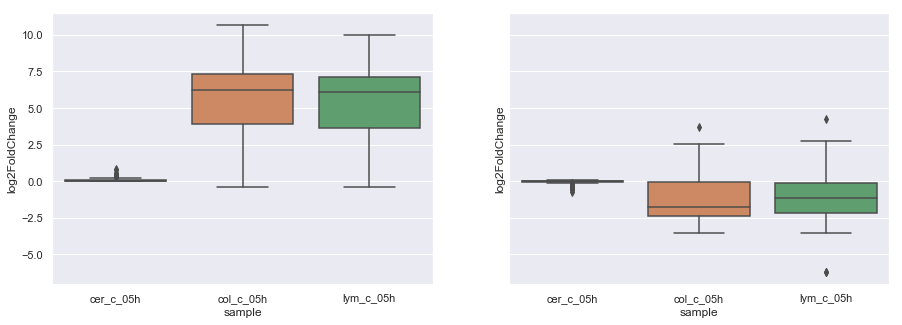
\includegraphics[width=.9\linewidth]{obipy-resources/pairings_05hr_boxplots.png}
\caption{\label{pairings_05hr_boxplots}
Boxplots of differential expressions from 50 largest (left) and 50 lowe05hst (right) DE genes}
\end{figure}


\clearpage\\

\section{6hr c/w}
\label{sec:orgd5e347e}

These treatments are comparing the X axis to their water treatments, not to each other, selection is done with the 10 most upregulated genes from each 3 genotypes, and pooled together for reference across genotypes.\\
 The second heatmap is the same, only it is downregulated top 10 for each\\

\begin{minted}[frame=lines,linenos=true,fontfamily=Monaco]{ipython}
DE_pairings_6hr = read_xl('/Users/hughesn/PHD/Transcripts/Data/pairings_6hr.xlsx')
\end{minted}

\subsection{Clustermap of largest/smallest DE genes}
\label{sec:org54e8b83}

\begin{minted}[frame=lines,linenos=true,fontfamily=Monaco]{ipython}
import matplotlib.pyplot as plt
import seaborn as sns
import numpy as np
%matplotlib inline
top, bot = get_two_clustermaps_data(DE_pairings_6hr, 25)
gt = sns.clustermap(top.set_index('gene name'), cmap='bwr', vmin=-10, vmax=10, yticklabels=True, figsize=(20,20))
\end{minted}

\begin{verbatim}
<Figure size 1440x1440 with 4 Axes>
\end{verbatim}


\begin{center}
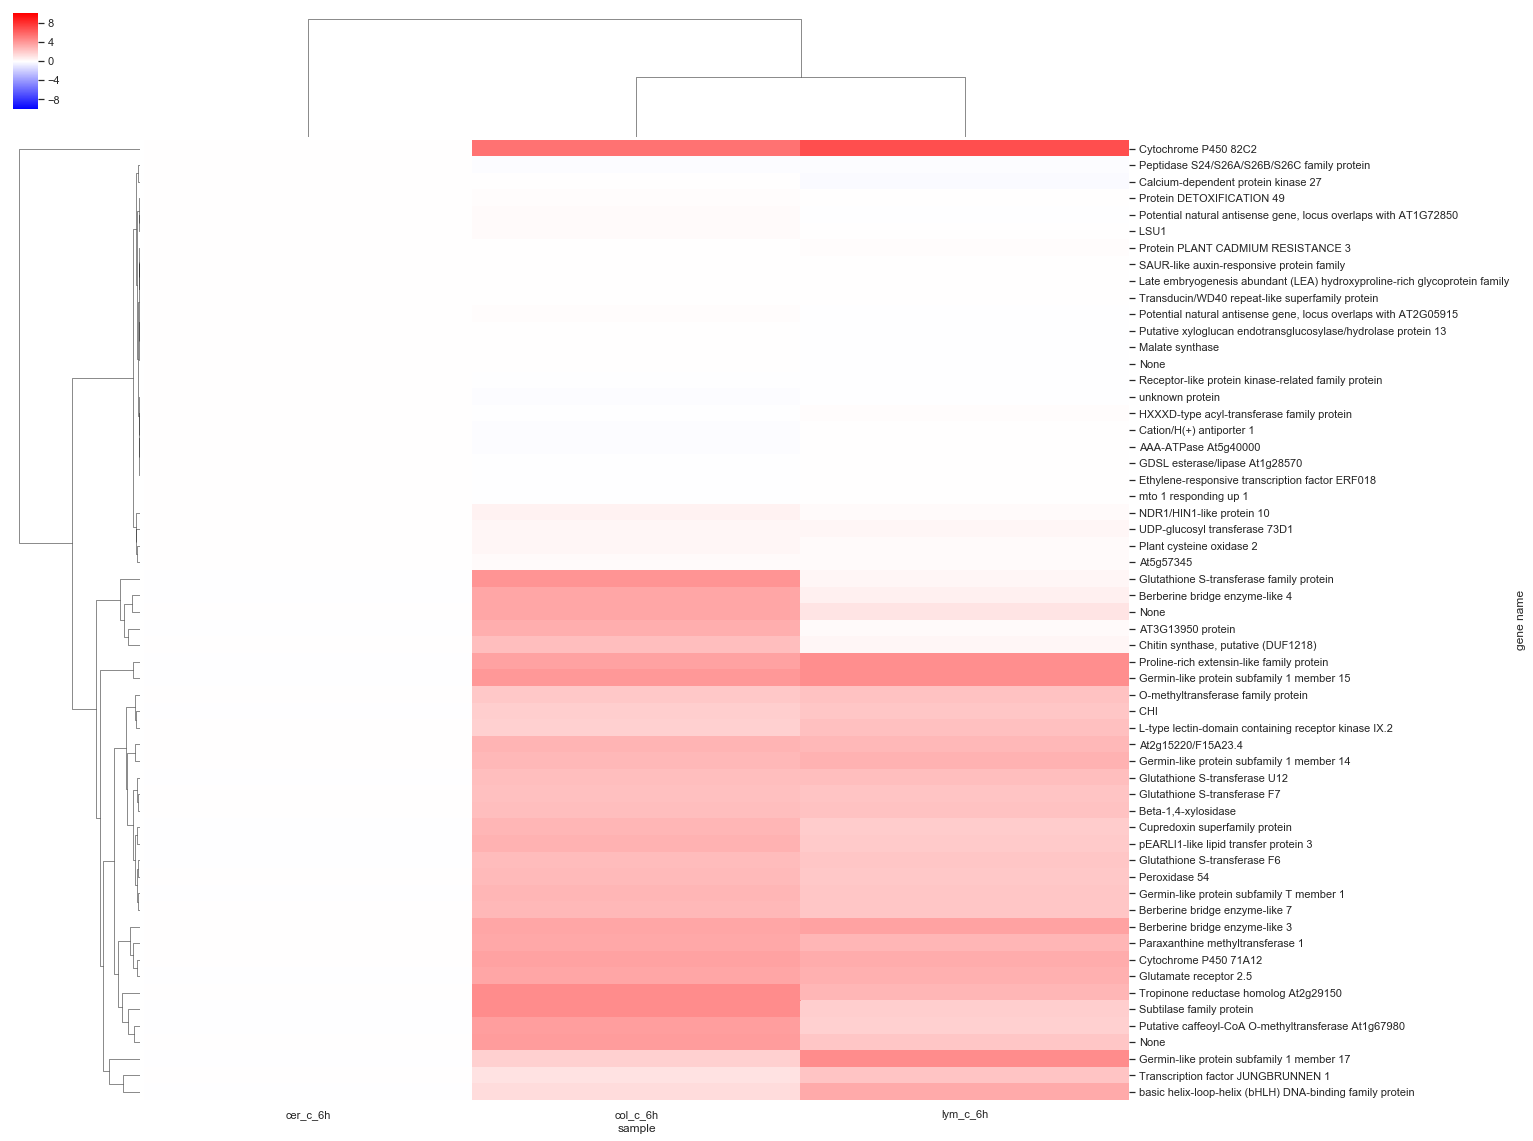
\includegraphics[width=.9\linewidth]{obipy-resources/e77a762dc857123716befe90c8377aaf6f2b9180/5a9a35854593758bab2621b6ad3a9b3594da2d1c.png}
\end{center}

\begin{center}
\begin{tabular}{lrrrl}
gene & cer\_c\_6h & col\_c\_6h & lym\_c\_6h & gene name\\
\hline
AT1G02920 & 4.956e-05 & 2.49449 & 2.26597 & Glutathione S-transferase F7\\
AT1G02930 & -7.22963e-05 & 2.58666 & 2.19736 & Glutathione S-transferase F6\\
AT1G08663 & 0.00421952 & 0.00437637 & -0.00674723 & None\\
AT1G16380 & 0.00467278 & -0.0816752 & 0.0653938 & Cation/H(+) antiporter 1\\
AT1G18970 & -0.000213452 & 2.86316 & 2.23722 & Germin-like protein subfamily T member 1\\
AT1G21120 & 0.0002184 & 2.13913 & 2.38183 & O-methyltransferase family protein\\
AT1G26240 & -7.43672e-05 & 3.60049 & 4.44481 & Proline-rich extensin-like family protein\\
AT1G26380 & 0.000314561 & 3.50937 & 3.62568 & Berberine bridge enzyme-like 3\\
AT1G26390 & -0.000244805 & 3.47501 & 0.598637 & Berberine bridge enzyme-like 4\\
AT1G26420 & 5.99864e-05 & 2.75806 & 2.25522 & Berberine bridge enzyme-like 7\\
AT1G28570 & 0.00913303 & -0.0430658 & 0.0645773 & GDSL esterase/lipase At1g28570\\
AT1G29460 & 0.00808904 & 0.021524 & 0.0512523 & SAUR-like auxin-responsive protein family\\
AT1G29960 & 0.0136508 & -0.107611 & -0.145689 & Peptidase S24/S26A/S26B/S26C family protein\\
AT1G31490 & 0.0105197 & -0.0367075 & 0.108269 & HXXXD-type acyl-transferase family protein\\
AT1G63600 & 0.00689469 & -0.00621645 & -0.0117278 & Receptor-like protein kinase-related family protein\\
AT1G66700 & 7.12184e-06 & 3.40873 & 2.81457 & Paraxanthine methyltransferase 1\\
AT1G67980 & -5.27256e-06 & 3.76495 & 1.87169 & Putative caffeoyl-CoA O-methyltransferase At1g67980\\
AT1G69920 & -9.98085e-05 & 2.50891 & 2.51402 & Glutathione S-transferase U12\\
AT1G72852 & 0.00826322 & 0.203518 & -0.00964083 & Potential natural antisense gene, locus overlaps with AT1G72850\\
AT1G74930 & 0.0101411 & -0.0294794 & 0.0427114 & Ethylene-responsive transcription factor ERF018\\
AT2G05914 & 0.0171099 & 0.0827773 & -0.0376694 & Potential natural antisense gene, locus overlaps with AT2G05915\\
AT2G15220 & 0.00269334 & 2.91898 & 2.79065 & At2g15220/F15A23.4\\
AT2G25297 & 0.00104608 & 3.84049 & 2.21879 & None\\
AT2G29150 & 9.59632e-05 & 4.46845 & 2.83809 & Tropinone reductase homolog At2g29150\\
AT2G30750 & 6.61106e-05 & 3.62051 & 3.21831 & Cytochrome P450 71A12\\
AT2G35980 & 0.00435733 & 0.504199 & 0.159604 & NDR1/HIN1-like protein 10\\
AT2G43000 & 0.000120952 & 1.10818 & 2.32787 & Transcription factor JUNGBRUNNEN 1\\
AT2G43570 & -0.000110251 & 1.94081 & 2.23337 & CHI\\
AT3G13950 & -3.0432e-05 & 3.19584 & 0.165878 & AT3G13950 protein\\
AT3G19615 & 0.000261642 & 2.5281 & 2.37951 & Beta-1,4-xylosidase\\
AT3G21305 & 9.59244e-05 & 3.45482 & 1.06607 & None\\
AT3G49580 & 0.00561342 & 0.160499 & 0.053971 & LSU1\\
AT3G53150 & 0.00700147 & 0.389497 & 0.360159 & UDP-glucosyl transferase 73D1\\
AT3G54200 & 0.00467572 & 0.0515371 & 0.0349536 & Late embryogenesis abundant (LEA) hydroxyproline-rich glycoprotein family\\
AT3G60270 & -0.000156181 & 2.85373 & 1.99023 & Cupredoxin superfamily protein\\
AT4G04700 & 0.0455861 & 0.0320945 & -0.168382 & Calcium-dependent protein kinase 27\\
AT4G10530 & -0.000108805 & 4.45945 & 1.92021 & Subtilase family protein\\
AT4G12500 & -0.000228082 & 3.00897 & 2.09654 & pEARLI1-like lipid transfer protein 3\\
AT4G19370 & 5.28087e-05 & 2.53867 & 0.31638 & Chitin synthase, putative (DUF1218)\\
AT4G23030 & 0.0440471 & 0.112794 & 0.00356702 & Protein DETOXIFICATION 49\\
AT4G31970 & 0.000222508 & 5.53636 & 6.93525 & Cytochrome P450 82C2\\
AT4G37095 & 0.00552418 & -0.0993937 & -0.00176731 & unknown protein\\
AT5G03860 & 0.00514605 & 0.0273616 & -0.0178313 & Malate synthase\\
AT5G06730 & 0.00055951 & 2.67853 & 2.14532 & Peroxidase 54\\
AT5G11210 & -0.000127495 & 3.50968 & 3.09579 & Glutamate receptor 2.5\\
AT5G35490 & 0.0153947 & -0.0228948 & 0.0519844 & mto 1 responding up 1\\
AT5G35525 & 0.00488355 & 0.0686101 & 0.0831995 & Protein PLANT CADMIUM RESISTANCE 3\\
AT5G39110 & 8.50824e-05 & 2.74372 & 3.00043 & Germin-like protein subfamily 1 member 14\\
AT5G39120 & -0.000104424 & 4.01959 & 4.38315 & Germin-like protein subfamily 1 member 15\\
AT5G39150 & -8.09123e-05 & 1.80213 & 4.48861 & Germin-like protein subfamily 1 member 17\\
AT5G39890 & 0.00590489 & 0.323962 & 0.195049 & Plant cysteine oxidase 2\\
AT5G40000 & 0.00628497 & -0.0791759 & 0.0528754 & AAA-ATPase At5g40000\\
AT5G44990 & -0.000105059 & 4.19897 & 0.312832 & Glutathione S-transferase family protein\\
AT5G54520 & 0.00710149 & 0.070907 & 0.016494 & Transducin/WD40 repeat-like superfamily protein\\
AT5G56960 & -5.06603e-06 & 1.38257 & 3.28386 & basic helix-loop-helix (bHLH) DNA-binding family protein\\
AT5G57345 & 0.00420978 & 0.177322 & 0.176793 & At5g57345\\
AT5G57540 & 0.00470175 & 0.0580137 & -0.048666 & Putative xyloglucan endotransglucosylase/hydrolase protein 13\\
AT5G65600 & 0.000205576 & 1.81817 & 2.42849 & L-type lectin-domain containing receptor kinase IX.2\\
\end{tabular}
\end{center}


\begin{minted}[frame=lines,linenos=true,fontfamily=Monaco]{ipython}
gb = sns.clustermap(bot.set_index('gene name'), cmap='bwr', vmin=-10, vmax=10, yticklabels=True, figsize=(20,20))
\end{minted}

\begin{verbatim}
<Figure size 1440x1440 with 4 Axes>
\end{verbatim}


\begin{center}
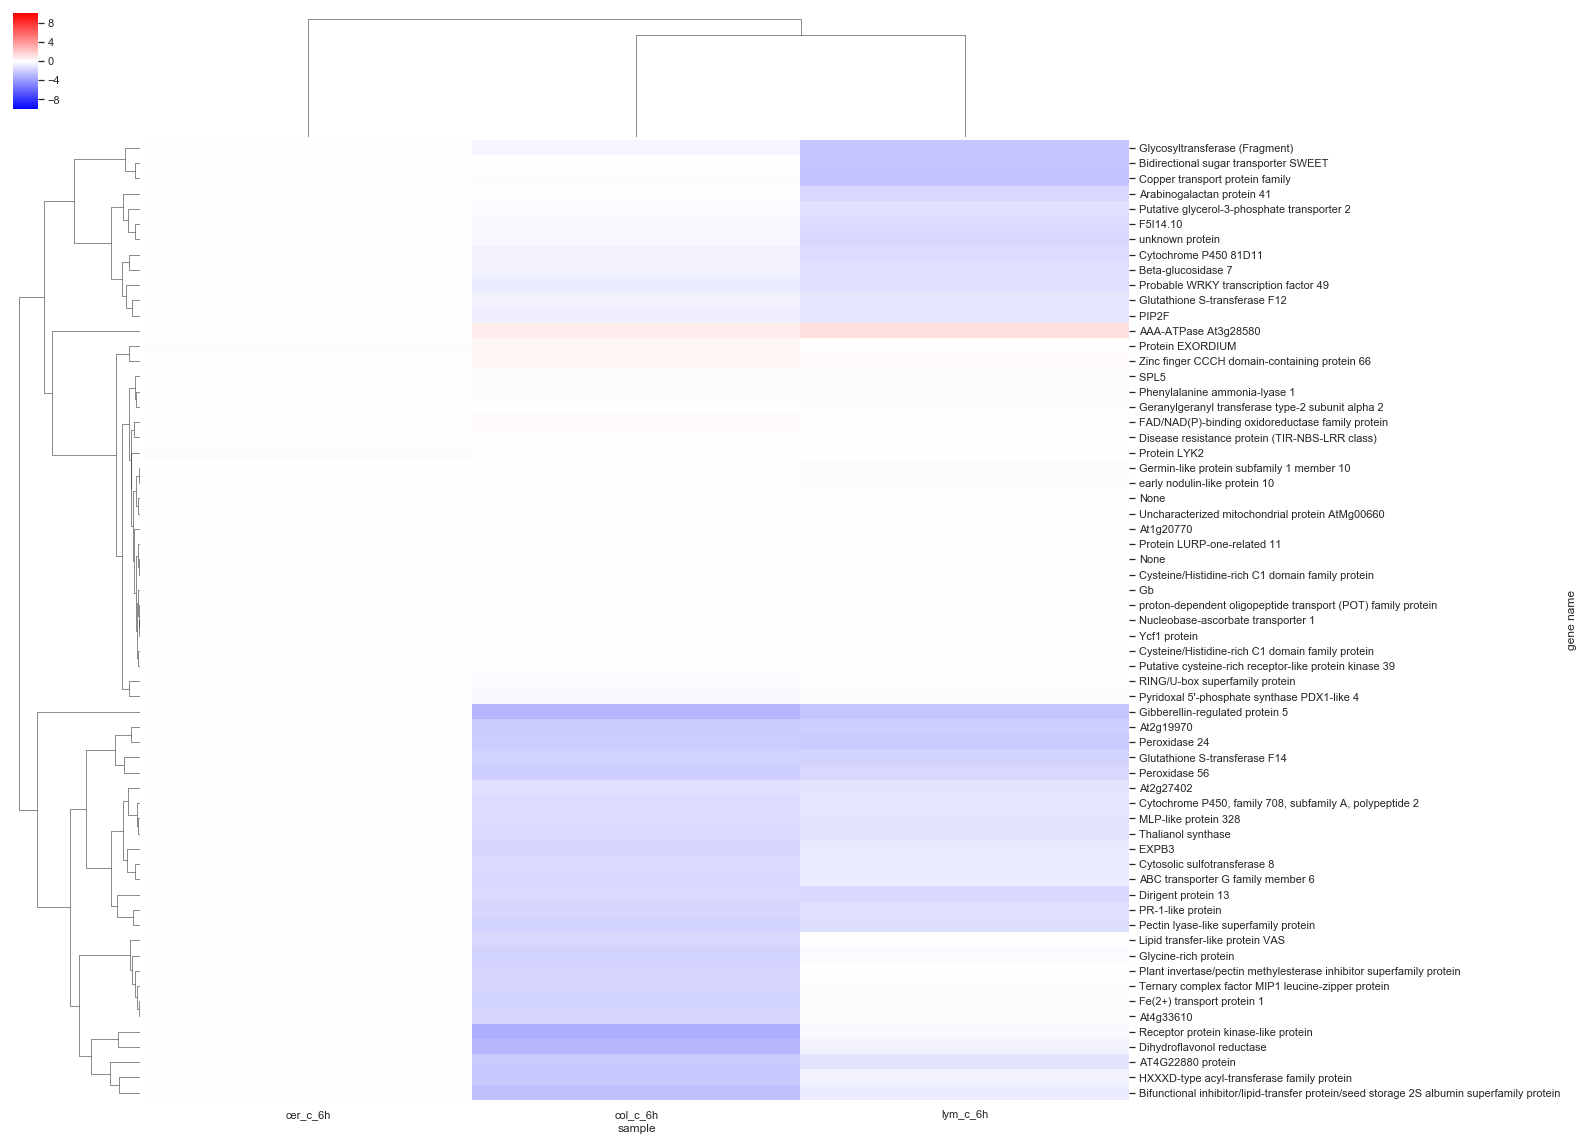
\includegraphics[width=.9\linewidth]{obipy-resources/e77a762dc857123716befe90c8377aaf6f2b9180/4c1c9e797663c4b195f56f4964a064754e2dfee3.png}
\end{center}


\begin{center}
\begin{tabular}{lrrrl}
gene & cer\_c\_6h & col\_c\_6h & lym\_c\_6h & gene name\\
\hline
AT1G13420 & 9.06555e-05 & -1.41823 & -0.820667 & Cytosolic sulfotransferase 8\\
AT1G20770 & -0.00759603 & 0.0350278 & 0.121528 & At1g20770\\
AT1G49860 & 9.88306e-05 & -1.79032 & -1.78761 & Glutathione S-transferase F14\\
AT1G55990 & -3.22815e-05 & -1.79485 & -0.215851 & Glycine-rich protein\\
AT1G65570 & -0.000171597 & -0.25407 & -1.3913 & F5I14.10\\
AT1G67856 & -0.0050584 & -0.228611 & 0.0658332 & RING/U-box superfamily protein\\
AT1G78990 & -9.26476e-05 & -2.18412 & -0.536063 & HXXXD-type acyl-transferase family protein\\
AT2G01520 & 0.000536664 & -1.38769 & -1.03726 & MLP-like protein 328\\
AT2G05760 & -0.00720883 & 0.0238018 & -0.00512061 & Nucleobase-ascorbate transporter 1\\
AT2G07638 & -0.0215611 & 0.0132227 & 0.0572107 & None\\
AT2G07739 & -0.00726359 & 0.0304755 & -0.0138274 & Ycf1 protein\\
AT2G09340 & -0.0115119 & 0.0555915 & -0.0694685 & None\\
AT2G19970 & -0.000211881 & -2.07101 & -1.94121 & At2g19970\\
AT2G19990 & -1.53578e-05 & -1.62935 & -1.22451 & PR-1-like protein\\
AT2G27402 & -0.000718984 & -1.2092 & -1.03675 & At2g27402\\
AT2G29720 & -0.00804433 & 0.213603 & -0.0509745 & FAD/NAD(P)-binding oxidoreductase family protein\\
AT2G37040 & -0.00490377 & -0.0959371 & -0.133422 & Phenylalanine ammonia-lyase 1\\
AT2G38100 & -0.00508613 & 0.00560105 & -0.0125254 & proton-dependent oligopeptide transport (POT) family protein\\
AT2G38210 & -0.0189151 & -0.310782 & -0.11573 & Pyridoxal 5'-phosphate synthase PDX1-like 4\\
AT2G39040 & -4.52948e-05 & -2.02658 & -2.09906 & Peroxidase 24\\
AT3G01840 & -0.143582 & 0.0600383 & -0.0243056 & Protein LYK2\\
AT3G02885 & -0.000311314 & -2.82663 & -2.22129 & Gibberellin-regulated protein 5\\
AT3G14260 & -0.00586598 & -0.0105797 & 0.0701973 & Protein LURP-one-related 11\\
AT3G15270 & -0.0717464 & -0.122205 & -0.0935992 & SPL5\\
AT3G18900 & -0.000166756 & -1.69521 & -0.103876 & Ternary complex factor MIP1 leucine-zipper protein\\
AT3G28580 & -0.0129667 & 0.766622 & 1.3174 & AAA-ATPase At3g28580\\
AT3G28740 & -0.00040857 & -0.519014 & -1.37452 & Cytochrome P450 81D11\\
AT3G46270 & -0.000204056 & -3.14195 & -0.292378 & Receptor protein kinase-like protein\\
AT3G48400 & -0.00552687 & 0.0592092 & 0.0120445 & Cysteine/Histidine-rich C1 domain family protein\\
AT3G49330 & 0.000150711 & -1.66602 & -0.0568086 & Plant invertase/pectin methylesterase inhibitor superfamily protein\\
AT3G62740 & 0.00240045 & -0.482753 & -1.18895 & Beta-glucosidase 7\\
AT4G04540 & -0.0426056 & 0.0540724 & 0.0289514 & Putative cysteine-rich receptor-like protein kinase 39\\
AT4G08950 & -0.139356 & 0.389032 & 0.0340314 & Protein EXORDIUM\\
AT4G11190 & 7.30769e-05 & -1.42737 & -1.53854 & Dirigent protein 13\\
AT4G15290 & -9.23775e-05 & -0.33117 & -2.33806 & Glycosyltransferase (Fragment)\\
AT4G16015 & -0.00468678 & 0.0281886 & 0.0524822 & Cysteine/Histidine-rich C1 domain family protein\\
AT4G19690 & -0.000192642 & -1.73413 & -0.152767 & Fe(2+) transport protein 1\\
AT4G22880 & -6.72331e-05 & -2.04061 & -1.02763 & AT4G22880 protein\\
AT4G24265 & 1.35819e-05 & -0.235625 & -1.48487 & unknown protein\\
AT4G25220 & -0.000186362 & -0.22562 & -1.2254 & Putative glycerol-3-phosphate transporter 2\\
AT4G28250 & 3.70609e-06 & -1.68035 & -0.801688 & EXPB3\\
AT4G33610 & 7.66466e-05 & -1.7142 & -0.146025 & At4g33610\\
AT5G05300 & -0.00869039 & 0.00337846 & 0.0205706 & Gb\\
AT5G13580 & 4.85555e-05 & -1.49453 & -0.775036 & ABC transporter G family member 6\\
AT5G13900 & 9.65328e-05 & -1.55886 & -0.0700806 & Lipid transfer-like protein VAS\\
AT5G14650 & -0.000398461 & -1.74474 & -1.25928 & Pectin lyase-like superfamily protein\\
AT5G15180 & 0.00015035 & -1.89009 & -1.53507 & Peroxidase 56\\
AT5G17220 & -0.000105446 & -0.524166 & -0.986159 & Glutathione S-transferase F12\\
AT5G24105 & -2.51795e-05 & 0.00365151 & -1.49988 & Arabinogalactan protein 41\\
AT5G38930 & -0.00470097 & 0.0183421 & -0.114339 & Germin-like protein subfamily 1 member 10\\
AT5G41820 & -0.00610108 & -0.0398202 & -0.0896063 & Geranylgeranyl transferase type-2 subunit alpha 2\\
AT5G42800 & -0.000108875 & -2.82511 & -0.518265 & Dihydroflavonol reductase\\
AT5G43290 & 1.28897e-05 & -0.72002 & -1.17867 & Probable WRKY transcription factor 49\\
AT5G45240 & -0.0314374 & 0.128619 & -0.00867202 & Disease resistance protein (TIR-NBS-LRR class)\\
AT5G46890 & 4.23551e-05 & -2.49004 & -0.746737 & Bifunctional inhibitor/lipid-transfer protein/seed storage 2S albumin superfamily protein\\
AT5G48000 & 6.5311e-05 & -1.4041 & -0.972066 & Cytochrome P450, family 708, subfamily A, polypeptide 2\\
AT5G48010 & 9.33774e-05 & -1.42574 & -1.01972 & Thalianol synthase\\
AT5G50800 & 1.5557e-06 & -0.0249659 & -2.33902 & Bidirectional sugar transporter SWEET\\
AT5G52710 & 0.000246235 & -0.107855 & -2.35584 & Copper transport protein family\\
AT5G57920 & -0.00618138 & 0.0287925 & -0.124408 & early nodulin-like protein 10\\
AT5G58620 & -0.00630026 & 0.336247 & 0.171014 & Zinc finger CCCH domain-containing protein 66\\
AT5G60660 & -0.000167615 & -0.654489 & -0.961522 & PIP2F\\
ATMG00660 & -0.00543698 & 0.0184692 & -0.0468381 & Uncharacterized mitochondrial protein AtMg00660\\
\end{tabular}
\end{center}




\subsection{Boxplots of differential changes}
\label{sec:org981bdaa}

\begin{verbatim}
<Figure size 1080x360 with 2 Axes>
\end{verbatim}


\begin{figure}[htbp]
\centering
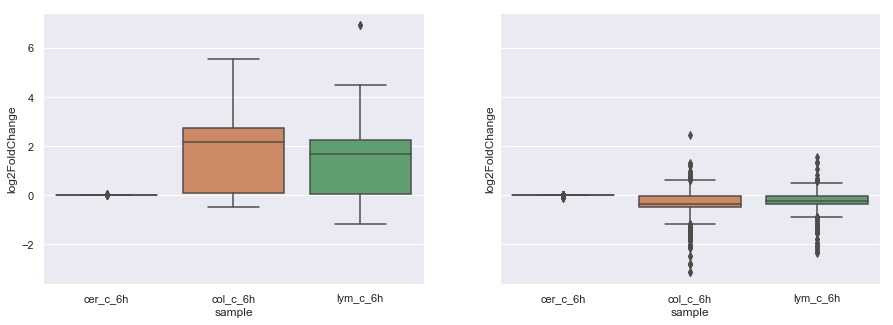
\includegraphics[width=.9\linewidth]{obipy-resources/pairings_6hr_boxplots.png}
\caption{\label{pairings_6hr_boxplots}
Boxplots of differential expressions from 50 largest (left) and 50 lowest (right) DE genes}
\end{figure}



\clearpage\\
\section{lym 05hr c/w}
\label{sec:orgd14ed54}

These treatments are comparing the X axis to their lym counter part. e.g. cer\_w is compared to lym\_w and col\_c is compared to lym\_c.\\

\begin{minted}[frame=lines,linenos=true,fontfamily=Monaco]{ipython}
DE_pairings_to_lym_05hr = read_xl('/Users/hughesn/PHD/Transcripts/Data/pairings_to_lym_05hr.xlsx')
\end{minted}

\subsection{Clustermap of largest/smallest DE genes}
\label{sec:orga1800e1}

\begin{minted}[frame=lines,linenos=true,fontfamily=Monaco]{ipython}
import matplotlib.pyplot as plt
import seaborn as sns
import numpy as np
%matplotlib inline
top, bot = get_two_clustermaps_data(DE_pairings_to_lym_05hr, 25)
gt = sns.clustermap(top.set_index('gene name'), cmap='bwr', vmin=-10, vmax=10, yticklabels=True, figsize=(20,20))
\end{minted}

\begin{verbatim}
<Figure size 1440x1440 with 4 Axes>
\end{verbatim}


\begin{center}
\includegraphics[width=.9\linewidth]{obipy-resources/e77a762dc857123716befe90c8377aaf6f2b9180/6f17bf3e5001a7f47ad172f570ac9ab1562e4a5c.png}
\end{center}

\begin{center}
\begin{tabular}{lrrrrl}
gene & cer\_c\_05h & cer\_w\_05h & col\_c\_05h & col\_w\_05h & gene name\\
\hline
AT1G01580 & 0.927797 & 3.01653 & -0.00378893 & 0.00564039 & ferric reduction oxidase 2\\
AT1G01660 & -0.282569 & 0.277395 & 0.00138677 & 0.59823 & RING/U-box superfamily protein\\
AT1G04797 & 2.83853 & 0.0549455 & 0 & 0.00186046 & None\\
AT1G05867 & 2.96684 & 1.67177 & 2.60465 & 1.28893 & None\\
AT1G07887 & 2.11295 & 0.182659 & 0.347947 & 0.142045 & None\\
AT1G12040 & -0.825821 & 0.0452786 & 0.00305099 & 0.535019 & Leucine-rich repeat extensin-like protein 1\\
AT1G12560 & -0.541185 & 0.0168151 & 0.00203194 & 0.745438 & Expansin\\
AT1G16510 & 3.10775 & 1.43097 & -0.000112732 & -0.00133502 & Auxin-responsive protein SAUR41\\
AT1G21250 & 1.85817 & 1.98169 & -0.000424165 & -0.0289893 & Wall-associated receptor kinase 1\\
AT1G24280 & 2.91547 & 1.62332 & 2.09986 & 1.11792 & Glucose-6-phosphate 1-dehydrogenase\\
AT1G26250 & -0.585518 & 0.265608 & 0.0181645 & 0.569356 & Proline-rich extensin-like family protein\\
AT1G26255 & -0.676483 & 0.270886 & 0.00633239 & 0.489692 & None\\
AT1G29020 & 0.75084 & 2.25945 & 0.00403511 & 0.0825415 & Calcium-binding EF-hand family protein\\
AT1G31173 & 5.74866 & -0.0272493 & 0.0602687 & -0.000165912 & MIR167D\\
AT1G33960 & 1.3799 & 2.0337 & 0.00163937 & -0.00186199 & P-loop containing nucleoside triphosphate hydrolases superfamily protein\\
AT1G45145 & -0.401337 & 0.308364 & 0.00100613 & 0.844821 & Thioredoxin H5\\
AT1G53480 & 3.87345 & 3.23021 & 4.56819 & 3.73034 & Mto 1 responding down 1\\
AT1G53490 & 0.257724 & 0.173043 & 0.355824 & 0.0193441 & E3 ubiquitin-protein ligase CCNB1IP1 homolog\\
AT1G53541 & 1.02145 & 0.0232522 & 0.251917 & 0.00700338 & unknown protein\\
AT1G56650 & 3.50514 & 1.71161 & 0.0028148 & -0.00175443 & Transcription factor MYB75\\
AT1G61800 & 3.30498 & 2.48906 & 0.00298561 & 0.00757727 & glucose-6-phosphate/phosphate translocator 2\\
AT1G69880 & 1.01512 & 0.519532 & 0.267205 & 0.0952865 & Thioredoxin H8\\
AT1G75945 & 4.7667 & 4.57281 & -0.00446997 & -0.00701536 & None\\
AT1G79110 & 2.84655 & 0.359723 & -0.00415798 & -0.0556011 & Probable BOI-related E3 ubiquitin-protein ligase 2\\
AT2G14560 & 0.614338 & 2.11427 & -0.00201486 & -0.00665759 & Protein of unknown function (DUF567)\\
AT2G15220 & -3.65887 & 0.0179649 & 0.000589872 & 0.858102 & At2g15220/F15A23.4\\
AT2G17120 & -0.356764 & 2.56485 & 0.861042 & 2.3745 & LysM domain-containing GPI-anchored protein 2\\
AT2G23150 & 0.0909341 & 0.0350633 & 0.295938 & -0.0146497 & Metal transporter Nramp3\\
AT2G24850 & 1.92114 & 2.92074 & 0.00356544 & 0.00415556 & Probable aminotransferase TAT3\\
AT2G25470 & -0.353965 & 2.01204 & -0.00438498 & 0.012819 & receptor like protein 21\\
AT2G30770 & 2.77252 & 1.56742 & 0.00282876 & 0.0116375 & Indoleacetaldoxime dehydratase\\
AT2G33620 & 0.417682 & 0.13063 & 0.258241 & -0.0177558 & AT-hook motif nuclear-localized protein 10\\
AT2G36750 & 3.08164 & 0.259822 & 0.171328 & 0.0315722 & UDP-glycosyltransferase 73C1\\
AT2G42350 & -1.63482 & 0.628376 & -0.000790481 & 0.876192 & RING-H2 finger protein ATL40\\
AT2G43120 & -0.381775 & 0.285545 & 0.00421295 & 0.667526 & RmlC-like cupins superfamily protein\\
AT2G45570 & 1.73123 & -0.0375818 & 0.659625 & 0.00582304 & Cytochrome P450 76C2\\
AT2G47440 & 0.469128 & 0.0195286 & 0.0379141 & 0.617122 & Tetratricopeptide repeat (TPR)-like superfamily protein\\
AT3G08690 & 0.794027 & 1.19422 & 0.590676 & 0.666151 & Ubiquitin-conjugating enzyme E2 11\\
AT3G10525 & 1.42479 & 0.0844429 & 0.229849 & 0.000745217 & SMR1\\
AT3G10710 & -0.208872 & 0.219531 & 0.00152052 & 0.548569 & Putative pectinesterase/pectinesterase inhibitor 24\\
AT3G12955 & 0.125063 & -0.0268408 & 0.469286 & 0.00536118 & At3g12955\\
AT3G16360 & 2.2911 & 2.32221 & 0.00666119 & 0.112823 & AHP4\\
AT3G17580 & 2.85769 & 0.0205339 & 0.00401815 & 0.00449532 & SsrA-binding protein\\
AT3G18860 & 1.77959 & 1.73585 & 1.79144 & 1.60692 & AT3g18860/MCB22\_3\\
AT3G21500 & 1.40203 & 0.0206241 & 0.256699 & -0.00647619 & 1-deoxy-D-xylulose 5-phosphate synthase 1\\
AT3G21620 & 5.41903 & 5.00278 & 0.00020351 & 0.0148633 & CSC1-like protein At3g21620\\
AT3G23120 & -0.023148 & 1.93108 & -0.00757574 & -0.0152237 & Receptor-like protein 38\\
AT3G28740 & -0.451132 & 0.00471883 & 0.00553966 & 2.38573 & Cytochrome P450 81D11\\
AT3G45940 & 2.93504 & -0.00411077 & 0.0165615 & 0.00356093 & Putative alpha-xylosidase 2\\
AT3G48120 & 0.755183 & 0.107992 & 0.943718 & 0.00416738 & At3g48120\\
AT3G50770 & 0.523652 & 2.21119 & -0.0011893 & -0.00239834 & Probable calcium-binding protein CML41\\
AT4G08950 & -1.52928 & 0.0288968 & 0.0975284 & 0.619601 & Protein EXORDIUM\\
AT4G09820 & 3.27365 & 2.23681 & 0.0549639 & 0.0220741 & Transcription factor TT8\\
AT4G09890 & 1.2066 & -0.0811051 & 0.282123 & 0.00886576 & At4g09890\\
AT4G12320 & 0.257967 & -0.0102678 & 0.346427 & 0.161401 & At4g12320\\
AT4G12490 & 1.97753 & 2.38026 & 0.00636406 & 0.047948 & pEARLI1-like lipid transfer protein 2\\
AT4G12495 & 2.0838 & 2.38864 & 0.0170266 & 0.0439778 & Transmembrane protein\\
AT4G12500 & 1.59671 & 3.04143 & 0.000524352 & 0.235614 & pEARLI1-like lipid transfer protein 3\\
AT4G19690 & 3.67259 & 1.96402 & 0.00212744 & 0.0100143 & Fe(2+) transport protein 1\\
AT4G22880 & 4.50756 & 1.12498 & 0.00588695 & 0.00560844 & AT4G22880 protein\\
AT4G25220 & -0.64532 & 1.291 & 0.00470425 & 1.37067 & Putative glycerol-3-phosphate transporter 2\\
AT4G26840 & 0.468 & 0.0489624 & 0.303887 & 0.00264802 & Small ubiquitin-related modifier 1\\
AT4G26950 & 3.85384 & 0.422406 & 0.0126382 & -0.0763949 & At4g26950\\
AT4G28850 & -0.703141 & 0.122009 & 0.000424231 & 0.792137 & Probable xyloglucan endotransglucosylase/hydrolase protein 26\\
AT4G31354 & 2.87312 & 0.173494 & 0.0108425 & 0.00338942 & unknown protein\\
AT4G37990 & 1.8598 & 0.106097 & 0.422882 & 0.00255351 & Cinnamyl alcohol dehydrogenase 8\\
AT4G38850 & 4.01463 & 0.0247084 & 0.0970196 & 0.018867 & Auxin-responsive protein SAUR15\\
AT4G39210 & 2.40286 & 1.86605 & 0.00547067 & 0.00699041 & Glucose-1-phosphate adenylyltransferase\\
AT5G03350 & 2.30708 & 1.99791 & 0.00277281 & 0.00643833 & Lectin-like protein\\
AT5G07360 & 0.18942 & 0.0132137 & 0.491245 & 0.0269219 & Amidase family protein\\
AT5G10300 & 0.0668829 & 0.0860039 & -0.00162626 & 0.576921 & Alpha-hydroxynitrile lyase\\
AT5G17220 & 2.81654 & 1.39872 & 0.00327213 & 0.00511684 & Glutathione S-transferase F12\\
AT5G24200 & 0.885085 & 2.19007 & 0.00348039 & -0.00410725 & alpha/beta-Hydrolases superfamily protein\\
AT5G25340 & 1.65266 & 0.222407 & 0.000145694 & 0.641121 & Ubiquitin-like superfamily protein\\
AT5G42800 & 4.37776 & 0.595222 & 0.00631842 & 0.00417944 & Dihydroflavonol reductase\\
AT5G44575 & 1.22455 & 1.89149 & -0.00222962 & 0.0030017 & At5g44575\\
AT5G47330 & 2.05929 & 0.549176 & 0.847592 & 0.00627269 & Alpha/beta-Hydrolases superfamily protein\\
AT5G51850 & 3.30889 & 0.0357217 & 0.0564735 & -0.0228934 & TRM24\\
AT5G54060 & 3.39854 & 0.296381 & 0.00151917 & 0.00420788 & Glycosyltransferase (Fragment)\\
AT5G54640 & 1.24075 & 0.0626886 & 0.332738 & 0.00824407 & Histone H2A.6\\
AT5G55050 & 0.476577 & 1.80037 & -0.00206453 & 0.00727583 & GDSL esterase/lipase At5g55050\\
AT5G57530 & -0.0808817 & 0.273855 & 0.0122321 & 0.760887 & Probable xyloglucan endotransglucosylase/hydrolase protein 12\\
AT5G65613 & 1.28194 & 0.185879 & 0.237245 & 0.0462274 & None\\
AT5G67400 & -0.530316 & 0.154667 & 0.00114878 & 0.544571 & Peroxidase\\
\end{tabular}
\end{center}


\begin{minted}[frame=lines,linenos=true,fontfamily=Monaco]{ipython}
gb = sns.clustermap(bot.set_index('gene name'), cmap='bwr', vmin=-10, vmax=10, yticklabels=True, figsize=(20,20))
\end{minted}

\begin{verbatim}
<Figure size 1440x1440 with 4 Axes>
\end{verbatim}


\begin{center}
\includegraphics[width=.9\linewidth]{obipy-resources/e77a762dc857123716befe90c8377aaf6f2b9180/ea6a8531ef01419b250ad1f6258fe88224f17281.png}
\end{center}


\begin{center}
\begin{tabular}{lrrrrl}
gene & cer\_c\_05h & cer\_w\_05h & col\_c\_05h & col\_w\_05h & gene name\\
\hline
AT1G05767 & -6.87697 & 0.0193297 & -0.00200955 & 0 & None\\
AT1G07160 & -7.15426 & -0.056058 & 0.00124552 & -0.0124115 & PP2C-type phosphatase AP2C2\\
AT1G08650 & 0.535548 & 0.00785174 & -0.784357 & -0.0512296 & Phosphoenolpyruvate carboxylase kinase 1\\
AT1G10130 & -0.468707 & -0.181297 & -0.439827 & -0.377277 & Calcium-transporting ATPase 3, endoplasmic reticulum-type\\
AT1G10300 & 0.417538 & 0.00348659 & 0.0108669 & -0.293996 & Nucleolar GTP-binding protein 1\\
AT1G14540 & -6.58942 & -0.142143 & -0.00145164 & -0.0165351 & Peroxidase\\
AT1G14550 & -7.92058 & -0.0719554 & -0.000808195 & 0.00652742 & Peroxidase 5\\
AT1G21326 & -6.81027 & -0.0285366 & 0.000972512 & -0.0018448 & F16F4.1 protein\\
AT1G54650 & 0.307322 & -0.110777 & 0.00167732 & -0.551061 & Methyltransferase family protein\\
AT1G56240 & -6.66863 & -0.0410878 & -0.00099873 & -0.00636639 & F-box protein PP2-B13\\
AT1G56242 & -6.69012 & -0.236072 & -0.00136997 & -0.0157472 & other RNA\\
AT1G56250 & -6.87883 & -0.0809658 & -0.0015092 & -0.000150076 & F-box protein VBF\\
AT1G62720 & -2.01359 & -0.0140251 & -2.40631 & -0.0125105 & Pentatricopeptide repeat-containing protein At1g62720\\
AT1G62730 & -3.25733 & -0.0639644 & -3.61446 & -0.409654 & At1g62730\\
AT1G62740 & -2.71381 & -0.771658 & -2.76356 & -0.872567 & Hsp70-Hsp90 organizing protein 2\\
AT1G65370 & 0.143271 & -0.476627 & -0.0063646 & -0.280946 & At1g65370/T8F5\_15\\
AT1G66800 & -2.10786 & -1.90101 & 0.0021134 & 0.0273842 & NAD(P)-binding Rossmann-fold superfamily protein\\
AT1G67105 & -1.47402 & -1.83457 & -0.00194414 & -0.00960399 & other RNA\\
AT1G68190 & -1.41452 & -1.45952 & -0.000949812 & 0.0387351 & B-box zinc finger family protein\\
AT1G70610 & -0.353357 & -0.153479 & -0.320035 & 0.000972646 & ABC transporter B family member 26, chloroplastic\\
AT1G79680 & -6.42744 & -0.107625 & -0.000939944 & -0.0117586 & Wall-associated receptor kinase-like 10\\
AT2G01520 & -2.63874 & -1.8686 & -0.00258625 & 0.0133392 & MLP-like protein 328\\
AT2G05675 & -0.713511 & -0.527623 & -0.0216537 & -0.401098 & None\\
AT2G05914 & -2.52477 & -2.8757 & -1.69272 & -1.97508 & Potential natural antisense gene, locus overlaps with AT2G05915\\
AT2G05915 & -3.32258 & -2.85269 & -1.87077 & -1.552 & unknown protein\\
AT2G20570 & 0.959169 & 0.208169 & -0.0109891 & -0.335452 & GBF's pro-rich region-interacting factor 1\\
AT2G23270 & -8.10813 & 0.0158928 & 0.000182586 & 0.00773432 & At2g23270\\
AT2G25900 & -1.49345 & -1.52345 & -0.0056388 & 0.0119997 & Zinc finger CCCH domain-containing protein 23\\
AT2G28110 & -0.123137 & -1.6184 & 0.00244676 & 0.0092965 & Glycosyltransferase (Fragment)\\
AT2G29100 & -7.5596 & 0.0392355 & -0.00190841 & 0.00591816 & Glutamate receptor\\
AT2G29110 & -7.55585 & -0.0129176 & 0.00128308 & -0.0113225 & Glutamate receptor\\
AT2G31345 & -7.21108 & 0.00315754 & 0.00691887 & 0.000266106 & Transmembrane protein\\
AT2G32240 & -0.580707 & 0.055217 & -0.246447 & 0.0126289 & FUNCTIONS IN: molecular\_function unknown\\
AT2G33480 & 0.45563 & -0.0287836 & -0.510825 & -0.00669038 & NAC domain-containing protein 41\\
AT2G36440 & -7.07566 & 0.0181883 & 0.000921324 & 0.00272979 & Uncharacterized protein At2g36440\\
AT2G36690 & -3.3458 & -0.31344 & -0.00307618 & -0.392983 & 2-oxoglutarate (2OG) and Fe(II)-dependent oxygenase superfamily protein\\
AT2G36910 & -1.61867 & 0.0268254 & -1.60947 & -0.0922756 & ABC transporter B family member 1\\
AT2G38290 & -0.606489 & 0.259443 & -0.237973 & -0.0274771 & Ammonium transporter 2\\
AT2G39510 & -0.740404 & -1.35534 & -0.000463035 & -0.0242065 & WAT1-related protein At2g39510\\
AT2G47920 & -2.76838 & -0.252699 & -2.97669 & -0.0216259 & Protein NETWORKED 3C\\
AT3G01165 & -6.45047 & 0.0752788 & 0.0058913 & -0.0087008 & None\\
AT3G02840 & -6.45162 & 0.0399438 & 0.000926084 & -0.000656433 & ARM repeat superfamily protein\\
AT3G06355 & -0.747675 & -1.25835 & -0.0156987 & -0.760046 & None\\
AT3G08700 & -4.85618 & -0.203244 & -4.94345 & -0.146505 & Probable ubiquitin-conjugating enzyme E2 12\\
AT3G13065 & -0.397179 & -1.42013 & 0.000706399 & -0.0014391 & Protein STRUBBELIG-RECEPTOR FAMILY 4\\
AT3G15450 & -2.15329 & -1.61088 & 0.00395889 & 0.118012 & AT3g15450/MJK13\_11\\
AT3G19430 & 0.67824 & 0.101886 & -0.00138637 & -0.288754 & Late embryogenesis abundant protein-related / LEA protein-like protein\\
AT3G23880 & -0.233054 & -1.70768 & 0.00268363 & -0.0147595 & F-box/kelch-repeat protein At3g23880\\
AT3G29644 & 0.237442 & 0.104231 & -0.83467 & -0.0322438 & other RNA\\
AT3G30720 & -0.700171 & -1.41971 & -2.54312 & -2.26491 & Protein QQS\\
AT3G47420 & 1.12852 & 0.0750028 & -0.0228686 & -0.791602 & Putative glycerol-3-phosphate transporter 1\\
AT3G48360 & -2.23365 & -1.53408 & 0.0430616 & 0.126198 & BTB/POZ and TAZ domain-containing protein 2\\
AT3G48630 & -6.79922 & 0.0370597 & -0.00197491 & 0 & unknown protein\\
AT4G02880 & -0.444716 & -0.624969 & -0.653412 & -0.394978 & unknown protein\\
AT4G02890 & -0.623899 & -0.804643 & -0.991224 & -0.841776 & Polyubiquitin 14\\
AT4G03610 & -0.21538 & -1.35471 & 0.00019488 & 0.00230334 & Metallo-hydrolase/oxidoreductase superfamily protein\\
AT4G04223 & -1.87467 & -1.43225 & 0.000795666 & -0.0468574 & other RNA\\
AT4G04335 & -0.612589 & -0.887493 & -0.928062 & -0.927047 & None\\
AT4G04480 & -8.01312 & 0 & -0.00148436 & 0 & F-box protein with a domain protein\\
AT4G05050 & -0.855292 & -0.61805 & -0.387599 & -0.613613 & Polyubiquitin\\
AT4G05320 & -0.642136 & -0.822933 & -0.859336 & -0.674265 & Polyubiquitin 10\\
AT4G08815 & -1.55709 & -1.89316 & 0.000757096 & -0.00120153 & None\\
AT4G11470 & -7.53383 & -0.00267271 & -0.000453368 & -0.000772484 & cysteine-rich RLK (RECEPTOR-like protein kinase) 31\\
AT4G22030 & -9.15372 & 0.0194823 & 0.0017636 & 0 & F-box family protein with a domain of unknown function (DUF295)\\
AT4G24180 & 0.0368866 & -1.36778 & 0.00376795 & -0.00646403 & THAUMATIN-LIKE PROTEIN 1\\
AT4G28460 & -8.90795 & 0.0245379 & 0.000218674 & -0.00835151 & PAMP-induced secreted peptide 1\\
AT4G31950 & -7.76344 & -0.0144101 & -0.0013043 & 0.000220636 & CYP82C3\\
AT4G33060 & -0.291125 & 0.152415 & -0.258438 & 0.00978603 & Peptidyl-prolyl cis-trans isomerase CYP57\\
AT4G33666 & -2.46428 & -1.51029 & -0.00233898 & 0.019046 & Uncharacterized protein At4g33666\\
AT5G03240 & -0.740667 & -1.04918 & -0.855993 & -0.488128 & Ubiquitin 4\\
AT5G07130 & -2.60889 & -2.96222 & -0.00363301 & -0.00549834 & Laccase-13\\
AT5G11140 & -8.98961 & -0.0450597 & 0.0169368 & -0.00750234 & Phospholipase-like protein (PEARLI 4) family protein\\
AT5G20150 & -0.254021 & -0.155154 & -0.549847 & -0.749813 & SPX domain-containing protein 1\\
AT5G20620 & -0.483054 & -0.858438 & -1.18019 & -1.01999 & Polyubiquitin 4\\
AT5G23840 & -2.03556 & -1.62524 & -0.000532914 & 0.0238845 & MD-2-related lipid recognition domain-containing protein\\
AT5G24110 & -8.44419 & 0.0258449 & -0.00137166 & -0.0050904 & Probable WRKY transcription factor 30\\
AT5G26290 & -0.155939 & -1.45044 & 0.00689551 & 0.0254486 & TRAF-like family protein\\
AT5G47710 & -0.887754 & -0.104207 & 0.000719494 & -0.620296 & Protein C2-DOMAIN ABA-RELATED 11\\
AT5G47850 & -7.34293 & -0.0563017 & 0.000487658 & -0.00518637 & Serine/threonine-protein kinase-like protein CCR4\\
AT5G47990 & -2.47471 & -2.1853 & 0.00102251 & 0.0127949 & THAD1\\
AT5G49360 & -2.96556 & -1.87852 & 0.000132184 & 0.0386876 & Beta-D-xylosidase 1\\
AT5G63160 & -2.79072 & -1.55561 & 0.00454212 & 0.0654044 & BTB/POZ and TAZ domain-containing protein 1\\
ATCG00350 & -0.0768322 & -0.0717165 & -0.0051799 & -0.319132 & Photosystem I P700 chlorophyll a apoprotein A1\\
\end{tabular}
\end{center}

\subsection{Boxplots of differential changes}
\label{sec:orge61e51e}

\begin{verbatim}
<Figure size 1080x360 with 2 Axes>
\end{verbatim}


\begin{figure}[htbp]
\centering
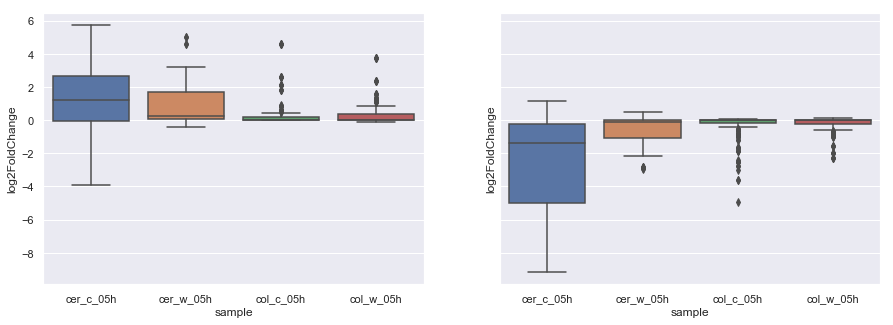
\includegraphics[width=.9\linewidth]{obipy-resources/pairings_05hr_lym_boxplots.png}
\caption{\label{pairings_05hr_lym_boxplots}
Boxplots of differential expressions from 50 largest (left) and 50 lowest (right) DE genes}
\end{figure}


\clearpage\\
\section{lym 6hr c/w}
\label{sec:orgae661e2}

These treatments are comparing the X axis to their lym counter part. e.g. cer\_w is compared to lym\_w and col\_c is compared to lym\_c.\\
\begin{minted}[frame=lines,linenos=true,fontfamily=Monaco]{ipython}
DE_pairings_to_lym_6hr = read_xl('/Users/hughesn/PHD/Transcripts/Data/pairings_to_lym_6hr.xlsx')
\end{minted}


\subsection{Clustermap of largest/smallest DE genes}
\label{sec:orgab5ca0e}

\begin{minted}[frame=lines,linenos=true,fontfamily=Monaco]{ipython}
import matplotlib.pyplot as plt
import seaborn as sns
import numpy as np
%matplotlib inline
top, bot = get_two_clustermaps_data(DE_pairings_to_lym_6hr, 25)
gt = sns.clustermap(top.set_index('gene name'), cmap='bwr', vmin=-10, vmax=10, yticklabels=True, figsize=(20,20))
\end{minted}

\begin{verbatim}
<Figure size 1440x1440 with 4 Axes>
\end{verbatim}


\begin{center}
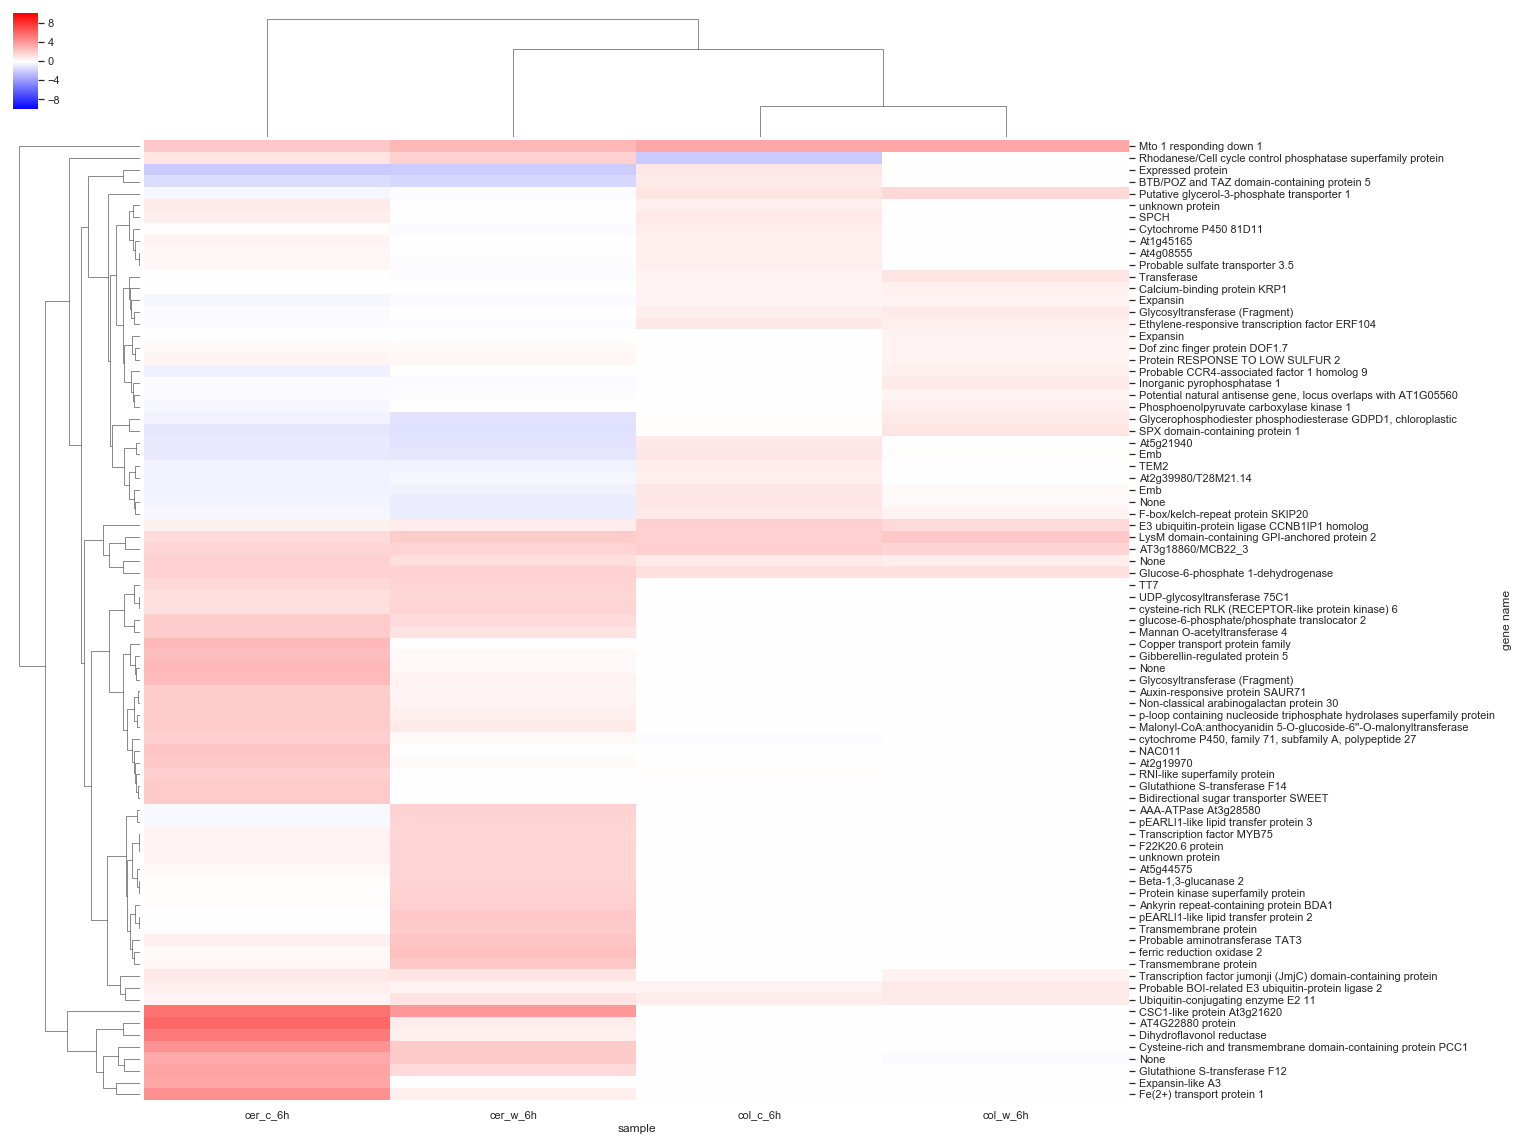
\includegraphics[width=.9\linewidth]{obipy-resources/e77a762dc857123716befe90c8377aaf6f2b9180/75e7de9705fa4a4308f7fb5b627bd547217fec61.png}
\end{center}

\begin{center}
\begin{tabular}{lrrrrl}
gene & cer\_c\_6h & cer\_w\_6h & col\_c\_6h & col\_w\_6h & gene name\\
\hline
AT1G01580 & 0.265538 & 2.43529 & -0.0134848 & 0.000266402 & ferric reduction oxidase 2\\
AT1G05562 & -0.23282 & -0.119374 & 0.0083761 & 0.441658 & Potential natural antisense gene, locus overlaps with AT1G05560\\
AT1G05867 & 1.81801 & 1.32592 & 0.84561 & 0.644058 & None\\
AT1G08650 & -0.339874 & 0.0471269 & 0.00139571 & 0.627517 & Phosphoenolpyruvate carboxylase kinase 1\\
AT1G24147 & 0.356146 & 2.15645 & 0.00122775 & 0.000996686 & Transmembrane protein\\
AT1G24280 & 1.8153 & 1.72072 & 1.18318 & 1.2381 & Glucose-6-phosphate 1-dehydrogenase\\
AT1G32510 & 2.30361 & -0.0436418 & 0.0241369 & -0.00666043 & NAC011\\
AT1G45163 & 0.838653 & -0.0205672 & 0.657192 & 0.00122885 & unknown protein\\
AT1G45165 & 0.503265 & 0.0346636 & 0.652551 & -0.000553874 & At1g45165\\
AT1G49860 & 2.05775 & 0.0327742 & 0.000856933 & 0.0014014 & Glutathione S-transferase F14\\
AT1G51700 & 0.263339 & 0.23231 & 0.000610537 & 0.47405 & Dof zinc finger protein DOF1.7\\
AT1G53480 & 2.13443 & 2.81077 & 3.46707 & 3.4449 & Mto 1 responding down 1\\
AT1G53490 & 0.605604 & 0.7753 & 1.93432 & 1.43818 & E3 ubiquitin-protein ligase CCNB1IP1 homolog\\
AT1G56150 & 1.97823 & 0.449817 & 0.00858026 & 0.0278288 & Auxin-responsive protein SAUR71\\
AT1G56650 & 0.541056 & 1.6369 & -0.00551482 & 0.000388034 & Transcription factor MYB75\\
AT1G61800 & 1.95935 & 1.41486 & -0.00214094 & -0.000158039 & glucose-6-phosphate/phosphate translocator 2\\
AT1G64110 & 2.00061 & 0.688005 & 0.0178664 & 0.000734109 & p-loop containing nucleoside triphosphate hydrolases superfamily protein\\
AT1G68840 & -0.483692 & -0.539192 & 0.724756 & 0.0422114 & TEM2\\
AT1G69530 & -0.359718 & -0.180244 & 0.468465 & 0.544709 & Expansin\\
AT1G73010 & -0.22036 & -0.201325 & 0.00406708 & 0.793724 & Inorganic pyrophosphatase 1\\
AT1G75945 & 3.28769 & 2.08848 & -0.0750018 & -0.160872 & None\\
AT1G76960 & 0.503304 & 1.65842 & -0.00412885 & -0.00554483 & F22K20.6 protein\\
AT1G79110 & 0.645681 & 0.544698 & 0.506675 & 0.880542 & Probable BOI-related E3 ubiquitin-protein ligase 2\\
AT2G17120 & 1.39554 & 1.99613 & 1.8056 & 2.18457 & LysM domain-containing GPI-anchored protein 2\\
AT2G17850 & 1.09006 & 1.85213 & -2.09158 & -0.00437457 & Rhodanese/Cell cycle control phosphatase superfamily protein\\
AT2G19970 & 2.10962 & 0.173878 & 0.00153109 & 0.00401189 & At2g19970\\
AT2G20670 & -2.0612 & -2.00191 & 0.988052 & 0.00472478 & Expressed protein\\
AT2G24850 & 0.622732 & 2.28638 & -0.00618479 & -0.0120888 & Probable aminotransferase TAT3\\
AT2G33790 & 1.98454 & 0.533702 & -0.0102444 & -0.000694328 & Non-classical arabinogalactan protein 30\\
AT2G36800 & -0.212717 & -0.0366492 & 0.663442 & 0.797034 & Glycosyltransferase (Fragment)\\
AT2G39980 & -0.518248 & -0.330112 & 0.668997 & 0.00676105 & At2g39980/T28M21.14\\
AT3G02030 & 0.0376385 & -0.145536 & 0.537838 & 1.02145 & Transferase\\
AT3G02040 & -0.524661 & -1.14136 & 0.117367 & 0.823306 & Glycerophosphodiester phosphodiesterase GDPD1, chloroplastic\\
AT3G02885 & 2.55293 & 0.29424 & -0.00158501 & 0.00505744 & Gibberellin-regulated protein 5\\
AT3G07610 & 0.918947 & 1.08539 & 0.0209842 & 0.546285 & Transcription factor jumonji (JmjC) domain-containing protein\\
AT3G08690 & 0.409444 & 1.14231 & 0.778169 & 0.817438 & Ubiquitin-conjugating enzyme E2 11\\
AT3G09275 & -0.414133 & -0.771378 & 0.942042 & 0.255069 & None\\
AT3G18860 & 1.68638 & 1.71184 & 1.90364 & 1.64174 & AT3g18860/MCB22\_3\\
AT3G21620 & 5.49281 & 4.01802 & 0.000229694 & -0.0189683 & CSC1-like protein At3g21620\\
AT3G22231 & 4.29378 & 2.0807 & 0.000634847 & -0.00662471 & Cysteine-rich and transmembrane domain-containing protein PCC1\\
AT3G28580 & -0.245696 & 1.78259 & -0.00361422 & 5.48356e-05 & AAA-ATPase At3g28580\\
AT3G28740 & 0.0965771 & -0.177175 & 0.774041 & 0.0463688 & Cytochrome P450 81D11\\
AT3G29030 & 0.0602244 & 0.0567001 & 0.00429109 & 0.5358 & Expansin\\
AT3G29590 & 2.02934 & 0.81162 & -0.00137778 & 0.00404867 & Malonyl-CoA:anthocyanidin 5-O-glucoside-6''-O-malonyltransferase\\
AT3G44260 & -0.610296 & -0.0769835 & 0.0509086 & 0.557646 & Probable CCR4-associated factor 1 homolog 9\\
AT3G45960 & 3.47691 & 0.0168601 & 0.0353783 & 0.00783635 & Expansin-like A3\\
AT3G47420 & -0.372151 & -0.124267 & 1.07222 & 1.49742 & Putative glycerol-3-phosphate transporter 1\\
AT3G54160 & 1.92892 & 0.0207161 & 0.0932034 & -0.00634025 & RNI-like superfamily protein\\
AT3G57260 & 0.138099 & 1.68492 & -0.00169744 & -0.00637819 & Beta-1,3-glucanase 2\\
AT3G59940 & -0.389813 & -0.727245 & 0.933464 & 0.472482 & F-box/kelch-repeat protein SKIP20\\
AT4G01080 & 2.01332 & 1.13995 & 0.0104227 & 0.00365152 & Mannan O-acetyltransferase 4\\
AT4G06175 & 2.80322 & 0.305467 & -0.00109173 & 3.23473e-05 & None\\
AT4G08555 & 0.323447 & -0.0767858 & 0.699957 & 0.00411227 & At4g08555\\
AT4G11890 & 0.116206 & 1.75092 & 0.0034015 & -0.00146844 & Protein kinase superfamily protein\\
AT4G12490 & 0.0161937 & 2.13864 & 0.00392383 & 0.00534554 & pEARLI1-like lipid transfer protein 2\\
AT4G12495 & 0.0309393 & 2.07853 & 0.00404906 & 0.00284319 & Transmembrane protein\\
AT4G12500 & -0.284656 & 1.65859 & 0.0359025 & 0.000530587 & pEARLI1-like lipid transfer protein 3\\
AT4G14090 & 1.25833 & 1.63966 & -0.00205242 & 0.0060362 & UDP-glycosyltransferase 75C1\\
AT4G19690 & 4.34839 & 0.679109 & -0.0087742 & 0.000295912 & Fe(2+) transport protein 1\\
AT4G20240 & 1.89957 & 0.262049 & -0.0906711 & -0.015965 & cytochrome P450, family 71, subfamily A, polypeptide 27\\
AT4G22880 & 5.9116 & 0.779074 & -0.00609377 & -0.00130936 & AT4G22880 protein\\
AT4G23140 & 1.30398 & 1.65825 & 0.00361287 & -0.00358306 & cysteine-rich RLK (RECEPTOR-like protein kinase) 6\\
AT4G27280 & 0.0568323 & -0.0214473 & 0.507739 & 0.571907 & Calcium-binding protein KRP1\\
AT4G37610 & -1.40463 & -1.60618 & 0.846049 & 0.0106242 & BTB/POZ and TAZ domain-containing protein 5\\
AT5G07990 & 1.55516 & 1.70322 & 0.000567256 & 0.00162166 & TT7\\
AT5G17220 & 3.59042 & 1.44115 & 0.000302241 & -0.00219097 & Glutathione S-transferase F12\\
AT5G19600 & 0.347219 & -0.112176 & 0.695242 & -0.00426924 & Probable sulfate transporter 3.5\\
AT5G20150 & -0.975805 & -1.24327 & 0.134665 & 1.0524 & SPX domain-containing protein 1\\
AT5G21940 & -0.88004 & -1.11441 & 0.872378 & 0.045652 & At5g21940\\
AT5G24660 & 0.442438 & 0.375215 & 0.00508746 & 0.527337 & Protein RESPONSE TO LOW SULFUR 2\\
AT5G42800 & 5.16998 & 0.614305 & -0.012577 & -0.00095303 & Dihydroflavonol reductase\\
AT5G44575 & 0.270312 & 1.69358 & -0.00332951 & 0.00421994 & At5g44575\\
AT5G44578 & 0.514205 & 1.67249 & 0.00534092 & -0.00172738 & unknown protein\\
AT5G50800 & 2.07154 & -0.0460629 & 0.0129965 & -0.0213864 & Bidirectional sugar transporter SWEET\\
AT5G52710 & 2.77995 & -0.0569704 & 0.0230155 & -0.0172695 & Copper transport protein family\\
AT5G53210 & 0.655746 & 0.0221153 & 0.928035 & 0.00333467 & SPCH\\
AT5G54060 & 2.68115 & 0.469779 & -0.0117165 & -0.00170745 & Glycosyltransferase (Fragment)\\
AT5G54610 & 0.143938 & 1.92923 & 0.000301473 & -0.00119386 & Ankyrin repeat-containing protein BDA1\\
AT5G56550 & -0.930747 & -0.99521 & 0.996667 & 0.145915 & Emb\\
AT5G60680 & -0.470905 & -0.538333 & 0.946323 & 0.300018 & Emb\\
AT5G61600 & -0.199289 & -0.106873 & 0.890552 & 0.693716 & Ethylene-responsive transcription factor ERF104\\
\end{tabular}
\end{center}


\begin{minted}[frame=lines,linenos=true,fontfamily=Monaco]{ipython}
gb = sns.clustermap(bot.set_index('gene name'), cmap='bwr', vmin=-10, vmax=10, yticklabels=True, figsize=(20,20))
\end{minted}

\begin{verbatim}
<Figure size 1440x1440 with 4 Axes>
\end{verbatim}


\begin{center}
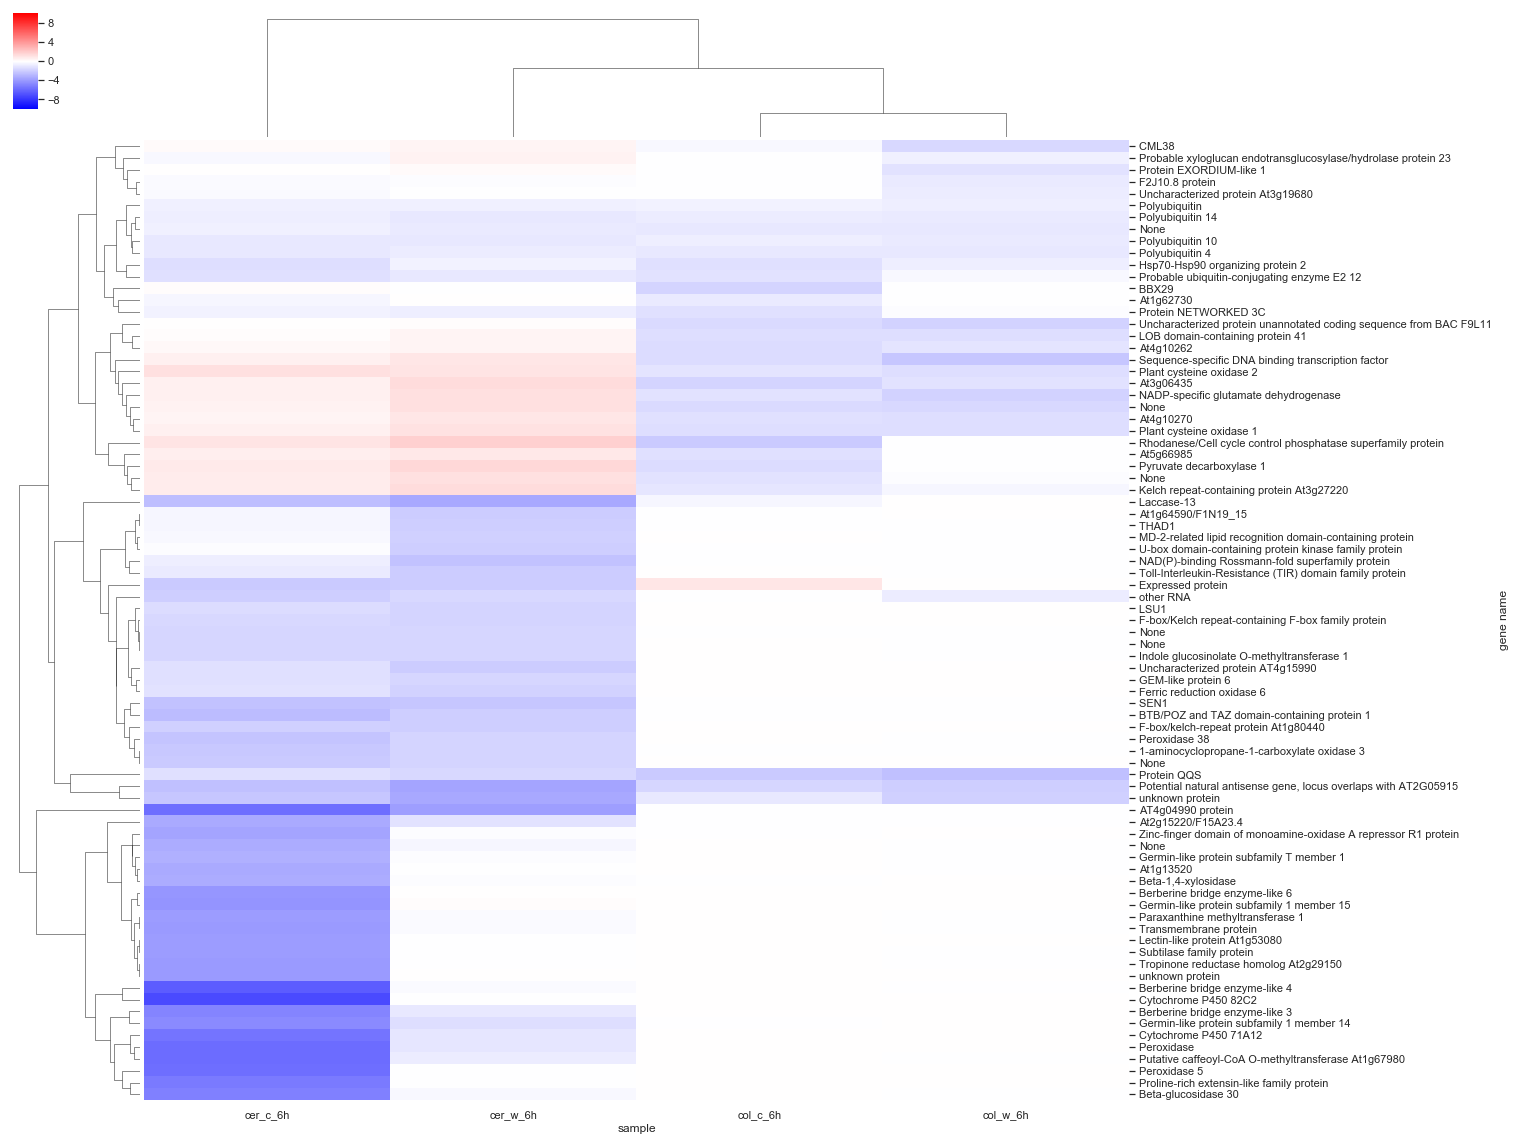
\includegraphics[width=.9\linewidth]{obipy-resources/e77a762dc857123716befe90c8377aaf6f2b9180/d07c120cb3296e04d7ab6270710ee922e4bb528d.png}
\end{center}


\begin{center}
\begin{tabular}{lrrrrl}
gene & cer\_c\_6h & cer\_w\_6h & col\_c\_6h & col\_w\_6h & gene name\\
\hline
AT1G05147 & -1.57087 & -1.62309 & 0.00612245 & -0.00500155 & None\\
AT1G12010 & -2.13351 & -1.67862 & -0.000522444 & -0.00399498 & 1-aminocyclopropane-1-carboxylate oxidase 3\\
AT1G13520 & -3.33802 & -0.0272298 & 0.00169277 & -0.00340154 & At1g13520\\
AT1G14540 & -5.73842 & -0.95748 & 0.000689146 & 0.000779374 & Peroxidase\\
AT1G14550 & -5.69357 & -0.0700701 & 0.00110869 & 0.00523937 & Peroxidase 5\\
AT1G18970 & -3.11141 & -0.0793247 & 7.34396e-05 & -0.00745373 & Germin-like protein subfamily T member 1\\
AT1G21100 & -1.56808 & -1.62372 & 0.00265953 & -0.0042966 & Indole glucosinolate O-methyltransferase 1\\
AT1G23390 & -1.53755 & -1.69403 & 0.017551 & 0.00105973 & F-box/Kelch repeat-containing F-box family protein\\
AT1G26240 & -5.19704 & -0.0140108 & 0.00297997 & 0.00831771 & Proline-rich extensin-like family protein\\
AT1G26380 & -4.78199 & -0.927699 & 0.00385376 & 0.00557304 & Berberine bridge enzyme-like 3\\
AT1G26390 & -6.39275 & -0.179399 & 0.00405959 & -0.00172191 & Berberine bridge enzyme-like 4\\
AT1G26410 & -4.12669 & 0.0259608 & 0.000763462 & 0.00405045 & Berberine bridge enzyme-like 6\\
AT1G33055 & 0.0116033 & 0.154514 & -1.41894 & -1.7281 & Uncharacterized protein unannotated coding sequence from BAC F9L11\\
AT1G35140 & 0.0216269 & 0.213395 & -0.00144094 & -1.09622 & Protein EXORDIUM-like 1\\
AT1G50040 & -0.233111 & -0.104101 & -0.00205244 & -0.849786 & F2J10.8 protein\\
AT1G53080 & -3.84351 & -0.0460042 & 0.00308519 & 0.00133106 & Lectin-like protein At1g53080\\
AT1G62730 & -0.329344 & 0.0358146 & -0.823436 & -0.00164096 & At1g62730\\
AT1G62740 & -1.308 & -0.527233 & -1.23166 & -0.637233 & Hsp70-Hsp90 organizing protein 2\\
AT1G64590 & -0.36541 & -1.96596 & -0.00756918 & 0.00164234 & At1g64590/F1N19\_15\\
AT1G66700 & -3.90245 & -0.208745 & 0.00137037 & -0.00281526 & Paraxanthine methyltransferase 1\\
AT1G66800 & -0.649935 & -2.37502 & -0.00360428 & -0.000485711 & NAD(P)-binding Rossmann-fold superfamily protein\\
AT1G67270 & -3.5176 & -0.0921441 & -0.0146179 & 0.00139016 & Zinc-finger domain of monoamine-oxidase A repressor R1 protein\\
AT1G67980 & -5.76105 & -0.738638 & 0.00867747 & -0.00984984 & Putative caffeoyl-CoA O-methyltransferase At1g67980\\
AT1G76650 & 0.206218 & 0.428762 & -0.301367 & -1.5112 & CML38\\
AT1G80440 & -1.8693 & -1.91855 & 0.0478833 & 0.00066701 & F-box/kelch-repeat protein At1g80440\\
AT2G05914 & -2.45932 & -3.54045 & -1.58399 & -1.91027 & Potential natural antisense gene, locus overlaps with AT2G05915\\
AT2G05915 & -2.22056 & -3.39267 & -0.894739 & -1.80042 & unknown protein\\
AT2G15220 & -3.34358 & -1.16507 & -0.000747652 & -0.00217684 & At2g15220/F15A23.4\\
AT2G17850 & 1.09006 & 1.85213 & -2.09158 & -0.00437457 & Rhodanese/Cell cycle control phosphatase superfamily protein\\
AT2G20670 & -2.0612 & -2.00191 & 0.988052 & 0.00472478 & Expressed protein\\
AT2G25297 & -3.23899 & -0.328027 & 0.00218043 & -0.0103589 & None\\
AT2G29150 & -3.96313 & -0.0199778 & 0.00419643 & -8.42016e-05 & Tropinone reductase homolog At2g29150\\
AT2G30750 & -5.39597 & -0.952528 & 0.00526177 & 0.00228058 & Cytochrome P450 71A12\\
AT2G47920 & -0.545537 & -0.627774 & -1.1807 & -0.0837289 & Protein NETWORKED 3C\\
AT3G02550 & 0.131817 & 0.412505 & -1.30955 & -1.29859 & LOB domain-containing protein 41\\
AT3G06435 & 0.611315 & 1.39065 & -1.71592 & -1.16498 & At3g06435\\
AT3G06436 & 0.714752 & 1.21993 & -1.16212 & -0.109418 & None\\
AT3G08700 & -1.23384 & -0.880382 & -1.1495 & -0.293963 & Probable ubiquitin-conjugating enzyme E2 12\\
AT3G10040 & 0.599268 & 0.995397 & -1.34956 & -2.205 & Sequence-specific DNA binding transcription factor\\
AT3G15635 & -1.60403 & -1.62811 & -0.000289725 & -0.00261783 & None\\
AT3G19615 & -3.25353 & -0.0997206 & -0.00048254 & 5.78413e-05 & Beta-1,4-xylosidase\\
AT3G19680 & -0.188263 & -0.00273222 & -0.037415 & -0.777351 & Uncharacterized protein At3g19680\\
AT3G27220 & 0.762515 & 1.34093 & -1.00252 & -0.345495 & Kelch repeat-containing protein At3g27220\\
AT3G30720 & -1.20203 & -1.49701 & -2.03764 & -2.49854 & Protein QQS\\
AT3G49580 & -1.39022 & -1.64334 & 0.0035161 & 0.000629973 & LSU1\\
AT3G60140 & -4.92355 & -0.242032 & 0.00259034 & -0.00119401 & Beta-glucosidase 30\\
AT4G02890 & -0.671236 & -0.879229 & -0.721226 & -0.813393 & Polyubiquitin 14\\
AT4G04223 & -1.88189 & -1.55083 & -0.00404375 & -0.704525 & other RNA\\
AT4G04335 & -0.582107 & -0.800776 & -0.867402 & -0.873964 & None\\
AT4G04990 & -5.65257 & -3.75659 & -0.00232058 & -0.00224412 & AT4g04990 protein\\
AT4G05050 & -0.55612 & -0.598049 & -0.500152 & -0.667822 & Polyubiquitin\\
AT4G05320 & -0.930702 & -0.861228 & -0.637827 & -0.83074 & Polyubiquitin 10\\
AT4G05775 & 0.537125 & 1.17943 & -1.45021 & -1.50816 & None\\
AT4G08780 & -2.32693 & -1.65501 & 0.00113563 & -0.00262946 & Peroxidase 38\\
AT4G08815 & -2.09289 & -1.66249 & 0.000151272 & 0.000416293 & None\\
AT4G10265 & 0.296372 & 0.419566 & -1.33463 & -1.07547 & At4g10262\\
AT4G10270 & 0.466552 & 0.961928 & -1.21437 & -1.25259 & At4g10270\\
AT4G10530 & -3.8688 & -0.0602774 & 0.00407696 & -0.0102663 & Subtilase family protein\\
AT4G15990 & -1.1995 & -2.0023 & 0.00428221 & 0.00351676 & Uncharacterized protein AT4g15990\\
AT4G19920 & -0.783932 & -2.00754 & 0.000442576 & -0.000961141 & Toll-Interleukin-Resistance (TIR) domain family protein\\
AT4G24110 & 0.611187 & 1.24762 & -1.15071 & -1.78188 & NADP-specific glutamate dehydrogenase\\
AT4G25810 & -0.235847 & 0.519847 & -0.0267727 & -0.623901 & Probable xyloglucan endotransglucosylase/hydrolase protein 23\\
AT4G31970 & -7.04013 & -0.0342645 & 0.00514488 & 0.00749117 & Cytochrome P450 82C2\\
AT4G33070 & 0.80329 & 1.55321 & -1.37282 & -0.0620966 & Pyruvate decarboxylase 1\\
AT4G35770 & -2.38675 & -2.22252 & -0.000784776 & -0.0103655 & SEN1\\
AT4G37290 & -3.92419 & 0.0189886 & 0.00127282 & 0.00665377 & unknown protein\\
AT5G07130 & -2.52585 & -3.38946 & -0.346124 & 0.00171741 & Laccase-13\\
AT5G15120 & 0.624997 & 1.1473 & -1.25493 & -1.31553 & Plant cysteine oxidase 1\\
AT5G20620 & -0.896173 & -0.755113 & -0.888634 & -0.934079 & Polyubiquitin 4\\
AT5G23350 & -1.2016 & -1.626 & 0.0125717 & 0.00551903 & GEM-like protein 6\\
AT5G23840 & -0.26003 & -1.82115 & 0.00161096 & -0.0245467 & MD-2-related lipid recognition domain-containing protein\\
AT5G39110 & -4.55166 & -1.25614 & -0.00160605 & 0.000967537 & Germin-like protein subfamily 1 member 14\\
AT5G39120 & -4.20312 & 0.108445 & 0.00251368 & 0.014211 & Germin-like protein subfamily 1 member 15\\
AT5G39890 & 1.22689 & 1.06626 & -1.08901 & -1.28759 & Plant cysteine oxidase 2\\
AT5G46295 & -3.94342 & -0.232884 & 0.00268564 & -0.000661982 & Transmembrane protein\\
AT5G47990 & -0.348382 & -1.92302 & -0.00919825 & -0.00271743 & THAD1\\
AT5G49730 & -1.11802 & -1.74844 & 0.00168499 & 0.000572037 & Ferric reduction oxidase 6\\
AT5G51270 & -0.152977 & -1.8891 & -0.000121767 & -0.00447423 & U-box domain-containing protein kinase family protein\\
AT5G54470 & 0.101554 & -0.0105956 & -1.68553 & -0.00426739 & BBX29\\
AT5G63160 & -2.58807 & -1.90642 & -0.00432302 & -0.00826455 & BTB/POZ and TAZ domain-containing protein 1\\
AT5G66985 & 0.642771 & 0.876734 & -1.23089 & -0.0253515 & At5g66985\\
\end{tabular}
\end{center}


\subsection{Boxplots of differential changes}
\label{sec:orgaab3217}

\begin{verbatim}
<Figure size 1080x360 with 2 Axes>
\end{verbatim}


\begin{figure}[htbp]
\centering
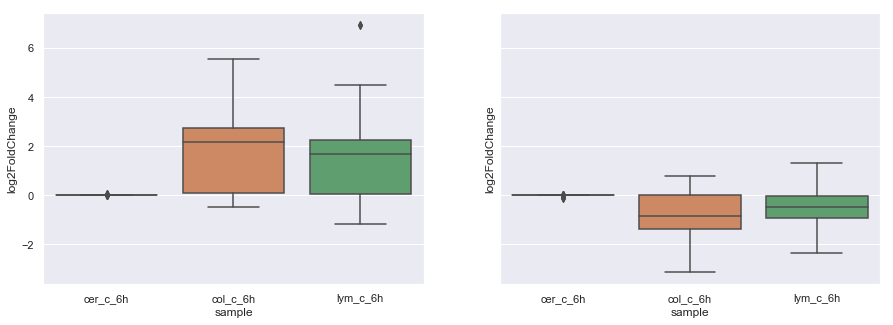
\includegraphics[width=.9\linewidth]{obipy-resources/pairings_6hr_lym_boxplots.png}
\caption{\label{pairings_6hr_lym_boxplots}
Boxplots of differential expressions from 50 largest (left) and 50 lowest (right) DE genes}
\end{figure}


\clearpage\\
\section{all genotypes across time}
\label{sec:org1bd2d46}

Here these figures show the change for each treatment from it's 30min (05hr) to their 6hr counterpart.\\

\begin{minted}[frame=lines,linenos=true,fontfamily=Monaco]{ipython}
DE_cross_time_pairings = read_xl('/Users/hughesn/PHD/Transcripts/Data/cross_time_pairings.xlsx')
\end{minted}


\subsection{Clustermap of largest/smallest DE genes}
\label{sec:org316a0e7}
\begin{minted}[frame=lines,linenos=true,fontfamily=Monaco]{ipython}
import matplotlib.pyplot as plt
import seaborn as sns
import numpy as np
%matplotlib inline
top, bot = get_two_clustermaps_data(DE_cross_time_pairings, 25)
gt = sns.clustermap(top.set_index('gene name'), cmap='bwr', vmin=-10, vmax=10, yticklabels=True, figsize=(20,20))
\end{minted}

\begin{verbatim}
<Figure size 1440x1440 with 4 Axes>
\end{verbatim}


\begin{center}
\includegraphics[width=.9\linewidth]{obipy-resources/e77a762dc857123716befe90c8377aaf6f2b9180/dc6b8763435f3630665e5766345ed659f386df00.png}
\end{center}

\begin{center}
\begin{tabular}{lrrrrrrl}
gene & cer\_c\_05h & cer\_w\_05h & col\_c\_05h & col\_w\_05h & lym\_c\_05h & lym\_w\_05h & gene name\\
\hline
AT1G05767 & 0.131221 & -0.0334292 & 9.1417 & 0 & 9.44474 & 0 & None\\
AT1G06135 & 0.120274 & 0 & 6.85214 & 0.0188751 & 8.02924 & 0 & Transmembrane protein\\
AT1G07135 & 2.24544 & 0.951839 & 5.61576 & 0.984608 & 5.52467 & 1.37907 & At1g07135\\
AT1G07160 & 0.264175 & 0.0010963 & 8.45272 & 0.159339 & 8.38795 & 0.0438174 & PP2C-type phosphatase AP2C2\\
AT1G09950 & 2.34915 & 1.57688 & 5.34701 & 2.78152 & 4.57916 & 1.86987 & At1g09950\\
AT1G12610 & 5.00747 & 2.8787 & 6.78102 & 6.91874 & 7.27127 & 5.00418 & Dehydration-responsive element-binding protein 1F\\
AT1G14540 & 2.89502 & 0.407181 & 4.56608 & -0.00241023 & 4.92331 & 0.112505 & Peroxidase\\
AT1G15010 & 1.7376 & 2.05528 & 3.16298 & 0.554411 & 3.22936 & 0.134466 & Mediator of RNA polymerase II transcription subunit\\
AT1G17345 & 0.312913 & 1.80323 & -0.243988 & 0.0455167 & -0.163458 & 0.201671 & Auxin-responsive protein SAUR77\\
AT1G18300 & 1.93989 & 1.62098 & 4.55968 & 1.17499 & 4.5911 & 0.667534 & Nudix hydrolase 4\\
AT1G20310 & 1.30842 & 0.0831904 & 8.39919 & 0.0648718 & 6.56573 & -0.0317942 & Syringolide-induced protein\\
AT1G27730 & 2.23589 & 1.10252 & 5.10695 & 0.294588 & 5.21002 & 0.854413 & Zinc finger protein ZAT10\\
AT1G33055 & 0.000810339 & 0.0154475 & 2.15222 & 3.10392 & 0.267653 & 1.03591 & Uncharacterized protein unannotated coding sequence from BAC F9L11\\
AT1G33760 & 1.75486 & 0.910781 & 4.43209 & 2.88909 & 4.94529 & 1.15473 & Ethylene-responsive transcription factor ERF022\\
AT1G35140 & 1.7375 & 0.933701 & 5.05985 & 3.05073 & 4.65205 & 1.38493 & Protein EXORDIUM-like 1\\
AT1G43000 & 0.781076 & 0.0995261 & 8.42032 & -0.0392258 & 7.55239 & 1.32167 & PLATZ transcription factor family protein\\
AT1G43800 & 1.96003 & 2.34598 & 2.22853 & 1.81907 & 2.62515 & 3.18352 & Stearoyl-\\
AT1G47130 & 0.215106 & 0.0607207 & 5.92014 & 0.0385085 & 8.43442 & 0.144643 & None\\
AT1G55430 & 0.582111 & 1.74325 & 1.95957 & 1.81612 & 1.27926 & 0.0443272 & Cysteine/Histidine-rich C1 domain family protein\\
AT1G56240 & 1.72051 & 0.0990209 & 8.05145 & 0.149415 & 8.39011 & 0.100802 & F-box protein PP2-B13\\
AT1G56242 & 0.802021 & 0.00293639 & 7.97256 & 0.0365258 & 8.64022 & 0.205246 & other RNA\\
AT1G56250 & 3.37139 & 0.0507228 & 8.39725 & 0.115112 & 7.69363 & 0.0964437 & F-box protein VBF\\
AT1G63030 & 4.09911 & 0.992102 & 5.64752 & 4.20864 & 6.17599 & 2.67556 & Dehydration-responsive element-binding protein 1E\\
AT1G66090 & 1.60555 & 0.135117 & 6.86201 & 0.324025 & 7.38427 & 1.78461 & Disease resistance protein (TIR-NBS class)\\
AT1G72540 & 0.0511969 & 1.59265 & 1.49675 & 0.0415312 & 1.43385 & 0.352027 & Putative receptor-like protein kinase At1g72540\\
AT1G73010 & 1.46593 & 1.6423 & 1.18193 & -0.711766 & 1.87748 & 0.879309 & Inorganic pyrophosphatase 1\\
AT1G76650 & 1.46113 & 0.59485 & 4.25121 & 3.24354 & 3.39952 & 1.20674 & CML38\\
AT1G77640 & 1.24714 & 2.92898 & 3.29079 & 1.45327 & 2.8383 & 1.83868 & Ethylene-responsive transcription factor ERF013\\
AT2G17660 & 2.54253 & 0.226289 & 5.44864 & 4.49545 & 3.50637 & 1.046 & At2g17660\\
AT2G17845 & 0.31046 & 0.230546 & 4.01346 & 4.83504 & 3.23005 & 3.47902 & NAD(P)-binding Rossmann-fold superfamily protein\\
AT2G17850 & 0.762908 & 1.05679 & 4.68448 & 3.93859 & 2.32643 & 3.76101 & Rhodanese/Cell cycle control phosphatase superfamily protein\\
AT2G21200 & -0.119127 & -0.0140999 & 0.102829 & 3.56975 & -1.52344 & 0.191833 & At2g21200\\
AT2G22760 & 1.55059 & 0.0737552 & 7.12523 & 0.490295 & 7.19557 & 0.376071 & Uncharacterized protein At2g22760 (Fragment)\\
AT2G25460 & 2.60721 & 3.20012 & 5.07223 & 2.34301 & 5.41635 & 1.33195 & CONTAINS InterPro DOMAIN/s: C2 calcium-dependent membrane targeting (InterPro:IPR000008)\\
AT2G26400 & 1.91194 & 1.48305 & 1.83636 & 0.030103 & 2.06658 & 2.24961 & acireductone dioxygenase 3\\
AT2G29110 & 0.025719 & 0.0354131 & 7.02538 & 0.0199806 & 6.46903 & 0.138044 & Glutamate receptor\\
AT2G31345 & 0.0261995 & 0.0249383 & 8.82703 & -0.0190216 & 7.97938 & -0.0277433 & Transmembrane protein\\
AT2G34600 & 2.14154 & 0.787817 & 2.58479 & 1.96543 & 1.5903 & 1.6744 & Protein TIFY 5B\\
AT2G35290 & 2.3177 & 0.0722224 & 2.47513 & 1.66998 & 1.80411 & 1.68675 & At2g35290\\
AT2G36440 & 0 & 0.00146419 & 7.36923 & 0.0183288 & 7.33671 & -0.130565 & Uncharacterized protein At2g36440\\
AT2G37430 & 1.40793 & 0.0484521 & 7.49643 & 0.0675307 & 8.15927 & 0.263368 & ZAT11\\
AT2G44840 & 2.31768 & 1.28108 & 6.80366 & 0.0767919 & 7.65875 & 1.20029 & Ethylene-responsive transcription factor 13\\
AT2G46400 & 2.51447 & 1.79201 & 5.73995 & 1.26039 & 5.79294 & 1.71659 & Probable WRKY transcription factor 46\\
AT2G47520 & 0.604806 & 0.881384 & 4.01626 & 2.2069 & 2.80491 & 2.24381 & Ethylene-responsive transcription factor ERF071\\
AT3G01055 & 1.19886 & 0.183933 & 6.41978 & 0.582986 & 7.80493 & 0.512532 & None\\
AT3G01165 & 1.75902 & 0.282712 & 9.27442 & 0.00996791 & 8.32328 & 0.0541064 & None\\
AT3G02840 & 0.333485 & 0.103235 & 8.45014 & 0.336227 & 9.05894 & 0.359589 & ARM repeat superfamily protein\\
AT3G06435 & 0.00791533 & 0.0684112 & 2.31893 & 3.51549 & 0.176069 & 1.76157 & At3g06435\\
AT3G06436 & 0.0298105 & 0.0555049 & 1.69647 & 2.34982 & 0.357944 & 1.86961 & None\\
AT3G10040 & -0.0568406 & -0.0563251 & 2.09916 & 3.76502 & 0.285153 & 1.04781 & Sequence-specific DNA binding transcription factor\\
AT3G14260 & 2.26044 & 0.0349616 & 0.178845 & -0.00601058 & -0.0127085 & 0.0525859 & Protein LURP-one-related 11\\
AT3G16860 & 2.20979 & 1.4295 & 3.13451 & 2.32599 & 3.85719 & 1.51066 & COBRA-like protein 8\\
AT3G21150 & 0.316924 & 0.0145792 & 6.8125 & 0.0366141 & 7.49146 & 0.475475 & B-box zinc finger protein 32\\
AT3G27220 & 0.0909242 & 0.501585 & 1.75426 & 2.62113 & 0.733802 & 1.95118 & Kelch repeat-containing protein At3g27220\\
AT3G29000 & 1.57076 & 0.191746 & 7.30764 & 0.020447 & 6.8332 & 0.469843 & Probable calcium-binding protein CML45\\
AT3G45960 & 2.08478 & 2.84037 & 5.05602 & 0.728454 & 8.05484 & 2.57457 & Expansin-like A3\\
AT3G47720 & 0.0202986 & 0.00674602 & 3.05648 & 3.97859 & 0.957408 & 2.79075 & Probable inactive poly\\
AT3G48520 & 2.53982 & 2.33525 & 2.38797 & 3.61556 & 1.97295 & 2.36675 & CYP94B3\\
AT3G56790 & 0.000390123 & 0.105644 & 8.05951 & -0.0725291 & 7.99565 & 0.0916867 & RNA splicing factor-like protein\\
AT4G01360 & 2.79733 & 0.902955 & 5.88313 & 3.15754 & 4.50768 & 2.43205 & BPS1-like protein\\
AT4G04480 & -0.0832397 & 0 & 7.88243 & 0 & 8.24819 & 0 & F-box protein with a domain protein\\
AT4G05775 & 0.0188596 & 0.0291996 & 2.22961 & 3.29526 & 0.260435 & 1.3221 & None\\
AT4G08040 & 0.490898 & 0.605692 & 3.0356 & 2.55037 & 1.68729 & 1.96469 & 1-aminocyclopropane-1-carboxylate synthase 11\\
AT4G08985 & 5.31255 & 3.53629 & 8.0185 & 4.32632 & 7.5748 & 4.84115 & None\\
AT4G10265 & -0.0924162 & -0.0650159 & 2.21601 & 2.86452 & 0.108844 & 0.604047 & At4g10262\\
AT4G21840 & 2.20349 & 0.785653 & 3.29048 & 1.19698 & 2.50268 & 1.65373 & MSRB8\\
AT4G22030 & 0.0161654 & 0.0115561 & 8.11585 & 0 & 7.03238 & 0 & F-box family protein with a domain of unknown function (DUF295)\\
AT4G24110 & 0.241401 & 0.0888118 & 4.04646 & 3.68591 & 2.76444 & 1.48434 & NADP-specific glutamate dehydrogenase\\
AT4G24570 & 2.3828 & 1.46625 & 6.06616 & 1.01442 & 6.87497 & 1.63194 & DIC2\\
AT4G27652 & 2.02696 & 1.6986 & 2.54029 & 0.700608 & 2.89759 & 1.30719 & At4g27652\\
AT4G27654 & 6.26622 & 3.71037 & 7.92796 & 4.9031 & 7.68114 & 4.52447 & At4g27654\\
AT4G29780 & 2.31501 & 1.96174 & 6.36144 & 0.89414 & 6.59436 & 1.55332 & Nuclease\\
AT4G31950 & 0.095676 & -0.00823225 & 9.84324 & 0.00352272 & 10.0663 & 0.0216446 & CYP82C3\\
AT4G33070 & 1.42573 & 1.49719 & 3.73558 & 3.82909 & 2.39907 & 3.20531 & Pyruvate decarboxylase 1\\
AT4G33560 & 0.721302 & 0.666798 & 1.64427 & 1.94182 & 1.03609 & 1.77793 & At4g33560\\
AT5G02200 & 0.161875 & 0.268325 & 2.59416 & 0.795523 & 1.6851 & 2.60969 & Protein FAR-RED-ELONGATED HYPOCOTYL 1-LIKE\\
AT5G05300 & 1.148 & -0.0245958 & 6.75565 & -0.00917287 & 7.40462 & 0.0823586 & Gb\\
AT5G10040 & 1.23241 & 1.60107 & 3.74562 & 3.85759 & 1.64716 & 3.70768 & At5g10040\\
AT5G11140 & 0.136151 & 0.0116309 & 7.67926 & -0.0845706 & 9.1037 & 0.0364596 & Phospholipase-like protein (PEARLI 4) family protein\\
AT5G15120 & 0.0840484 & 0.163887 & 2.59628 & 3.26334 & 1.25272 & 1.53051 & Plant cysteine oxidase 1\\
AT5G17350 & 2.67389 & 1.87667 & 5.74493 & 1.48953 & 4.97885 & 1.3327 & Uncharacterized protein At5g17350\\
AT5G20150 & 1.2761 & 1.6311 & -0.88117 & -1.2489 & 0.445263 & 0.610701 & SPX domain-containing protein 1\\
AT5G24110 & 0.0416349 & 0.57146 & 7.79825 & 0.118043 & 8.51506 & 0.112671 & Probable WRKY transcription factor 30\\
AT5G39890 & 0.214771 & 0.539333 & 2.97013 & 3.70325 & 1.63539 & 2.08617 & Plant cysteine oxidase 2\\
AT5G42380 & 3.15032 & 0.585206 & 7.47516 & 0.152636 & 7.4884 & 0.361152 & Calcium-binding protein CML37\\
AT5G46500 & 0.613513 & 1.83163 & 3.68489 & 1.67886 & 4.15509 & 1.9397 & Protein VARIATION IN COMPOUND TRIGGERED ROOT growth protein\\
AT5G47850 & 0.0048455 & 0.00938611 & 9.22619 & -0.00844845 & 7.10715 & 0.0790617 & Serine/threonine-protein kinase-like protein CCR4\\
AT5G52020 & 2.68309 & 3.37151 & 3.55615 & 3.20815 & 2.67236 & 1.48473 & Ethylene-responsive transcription factor ERF025\\
AT5G52710 & 1.13267 & 1.73556 & 5.24241 & 0.736045 & 7.00402 & 0.109046 & Copper transport protein family\\
AT5G57010 & 1.96161 & 1.80542 & 4.62157 & 0.0615569 & 4.01027 & 1.22528 & IQ domain-containing protein IQM5\\
AT5G66640 & 2.08912 & 1.80585 & 4.2288 & 0.0698819 & 5.19871 & 0.870108 & DA1-related protein 3\\
\end{tabular}
\end{center}


\begin{minted}[frame=lines,linenos=true,fontfamily=Monaco]{ipython}
gb = sns.clustermap(bot.set_index('gene name'), cmap='bwr', vmin=-10, vmax=10, yticklabels=True, figsize=(20,20))
\end{minted}

\begin{verbatim}
<Figure size 1440x1440 with 4 Axes>
\end{verbatim}


\begin{center}
\includegraphics[width=.9\linewidth]{obipy-resources/e77a762dc857123716befe90c8377aaf6f2b9180/afa7394d08540e5751a8d74b94e3d55fe91bf815.png}
\end{center}


\begin{center}
\begin{tabular}{lrrrrrrl}
gene & cer\_c\_05h & cer\_w\_05h & col\_c\_05h & col\_w\_05h & lym\_c\_05h & lym\_w\_05h & gene name\\
\hline
AT1G03850 & -1.38926 & -0.735956 & -1.11439 & -0.0320717 & -1.71162 & -0.354113 & Glutaredoxin family protein\\
AT1G04770 & -1.05908 & -1.22307 & -1.69706 & 0.00681842 & -1.97311 & -0.479349 & Protein SULFUR DEFICIENCY-INDUCED 2\\
AT1G05560 & -0.413218 & -0.925634 & -1.1031 & -1.50316 & -1.01678 & -1.2646 & UDP-glucosyltransferase 75B1\\
AT1G05562 & -0.388962 & -1.00075 & -0.81255 & -1.5777 & -0.932614 & -1.08226 & Potential natural antisense gene, locus overlaps with AT1G05560\\
AT1G06160 & -0.00246996 & -0.0227016 & -2.28419 & -0.301198 & -2.84134 & -0.429338 & Ethylene-responsive transcription factor ERF094\\
AT1G06980 & -0.0294207 & -0.0399044 & -3.5452 & -0.000552876 & -0.704986 & -0.022073 & 6,7-dimethyl-8-ribityllumazine synthase\\
AT1G10585 & -0.433824 & -1.00684 & -1.21368 & -0.258704 & -1.81604 & -1.28804 & Transcription factor bHLH167\\
AT1G12740 & -1.18777 & -0.140889 & 0.0759523 & -0.0770483 & -0.208367 & -0.345759 & Cytochrome P450, family 87, subfamily A, polypeptide 2\\
AT1G13245 & -0.0684023 & -0.0632047 & -2.84557 & -0.835528 & -1.47898 & -0.850327 & At1g13245\\
AT1G14860 & -0.49175 & -1.01277 & -0.276527 & -0.118403 & -0.201791 & -0.356167 & Nudix hydrolase 18, mitochondrial\\
AT1G18350 & -0.0328392 & 0.0150336 & -0.198993 & -0.065007 & -2.87613 & -0.875448 & MKK7\\
AT1G19620 & -0.0530932 & -0.0229593 & -3.06276 & 0.0333328 & -0.360107 & -0.0308265 & unknown protein\\
AT1G23052 & -0.455399 & -0.0144443 & -3.15399 & -0.152663 & -0.406051 & -0.276443 & None\\
AT1G23390 & -1.13611 & -0.714682 & -2.69743 & -1.80246 & -2.4545 & -2.11807 & F-box/Kelch repeat-containing F-box family protein\\
AT1G26390 & 0.0135578 & -0.00161186 & -1.99848 & 0.039604 & -3.16721 & -0.00133306 & Berberine bridge enzyme-like 4\\
AT1G26800 & -0.930127 & -0.591443 & -2.63846 & -0.542997 & -2.44157 & -1.70746 & E3 ubiquitin-protein ligase MPSR1\\
AT1G31173 & -0.0139765 & 0.00043779 & -3.28846 & 0.043577 & -6.87794 & -0.105809 & MIR167D\\
AT1G49130 & -1.39398 & -0.0547904 & -1.91239 & -1.18475 & -1.61724 & -1.19133 & B-box type zinc finger protein with CCT domain-containing protein\\
AT1G49200 & -0.987098 & -0.0458262 & -3.97399 & -0.772236 & -4.20861 & -0.991139 & RING-H2 finger protein ATL75\\
AT1G49205 & -0.253514 & -0.0654313 & -4.252 & -1.18486 & -4.46302 & -0.185123 & None\\
AT1G49310 & -1.29303 & -0.017745 & -0.03177 & 0.0265248 & -0.0323654 & -0.0283561 & At1g49310\\
AT1G49500 & -1.48917 & -0.778099 & -1.37059 & -0.813168 & -1.46752 & -1.43432 & At1g49500/F13F21\_6\\
AT1G49640 & -0.0849337 & -0.106878 & -2.86686 & -0.236768 & -1.90204 & -0.160104 & Probable carboxylesterase 3\\
AT1G52342 & -0.0385584 & -0.538964 & -0.478502 & -0.161346 & -0.843369 & -2.2434 & Putative uncharacterized protein\\
AT1G68190 & -0.455311 & -1.15125 & -0.30066 & -0.075555 & -0.620373 & -1.40924 & B-box zinc finger family protein\\
AT1G69490 & 0.0446486 & -0.0384023 & -2.06739 & -0.672257 & -0.874696 & -1.61403 & NAP\\
AT1G71030 & -0.724194 & -0.0123642 & -1.82912 & -2.6498 & -1.26043 & -2.09671 & At1g71030/F23N20\_2\\
AT1G73830 & -0.996345 & -0.750874 & -2.10194 & -0.877105 & -2.46929 & -1.62769 & Transcription factor BEE 3\\
AT1G75380 & -1.06467 & -1.04874 & -1.23928 & -0.20493 & -1.17532 & -1.00129 & Bifunctional nuclease 1\\
AT1G80440 & -1.23835 & -1.06885 & -2.52565 & -2.01958 & -2.49577 & -2.91705 & F-box/kelch-repeat protein At1g80440\\
AT2G05070 & -1.14202 & -0.509099 & -0.078545 & -0.342325 & -0.320514 & -0.667058 & Chlorophyll a-b binding protein 2.2, chloroplastic\\
AT2G05100 & -1.17507 & -0.588801 & -0.174089 & -0.14865 & -0.250942 & -0.480003 & photosystem II light harvesting complex gene 2.1\\
AT2G20670 & -0.152435 & -0.631439 & -2.66891 & -2.28262 & -1.59127 & -2.29484 & Expressed protein\\
AT2G25900 & -0.0993798 & -1.23561 & -0.820886 & -0.61028 & -0.0446706 & -0.995928 & Zinc finger CCCH domain-containing protein 23\\
AT2G27830 & -0.0654508 & -0.466908 & 0.520546 & -1.06302 & 1.26543 & -1.63375 & Expressed protein\\
AT2G29300 & -1.91636 & -0.116147 & -0.909031 & -0.000715312 & -1.42893 & -0.0900465 & NAD(P)-binding Rossmann-fold superfamily protein\\
AT2G29460 & -0.0191687 & -1.02589 & -0.793983 & -0.513134 & -1.2596 & -1.58614 & Glutathione S-transferase U4\\
AT2G30750 & 0.00417857 & 0.00495212 & -3.16133 & -0.0433873 & -3.42763 & -0.206335 & Cytochrome P450 71A12\\
AT2G36750 & -0.13356 & -0.496012 & -1.60357 & -1.45319 & -3.0624 & -1.39302 & UDP-glycosyltransferase 73C1\\
AT2G36800 & -0.00926727 & -1.0309 & -0.806129 & -1.9669 & -0.236542 & -1.1498 & Glycosyltransferase (Fragment)\\
AT2G37750 & -0.969029 & -1.14072 & -1.70391 & -0.044768 & -1.98638 & -1.24342 & Expressed protein\\
AT2G39380 & -1.15897 & -0.243813 & 1.33913 & -0.268517 & 0.124042 & -0.17754 & Exocyst subunit Exo70 family protein\\
AT2G39400 & -0.416317 & -0.581706 & 0.82437 & -0.443286 & 0.532221 & -1.57936 & Alpha/beta-Hydrolases superfamily protein\\
AT3G02040 & 0.556009 & 0.803486 & -0.644491 & -1.58176 & 0.19269 & 0.0416792 & Glycerophosphodiester phosphodiesterase GDPD1, chloroplastic\\
AT3G04060 & -0.00292222 & -0.0215771 & -0.580251 & -0.0224993 & -0.338069 & -1.63587 & NAC domain-containing protein 46\\
AT3G04530 & -0.0934097 & -0.210195 & -2.00562 & -0.0787853 & -3.61561 & -0.939369 & Phosphoenolpyruvate carboxylase kinase 2\\
AT3G04685 & -0.386395 & -1.24423 & -1.55949 & -0.255984 & -0.760232 & -0.0712309 & None\\
AT3G06390 & -1.47222 & -0.362403 & 0.256486 & 0.021042 & -0.0177879 & -0.489815 & CASP-like protein 1D2\\
AT3G07350 & -0.0721898 & -0.30885 & -1.89528 & -1.82333 & -1.16807 & -1.49448 & F21O3.6 protein\\
AT3G08860 & -0.480164 & -1.52246 & -0.269586 & -0.0116631 & -0.388823 & -1.17216 & Alanine--glyoxylate aminotransferase 2 homolog 3, mitochondrial\\
AT3G09275 & -1.12876 & -0.746403 & -4.29317 & -1.39865 & -3.28358 & -1.21037 & None\\
AT3G09415 & -1.15064 & -1.03445 & -0.0267187 & -0.119232 & 0.0804321 & -0.089331 & None\\
AT3G15450 & -1.03687 & -1.48958 & -0.501557 & -0.0642759 & -1.0515 & -1.52418 & AT3g15450/MJK13\_11\\
AT3G15500 & 0.00074855 & -0.0523677 & -2.15058 & -1.41615 & -0.879842 & -1.3984 & NAC3\\
AT3G18773 & -0.0348841 & -0.0085592 & -2.04077 & -1.63241 & -0.416067 & -1.58183 & RING-H2 finger protein ATL77\\
AT3G21500 & -0.0564114 & -0.0456016 & -0.133283 & -0.017052 & -3.21375 & -0.0580272 & 1-deoxy-D-xylulose 5-phosphate synthase 1\\
AT3G26510 & -0.000816748 & -0.0452865 & -2.32707 & -1.61949 & -1.40685 & -1.27282 & Octicosapeptide/Phox/Bem1p family protein\\
AT3G26512 & -0.0132985 & -0.0353256 & -2.29974 & -1.65924 & -1.72362 & -1.19681 & None\\
AT3G28740 & -2.60709 & -4.25397 & -2.3867 & -3.37829 & -1.25526 & -5.084 & Cytochrome P450 81D11\\
AT3G29035 & -1.57362 & -0.945074 & -1.30669 & -0.768348 & -1.03506 & -1.75779 & NAC domain-containing protein 59\\
AT3G47420 & 1.50697 & 1.17881 & -1.65203 & -1.54148 & -0.0772408 & 0.775197 & Putative glycerol-3-phosphate transporter 1\\
AT3G48360 & -1.43644 & -1.15649 & -0.474331 & -0.626644 & -0.768862 & -1.17738 & BTB/POZ and TAZ domain-containing protein 2\\
AT3G49790 & -0.135422 & -0.216708 & -0.155095 & -0.389992 & -0.116694 & -1.63743 & At3g49790\\
AT3G50310 & -0.0691382 & -0.160397 & -3.42123 & -0.0460974 & -3.35719 & -0.091952 & MKKK20\\
AT3G50770 & -0.0519309 & 0.019146 & -1.72479 & -1.42212 & -0.858292 & -1.42581 & Probable calcium-binding protein CML41\\
AT3G53150 & -1.58592 & 0.000147762 & 0.0524943 & -0.022729 & 0.0685967 & -0.0242104 & UDP-glucosyl transferase 73D1\\
AT3G59940 & -1.06419 & -0.969801 & -4.02533 & -1.27922 & -2.92047 & -1.14996 & F-box/kelch-repeat protein SKIP20\\
AT3G60140 & 0.0151218 & -0.0268673 & -3.76862 & -0.0554408 & -5.44865 & -0.242466 & Beta-glucosidase 30\\
AT3G62950 & -0.0378661 & -0.0343968 & -4.48917 & -0.095595 & -0.830458 & -0.403051 & Glutaredoxin-C11\\
AT3G63210 & -1.59696 & -1.2564 & -1.39764 & -0.73242 & -1.66535 & -1.17749 & Protein MARD1\\
AT4G08555 & 0.190242 & 0.0222866 & 2.34568 & -1.72007 & 4.44439 & -0.420745 & At4g08555\\
AT4G12500 & -0.224588 & -0.029061 & -4.23952 & -0.0102156 & -3.43277 & -0.9901 & pEARLI1-like lipid transfer protein 3\\
AT4G15660 & -0.0631508 & -0.0691569 & -2.98388 & -1.47989 & -1.53434 & -0.77992 & Monothiol glutaredoxin-S8\\
AT4G15670 & -0.300925 & -0.0207581 & -2.02228 & -1.77038 & -1.12408 & -1.20167 & Monothiol glutaredoxin-S7\\
AT4G15680 & -0.380275 & -0.10453 & -2.16372 & -1.51484 & -1.96735 & -0.876141 & Monothiol glutaredoxin-S4\\
AT4G15690 & -0.94959 & -0.0257734 & -1.52399 & -1.49374 & -0.694211 & -1.25328 & Monothiol glutaredoxin-S5\\
AT4G15765 & -1.18389 & -0.0234651 & -0.241851 & -0.0531795 & -0.357872 & -0.244407 & FAD/NAD(P)-binding oxidoreductase family protein\\
AT4G18630 & -0.110712 & -0.00177774 & -1.05724 & -1.80996 & -0.150503 & -0.0507635 & Uncharacterized protein At4g18630/F28A21\_40\\
AT4G19170 & -0.0759198 & -0.04171 & -2.41256 & -1.22117 & -1.61784 & -1.54598 & Probable carotenoid cleavage dioxygenase 4, chloroplastic\\
AT4G19700 & 0.0886102 & 0.0630215 & -2.92355 & -0.0211871 & -2.71428 & 0.0426638 & E3 ubiquitin-protein ligase BOI\\
AT4G20450 & -0.0454526 & -0.00474583 & -0.140622 & -0.00112377 & 0.019423 & -1.53875 & Probable LRR receptor-like serine/threonine-protein kinase At4g20450\\
AT4G21990 & -0.788526 & -1.06071 & -0.705096 & -1.02215 & -0.915621 & -1.07295 & 5'-adenylylsulfate reductase 3, chloroplastic\\
AT4G23700 & -0.322015 & -0.797532 & -1.18922 & -0.0458442 & -1.63559 & -1.76268 & Cation/H(+) antiporter 17\\
AT4G25220 & -0.0252709 & 0.00893559 & 1.38667 & 0.0312999 & 1.01403 & -1.84802 & Putative glycerol-3-phosphate transporter 2\\
AT4G31970 & -0.025132 & 0 & -5.69798 & -0.00684202 & -6.88759 & -0.0275751 & Cytochrome P450 82C2\\
AT4G34135 & 0.0840303 & -0.0265266 & -0.759695 & -1.45482 & -0.544967 & -0.819114 & UDP-glucosyl transferase 73B2\\
AT4G34250 & -1.20735 & -0.168863 & -1.4129 & -0.0509559 & -0.658219 & -0.554335 & 3-ketoacyl-CoA synthase 16\\
AT4G35720 & -0.0164758 & -0.0414955 & -3.68457 & -0.201543 & -1.40231 & -0.0966743 & DUF241 domain protein, putative (DUF241)\\
AT4G36040 & -0.285431 & -0.38231 & -2.34086 & -1.1746 & -2.09115 & -1.59484 & At4g36040\\
AT4G37990 & -0.0359532 & -0.0388621 & -0.228074 & -0.272828 & -4.26807 & -0.245371 & Cinnamyl alcohol dehydrogenase 8\\
AT4G38850 & 0.0393783 & 0.00896711 & -0.0996547 & 0.106719 & -3.8893 & 0.0479883 & Auxin-responsive protein SAUR15\\
AT5G00855 & -0.0164819 & -0.0537079 & -0.143818 & -0.141641 & -3.65752 & -0.00870306 & None\\
AT5G06980 & -0.930808 & -1.31918 & -0.0707946 & -0.074441 & -0.404033 & -0.617522 & unknown protein\\
AT5G10990 & -0.579777 & -0.0265981 & -0.668724 & -0.030518 & -3.94236 & -0.0852426 & At5g10990\\
AT5G22920 & -1.60905 & -1.44508 & -0.74071 & -0.164183 & -1.46598 & -1.63446 & E3 ubiquitin-protein ligase RZFP34\\
AT5G25130 & -1.39073 & -0.119904 & -0.196733 & -0.00838264 & -0.339129 & -0.226474 & Cytochrome P450 71B12\\
AT5G25280 & -0.243009 & -0.0291201 & -2.84467 & -0.977576 & -2.62003 & -0.849764 & AT5g25280/F18G18\_20\\
AT5G26290 & -0.841253 & -1.00882 & 0.063839 & -0.0312998 & -0.984636 & -0.290765 & TRAF-like family protein\\
AT5G39120 & -0.0054049 & -0.0703556 & -3.98686 & 0.00539812 & -4.07454 & -0.00831133 & Germin-like protein subfamily 1 member 15\\
AT5G39130 & -0.0126127 & -0.0304824 & -3.4883 & 0.0110587 & -1.47682 & 0.0065836 & Germin-like protein subfamily 1 member 16\\
AT5G39610 & -0.277444 & -0.740002 & -2.02708 & -0.633264 & -1.62727 & -1.56969 & NAC domain-containing protein 92\\
AT5G43540 & -0.0332622 & 0.00333862 & -1.60684 & -0.0160477 & -2.95759 & -0.133047 & C2H2 and C2HC zinc fingers superfamily protein\\
AT5G44260 & -0.740388 & -0.192349 & -1.78498 & -1.19188 & -1.9699 & -1.84684 & Zinc finger CCCH domain-containing protein 61\\
AT5G45820 & -1.976 & -1.82637 & -1.80459 & -0.124983 & -0.836874 & -1.3218 & CBL-interacting serine/threonine-protein kinase 20\\
AT5G45830 & -0.198316 & -0.215055 & -0.295949 & -0.201634 & -3.18721 & -0.777364 & delay of germination 1\\
AT5G49360 & -1.34403 & -1.09472 & -0.118198 & 0.0293375 & -0.337928 & -0.744066 & Beta-D-xylosidase 1\\
AT5G52900 & -0.0893949 & -0.00582752 & -3.0471 & -0.748934 & -2.74757 & -0.118708 & Probable membrane-associated kinase regulator 6\\
AT5G53980 & -0.475419 & -0.0860896 & -2.5215 & -1.64736 & -2.88505 & -0.820739 & Homeobox-leucine zipper protein ATHB-52\\
AT5G57660 & -1.4987 & -0.916936 & -1.14611 & -0.819935 & -1.39278 & -1.19347 & Zinc finger protein CONSTANS-LIKE 5\\
AT5G59220 & -0.0202128 & -1.08436 & 0.113852 & -0.0553742 & 0.0492827 & 0.00586624 & Probable protein phosphatase 2C 78\\
AT5G59780 & -0.0209103 & -0.00514419 & -2.88521 & -0.0131941 & -2.67704 & -0.152757 & Transcription factor MYB59\\
AT5G61590 & -0.451567 & -0.178245 & -3.48195 & -0.168297 & -3.09832 & -0.737577 & Ethylene-responsive transcription factor ERF107\\
\end{tabular}
\end{center}


\subsection{Boxplots of differential changes}
\label{sec:org39d3f86}

\begin{verbatim}
<Figure size 1080x360 with 2 Axes>
\end{verbatim}


\begin{figure}[htbp]
\centering
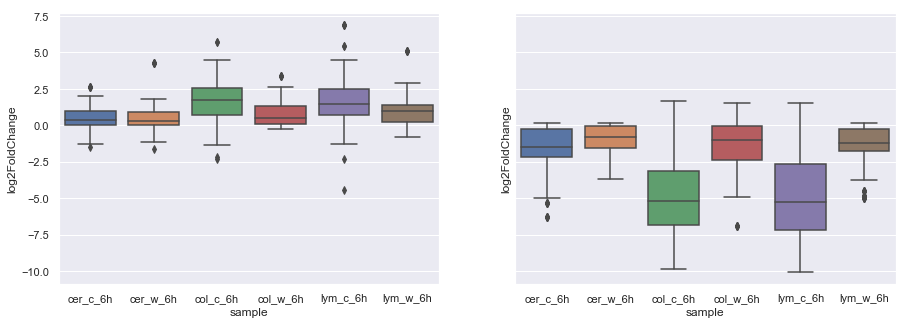
\includegraphics[width=.9\linewidth]{obipy-resources/pairings_timingsr_boxplots.png}
\caption{\label{pairings_timings_boxplots}
Boxplots of differential expressions from 50 largest (left) and 50 lowest (right) DE genes}
\end{figure}

\subsection{Lineplots of changes between samples for genes of interest}
\label{sec:org75ff674}

These lineplots are looking at the rate of change between the each sample's most up/down regulated genes (top 5 for each genotype/sample).\\

\begin{minted}[frame=lines,linenos=true,fontfamily=Monaco]{ipython}
import matplotlib.pyplot as plt
import seaborn as sns
import numpy as np
#DE_cross_time_pairings = read_xl('/Users/hughesn/PHD/Transcripts/Data/cross_time_pairings.xlsx')

def get_linedata(time_pair_df, n=5, include_large=True, include_small=True):
    top = time_pair_df.groupby(
        ['sample', 'gene']).mean().reset_index().set_index('gene')
    locs = get_locs(top, n, include_large=include_large,
                    include_small=include_small)
    tc = counts.loc[locs]
    tc = tc.T.reset_index()
    tc['sample'] = tc['index'].apply(lambda x: str(x).rsplit('_', 1)[0])
    tc = tc.set_index('index')
    tc = tc.reset_index().melt(id_vars=['index', 'sample'])
    tc.rename(columns={'index': 'id'}, inplace=True)
    tc['time'] = tc['sample'].apply(lambda x: str(x).rsplit('_', 1)[-1])
    tc['treatment'] = tc['id'].apply(lambda x: str(x).split('_')[1])
    tc['geno'] = tc['id'].apply(lambda x: str(x).split('_')[0])
    tc['sample'] = tc['sample'].apply(lambda x: str(x)[:5])
    return tc


def generate_plots_method_2(df):
    for s in df['sample'].unique():
        tdf = get_linedata(df[df['sample'] == s], include_small=False, include_large=True)
        fig, axes = plt.subplots(
            2, len(tdf['variable'].unique()), figsize=(20,8), sharex=True)
        j = -1
        for v in tdf['variable'].unique():
            i = 1
            j = j+1

            sns.lineplot(data=tdf[tdf['variable']==v], x='time', y='value', err_style="bars",
                         hue='geno', style="treatment", ax=axes[i, j], legend=False)
            axes[i, j].set_title(v)

        tdf = get_linedata(df[df['sample'] == s], include_small=True, include_large=False)
        j = -1
        for  v in tdf['variable'].unique():
            i = 0
            j = j+1
            if j+1 == len(tdf['variable'].unique()):
                sns.lineplot(data=tdf[tdf['variable']==v], x='time', y='value', err_style="bars",
                             hue='geno', style="treatment", ax=axes[i, j])
            else:
                sns.lineplot(data=tdf[tdf['variable']==v], x='time', y='value', err_style="bars",
                             hue='geno', style="treatment", ax=axes[i, j], legend=False)
            axes[i, j].set_title(v)

        fig.suptitle("Largest upreg (top row) and downreg (bottom row) DE genes for sample {0}".format(s))
        #fig.tight_layout()

sns.set(font_scale=1.3)
generate_plots_method_2(DE_cross_time_pairings)
\end{minted}

\begin{verbatim}
<Figure size 1440x576 with 10 Axes>
\end{verbatim}


\begin{center}
\includegraphics[width=.9\linewidth]{obipy-resources/e77a762dc857123716befe90c8377aaf6f2b9180/f3d5a18cd7a9db2b7932d2c39d9cb2a157dcbddb.png}
\end{center}

\begin{verbatim}
<Figure size 1440x576 with 10 Axes>
\end{verbatim}


\begin{center}
\includegraphics[width=.9\linewidth]{obipy-resources/e77a762dc857123716befe90c8377aaf6f2b9180/a18a7dcd50de4bf2616babb201fe1910ac575913.png}
\end{center}

\begin{verbatim}
<Figure size 1440x576 with 10 Axes>
\end{verbatim}


\begin{center}
\includegraphics[width=.9\linewidth]{obipy-resources/e77a762dc857123716befe90c8377aaf6f2b9180/12cb10060faa37a051e996d467773c67688b33ab.png}
\end{center}

\begin{verbatim}
<Figure size 1440x576 with 10 Axes>
\end{verbatim}


\begin{center}
\includegraphics[width=.9\linewidth]{obipy-resources/e77a762dc857123716befe90c8377aaf6f2b9180/f744a16dff67b1ad2df3ffc6d594647fad8f2083.png}
\end{center}

\begin{verbatim}
<Figure size 1440x576 with 10 Axes>
\end{verbatim}


\begin{center}
\includegraphics[width=.9\linewidth]{obipy-resources/e77a762dc857123716befe90c8377aaf6f2b9180/c759b1f22df033fa63fb7f0bb9fea987a40465a9.png}
\end{center}

\begin{verbatim}
<Figure size 1440x576 with 10 Axes>
\end{verbatim}


\begin{center}
\includegraphics[width=.9\linewidth]{obipy-resources/e77a762dc857123716befe90c8377aaf6f2b9180/96db5f9c761aa33f69a092661fd28188299ca931.png}
\end{center}


\subsection{Checking up and down data's largest}
\label{sec:org2bad081}

\begin{minted}[frame=lines,linenos=true,fontfamily=Monaco]{ipython}
DE_cross_time_pairings = read_xl('/Users/hughesn/PHD/Transcripts/Data/cross_time_pairings.xlsx')
n = 5
df = DE_cross_time_pairings
s = list(df['sample'].unique())[0]
#tdf =  get_linedata(df[df['sample'] == s], include_small=True, include_large=False)
#tdf.head(10)

df = df[df['sample'] == s]
top = df.groupby(
    ['sample', 'gene']).mean().reset_index().set_index('gene')
locs = get_locs(top, n, include_large=True,
                include_small=False)
top=top.loc[locs]
bot = df.groupby(
    ['sample', 'gene']).mean().reset_index().set_index('gene')
locs = get_locs(bot, n, include_large=False,
                include_small=True)
bot=bot.loc[locs]
top_and_bot = pd.concat([top, bot])
filter_cols = [c for c in counts if (c.startswith(s) or c.startswith(s.replace('05h', '6h')))]
pd.merge(top_and_bot, counts[filter_cols], left_index=True, right_index=True)

\end{minted}

\begin{center}
\begin{tabular}{llrrrrrrrrrrr}
 & sample & baseMean & log2FoldChange & lfcSE & pvalue & padj & lym\_c\_05h\_a21 & lym\_c\_05h\_b22 & lym\_c\_05h\_c23 & lym\_c\_6h\_a69 & lym\_c\_6h\_b70 & lym\_c\_6h\_d72\\
\hline
AT4G31950 & lym\_c\_05h & 62.134 & 10.0663 & 1.1773 & 1.21003e-20 & 3.04446e-19 & 9.02695 & 8.85273 & 8.77664 & 5.60783 & 5.60783 & 5.60783\\
AT1G05767 & lym\_c\_05h & 39.595 & 9.44474 & 1.19215 & 2.80169e-18 & 6.36071e-17 & 8.51408 & 8.23432 & 8.45238 & 5.60783 & 5.60783 & 5.60783\\
AT5G11140 & lym\_c\_05h & 193.93 & 9.1037 & 0.658458 & 3.39885e-46 & 1.77167e-44 & 10.0746 & 10.0683 & 10.2896 & 5.94226 & 5.60783 & 5.91306\\
AT3G02840 & lym\_c\_05h & 498.838 & 9.05894 & 0.723606 & 1.11048e-38 & 4.82548e-37 & 11.4503 & 11.3644 & 11.5624 & 5.60783 & 5.86799 & 6.28538\\
AT1G56242 & lym\_c\_05h & 578.043 & 8.64022 & 0.636589 & 1.40178e-44 & 7.0999e-43 & 12.0019 & 11.7486 & 11.9635 & 6.21527 & 6.09291 & 6.21495\\
AT4G31970 & lym\_c\_05h & 107.475 & -6.88759 & 1.58634 & 5.32543e-08 & 6.00415e-07 & 5.84268 & 5.60783 & 5.83302 & 9.51599 & 8.13272 & 7.91314\\
AT1G31173 & lym\_c\_05h & 29.224 & -6.87794 & 1.21362 & 7.69248e-11 & 1.12916e-09 & 5.60783 & 5.60783 & 5.60783 & 7.04642 & 6.68769 & 7.24795\\
AT3G60140 & lym\_c\_05h & 34.3907 & -5.44865 & 1.07682 & 8.40611e-09 & 1.03509e-07 & 5.93959 & 5.94093 & 5.60783 & 7.63482 & 7.20347 & 8.33776\\
AT1G49205 & lym\_c\_05h & 37.8818 & -4.46302 & 0.646491 & 3.5835e-13 & 6.1802e-12 & 5.84268 & 5.60783 & 6.10935 & 6.98954 & 7.20347 & 7.17624\\
AT4G37990 & lym\_c\_05h & 34.5777 & -4.26807 & 1.03037 & 1.34285e-06 & 1.26905e-05 & 5.60783 & 5.60783 & 6.15667 & 7.31197 & 6.86976 & 7.54442\\
\end{tabular}
\end{center}
\section{Selecting genes for Col0 at 05hr C/W}
\label{sec:org2db8c38}
\subsection{RFE selecting 25 genes}
\label{sec:org96a0218}
\begin{minted}[frame=lines,linenos=true,fontfamily=Monaco]{ipython}
from sklearn.feature_selection import RFE, RFECV
from sklearn.linear_model import LogisticRegression

# load data
DE_pairings_05hr = read_xl('/Users/hughesn/PHD/Transcripts/Data/pairings_05hr.xlsx')
sig = DE_pairings_05hr[DE_pairings_05hr['padj'] < 0.05]
sig = sig['log2FoldChange'].sort_values()
locs = sig.index
df = counts.loc[locs][[c for c in counts.columns if ('_05h' in c and 'col' in c)]].T
df = df.loc[:,~df.columns.duplicated()]
df = df[[c for c in set(df.columns.values)]]
\end{minted}

\begin{minted}[frame=lines,linenos=true,fontfamily=Monaco]{ipython}
# Feature Extraction with RFE
X = df.values
y = [y.rsplit('_',1)[0] for y in df.reset_index()['index']]
# feature extraction
model = LogisticRegression()
rfe = RFE(model, n_features_to_select=25)
fit = rfe.fit(X, y)
print("Num Features: {0}".format(fit.n_features_))
print("Selected Features: {0}".format(fit.support_))
print("Feature Ranking: {0}".format(fit.ranking_))
\end{minted}

Num Features: 25\\
Selected Features: [False False False \ldots{} False False False]\\
Feature Ranking: [1128  570 2984 \ldots{}   84  210 4723]\\


\begin{minted}[frame=lines,linenos=true,fontfamily=Monaco]{ipython}
genes = []
for r,f in zip(fit.ranking_, df.columns.values):
      if r ==1:
            genes.append(f)
get_gene_names(genes)
\end{minted}

\begin{center}
\begin{tabular}{rlll}
 & incoming & name & description\\
\hline
0 & AT5G60390 & A1 & Elongation factor 1-alpha 4\\
1 & AT3G59940 & SKIP20 & F-box/kelch-repeat protein SKIP20\\
2 & AT1G14540 & PER4 & Peroxidase\\
3 & AT5G59780 & MYB59 & Transcription factor MYB59\\
4 & AT5G61590 & ERF107 & Ethylene-responsive transcription factor ERF107\\
5 & AT1G68520 & COL6 & Zinc finger protein CONSTANS-LIKE 6\\
6 & AT2G37430 & ZAT11 & ZAT11\\
7 & AT5G27420 & ATL31 & E3 ubiquitin-protein ligase ATL31\\
8 & AT5G24110 & WRKY30 & Probable WRKY transcription factor 30\\
9 & AT3G02840 & AT3G02840 & ARM repeat superfamily protein\\
10 & AT1G66090 & AT1G66090 & Disease resistance protein (TIR-NBS class)\\
11 & AT3G09275 & AT3G09275 & None\\
12 & AT4G19700 & BOI & E3 ubiquitin-protein ligase BOI\\
13 & AT1G25440 & COL16 & Zinc finger protein CONSTANS-LIKE 16\\
14 & AT5G47230 & ERF5 & ERF5\\
15 & AT1G72520 & LOX4 & Lipoxygenase 4, chloroplastic\\
16 & AT1G56242 & AT1G56242 & other RNA\\
17 & AT5G11140 & AT5G11140 & Phospholipase-like protein (PEARLI 4) family protein\\
18 & AT5G37260 & RVE2 & Protein REVEILLE 2\\
19 & AT2G21210 & AT2G21210 & SAUR-like auxin-responsive protein family\\
20 & AT2G18440 & GUT15 & GUT15 (GENE WITH UNSTABLE TRANSCRIPT 15)\\
21 & AT1G56240 & PP2B13 & F-box protein PP2-B13\\
22 & AT1G07160 & AT1G07160 & PP2C-type phosphatase AP2C2\\
23 & AT4G38840 & AT4G38840 & At4g38840\\
24 & AT5G25350 & EBF2 & EIN3-binding F-box protein 2\\
\end{tabular}
\end{center}


\subsubsection{Forest on this RFE set}
\label{sec:org0c5f01c}

\begin{minted}[frame=lines,linenos=true,fontfamily=Monaco]{ipython}
rfe_forest = counts.loc[genes][[c for c in counts.columns if ('_05h' in c and 'col' in c)]].T
rfe_forest = rfe_forest.loc[:,~rfe_forest.columns.duplicated()]
rfe_forest = rfe_forest[[c for c in set(rfe_forest.columns.values)]]

feat_labels = rfe_forest.columns.values
y = [d.rsplit('_', 1)[0] for d in rfe_forest.index.values]

X_train, X_test, y_train, y_test = train_test_split(rfe_forest.values, y, test_size=1, random_state=42)
forest = RandomForestClassifier(n_estimators=20000, random_state=1, n_jobs=-1)
forest.fit(X_train, y_train)
res = {k: v for k, v in sorted(
    zip(feat_labels, forest.feature_importances_), key=lambda x: x[1], reverse=True)}
res_df = pd.DataFrame(list(res.items()), columns=[
                      'gene', 'importance']).set_index('gene')
names = get_gene_names(list(res_df.index))
res_df = pd.merge(res_df, names, left_index=True, right_on='incoming').rename(
    columns={'incoming': 'gene'}).set_index('gene').sort_values('importance', ascending=False)
res_df
\end{minted}

\begin{center}
\begin{tabular}{lrll}
gene & importance & name & description\\
\hline
AT2G21210 & 0.0405 & AT2G21210 & SAUR-like auxin-responsive protein family\\
AT1G56242 & 0.03945 & AT1G56242 & other RNA\\
AT5G47230 & 0.03905 & ERF5 & ERF5\\
AT3G59940 & 0.0385 & SKIP20 & F-box/kelch-repeat protein SKIP20\\
AT1G25440 & 0.0382 & COL16 & Zinc finger protein CONSTANS-LIKE 16\\
AT5G59780 & 0.03815 & MYB59 & Transcription factor MYB59\\
AT3G09275 & 0.0378 & AT3G09275 & None\\
AT4G38840 & 0.03765 & AT4G38840 & At4g38840\\
AT4G19700 & 0.0376 & BOI & E3 ubiquitin-protein ligase BOI\\
AT5G11140 & 0.03745 & AT5G11140 & Phospholipase-like protein (PEARLI 4) family protein\\
AT1G72520 & 0.03745 & LOX4 & Lipoxygenase 4, chloroplastic\\
AT1G66090 & 0.0372 & AT1G66090 & Disease resistance protein (TIR-NBS class)\\
AT3G02840 & 0.037 & AT3G02840 & ARM repeat superfamily protein\\
AT2G18440 & 0.03695 & GUT15 & GUT15 (GENE WITH UNSTABLE TRANSCRIPT 15)\\
AT5G27420 & 0.0369 & ATL31 & E3 ubiquitin-protein ligase ATL31\\
AT1G07160 & 0.0369 & AT1G07160 & PP2C-type phosphatase AP2C2\\
AT5G37260 & 0.03675 & RVE2 & Protein REVEILLE 2\\
AT2G37430 & 0.0366 & ZAT11 & ZAT11\\
AT5G25350 & 0.0362 & EBF2 & EIN3-binding F-box protein 2\\
AT1G68520 & 0.03585 & COL6 & Zinc finger protein CONSTANS-LIKE 6\\
AT5G61590 & 0.03585 & ERF107 & Ethylene-responsive transcription factor ERF107\\
AT1G14540 & 0.03555 & PER4 & Peroxidase\\
AT1G56240 & 0.03485 & PP2B13 & F-box protein PP2-B13\\
AT5G24110 & 0.0345 & WRKY30 & Probable WRKY transcription factor 30\\
AT5G60390 & 0.02005 & A1 & Elongation factor 1-alpha 4\\
\end{tabular}
\end{center}

\begin{minted}[frame=lines,linenos=true,fontfamily=Monaco]{ipython}
fig, ax = plt.subplots(1, figsize=(20,20))
sns.barplot(data=res_df.reset_index(), y='description', x='importance', ax=ax)
plt.tight_layout()
\end{minted}

\begin{verbatim}
<Figure size 1440x1440 with 1 Axes>
\end{verbatim}


\begin{center}
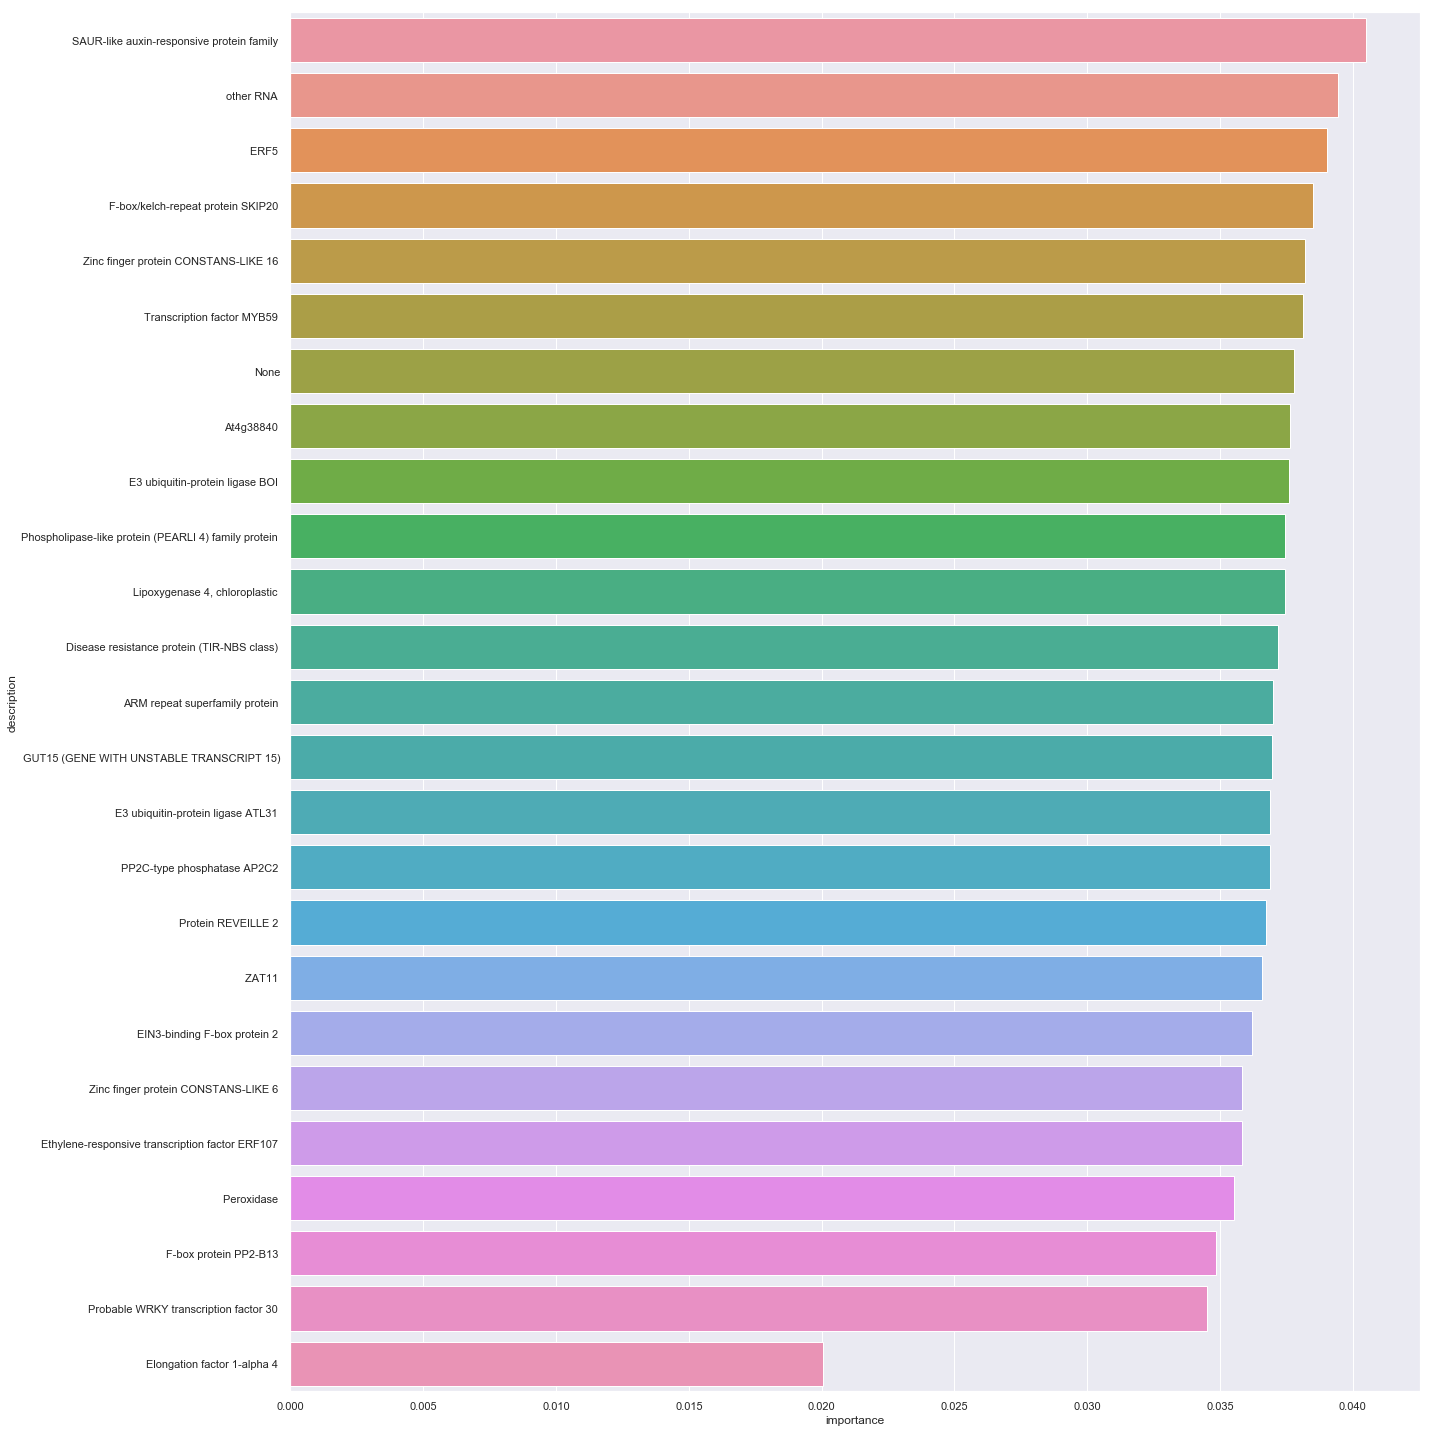
\includegraphics[width=.9\linewidth]{obipy-resources/93e2fbf76ed477962282ae99767b8408de4d3ed9/632b536b1900f336a7c3395fa110131ed5a5980a.png}
\end{center}


\subsection{RFE selecting 250 genes}
\label{sec:orgc3852db}
\begin{minted}[frame=lines,linenos=true,fontfamily=Monaco]{ipython}
from sklearn.feature_selection import RFE, RFECV
from sklearn.linear_model import LogisticRegression

# load data
DE_pairings_05hr = read_xl('/Users/hughesn/PHD/Transcripts/Data/pairings_05hr.xlsx')
sig = DE_pairings_05hr[DE_pairings_05hr['padj'] < 0.05]
sig = sig['log2FoldChange'].sort_values()
locs = sig.index
df = counts.loc[locs][[c for c in counts.columns if ('_05h' in c and 'col' in c)]].T
df = df.loc[:,~df.columns.duplicated()]
df = df[[c for c in set(df.columns.values)]]
\end{minted}

\begin{minted}[frame=lines,linenos=true,fontfamily=Monaco]{ipython}
# Feature Extraction with RFE
X = df.values
y = [y.rsplit('_',1)[0] for y in df.reset_index()['index']]
# feature extraction
model = LogisticRegression()
rfe = RFE(model, n_features_to_select=250)
fit = rfe.fit(X, y)
print("Num Features: {0}".format(fit.n_features_))
print("Selected Features: {0}".format(fit.support_))
print("Feature Ranking: {0}".format(fit.ranking_))
\end{minted}

Num Features: 250\\
Selected Features: [False False False \ldots{}  True  True False]\\
Feature Ranking: [ 903  345 2759 \ldots{}    1    1 4498]\\


\begin{minted}[frame=lines,linenos=true,fontfamily=Monaco]{ipython}
genes = []
for r,f in zip(fit.ranking_, df.columns.values):
      if r ==1:
            genes.append(f)
get_gene_names(genes)
\end{minted}



\begin{center}
\begin{tabular}{rlll}
 & incoming & name & description\\
\hline
0 & AT5G59820 & ZAT12 & Zinc finger protein ZAT12\\
1 & AT5G44130 & FLA13 & Fasciclin-like arabinogalactan protein 13\\
2 & AT1G79110 & BRG2 & Probable BOI-related E3 ubiquitin-protein ligase 2\\
3 & AT4G15975 & AT4G15975 & RING/U-box superfamily protein\\
4 & AT5G57760 & AT5G57760 & At5g57760\\
5 & AT4G14365 & XBAT34 & Putative E3 ubiquitin-protein ligase XBAT34\\
6 & AT1G78100 & AT1G78100 & AUF1\\
7 & AT1G78080 & RAP2-4 & Ethylene-responsive transcription factor RAP2-4\\
8 & AT3G16420 & PBP1 & PYK10-binding protein 1\\
9 & AT3G58120 & BZIP61 & BZIP61\\
10 & AT3G22121 & AT3G22121 & other RNA\\
11 & AT2G10940 & AT2G10940 & At2g10940/F15K19.1\\
12 & AT1G74470 & CHLP & Geranylgeranyl diphosphate reductase, chloroplastic\\
13 & AT3G04400 & RPL23A & 60S ribosomal protein L23\\
14 & AT5G25250 & FLOT1 & Flotillin-like protein 1\\
15 & AT5G60390 & A1 & Elongation factor 1-alpha 4\\
16 & AT5G01540 & LECRK62 & L-type lectin-domain containing receptor kinase VI.2\\
17 & AT5G49910 & HSP70-7 & Heat shock 70 kDa protein 7, chloroplastic\\
18 & AT4G14450 & AT4G14450 & Uncharacterized protein At4g14450, chloroplastic\\
19 & AT5G15870 & AT5G15870 & Glycosyl hydrolase family 81 protein\\
20 & AT5G61570 & AT5G61570 & Protein kinase superfamily protein\\
21 & AT3G09260 & BGLU23 & PYK10\\
22 & AT1G80840 & WRKY40 & Probable WRKY transcription factor 40\\
23 & AT5G57220 & CYP81F2 & Cytochrome P450 81F2\\
24 & AT2G25735 & AT2G25735 & Expressed protein\\
25 & AT5G51190 & ERF105 & Ethylene-responsive transcription factor ERF105\\
26 & AT5G41750 & AT5G41750 & Disease resistance protein (TIR-NBS-LRR class) family\\
27 & AT2G27660 & AT2G27660 & Cysteine/Histidine-rich C1 domain family protein\\
28 & AT5G56030 & HSP81-2 & Heat shock protein 81-2\\
29 & AT1G72910 & AT1G72910 & Similar to part of disease resistance protein\\
30 & AT3G59940 & SKIP20 & F-box/kelch-repeat protein SKIP20\\
31 & AT4G24570 & PUMP4 & DIC2\\
32 & AT1G79680 & WAKL10 & Wall-associated receptor kinase-like 10\\
33 & AT3G04840 & RPS3AA & 40S ribosomal protein S3a-1\\
34 & AT4G16370 & ATOPT3 & oligopeptide transporter\\
35 & AT2G35935 & AT2G35935 & None\\
36 & AT5G64905 & PEP3 & Elicitor peptide 3\\
37 & AT1G17147 & VQ1 & VQ motif-containing protein 1\\
38 & AT5G25340 & AT5G25340 & Ubiquitin-like superfamily protein\\
39 & AT4G34760 & SAUR50 & Auxin-responsive protein SAUR50\\
40 & AT1G24140 & 3MMP & Metalloendoproteinase 3-MMP\\
41 & AT1G14540 & PER4 & Peroxidase\\
42 & AT3G23250 & MYB15 & Transcription factor MYB15\\
43 & AT2G36530 & ENO2 & LOS2\\
44 & AT4G23810 & WRKY53 & Probable WRKY transcription factor 53\\
45 & AT2G01180 & ATPAP1 & phosphatidic acid phosphatase 1\\
46 & AT5G59780 & MYB59 & Transcription factor MYB59\\
47 & AT2G45180 & AT2G45180 & At2g45180/T14P1.1\\
48 & AT3G07195 & AT3G07195 & RPM1-interacting protein 4 (RIN4) family protein\\
49 & AT1G48300 & AT1G48300 & unknown protein\\
50 & AT5G28610 & AT5G28610 & LOW protein: ATP-dependent RNA helicase DRS1-like protein\\
51 & AT3G63200 & PLP9 & Probable inactive patatin-like protein 9\\
52 & AT1G07135 & AT1G07135 & At1g07135\\
53 & AT1G09780 & PGM1 & IPGAM1\\
54 & AT3G25520 & ATL5 & RPL5A\\
55 & AT4G38860 & AT4G38860 & At4g38860\\
56 & AT1G12090 & ELP & ELP\\
57 & AT4G29780 & AT4G29780 & Nuclease\\
58 & AT3G49010 & RPL13B & 60S ribosomal protein L13-1\\
59 & AT4G02410 & LECRK43 & L-type lectin-domain containing receptor kinase IV.3\\
60 & AT2G36690 & AT2G36690 & 2-oxoglutarate (2OG) and Fe(II)-dependent oxygenase superfamily protein\\
61 & AT4G14370 & AT4G14370 & Disease resistance protein (TIR-NBS-LRR class) family\\
62 & AT4G38620 & MYB4 & Transcription repressor MYB4\\
63 & AT5G61590 & ERF107 & Ethylene-responsive transcription factor ERF107\\
64 & AT2G41840 & RPS2C & 40S ribosomal protein S2-3\\
65 & AT2G44670 & FLZ3 & FCS-Like Zinc finger 3\\
66 & AT1G05675 & UGT74E1 & Glycosyltransferase (Fragment)\\
67 & AT1G65390 & PP2A5 & Protein PHLOEM PROTEIN 2-LIKE A5\\
68 & AT4G34950 & AT4G34950 & Major facilitator superfamily protein\\
69 & AT5G02500 & MED37E & Probable mediator of RNA polymerase II transcription subunit 37e\\
70 & AT1G68520 & COL6 & Zinc finger protein CONSTANS-LIKE 6\\
71 & AT1G56250 & VBF & F-box protein VBF\\
72 & AT4G18197 & PUP7 & Probable purine permease 7\\
73 & AT5G52050 & DTX50 & Protein DETOXIFICATION 50\\
74 & AT5G20290 & RPS8A & 40S ribosomal protein S8\\
75 & AT1G27730 & ZAT10 & Zinc finger protein ZAT10\\
76 & AT4G13930 & SHM4 & Serine hydroxymethyltransferase 4\\
77 & AT3G44260 & CAF1-9 & Probable CCR4-associated factor 1 homolog 9\\
78 & AT2G37430 & ZAT11 & ZAT11\\
79 & AT5G02870 & RPL4D & 60S ribosomal protein L4-2\\
80 & AT3G09630 & RPL4A & 60S ribosomal protein L4-1\\
81 & AT5G03240 & UBQ3 & Ubiquitin 4\\
82 & AT5G65310 & ATHB-5 & Homeobox-leucine zipper protein ATHB-5\\
83 & AT5G27420 & ATL31 & E3 ubiquitin-protein ligase ATL31\\
84 & AT4G27280 & KRP1 & Calcium-binding protein KRP1\\
85 & AT3G29000 & CML45 & Probable calcium-binding protein CML45\\
86 & AT5G24110 & WRKY30 & Probable WRKY transcription factor 30\\
87 & AT5G61600 & ERF104 & Ethylene-responsive transcription factor ERF104\\
88 & AT5G15845 & AT5G15845 & other RNA\\
89 & AT4G16720 & RPL15A & Ribosomal protein L15\\
90 & AT3G02840 & AT3G02840 & ARM repeat superfamily protein\\
91 & AT5G17920 & MS1 & 5-methyltetrahydropteroyltriglutamate--homocysteine methyltransferase 1\\
92 & AT3G53870 & RPS3B & 40S ribosomal protein S3-2\\
93 & AT1G66090 & AT1G66090 & Disease resistance protein (TIR-NBS class)\\
94 & AT1G67430 & RPL17B & 60S ribosomal protein L17-2\\
95 & AT5G19240 & AT5G19240 & Uncharacterized GPI-anchored protein At5g19240\\
96 & AT3G09275 & AT3G09275 & None\\
97 & AT3G18710 & PUB29 & RING-type E3 ubiquitin transferase\\
98 & AT4G37540 & LBD39 & LOB domain-containing protein 39\\
99 & AT2G02950 & PKS1 & Protein PHYTOCHROME KINASE SUBSTRATE 1\\
100 & AT2G26560 & PLP2 & Patatin-like protein 2\\
101 & AT1G50040 & AT1G50040 & F2J10.8 protein\\
102 & AT1G18540 & RPL6A & 60S ribosomal protein L6-1\\
103 & AT3G05590 & RPL18B & RPL18\\
104 & AT3G62870 & RPL7AB & 60S ribosomal protein L7a-2\\
105 & AT4G01250 & WRKY22 & WRKY transcription factor 22\\
106 & AT2G27820 & ADT3 & Arogenate dehydratase 3, chloroplastic\\
107 & AT1G05575 & AT1G05575 & Transmembrane protein\\
108 & AT1G61360 & AT1G61360 & Serine/threonine-protein kinase\\
109 & AT5G18380 & RPS16C & 40S ribosomal protein S16-3\\
110 & AT1G30370 & AT1G30370 & DLAH\\
111 & AT3G09500 & RPL35A & 60S ribosomal protein L35-1\\
112 & AT2G40000 & HSPRO2 & Nematode resistance protein-like HSPRO2\\
113 & AT1G78170 & AT1G78170 & E3 ubiquitin-protein ligase\\
114 & AT1G59590 & ZCF37 & At1g59590\\
115 & AT4G19700 & BOI & E3 ubiquitin-protein ligase BOI\\
116 & AT5G05300 & AT5G05300 & Gb\\
117 & AT3G53460 & CP29 & Chloroplast RNA-binding protein 29\\
118 & AT1G18080 & RACK1A & RACK1A\_AT\\
119 & AT2G22880 & AT2G22880 & At2g22880\\
120 & AT5G26742 & RH3 & RH3\\
121 & AT2G08475 & AT2G08475 & None\\
122 & AT4G22030 & AT4G22030 & F-box family protein with a domain of unknown function (DUF295)\\
123 & AT1G25440 & COL16 & Zinc finger protein CONSTANS-LIKE 16\\
124 & AT2G32030 & AT2G32030 & Acyl-CoA N-acyltransferases (NAT) superfamily protein\\
125 & AT3G09200 & RPP0B & 60S acidic ribosomal protein P0-2\\
126 & AT1G68550 & ERF118 & Ethylene-responsive transcription factor ERF118\\
127 & AT4G22710 & CYP706A2 & Cytochrome P450 - like protein\\
128 & AT3G22120 & CWLP & Cell wall-plasma membrane linker protein\\
129 & AT3G21150 & BBX32 & B-box zinc finger protein 32\\
130 & AT5G56010 & HSP90-3 & Heat shock protein 90-3\\
131 & AT1G57990 & PUP18 & PUP18\\
132 & AT1G80080 & TMM & TMM\\
133 & AT2G02630 & AT2G02630 & Cysteine/Histidine-rich C1 domain family protein\\
134 & AT4G23220 & CRK14 & Cysteine-rich receptor-like protein kinase 14\\
135 & AT1G26380 & FOX1 & Berberine bridge enzyme-like 3\\
136 & AT3G46130 & ATMYB48 & myb domain protein 48\\
137 & AT5G47230 & ERF5 & ERF5\\
138 & AT1G13930 & AT1G13930 & At1g13930/F16A14.27\\
139 & AT1G24145 & AT1G24145 & At1g24145\\
140 & AT1G50750 & AT1G50750 & Plant mobile domain protein family\\
141 & AT5G25280 & AT5G25280 & AT5g25280/F18G18\_20\\
142 & AT5G47850 & CCR4 & Serine/threonine-protein kinase-like protein CCR4\\
143 & AT1G72520 & LOX4 & Lipoxygenase 4, chloroplastic\\
144 & AT5G41740 & AT5G41740 & Disease resistance protein (TIR-NBS-LRR class) family\\
145 & AT5G44680 & AT5G44680 & DNA glycosylase superfamily protein\\
146 & AT3G03125 & AT3G03125 & None\\
147 & AT1G19020 & AT1G19020 & CDP-diacylglycerol-glycerol-3-phosphate 3-phosphatidyltransferase\\
148 & AT5G52750 & HIPP13 & Heavy metal-associated isoprenylated plant protein 13\\
149 & AT5G20230 & BCB & SAG14\\
150 & AT1G56242 & AT1G56242 & other RNA\\
151 & AT2G31345 & AT2G31345 & Transmembrane protein\\
152 & AT1G10020 & AT1G10020 & At1g10020\\
153 & AT4G11470 & CRK31 & cysteine-rich RLK (RECEPTOR-like protein kinase) 31\\
154 & AT2G38310 & PYL4 & Abscisic acid receptor PYL4\\
155 & AT5G22250 & CAF1-11 & Probable CCR4-associated factor 1 homolog 11\\
156 & AT5G14700 & AT5G14700 & Cinnamoyl CoA reductase-like protein\\
157 & AT1G61340 & AT1G61340 & F-box protein At1g61340\\
158 & AT1G69530 & ATEXPA1 & Expansin\\
159 & AT4G37370 & CYP81D8 & Cytochrome P450, family 81, subfamily D, polypeptide 8\\
160 & AT2G18020 & RPL8A & EMB2296\\
161 & AT2G34480 & AT2G34480 & Ribosomal protein L18ae/LX family protein\\
162 & AT1G20310 & AT1G20310 & Syringolide-induced protein\\
163 & AT5G11140 & AT5G11140 & Phospholipase-like protein (PEARLI 4) family protein\\
164 & AT2G18160 & BZIP2 & bZIP transcription factor 2\\
165 & AT1G72370 & RPSAA & 40S ribosomal protein SA\\
166 & AT5G20630 & GER3 & Germin-like protein subfamily 3 member 3\\
167 & AT3G19680 & AT3G19680 & Uncharacterized protein At3g19680\\
168 & AT3G22970 & AT3G22970 & At3g22970\\
169 & AT5G37260 & RVE2 & Protein REVEILLE 2\\
170 & AT5G04340 & ZAT6 & Zinc finger protein ZAT6\\
171 & AT5G67480 & BT4 & BTB and TAZ domain protein 4\\
172 & AT2G44840 & ERF13 & Ethylene-responsive transcription factor 13\\
173 & AT4G36648 & AT4G36648 & other RNA\\
174 & AT4G17390 & RPL15B & 60S ribosomal protein L15-2\\
175 & AT2G21210 & AT2G21210 & SAUR-like auxin-responsive protein family\\
176 & AT1G73540 & NUDT21 & Nudix hydrolase 21, chloroplastic\\
177 & AT3G01165 & AT3G01165 & None\\
178 & AT3G28340 & GATL10 & Hexosyltransferase (Fragment)\\
179 & AT2G36090 & AT2G36090 & Probable F-box protein At2g36090\\
180 & AT1G61560 & MLO6 & MLO-like protein 6\\
181 & AT2G30520 & RPT2 & Root phototropism protein 2\\
182 & AT1G58420 & AT1G58420 & At1g58420\\
183 & AT3G53430 & RPL12B & 60S ribosomal Protein L12-like\\
184 & AT1G17420 & LOX3 & Lipoxygenase 3, chloroplastic\\
185 & AT1G12820 & AFB3 & Protein AUXIN SIGNALING F-BOX 3\\
186 & AT1G56070 & LOS1 & Elongation factor 2\\
187 & AT2G21660 & RBG7 & Glycine-rich RNA-binding protein 7\\
188 & AT2G18440 & GUT15 & GUT15 (GENE WITH UNSTABLE TRANSCRIPT 15)\\
189 & AT5G15200 & RPS9B & 40S ribosomal protein S9-1\\
190 & AT3G50930 & HSR4 & Protein HYPER-SENSITIVITY-RELATED 4\\
191 & AT4G23180 & CRK10 & Cysteine-rich receptor-like protein kinase 10\\
192 & AT1G19770 & PUP14 & PUP14\\
193 & AT5G26920 & CBP60G & Calmodulin-binding protein 60 G\\
194 & AT5G02760 & AT5G02760 & Probable protein phosphatase 2C 67\\
195 & AT5G47210 & RGGC & RGG repeats nuclear RNA binding protein C\\
196 & AT2G40330 & PYL6 & Abscisic acid receptor PYL6\\
197 & AT1G70600 & RPL27AC & 60S ribosomal protein L27a-3\\
198 & AT2G28000 & CPN60A1 & SLP\\
199 & AT2G31880 & SOBIR1 & Leucine-rich repeat receptor-like serine/threonine/tyrosine-protein kinase SOBIR1\\
200 & AT4G18100 & RPL32A & 60S ribosomal protein L32-1\\
201 & AT4G31550 & WRKY11 & Probable WRKY transcription factor 11\\
202 & AT2G47440 & AT2G47440 & Tetratricopeptide repeat (TPR)-like superfamily protein\\
203 & AT2G23270 & AT2G23270 & At2g23270\\
204 & AT1G76600 & AT1G76600 & Poly polymerase\\
205 & AT2G29110 & ATGLR2.8 & Glutamate receptor\\
206 & AT1G14320 & RPL10A & 60S ribosomal protein L10-1\\
207 & AT1G09690 & RPL21A & 60S ribosomal protein L21-1\\
208 & AT5G59732 & AT5G59732 & other RNA\\
209 & AT1G56240 & PP2B13 & F-box protein PP2-B13\\
210 & AT5G13930 & CHS & Chalcone synthase family protein\\
211 & AT4G31950 & CYP82C3 & CYP82C3\\
212 & AT4G36500 & AT4G36500 & Uncharacterized protein At4g36500\\
213 & AT2G33580 & LYK5 & Protein LYK5\\
214 & AT5G65630 & GTE7 & Transcription factor GTE7\\
215 & AT1G07160 & AT1G07160 & PP2C-type phosphatase AP2C2\\
216 & AT2G38470 & WRKY33 & WRKY33\\
217 & AT4G39260 & RBG8 & GRP8\\
218 & AT4G17490 & ERF6 & Ethylene-responsive transcription factor 6\\
219 & AT2G40140 & CZF1 & Zinc finger CCCH domain-containing protein 29\\
220 & AT5G01542 & AT5G01542 & Potential natural antisense gene, locus overlaps with AT5G01540\\
221 & AT1G43170 & ARP1 & 60S ribosomal protein L3-1\\
222 & AT1G15690 & AVP1 & VHP1\\
223 & AT1G69890 & AT1G69890 & Actin cross-linking protein (DUF569)\\
224 & AT4G38840 & AT4G38840 & At4g38840\\
225 & AT2G17040 & anac036 & NAC domain containing protein 36\\
226 & AT3G10930 & AT3G10930 & Uncharacterized protein At3g10930\\
227 & AT5G25350 & EBF2 & EIN3-binding F-box protein 2\\
228 & AT3G62980 & TIR1 & TIR1\\
229 & AT1G21120 & AT1G21120 & O-methyltransferase family protein\\
230 & AT1G72600 & AT1G72600 & At1g72600\\
231 & AT1G69760 & AT1G69760 & At1g69760\\
232 & AT1G72610 & GLP1 & Germin-like protein subfamily 3 member 1\\
233 & AT4G13940 & SAHH1 & Adenosylhomocysteinase 1\\
234 & AT3G55980 & SZF1 & Salt-inducible zinc finger 1\\
235 & AT5G59730 & ATEXO70H7 & Exocyst subunit Exo70 family protein\\
236 & AT1G72430 & SAUR78 & Auxin-responsive protein SAUR78\\
237 & AT5G42380 & CML37 & Calcium-binding protein CML37\\
238 & AT1G21326 & AT1G21326 & F16F4.1 protein\\
239 & AT3G60245 & RPL37AC & 60S ribosomal protein L37a-2\\
240 & AT2G26530 & AR781 & AR781\\
241 & AT2G24600 & AT2G24600 & Ankyrin repeat family protein\\
242 & AT3G23810 & SAHH2 & Adenosylhomocysteinase\\
243 & AT2G43340 & AT2G43340 & At2g43340\\
244 & AT1G74850 & PTAC2 & PTAC2\\
245 & AT2G35930 & PUB23 & E3 ubiquitin-protein ligase PUB23\\
246 & AT2G23130 & AGP17 & Lysine-rich arabinogalactan protein 17\\
247 & AT4G28460 & PIP1 & PAMP-induced secreted peptide 1\\
248 & AT1G02780 & RPL19A & 60S ribosomal protein L19-1\\
249 & AT3G52400 & SYP122 & Syntaxin-122\\
\end{tabular}
\end{center}


\paragraph{Forest on this RFE set}
\label{sec:org9ddfa98}

\begin{minted}[frame=lines,linenos=true,fontfamily=Monaco]{ipython}
rfe_forest = counts.loc[genes][[c for c in counts.columns if ('_05h' in c and 'col' in c)]].T
rfe_forest = rfe_forest.loc[:,~rfe_forest.columns.duplicated()]
rfe_forest = rfe_forest[[c for c in set(rfe_forest.columns.values)]]

feat_labels = rfe_forest.columns.values
y = [d.rsplit('_', 1)[0] for d in rfe_forest.index.values]

X_train, X_test, y_train, y_test = train_test_split(rfe_forest.values, y, test_size=1, random_state=42)
forest = RandomForestClassifier(n_estimators=20000, random_state=1, n_jobs=-1)
forest.fit(X_train, y_train)
res = {k: v for k, v in sorted(
    zip(feat_labels, forest.feature_importances_), key=lambda x: x[1], reverse=True)}
res_df = pd.DataFrame(list(res.items()), columns=[
                      'gene', 'importance']).set_index('gene')
names = get_gene_names(list(res_df.index))
res_df = pd.merge(res_df, names, left_index=True, right_on='incoming').rename(
    columns={'incoming': 'gene'}).set_index('gene').sort_values('importance', ascending=False)
res_df
\end{minted}

\begin{center}
\begin{tabular}{lrll}
gene & importance & name & description\\
\hline
AT2G45180 & 0.0048 & AT2G45180 & At2g45180/T14P1.1\\
AT2G32030 & 0.00475 & AT2G32030 & Acyl-CoA N-acyltransferases (NAT) superfamily protein\\
AT1G72430 & 0.00465 & SAUR78 & Auxin-responsive protein SAUR78\\
AT1G56240 & 0.00465 & PP2B13 & F-box protein PP2-B13\\
AT2G27820 & 0.00455 & ADT3 & Arogenate dehydratase 3, chloroplastic\\
AT2G40330 & 0.0045 & PYL6 & Abscisic acid receptor PYL6\\
AT5G51190 & 0.0045 & ERF105 & Ethylene-responsive transcription factor ERF105\\
AT1G12090 & 0.00445 & ELP & ELP\\
AT4G23220 & 0.00445 & CRK14 & Cysteine-rich receptor-like protein kinase 14\\
AT5G26920 & 0.00445 & CBP60G & Calmodulin-binding protein 60 G\\
AT1G43170 & 0.00445 & ARP1 & 60S ribosomal protein L3-1\\
AT5G02870 & 0.0044 & RPL4D & 60S ribosomal protein L4-2\\
AT1G07135 & 0.00435 & AT1G07135 & At1g07135\\
AT3G23250 & 0.00435 & MYB15 & Transcription factor MYB15\\
AT2G38470 & 0.00435 & WRKY33 & WRKY33\\
AT4G18100 & 0.00435 & RPL32A & 60S ribosomal protein L32-1\\
AT1G24145 & 0.00435 & AT1G24145 & At1g24145\\
AT3G01165 & 0.0043 & AT3G01165 & None\\
AT5G15870 & 0.0043 & AT5G15870 & Glycosyl hydrolase family 81 protein\\
AT1G70600 & 0.0043 & RPL27AC & 60S ribosomal protein L27a-3\\
AT1G27730 & 0.0043 & ZAT10 & Zinc finger protein ZAT10\\
AT3G23810 & 0.0043 & SAHH2 & Adenosylhomocysteinase\\
AT5G59732 & 0.0043 & AT5G59732 & other RNA\\
AT4G18197 & 0.00425 & PUP7 & Probable purine permease 7\\
AT5G59780 & 0.00425 & MYB59 & Transcription factor MYB59\\
AT5G57220 & 0.00425 & CYP81F2 & Cytochrome P450 81F2\\
AT5G44130 & 0.00425 & FLA13 & Fasciclin-like arabinogalactan protein 13\\
AT5G03240 & 0.0042 & UBQ3 & Ubiquitin 4\\
AT2G44670 & 0.0042 & FLZ3 & FCS-Like Zinc finger 3\\
AT1G09780 & 0.0042 & PGM1 & IPGAM1\\
AT4G13930 & 0.0042 & SHM4 & Serine hydroxymethyltransferase 4\\
AT3G29000 & 0.0042 & CML45 & Probable calcium-binding protein CML45\\
AT1G68550 & 0.0042 & ERF118 & Ethylene-responsive transcription factor ERF118\\
AT1G72600 & 0.0042 & AT1G72600 & At1g72600\\
AT4G22030 & 0.0042 & AT4G22030 & F-box family protein with a domain of unknown function (DUF295)\\
AT4G23180 & 0.00415 & CRK10 & Cysteine-rich receptor-like protein kinase 10\\
AT4G16720 & 0.00415 & RPL15A & Ribosomal protein L15\\
AT2G28000 & 0.00415 & CPN60A1 & SLP\\
AT1G57990 & 0.00415 & PUP18 & PUP18\\
AT3G09500 & 0.00415 & RPL35A & 60S ribosomal protein L35-1\\
AT1G10020 & 0.00415 & AT1G10020 & At1g10020\\
AT2G25735 & 0.00415 & AT2G25735 & Expressed protein\\
AT2G44840 & 0.00415 & ERF13 & Ethylene-responsive transcription factor 13\\
AT3G22121 & 0.0041 & AT3G22121 & other RNA\\
AT2G17040 & 0.0041 & anac036 & NAC domain containing protein 36\\
AT5G22250 & 0.0041 & CAF1-11 & Probable CCR4-associated factor 1 homolog 11\\
AT4G36648 & 0.0041 & AT4G36648 & other RNA\\
AT1G56070 & 0.0041 & LOS1 & Elongation factor 2\\
AT3G04400 & 0.00405 & RPL23A & 60S ribosomal protein L23\\
AT1G58420 & 0.00405 & AT1G58420 & At1g58420\\
AT2G02950 & 0.00405 & PKS1 & Protein PHYTOCHROME KINASE SUBSTRATE 1\\
AT5G02500 & 0.00405 & MED37E & Probable mediator of RNA polymerase II transcription subunit 37e\\
AT2G40000 & 0.00405 & HSPRO2 & Nematode resistance protein-like HSPRO2\\
AT1G72610 & 0.00405 & GLP1 & Germin-like protein subfamily 3 member 1\\
AT1G14540 & 0.00405 & PER4 & Peroxidase\\
AT1G72910 & 0.004 & AT1G72910 & Similar to part of disease resistance protein\\
AT2G18440 & 0.004 & GUT15 & GUT15 (GENE WITH UNSTABLE TRANSCRIPT 15)\\
AT5G47210 & 0.004 & RGGC & RGG repeats nuclear RNA binding protein C\\
AT2G41840 & 0.004 & RPS2C & 40S ribosomal protein S2-3\\
AT5G57760 & 0.004 & AT5G57760 & At5g57760\\
AT3G09200 & 0.004 & RPP0B & 60S acidic ribosomal protein P0-2\\
AT1G50040 & 0.004 & AT1G50040 & F2J10.8 protein\\
AT5G20290 & 0.004 & RPS8A & 40S ribosomal protein S8\\
AT2G38310 & 0.004 & PYL4 & Abscisic acid receptor PYL4\\
AT4G22710 & 0.004 & CYP706A2 & Cytochrome P450 - like protein\\
AT3G22120 & 0.004 & CWLP & Cell wall-plasma membrane linker protein\\
AT1G69530 & 0.004 & ATEXPA1 & Expansin\\
AT2G18160 & 0.00395 & BZIP2 & bZIP transcription factor 2\\
AT5G59730 & 0.00395 & ATEXO70H7 & Exocyst subunit Exo70 family protein\\
AT4G34760 & 0.00395 & SAUR50 & Auxin-responsive protein SAUR50\\
AT2G36690 & 0.00395 & AT2G36690 & 2-oxoglutarate (2OG) and Fe(II)-dependent oxygenase superfamily protein\\
AT3G07195 & 0.00395 & AT3G07195 & RPM1-interacting protein 4 (RIN4) family protein\\
AT2G10940 & 0.00395 & AT2G10940 & At2g10940/F15K19.1\\
AT1G80840 & 0.0039 & WRKY40 & Probable WRKY transcription factor 40\\
AT4G31550 & 0.0039 & WRKY11 & Probable WRKY transcription factor 11\\
AT5G67480 & 0.0039 & BT4 & BTB and TAZ domain protein 4\\
AT1G48300 & 0.0039 & AT1G48300 & unknown protein\\
AT2G37430 & 0.0039 & ZAT11 & ZAT11\\
AT4G14365 & 0.0039 & XBAT34 & Putative E3 ubiquitin-protein ligase XBAT34\\
AT5G24110 & 0.0039 & WRKY30 & Probable WRKY transcription factor 30\\
AT2G43340 & 0.0039 & AT2G43340 & At2g43340\\
AT1G72370 & 0.0039 & RPSAA & 40S ribosomal protein SA\\
AT4G13940 & 0.00385 & SAHH1 & Adenosylhomocysteinase 1\\
AT2G47440 & 0.00385 & AT2G47440 & Tetratricopeptide repeat (TPR)-like superfamily protein\\
AT3G18710 & 0.00385 & PUB29 & RING-type E3 ubiquitin transferase\\
AT1G73540 & 0.00385 & NUDT21 & Nudix hydrolase 21, chloroplastic\\
AT1G80080 & 0.00385 & TMM & TMM\\
AT3G59940 & 0.00385 & SKIP20 & F-box/kelch-repeat protein SKIP20\\
AT5G14700 & 0.00385 & AT5G14700 & Cinnamoyl CoA reductase-like protein\\
AT2G31345 & 0.00385 & AT2G31345 & Transmembrane protein\\
AT2G36090 & 0.00385 & AT2G36090 & Probable F-box protein At2g36090\\
AT1G25440 & 0.00385 & COL16 & Zinc finger protein CONSTANS-LIKE 16\\
AT4G19700 & 0.00385 & BOI & E3 ubiquitin-protein ligase BOI\\
AT1G19020 & 0.00385 & AT1G19020 & CDP-diacylglycerol-glycerol-3-phosphate 3-phosphatidyltransferase\\
AT5G13930 & 0.00385 & CHS & Chalcone synthase family protein\\
AT5G61590 & 0.00385 & ERF107 & Ethylene-responsive transcription factor ERF107\\
AT5G19240 & 0.0038 & AT5G19240 & Uncharacterized GPI-anchored protein At5g19240\\
AT1G24140 & 0.0038 & 3MMP & Metalloendoproteinase 3-MMP\\
AT5G25280 & 0.0038 & AT5G25280 & AT5g25280/F18G18\_20\\
AT1G69760 & 0.0038 & AT1G69760 & At1g69760\\
AT5G56010 & 0.0038 & HSP90-3 & Heat shock protein 90-3\\
AT5G20630 & 0.0038 & GER3 & Germin-like protein subfamily 3 member 3\\
AT2G33580 & 0.0038 & LYK5 & Protein LYK5\\
AT2G29110 & 0.0038 & ATGLR2.8 & Glutamate receptor\\
AT2G26560 & 0.0038 & PLP2 & Patatin-like protein 2\\
AT5G52050 & 0.0038 & DTX50 & Protein DETOXIFICATION 50\\
AT4G27280 & 0.0038 & KRP1 & Calcium-binding protein KRP1\\
AT1G21120 & 0.0038 & AT1G21120 & O-methyltransferase family protein\\
AT1G74470 & 0.00375 & CHLP & Geranylgeranyl diphosphate reductase, chloroplastic\\
AT1G61360 & 0.00375 & AT1G61360 & Serine/threonine-protein kinase\\
AT5G27420 & 0.00375 & ATL31 & E3 ubiquitin-protein ligase ATL31\\
AT3G28340 & 0.00375 & GATL10 & Hexosyltransferase (Fragment)\\
AT1G50750 & 0.00375 & AT1G50750 & Plant mobile domain protein family\\
AT5G02760 & 0.00375 & AT5G02760 & Probable protein phosphatase 2C 67\\
AT2G36530 & 0.00375 & ENO2 & LOS2\\
AT3G52400 & 0.00375 & SYP122 & Syntaxin-122\\
AT4G14450 & 0.0037 & AT4G14450 & Uncharacterized protein At4g14450, chloroplastic\\
AT5G59820 & 0.0037 & ZAT12 & Zinc finger protein ZAT12\\
AT1G78170 & 0.0037 & AT1G78170 & E3 ubiquitin-protein ligase\\
AT1G68520 & 0.0037 & COL6 & Zinc finger protein CONSTANS-LIKE 6\\
AT1G26380 & 0.0037 & FOX1 & Berberine bridge enzyme-like 3\\
AT3G10930 & 0.0037 & AT3G10930 & Uncharacterized protein At3g10930\\
AT5G18380 & 0.0037 & RPS16C & 40S ribosomal protein S16-3\\
AT1G76600 & 0.0037 & AT1G76600 & Poly polymerase\\
AT2G24600 & 0.0037 & AT2G24600 & Ankyrin repeat family protein\\
AT3G50930 & 0.0037 & HSR4 & Protein HYPER-SENSITIVITY-RELATED 4\\
AT3G55980 & 0.0037 & SZF1 & Salt-inducible zinc finger 1\\
AT3G53870 & 0.0037 & RPS3B & 40S ribosomal protein S3-2\\
AT3G19680 & 0.00365 & AT3G19680 & Uncharacterized protein At3g19680\\
AT1G61560 & 0.00365 & MLO6 & MLO-like protein 6\\
AT3G05590 & 0.00365 & RPL18B & RPL18\\
AT4G38860 & 0.00365 & AT4G38860 & At4g38860\\
AT3G53430 & 0.00365 & RPL12B & 60S ribosomal Protein L12-like\\
AT1G05575 & 0.00365 & AT1G05575 & Transmembrane protein\\
AT4G14370 & 0.00365 & AT4G14370 & Disease resistance protein (TIR-NBS-LRR class) family\\
AT5G65630 & 0.00365 & GTE7 & Transcription factor GTE7\\
AT1G13930 & 0.00365 & AT1G13930 & At1g13930/F16A14.27\\
AT1G09690 & 0.00365 & RPL21A & 60S ribosomal protein L21-1\\
AT1G79110 & 0.00365 & BRG2 & Probable BOI-related E3 ubiquitin-protein ligase 2\\
AT1G02780 & 0.0036 & RPL19A & 60S ribosomal protein L19-1\\
AT2G01180 & 0.0036 & ATPAP1 & phosphatidic acid phosphatase 1\\
AT1G18540 & 0.0036 & RPL6A & 60S ribosomal protein L6-1\\
AT2G23130 & 0.0036 & AGP17 & Lysine-rich arabinogalactan protein 17\\
AT3G21150 & 0.0036 & BBX32 & B-box zinc finger protein 32\\
AT1G78080 & 0.0036 & RAP2-4 & Ethylene-responsive transcription factor RAP2-4\\
AT1G19770 & 0.0036 & PUP14 & PUP14\\
AT1G12820 & 0.0036 & AFB3 & Protein AUXIN SIGNALING F-BOX 3\\
AT1G59590 & 0.0036 & ZCF37 & At1g59590\\
AT1G78100 & 0.00355 & AT1G78100 & AUF1\\
AT1G74850 & 0.00355 & PTAC2 & PTAC2\\
AT5G15200 & 0.00355 & RPS9B & 40S ribosomal protein S9-1\\
AT4G23810 & 0.00355 & WRKY53 & Probable WRKY transcription factor 53\\
AT4G34950 & 0.00355 & AT4G34950 & Major facilitator superfamily protein\\
AT3G02840 & 0.00355 & AT3G02840 & ARM repeat superfamily protein\\
AT1G17147 & 0.00355 & VQ1 & VQ motif-containing protein 1\\
AT2G02630 & 0.00355 & AT2G02630 & Cysteine/Histidine-rich C1 domain family protein\\
AT2G08475 & 0.00355 & AT2G08475 & None\\
AT1G05675 & 0.00355 & UGT74E1 & Glycosyltransferase (Fragment)\\
AT5G64905 & 0.00355 & PEP3 & Elicitor peptide 3\\
AT5G05300 & 0.0035 & AT5G05300 & Gb\\
AT1G61340 & 0.0035 & AT1G61340 & F-box protein At1g61340\\
AT1G21326 & 0.0035 & AT1G21326 & F16F4.1 protein\\
AT1G07160 & 0.0035 & AT1G07160 & PP2C-type phosphatase AP2C2\\
AT5G25350 & 0.0035 & EBF2 & EIN3-binding F-box protein 2\\
AT5G20230 & 0.0035 & BCB & SAG14\\
AT5G56030 & 0.0035 & HSP81-2 & Heat shock protein 81-2\\
AT5G37260 & 0.0035 & RVE2 & Protein REVEILLE 2\\
AT5G01542 & 0.0035 & AT5G01542 & Potential natural antisense gene, locus overlaps with AT5G01540\\
AT4G28460 & 0.0035 & PIP1 & PAMP-induced secreted peptide 1\\
AT4G02410 & 0.0035 & LECRK43 & L-type lectin-domain containing receptor kinase IV.3\\
AT4G01250 & 0.0035 & WRKY22 & WRKY transcription factor 22\\
AT4G15975 & 0.0035 & AT4G15975 & RING/U-box superfamily protein\\
AT5G61570 & 0.0035 & AT5G61570 & Protein kinase superfamily protein\\
AT4G31950 & 0.0035 & CYP82C3 & CYP82C3\\
AT2G40140 & 0.0035 & CZF1 & Zinc finger CCCH domain-containing protein 29\\
AT4G16370 & 0.00345 & ATOPT3 & oligopeptide transporter\\
AT5G42380 & 0.00345 & CML37 & Calcium-binding protein CML37\\
AT5G15845 & 0.00345 & AT5G15845 & other RNA\\
AT5G65310 & 0.00345 & ATHB-5 & Homeobox-leucine zipper protein ATHB-5\\
AT2G31880 & 0.00345 & SOBIR1 & Leucine-rich repeat receptor-like serine/threonine/tyrosine-protein kinase SOBIR1\\
AT4G24570 & 0.00345 & PUMP4 & DIC2\\
AT1G14320 & 0.00345 & RPL10A & 60S ribosomal protein L10-1\\
AT1G17420 & 0.00345 & LOX3 & Lipoxygenase 3, chloroplastic\\
AT5G04340 & 0.00345 & ZAT6 & Zinc finger protein ZAT6\\
AT5G17920 & 0.00345 & MS1 & 5-methyltetrahydropteroyltriglutamate--homocysteine methyltransferase 1\\
AT3G58120 & 0.0034 & BZIP61 & BZIP61\\
AT1G30370 & 0.0034 & AT1G30370 & DLAH\\
AT1G79680 & 0.0034 & WAKL10 & Wall-associated receptor kinase-like 10\\
AT1G56242 & 0.0034 & AT1G56242 & other RNA\\
AT4G17390 & 0.0034 & RPL15B & 60S ribosomal protein L15-2\\
AT5G26742 & 0.0034 & RH3 & RH3\\
AT5G52750 & 0.0034 & HIPP13 & Heavy metal-associated isoprenylated plant protein 13\\
AT3G49010 & 0.0034 & RPL13B & 60S ribosomal protein L13-1\\
AT4G39260 & 0.0034 & RBG8 & GRP8\\
AT4G36500 & 0.0034 & AT4G36500 & Uncharacterized protein At4g36500\\
AT5G11140 & 0.0034 & AT5G11140 & Phospholipase-like protein (PEARLI 4) family protein\\
AT4G17490 & 0.0034 & ERF6 & Ethylene-responsive transcription factor 6\\
AT1G56250 & 0.00335 & VBF & F-box protein VBF\\
AT3G03125 & 0.00335 & AT3G03125 & None\\
AT3G46130 & 0.00335 & ATMYB48 & myb domain protein 48\\
AT3G22970 & 0.00335 & AT3G22970 & At3g22970\\
AT1G20310 & 0.00335 & AT1G20310 & Syringolide-induced protein\\
AT4G38840 & 0.00335 & AT4G38840 & At4g38840\\
AT5G25340 & 0.00335 & AT5G25340 & Ubiquitin-like superfamily protein\\
AT1G72520 & 0.00335 & LOX4 & Lipoxygenase 4, chloroplastic\\
AT2G23270 & 0.00335 & AT2G23270 & At2g23270\\
AT2G22880 & 0.0033 & AT2G22880 & At2g22880\\
AT5G47230 & 0.0033 & ERF5 & ERF5\\
AT3G53460 & 0.0033 & CP29 & Chloroplast RNA-binding protein 29\\
AT5G25250 & 0.0033 & FLOT1 & Flotillin-like protein 1\\
AT5G28610 & 0.0033 & AT5G28610 & LOW protein: ATP-dependent RNA helicase DRS1-like protein\\
AT3G09630 & 0.0033 & RPL4A & 60S ribosomal protein L4-1\\
AT1G67430 & 0.0033 & RPL17B & 60S ribosomal protein L17-2\\
AT3G62980 & 0.0033 & TIR1 & TIR1\\
AT5G47850 & 0.00325 & CCR4 & Serine/threonine-protein kinase-like protein CCR4\\
AT1G66090 & 0.00325 & AT1G66090 & Disease resistance protein (TIR-NBS class)\\
AT4G29780 & 0.00325 & AT4G29780 & Nuclease\\
AT2G35935 & 0.00325 & AT2G35935 & None\\
AT3G09275 & 0.00325 & AT3G09275 & None\\
AT5G44680 & 0.00325 & AT5G44680 & DNA glycosylase superfamily protein\\
AT4G38620 & 0.00325 & MYB4 & Transcription repressor MYB4\\
AT5G41740 & 0.0032 & AT5G41740 & Disease resistance protein (TIR-NBS-LRR class) family\\
AT3G25520 & 0.0032 & ATL5 & RPL5A\\
AT2G27660 & 0.0032 & AT2G27660 & Cysteine/Histidine-rich C1 domain family protein\\
AT4G37370 & 0.0032 & CYP81D8 & Cytochrome P450, family 81, subfamily D, polypeptide 8\\
AT1G69890 & 0.00315 & AT1G69890 & Actin cross-linking protein (DUF569)\\
AT1G65390 & 0.00315 & PP2A5 & Protein PHLOEM PROTEIN 2-LIKE A5\\
AT5G61600 & 0.00315 & ERF104 & Ethylene-responsive transcription factor ERF104\\
AT5G41750 & 0.0031 & AT5G41750 & Disease resistance protein (TIR-NBS-LRR class) family\\
AT3G63200 & 0.0031 & PLP9 & Probable inactive patatin-like protein 9\\
AT2G21210 & 0.0031 & AT2G21210 & SAUR-like auxin-responsive protein family\\
AT4G37540 & 0.00305 & LBD39 & LOB domain-containing protein 39\\
AT5G01540 & 0.00305 & LECRK62 & L-type lectin-domain containing receptor kinase VI.2\\
AT3G60245 & 0.00305 & RPL37AC & 60S ribosomal protein L37a-2\\
AT4G11470 & 0.003 & CRK31 & cysteine-rich RLK (RECEPTOR-like protein kinase) 31\\
AT5G49910 & 0.00295 & HSP70-7 & Heat shock 70 kDa protein 7, chloroplastic\\
AT3G44260 & 0.00295 & CAF1-9 & Probable CCR4-associated factor 1 homolog 9\\
AT2G30520 & 0.00285 & RPT2 & Root phototropism protein 2\\
AT2G26530 & 0.00265 & AR781 & AR781\\
AT2G35930 & 0.0026 & PUB23 & E3 ubiquitin-protein ligase PUB23\\
AT1G15690 & 0.0026 & AVP1 & VHP1\\
AT3G04840 & 0.00225 & RPS3AA & 40S ribosomal protein S3a-1\\
AT3G62870 & 0.00215 & RPL7AB & 60S ribosomal protein L7a-2\\
AT5G60390 & 0.00185 & A1 & Elongation factor 1-alpha 4\\
AT2G34480 & 0.0018 & AT2G34480 & Ribosomal protein L18ae/LX family protein\\
AT1G18080 & 0.00175 & RACK1A & RACK1A\_AT\\
AT2G21660 & 0.0017 & RBG7 & Glycine-rich RNA-binding protein 7\\
AT2G18020 & 0.00155 & RPL8A & EMB2296\\
AT3G09260 & 0.001 & BGLU23 & PYK10\\
AT3G16420 & 0.0009 & PBP1 & PYK10-binding protein 1\\
\end{tabular}
\end{center}

\begin{minted}[frame=lines,linenos=true,fontfamily=Monaco]{ipython}
fig, ax = plt.subplots(2,1, figsize=(20,40), sharex=True)
res_df=res_df.sort_values(by='importance', ascending=False)
size = len(res_df)
sns.barplot(data=res_df.reset_index().iloc[:int(size/2)], y='description', x='importance', ax=ax[0])
sns.barplot(data=res_df.reset_index().iloc[int(size/2):], y='description', x='importance', ax=ax[1])
fig.tight_layout()
\end{minted}

\begin{verbatim}
<Figure size 1440x2880 with 2 Axes>
\end{verbatim}


\begin{center}
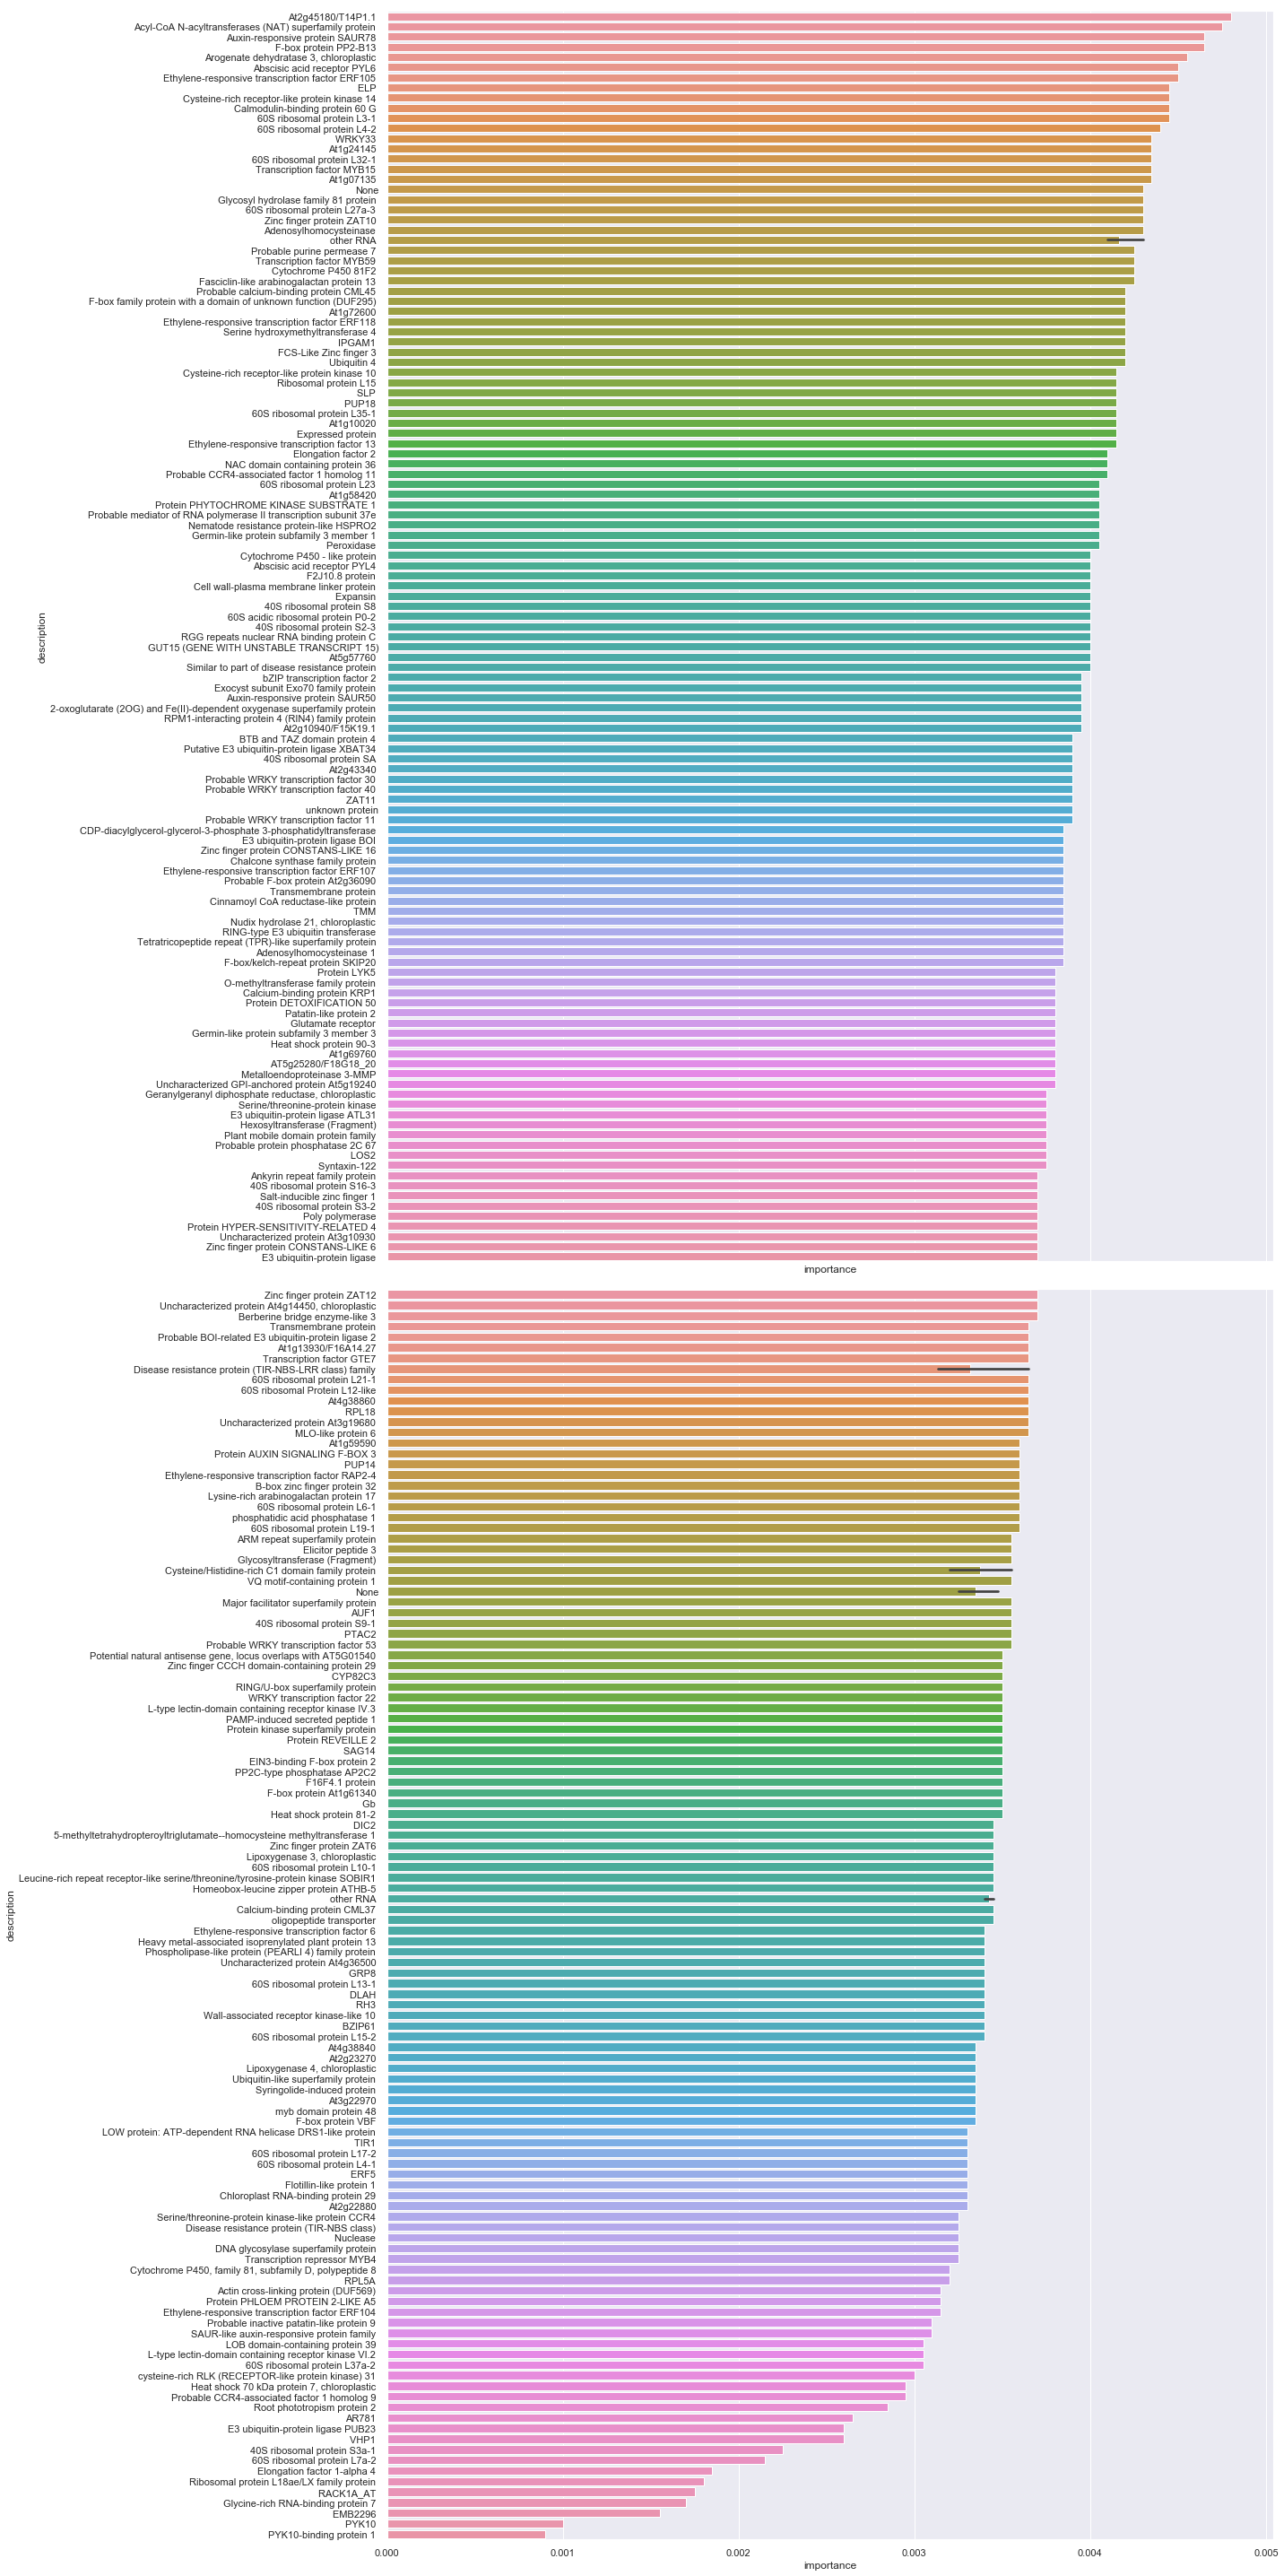
\includegraphics[width=.9\linewidth]{obipy-resources/93e2fbf76ed477962282ae99767b8408de4d3ed9/0fe823d68e2a9c626a5ce7da16dc55177a13d590.png}
\end{center}

\section{Selecting genes for Lym2 at 05hr C/W}
\label{sec:org52daf23}
\subsection{RFE selecting 25 genes}
\label{sec:org944216a}
\begin{minted}[frame=lines,linenos=true,fontfamily=Monaco]{ipython}
from sklearn.feature_selection import RFE, RFECV
from sklearn.linear_model import LogisticRegression

# load data
DE_pairings_05hr = read_xl('/Users/hughesn/PHD/Transcripts/Data/pairings_05hr.xlsx')
sig = DE_pairings_05hr[DE_pairings_05hr['padj'] < 0.05]
sig = sig['log2FoldChange'].sort_values()
locs = sig.index
df = counts.loc[locs][[c for c in counts.columns if ('_05h' in c and 'lym' in c)]].T
df = df.loc[:,~df.columns.duplicated()]
df = df[[c for c in set(df.columns.values)]]
\end{minted}

\begin{minted}[frame=lines,linenos=true,fontfamily=Monaco]{ipython}
# Feature Extraction with RFE
X = df.values
y = [y.rsplit('_',1)[0] for y in df.reset_index()['index']]
# feature extraction
model = LogisticRegression()
rfe = RFE(model, n_features_to_select=25)
fit = rfe.fit(X, y)
print("Num Features: {0}".format(fit.n_features_))
print("Selected Features: {0}".format(fit.support_))
print("Feature Ranking: {0}".format(fit.ranking_))
\end{minted}

Num Features: 25\\
Selected Features: [False False False \ldots{} False False False]\\
Feature Ranking: [3245 1674 3616 \ldots{}   40  172 5357]\\


\begin{minted}[frame=lines,linenos=true,fontfamily=Monaco]{ipython}
genes = []
for r,f in zip(fit.ranking_, df.columns.values):
      if r ==1:
            genes.append(f)
get_gene_names(genes)
\end{minted}

\begin{center}
\begin{tabular}{rlll}
 & incoming & name & description\\
\hline
0 & AT1G79110 & BRG2 & Probable BOI-related E3 ubiquitin-protein ligase 2\\
1 & AT5G60390 & A1 & Elongation factor 1-alpha 4\\
2 & AT1G14540 & PER4 & Peroxidase\\
3 & AT5G61590 & ERF107 & Ethylene-responsive transcription factor ERF107\\
4 & AT1G68520 & COL6 & Zinc finger protein CONSTANS-LIKE 6\\
5 & AT1G56250 & VBF & F-box protein VBF\\
6 & AT2G37430 & ZAT11 & ZAT11\\
7 & AT5G27420 & ATL31 & E3 ubiquitin-protein ligase ATL31\\
8 & AT5G24110 & WRKY30 & Probable WRKY transcription factor 30\\
9 & AT3G02840 & AT3G02840 & ARM repeat superfamily protein\\
10 & AT5G17920 & MS1 & 5-methyltetrahydropteroyltriglutamate--homocysteine methyltransferase 1\\
11 & AT3G09275 & AT3G09275 & None\\
12 & AT4G19700 & BOI & E3 ubiquitin-protein ligase BOI\\
13 & AT3G53460 & CP29 & Chloroplast RNA-binding protein 29\\
14 & AT1G25440 & COL16 & Zinc finger protein CONSTANS-LIKE 16\\
15 & AT5G47230 & ERF5 & ERF5\\
16 & AT1G72520 & LOX4 & Lipoxygenase 4, chloroplastic\\
17 & AT1G56242 & AT1G56242 & other RNA\\
18 & AT5G11140 & AT5G11140 & Phospholipase-like protein (PEARLI 4) family protein\\
19 & AT5G37260 & RVE2 & Protein REVEILLE 2\\
20 & AT2G21660 & RBG7 & Glycine-rich RNA-binding protein 7\\
21 & AT1G56240 & PP2B13 & F-box protein PP2-B13\\
22 & AT1G07160 & AT1G07160 & PP2C-type phosphatase AP2C2\\
23 & AT5G25350 & EBF2 & EIN3-binding F-box protein 2\\
24 & AT1G21120 & AT1G21120 & O-methyltransferase family protein\\
\end{tabular}
\end{center}


\subsubsection{Forest on this RFE set}
\label{sec:orgb60c00f}

\begin{minted}[frame=lines,linenos=true,fontfamily=Monaco]{ipython}
rfe_forest = counts.loc[genes][[c for c in counts.columns if ('_05h' in c and 'lym' in c)]].T
rfe_forest = rfe_forest.loc[:,~rfe_forest.columns.duplicated()]
rfe_forest = rfe_forest[[c for c in set(rfe_forest.columns.values)]]

feat_labels = rfe_forest.columns.values
y = [d.rsplit('_', 1)[0] for d in rfe_forest.index.values]

X_train, X_test, y_train, y_test = train_test_split(rfe_forest.values, y, test_size=1, random_state=42)
forest = RandomForestClassifier(n_estimators=20000, random_state=1, n_jobs=-1)
forest.fit(X_train, y_train)
res = {k: v for k, v in sorted(
    zip(feat_labels, forest.feature_importances_), key=lambda x: x[1], reverse=True)}
res_df = pd.DataFrame(list(res.items()), columns=[
                      'gene', 'importance']).set_index('gene')
names = get_gene_names(list(res_df.index))
res_df = pd.merge(res_df, names, left_index=True, right_on='incoming').rename(
    columns={'incoming': 'gene'}).set_index('gene').sort_values('importance', ascending=False)
res_df
\end{minted}

\begin{center}
\begin{tabular}{lrll}
gene & importance & name & description\\
\hline
AT2G21660 & 0.03965 & RBG7 & Glycine-rich RNA-binding protein 7\\
AT2G37430 & 0.039 & ZAT11 & ZAT11\\
AT1G14540 & 0.03815 & PER4 & Peroxidase\\
AT1G25440 & 0.03755 & COL16 & Zinc finger protein CONSTANS-LIKE 16\\
AT1G21120 & 0.0375 & AT1G21120 & O-methyltransferase family protein\\
AT4G19700 & 0.03745 & BOI & E3 ubiquitin-protein ligase BOI\\
AT1G07160 & 0.03725 & AT1G07160 & PP2C-type phosphatase AP2C2\\
AT3G09275 & 0.03705 & AT3G09275 & None\\
AT5G37260 & 0.037 & RVE2 & Protein REVEILLE 2\\
AT5G25350 & 0.0369 & EBF2 & EIN3-binding F-box protein 2\\
AT1G56242 & 0.03675 & AT1G56242 & other RNA\\
AT5G11140 & 0.0366 & AT5G11140 & Phospholipase-like protein (PEARLI 4) family protein\\
AT3G53460 & 0.03635 & CP29 & Chloroplast RNA-binding protein 29\\
AT1G56250 & 0.03625 & VBF & F-box protein VBF\\
AT5G17920 & 0.0362 & MS1 & 5-methyltetrahydropteroyltriglutamate--homocysteine methyltransferase 1\\
AT1G72520 & 0.0362 & LOX4 & Lipoxygenase 4, chloroplastic\\
AT3G02840 & 0.0361 & AT3G02840 & ARM repeat superfamily protein\\
AT5G60390 & 0.03585 & A1 & Elongation factor 1-alpha 4\\
AT5G47230 & 0.0358 & ERF5 & ERF5\\
AT5G27420 & 0.0356 & ATL31 & E3 ubiquitin-protein ligase ATL31\\
AT5G61590 & 0.03545 & ERF107 & Ethylene-responsive transcription factor ERF107\\
AT1G79110 & 0.035 & BRG2 & Probable BOI-related E3 ubiquitin-protein ligase 2\\
AT1G68520 & 0.03495 & COL6 & Zinc finger protein CONSTANS-LIKE 6\\
AT1G56240 & 0.03425 & PP2B13 & F-box protein PP2-B13\\
AT5G24110 & 0.0341 & WRKY30 & Probable WRKY transcription factor 30\\
\end{tabular}
\end{center}

\begin{minted}[frame=lines,linenos=true,fontfamily=Monaco]{ipython}
fig, ax = plt.subplots(1, figsize=(20,20))
sns.barplot(data=res_df.reset_index(), y='description', x='importance')
plt.tight_layout()
\end{minted}

\begin{verbatim}
<Figure size 1440x1440 with 1 Axes>
\end{verbatim}


\begin{center}
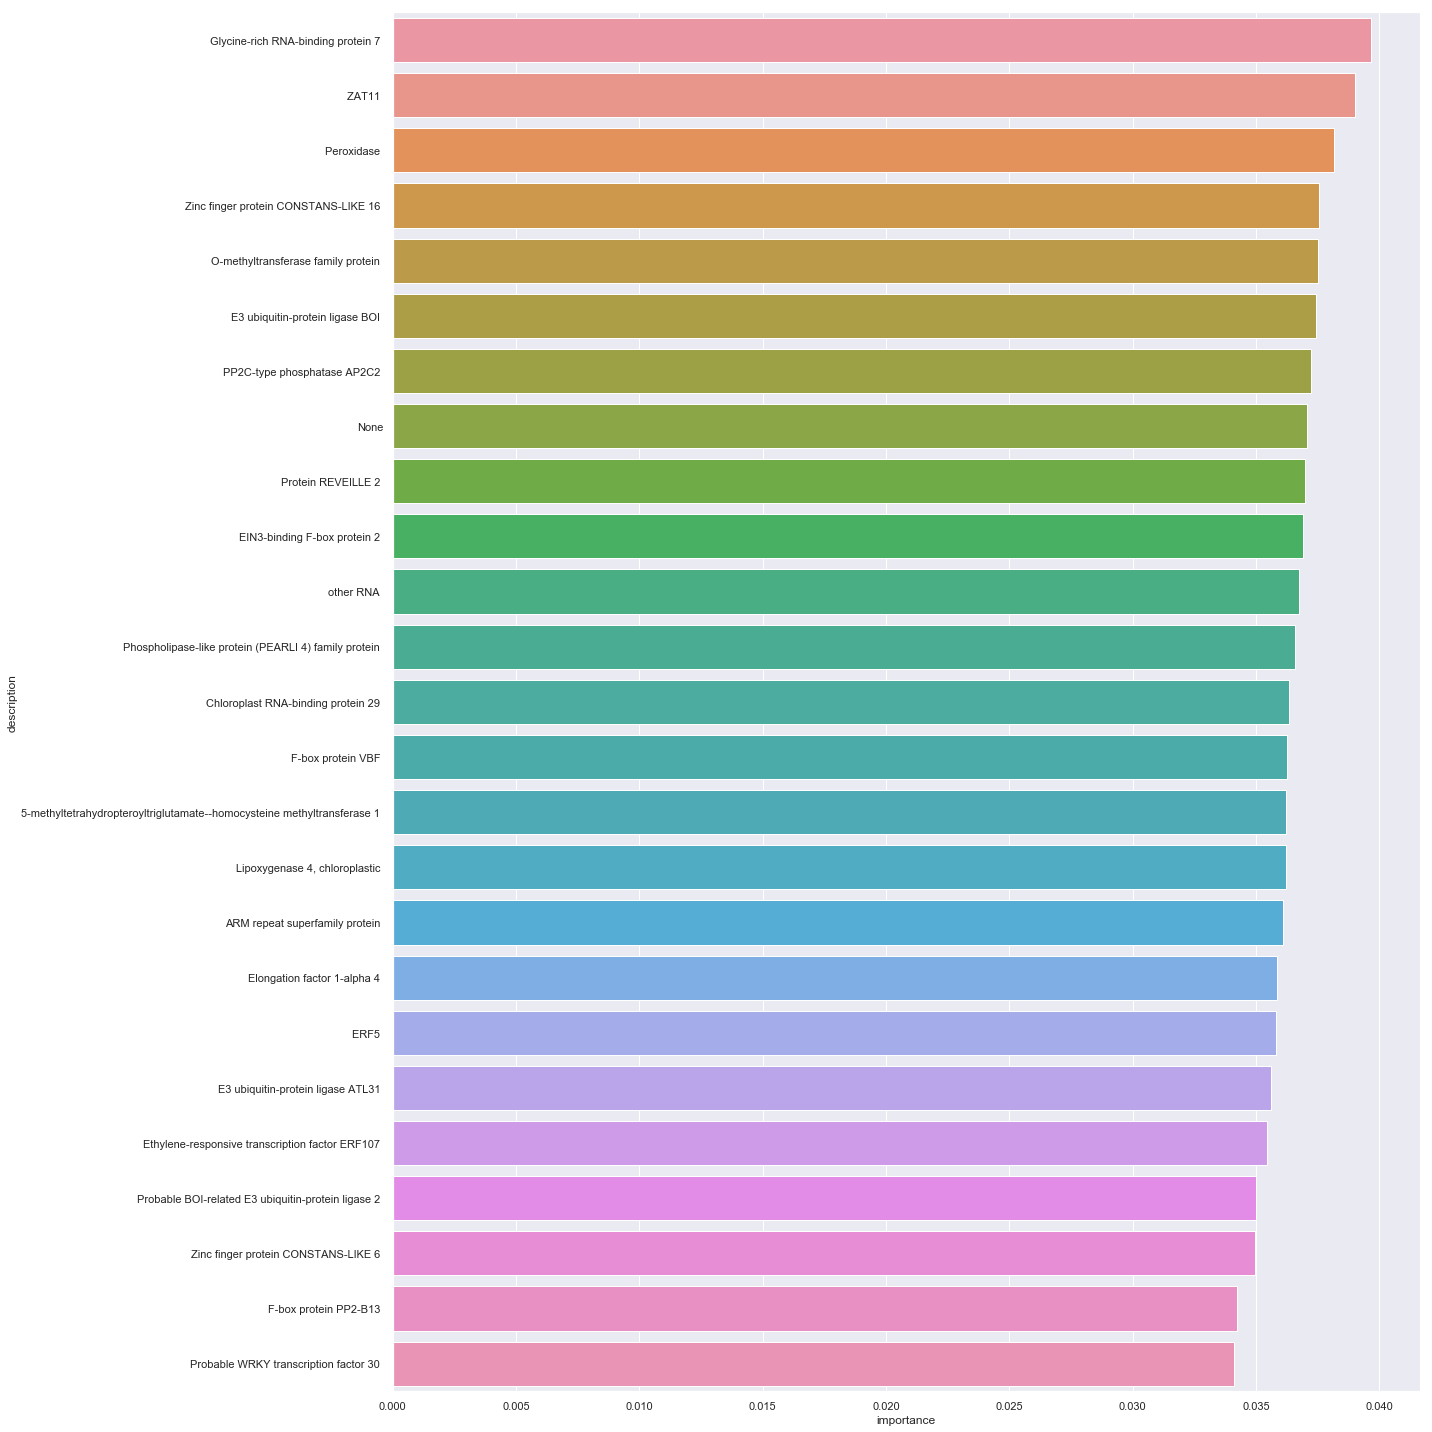
\includegraphics[width=.9\linewidth]{obipy-resources/93e2fbf76ed477962282ae99767b8408de4d3ed9/6c6e3438472c5becb4dd5927f01def5d25fd9d41.png}
\end{center}


\subsection{RFE selecting 250 genes}
\label{sec:orgcf1c68e}
\begin{minted}[frame=lines,linenos=true,fontfamily=Monaco]{ipython}
from sklearn.feature_selection import RFE, RFECV
from sklearn.linear_model import LogisticRegression

# load data
DE_pairings_05hr = read_xl('/Users/hughesn/PHD/Transcripts/Data/pairings_05hr.xlsx')
sig = DE_pairings_05hr[DE_pairings_05hr['padj'] < 0.05]
sig = sig['log2FoldChange'].sort_values()
locs = sig.index
df = counts.loc[locs][[c for c in counts.columns if ('_05h' in c and 'col' in c)]].T
df = df.loc[:,~df.columns.duplicated()]
df = df[[c for c in set(df.columns.values)]]
\end{minted}

\begin{minted}[frame=lines,linenos=true,fontfamily=Monaco]{ipython}
# Feature Extraction with RFE
X = df.values
y = [y.rsplit('_',1)[0] for y in df.reset_index()['index']]
# feature extraction
model = LogisticRegression()
rfe = RFE(model, n_features_to_select=250)
fit = rfe.fit(X, y)
print("Num Features: {0}".format(fit.n_features_))
print("Selected Features: {0}".format(fit.support_))
print("Feature Ranking: {0}".format(fit.ranking_))
\end{minted}

Num Features: 250\\
Selected Features: [False False False \ldots{}  True  True False]\\
Feature Ranking: [ 903  345 2759 \ldots{}    1    1 4498]\\


\begin{minted}[frame=lines,linenos=true,fontfamily=Monaco]{ipython}
genes = []
for r,f in zip(fit.ranking_, df.columns.values):
      if r ==1:
            genes.append(f)
get_gene_names(genes)
\end{minted}



\begin{center}
\begin{tabular}{rlll}
 & incoming & name & description\\
\hline
0 & AT5G59820 & ZAT12 & Zinc finger protein ZAT12\\
1 & AT5G44130 & FLA13 & Fasciclin-like arabinogalactan protein 13\\
2 & AT1G79110 & BRG2 & Probable BOI-related E3 ubiquitin-protein ligase 2\\
3 & AT4G15975 & AT4G15975 & RING/U-box superfamily protein\\
4 & AT5G57760 & AT5G57760 & At5g57760\\
5 & AT4G14365 & XBAT34 & Putative E3 ubiquitin-protein ligase XBAT34\\
6 & AT1G78100 & AT1G78100 & AUF1\\
7 & AT1G78080 & RAP2-4 & Ethylene-responsive transcription factor RAP2-4\\
8 & AT3G16420 & PBP1 & PYK10-binding protein 1\\
9 & AT3G58120 & BZIP61 & BZIP61\\
10 & AT3G22121 & AT3G22121 & other RNA\\
11 & AT2G10940 & AT2G10940 & At2g10940/F15K19.1\\
12 & AT1G74470 & CHLP & Geranylgeranyl diphosphate reductase, chloroplastic\\
13 & AT3G04400 & RPL23A & 60S ribosomal protein L23\\
14 & AT5G25250 & FLOT1 & Flotillin-like protein 1\\
15 & AT5G60390 & A1 & Elongation factor 1-alpha 4\\
16 & AT5G01540 & LECRK62 & L-type lectin-domain containing receptor kinase VI.2\\
17 & AT5G49910 & HSP70-7 & Heat shock 70 kDa protein 7, chloroplastic\\
18 & AT4G14450 & AT4G14450 & Uncharacterized protein At4g14450, chloroplastic\\
19 & AT5G15870 & AT5G15870 & Glycosyl hydrolase family 81 protein\\
20 & AT5G61570 & AT5G61570 & Protein kinase superfamily protein\\
21 & AT3G09260 & BGLU23 & PYK10\\
22 & AT1G80840 & WRKY40 & Probable WRKY transcription factor 40\\
23 & AT5G57220 & CYP81F2 & Cytochrome P450 81F2\\
24 & AT2G25735 & AT2G25735 & Expressed protein\\
25 & AT5G51190 & ERF105 & Ethylene-responsive transcription factor ERF105\\
26 & AT5G41750 & AT5G41750 & Disease resistance protein (TIR-NBS-LRR class) family\\
27 & AT2G27660 & AT2G27660 & Cysteine/Histidine-rich C1 domain family protein\\
28 & AT5G56030 & HSP81-2 & Heat shock protein 81-2\\
29 & AT1G72910 & AT1G72910 & Similar to part of disease resistance protein\\
30 & AT3G59940 & SKIP20 & F-box/kelch-repeat protein SKIP20\\
31 & AT4G24570 & PUMP4 & DIC2\\
32 & AT1G79680 & WAKL10 & Wall-associated receptor kinase-like 10\\
33 & AT3G04840 & RPS3AA & 40S ribosomal protein S3a-1\\
34 & AT4G16370 & ATOPT3 & oligopeptide transporter\\
35 & AT2G35935 & AT2G35935 & None\\
36 & AT5G64905 & PEP3 & Elicitor peptide 3\\
37 & AT1G17147 & VQ1 & VQ motif-containing protein 1\\
38 & AT5G25340 & AT5G25340 & Ubiquitin-like superfamily protein\\
39 & AT4G34760 & SAUR50 & Auxin-responsive protein SAUR50\\
40 & AT1G24140 & 3MMP & Metalloendoproteinase 3-MMP\\
41 & AT1G14540 & PER4 & Peroxidase\\
42 & AT3G23250 & MYB15 & Transcription factor MYB15\\
43 & AT2G36530 & ENO2 & LOS2\\
44 & AT4G23810 & WRKY53 & Probable WRKY transcription factor 53\\
45 & AT2G01180 & ATPAP1 & phosphatidic acid phosphatase 1\\
46 & AT5G59780 & MYB59 & Transcription factor MYB59\\
47 & AT2G45180 & AT2G45180 & At2g45180/T14P1.1\\
48 & AT3G07195 & AT3G07195 & RPM1-interacting protein 4 (RIN4) family protein\\
49 & AT1G48300 & AT1G48300 & unknown protein\\
50 & AT5G28610 & AT5G28610 & LOW protein: ATP-dependent RNA helicase DRS1-like protein\\
51 & AT3G63200 & PLP9 & Probable inactive patatin-like protein 9\\
52 & AT1G07135 & AT1G07135 & At1g07135\\
53 & AT1G09780 & PGM1 & IPGAM1\\
54 & AT3G25520 & ATL5 & RPL5A\\
55 & AT4G38860 & AT4G38860 & At4g38860\\
56 & AT1G12090 & ELP & ELP\\
57 & AT4G29780 & AT4G29780 & Nuclease\\
58 & AT3G49010 & RPL13B & 60S ribosomal protein L13-1\\
59 & AT4G02410 & LECRK43 & L-type lectin-domain containing receptor kinase IV.3\\
60 & AT2G36690 & AT2G36690 & 2-oxoglutarate (2OG) and Fe(II)-dependent oxygenase superfamily protein\\
61 & AT4G14370 & AT4G14370 & Disease resistance protein (TIR-NBS-LRR class) family\\
62 & AT4G38620 & MYB4 & Transcription repressor MYB4\\
63 & AT5G61590 & ERF107 & Ethylene-responsive transcription factor ERF107\\
64 & AT2G41840 & RPS2C & 40S ribosomal protein S2-3\\
65 & AT2G44670 & FLZ3 & FCS-Like Zinc finger 3\\
66 & AT1G05675 & UGT74E1 & Glycosyltransferase (Fragment)\\
67 & AT1G65390 & PP2A5 & Protein PHLOEM PROTEIN 2-LIKE A5\\
68 & AT4G34950 & AT4G34950 & Major facilitator superfamily protein\\
69 & AT5G02500 & MED37E & Probable mediator of RNA polymerase II transcription subunit 37e\\
70 & AT1G68520 & COL6 & Zinc finger protein CONSTANS-LIKE 6\\
71 & AT1G56250 & VBF & F-box protein VBF\\
72 & AT4G18197 & PUP7 & Probable purine permease 7\\
73 & AT5G52050 & DTX50 & Protein DETOXIFICATION 50\\
74 & AT5G20290 & RPS8A & 40S ribosomal protein S8\\
75 & AT1G27730 & ZAT10 & Zinc finger protein ZAT10\\
76 & AT4G13930 & SHM4 & Serine hydroxymethyltransferase 4\\
77 & AT3G44260 & CAF1-9 & Probable CCR4-associated factor 1 homolog 9\\
78 & AT2G37430 & ZAT11 & ZAT11\\
79 & AT5G02870 & RPL4D & 60S ribosomal protein L4-2\\
80 & AT3G09630 & RPL4A & 60S ribosomal protein L4-1\\
81 & AT5G03240 & UBQ3 & Ubiquitin 4\\
82 & AT5G65310 & ATHB-5 & Homeobox-leucine zipper protein ATHB-5\\
83 & AT5G27420 & ATL31 & E3 ubiquitin-protein ligase ATL31\\
84 & AT4G27280 & KRP1 & Calcium-binding protein KRP1\\
85 & AT3G29000 & CML45 & Probable calcium-binding protein CML45\\
86 & AT5G24110 & WRKY30 & Probable WRKY transcription factor 30\\
87 & AT5G61600 & ERF104 & Ethylene-responsive transcription factor ERF104\\
88 & AT5G15845 & AT5G15845 & other RNA\\
89 & AT4G16720 & RPL15A & Ribosomal protein L15\\
90 & AT3G02840 & AT3G02840 & ARM repeat superfamily protein\\
91 & AT5G17920 & MS1 & 5-methyltetrahydropteroyltriglutamate--homocysteine methyltransferase 1\\
92 & AT3G53870 & RPS3B & 40S ribosomal protein S3-2\\
93 & AT1G66090 & AT1G66090 & Disease resistance protein (TIR-NBS class)\\
94 & AT1G67430 & RPL17B & 60S ribosomal protein L17-2\\
95 & AT5G19240 & AT5G19240 & Uncharacterized GPI-anchored protein At5g19240\\
96 & AT3G09275 & AT3G09275 & None\\
97 & AT3G18710 & PUB29 & RING-type E3 ubiquitin transferase\\
98 & AT4G37540 & LBD39 & LOB domain-containing protein 39\\
99 & AT2G02950 & PKS1 & Protein PHYTOCHROME KINASE SUBSTRATE 1\\
100 & AT2G26560 & PLP2 & Patatin-like protein 2\\
101 & AT1G50040 & AT1G50040 & F2J10.8 protein\\
102 & AT1G18540 & RPL6A & 60S ribosomal protein L6-1\\
103 & AT3G05590 & RPL18B & RPL18\\
104 & AT3G62870 & RPL7AB & 60S ribosomal protein L7a-2\\
105 & AT4G01250 & WRKY22 & WRKY transcription factor 22\\
106 & AT2G27820 & ADT3 & Arogenate dehydratase 3, chloroplastic\\
107 & AT1G05575 & AT1G05575 & Transmembrane protein\\
108 & AT1G61360 & AT1G61360 & Serine/threonine-protein kinase\\
109 & AT5G18380 & RPS16C & 40S ribosomal protein S16-3\\
110 & AT1G30370 & AT1G30370 & DLAH\\
111 & AT3G09500 & RPL35A & 60S ribosomal protein L35-1\\
112 & AT2G40000 & HSPRO2 & Nematode resistance protein-like HSPRO2\\
113 & AT1G78170 & AT1G78170 & E3 ubiquitin-protein ligase\\
114 & AT1G59590 & ZCF37 & At1g59590\\
115 & AT4G19700 & BOI & E3 ubiquitin-protein ligase BOI\\
116 & AT5G05300 & AT5G05300 & Gb\\
117 & AT3G53460 & CP29 & Chloroplast RNA-binding protein 29\\
118 & AT1G18080 & RACK1A & RACK1A\_AT\\
119 & AT2G22880 & AT2G22880 & At2g22880\\
120 & AT5G26742 & RH3 & RH3\\
121 & AT2G08475 & AT2G08475 & None\\
122 & AT4G22030 & AT4G22030 & F-box family protein with a domain of unknown function (DUF295)\\
123 & AT1G25440 & COL16 & Zinc finger protein CONSTANS-LIKE 16\\
124 & AT2G32030 & AT2G32030 & Acyl-CoA N-acyltransferases (NAT) superfamily protein\\
125 & AT3G09200 & RPP0B & 60S acidic ribosomal protein P0-2\\
126 & AT1G68550 & ERF118 & Ethylene-responsive transcription factor ERF118\\
127 & AT4G22710 & CYP706A2 & Cytochrome P450 - like protein\\
128 & AT3G22120 & CWLP & Cell wall-plasma membrane linker protein\\
129 & AT3G21150 & BBX32 & B-box zinc finger protein 32\\
130 & AT5G56010 & HSP90-3 & Heat shock protein 90-3\\
131 & AT1G57990 & PUP18 & PUP18\\
132 & AT1G80080 & TMM & TMM\\
133 & AT2G02630 & AT2G02630 & Cysteine/Histidine-rich C1 domain family protein\\
134 & AT4G23220 & CRK14 & Cysteine-rich receptor-like protein kinase 14\\
135 & AT1G26380 & FOX1 & Berberine bridge enzyme-like 3\\
136 & AT3G46130 & ATMYB48 & myb domain protein 48\\
137 & AT5G47230 & ERF5 & ERF5\\
138 & AT1G13930 & AT1G13930 & At1g13930/F16A14.27\\
139 & AT1G24145 & AT1G24145 & At1g24145\\
140 & AT1G50750 & AT1G50750 & Plant mobile domain protein family\\
141 & AT5G25280 & AT5G25280 & AT5g25280/F18G18\_20\\
142 & AT5G47850 & CCR4 & Serine/threonine-protein kinase-like protein CCR4\\
143 & AT1G72520 & LOX4 & Lipoxygenase 4, chloroplastic\\
144 & AT5G41740 & AT5G41740 & Disease resistance protein (TIR-NBS-LRR class) family\\
145 & AT5G44680 & AT5G44680 & DNA glycosylase superfamily protein\\
146 & AT3G03125 & AT3G03125 & None\\
147 & AT1G19020 & AT1G19020 & CDP-diacylglycerol-glycerol-3-phosphate 3-phosphatidyltransferase\\
148 & AT5G52750 & HIPP13 & Heavy metal-associated isoprenylated plant protein 13\\
149 & AT5G20230 & BCB & SAG14\\
150 & AT1G56242 & AT1G56242 & other RNA\\
151 & AT2G31345 & AT2G31345 & Transmembrane protein\\
152 & AT1G10020 & AT1G10020 & At1g10020\\
153 & AT4G11470 & CRK31 & cysteine-rich RLK (RECEPTOR-like protein kinase) 31\\
154 & AT2G38310 & PYL4 & Abscisic acid receptor PYL4\\
155 & AT5G22250 & CAF1-11 & Probable CCR4-associated factor 1 homolog 11\\
156 & AT5G14700 & AT5G14700 & Cinnamoyl CoA reductase-like protein\\
157 & AT1G61340 & AT1G61340 & F-box protein At1g61340\\
158 & AT1G69530 & ATEXPA1 & Expansin\\
159 & AT4G37370 & CYP81D8 & Cytochrome P450, family 81, subfamily D, polypeptide 8\\
160 & AT2G18020 & RPL8A & EMB2296\\
161 & AT2G34480 & AT2G34480 & Ribosomal protein L18ae/LX family protein\\
162 & AT1G20310 & AT1G20310 & Syringolide-induced protein\\
163 & AT5G11140 & AT5G11140 & Phospholipase-like protein (PEARLI 4) family protein\\
164 & AT2G18160 & BZIP2 & bZIP transcription factor 2\\
165 & AT1G72370 & RPSAA & 40S ribosomal protein SA\\
166 & AT5G20630 & GER3 & Germin-like protein subfamily 3 member 3\\
167 & AT3G19680 & AT3G19680 & Uncharacterized protein At3g19680\\
168 & AT3G22970 & AT3G22970 & At3g22970\\
169 & AT5G37260 & RVE2 & Protein REVEILLE 2\\
170 & AT5G04340 & ZAT6 & Zinc finger protein ZAT6\\
171 & AT5G67480 & BT4 & BTB and TAZ domain protein 4\\
172 & AT2G44840 & ERF13 & Ethylene-responsive transcription factor 13\\
173 & AT4G36648 & AT4G36648 & other RNA\\
174 & AT4G17390 & RPL15B & 60S ribosomal protein L15-2\\
175 & AT2G21210 & AT2G21210 & SAUR-like auxin-responsive protein family\\
176 & AT1G73540 & NUDT21 & Nudix hydrolase 21, chloroplastic\\
177 & AT3G01165 & AT3G01165 & None\\
178 & AT3G28340 & GATL10 & Hexosyltransferase (Fragment)\\
179 & AT2G36090 & AT2G36090 & Probable F-box protein At2g36090\\
180 & AT1G61560 & MLO6 & MLO-like protein 6\\
181 & AT2G30520 & RPT2 & Root phototropism protein 2\\
182 & AT1G58420 & AT1G58420 & At1g58420\\
183 & AT3G53430 & RPL12B & 60S ribosomal Protein L12-like\\
184 & AT1G17420 & LOX3 & Lipoxygenase 3, chloroplastic\\
185 & AT1G12820 & AFB3 & Protein AUXIN SIGNALING F-BOX 3\\
186 & AT1G56070 & LOS1 & Elongation factor 2\\
187 & AT2G21660 & RBG7 & Glycine-rich RNA-binding protein 7\\
188 & AT2G18440 & GUT15 & GUT15 (GENE WITH UNSTABLE TRANSCRIPT 15)\\
189 & AT5G15200 & RPS9B & 40S ribosomal protein S9-1\\
190 & AT3G50930 & HSR4 & Protein HYPER-SENSITIVITY-RELATED 4\\
191 & AT4G23180 & CRK10 & Cysteine-rich receptor-like protein kinase 10\\
192 & AT1G19770 & PUP14 & PUP14\\
193 & AT5G26920 & CBP60G & Calmodulin-binding protein 60 G\\
194 & AT5G02760 & AT5G02760 & Probable protein phosphatase 2C 67\\
195 & AT5G47210 & RGGC & RGG repeats nuclear RNA binding protein C\\
196 & AT2G40330 & PYL6 & Abscisic acid receptor PYL6\\
197 & AT1G70600 & RPL27AC & 60S ribosomal protein L27a-3\\
198 & AT2G28000 & CPN60A1 & SLP\\
199 & AT2G31880 & SOBIR1 & Leucine-rich repeat receptor-like serine/threonine/tyrosine-protein kinase SOBIR1\\
200 & AT4G18100 & RPL32A & 60S ribosomal protein L32-1\\
201 & AT4G31550 & WRKY11 & Probable WRKY transcription factor 11\\
202 & AT2G47440 & AT2G47440 & Tetratricopeptide repeat (TPR)-like superfamily protein\\
203 & AT2G23270 & AT2G23270 & At2g23270\\
204 & AT1G76600 & AT1G76600 & Poly polymerase\\
205 & AT2G29110 & ATGLR2.8 & Glutamate receptor\\
206 & AT1G14320 & RPL10A & 60S ribosomal protein L10-1\\
207 & AT1G09690 & RPL21A & 60S ribosomal protein L21-1\\
208 & AT5G59732 & AT5G59732 & other RNA\\
209 & AT1G56240 & PP2B13 & F-box protein PP2-B13\\
210 & AT5G13930 & CHS & Chalcone synthase family protein\\
211 & AT4G31950 & CYP82C3 & CYP82C3\\
212 & AT4G36500 & AT4G36500 & Uncharacterized protein At4g36500\\
213 & AT2G33580 & LYK5 & Protein LYK5\\
214 & AT5G65630 & GTE7 & Transcription factor GTE7\\
215 & AT1G07160 & AT1G07160 & PP2C-type phosphatase AP2C2\\
216 & AT2G38470 & WRKY33 & WRKY33\\
217 & AT4G39260 & RBG8 & GRP8\\
218 & AT4G17490 & ERF6 & Ethylene-responsive transcription factor 6\\
219 & AT2G40140 & CZF1 & Zinc finger CCCH domain-containing protein 29\\
220 & AT5G01542 & AT5G01542 & Potential natural antisense gene, locus overlaps with AT5G01540\\
221 & AT1G43170 & ARP1 & 60S ribosomal protein L3-1\\
222 & AT1G15690 & AVP1 & VHP1\\
223 & AT1G69890 & AT1G69890 & Actin cross-linking protein (DUF569)\\
224 & AT4G38840 & AT4G38840 & At4g38840\\
225 & AT2G17040 & anac036 & NAC domain containing protein 36\\
226 & AT3G10930 & AT3G10930 & Uncharacterized protein At3g10930\\
227 & AT5G25350 & EBF2 & EIN3-binding F-box protein 2\\
228 & AT3G62980 & TIR1 & TIR1\\
229 & AT1G21120 & AT1G21120 & O-methyltransferase family protein\\
230 & AT1G72600 & AT1G72600 & At1g72600\\
231 & AT1G69760 & AT1G69760 & At1g69760\\
232 & AT1G72610 & GLP1 & Germin-like protein subfamily 3 member 1\\
233 & AT4G13940 & SAHH1 & Adenosylhomocysteinase 1\\
234 & AT3G55980 & SZF1 & Salt-inducible zinc finger 1\\
235 & AT5G59730 & ATEXO70H7 & Exocyst subunit Exo70 family protein\\
236 & AT1G72430 & SAUR78 & Auxin-responsive protein SAUR78\\
237 & AT5G42380 & CML37 & Calcium-binding protein CML37\\
238 & AT1G21326 & AT1G21326 & F16F4.1 protein\\
239 & AT3G60245 & RPL37AC & 60S ribosomal protein L37a-2\\
240 & AT2G26530 & AR781 & AR781\\
241 & AT2G24600 & AT2G24600 & Ankyrin repeat family protein\\
242 & AT3G23810 & SAHH2 & Adenosylhomocysteinase\\
243 & AT2G43340 & AT2G43340 & At2g43340\\
244 & AT1G74850 & PTAC2 & PTAC2\\
245 & AT2G35930 & PUB23 & E3 ubiquitin-protein ligase PUB23\\
246 & AT2G23130 & AGP17 & Lysine-rich arabinogalactan protein 17\\
247 & AT4G28460 & PIP1 & PAMP-induced secreted peptide 1\\
248 & AT1G02780 & RPL19A & 60S ribosomal protein L19-1\\
249 & AT3G52400 & SYP122 & Syntaxin-122\\
\end{tabular}
\end{center}


\paragraph{Forest on this RFE}
\label{sec:org714e927}

\begin{minted}[frame=lines,linenos=true,fontfamily=Monaco]{ipython}
rfe_forest = counts.loc[genes][[c for c in counts.columns if ('_05h' in c and 'lym' in c)]].T
rfe_forest = rfe_forest.loc[:,~rfe_forest.columns.duplicated()]
rfe_forest = rfe_forest[[c for c in set(rfe_forest.columns.values)]]

feat_labels = rfe_forest.columns.values
y = [d.rsplit('_', 1)[0] for d in rfe_forest.index.values]

X_train, X_test, y_train, y_test = train_test_split(rfe_forest.values, y, test_size=1, random_state=42)
forest = RandomForestClassifier(n_estimators=20000, random_state=1, n_jobs=-1)
forest.fit(X_train, y_train)
res = {k: v for k, v in sorted(
    zip(feat_labels, forest.feature_importances_), key=lambda x: x[1], reverse=True)}
res_df = pd.DataFrame(list(res.items()), columns=[
                      'gene', 'importance']).set_index('gene')
names = get_gene_names(list(res_df.index))
res_df = pd.merge(res_df, names, left_index=True, right_on='incoming').rename(
    columns={'incoming': 'gene'}).set_index('gene').sort_values('importance', ascending=False)
res_df
\end{minted}

\begin{center}
\begin{tabular}{lrll}
gene & importance & name & description\\
\hline
AT2G32030 & 0.0047 & AT2G32030 & Acyl-CoA N-acyltransferases (NAT) superfamily protein\\
AT1G72430 & 0.0046 & SAUR78 & Auxin-responsive protein SAUR78\\
AT1G56240 & 0.00455 & PP2B13 & F-box protein PP2-B13\\
AT5G26920 & 0.00445 & CBP60G & Calmodulin-binding protein 60 G\\
AT2G40330 & 0.00445 & PYL6 & Abscisic acid receptor PYL6\\
AT4G23220 & 0.0044 & CRK14 & Cysteine-rich receptor-like protein kinase 14\\
AT2G27820 & 0.0044 & ADT3 & Arogenate dehydratase 3, chloroplastic\\
AT1G27730 & 0.00435 & ZAT10 & Zinc finger protein ZAT10\\
AT1G43170 & 0.00435 & ARP1 & 60S ribosomal protein L3-1\\
AT2G21660 & 0.00435 & RBG7 & Glycine-rich RNA-binding protein 7\\
AT5G51190 & 0.00435 & ERF105 & Ethylene-responsive transcription factor ERF105\\
AT5G02870 & 0.0043 & RPL4D & 60S ribosomal protein L4-2\\
AT1G24145 & 0.0043 & AT1G24145 & At1g24145\\
AT2G38470 & 0.0043 & WRKY33 & WRKY33\\
AT5G15870 & 0.0043 & AT5G15870 & Glycosyl hydrolase family 81 protein\\
AT3G01165 & 0.0043 & AT3G01165 & None\\
AT5G59780 & 0.0043 & MYB59 & Transcription factor MYB59\\
AT5G59732 & 0.00425 & AT5G59732 & other RNA\\
AT3G23250 & 0.00425 & MYB15 & Transcription factor MYB15\\
AT4G18100 & 0.00425 & RPL32A & 60S ribosomal protein L32-1\\
AT1G07135 & 0.00425 & AT1G07135 & At1g07135\\
AT3G23810 & 0.00425 & SAHH2 & Adenosylhomocysteinase\\
AT1G70600 & 0.00425 & RPL27AC & 60S ribosomal protein L27a-3\\
AT1G12090 & 0.00425 & ELP & ELP\\
AT4G18197 & 0.00425 & PUP7 & Probable purine permease 7\\
AT1G72600 & 0.0042 & AT1G72600 & At1g72600\\
AT3G04840 & 0.0042 & RPS3AA & 40S ribosomal protein S3a-1\\
AT5G57220 & 0.0042 & CYP81F2 & Cytochrome P450 81F2\\
AT5G44130 & 0.0042 & FLA13 & Fasciclin-like arabinogalactan protein 13\\
AT1G09780 & 0.0042 & PGM1 & IPGAM1\\
AT4G13930 & 0.00415 & SHM4 & Serine hydroxymethyltransferase 4\\
AT2G25735 & 0.00415 & AT2G25735 & Expressed protein\\
AT4G23180 & 0.00415 & CRK10 & Cysteine-rich receptor-like protein kinase 10\\
AT1G68550 & 0.00415 & ERF118 & Ethylene-responsive transcription factor ERF118\\
AT1G58420 & 0.0041 & AT1G58420 & At1g58420\\
AT3G29000 & 0.0041 & CML45 & Probable calcium-binding protein CML45\\
AT3G09500 & 0.0041 & RPL35A & 60S ribosomal protein L35-1\\
AT2G44840 & 0.0041 & ERF13 & Ethylene-responsive transcription factor 13\\
AT4G22030 & 0.0041 & AT4G22030 & F-box family protein with a domain of unknown function (DUF295)\\
AT2G36690 & 0.00405 & AT2G36690 & 2-oxoglutarate (2OG) and Fe(II)-dependent oxygenase superfamily protein\\
AT1G69530 & 0.00405 & ATEXPA1 & Expansin\\
AT4G36648 & 0.00405 & AT4G36648 & other RNA\\
AT2G28000 & 0.00405 & CPN60A1 & SLP\\
AT2G44670 & 0.00405 & FLZ3 & FCS-Like Zinc finger 3\\
AT2G41840 & 0.004 & RPS2C & 40S ribosomal protein S2-3\\
AT2G40000 & 0.004 & HSPRO2 & Nematode resistance protein-like HSPRO2\\
AT1G57990 & 0.004 & PUP18 & PUP18\\
AT1G72610 & 0.004 & GLP1 & Germin-like protein subfamily 3 member 1\\
AT1G14540 & 0.004 & PER4 & Peroxidase\\
AT3G09200 & 0.004 & RPP0B & 60S acidic ribosomal protein P0-2\\
AT1G10020 & 0.004 & AT1G10020 & At1g10020\\
AT4G16720 & 0.004 & RPL15A & Ribosomal protein L15\\
AT5G02500 & 0.004 & MED37E & Probable mediator of RNA polymerase II transcription subunit 37e\\
AT3G22121 & 0.004 & AT3G22121 & other RNA\\
AT3G22120 & 0.004 & CWLP & Cell wall-plasma membrane linker protein\\
AT2G02950 & 0.004 & PKS1 & Protein PHYTOCHROME KINASE SUBSTRATE 1\\
AT2G38310 & 0.004 & PYL4 & Abscisic acid receptor PYL4\\
AT1G72910 & 0.00395 & AT1G72910 & Similar to part of disease resistance protein\\
AT2G18440 & 0.00395 & GUT15 & GUT15 (GENE WITH UNSTABLE TRANSCRIPT 15)\\
AT2G17040 & 0.00395 & anac036 & NAC domain containing protein 36\\
AT2G10940 & 0.00395 & AT2G10940 & At2g10940/F15K19.1\\
AT1G80080 & 0.00395 & TMM & TMM\\
AT5G47210 & 0.00395 & RGGC & RGG repeats nuclear RNA binding protein C\\
AT1G50040 & 0.00395 & AT1G50040 & F2J10.8 protein\\
AT3G62870 & 0.00395 & RPL7AB & 60S ribosomal protein L7a-2\\
AT5G59730 & 0.00395 & ATEXO70H7 & Exocyst subunit Exo70 family protein\\
AT5G22250 & 0.00395 & CAF1-11 & Probable CCR4-associated factor 1 homolog 11\\
AT5G20290 & 0.00395 & RPS8A & 40S ribosomal protein S8\\
AT3G04400 & 0.00395 & RPL23A & 60S ribosomal protein L23\\
AT1G25440 & 0.0039 & COL16 & Zinc finger protein CONSTANS-LIKE 16\\
AT1G48300 & 0.0039 & AT1G48300 & unknown protein\\
AT5G57760 & 0.0039 & AT5G57760 & At5g57760\\
AT1G80840 & 0.0039 & WRKY40 & Probable WRKY transcription factor 40\\
AT4G22710 & 0.0039 & CYP706A2 & Cytochrome P450 - like protein\\
AT1G56070 & 0.0039 & LOS1 & Elongation factor 2\\
AT1G72370 & 0.0039 & RPSAA & 40S ribosomal protein SA\\
AT4G14365 & 0.0039 & XBAT34 & Putative E3 ubiquitin-protein ligase XBAT34\\
AT4G31550 & 0.00385 & WRKY11 & Probable WRKY transcription factor 11\\
AT5G67480 & 0.00385 & BT4 & BTB and TAZ domain protein 4\\
AT2G37430 & 0.00385 & ZAT11 & ZAT11\\
AT2G47440 & 0.00385 & AT2G47440 & Tetratricopeptide repeat (TPR)-like superfamily protein\\
AT3G18710 & 0.00385 & PUB29 & RING-type E3 ubiquitin transferase\\
AT2G18160 & 0.00385 & BZIP2 & bZIP transcription factor 2\\
AT3G59940 & 0.00385 & SKIP20 & F-box/kelch-repeat protein SKIP20\\
AT5G24110 & 0.00385 & WRKY30 & Probable WRKY transcription factor 30\\
AT2G36090 & 0.00385 & AT2G36090 & Probable F-box protein At2g36090\\
AT4G34760 & 0.00385 & SAUR50 & Auxin-responsive protein SAUR50\\
AT5G52050 & 0.00385 & DTX50 & Protein DETOXIFICATION 50\\
AT5G25280 & 0.0038 & AT5G25280 & AT5g25280/F18G18\_20\\
AT3G52400 & 0.0038 & SYP122 & Syntaxin-122\\
AT1G73540 & 0.0038 & NUDT21 & Nudix hydrolase 21, chloroplastic\\
AT1G24140 & 0.0038 & 3MMP & Metalloendoproteinase 3-MMP\\
AT2G31345 & 0.0038 & AT2G31345 & Transmembrane protein\\
AT5G61590 & 0.0038 & ERF107 & Ethylene-responsive transcription factor ERF107\\
AT5G27420 & 0.0038 & ATL31 & E3 ubiquitin-protein ligase ATL31\\
AT5G13930 & 0.0038 & CHS & Chalcone synthase family protein\\
AT1G50750 & 0.00375 & AT1G50750 & Plant mobile domain protein family\\
AT3G10930 & 0.00375 & AT3G10930 & Uncharacterized protein At3g10930\\
AT2G43340 & 0.00375 & AT2G43340 & At2g43340\\
AT3G07195 & 0.00375 & AT3G07195 & RPM1-interacting protein 4 (RIN4) family protein\\
AT2G36530 & 0.00375 & ENO2 & LOS2\\
AT1G68520 & 0.00375 & COL6 & Zinc finger protein CONSTANS-LIKE 6\\
AT2G33580 & 0.00375 & LYK5 & Protein LYK5\\
AT3G28340 & 0.00375 & GATL10 & Hexosyltransferase (Fragment)\\
AT1G79110 & 0.00375 & BRG2 & Probable BOI-related E3 ubiquitin-protein ligase 2\\
AT4G27280 & 0.00375 & KRP1 & Calcium-binding protein KRP1\\
AT1G19020 & 0.00375 & AT1G19020 & CDP-diacylglycerol-glycerol-3-phosphate 3-phosphatidyltransferase\\
AT1G21120 & 0.00375 & AT1G21120 & O-methyltransferase family protein\\
AT4G13940 & 0.0037 & SAHH1 & Adenosylhomocysteinase 1\\
AT1G61560 & 0.0037 & MLO6 & MLO-like protein 6\\
AT5G19240 & 0.0037 & AT5G19240 & Uncharacterized GPI-anchored protein At5g19240\\
AT5G65630 & 0.0037 & GTE7 & Transcription factor GTE7\\
AT5G59820 & 0.0037 & ZAT12 & Zinc finger protein ZAT12\\
AT2G26560 & 0.0037 & PLP2 & Patatin-like protein 2\\
AT4G19700 & 0.0037 & BOI & E3 ubiquitin-protein ligase BOI\\
AT1G61360 & 0.0037 & AT1G61360 & Serine/threonine-protein kinase\\
AT1G69760 & 0.00365 & AT1G69760 & At1g69760\\
AT1G78170 & 0.00365 & AT1G78170 & E3 ubiquitin-protein ligase\\
AT5G14700 & 0.00365 & AT5G14700 & Cinnamoyl CoA reductase-like protein\\
AT2G29110 & 0.00365 & ATGLR2.8 & Glutamate receptor\\
AT3G21150 & 0.00365 & BBX32 & B-box zinc finger protein 32\\
AT5G02760 & 0.00365 & AT5G02760 & Probable protein phosphatase 2C 67\\
AT4G14450 & 0.00365 & AT4G14450 & Uncharacterized protein At4g14450, chloroplastic\\
AT5G18380 & 0.00365 & RPS16C & 40S ribosomal protein S16-3\\
AT2G24600 & 0.00365 & AT2G24600 & Ankyrin repeat family protein\\
AT3G50930 & 0.00365 & HSR4 & Protein HYPER-SENSITIVITY-RELATED 4\\
AT3G55980 & 0.00365 & SZF1 & Salt-inducible zinc finger 1\\
AT1G74470 & 0.00365 & CHLP & Geranylgeranyl diphosphate reductase, chloroplastic\\
AT3G53870 & 0.00365 & RPS3B & 40S ribosomal protein S3-2\\
AT4G14370 & 0.0036 & AT4G14370 & Disease resistance protein (TIR-NBS-LRR class) family\\
AT1G02780 & 0.0036 & RPL19A & 60S ribosomal protein L19-1\\
AT1G18540 & 0.0036 & RPL6A & 60S ribosomal protein L6-1\\
AT5G56010 & 0.0036 & HSP90-3 & Heat shock protein 90-3\\
AT1G26380 & 0.0036 & FOX1 & Berberine bridge enzyme-like 3\\
AT1G76600 & 0.0036 & AT1G76600 & Poly polymerase\\
AT1G12820 & 0.0036 & AFB3 & Protein AUXIN SIGNALING F-BOX 3\\
AT3G19680 & 0.00355 & AT3G19680 & Uncharacterized protein At3g19680\\
AT2G01180 & 0.00355 & ATPAP1 & phosphatidic acid phosphatase 1\\
AT1G05575 & 0.00355 & AT1G05575 & Transmembrane protein\\
AT3G02840 & 0.00355 & AT3G02840 & ARM repeat superfamily protein\\
AT3G05590 & 0.00355 & RPL18B & RPL18\\
AT4G38860 & 0.00355 & AT4G38860 & At4g38860\\
AT3G53430 & 0.00355 & RPL12B & 60S ribosomal Protein L12-like\\
AT1G78100 & 0.00355 & AT1G78100 & AUF1\\
AT5G20630 & 0.00355 & GER3 & Germin-like protein subfamily 3 member 3\\
AT5G01542 & 0.00355 & AT5G01542 & Potential natural antisense gene, locus overlaps with AT5G01540\\
AT1G78080 & 0.00355 & RAP2-4 & Ethylene-responsive transcription factor RAP2-4\\
AT1G19770 & 0.00355 & PUP14 & PUP14\\
AT1G13930 & 0.00355 & AT1G13930 & At1g13930/F16A14.27\\
AT5G64905 & 0.00355 & PEP3 & Elicitor peptide 3\\
AT1G59590 & 0.00355 & ZCF37 & At1g59590\\
AT5G65310 & 0.0035 & ATHB-5 & Homeobox-leucine zipper protein ATHB-5\\
AT1G07160 & 0.0035 & AT1G07160 & PP2C-type phosphatase AP2C2\\
AT5G25350 & 0.0035 & EBF2 & EIN3-binding F-box protein 2\\
AT2G23130 & 0.0035 & AGP17 & Lysine-rich arabinogalactan protein 17\\
AT5G56030 & 0.0035 & HSP81-2 & Heat shock protein 81-2\\
AT1G05675 & 0.0035 & UGT74E1 & Glycosyltransferase (Fragment)\\
AT4G01250 & 0.0035 & WRKY22 & WRKY transcription factor 22\\
AT5G61570 & 0.0035 & AT5G61570 & Protein kinase superfamily protein\\
AT1G09690 & 0.0035 & RPL21A & 60S ribosomal protein L21-1\\
AT1G17147 & 0.0035 & VQ1 & VQ motif-containing protein 1\\
AT2G02630 & 0.0035 & AT2G02630 & Cysteine/Histidine-rich C1 domain family protein\\
AT1G74850 & 0.00345 & PTAC2 & PTAC2\\
AT1G61340 & 0.00345 & AT1G61340 & F-box protein At1g61340\\
AT1G21326 & 0.00345 & AT1G21326 & F16F4.1 protein\\
AT5G37260 & 0.00345 & RVE2 & Protein REVEILLE 2\\
AT5G42380 & 0.00345 & CML37 & Calcium-binding protein CML37\\
AT4G23810 & 0.00345 & WRKY53 & Probable WRKY transcription factor 53\\
AT5G20230 & 0.00345 & BCB & SAG14\\
AT2G34480 & 0.00345 & AT2G34480 & Ribosomal protein L18ae/LX family protein\\
AT4G28460 & 0.00345 & PIP1 & PAMP-induced secreted peptide 1\\
AT1G30370 & 0.00345 & AT1G30370 & DLAH\\
AT4G16370 & 0.00345 & ATOPT3 & oligopeptide transporter\\
AT4G39260 & 0.00345 & RBG8 & GRP8\\
AT4G31950 & 0.00345 & CYP82C3 & CYP82C3\\
AT2G08475 & 0.00345 & AT2G08475 & None\\
AT4G34950 & 0.0034 & AT4G34950 & Major facilitator superfamily protein\\
AT5G15200 & 0.0034 & RPS9B & 40S ribosomal protein S9-1\\
AT3G58120 & 0.0034 & BZIP61 & BZIP61\\
AT5G15845 & 0.0034 & AT5G15845 & other RNA\\
AT1G56242 & 0.0034 & AT1G56242 & other RNA\\
AT3G03125 & 0.0034 & AT3G03125 & None\\
AT2G40140 & 0.0034 & CZF1 & Zinc finger CCCH domain-containing protein 29\\
AT5G04340 & 0.0034 & ZAT6 & Zinc finger protein ZAT6\\
AT5G11140 & 0.0034 & AT5G11140 & Phospholipase-like protein (PEARLI 4) family protein\\
AT5G17920 & 0.0034 & MS1 & 5-methyltetrahydropteroyltriglutamate--homocysteine methyltransferase 1\\
AT5G52750 & 0.0034 & HIPP13 & Heavy metal-associated isoprenylated plant protein 13\\
AT5G05300 & 0.00335 & AT5G05300 & Gb\\
AT3G46130 & 0.00335 & ATMYB48 & myb domain protein 48\\
AT5G25250 & 0.00335 & FLOT1 & Flotillin-like protein 1\\
AT1G79680 & 0.00335 & WAKL10 & Wall-associated receptor kinase-like 10\\
AT5G26742 & 0.00335 & RH3 & RH3\\
AT2G31880 & 0.00335 & SOBIR1 & Leucine-rich repeat receptor-like serine/threonine/tyrosine-protein kinase SOBIR1\\
AT4G02410 & 0.00335 & LECRK43 & L-type lectin-domain containing receptor kinase IV.3\\
AT3G49010 & 0.00335 & RPL13B & 60S ribosomal protein L13-1\\
AT4G17490 & 0.00335 & ERF6 & Ethylene-responsive transcription factor 6\\
AT1G14320 & 0.00335 & RPL10A & 60S ribosomal protein L10-1\\
AT1G17420 & 0.00335 & LOX3 & Lipoxygenase 3, chloroplastic\\
AT3G62980 & 0.00335 & TIR1 & TIR1\\
AT4G17390 & 0.0033 & RPL15B & 60S ribosomal protein L15-2\\
AT5G47230 & 0.0033 & ERF5 & ERF5\\
AT3G22970 & 0.0033 & AT3G22970 & At3g22970\\
AT1G56250 & 0.0033 & VBF & F-box protein VBF\\
AT1G20310 & 0.0033 & AT1G20310 & Syringolide-induced protein\\
AT3G09275 & 0.0033 & AT3G09275 & None\\
AT1G67430 & 0.0033 & RPL17B & 60S ribosomal protein L17-2\\
AT4G24570 & 0.0033 & PUMP4 & DIC2\\
AT4G15975 & 0.0033 & AT4G15975 & RING/U-box superfamily protein\\
AT4G38840 & 0.0033 & AT4G38840 & At4g38840\\
AT4G36500 & 0.0033 & AT4G36500 & Uncharacterized protein At4g36500\\
AT1G72520 & 0.0033 & LOX4 & Lipoxygenase 4, chloroplastic\\
AT5G47850 & 0.0033 & CCR4 & Serine/threonine-protein kinase-like protein CCR4\\
AT5G28610 & 0.00325 & AT5G28610 & LOW protein: ATP-dependent RNA helicase DRS1-like protein\\
AT1G66090 & 0.00325 & AT1G66090 & Disease resistance protein (TIR-NBS class)\\
AT5G25340 & 0.00325 & AT5G25340 & Ubiquitin-like superfamily protein\\
AT4G38620 & 0.00325 & MYB4 & Transcription repressor MYB4\\
AT4G29780 & 0.0032 & AT4G29780 & Nuclease\\
AT5G44680 & 0.0032 & AT5G44680 & DNA glycosylase superfamily protein\\
AT2G22880 & 0.0032 & AT2G22880 & At2g22880\\
AT3G09260 & 0.0032 & BGLU23 & PYK10\\
AT5G60390 & 0.0032 & A1 & Elongation factor 1-alpha 4\\
AT3G09630 & 0.0032 & RPL4A & 60S ribosomal protein L4-1\\
AT2G27660 & 0.0032 & AT2G27660 & Cysteine/Histidine-rich C1 domain family protein\\
AT2G23270 & 0.0032 & AT2G23270 & At2g23270\\
AT2G18020 & 0.00315 & RPL8A & EMB2296\\
AT1G65390 & 0.00315 & PP2A5 & Protein PHLOEM PROTEIN 2-LIKE A5\\
AT5G41740 & 0.00315 & AT5G41740 & Disease resistance protein (TIR-NBS-LRR class) family\\
AT4G37370 & 0.0031 & CYP81D8 & Cytochrome P450, family 81, subfamily D, polypeptide 8\\
AT2G35935 & 0.0031 & AT2G35935 & None\\
AT3G60245 & 0.0031 & RPL37AC & 60S ribosomal protein L37a-2\\
AT2G21210 & 0.0031 & AT2G21210 & SAUR-like auxin-responsive protein family\\
AT5G61600 & 0.0031 & ERF104 & Ethylene-responsive transcription factor ERF104\\
AT3G53460 & 0.0031 & CP29 & Chloroplast RNA-binding protein 29\\
AT3G25520 & 0.00305 & ATL5 & RPL5A\\
AT5G01540 & 0.00305 & LECRK62 & L-type lectin-domain containing receptor kinase VI.2\\
AT3G63200 & 0.00305 & PLP9 & Probable inactive patatin-like protein 9\\
AT5G41750 & 0.00305 & AT5G41750 & Disease resistance protein (TIR-NBS-LRR class) family\\
AT1G69890 & 0.003 & AT1G69890 & Actin cross-linking protein (DUF569)\\
AT4G37540 & 0.003 & LBD39 & LOB domain-containing protein 39\\
AT4G11470 & 0.00295 & CRK31 & cysteine-rich RLK (RECEPTOR-like protein kinase) 31\\
AT1G18080 & 0.00295 & RACK1A & RACK1A\_AT\\
AT3G16420 & 0.00295 & PBP1 & PYK10-binding protein 1\\
AT5G49910 & 0.0029 & HSP70-7 & Heat shock 70 kDa protein 7, chloroplastic\\
AT3G44260 & 0.00285 & CAF1-9 & Probable CCR4-associated factor 1 homolog 9\\
AT2G30520 & 0.00285 & RPT2 & Root phototropism protein 2\\
AT2G35930 & 0.0027 & PUB23 & E3 ubiquitin-protein ligase PUB23\\
AT2G26530 & 0.0027 & AR781 & AR781\\
AT1G15690 & 0.0026 & AVP1 & VHP1\\
AT2G45180 & 0.00245 & AT2G45180 & At2g45180/T14P1.1\\
AT5G03240 & 0.00195 & UBQ3 & Ubiquitin 4\\
\end{tabular}
\end{center}

\begin{minted}[frame=lines,linenos=true,fontfamily=Monaco]{ipython}
fig, ax = plt.subplots(2,1, figsize=(20,40), sharex=True)
res_df=res_df.sort_values(by='importance', ascending=False)
size = len(res_df)
sns.barplot(data=res_df.reset_index().iloc[:int(size/2)], y='description', x='importance', ax=ax[0])
sns.barplot(data=res_df.reset_index().iloc[int(size/2):], y='description', x='importance', ax=ax[1])
fig.tight_layout()
\end{minted}

\begin{verbatim}
<Figure size 1440x2880 with 2 Axes>
\end{verbatim}


\begin{center}
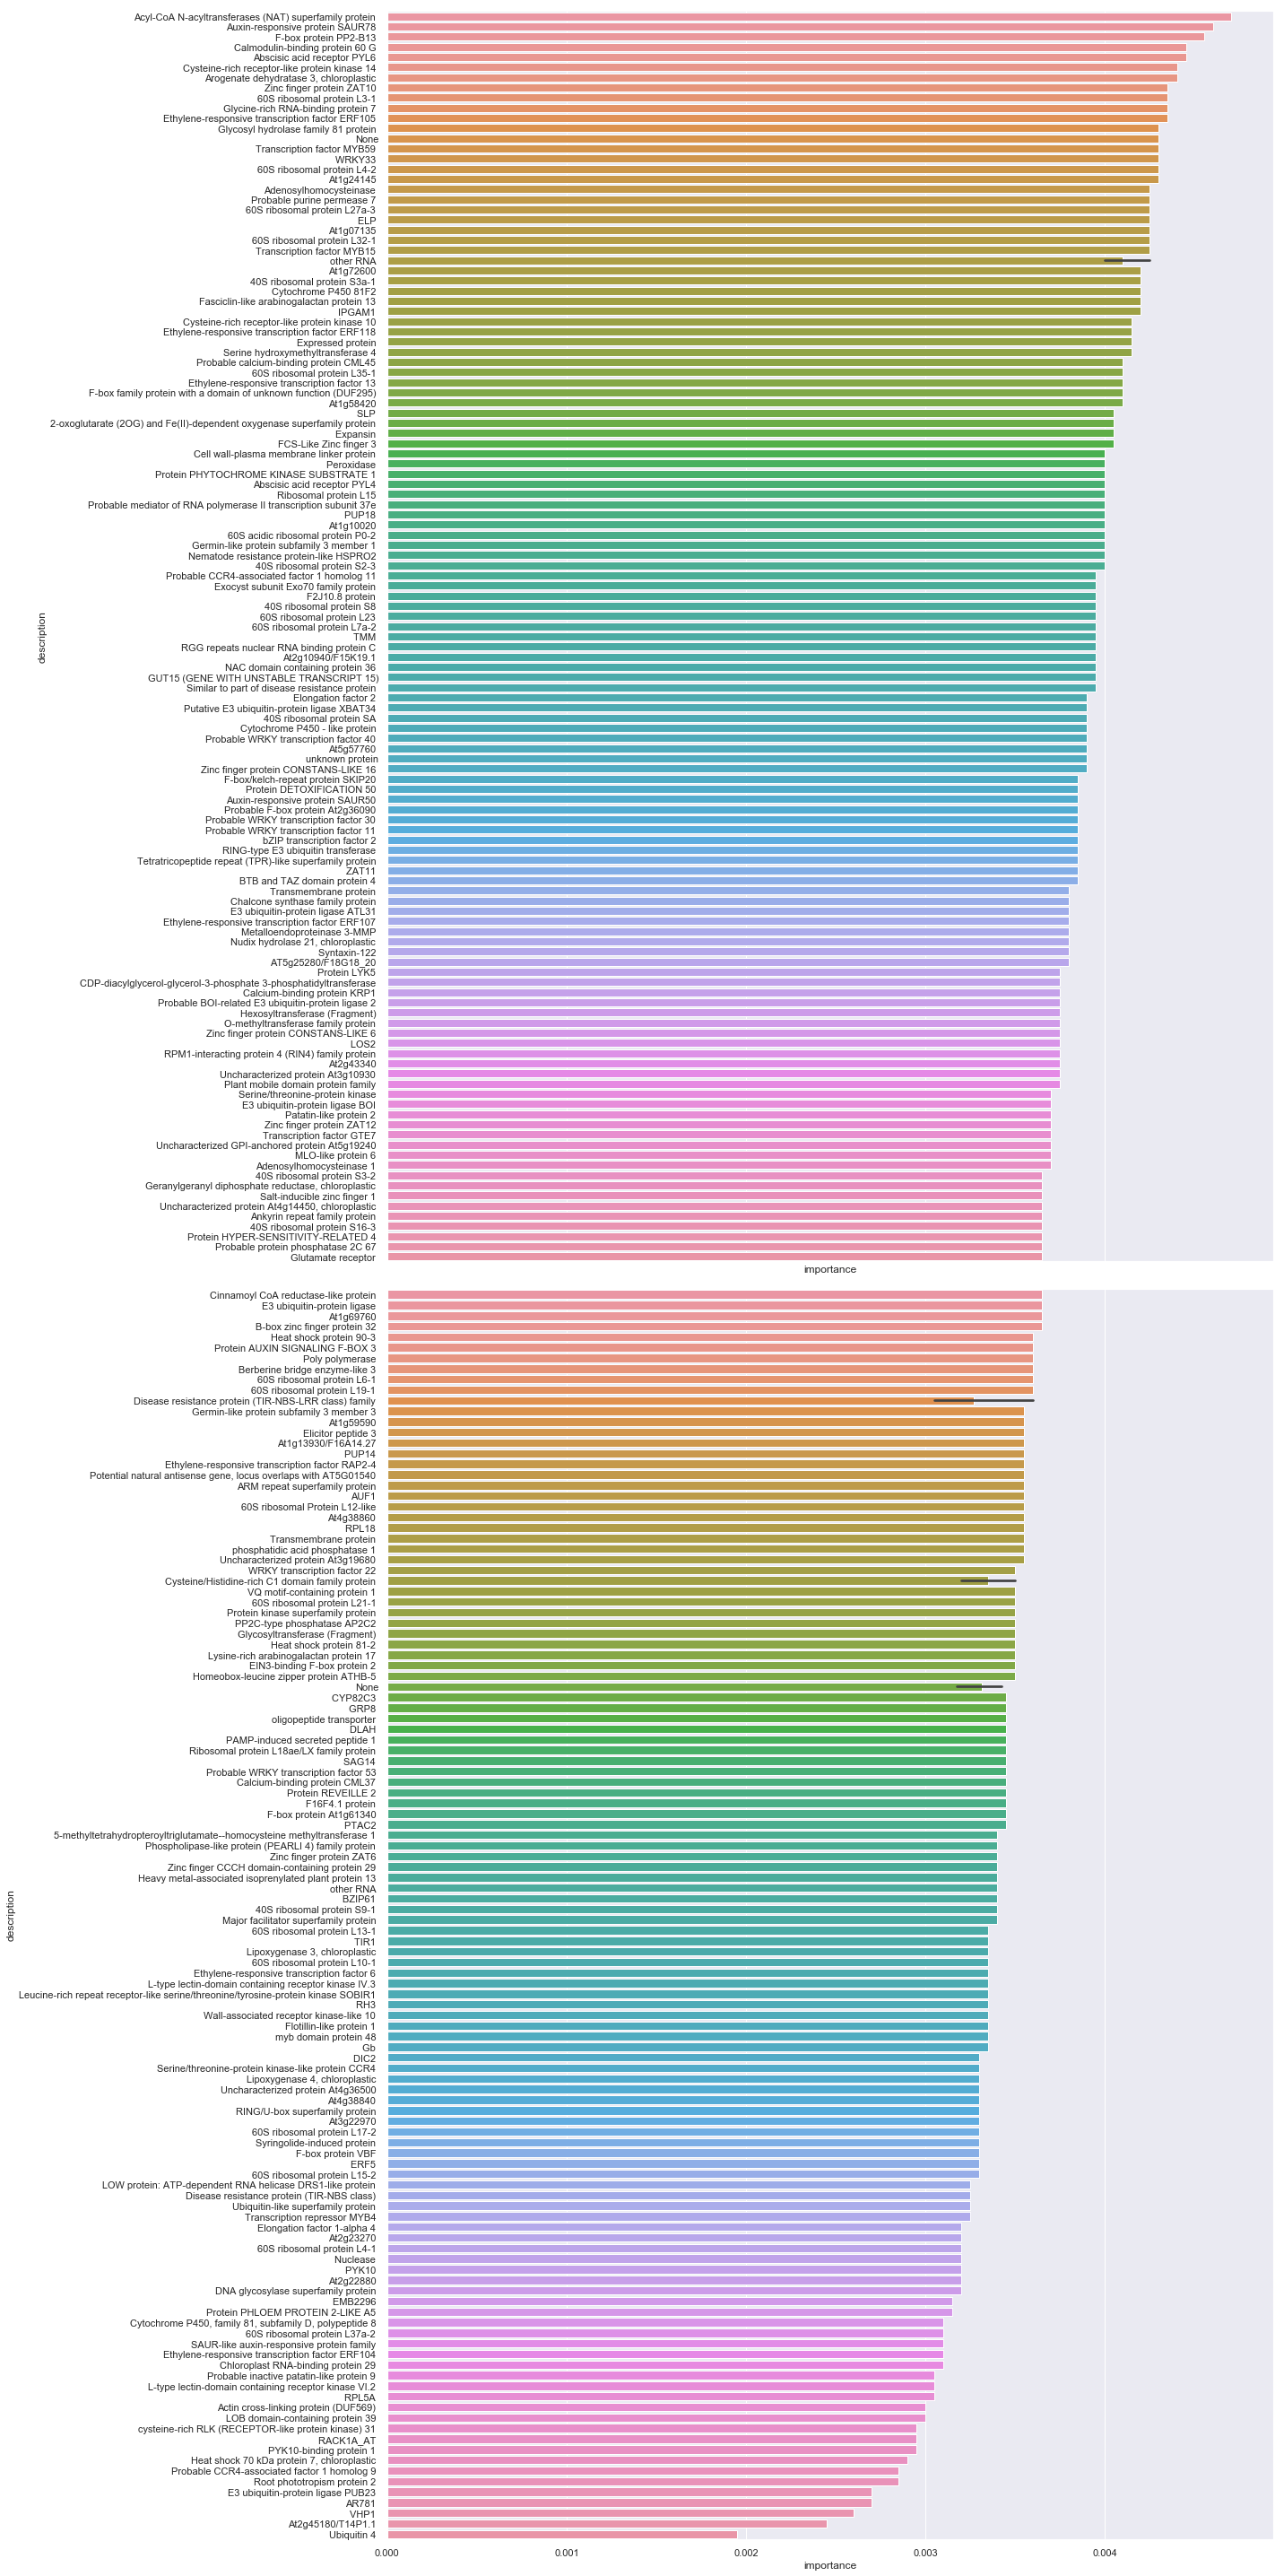
\includegraphics[width=.9\linewidth]{obipy-resources/93e2fbf76ed477962282ae99767b8408de4d3ed9/247f3a8ca81edfa728b6d12c14378ecb5bd32480.png}
\end{center}

\section{Selecting genes for cerk at 05hr C/W}
\label{sec:orga881dd9}
\subsection{RFE selecting 25 genes}
\label{sec:org5888335}
\begin{minted}[frame=lines,linenos=true,fontfamily=Monaco]{ipython}

from sklearn.feature_selection import RFE, RFECV
from sklearn.linear_model import LogisticRegression

# load data
DE_pairings_05hr = read_xl('/Users/hughesn/PHD/Transcripts/Data/pairings_05hr.xlsx')
sig = DE_pairings_05hr[DE_pairings_05hr['padj'] < 0.05]
sig = sig['log2FoldChange'].sort_values()
locs = sig.index
df = counts.loc[locs][[c for c in counts.columns if ('_05h' in c and 'cer' in c)]].T
df = df.loc[:,~df.columns.duplicated()]
df = df[[c for c in set(df.columns.values)]]
\end{minted}

\begin{minted}[frame=lines,linenos=true,fontfamily=Monaco]{ipython}
# Feature Extraction with RFE
X = df.values
y = [y.rsplit('_',1)[0] for y in df.reset_index()['index']]
# feature extraction
model = LogisticRegression()
rfe = RFE(model, n_features_to_select=25)
fit = rfe.fit(X, y)
print("Num Features: {0}".format(fit.n_features_))
print("Selected Features: {0}".format(fit.support_))
print("Feature Ranking: {0}".format(fit.ranking_))
\end{minted}

Num Features: 25\\
Selected Features: [False False False \ldots{} False False False]\\
Feature Ranking: [4396 2028 2192 \ldots{} 6054  220 3792]\\


\begin{minted}[frame=lines,linenos=true,fontfamily=Monaco]{ipython}
genes = []
for r,f in zip(fit.ranking_, df.columns.values):
      if r ==1:
            genes.append(f)
get_gene_names(genes)
\end{minted}

\begin{center}
\begin{tabular}{rlll}
 & incoming & name & description\\
\hline
0 & AT2G44578 & AT2G44578 & RING/U-box superfamily protein\\
1 & AT1G48740 & AT1G48740 & 2-oxoglutarate (2OG) and Fe(II)-dependent oxygenase superfamily protein\\
2 & AT5G42800 & DFRA & Dihydroflavonol reductase\\
3 & AT3G13020 & AT3G13020 & HAT transposon superfamily protein\\
4 & AT1G07135 & AT1G07135 & At1g07135\\
5 & AT3G63095 & AT3G63095 & Tetratricopeptide repeat (TPR)-like superfamily protein\\
6 & AT4G01360 & AT4G01360 & BPS1-like protein\\
7 & AT5G05250 & AT5G05250 & AT5g05250/K18I23\_5\\
8 & AT4G23680 & AT4G23680 & AT4g23680/F9D16\_150\\
9 & AT5G59320 & LTP3 & Non-specific lipid-transfer protein 3\\
10 & AT3G21080 & AT3G21080 & ABC transporter-like protein\\
11 & AT5G05300 & AT5G05300 & Gb\\
12 & AT1G30135 & TIFY5A & Protein TIFY 5A\\
13 & AT1G56242 & AT1G56242 & other RNA\\
14 & AT3G60415 & AT3G60415 & At3g60420\\
15 & AT3G09440 & HSP70-3 & Heat shock protein 70 (Hsp 70) family protein\\
16 & AT5G50790 & SWEET10 & Bidirectional sugar transporter SWEET10\\
17 & AT2G22860 & PSK2 & Phytosulfokines 2\\
18 & AT3G60690 & AT3G60690 & AT3g60690/T4C21\_100\\
19 & AT4G17490 & ERF6 & Ethylene-responsive transcription factor 6\\
20 & AT3G48080 & EDS1B & Protein EDS1B\\
21 & AT4G35180 & LHT7 & Lysine histidine transporter-like 7\\
22 & AT3G49900 & AT3G49900 & Phototropic-responsive NPH3 family protein\\
23 & AT5G47500 & PME68 & Probable pectinesterase 68\\
24 & AT5G24530 & DMR6 & Protein DOWNY MILDEW RESISTANCE 6\\
\end{tabular}
\end{center}


\subsubsection{Forest on this RFE set}
\label{sec:org20eabc1}

\begin{minted}[frame=lines,linenos=true,fontfamily=Monaco]{ipython}
rfe_forest = counts.loc[genes][[c for c in counts.columns if ('_05h' in c and 'cer' in c)]].T
rfe_forest = rfe_forest.loc[:,~rfe_forest.columns.duplicated()]
rfe_forest = rfe_forest[[c for c in set(rfe_forest.columns.values)]]

feat_labels = rfe_forest.columns.values
y = [d.rsplit('_', 1)[0] for d in rfe_forest.index.values]

X_train, X_test, y_train, y_test = train_test_split(rfe_forest.values, y, test_size=1, random_state=42)
forest = RandomForestClassifier(n_estimators=20000, random_state=1, n_jobs=-1)
forest.fit(X_train, y_train)
res = {k: v for k, v in sorted(
    zip(feat_labels, forest.feature_importances_), key=lambda x: x[1], reverse=True)}
res_df = pd.DataFrame(list(res.items()), columns=[
                      'gene', 'importance']).set_index('gene')
names = get_gene_names(list(res_df.index))
res_df = pd.merge(res_df, names, left_index=True, right_on='incoming').rename(
    columns={'incoming': 'gene'}).set_index('gene').sort_values('importance', ascending=False)
res_df
\end{minted}

\begin{center}
\begin{tabular}{lrll}
gene & importance & name & description\\
\hline
AT4G35180 & 0.0426 & LHT7 & Lysine histidine transporter-like 7\\
AT5G05250 & 0.0412 & AT5G05250 & AT5g05250/K18I23\_5\\
AT4G01360 & 0.0406 & AT4G01360 & BPS1-like protein\\
AT1G30135 & 0.0404 & TIFY5A & Protein TIFY 5A\\
AT5G47500 & 0.04035 & PME68 & Probable pectinesterase 68\\
AT5G59320 & 0.0403 & LTP3 & Non-specific lipid-transfer protein 3\\
AT3G13020 & 0.04005 & AT3G13020 & HAT transposon superfamily protein\\
AT1G56242 & 0.0398 & AT1G56242 & other RNA\\
AT5G24530 & 0.03975 & DMR6 & Protein DOWNY MILDEW RESISTANCE 6\\
AT4G17490 & 0.0394 & ERF6 & Ethylene-responsive transcription factor 6\\
AT5G50790 & 0.03935 & SWEET10 & Bidirectional sugar transporter SWEET10\\
AT4G23680 & 0.03925 & AT4G23680 & AT4g23680/F9D16\_150\\
AT1G48740 & 0.039 & AT1G48740 & 2-oxoglutarate (2OG) and Fe(II)-dependent oxygenase superfamily protein\\
AT2G22860 & 0.039 & PSK2 & Phytosulfokines 2\\
AT1G07135 & 0.03895 & AT1G07135 & At1g07135\\
AT3G60690 & 0.03845 & AT3G60690 & AT3g60690/T4C21\_100\\
AT5G05300 & 0.03815 & AT5G05300 & Gb\\
AT3G09440 & 0.038 & HSP70-3 & Heat shock protein 70 (Hsp 70) family protein\\
AT2G44578 & 0.0377 & AT2G44578 & RING/U-box superfamily protein\\
AT3G49900 & 0.0376 & AT3G49900 & Phototropic-responsive NPH3 family protein\\
AT3G48080 & 0.0365 & EDS1B & Protein EDS1B\\
AT3G60415 & 0.0227 & AT3G60415 & At3g60420\\
AT5G42800 & 0.0217 & DFRA & Dihydroflavonol reductase\\
AT3G63095 & 0.0216 & AT3G63095 & Tetratricopeptide repeat (TPR)-like superfamily protein\\
AT3G21080 & 0.02055 & AT3G21080 & ABC transporter-like protein\\
\end{tabular}
\end{center}

\begin{minted}[frame=lines,linenos=true,fontfamily=Monaco]{ipython}
fig, ax = plt.subplots(1, figsize=(20,20))
sns.barplot(data=res_df.reset_index(), y='description', x='importance', ax=ax)
plt.tight_layout()
\end{minted}

\begin{verbatim}
<Figure size 1440x1440 with 1 Axes>
\end{verbatim}


\begin{center}
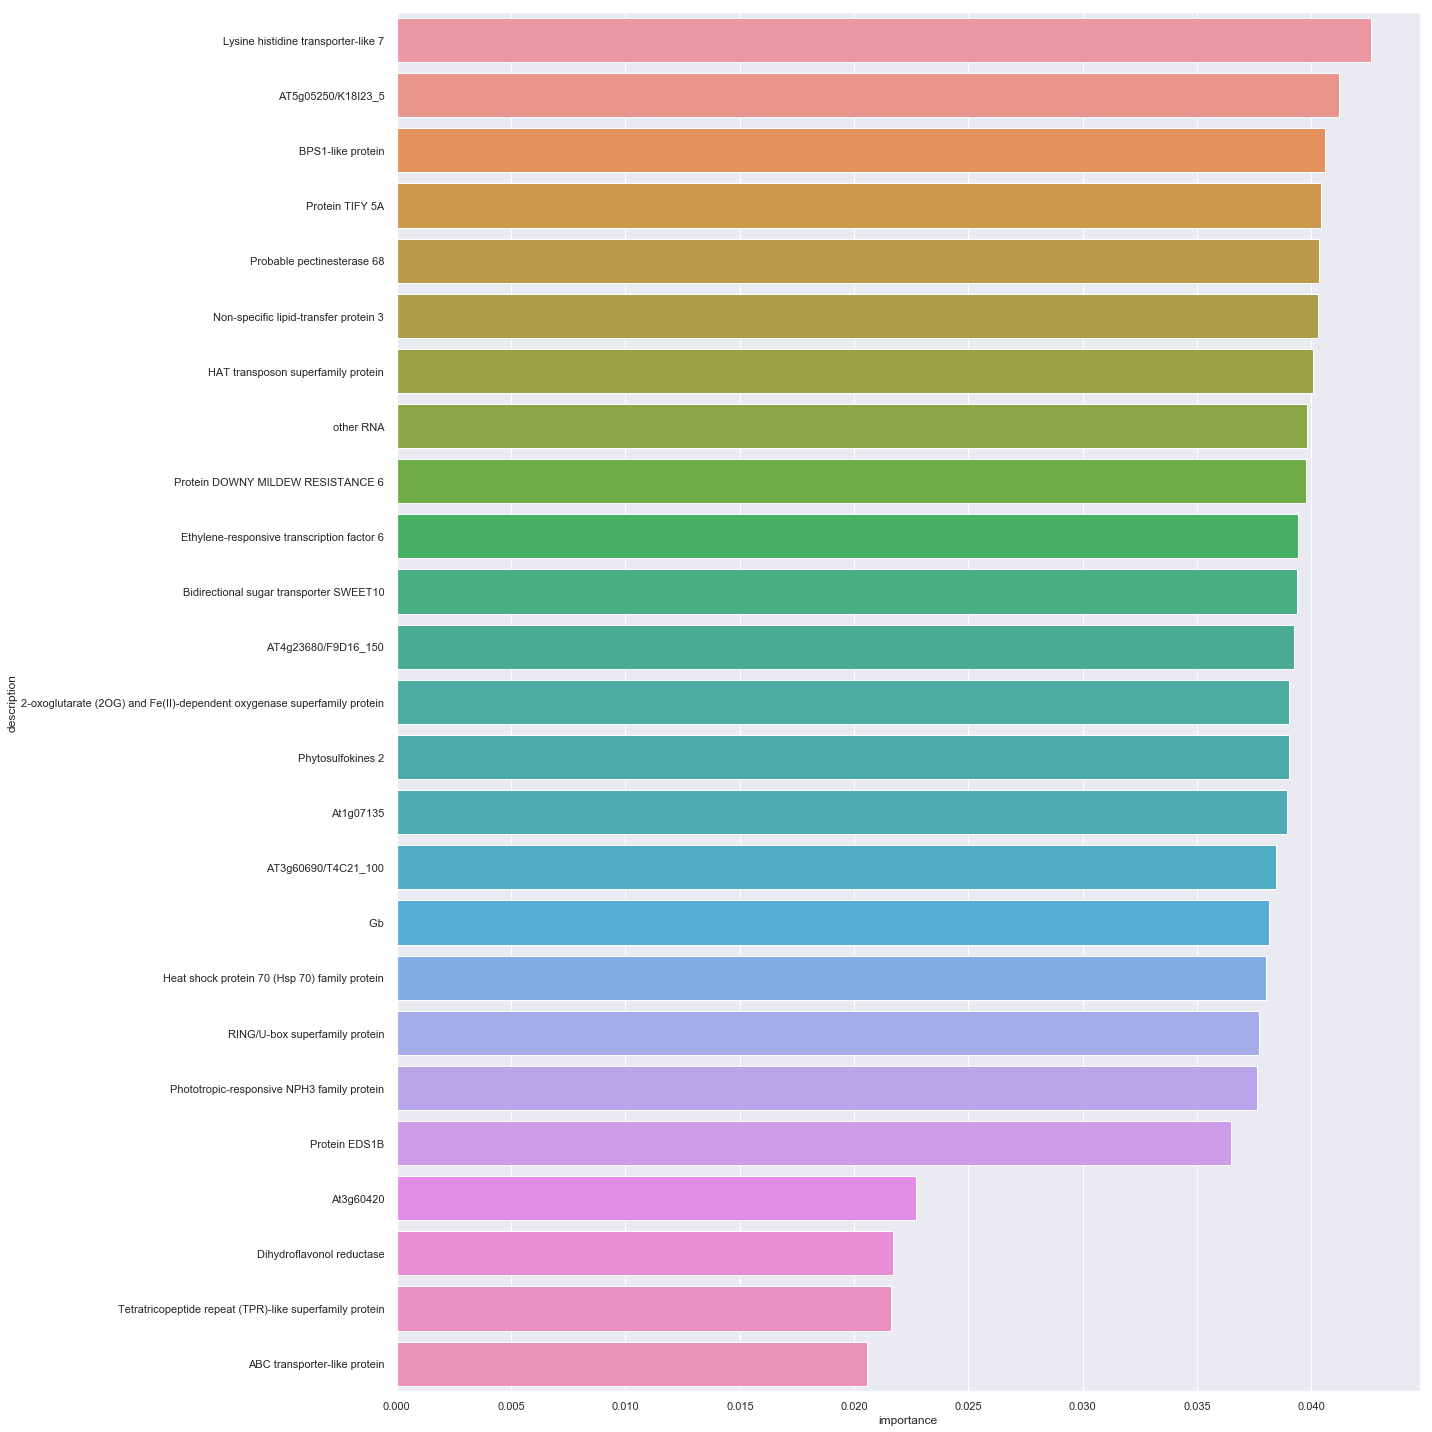
\includegraphics[width=.9\linewidth]{obipy-resources/93e2fbf76ed477962282ae99767b8408de4d3ed9/230825c3322afad31088260ce8154336b50a612e.png}
\end{center}


\subsection{RFE selecting 250 genes}
\label{sec:org8b1489e}
\begin{minted}[frame=lines,linenos=true,fontfamily=Monaco]{ipython}
from sklearn.feature_selection import RFE, RFECV
from sklearn.linear_model import LogisticRegression

# load data
DE_pairings_05hr = read_xl('/Users/hughesn/PHD/Transcripts/Data/pairings_05hr.xlsx')
sig = DE_pairings_05hr[DE_pairings_05hr['padj'] < 0.05]
sig = sig['log2FoldChange'].sort_values()
locs = sig.index
df = counts.loc[locs][[c for c in counts.columns if ('_05h' in c and 'cer' in c)]].T
df = df.loc[:,~df.columns.duplicated()]
df = df[[c for c in set(df.columns.values)]]
\end{minted}

\begin{minted}[frame=lines,linenos=true,fontfamily=Monaco]{ipython}
# Feature Extraction with RFE
X = df.values
y = [y.rsplit('_',1)[0] for y in df.reset_index()['index']]
# feature extraction
model = LogisticRegression()
rfe = RFE(model, n_features_to_select=250)
fit = rfe.fit(X, y)
print("Num Features: {0}".format(fit.n_features_))
print("Selected Features: {0}".format(fit.support_))
print("Feature Ranking: {0}".format(fit.ranking_))
\end{minted}

Num Features: 250\\
Selected Features: [False False False \ldots{} False  True False]\\
Feature Ranking: [4171 1803 1967 \ldots{} 5829    1 3567]\\


\begin{minted}[frame=lines,linenos=true,fontfamily=Monaco]{ipython}
genes = []
for r,f in zip(fit.ranking_, df.columns.values):
      if r ==1:
            genes.append(f)
get_gene_names(genes)
\end{minted}



\begin{center}
\begin{tabular}{rlll}
 & incoming & name & description\\
\hline
0 & AT2G19150 & PME10 & Putative pectinesterase 10\\
1 & AT3G47430 & PEX11B & Peroxisomal membrane protein 11B\\
2 & AT3G01970 & WRKY45 & Probable WRKY transcription factor 45\\
3 & AT3G18915 & AT3G18915 & Transmembrane protein\\
4 & AT3G57910 & AT3G57910 & At3g57910\\
5 & AT3G51330 & AT3G51330 & Eukaryotic aspartyl protease family protein\\
6 & AT5G57760 & AT5G57760 & At5g57760\\
7 & AT2G44700 & AT2G44700 & F-box/kelch-repeat protein At2g44700\\
8 & AT3G30460 & AT3G30460 & RING/U-box superfamily protein\\
9 & AT2G17780 & MCA2 & Protein MID1-COMPLEMENTING ACTIVITY 2\\
10 & AT3G47780 & ABCA7 & ABC transporter A family member 7\\
11 & AT3G52525 & OFP6 & Transcription repressor OFP6\\
12 & AT2G33815 & AT2G33815 & other RNA\\
13 & AT4G01450 & AT4G01450 & WAT1-related protein At4g01450\\
14 & AT1G23830 & AT1G23830 & At1g23830/F5O8\_36\\
15 & AT1G19397 & AT1G19397 & unknown protein\\
16 & AT2G02680 & AT2G02680 & Cysteine/Histidine-rich C1 domain family protein\\
17 & AT1G02390 & GPAT2 & Probable glycerol-3-phosphate acyltransferase 2\\
18 & AT1G18300 & NUDT4 & Nudix hydrolase 4\\
19 & AT2G22890 & FAD4L2 & Fatty acid desaturase 4-like 2, chloroplastic\\
20 & AT4G22467 & AT4G22467 & None\\
21 & AT2G44578 & AT2G44578 & RING/U-box superfamily protein\\
22 & AT4G26790 & AT4G26790 & GDSL esterase/lipase At4g26790\\
23 & AT4G03210 & XTH9 & Xyloglucan endotransglucosylase/hydrolase (Fragment)\\
24 & AT1G17240 & AtRLP2 & receptor like protein 2\\
25 & AT5G49680 & KIP & Protein KINKY POLLEN\\
26 & AT1G48740 & AT1G48740 & 2-oxoglutarate (2OG) and Fe(II)-dependent oxygenase superfamily protein\\
27 & AT5G22794 & AT5G22794 & FUNCTIONS IN: molecular\_function unknown\\
28 & AT5G42800 & DFRA & Dihydroflavonol reductase\\
29 & AT3G13020 & AT3G13020 & HAT transposon superfamily protein\\
30 & AT1G28230 & PUP1 & Purine permease 1\\
31 & AT1G80160 & AT1G80160 & F18B13.24 protein\\
32 & AT1G16830 & AT1G16830 & Putative pentatricopeptide repeat-containing protein At1g16830\\
33 & AT4G11910 & SGR2 & Protein STAY-GREEN 2, chloroplastic\\
34 & AT5G51190 & ERF105 & Ethylene-responsive transcription factor ERF105\\
35 & AT3G15060 & RABA1G & Ras-related protein RABA1g\\
36 & AT5G56030 & HSP81-2 & Heat shock protein 81-2\\
37 & AT4G24570 & PUMP4 & DIC2\\
38 & AT1G79680 & WAKL10 & Wall-associated receptor kinase-like 10\\
39 & AT3G23170 & AT3G23170 & At3g23170\\
40 & AT1G48930 & AtGH9C1 & Endoglucanase 5\\
41 & AT1G29500 & SAUR66 & Auxin-responsive protein SAUR66\\
42 & AT4G02290 & AtGH9B13 & Endoglucanase 17\\
43 & AT3G53270 & AT3G53270 & Small nuclear RNA activating complex (SNAPc), subunit SNAP43 protein\\
44 & AT1G15890 & AT1G15890 & Probable disease resistance protein At1g15890\\
45 & AT3G56790 & AT3G56790 & RNA splicing factor-like protein\\
46 & AT5G26310 & UGT72E3 & Glycosyltransferase (Fragment)\\
47 & AT1G08592 & AT1G08592 & Potential natural antisense gene, locus overlaps with AT1G08590\\
48 & AT1G19025 & AT1G19025 & DNA repair metallo-beta-lactamase family protein\\
49 & AT3G19390 & RD21C & Probable cysteine protease RD21C\\
50 & AT1G49200 & ATL75 & RING-H2 finger protein ATL75\\
51 & AT2G18560 & AT2G18560 & UDP-Glycosyltransferase superfamily protein\\
52 & AT2G04240 & XERICO & Probable E3 ubiquitin-protein ligase XERICO\\
53 & AT2G29460 & GSTU4 & Glutathione S-transferase U4\\
54 & AT4G25220 & RHS15 & Putative glycerol-3-phosphate transporter 2\\
55 & AT3G46320 & AT3G46320 & Histone H4\\
56 & AT1G54970 & PRP1 & Proline-rich protein 1\\
57 & AT1G55365 & AT1G55365 & Putative uncharacterized protein\\
58 & AT4G17500 & ERF1A & Ethylene-responsive transcription factor 1A\\
59 & AT4G26470 & AT4G26470 & Calcium-binding EF-hand family protein\\
60 & AT4G28550 & AT4G28550 & At4g28550\\
61 & AT3G48640 & AT3G48640 & Transmembrane protein\\
62 & AT1G07135 & AT1G07135 & At1g07135\\
63 & AT5G24910 & CYP714A1 & Cytochrome P450 714A1\\
64 & AT2G04050 & DTX3 & Protein DETOXIFICATION 3\\
65 & AT5G21940 & AT5G21940 & At5g21940\\
66 & AT1G75295 & AT1G75295 & other RNA\\
67 & AT1G32920 & AT1G32920 & At1g32920/F9L11\_25\\
68 & AT2G36690 & AT2G36690 & 2-oxoglutarate (2OG) and Fe(II)-dependent oxygenase superfamily protein\\
69 & AT3G63095 & AT3G63095 & Tetratricopeptide repeat (TPR)-like superfamily protein\\
70 & AT3G61760 & DRP1B & DL1B\\
71 & AT4G08985 & AT4G08985 & None\\
72 & AT5G59020 & AT5G59020 & Gb\\
73 & AT1G21100 & IGMT1 & Indole glucosinolate O-methyltransferase 1\\
74 & AT1G35710 & AT1G35710 & Probable leucine-rich repeat receptor-like protein kinase At1g35710\\
75 & AT5G17780 & AT5G17780 & alpha/beta-Hydrolases superfamily protein\\
76 & AT4G01360 & AT4G01360 & BPS1-like protein\\
77 & AT5G02500 & MED37E & Probable mediator of RNA polymerase II transcription subunit 37e\\
78 & AT1G68520 & COL6 & Zinc finger protein CONSTANS-LIKE 6\\
79 & AT4G18197 & PUP7 & Probable purine permease 7\\
80 & AT1G02400 & GA2OX6 & Gibberellin 2-beta-dioxygenase 6\\
81 & AT1G27730 & ZAT10 & Zinc finger protein ZAT10\\
82 & AT3G44260 & CAF1-9 & Probable CCR4-associated factor 1 homolog 9\\
83 & AT2G37430 & ZAT11 & ZAT11\\
84 & AT2G30760 & AT2G30760 & Uncharacterized protein At2g30760\\
85 & AT2G47750 & GH3.9 & Putative indole-3-acetic acid-amido synthetase GH3.9\\
86 & AT5G27420 & ATL31 & E3 ubiquitin-protein ligase ATL31\\
87 & AT3G29000 & CML45 & Probable calcium-binding protein CML45\\
88 & AT4G37100 & AT4G37100 & Pyridoxal phosphate (PLP)-dependent transferases superfamily protein\\
89 & AT2G36650 & AT2G36650 & CHUP1-like protein\\
90 & AT2G41010 & CAMBP25 & Calmodulin-binding protein 25\\
91 & AT1G68450 & VQ8 & VQ motif-containing protein 8, chloroplastic\\
92 & AT1G16510 & SAUR41 & Auxin-responsive protein SAUR41\\
93 & AT5G61600 & ERF104 & Ethylene-responsive transcription factor ERF104\\
94 & AT1G61080 & AT1G61080 & Hydroxyproline-rich glycoprotein family protein\\
95 & AT5G23350 & AT5G23350 & GEM-like protein 6\\
96 & AT4G31805 & POLAR & Protein POLAR LOCALIZATION DURING ASYMMETRIC DIVISION AND REDISTRIBUTION\\
97 & AT5G54860 & AT5G54860 & Probable folate-biopterin transporter 4\\
98 & AT5G35753 & AT5G35753 & Domain of unknown function (DUF3444)\\
99 & AT3G21700 & SGP2 & Monomeric G-protein\\
100 & AT2G18193 & AT2G18193 & AAA-ATPase At2g18193\\
101 & AT4G18880 & HSFA4A & HSF A4A\\
102 & AT2G36800 & UGT73C5 & Glycosyltransferase (Fragment)\\
103 & AT3G43840 & AT3G43840 & 3-oxo-5-alpha-steroid 4-dehydrogenase family protein\\
104 & AT5G05250 & AT5G05250 & AT5g05250/K18I23\_5\\
105 & AT4G21830 & MSRB7 & Peptide methionine sulfoxide reductase B7\\
106 & AT4G23680 & AT4G23680 & AT4g23680/F9D16\_150\\
107 & AT3G16860 & COBL8 & COBRA-like protein 8\\
108 & AT1G76240 & AT1G76240 & At1g76240\\
109 & AT1G32970 & SBT3.2 & Subtilisin-like protease SBT3.2\\
110 & AT5G59220 & SAG113 & Probable protein phosphatase 2C 78\\
111 & AT4G18205 & PUP22 & Probable purine permease 22\\
112 & AT4G16350 & CBL6 & Calcineurin B-like protein 6\\
113 & AT5G59320 & LTP3 & Non-specific lipid-transfer protein 3\\
114 & AT5G62470 & MYB96 & Transcription factor MYB96\\
115 & AT4G24380 & AT4G24380 & INVOLVED IN: 10-formyltetrahydrofolate biosynthetic process, folic acid and derivative biosynthetic process\\
116 & AT3G52780 & PAP20 & Probable purple acid phosphatase 20\\
117 & AT5G43420 & ATL16 & RING-H2 finger protein ATL16\\
118 & AT3G21080 & AT3G21080 & ABC transporter-like protein\\
119 & AT5G64810 & WRKY51 & Probable WRKY transcription factor 51\\
120 & AT5G55840 & AT5G55840 & Pentatricopeptide repeat (PPR) superfamily protein\\
121 & AT1G72300 & PSY1R & Leucine-rich repeat receptor-like protein kinase (Fragment)\\
122 & AT4G15270 & AT4G15270 & Glucosyltransferase-like protein (Fragment)\\
123 & AT4G31510 & AT4G31510 & Major centromere autoantigen B-like protein\\
124 & AT5G52545 & AT5G52545 & unknown protein\\
125 & AT4G21865 & AT4G21865 & At4g21865\\
126 & AT5G05300 & AT5G05300 & Gb\\
127 & AT5G20710 & BGAL7 & Beta-galactosidase 7\\
128 & AT1G24260 & SEP3 & At1g24260\\
129 & AT5G66080 & AT5G66080 & Probable protein phosphatase 2C 79\\
130 & AT2G45760 & BAP2 & BON1-associated protein 2\\
131 & AT1G11050 & AT1G11050 & Probable receptor-like protein kinase At1g11050\\
132 & AT4G35730 & AT4G35730 & Regulator of Vps4 activity in the MVB pathway protein\\
133 & AT2G32030 & AT2G32030 & Acyl-CoA N-acyltransferases (NAT) superfamily protein\\
134 & AT5G57560 & XTH22 & Xyloglucan endotransglucosylase/hydrolase\\
135 & AT4G22710 & CYP706A2 & Cytochrome P450 - like protein\\
136 & AT4G05910 & AT4G05910 & None\\
137 & AT1G30135 & TIFY5A & Protein TIFY 5A\\
138 & AT3G54590 & EXT2 & Extensin-2\\
139 & AT5G56010 & HSP90-3 & Heat shock protein 90-3\\
140 & AT5G19070 & AT5G19070 & At5g19070\\
141 & AT5G57770 & AT5G57770 & Plant protein of unknown function (DUF828) with plant pleckstrin homology-like region\\
142 & AT3G03000 & CML18 & Probable calcium-binding protein CML18\\
143 & AT5G21960 & ERF016 & Ethylene-responsive transcription factor ERF016\\
144 & AT5G41080 & GDPD2 & Glycerophosphodiester phosphodiesterase GDPD2\\
145 & AT1G69790 & PBL18 & Probable serine/threonine-protein kinase PBL18\\
146 & AT2G18210 & AT2G18210 & At2g18210\\
147 & AT4G11280 & ACS6 & 1-aminocyclopropane-1-carboxylate synthase 6\\
148 & AT3G02210 & COBL1 & COBRA-like protein\\
149 & AT5G17220 & GSTF12 & Glutathione S-transferase F12\\
150 & AT1G31290 & AGO3 & Protein argonaute 3\\
151 & AT5G25280 & AT5G25280 & AT5g25280/F18G18\_20\\
152 & AT1G55430 & AT1G55430 & Cysteine/Histidine-rich C1 domain family protein\\
153 & AT5G19080 & LUL3 & Probable E3 ubiquitin-protein ligase LUL3\\
154 & AT1G69910 & LRK10L-1.5 & LEAF RUST 10 DISEASE-RESISTANCE LOCUS RECEPTOR-LIKE PROTEIN KINASE-like 1.5\\
155 & AT1G78090 & TPPB & Trehalose-phosphate phosphatase B\\
156 & AT5G40780 & LHT1 & Lysine histidine transporter 1\\
157 & AT3G61800 & AT3G61800 & UV-stimulated scaffold protein A homolog\\
158 & AT1G72520 & LOX4 & Lipoxygenase 4, chloroplastic\\
159 & AT4G08935 & AT4G08935 & None\\
160 & AT1G66500 & PCFS1 & Polyadenylation and cleavage factor homolog 1\\
161 & AT3G43580 & AT3G43580 & At3g43580\\
162 & AT1G19020 & AT1G19020 & CDP-diacylglycerol-glycerol-3-phosphate 3-phosphatidyltransferase\\
163 & AT1G76650 & CML38 & CML38\\
164 & AT1G77000 & SKP2B & F-box protein SKP2B\\
165 & AT1G56242 & AT1G56242 & other RNA\\
166 & AT5G23990 & ATFRO5 & ferric reduction oxidase 5\\
167 & AT5G22250 & CAF1-11 & Probable CCR4-associated factor 1 homolog 11\\
168 & AT2G16870 & AT2G16870 & Disease resistance protein (TIR-NBS-LRR class) family\\
169 & AT3G49620 & DIN11 & Probable 2-oxoglutarate-dependent dioxygenase DIN11\\
170 & AT3G55090 & ABCG16 & ABC transporter G family member 16\\
171 & AT3G60415 & AT3G60415 & At3g60420\\
172 & AT1G33170 & AT1G33170 & Probable methyltransferase PMT18\\
173 & AT5G51720 & NEET & NEET\\
174 & AT1G48500 & TIFY6A & Protein TIFY 6A\\
175 & AT3G57630 & AT3G57630 & At3g57630\\
176 & AT2G35980 & NHL10 & NDR1/HIN1-like protein 10\\
177 & AT1G73740 & AT1G73740 & Putative UDP-N-acetylglucosamine--N-acetylmuramyl-(Pentapeptide)-pyrophosphoryl-undecaprenol N-acetylglucosamine transferase\\
178 & AT3G09440 & HSP70-3 & Heat shock protein 70 (Hsp 70) family protein\\
179 & AT1G24148 & AT1G24148 & unknown protein\\
180 & AT1G27370 & SPL10 & Squamosa promoter-binding-like protein 10\\
181 & AT3G50770 & CML41 & Probable calcium-binding protein CML41\\
182 & AT1G02405 & AT1G02405 & At1g02405\\
183 & AT1G05950 & AT1G05950 & unknown protein\\
184 & AT2G01900 & AT2G01900 & DNAse I-like superfamily protein\\
185 & AT5G06839 & TGA10 & Transcription factor TGA10\\
186 & AT2G21210 & AT2G21210 & SAUR-like auxin-responsive protein family\\
187 & AT1G63580 & CRRSP6 & Probable cysteine-rich repeat secretory protein 6\\
188 & AT5G51465 & AT5G51465 & None\\
189 & AT2G39370 & MAKR4 & Probable membrane-associated kinase regulator 4\\
190 & AT5G56220 & AT5G56220 & P-loop containing nucleoside triphosphate hydrolases superfamily protein\\
191 & AT3G56880 & AT3G56880 & VQ motif-containing protein\\
192 & AT2G09975 & AT2G09975 & None\\
193 & AT5G53450 & PAP14 & Probable plastid-lipid-associated protein 14, chloroplastic\\
194 & AT1G17420 & LOX3 & Lipoxygenase 3, chloroplastic\\
195 & AT3G14475 & AT3G14475 & snoRNA\\
196 & AT2G36430 & AT2G36430 & Transmembrane protein, putative (DUF247)\\
197 & AT4G31330 & AT4G31330 & Uncharacterized protein At4g31330\\
198 & AT4G29180 & RHS16 & RHS16\\
199 & AT5G56750 & NDL1 & Protein NDL1\\
200 & AT3G07900 & OFUT24 & O-fucosyltransferase 24\\
201 & AT5G66000 & AT5G66000 & Uncharacterized protein At5g66000\\
202 & AT1G60080 & AT1G60080 & 3'-5'-exoribonuclease family protein\\
203 & AT4G31550 & WRKY11 & Probable WRKY transcription factor 11\\
204 & AT1G80640 & AT1G80640 & Probable receptor-like protein kinase At1g80640\\
205 & AT5G50790 & SWEET10 & Bidirectional sugar transporter SWEET10\\
206 & AT3G60550 & CYCU2-2 & Cyclin-U2-2\\
207 & AT2G22860 & PSK2 & Phytosulfokines 2\\
208 & AT2G15390 & FUT4 & Probable fucosyltransferase 4\\
209 & AT1G60590 & AT1G60590 & Pectin lyase-like superfamily protein\\
210 & AT1G69930 & GSTU11 & Glutathione S-transferase U11\\
211 & AT3G60690 & AT3G60690 & AT3g60690/T4C21\_100\\
212 & AT2G45870 & AT2G45870 & UPF0187 protein At2g45870, chloroplastic\\
213 & AT1G07143 & AT1G07143 & None\\
214 & AT2G32150 & AT2G32150 & At2g32150/F22D22.10\\
215 & AT5G60310 & LECRK110 & Putative L-type lectin-domain containing receptor kinase I.10\\
216 & AT1G63350 & AT1G63350 & Disease resistance protein (CC-NBS-LRR class) family\\
217 & AT4G17490 & ERF6 & Ethylene-responsive transcription factor 6\\
218 & AT3G48080 & EDS1B & Protein EDS1B\\
219 & AT1G69890 & AT1G69890 & Actin cross-linking protein (DUF569)\\
220 & AT4G35180 & LHT7 & Lysine histidine transporter-like 7\\
221 & AT1G61840 & AT1G61840 & Cysteine/Histidine-rich C1 domain family protein\\
222 & AT2G02635 & AT2G02635 & None\\
223 & AT1G21120 & AT1G21120 & O-methyltransferase family protein\\
224 & AT5G08070 & TCP17 & Transcription factor TCP17\\
225 & AT4G35770 & STR15 & SEN1\\
226 & AT4G15070 & AT4G15070 & Cysteine/Histidine-rich C1 domain family protein\\
227 & AT5G57625 & AT5G57625 & At5g57625\\
228 & AT3G49900 & AT3G49900 & Phototropic-responsive NPH3 family protein\\
229 & AT5G24210 & AT5G24210 & Alpha/beta-Hydrolases superfamily protein\\
230 & AT3G55980 & SZF1 & Salt-inducible zinc finger 1\\
231 & AT5G47500 & PME68 & Probable pectinesterase 68\\
232 & AT4G27657 & AT4G27657 & At4g27657\\
233 & AT3G61280 & AT3G61280 & Glycosyltransferase\\
234 & AT4G38950 & KIN7F & Kinesin-like protein KIN-7F\\
235 & AT1G21110 & IGMT3 & Indole glucosinolate O-methyltransferase 3\\
236 & AT5G36970 & NHL25 & NHL25\\
237 & AT5G46350 & WRKY8 & WRKY transcription factor 8\\
238 & AT2G26530 & AR781 & AR781\\
239 & AT2G35000 & ATL9 & E3 ubiquitin-protein ligase ATL9\\
240 & AT4G19230 & CYP707A1 & Cytochrome P450, family 707, subfamily A, polypeptide 1\\
241 & AT3G22830 & HSFA6B & Heat stress transcription factor A-6b\\
242 & AT4G04540 & CRK39 & Putative cysteine-rich receptor-like protein kinase 39\\
243 & AT4G24110 & AT4G24110 & NADP-specific glutamate dehydrogenase\\
244 & AT5G24530 & DMR6 & Protein DOWNY MILDEW RESISTANCE 6\\
245 & AT1G54650 & AT1G54650 & Methyltransferase family protein\\
246 & AT3G05600 & AT3G05600 & Alpha/beta-Hydrolases superfamily protein\\
247 & AT1G51660 & MKK4 & MKK4\\
248 & AT2G47190 & ATMYB2 & ATMYB2\\
249 & AT3G52400 & SYP122 & Syntaxin-122\\
\end{tabular}
\end{center}


\paragraph{Forest on this RFE set}
\label{sec:orgf977315}

\begin{minted}[frame=lines,linenos=true,fontfamily=Monaco]{ipython}
rfe_forest = counts.loc[genes][[c for c in counts.columns if ('_05h' in c and 'cer' in c)]].T
rfe_forest = rfe_forest.loc[:,~rfe_forest.columns.duplicated()]
rfe_forest = rfe_forest[[c for c in set(rfe_forest.columns.values)]]

feat_labels = rfe_forest.columns.values
y = [d.rsplit('_', 1)[0] for d in rfe_forest.index.values]

X_train, X_test, y_train, y_test = train_test_split(rfe_forest.values, y, test_size=1, random_state=42)
forest = RandomForestClassifier(n_estimators=20000, random_state=1, n_jobs=-1)
forest.fit(X_train, y_train)
res = {k: v for k, v in sorted(
    zip(feat_labels, forest.feature_importances_), key=lambda x: x[1], reverse=True)}
res_df = pd.DataFrame(list(res.items()), columns=[
                      'gene', 'importance']).set_index('gene')
names = get_gene_names(list(res_df.index))
res_df = pd.merge(res_df, names, left_index=True, right_on='incoming').rename(
    columns={'incoming': 'gene'}).set_index('gene').sort_values('importance', ascending=False)
res_df
\end{minted}

\begin{center}
\begin{tabular}{lrll}
gene & importance & name & description\\
\hline
AT3G61280 & 0.0055 & AT3G61280 & Glycosyltransferase\\
AT4G15070 & 0.0054 & AT4G15070 & Cysteine/Histidine-rich C1 domain family protein\\
AT1G60590 & 0.0053 & AT1G60590 & Pectin lyase-like superfamily protein\\
AT1G17420 & 0.0052 & LOX3 & Lipoxygenase 3, chloroplastic\\
AT5G59020 & 0.0052 & AT5G59020 & Gb\\
AT1G02390 & 0.00515 & GPAT2 & Probable glycerol-3-phosphate acyltransferase 2\\
AT1G18300 & 0.00505 & NUDT4 & Nudix hydrolase 4\\
AT5G51720 & 0.005 & NEET & NEET\\
AT3G52400 & 0.005 & SYP122 & Syntaxin-122\\
AT5G22250 & 0.00495 & CAF1-11 & Probable CCR4-associated factor 1 homolog 11\\
AT4G01360 & 0.00495 & AT4G01360 & BPS1-like protein\\
AT4G02290 & 0.00495 & AtGH9B13 & Endoglucanase 17\\
AT3G05600 & 0.00495 & AT3G05600 & Alpha/beta-Hydrolases superfamily protein\\
AT3G55090 & 0.0049 & ABCG16 & ABC transporter G family member 16\\
AT4G29180 & 0.00485 & RHS16 & RHS16\\
AT4G08935 & 0.00485 & AT4G08935 & None\\
AT4G18197 & 0.0048 & PUP7 & Probable purine permease 7\\
AT3G18915 & 0.0048 & AT3G18915 & Transmembrane protein\\
AT4G24110 & 0.0048 & AT4G24110 & NADP-specific glutamate dehydrogenase\\
AT5G08070 & 0.0048 & TCP17 & Transcription factor TCP17\\
AT4G22710 & 0.0048 & CYP706A2 & Cytochrome P450 - like protein\\
AT4G05910 & 0.0048 & AT4G05910 & None\\
AT5G22794 & 0.0048 & AT5G22794 & FUNCTIONS IN: molecular\_function unknown\\
AT3G47430 & 0.0048 & PEX11B & Peroxisomal membrane protein 11B\\
AT2G04240 & 0.0048 & XERICO & Probable E3 ubiquitin-protein ligase XERICO\\
AT3G61800 & 0.00475 & AT3G61800 & UV-stimulated scaffold protein A homolog\\
AT3G29000 & 0.00475 & CML45 & Probable calcium-binding protein CML45\\
AT5G57760 & 0.00475 & AT5G57760 & At5g57760\\
AT2G32030 & 0.0047 & AT2G32030 & Acyl-CoA N-acyltransferases (NAT) superfamily protein\\
AT2G36800 & 0.0047 & UGT73C5 & Glycosyltransferase (Fragment)\\
AT5G02500 & 0.0047 & MED37E & Probable mediator of RNA polymerase II transcription subunit 37e\\
AT2G16870 & 0.0047 & AT2G16870 & Disease resistance protein (TIR-NBS-LRR class) family\\
AT2G36650 & 0.0047 & AT2G36650 & CHUP1-like protein\\
AT4G01450 & 0.00465 & AT4G01450 & WAT1-related protein At4g01450\\
AT1G69890 & 0.00465 & AT1G69890 & Actin cross-linking protein (DUF569)\\
AT4G31510 & 0.00465 & AT4G31510 & Major centromere autoantigen B-like protein\\
AT1G32970 & 0.00465 & SBT3.2 & Subtilisin-like protease SBT3.2\\
AT3G03000 & 0.00465 & CML18 & Probable calcium-binding protein CML18\\
AT5G55840 & 0.00465 & AT5G55840 & Pentatricopeptide repeat (PPR) superfamily protein\\
AT4G19230 & 0.00465 & CYP707A1 & Cytochrome P450, family 707, subfamily A, polypeptide 1\\
AT1G07135 & 0.00465 & AT1G07135 & At1g07135\\
AT2G45870 & 0.0046 & AT2G45870 & UPF0187 protein At2g45870, chloroplastic\\
AT5G59320 & 0.0046 & LTP3 & Non-specific lipid-transfer protein 3\\
AT2G22890 & 0.0046 & FAD4L2 & Fatty acid desaturase 4-like 2, chloroplastic\\
AT2G02680 & 0.0046 & AT2G02680 & Cysteine/Histidine-rich C1 domain family protein\\
AT5G57560 & 0.0046 & XTH22 & Xyloglucan endotransglucosylase/hydrolase\\
AT4G03210 & 0.00455 & XTH9 & Xyloglucan endotransglucosylase/hydrolase (Fragment)\\
AT3G56880 & 0.00455 & AT3G56880 & VQ motif-containing protein\\
AT5G24530 & 0.00455 & DMR6 & Protein DOWNY MILDEW RESISTANCE 6\\
AT5G62470 & 0.00455 & MYB96 & Transcription factor MYB96\\
AT5G47500 & 0.00455 & PME68 & Probable pectinesterase 68\\
AT1G49200 & 0.00455 & ATL75 & RING-H2 finger protein ATL75\\
AT5G52545 & 0.00455 & AT5G52545 & unknown protein\\
AT5G59220 & 0.00455 & SAG113 & Probable protein phosphatase 2C 78\\
AT2G01900 & 0.0045 & AT2G01900 & DNAse I-like superfamily protein\\
AT4G35730 & 0.0045 & AT4G35730 & Regulator of Vps4 activity in the MVB pathway protein\\
AT2G22860 & 0.0045 & PSK2 & Phytosulfokines 2\\
AT4G31550 & 0.0045 & WRKY11 & Probable WRKY transcription factor 11\\
AT5G56220 & 0.0045 & AT5G56220 & P-loop containing nucleoside triphosphate hydrolases superfamily protein\\
AT1G80640 & 0.0045 & AT1G80640 & Probable receptor-like protein kinase At1g80640\\
AT4G18880 & 0.00445 & HSFA4A & HSF A4A\\
AT3G61760 & 0.00445 & DRP1B & DL1B\\
AT1G75295 & 0.00445 & AT1G75295 & other RNA\\
AT5G40780 & 0.00445 & LHT1 & Lysine histidine transporter 1\\
AT1G21120 & 0.00445 & AT1G21120 & O-methyltransferase family protein\\
AT3G56790 & 0.0044 & AT3G56790 & RNA splicing factor-like protein\\
AT1G33170 & 0.0044 & AT1G33170 & Probable methyltransferase PMT18\\
AT3G51330 & 0.0044 & AT3G51330 & Eukaryotic aspartyl protease family protein\\
AT5G61600 & 0.0044 & ERF104 & Ethylene-responsive transcription factor ERF104\\
AT2G18560 & 0.0044 & AT2G18560 & UDP-Glycosyltransferase superfamily protein\\
AT2G36430 & 0.00435 & AT2G36430 & Transmembrane protein, putative (DUF247)\\
AT4G25220 & 0.00435 & RHS15 & Putative glycerol-3-phosphate transporter 2\\
AT1G15890 & 0.00435 & AT1G15890 & Probable disease resistance protein At1g15890\\
AT3G44260 & 0.00435 & CAF1-9 & Probable CCR4-associated factor 1 homolog 9\\
AT1G68520 & 0.00435 & COL6 & Zinc finger protein CONSTANS-LIKE 6\\
AT2G44700 & 0.00435 & AT2G44700 & F-box/kelch-repeat protein At2g44700\\
AT3G49900 & 0.00435 & AT3G49900 & Phototropic-responsive NPH3 family protein\\
AT5G49680 & 0.00435 & KIP & Protein KINKY POLLEN\\
AT1G02400 & 0.00435 & GA2OX6 & Gibberellin 2-beta-dioxygenase 6\\
AT1G02405 & 0.00435 & AT1G02405 & At1g02405\\
AT2G18210 & 0.00435 & AT2G18210 & At2g18210\\
AT1G55365 & 0.0043 & AT1G55365 & Putative uncharacterized protein\\
AT5G25280 & 0.0043 & AT5G25280 & AT5g25280/F18G18\_20\\
AT1G69930 & 0.0043 & GSTU11 & Glutathione S-transferase U11\\
AT4G31805 & 0.0043 & POLAR & Protein POLAR LOCALIZATION DURING ASYMMETRIC DIVISION AND REDISTRIBUTION\\
AT3G13020 & 0.0043 & AT3G13020 & HAT transposon superfamily protein\\
AT5G23350 & 0.0043 & AT5G23350 & GEM-like protein 6\\
AT2G35980 & 0.0043 & NHL10 & NDR1/HIN1-like protein 10\\
AT2G17780 & 0.0043 & MCA2 & Protein MID1-COMPLEMENTING ACTIVITY 2\\
AT3G60690 & 0.0043 & AT3G60690 & AT3g60690/T4C21\_100\\
AT2G18193 & 0.00425 & AT2G18193 & AAA-ATPase At2g18193\\
AT5G20710 & 0.00425 & BGAL7 & Beta-galactosidase 7\\
AT1G56242 & 0.00425 & AT1G56242 & other RNA\\
AT4G15270 & 0.00425 & AT4G15270 & Glucosyltransferase-like protein (Fragment)\\
AT4G38950 & 0.00425 & KIN7F & Kinesin-like protein KIN-7F\\
AT4G27657 & 0.00425 & AT4G27657 & At4g27657\\
AT5G35753 & 0.00425 & AT5G35753 & Domain of unknown function (DUF3444)\\
AT1G17240 & 0.00425 & AtRLP2 & receptor like protein 2\\
AT1G19025 & 0.0042 & AT1G19025 & DNA repair metallo-beta-lactamase family protein\\
AT1G61080 & 0.0042 & AT1G61080 & Hydroxyproline-rich glycoprotein family protein\\
AT4G23680 & 0.0042 & AT4G23680 & AT4g23680/F9D16\_150\\
AT1G77000 & 0.0042 & SKP2B & F-box protein SKP2B\\
AT5G56030 & 0.0042 & HSP81-2 & Heat shock protein 81-2\\
AT4G16350 & 0.0042 & CBL6 & Calcineurin B-like protein 6\\
AT1G60080 & 0.0042 & AT1G60080 & 3'-5'-exoribonuclease family protein\\
AT2G47190 & 0.00415 & ATMYB2 & ATMYB2\\
AT1G48500 & 0.00415 & TIFY6A & Protein TIFY 6A\\
AT2G29460 & 0.00415 & GSTU4 & Glutathione S-transferase U4\\
AT3G48080 & 0.00415 & EDS1B & Protein EDS1B\\
AT1G27370 & 0.00415 & SPL10 & Squamosa promoter-binding-like protein 10\\
AT4G26470 & 0.00415 & AT4G26470 & Calcium-binding EF-hand family protein\\
AT5G50790 & 0.0041 & SWEET10 & Bidirectional sugar transporter SWEET10\\
AT1G19020 & 0.0041 & AT1G19020 & CDP-diacylglycerol-glycerol-3-phosphate 3-phosphatidyltransferase\\
AT2G35000 & 0.0041 & ATL9 & E3 ubiquitin-protein ligase ATL9\\
AT4G26790 & 0.0041 & AT4G26790 & GDSL esterase/lipase At4g26790\\
AT5G51190 & 0.0041 & ERF105 & Ethylene-responsive transcription factor ERF105\\
AT4G17500 & 0.0041 & ERF1A & Ethylene-responsive transcription factor 1A\\
AT4G24380 & 0.0041 & AT4G24380 & INVOLVED IN: 10-formyltetrahydrofolate biosynthetic process, folic acid and derivative biosynthetic process\\
AT1G66500 & 0.00405 & PCFS1 & Polyadenylation and cleavage factor homolog 1\\
AT2G02635 & 0.00405 & AT2G02635 & None\\
AT1G54970 & 0.00405 & PRP1 & Proline-rich protein 1\\
AT5G21960 & 0.00405 & ERF016 & Ethylene-responsive transcription factor ERF016\\
AT3G23170 & 0.00405 & AT3G23170 & At3g23170\\
AT1G29500 & 0.00405 & SAUR66 & Auxin-responsive protein SAUR66\\
AT5G46350 & 0.00405 & WRKY8 & WRKY transcription factor 8\\
AT2G44578 & 0.00405 & AT2G44578 & RING/U-box superfamily protein\\
AT1G32920 & 0.00405 & AT1G32920 & At1g32920/F9L11\_25\\
AT4G21865 & 0.00405 & AT4G21865 & At4g21865\\
AT5G05250 & 0.004 & AT5G05250 & AT5g05250/K18I23\_5\\
AT1G24260 & 0.004 & SEP3 & At1g24260\\
AT1G30135 & 0.004 & TIFY5A & Protein TIFY 5A\\
AT2G47750 & 0.004 & GH3.9 & Putative indole-3-acetic acid-amido synthetase GH3.9\\
AT4G31330 & 0.004 & AT4G31330 & Uncharacterized protein At4g31330\\
AT2G21210 & 0.004 & AT2G21210 & SAUR-like auxin-responsive protein family\\
AT3G01970 & 0.00395 & WRKY45 & Probable WRKY transcription factor 45\\
AT5G21940 & 0.00395 & AT5G21940 & At5g21940\\
AT1G79680 & 0.00395 & WAKL10 & Wall-associated receptor kinase-like 10\\
AT5G05300 & 0.00395 & AT5G05300 & Gb\\
AT5G17780 & 0.00395 & AT5G17780 & alpha/beta-Hydrolases superfamily protein\\
AT3G14475 & 0.00395 & AT3G14475 & snoRNA\\
AT4G21830 & 0.00395 & MSRB7 & Peptide methionine sulfoxide reductase B7\\
AT1G31290 & 0.00395 & AGO3 & Protein argonaute 3\\
AT3G46320 & 0.0039 & AT3G46320 & Histone H4\\
AT5G19080 & 0.0039 & LUL3 & Probable E3 ubiquitin-protein ligase LUL3\\
AT3G21700 & 0.0039 & SGP2 & Monomeric G-protein\\
AT1G07143 & 0.0039 & AT1G07143 & None\\
AT1G16510 & 0.0039 & SAUR41 & Auxin-responsive protein SAUR41\\
AT5G56010 & 0.0039 & HSP90-3 & Heat shock protein 90-3\\
AT4G17490 & 0.00385 & ERF6 & Ethylene-responsive transcription factor 6\\
AT3G54590 & 0.00385 & EXT2 & Extensin-2\\
AT2G37430 & 0.00385 & ZAT11 & ZAT11\\
AT3G09440 & 0.0038 & HSP70-3 & Heat shock protein 70 (Hsp 70) family protein\\
AT4G11910 & 0.0038 & SGR2 & Protein STAY-GREEN 2, chloroplastic\\
AT1G76650 & 0.0038 & CML38 & CML38\\
AT5G26310 & 0.0038 & UGT72E3 & Glycosyltransferase (Fragment)\\
AT5G27420 & 0.0038 & ATL31 & E3 ubiquitin-protein ligase ATL31\\
AT5G19070 & 0.0038 & AT5G19070 & At5g19070\\
AT1G11050 & 0.00375 & AT1G11050 & Probable receptor-like protein kinase At1g11050\\
AT5G56750 & 0.00375 & NDL1 & Protein NDL1\\
AT3G60550 & 0.00375 & CYCU2-2 & Cyclin-U2-2\\
AT5G06839 & 0.00375 & TGA10 & Transcription factor TGA10\\
AT3G19390 & 0.00375 & RD21C & Probable cysteine protease RD21C\\
AT1G28230 & 0.00375 & PUP1 & Purine permease 1\\
AT3G22830 & 0.00375 & HSFA6B & Heat stress transcription factor A-6b\\
AT1G55430 & 0.0037 & AT1G55430 & Cysteine/Histidine-rich C1 domain family protein\\
AT1G54650 & 0.0037 & AT1G54650 & Methyltransferase family protein\\
AT5G57770 & 0.00365 & AT5G57770 & Plant protein of unknown function (DUF828) with plant pleckstrin homology-like region\\
AT4G35180 & 0.00365 & LHT7 & Lysine histidine transporter-like 7\\
AT5G66000 & 0.0036 & AT5G66000 & Uncharacterized protein At5g66000\\
AT1G16830 & 0.0036 & AT1G16830 & Putative pentatricopeptide repeat-containing protein At1g16830\\
AT1G05950 & 0.0036 & AT1G05950 & unknown protein\\
AT4G37100 & 0.00355 & AT4G37100 & Pyridoxal phosphate (PLP)-dependent transferases superfamily protein\\
AT2G32150 & 0.0035 & AT2G32150 & At2g32150/F22D22.10\\
AT4G18205 & 0.00345 & PUP22 & Probable purine permease 22\\
AT5G41080 & 0.00345 & GDPD2 & Glycerophosphodiester phosphodiesterase GDPD2\\
AT2G41010 & 0.0034 & CAMBP25 & Calmodulin-binding protein 25\\
AT4G28550 & 0.0034 & AT4G28550 & At4g28550\\
AT2G45760 & 0.0034 & BAP2 & BON1-associated protein 2\\
AT1G48740 & 0.0033 & AT1G48740 & 2-oxoglutarate (2OG) and Fe(II)-dependent oxygenase superfamily protein\\
AT2G39370 & 0.0032 & MAKR4 & Probable membrane-associated kinase regulator 4\\
AT5G42800 & 0.0031 & DFRA & Dihydroflavonol reductase\\
AT4G11280 & 0.0031 & ACS6 & 1-aminocyclopropane-1-carboxylate synthase 6\\
AT3G53270 & 0.0031 & AT3G53270 & Small nuclear RNA activating complex (SNAPc), subunit SNAP43 protein\\
AT3G57630 & 0.00285 & AT3G57630 & At3g57630\\
AT2G15390 & 0.00275 & FUT4 & Probable fucosyltransferase 4\\
AT2G04050 & 0.00275 & DTX3 & Protein DETOXIFICATION 3\\
AT4G24570 & 0.00275 & PUMP4 & DIC2\\
AT3G21080 & 0.00275 & AT3G21080 & ABC transporter-like protein\\
AT1G24148 & 0.00275 & AT1G24148 & unknown protein\\
AT1G23830 & 0.00265 & AT1G23830 & At1g23830/F5O8\_36\\
AT2G30760 & 0.00265 & AT2G30760 & Uncharacterized protein At2g30760\\
AT3G57910 & 0.0026 & AT3G57910 & At3g57910\\
AT2G26530 & 0.0026 & AR781 & AR781\\
AT3G43580 & 0.00255 & AT3G43580 & At3g43580\\
AT4G04540 & 0.0025 & CRK39 & Putative cysteine-rich receptor-like protein kinase 39\\
AT1G69910 & 0.00245 & LRK10L-1.5 & LEAF RUST 10 DISEASE-RESISTANCE LOCUS RECEPTOR-LIKE PROTEIN KINASE-like 1.5\\
AT1G63350 & 0.0024 & AT1G63350 & Disease resistance protein (CC-NBS-LRR class) family\\
AT3G60415 & 0.0024 & AT3G60415 & At3g60420\\
AT2G09975 & 0.0024 & AT2G09975 & None\\
AT3G16860 & 0.0024 & COBL8 & COBRA-like protein 8\\
AT3G43840 & 0.00235 & AT3G43840 & 3-oxo-5-alpha-steroid 4-dehydrogenase family protein\\
AT5G24210 & 0.0023 & AT5G24210 & Alpha/beta-Hydrolases superfamily protein\\
AT1G08592 & 0.0023 & AT1G08592 & Potential natural antisense gene, locus overlaps with AT1G08590\\
AT3G48640 & 0.0023 & AT3G48640 & Transmembrane protein\\
AT1G27730 & 0.00225 & ZAT10 & Zinc finger protein ZAT10\\
AT5G66080 & 0.00225 & AT5G66080 & Probable protein phosphatase 2C 79\\
AT3G63095 & 0.00225 & AT3G63095 & Tetratricopeptide repeat (TPR)-like superfamily protein\\
AT5G43420 & 0.0022 & ATL16 & RING-H2 finger protein ATL16\\
AT5G64810 & 0.00215 & WRKY51 & Probable WRKY transcription factor 51\\
AT1G72300 & 0.00215 & PSY1R & Leucine-rich repeat receptor-like protein kinase (Fragment)\\
AT3G02210 & 0.00215 & COBL1 & COBRA-like protein\\
AT3G07900 & 0.0021 & OFUT24 & O-fucosyltransferase 24\\
AT5G54860 & 0.0021 & AT5G54860 & Probable folate-biopterin transporter 4\\
AT1G19397 & 0.0021 & AT1G19397 & unknown protein\\
AT5G53450 & 0.00205 & PAP14 & Probable plastid-lipid-associated protein 14, chloroplastic\\
AT2G19150 & 0.00205 & PME10 & Putative pectinesterase 10\\
AT1G80160 & 0.002 & AT1G80160 & F18B13.24 protein\\
AT5G17220 & 0.002 & GSTF12 & Glutathione S-transferase F12\\
AT4G08985 & 0.002 & AT4G08985 & None\\
AT3G30460 & 0.00195 & AT3G30460 & RING/U-box superfamily protein\\
AT1G21100 & 0.0019 & IGMT1 & Indole glucosinolate O-methyltransferase 1\\
AT1G72520 & 0.0019 & LOX4 & Lipoxygenase 4, chloroplastic\\
AT4G35770 & 0.0019 & STR15 & SEN1\\
AT2G36690 & 0.0019 & AT2G36690 & 2-oxoglutarate (2OG) and Fe(II)-dependent oxygenase superfamily protein\\
AT1G61840 & 0.0019 & AT1G61840 & Cysteine/Histidine-rich C1 domain family protein\\
AT5G23990 & 0.00185 & ATFRO5 & ferric reduction oxidase 5\\
AT1G35710 & 0.0018 & AT1G35710 & Probable leucine-rich repeat receptor-like protein kinase At1g35710\\
AT3G55980 & 0.0018 & SZF1 & Salt-inducible zinc finger 1\\
AT3G52525 & 0.00175 & OFP6 & Transcription repressor OFP6\\
AT5G24910 & 0.00175 & CYP714A1 & Cytochrome P450 714A1\\
AT1G76240 & 0.00175 & AT1G76240 & At1g76240\\
AT1G48930 & 0.0017 & AtGH9C1 & Endoglucanase 5\\
AT5G57625 & 0.0017 & AT5G57625 & At5g57625\\
AT5G51465 & 0.0017 & AT5G51465 & None\\
AT3G50770 & 0.00165 & CML41 & Probable calcium-binding protein CML41\\
AT3G52780 & 0.00165 & PAP20 & Probable purple acid phosphatase 20\\
AT4G22467 & 0.0016 & AT4G22467 & None\\
AT1G51660 & 0.00155 & MKK4 & MKK4\\
AT1G73740 & 0.00155 & AT1G73740 & Putative UDP-N-acetylglucosamine--N-acetylmuramyl-(Pentapeptide)-pyrophosphoryl-undecaprenol N-acetylglucosamine transferase\\
AT1G69790 & 0.0015 & PBL18 & Probable serine/threonine-protein kinase PBL18\\
AT3G47780 & 0.0015 & ABCA7 & ABC transporter A family member 7\\
AT1G21110 & 0.00135 & IGMT3 & Indole glucosinolate O-methyltransferase 3\\
AT1G63580 & 0.00135 & CRRSP6 & Probable cysteine-rich repeat secretory protein 6\\
AT1G68450 & 0.0013 & VQ8 & VQ motif-containing protein 8, chloroplastic\\
AT1G78090 & 0.00125 & TPPB & Trehalose-phosphate phosphatase B\\
AT2G33815 & 0.0012 & AT2G33815 & other RNA\\
AT5G60310 & 0.00115 & LECRK110 & Putative L-type lectin-domain containing receptor kinase I.10\\
AT3G49620 & 0.001 & DIN11 & Probable 2-oxoglutarate-dependent dioxygenase DIN11\\
AT5G36970 & 0.00095 & NHL25 & NHL25\\
AT3G15060 & 0.0008 & RABA1G & Ras-related protein RABA1g\\
\end{tabular}
\end{center}

\begin{minted}[frame=lines,linenos=true,fontfamily=Monaco]{ipython}
fig, ax = plt.subplots(2,1, figsize=(20,40), sharex=True)
res_df=res_df.sort_values(by='importance', ascending=False)
size = len(res_df)
sns.barplot(data=res_df.reset_index().iloc[:int(size/2)], y='description', x='importance', ax=ax[0])
sns.barplot(data=res_df.reset_index().iloc[int(size/2):], y='description', x='importance', ax=ax[1])
fig.tight_layout()
\end{minted}

\begin{verbatim}
<Figure size 1440x2880 with 2 Axes>
\end{verbatim}


\begin{center}
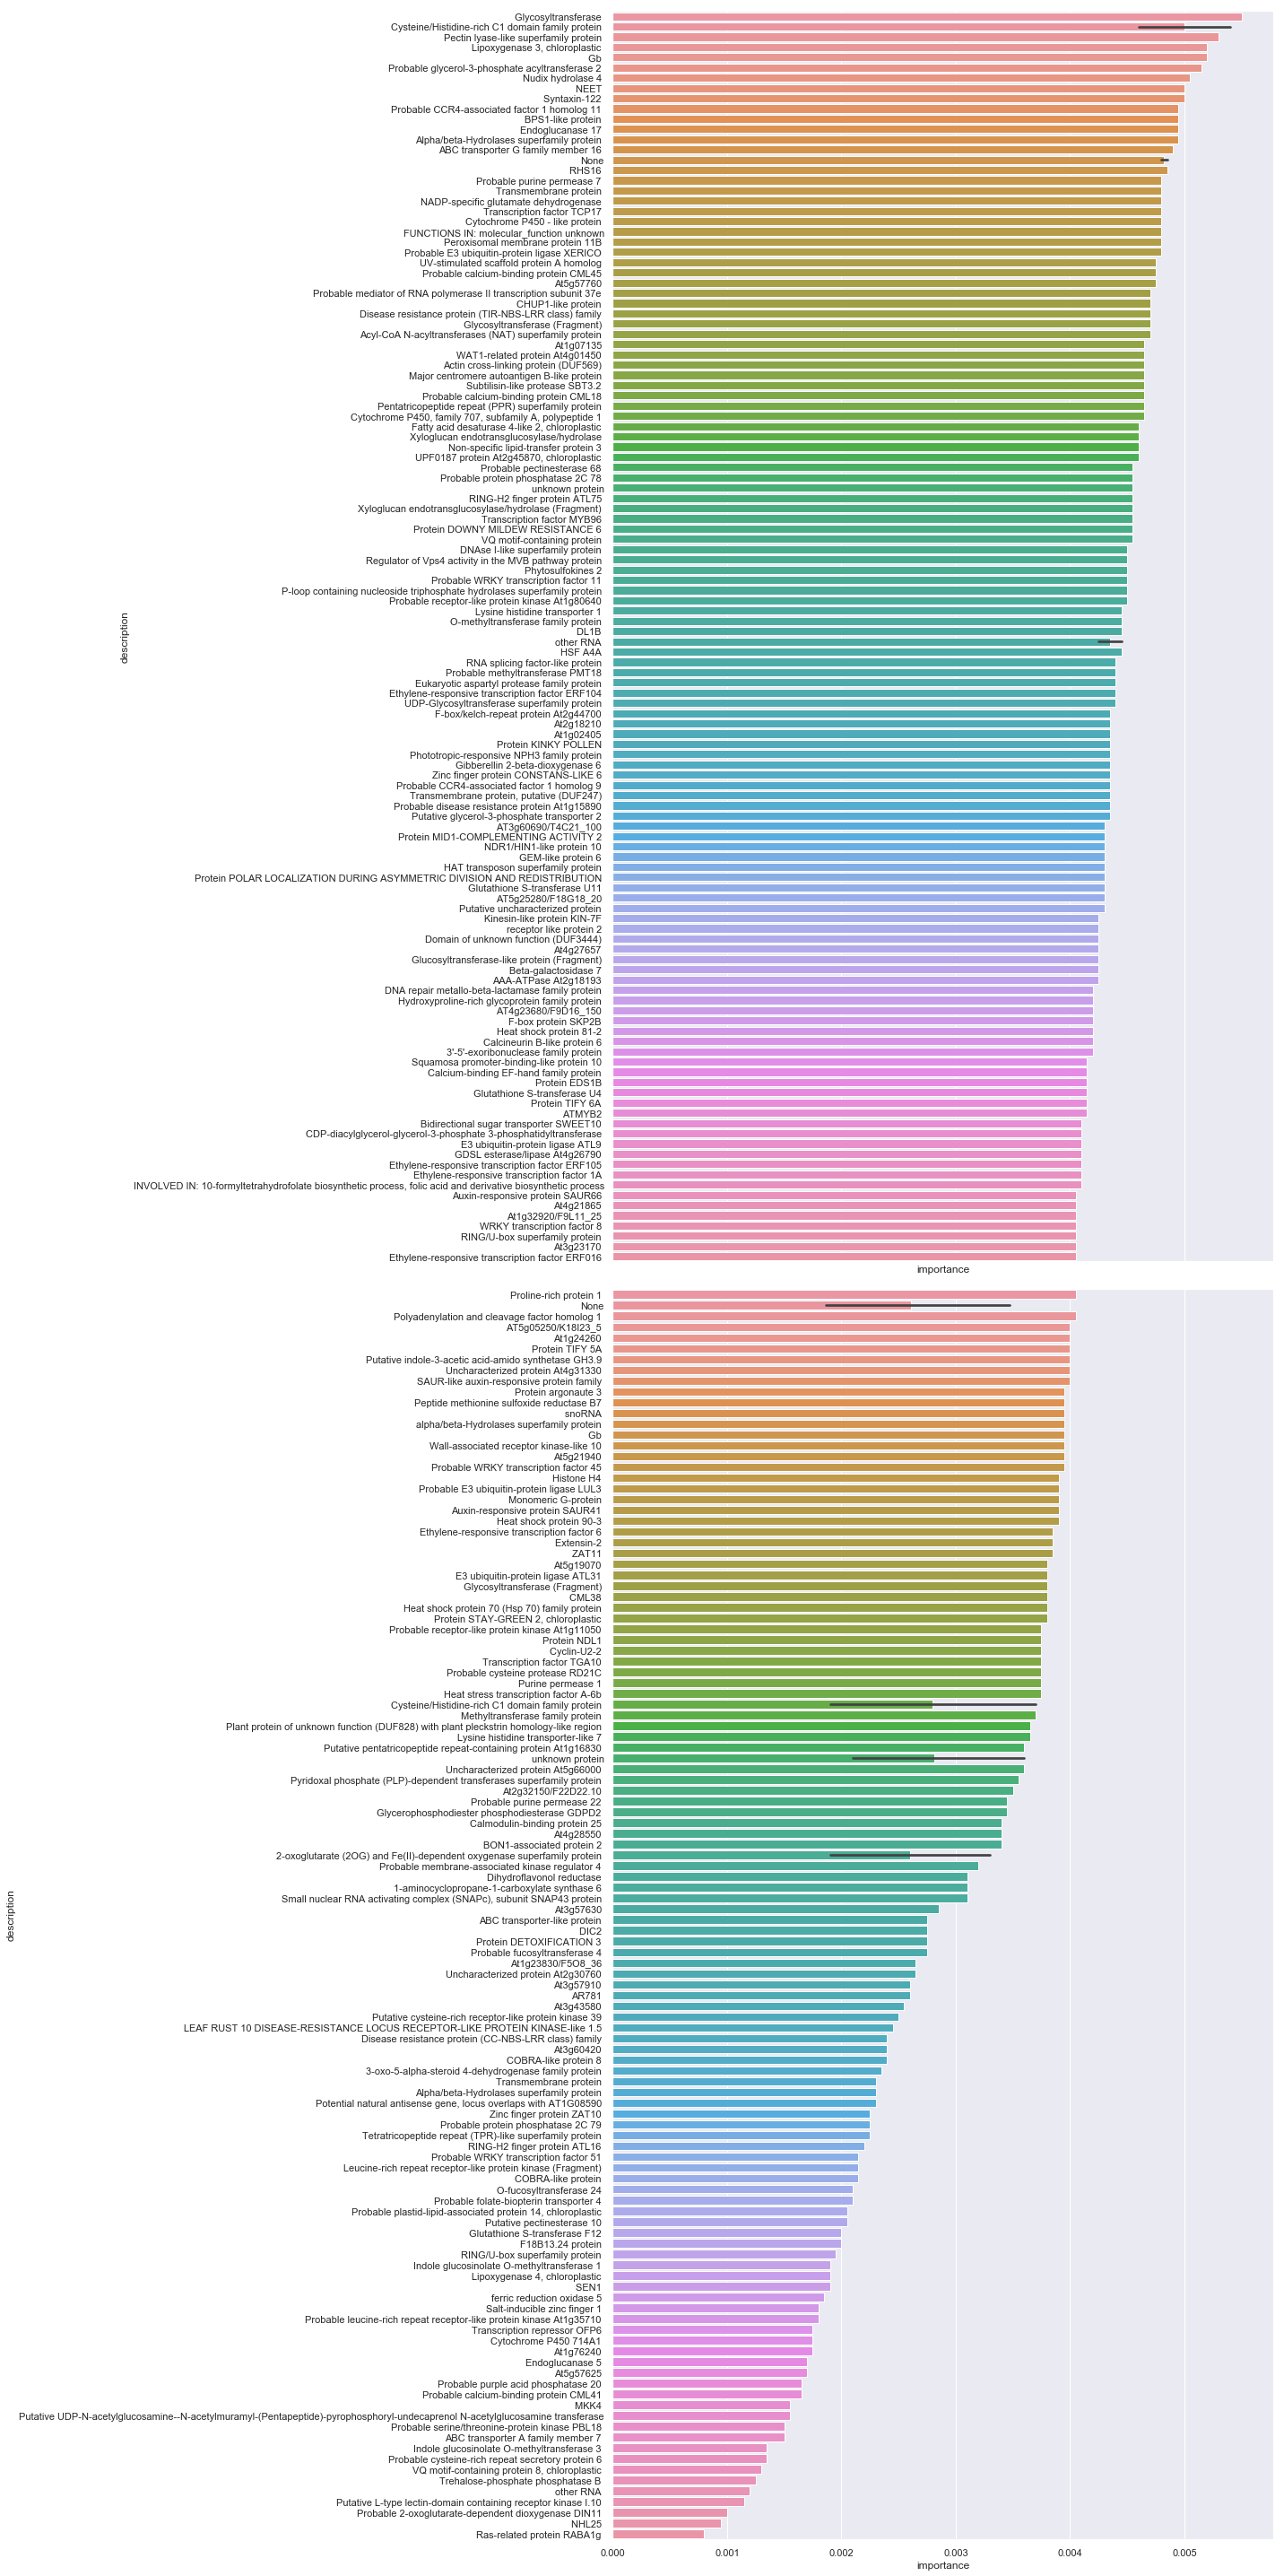
\includegraphics[width=.9\linewidth]{obipy-resources/93e2fbf76ed477962282ae99767b8408de4d3ed9/86df1a6105cefefdce9f5d320820d0043bf1133c.png}
\end{center}





\section{Selecting genes for Col0 at 6hr C/W}
\label{sec:orgfce5a08}
\subsection{RFE selecting 25 genes}
\label{sec:org40e19c7}
\begin{minted}[frame=lines,linenos=true,fontfamily=Monaco]{ipython}
from sklearn.feature_selection import RFE, RFECV
from sklearn.linear_model import LogisticRegression

# load data
DE_pairings_6hr = read_xl('/Users/hughesn/PHD/Transcripts/Data/pairings_6hr.xlsx')
sig = DE_pairings_05hr[DE_pairings_05hr['padj'] < 0.05]
sig = sig['log2FoldChange'].sort_values()
locs = sig.index
df = counts.loc[locs][[c for c in counts.columns if ('6h' in c and 'col' in c)]].T
df = df.loc[:,~df.columns.duplicated()]
df = df[[c for c in set(df.columns.values)]]
\end{minted}

\begin{minted}[frame=lines,linenos=true,fontfamily=Monaco]{ipython}
# Feature Extraction with RFE
X = df.values
y = [y.rsplit('_',1)[0] for y in df.reset_index()['index']]
# feature extraction
model = LogisticRegression()
rfe = RFE(model, n_features_to_select=25)
fit = rfe.fit(X, y)
print("Num Features: {0}".format(fit.n_features_))
print("Selected Features: {0}".format(fit.support_))
print("Feature Ranking: {0}".format(fit.ranking_))
\end{minted}

Num Features: 25\\
Selected Features: [False False False \ldots{} False False False]\\
Feature Ranking: [ 182 1895 5202 \ldots{}  807  973 4321]\\


\begin{minted}[frame=lines,linenos=true,fontfamily=Monaco]{ipython}
genes = []
for r,f in zip(fit.ranking_, df.columns.values):
      if r ==1:
            genes.append(f)
get_gene_names(genes)
\end{minted}

\begin{center}
\begin{tabular}{rlll}
 & incoming & name & description\\
\hline
0 & AT1G18970 & GLP1 & Germin-like protein subfamily T member 1\\
1 & AT3G16420 & PBP1 & PYK10-binding protein 1\\
2 & AT4G39950 & CYP79B2 & cytochrome P450, family 79, subfamily B, polypeptide 2\\
3 & AT2G19970 & AT2G19970 & At2g19970\\
4 & AT1G76680 & OPR1 & 12-oxophytodienoate reductase 1\\
5 & AT3G09260 & BGLU23 & PYK10\\
6 & AT3G28740 & CYP81D11 & Cytochrome P450 81D11\\
7 & AT2G15220 & AT2G15220 & At2g15220/F15A23.4\\
8 & AT1G02930 & GSTF6 & Glutathione S-transferase F6\\
9 & AT5G39580 & PER62 & Peroxidase 62\\
10 & AT2G26560 & PLP2 & Patatin-like protein 2\\
11 & AT5G14650 & AT5G14650 & Pectin lyase-like superfamily protein\\
12 & AT1G26240 & AT1G26240 & Proline-rich extensin-like family protein\\
13 & AT1G09310 & AT1G09310 & T31J12.3 protein\\
14 & AT1G26380 & FOX1 & Berberine bridge enzyme-like 3\\
15 & AT1G02920 & GSTF7 & Glutathione S-transferase F7\\
16 & AT3G16400 & NSP1 & Nitrile-specifier protein 1\\
17 & AT2G27402 & AT2G27402 & At2g27402\\
18 & AT5G20630 & GER3 & Germin-like protein subfamily 3 member 3\\
19 & AT1G66700 & PXMT1 & Paraxanthine methyltransferase 1\\
20 & AT5G13930 & CHS & Chalcone synthase family protein\\
21 & AT3G26830 & CYP71B15 & Bifunctional dihydrocamalexate synthase/camalexin synthase\\
22 & AT5G06730 & PER54 & Peroxidase 54\\
23 & AT5G47500 & PME68 & Probable pectinesterase 68\\
24 & AT5G39110 & AT5G39110 & Germin-like protein subfamily 1 member 14\\
\end{tabular}
\end{center}


\subsubsection{Forest on this RFE set}
\label{sec:org01acb54}

\begin{minted}[frame=lines,linenos=true,fontfamily=Monaco]{ipython}
rfe_forest = counts.loc[genes][[c for c in counts.columns if ('6h' in c and 'col' in c)]].T
rfe_forest = rfe_forest.loc[:,~rfe_forest.columns.duplicated()]
rfe_forest = rfe_forest[[c for c in set(rfe_forest.columns.values)]]

feat_labels = rfe_forest.columns.values
y = [d.rsplit('_', 1)[0] for d in rfe_forest.index.values]

X_train, X_test, y_train, y_test = train_test_split(rfe_forest.values, y, test_size=1, random_state=42)
forest = RandomForestClassifier(n_estimators=20000, random_state=1, n_jobs=-1)
forest.fit(X_train, y_train)
res = {k: v for k, v in sorted(
    zip(feat_labels, forest.feature_importances_), key=lambda x: x[1], reverse=True)}
res_df = pd.DataFrame(list(res.items()), columns=[
                      'gene', 'importance']).set_index('gene')
names = get_gene_names(list(res_df.index))
res_df = pd.merge(res_df, names, left_index=True, right_on='incoming').rename(
    columns={'incoming': 'gene'}).set_index('gene').sort_values('importance', ascending=False)
res_df
\end{minted}

\begin{center}
\begin{tabular}{lrll}
gene & importance & name & description\\
\hline
AT2G26560 & 0.03965 & PLP2 & Patatin-like protein 2\\
AT3G16400 & 0.039 & NSP1 & Nitrile-specifier protein 1\\
AT5G06730 & 0.03815 & PER54 & Peroxidase 54\\
AT2G19970 & 0.03755 & AT2G19970 & At2g19970\\
AT5G47500 & 0.0375 & PME68 & Probable pectinesterase 68\\
AT4G39950 & 0.03745 & CYP79B2 & cytochrome P450, family 79, subfamily B, polypeptide 2\\
AT3G28740 & 0.03725 & CYP81D11 & Cytochrome P450 81D11\\
AT1G18970 & 0.03705 & GLP1 & Germin-like protein subfamily T member 1\\
AT1G76680 & 0.037 & OPR1 & 12-oxophytodienoate reductase 1\\
AT1G26380 & 0.0369 & FOX1 & Berberine bridge enzyme-like 3\\
AT1G02920 & 0.03675 & GSTF7 & Glutathione S-transferase F7\\
AT5G39580 & 0.0366 & PER62 & Peroxidase 62\\
AT3G16420 & 0.03635 & PBP1 & PYK10-binding protein 1\\
AT2G15220 & 0.03625 & AT2G15220 & At2g15220/F15A23.4\\
AT1G09310 & 0.0362 & AT1G09310 & T31J12.3 protein\\
AT5G20630 & 0.0362 & GER3 & Germin-like protein subfamily 3 member 3\\
AT1G66700 & 0.0361 & PXMT1 & Paraxanthine methyltransferase 1\\
AT1G26240 & 0.03585 & AT1G26240 & Proline-rich extensin-like family protein\\
AT1G02930 & 0.0358 & GSTF6 & Glutathione S-transferase F6\\
AT5G13930 & 0.0356 & CHS & Chalcone synthase family protein\\
AT2G27402 & 0.03545 & AT2G27402 & At2g27402\\
AT3G09260 & 0.035 & BGLU23 & PYK10\\
AT5G39110 & 0.03495 & AT5G39110 & Germin-like protein subfamily 1 member 14\\
AT3G26830 & 0.03425 & CYP71B15 & Bifunctional dihydrocamalexate synthase/camalexin synthase\\
AT5G14650 & 0.0341 & AT5G14650 & Pectin lyase-like superfamily protein\\
\end{tabular}
\end{center}

\begin{minted}[frame=lines,linenos=true,fontfamily=Monaco]{ipython}
fig, ax = plt.subplots(1, figsize=(20,20))
sns.barplot(data=res_df.reset_index(), y='description', x='importance', ax=ax)
plt.tight_layout()
\end{minted}

\begin{verbatim}
<Figure size 1440x1440 with 1 Axes>
\end{verbatim}


\begin{center}
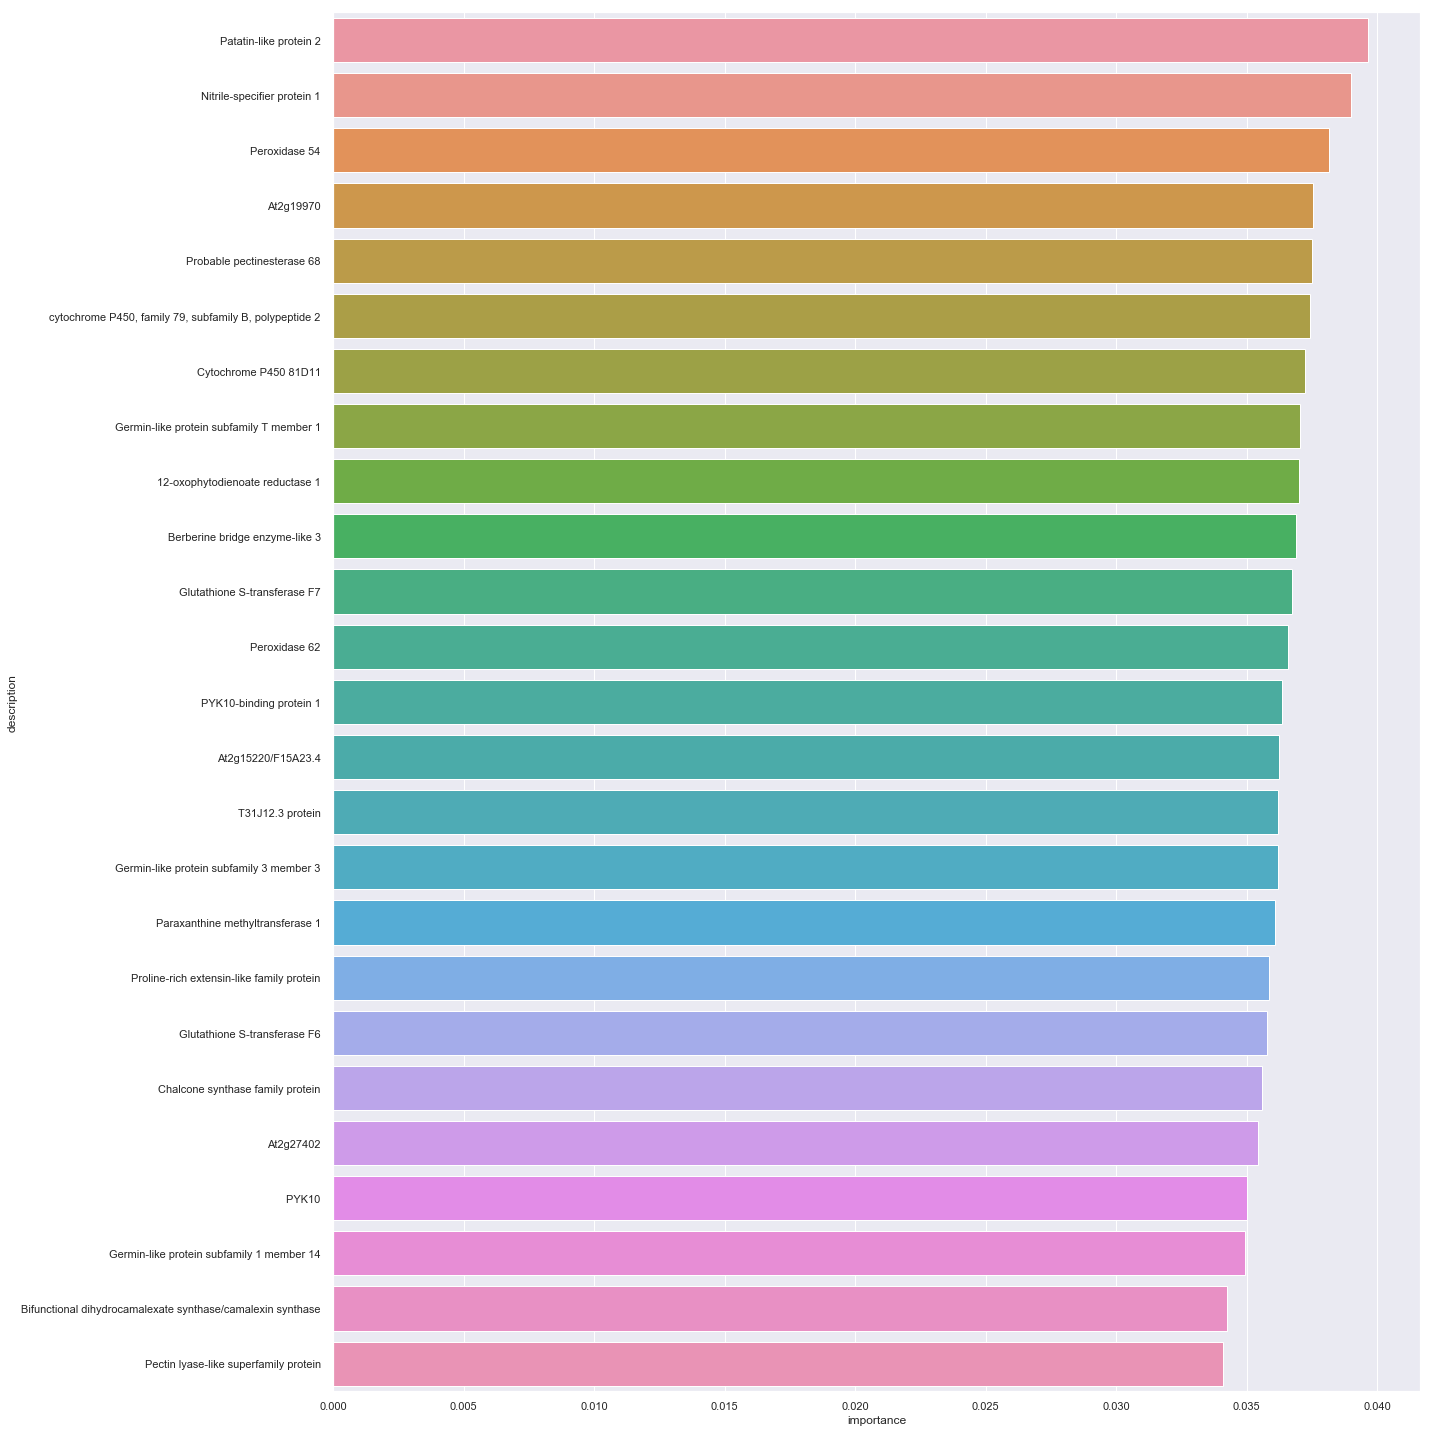
\includegraphics[width=.9\linewidth]{obipy-resources/93e2fbf76ed477962282ae99767b8408de4d3ed9/fc0850005c3f274f6f9419db2a2819926e16f06e.png}
\end{center}


\subsection{RFE selecting 250 genes}
\label{sec:org8232402}
\begin{minted}[frame=lines,linenos=true,fontfamily=Monaco]{ipython}
from sklearn.feature_selection import RFE, RFECV
from sklearn.linear_model import LogisticRegression

# load data
DE_pairings_6hr = read_xl('/Users/hughesn/PHD/Transcripts/Data/pairings_6hr.xlsx')
sig = DE_pairings_05hr[DE_pairings_05hr['padj'] < 0.05]
sig = sig['log2FoldChange'].sort_values()
locs = sig.index
df = counts.loc[locs][[c for c in counts.columns if ('6h' in c and 'col' in c)]].T
df = df.loc[:,~df.columns.duplicated()]
df = df[[c for c in set(df.columns.values)]]
\end{minted}

\begin{minted}[frame=lines,linenos=true,fontfamily=Monaco]{ipython}
# Feature Extraction with RFE
X = df.values
y = [y.rsplit('_',1)[0] for y in df.reset_index()['index']]
# feature extraction
model = LogisticRegression()
rfe = RFE(model, n_features_to_select=250)
fit = rfe.fit(X, y)
print("Num Features: {0}".format(fit.n_features_))
print("Selected Features: {0}".format(fit.support_))
print("Feature Ranking: {0}".format(fit.ranking_))
\end{minted}

Num Features: 250\\
Selected Features: [ True False False \ldots{} False False False]\\
Feature Ranking: [   1 1670 4977 \ldots{}  582  748 4096]\\


\begin{minted}[frame=lines,linenos=true,fontfamily=Monaco]{ipython}
genes = []
for r,f in zip(fit.ranking_, df.columns.values):
      if r ==1:
            genes.append(f)
get_gene_names(genes)
\end{minted}



\begin{center}
\begin{tabular}{rlll}
 & incoming & name & description\\
\hline
0 & AT1G59990 & RH22 & DEAD-box ATP-dependent RNA helicase 22\\
1 & AT1G18970 & GLP1 & Germin-like protein subfamily T member 1\\
2 & AT4G26010 & AT4G26010 & Peroxidase superfamily protein\\
3 & AT1G06002 & AT1G06002 & Potential natural antisense gene, locus overlaps with AT1G06000\\
4 & AT3G01970 & WRKY45 & Probable WRKY transcription factor 45\\
5 & AT5G05735 & AT5G05735 & None\\
6 & AT4G20830 & AT4G20830 & Berberine bridge enzyme-like 19\\
7 & AT5G06865 & AT5G06865 & other RNA\\
8 & AT3G16420 & PBP1 & PYK10-binding protein 1\\
9 & AT4G29390 & RPS30A & 40S ribosomal protein S30\\
10 & AT5G24660 & LSU2 & Protein RESPONSE TO LOW SULFUR 2\\
11 & AT5G58350 & WNK4 & Probable serine/threonine-protein kinase WNK4\\
12 & AT2G24180 & CYP71B6 & Cytochrome P450 71B6\\
13 & AT4G39950 & CYP79B2 & cytochrome P450, family 79, subfamily B, polypeptide 2\\
14 & AT5G19890 & PER59 & Peroxidase 59\\
15 & AT2G10940 & AT2G10940 & At2g10940/F15K19.1\\
16 & AT2G36750 & UGT73C1 & UDP-glycosyltransferase 73C1\\
17 & AT3G04070 & NAC047 & NAC transcription factor 47\\
18 & AT3G21305 & AT3G21305 & None\\
19 & AT3G25700 & AT3G25700 & At3g25700\\
20 & AT2G19970 & AT2G19970 & At2g19970\\
21 & AT1G30530 & UGT78D1 & Glycosyltransferase (Fragment)\\
22 & AT1G76680 & OPR1 & 12-oxophytodienoate reductase 1\\
23 & AT1G18975 & AT1G18975 & None\\
24 & AT3G09260 & BGLU23 & PYK10\\
25 & AT5G57220 & CYP81F2 & Cytochrome P450 81F2\\
26 & AT1G18650 & PDCB3 & PLASMODESMATA CALLOSE-BINDING PROTEIN 3\\
27 & AT5G49480 & ATCP1 & Calcium-binding protein CP1\\
28 & AT4G23700 & CHX17 & Cation/H(+) antiporter 17\\
29 & AT5G64120 & PER71 & Peroxidase\\
30 & AT5G64890 & PEP2 & Elicitor peptide 2\\
31 & AT3G03670 & PER28 & Peroxidase 28\\
32 & AT1G15885 & AT1G15885 & Putative uncharacterized protein\\
33 & AT3G18830 & PLT5 & PMT5\\
34 & AT3G28740 & CYP81D11 & Cytochrome P450 81D11\\
35 & AT3G50480 & HR4 & RPW8-like protein 4\\
36 & AT1G79680 & WAKL10 & Wall-associated receptor kinase-like 10\\
37 & AT1G09750 & AED3 & Aspartyl protease AED3\\
38 & AT2G15220 & AT2G15220 & At2g15220/F15A23.4\\
39 & AT4G02290 & AtGH9B13 & Endoglucanase 17\\
40 & AT1G03220 & AT1G03220 & Eukaryotic aspartyl protease family protein\\
41 & AT1G26410 & FOX4 & Berberine bridge enzyme-like 6\\
42 & AT4G34760 & SAUR50 & Auxin-responsive protein SAUR50\\
43 & AT5G38900 & AT5G38900 & Thioredoxin superfamily protein\\
44 & AT1G14540 & PER4 & Peroxidase\\
45 & AT3G01420 & DOX1 & Alpha-dioxygenase 1\\
46 & AT3G55660 & ROPGEF6 & Rop guanine nucleotide exchange factor 6\\
47 & AT3G51430 & SSL5 & Protein STRICTOSIDINE SYNTHASE-LIKE 5\\
48 & AT1G02930 & GSTF6 & Glutathione S-transferase F6\\
49 & AT2G41810 & AT2G41810 & Uncharacterized protein At2g41810\\
50 & AT1G28290 & AGP31 & Non-classical arabinogalactan protein 31\\
51 & AT4G19420 & AT4G19420 & Pectinacetylesterase family protein\\
52 & AT5G44380 & AT5G44380 & FAD-binding Berberine family protein\\
53 & AT1G26250 & AT1G26250 & Proline-rich extensin-like family protein\\
54 & AT1G02730 & CSLD5 & Cellulose synthase-like protein D5\\
55 & AT4G30720 & AT4G30720 & FAD/NAD(P)-binding oxidoreductase family protein\\
56 & AT2G36690 & AT2G36690 & 2-oxoglutarate (2OG) and Fe(II)-dependent oxygenase superfamily protein\\
57 & AT1G62510 & AT1G62510 & Bifunctional inhibitor/lipid-transfer protein/seed storage 2S albumin superfamily protein\\
58 & AT5G46580 & AT5G46580 & Pentatricopeptide repeat-containing protein At5g46580, chloroplastic\\
59 & AT1G15260 & AT1G15260 & LOW protein: ATP-dependent RNA helicase-like protein\\
60 & AT1G21100 & IGMT1 & Indole glucosinolate O-methyltransferase 1\\
61 & AT4G34950 & AT4G34950 & Major facilitator superfamily protein\\
62 & AT3G09405 & PAE4 & Pectin acetylesterase 4\\
63 & AT5G03390 & AT5G03390 & At5g03390\\
64 & AT2G43120 & AT2G43120 & RmlC-like cupins superfamily protein\\
65 & AT1G21400 & AT1G21400 & Thiamin diphosphate-binding fold (THDP-binding) superfamily protein\\
66 & AT5G42830 & AT5G42830 & HXXXD-type acyl-transferase family protein\\
67 & AT1G67148 & AT1G67148 & Putative uncharacterized protein\\
68 & AT5G52050 & DTX50 & Protein DETOXIFICATION 50\\
69 & AT3G06145 & AT3G06145 & Putative RING zinc finger protein\\
70 & AT3G26210 & CYP71B23 & Cytochrome P450 71B23\\
71 & AT1G65490 & AT1G65490 & unknown protein\\
72 & AT5G48880 & KAT5 & PKT2\\
73 & AT4G25810 & XTH23 & Probable xyloglucan endotransglucosylase/hydrolase protein 23\\
74 & AT2G27389 & AT2G27389 & unknown protein\\
75 & AT5G67400 & PER73 & Peroxidase\\
76 & AT5G55580 & MTERF9 & Transcription termination factor MTERF9, chloroplastic\\
77 & AT5G05730 & ASA1 & Anthranilate synthase alpha subunit 1\\
78 & AT5G26340 & STP13 & STP13\\
79 & AT4G21760 & BGLU47 & beta-glucosidase 47\\
80 & AT1G48570 & AT1G48570 & T1N15.19\\
81 & AT5G54810 & TSB1 & Tryptophan synthase\\
82 & AT1G67980 & CCOAMT & Putative caffeoyl-CoA O-methyltransferase At1g67980\\
83 & AT5G14330 & AT5G14330 & Transmembrane protein\\
84 & AT4G19370 & AT4G19370 & Chitin synthase, putative (DUF1218)\\
85 & AT5G13080 & WRKY75 & WRKY75\\
86 & AT1G03630 & PORC & Protochlorophyllide reductase C, chloroplastic\\
87 & AT2G27710 & RPP2B & AT2G27710 protein\\
88 & AT4G21770 & AT4G21770 & RNA pseudouridine synthase 6, chloroplastic\\
89 & AT1G69490 & NAC029 & NAP\\
90 & AT5G39580 & PER62 & Peroxidase 62\\
91 & AT3G54580 & AT3G54580 & Proline-rich extensin-like family protein\\
92 & AT5G11550 & AT5G11550 & ARM repeat superfamily protein\\
93 & AT4G15610 & AT4G15610 & CASP-like protein 1D1\\
94 & AT1G64160 & DIR5 & Dirigent protein 5\\
95 & AT5G49330 & MYB111 & Transcription factor MYB111\\
96 & AT3G48850 & MPT2 & Mitochondrial phosphate carrier protein 2, mitochondrial\\
97 & AT4G37540 & LBD39 & LOB domain-containing protein 39\\
98 & AT2G26560 & PLP2 & Patatin-like protein 2\\
99 & AT5G58250 & AT5G58250 & YCF54\\
100 & AT4G01037 & WTF1 & WTF1\\
101 & AT3G48500 & PDE312 & Nucleic acid-binding, OB-fold-like protein\\
102 & AT3G13950 & AT3G13950 & AT3G13950 protein\\
103 & AT4G09040 & AT4G09040 & At4g09040\\
104 & AT2G19990 & PR-1-LIKE & PR-1-like protein\\
105 & AT2G12170 & AT2G12170 & BEST Arabidopsis thaliana protein match is: Transcriptional factor B3 family protein (TAIR:AT2G24645.1)\\
106 & AT5G14650 & AT5G14650 & Pectin lyase-like superfamily protein\\
107 & AT3G52450 & PUB22 & RING-type E3 ubiquitin transferase\\
108 & AT5G56670 & RPS30A & 40S ribosomal protein S30\\
109 & AT1G26240 & AT1G26240 & Proline-rich extensin-like family protein\\
110 & AT3G63380 & ACA12 & Calcium-transporting ATPase\\
111 & AT2G38870 & AT2G38870 & Putative protease inhibitor\\
112 & AT5G23310 & FSD3 & Superoxide dismutase\\
113 & AT4G24780 & AT4G24780 & Probable pectate lyase 18\\
114 & AT1G10522 & PRIN2 & Protein PLASTID REDOX INSENSITIVE 2, chloroplastic\\
115 & AT3G14900 & AT3G14900 & Uncharacterized protein At3g14900\\
116 & AT4G28420 & AT4G28420 & Probable aminotransferase TAT1\\
117 & AT2G24850 & TAT3 & Probable aminotransferase TAT3\\
118 & AT2G46840 & DUF4 & DUF4\\
119 & AT4G02520 & GSTF2 & Glutathione S-transferase F2\\
120 & AT1G09310 & AT1G09310 & T31J12.3 protein\\
121 & AT4G35730 & AT4G35730 & Regulator of Vps4 activity in the MVB pathway protein\\
122 & AT1G51700 & DOF1.7 & Dof zinc finger protein DOF1.7\\
123 & AT1G05523 & AT1G05523 & None\\
124 & AT3G24300 & AMT1-3 & Ammonium transporter 1 member 3\\
125 & AT4G14630 & GLP9 & At4g14630\\
126 & AT4G00050 & UNE10 & Transcription factor UNE10\\
127 & AT1G26380 & FOX1 & Berberine bridge enzyme-like 3\\
128 & AT1G02920 & GSTF7 & Glutathione S-transferase F7\\
129 & AT5G15780 & AT5G15780 & At5g15780\\
130 & AT3G25790 & HHO1 & Transcription factor HHO1\\
131 & AT3G18420 & SG1 & protein SLOW GREEN 1, chloroplastic\\
132 & AT4G02510 & TOC159 & Translocase of chloroplast 159, chloroplastic\\
133 & AT4G18730 & RPL11C & 60S ribosomal protein L11-2\\
134 & AT3G58990 & IPMI1 & 3-isopropylmalate dehydratase small subunit 2\\
135 & AT5G02780 & GSTL1 & Glutathione S-transferase L1\\
136 & AT1G13930 & AT1G13930 & At1g13930/F16A14.27\\
137 & AT1G69200 & FLN2 & Fructokinase-like 2, chloroplastic\\
138 & AT4G25740 & RPS10A & 40S ribosomal protein S10-1\\
139 & AT5G55280 & FTSZ1 & Cell division protein FtsZ homolog 1, chloroplastic\\
140 & AT1G29720 & RFK1 & Probable LRR receptor-like serine/threonine-protein kinase At1g29720\\
141 & AT5G40780 & LHT1 & Lysine histidine transporter 1\\
142 & AT5G66530 & AT5G66530 & Glucose-6-phosphate 1-epimerase\\
143 & AT5G06860 & PGIP1 & PGIP1\\
144 & AT3G16400 & NSP1 & Nitrile-specifier protein 1\\
145 & AT3G56090 & FER3 & Ferritin-3, chloroplastic\\
146 & AT2G27402 & AT2G27402 & At2g27402\\
147 & AT5G40730 & AGP24 & Arabinogalactan peptide 24\\
148 & AT5G20230 & BCB & SAG14\\
149 & AT1G30700 & AT1G30700 & Berberine bridge enzyme-like 8\\
150 & AT5G20790 & AT5G20790 & unknown protein\\
151 & AT3G62530 & AT3G62530 & ARM repeat superfamily protein\\
152 & AT2G17740 & AT2G17740 & At2g17740\\
153 & AT2G41310 & ARR8 & Two-component response regulator ARR8\\
154 & AT4G37370 & CYP81D8 & Cytochrome P450, family 81, subfamily D, polypeptide 8\\
155 & AT5G51720 & NEET & NEET\\
156 & AT1G55020 & LOX1 & Linoleate 9S-lipoxygenase 1\\
157 & AT1G08757 & AT1G08757 & None\\
158 & AT1G52245 & AT1G52245 & Dynein light chain\\
159 & AT1G71695 & PER12 & Peroxidase\\
160 & AT5G44990 & AT5G44990 & Glutathione S-transferase family protein\\
161 & AT3G45030 & RPS20C & 40S ribosomal protein S20-1\\
162 & AT1G65690 & NHL6 & NDR1/HIN1-like protein 6\\
163 & AT1G26255 & AT1G26255 & None\\
164 & AT4G02270 & RHS13 & At4g02270\\
165 & AT4G00360 & CYP86A2 & Cytochrome P450 86A2\\
166 & AT2G02100 & PDF2.2 & PDF2.2\\
167 & AT3G50770 & CML41 & Probable calcium-binding protein CML41\\
168 & AT4G26150 & GATA22 & Putative GATA transcription factor 22\\
169 & AT2G29150 & AT2G29150 & Tropinone reductase homolog At2g29150\\
170 & AT2G32990 & AtGH9B8 & Endoglucanase 11\\
171 & AT5G20630 & GER3 & Germin-like protein subfamily 3 member 3\\
172 & AT5G08610 & RH26 & PDE340\\
173 & AT3G05730 & AT3G05730 & Defensin-like protein 205\\
174 & AT3G44860 & FAMT & Farnesoic acid carboxyl-O-methyltransferase\\
175 & AT1G13520 & AT1G13520 & At1g13520\\
176 & AT1G08380 & PSAO & PSAO\\
177 & AT5G63140 & PAP29 & Probable inactive purple acid phosphatase 29\\
178 & AT5G66470 & AT5G66470 & GTPase ERA-like, chloroplastic\\
179 & AT1G02660 & PLIP2 & Phospholipase A1 PLIP2, chloroplastic\\
180 & AT1G78450 & AT1G78450 & F3F9.4\\
181 & AT5G19750 & AT5G19750 & Peroxisomal membrane 22 kDa (Mpv17/PMP22) family protein\\
182 & AT5G64040 & PSAN & Photosystem I reaction center subunit PSI-N, chloroplast, putative / PSI-N, putative (PSAN)\\
183 & AT4G29740 & CKX4 & Cytokinin dehydrogenase 4\\
184 & AT1G18250 & ATLP-1 & Pathogenesis-related thaumatin superfamily protein\\
185 & AT3G18250 & AT3G18250 & Putative membrane lipoprotein\\
186 & AT3G16670 & AT3G16670 & AT3g16670/MGL6\_12\\
187 & AT1G18980 & AT1G18980 & At1g18980\\
188 & AT4G34290 & AT4G34290 & SWIB/MDM2 domain superfamily protein\\
189 & AT3G46280 & AT3G46280 & Kinase-like protein\\
190 & AT4G20835 & AT4G20835 & None\\
191 & AT1G66700 & PXMT1 & Paraxanthine methyltransferase 1\\
192 & AT3G26445 & AT3G26445 & Beta-1,4-N-acetylglucosaminyltransferase family protein\\
193 & AT5G26920 & CBP60G & Calmodulin-binding protein 60 G\\
194 & AT5G16980 & AT5G16980 & Zinc-binding dehydrogenase family protein\\
195 & AT4G10530 & AT4G10530 & Subtilase family protein\\
196 & AT3G54890 & LHCA1 & Chlorophyll a-b binding protein, chloroplastic\\
197 & AT2G28000 & CPN60A1 & SLP\\
198 & AT4G24240 & WRKY7 & Probable WRKY transcription factor 7\\
199 & AT2G41380 & AT2G41380 & At2g41380\\
200 & AT1G18570 & MYB51 & Transcription factor MYB51\\
201 & AT3G56070 & CYP19-3 & Peptidyl-prolyl cis-trans isomerase CYP19-3\\
202 & AT5G08640 & FLS1 & Flavonol synthase/flavanone 3-hydroxylase\\
203 & AT1G06000 & UGT89C1 & Glycosyltransferase (Fragment)\\
204 & AT4G30090 & AT4G30090 & Golgin family A protein\\
205 & AT5G56870 & BGAL4 & Beta-galactosidase 4\\
206 & AT5G42650 & CYP74A & Allene oxide synthase, chloroplastic\\
207 & AT4G29905 & AT4G29905 & Putative uncharacterized protein\\
208 & AT2G46750 & GULLO2 & L-gulonolactone oxidase 2\\
209 & AT5G13930 & CHS & Chalcone synthase family protein\\
210 & AT3G26830 & CYP71B15 & Bifunctional dihydrocamalexate synthase/camalexin synthase\\
211 & AT2G45870 & AT2G45870 & UPF0187 protein At2g45870, chloroplastic\\
212 & AT1G32640 & MYC2 & ZBF1\\
213 & AT4G03985 & AT4G03985 & None\\
214 & AT4G12320 & CYP706A6 & At4g12320\\
215 & AT2G28740 & HIS4 & Histone H4\\
216 & AT2G25297 & AT2G25297 & None\\
217 & AT5G06730 & PER54 & Peroxidase 54\\
218 & AT1G26420 & FOX5 & Berberine bridge enzyme-like 7\\
219 & AT5G48657 & AT5G48657 & defense protein-related\\
220 & AT1G11300 & AT1G11300 & G-type lectin S-receptor-like serine/threonine-protein kinase At1g11300\\
221 & AT4G32260 & AT4G32260 & PDE334\\
222 & AT2G32650 & AT2G32650 & At2g32650\\
223 & AT1G21120 & AT1G21120 & O-methyltransferase family protein\\
224 & AT1G72600 & AT1G72600 & At1g72600\\
225 & AT5G08070 & TCP17 & Transcription factor TCP17\\
226 & AT5G57625 & AT5G57625 & At5g57625\\
227 & AT1G67030 & ZFP6 & Zinc finger protein 6\\
228 & AT1G72610 & GLP1 & Germin-like protein subfamily 3 member 1\\
229 & AT2G02930 & GSTF3 & Glutathione S-transferase F3\\
230 & AT5G47500 & PME68 & Probable pectinesterase 68\\
231 & AT5G07030 & AT5G07030 & Eukaryotic aspartyl protease family protein\\
232 & AT1G80850 & AT1G80850 & At1g80850\\
233 & AT1G51890 & AT1G51890 & Leucine-rich repeat protein kinase family protein\\
234 & AT2G18690 & AT2G18690 & Expressed protein\\
235 & AT2G48130 & AT2G48130 & Bifunctional inhibitor/lipid-transfer protein/seed storage 2S albumin superfamily protein\\
236 & AT4G14780 & AT4G14780 & Kinase like protein\\
237 & AT2G34180 & CIPK13 & CBL-interacting serine/threonine-protein kinase 13\\
238 & AT4G15530 & PPDK & Pyruvate, phosphate dikinase 1, chloroplastic\\
239 & AT1G32350 & AOX3 & AOX1D\\
240 & AT1G07590 & AT1G07590 & Pentatricopeptide repeat-containing protein At1g07590, mitochondrial\\
241 & AT5G26290 & AT5G26290 & TRAF-like family protein\\
242 & AT5G11210 & GLR2.5 & Glutamate receptor 2.5\\
243 & AT4G24110 & AT4G24110 & NADP-specific glutamate dehydrogenase\\
244 & AT4G01700 & AT4G01700 & At4g01700\\
245 & AT4G31500 & CYP83B1 & Cytochrome P450 83B1\\
246 & AT1G14870 & PCR2 & PCR2\\
247 & AT2G39670 & AT2G39670 & Radical SAM superfamily protein\\
248 & AT3G12930 & IJ & Protein Iojap, chloroplastic\\
249 & AT5G39110 & AT5G39110 & Germin-like protein subfamily 1 member 14\\
\end{tabular}
\end{center}


\paragraph{Forest on this RFE set}
\label{sec:org44d5e63}

\begin{minted}[frame=lines,linenos=true,fontfamily=Monaco]{ipython}
rfe_forest = counts.loc[genes][[c for c in counts.columns if ('6h' in c and 'col' in c)]].T
rfe_forest = rfe_forest.loc[:,~rfe_forest.columns.duplicated()]
rfe_forest = rfe_forest[[c for c in set(rfe_forest.columns.values)]]

feat_labels = rfe_forest.columns.values
y = [d.rsplit('_', 1)[0] for d in rfe_forest.index.values]

X_train, X_test, y_train, y_test = train_test_split(rfe_forest.values, y, test_size=1, random_state=42)
forest = RandomForestClassifier(n_estimators=20000, random_state=1, n_jobs=-1)
forest.fit(X_train, y_train)
res = {k: v for k, v in sorted(
    zip(feat_labels, forest.feature_importances_), key=lambda x: x[1], reverse=True)}
res_df = pd.DataFrame(list(res.items()), columns=[
                      'gene', 'importance']).set_index('gene')
names = get_gene_names(list(res_df.index))
res_df = pd.merge(res_df, names, left_index=True, right_on='incoming').rename(
    columns={'incoming': 'gene'}).set_index('gene').sort_values('importance', ascending=False)
res_df
\end{minted}

\begin{center}
\begin{tabular}{lrll}
gene & importance & name & description\\
\hline
AT1G32640 & 0.0049 & MYC2 & ZBF1\\
AT1G18250 & 0.0048 & ATLP-1 & Pathogenesis-related thaumatin superfamily protein\\
AT4G03985 & 0.0046 & AT4G03985 & None\\
AT2G36690 & 0.0045 & AT2G36690 & 2-oxoglutarate (2OG) and Fe(II)-dependent oxygenase superfamily protein\\
AT1G07590 & 0.0045 & AT1G07590 & Pentatricopeptide repeat-containing protein At1g07590, mitochondrial\\
AT2G27389 & 0.0045 & AT2G27389 & unknown protein\\
AT2G45870 & 0.00445 & AT2G45870 & UPF0187 protein At2g45870, chloroplastic\\
AT4G26010 & 0.00445 & AT4G26010 & Peroxidase superfamily protein\\
AT4G00360 & 0.0044 & CYP86A2 & Cytochrome P450 86A2\\
AT3G01970 & 0.0044 & WRKY45 & Probable WRKY transcription factor 45\\
AT3G06145 & 0.00435 & AT3G06145 & Putative RING zinc finger protein\\
AT5G56670 & 0.00435 & RPS30A & 40S ribosomal protein S30\\
AT4G34950 & 0.00435 & AT4G34950 & Major facilitator superfamily protein\\
AT5G63140 & 0.00435 & PAP29 & Probable inactive purple acid phosphatase 29\\
AT5G56870 & 0.00435 & BGAL4 & Beta-galactosidase 4\\
AT5G11550 & 0.00435 & AT5G11550 & ARM repeat superfamily protein\\
AT1G67148 & 0.00435 & AT1G67148 & Putative uncharacterized protein\\
AT5G49330 & 0.0043 & MYB111 & Transcription factor MYB111\\
AT2G19990 & 0.0043 & PR-1-LIKE & PR-1-like protein\\
AT3G05730 & 0.0043 & AT3G05730 & Defensin-like protein 205\\
AT1G67030 & 0.0043 & ZFP6 & Zinc finger protein 6\\
AT3G56090 & 0.0043 & FER3 & Ferritin-3, chloroplastic\\
AT3G52450 & 0.00425 & PUB22 & RING-type E3 ubiquitin transferase\\
AT2G32990 & 0.00425 & AtGH9B8 & Endoglucanase 11\\
AT2G19970 & 0.00425 & AT2G19970 & At2g19970\\
AT4G37370 & 0.00425 & CYP81D8 & Cytochrome P450, family 81, subfamily D, polypeptide 8\\
AT1G72600 & 0.00425 & AT1G72600 & At1g72600\\
AT1G51700 & 0.00425 & DOF1.7 & Dof zinc finger protein DOF1.7\\
AT3G26830 & 0.0042 & CYP71B15 & Bifunctional dihydrocamalexate synthase/camalexin synthase\\
AT3G28740 & 0.0042 & CYP81D11 & Cytochrome P450 81D11\\
AT2G18690 & 0.0042 & AT2G18690 & Expressed protein\\
AT3G50480 & 0.0042 & HR4 & RPW8-like protein 4\\
AT5G06730 & 0.0042 & PER54 & Peroxidase 54\\
AT4G25810 & 0.00415 & XTH23 & Probable xyloglucan endotransglucosylase/hydrolase protein 23\\
AT3G24300 & 0.0041 & AMT1-3 & Ammonium transporter 1 member 3\\
AT4G02510 & 0.0041 & TOC159 & Translocase of chloroplast 159, chloroplastic\\
AT1G65490 & 0.0041 & AT1G65490 & unknown protein\\
AT2G27402 & 0.0041 & AT2G27402 & At2g27402\\
AT1G55020 & 0.0041 & LOX1 & Linoleate 9S-lipoxygenase 1\\
AT4G23700 & 0.0041 & CHX17 & Cation/H(+) antiporter 17\\
AT5G08070 & 0.0041 & TCP17 & Transcription factor TCP17\\
AT4G00050 & 0.0041 & UNE10 & Transcription factor UNE10\\
AT5G47500 & 0.0041 & PME68 & Probable pectinesterase 68\\
AT2G15220 & 0.00405 & AT2G15220 & At2g15220/F15A23.4\\
AT4G25740 & 0.00405 & RPS10A & 40S ribosomal protein S10-1\\
AT4G14630 & 0.00405 & GLP9 & At4g14630\\
AT3G18250 & 0.00405 & AT3G18250 & Putative membrane lipoprotein\\
AT1G02930 & 0.00405 & GSTF6 & Glutathione S-transferase F6\\
AT3G56070 & 0.004 & CYP19-3 & Peptidyl-prolyl cis-trans isomerase CYP19-3\\
AT3G04070 & 0.004 & NAC047 & NAC transcription factor 47\\
AT4G02520 & 0.004 & GSTF2 & Glutathione S-transferase F2\\
AT3G25790 & 0.004 & HHO1 & Transcription factor HHO1\\
AT5G16980 & 0.004 & AT5G16980 & Zinc-binding dehydrogenase family protein\\
AT1G18650 & 0.004 & PDCB3 & PLASMODESMATA CALLOSE-BINDING PROTEIN 3\\
AT2G29150 & 0.004 & AT2G29150 & Tropinone reductase homolog At2g29150\\
AT1G18570 & 0.004 & MYB51 & Transcription factor MYB51\\
AT3G09405 & 0.004 & PAE4 & Pectin acetylesterase 4\\
AT5G64890 & 0.004 & PEP2 & Elicitor peptide 2\\
AT2G25297 & 0.004 & AT2G25297 & None\\
AT1G26410 & 0.004 & FOX4 & Berberine bridge enzyme-like 6\\
AT3G26445 & 0.004 & AT3G26445 & Beta-1,4-N-acetylglucosaminyltransferase family protein\\
AT3G48850 & 0.004 & MPT2 & Mitochondrial phosphate carrier protein 2, mitochondrial\\
AT1G59990 & 0.004 & RH22 & DEAD-box ATP-dependent RNA helicase 22\\
AT2G34180 & 0.004 & CIPK13 & CBL-interacting serine/threonine-protein kinase 13\\
AT5G40780 & 0.00395 & LHT1 & Lysine histidine transporter 1\\
AT4G21770 & 0.00395 & AT4G21770 & RNA pseudouridine synthase 6, chloroplastic\\
AT1G02660 & 0.00395 & PLIP2 & Phospholipase A1 PLIP2, chloroplastic\\
AT5G44380 & 0.00395 & AT5G44380 & FAD-binding Berberine family protein\\
AT3G58990 & 0.00395 & IPMI1 & 3-isopropylmalate dehydratase small subunit 2\\
AT1G18980 & 0.00395 & AT1G18980 & At1g18980\\
AT1G48570 & 0.00395 & AT1G48570 & T1N15.19\\
AT5G23310 & 0.00395 & FSD3 & Superoxide dismutase\\
AT2G39670 & 0.0039 & AT2G39670 & Radical SAM superfamily protein\\
AT1G13520 & 0.0039 & AT1G13520 & At1g13520\\
AT5G49480 & 0.0039 & ATCP1 & Calcium-binding protein CP1\\
AT3G48500 & 0.0039 & PDE312 & Nucleic acid-binding, OB-fold-like protein\\
AT1G72610 & 0.0039 & GLP1 & Germin-like protein subfamily 3 member 1\\
AT1G30700 & 0.0039 & AT1G30700 & Berberine bridge enzyme-like 8\\
AT5G19890 & 0.0039 & PER59 & Peroxidase 59\\
AT1G64160 & 0.0039 & DIR5 & Dirigent protein 5\\
AT4G29905 & 0.0039 & AT4G29905 & Putative uncharacterized protein\\
AT3G14900 & 0.0039 & AT3G14900 & Uncharacterized protein At3g14900\\
AT2G26560 & 0.0039 & PLP2 & Patatin-like protein 2\\
AT4G18730 & 0.0039 & RPL11C & 60S ribosomal protein L11-2\\
AT5G08610 & 0.0039 & RH26 & PDE340\\
AT2G28740 & 0.0039 & HIS4 & Histone H4\\
AT5G06865 & 0.00385 & AT5G06865 & other RNA\\
AT1G26250 & 0.00385 & AT1G26250 & Proline-rich extensin-like family protein\\
AT3G16420 & 0.00385 & PBP1 & PYK10-binding protein 1\\
AT4G39950 & 0.0038 & CYP79B2 & cytochrome P450, family 79, subfamily B, polypeptide 2\\
AT5G48880 & 0.0038 & KAT5 & PKT2\\
AT1G09750 & 0.0038 & AED3 & Aspartyl protease AED3\\
AT4G10530 & 0.0038 & AT4G10530 & Subtilase family protein\\
AT5G20630 & 0.0038 & GER3 & Germin-like protein subfamily 3 member 3\\
AT1G69200 & 0.0038 & FLN2 & Fructokinase-like 2, chloroplastic\\
AT5G66470 & 0.0038 & AT5G66470 & GTPase ERA-like, chloroplastic\\
AT3G21305 & 0.0038 & AT3G21305 & None\\
AT2G41310 & 0.0038 & ARR8 & Two-component response regulator ARR8\\
AT1G26255 & 0.0038 & AT1G26255 & None\\
AT4G26150 & 0.0038 & GATA22 & Putative GATA transcription factor 22\\
AT4G14780 & 0.00375 & AT4G14780 & Kinase like protein\\
AT1G08757 & 0.00375 & AT1G08757 & None\\
AT2G12170 & 0.00375 & AT2G12170 & BEST Arabidopsis thaliana protein match is: Transcriptional factor B3 family protein (TAIR:AT2G24645.1)\\
AT5G26290 & 0.00375 & AT5G26290 & TRAF-like family protein\\
AT2G02930 & 0.00375 & GSTF3 & Glutathione S-transferase F3\\
AT2G38870 & 0.00375 & AT2G38870 & Putative protease inhibitor\\
AT4G15610 & 0.00375 & AT4G15610 & CASP-like protein 1D1\\
AT4G21760 & 0.00375 & BGLU47 & beta-glucosidase 47\\
AT3G62530 & 0.00375 & AT3G62530 & ARM repeat superfamily protein\\
AT1G52245 & 0.00375 & AT1G52245 & Dynein light chain\\
AT4G12320 & 0.0037 & CYP706A6 & At4g12320\\
AT3G51430 & 0.0037 & SSL5 & Protein STRICTOSIDINE SYNTHASE-LIKE 5\\
AT5G11210 & 0.0037 & GLR2.5 & Glutamate receptor 2.5\\
AT1G02920 & 0.0037 & GSTF7 & Glutathione S-transferase F7\\
AT5G26920 & 0.0037 & CBP60G & Calmodulin-binding protein 60 G\\
AT5G58250 & 0.0037 & AT5G58250 & YCF54\\
AT4G37540 & 0.0037 & LBD39 & LOB domain-containing protein 39\\
AT2G17740 & 0.0037 & AT2G17740 & At2g17740\\
AT1G26420 & 0.00365 & FOX5 & Berberine bridge enzyme-like 7\\
AT4G24240 & 0.00365 & WRKY7 & Probable WRKY transcription factor 7\\
AT3G12930 & 0.00365 & IJ & Protein Iojap, chloroplastic\\
AT1G79680 & 0.00365 & WAKL10 & Wall-associated receptor kinase-like 10\\
AT5G51720 & 0.00365 & NEET & NEET\\
AT5G14330 & 0.00365 & AT5G14330 & Transmembrane protein\\
AT3G26210 & 0.00365 & CYP71B23 & Cytochrome P450 71B23\\
AT1G14870 & 0.00365 & PCR2 & PCR2\\
AT1G71695 & 0.00365 & PER12 & Peroxidase\\
AT5G52050 & 0.00365 & DTX50 & Protein DETOXIFICATION 50\\
AT1G76680 & 0.00365 & OPR1 & 12-oxophytodienoate reductase 1\\
AT3G16670 & 0.00365 & AT3G16670 & AT3g16670/MGL6\_12\\
AT2G32650 & 0.00365 & AT2G32650 & At2g32650\\
AT3G46280 & 0.00365 & AT3G46280 & Kinase-like protein\\
AT1G32350 & 0.0036 & AOX3 & AOX1D\\
AT1G69490 & 0.0036 & NAC029 & NAP\\
AT5G20790 & 0.0036 & AT5G20790 & unknown protein\\
AT5G38900 & 0.0036 & AT5G38900 & Thioredoxin superfamily protein\\
AT3G18830 & 0.0036 & PLT5 & PMT5\\
AT1G03630 & 0.0036 & PORC & Protochlorophyllide reductase C, chloroplastic\\
AT2G27710 & 0.0036 & RPP2B & AT2G27710 protein\\
AT5G02780 & 0.0036 & GSTL1 & Glutathione S-transferase L1\\
AT4G24110 & 0.0036 & AT4G24110 & NADP-specific glutamate dehydrogenase\\
AT1G06000 & 0.0036 & UGT89C1 & Glycosyltransferase (Fragment)\\
AT1G29720 & 0.0036 & RFK1 & Probable LRR receptor-like serine/threonine-protein kinase At1g29720\\
AT1G30530 & 0.0036 & UGT78D1 & Glycosyltransferase (Fragment)\\
AT5G67400 & 0.0036 & PER73 & Peroxidase\\
AT1G10522 & 0.0036 & PRIN2 & Protein PLASTID REDOX INSENSITIVE 2, chloroplastic\\
AT4G02290 & 0.00355 & AtGH9B13 & Endoglucanase 17\\
AT4G29390 & 0.00355 & RPS30A & 40S ribosomal protein S30\\
AT1G78450 & 0.00355 & AT1G78450 & F3F9.4\\
AT5G05730 & 0.00355 & ASA1 & Anthranilate synthase alpha subunit 1\\
AT5G20230 & 0.00355 & BCB & SAG14\\
AT5G03390 & 0.00355 & AT5G03390 & At5g03390\\
AT1G67980 & 0.00355 & CCOAMT & Putative caffeoyl-CoA O-methyltransferase At1g67980\\
AT2G24180 & 0.00355 & CYP71B6 & Cytochrome P450 71B6\\
AT4G30720 & 0.0035 & AT4G30720 & FAD/NAD(P)-binding oxidoreductase family protein\\
AT1G14540 & 0.0035 & PER4 & Peroxidase\\
AT5G42830 & 0.0035 & AT5G42830 & HXXXD-type acyl-transferase family protein\\
AT1G21400 & 0.0035 & AT1G21400 & Thiamin diphosphate-binding fold (THDP-binding) superfamily protein\\
AT5G48657 & 0.0035 & AT5G48657 & defense protein-related\\
AT5G08640 & 0.0035 & FLS1 & Flavonol synthase/flavanone 3-hydroxylase\\
AT1G18970 & 0.0035 & GLP1 & Germin-like protein subfamily T member 1\\
AT1G80850 & 0.0035 & AT1G80850 & At1g80850\\
AT2G46840 & 0.0035 & DUF4 & DUF4\\
AT4G34290 & 0.0035 & AT4G34290 & SWIB/MDM2 domain superfamily protein\\
AT5G39580 & 0.0035 & PER62 & Peroxidase 62\\
AT1G06002 & 0.00345 & AT1G06002 & Potential natural antisense gene, locus overlaps with AT1G06000\\
AT1G51890 & 0.00345 & AT1G51890 & Leucine-rich repeat protein kinase family protein\\
AT2G43120 & 0.00345 & AT2G43120 & RmlC-like cupins superfamily protein\\
AT1G65690 & 0.00345 & NHL6 & NDR1/HIN1-like protein 6\\
AT3G63380 & 0.00345 & ACA12 & Calcium-transporting ATPase\\
AT4G34760 & 0.00345 & SAUR50 & Auxin-responsive protein SAUR50\\
AT5G06860 & 0.00345 & PGIP1 & PGIP1\\
AT5G07030 & 0.00345 & AT5G07030 & Eukaryotic aspartyl protease family protein\\
AT2G02100 & 0.00345 & PDF2.2 & PDF2.2\\
AT1G03220 & 0.00345 & AT1G03220 & Eukaryotic aspartyl protease family protein\\
AT1G21100 & 0.00345 & IGMT1 & Indole glucosinolate O-methyltransferase 1\\
AT1G66700 & 0.00345 & PXMT1 & Paraxanthine methyltransferase 1\\
AT1G21120 & 0.00345 & AT1G21120 & O-methyltransferase family protein\\
AT3G13950 & 0.00345 & AT3G13950 & AT3G13950 protein\\
AT5G13930 & 0.00345 & CHS & Chalcone synthase family protein\\
AT2G10940 & 0.0034 & AT2G10940 & At2g10940/F15K19.1\\
AT5G14650 & 0.0034 & AT5G14650 & Pectin lyase-like superfamily protein\\
AT1G02730 & 0.0034 & CSLD5 & Cellulose synthase-like protein D5\\
AT5G57220 & 0.0034 & CYP81F2 & Cytochrome P450 81F2\\
AT3G54890 & 0.0034 & LHCA1 & Chlorophyll a-b binding protein, chloroplastic\\
AT2G28000 & 0.0034 & CPN60A1 & SLP\\
AT4G19370 & 0.0034 & AT4G19370 & Chitin synthase, putative (DUF1218)\\
AT4G35730 & 0.0034 & AT4G35730 & Regulator of Vps4 activity in the MVB pathway protein\\
AT3G54580 & 0.0034 & AT3G54580 & Proline-rich extensin-like family protein\\
AT1G26380 & 0.00335 & FOX1 & Berberine bridge enzyme-like 3\\
AT5G13080 & 0.00335 & WRKY75 & WRKY75\\
AT2G46750 & 0.00335 & GULLO2 & L-gulonolactone oxidase 2\\
AT2G36750 & 0.00335 & UGT73C1 & UDP-glycosyltransferase 73C1\\
AT4G01700 & 0.00335 & AT4G01700 & At4g01700\\
AT4G19420 & 0.00335 & AT4G19420 & Pectinacetylesterase family protein\\
AT1G11300 & 0.00335 & AT1G11300 & G-type lectin S-receptor-like serine/threonine-protein kinase At1g11300\\
AT3G09260 & 0.00335 & BGLU23 & PYK10\\
AT5G44990 & 0.00335 & AT5G44990 & Glutathione S-transferase family protein\\
AT5G64120 & 0.00335 & PER71 & Peroxidase\\
AT1G18975 & 0.00335 & AT1G18975 & None\\
AT2G41810 & 0.00335 & AT2G41810 & Uncharacterized protein At2g41810\\
AT3G45030 & 0.00335 & RPS20C & 40S ribosomal protein S20-1\\
AT3G25700 & 0.0033 & AT3G25700 & At3g25700\\
AT5G26340 & 0.0033 & STP13 & STP13\\
AT1G05523 & 0.0033 & AT1G05523 & None\\
AT5G66530 & 0.0033 & AT5G66530 & Glucose-6-phosphate 1-epimerase\\
AT4G29740 & 0.0033 & CKX4 & Cytokinin dehydrogenase 4\\
AT5G54810 & 0.0033 & TSB1 & Tryptophan synthase\\
AT4G09040 & 0.0033 & AT4G09040 & At4g09040\\
AT5G46580 & 0.0033 & AT5G46580 & Pentatricopeptide repeat-containing protein At5g46580, chloroplastic\\
AT4G20830 & 0.00325 & AT4G20830 & Berberine bridge enzyme-like 19\\
AT3G01420 & 0.00325 & DOX1 & Alpha-dioxygenase 1\\
AT1G13930 & 0.00325 & AT1G13930 & At1g13930/F16A14.27\\
AT1G26240 & 0.00325 & AT1G26240 & Proline-rich extensin-like family protein\\
AT2G48130 & 0.00325 & AT2G48130 & Bifunctional inhibitor/lipid-transfer protein/seed storage 2S albumin superfamily protein\\
AT1G09310 & 0.00325 & AT1G09310 & T31J12.3 protein\\
AT1G15885 & 0.0032 & AT1G15885 & Putative uncharacterized protein\\
AT1G15260 & 0.0032 & AT1G15260 & LOW protein: ATP-dependent RNA helicase-like protein\\
AT1G28290 & 0.0032 & AGP31 & Non-classical arabinogalactan protein 31\\
AT5G19750 & 0.0032 & AT5G19750 & Peroxisomal membrane 22 kDa (Mpv17/PMP22) family protein\\
AT5G40730 & 0.00315 & AGP24 & Arabinogalactan peptide 24\\
AT2G24850 & 0.00315 & TAT3 & Probable aminotransferase TAT3\\
AT3G03670 & 0.00315 & PER28 & Peroxidase 28\\
AT3G55660 & 0.00315 & ROPGEF6 & Rop guanine nucleotide exchange factor 6\\
AT5G15780 & 0.00315 & AT5G15780 & At5g15780\\
AT3G18420 & 0.00315 & SG1 & protein SLOW GREEN 1, chloroplastic\\
AT5G58350 & 0.00315 & WNK4 & Probable serine/threonine-protein kinase WNK4\\
AT3G50770 & 0.0031 & CML41 & Probable calcium-binding protein CML41\\
AT3G16400 & 0.0031 & NSP1 & Nitrile-specifier protein 1\\
AT4G20835 & 0.0031 & AT4G20835 & None\\
AT2G41380 & 0.0031 & AT2G41380 & At2g41380\\
AT4G28420 & 0.00305 & AT4G28420 & Probable aminotransferase TAT1\\
AT4G24780 & 0.00305 & AT4G24780 & Probable pectate lyase 18\\
AT1G62510 & 0.003 & AT1G62510 & Bifunctional inhibitor/lipid-transfer protein/seed storage 2S albumin superfamily protein\\
AT5G39110 & 0.003 & AT5G39110 & Germin-like protein subfamily 1 member 14\\
AT5G24660 & 0.003 & LSU2 & Protein RESPONSE TO LOW SULFUR 2\\
AT5G55280 & 0.003 & FTSZ1 & Cell division protein FtsZ homolog 1, chloroplastic\\
AT5G55580 & 0.00295 & MTERF9 & Transcription termination factor MTERF9, chloroplastic\\
AT3G44860 & 0.0029 & FAMT & Farnesoic acid carboxyl-O-methyltransferase\\
AT4G01037 & 0.00285 & WTF1 & WTF1\\
AT4G15530 & 0.0027 & PPDK & Pyruvate, phosphate dikinase 1, chloroplastic\\
AT5G05735 & 0.00265 & AT5G05735 & None\\
AT4G31500 & 0.0026 & CYP83B1 & Cytochrome P450 83B1\\
AT5G42650 & 0.00245 & CYP74A & Allene oxide synthase, chloroplastic\\
AT1G08380 & 0.00225 & PSAO & PSAO\\
AT4G30090 & 0.0022 & AT4G30090 & Golgin family A protein\\
AT5G57625 & 0.0022 & AT5G57625 & At5g57625\\
AT5G64040 & 0.0021 & PSAN & Photosystem I reaction center subunit PSI-N, chloroplast, putative / PSI-N, putative (PSAN)\\
AT4G32260 & 0.0019 & AT4G32260 & PDE334\\
AT4G02270 & 0.00175 & RHS13 & At4g02270\\
\end{tabular}
\end{center}

\begin{minted}[frame=lines,linenos=true,fontfamily=Monaco]{ipython}
fig, ax = plt.subplots(2,1, figsize=(20,40), sharex=True)
res_df=res_df.sort_values(by='importance', ascending=False)
size = len(res_df)
sns.barplot(data=res_df.reset_index().iloc[:int(size/2)], y='description', x='importance', ax=ax[0])
sns.barplot(data=res_df.reset_index().iloc[int(size/2):], y='description', x='importance', ax=ax[1])
fig.tight_layout()
\end{minted}

\begin{verbatim}
<Figure size 1440x2880 with 2 Axes>
\end{verbatim}


\begin{center}
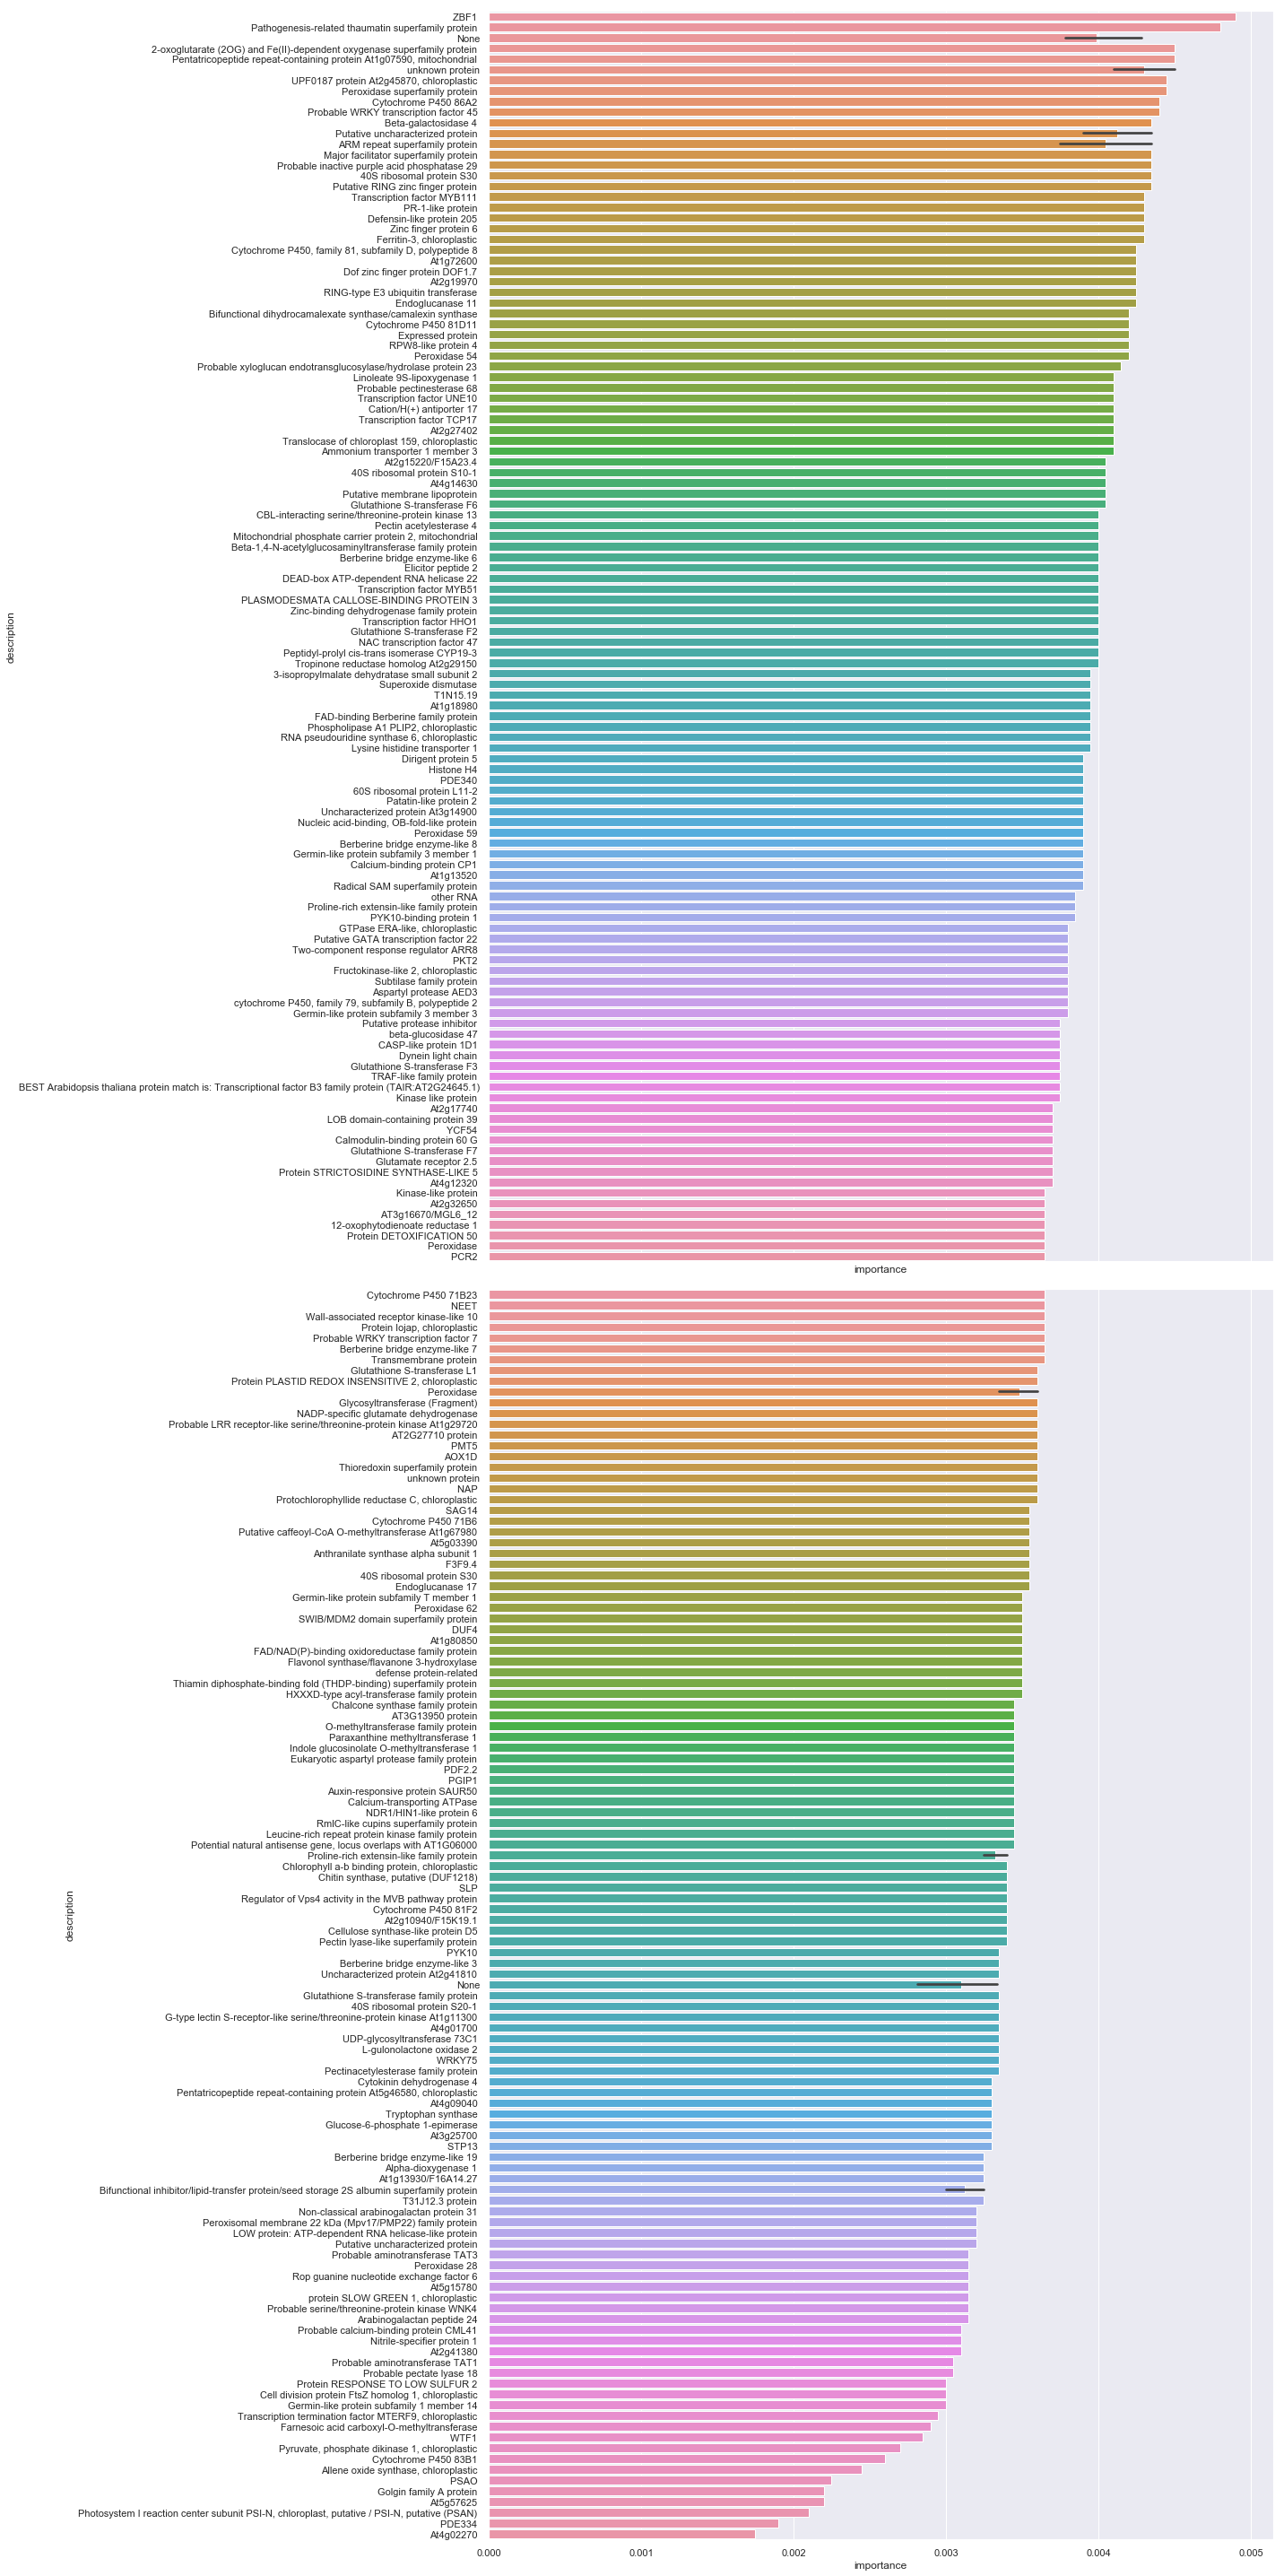
\includegraphics[width=.9\linewidth]{obipy-resources/93e2fbf76ed477962282ae99767b8408de4d3ed9/69bf10916878bd9338319e6d6934a10bcca2934b.png}
\end{center}

\section{Selecting genes for Lym2 at 6hr C/W}
\label{sec:org1a7bf55}
\subsection{RFE selecting 25 genes}
\label{sec:orgf2dd900}
\begin{minted}[frame=lines,linenos=true,fontfamily=Monaco]{ipython}
from sklearn.feature_selection import RFE, RFECV
from sklearn.linear_model import LogisticRegression

# load data
DE_pairings_6hr = read_xl('/Users/hughesn/PHD/Transcripts/Data/pairings_6hr.xlsx')
sig = DE_pairings_05hr[DE_pairings_05hr['padj'] < 0.05]
sig = sig['log2FoldChange'].sort_values()
locs = sig.index
df = counts.loc[locs][[c for c in counts.columns if ('6h' in c and 'lym' in c)]].T
df = df.loc[:,~df.columns.duplicated()]
df = df[[c for c in set(df.columns.values)]]
\end{minted}

\begin{minted}[frame=lines,linenos=true,fontfamily=Monaco]{ipython}
# Feature Extraction with RFE
X = df.values
y = [y.rsplit('_',1)[0] for y in df.reset_index()['index']]
# feature extraction
model = LogisticRegression()
rfe = RFE(model, n_features_to_select=25)
fit = rfe.fit(X, y)
print("Num Features: {0}".format(fit.n_features_))
print("Selected Features: {0}".format(fit.support_))
print("Feature Ranking: {0}".format(fit.ranking_))
\end{minted}

Num Features: 25\\
Selected Features: [False False False \ldots{} False False False]\\
Feature Ranking: [  54 2703 2480 \ldots{} 3084 4681 4184]\\


\begin{minted}[frame=lines,linenos=true,fontfamily=Monaco]{ipython}
genes = []
for r,f in zip(fit.ranking_, df.columns.values):
      if r ==1:
            genes.append(f)
get_gene_names(genes)
\end{minted}

\begin{center}
\begin{tabular}{rlll}
 & incoming & name & description\\
\hline
0 & AT1G18970 & GLP1 & Germin-like protein subfamily T member 1\\
1 & AT3G16420 & PBP1 & PYK10-binding protein 1\\
2 & AT2G19970 & AT2G19970 & At2g19970\\
3 & AT3G09260 & BGLU23 & PYK10\\
4 & AT3G28740 & CYP81D11 & Cytochrome P450 81D11\\
5 & AT2G15220 & AT2G15220 & At2g15220/F15A23.4\\
6 & AT3G01420 & DOX1 & Alpha-dioxygenase 1\\
7 & AT1G02930 & GSTF6 & Glutathione S-transferase F6\\
8 & AT4G25220 & RHS15 & Putative glycerol-3-phosphate transporter 2\\
9 & AT5G14330 & AT5G14330 & Transmembrane protein\\
10 & AT2G26560 & PLP2 & Patatin-like protein 2\\
11 & AT1G26240 & AT1G26240 & Proline-rich extensin-like family protein\\
12 & AT2G38870 & AT2G38870 & Putative protease inhibitor\\
13 & AT1G09310 & AT1G09310 & T31J12.3 protein\\
14 & AT1G26380 & FOX1 & Berberine bridge enzyme-like 3\\
15 & AT1G02920 & GSTF7 & Glutathione S-transferase F7\\
16 & AT3G16400 & NSP1 & Nitrile-specifier protein 1\\
17 & AT2G27402 & AT2G27402 & At2g27402\\
18 & AT5G20630 & GER3 & Germin-like protein subfamily 3 member 3\\
19 & AT1G66700 & PXMT1 & Paraxanthine methyltransferase 1\\
20 & AT5G08640 & FLS1 & Flavonol synthase/flavanone 3-hydroxylase\\
21 & AT5G13930 & CHS & Chalcone synthase family protein\\
22 & AT1G21120 & AT1G21120 & O-methyltransferase family protein\\
23 & AT5G47500 & PME68 & Probable pectinesterase 68\\
24 & AT5G39110 & AT5G39110 & Germin-like protein subfamily 1 member 14\\
\end{tabular}
\end{center}


\subsubsection{Forest on this RFE set}
\label{sec:orge7324dc}

\begin{minted}[frame=lines,linenos=true,fontfamily=Monaco]{ipython}
rfe_forest = counts.loc[genes][[c for c in counts.columns if ('6h' in c and 'lym' in c)]].T
rfe_forest = rfe_forest.loc[:,~rfe_forest.columns.duplicated()]
rfe_forest = rfe_forest[[c for c in set(rfe_forest.columns.values)]]

feat_labels = rfe_forest.columns.values
y = [d.rsplit('_', 1)[0] for d in rfe_forest.index.values]

X_train, X_test, y_train, y_test = train_test_split(rfe_forest.values, y, test_size=1, random_state=42)
forest = RandomForestClassifier(n_estimators=20000, random_state=1, n_jobs=-1)
forest.fit(X_train, y_train)
res = {k: v for k, v in sorted(
    zip(feat_labels, forest.feature_importances_), key=lambda x: x[1], reverse=True)}
res_df = pd.DataFrame(list(res.items()), columns=[
                      'gene', 'importance']).set_index('gene')
names = get_gene_names(list(res_df.index))
res_df = pd.merge(res_df, names, left_index=True, right_on='incoming').rename(
    columns={'incoming': 'gene'}).set_index('gene').sort_values('importance', ascending=False)
res_df
\end{minted}

\begin{center}
\begin{tabular}{lrll}
gene & importance & name & description\\
\hline
AT4G25220 & 0.03965 & RHS15 & Putative glycerol-3-phosphate transporter 2\\
AT1G02930 & 0.039 & GSTF6 & Glutathione S-transferase F6\\
AT3G09260 & 0.03815 & BGLU23 & PYK10\\
AT2G19970 & 0.03755 & AT2G19970 & At2g19970\\
AT1G21120 & 0.0375 & AT1G21120 & O-methyltransferase family protein\\
AT3G28740 & 0.03745 & CYP81D11 & Cytochrome P450 81D11\\
AT2G15220 & 0.03725 & AT2G15220 & At2g15220/F15A23.4\\
AT1G18970 & 0.03705 & GLP1 & Germin-like protein subfamily T member 1\\
AT5G20630 & 0.037 & GER3 & Germin-like protein subfamily 3 member 3\\
AT5G13930 & 0.0369 & CHS & Chalcone synthase family protein\\
AT3G16400 & 0.03675 & NSP1 & Nitrile-specifier protein 1\\
AT1G26380 & 0.0366 & FOX1 & Berberine bridge enzyme-like 3\\
AT3G16420 & 0.03635 & PBP1 & PYK10-binding protein 1\\
AT1G66700 & 0.03625 & PXMT1 & Paraxanthine methyltransferase 1\\
AT1G09310 & 0.0362 & AT1G09310 & T31J12.3 protein\\
AT1G02920 & 0.0362 & GSTF7 & Glutathione S-transferase F7\\
AT2G27402 & 0.0361 & AT2G27402 & At2g27402\\
AT1G26240 & 0.03585 & AT1G26240 & Proline-rich extensin-like family protein\\
AT2G38870 & 0.0358 & AT2G38870 & Putative protease inhibitor\\
AT5G47500 & 0.0356 & PME68 & Probable pectinesterase 68\\
AT5G39110 & 0.03545 & AT5G39110 & Germin-like protein subfamily 1 member 14\\
AT2G26560 & 0.035 & PLP2 & Patatin-like protein 2\\
AT5G14330 & 0.03495 & AT5G14330 & Transmembrane protein\\
AT3G01420 & 0.03425 & DOX1 & Alpha-dioxygenase 1\\
AT5G08640 & 0.0341 & FLS1 & Flavonol synthase/flavanone 3-hydroxylase\\
\end{tabular}
\end{center}

\begin{minted}[frame=lines,linenos=true,fontfamily=Monaco]{ipython}
fig, ax = plt.subplots(1, figsize=(20,20))
sns.barplot(data=res_df.reset_index(), y='description', x='importance')
plt.tight_layout()
\end{minted}

\begin{verbatim}
<Figure size 1440x1440 with 1 Axes>
\end{verbatim}


\begin{center}
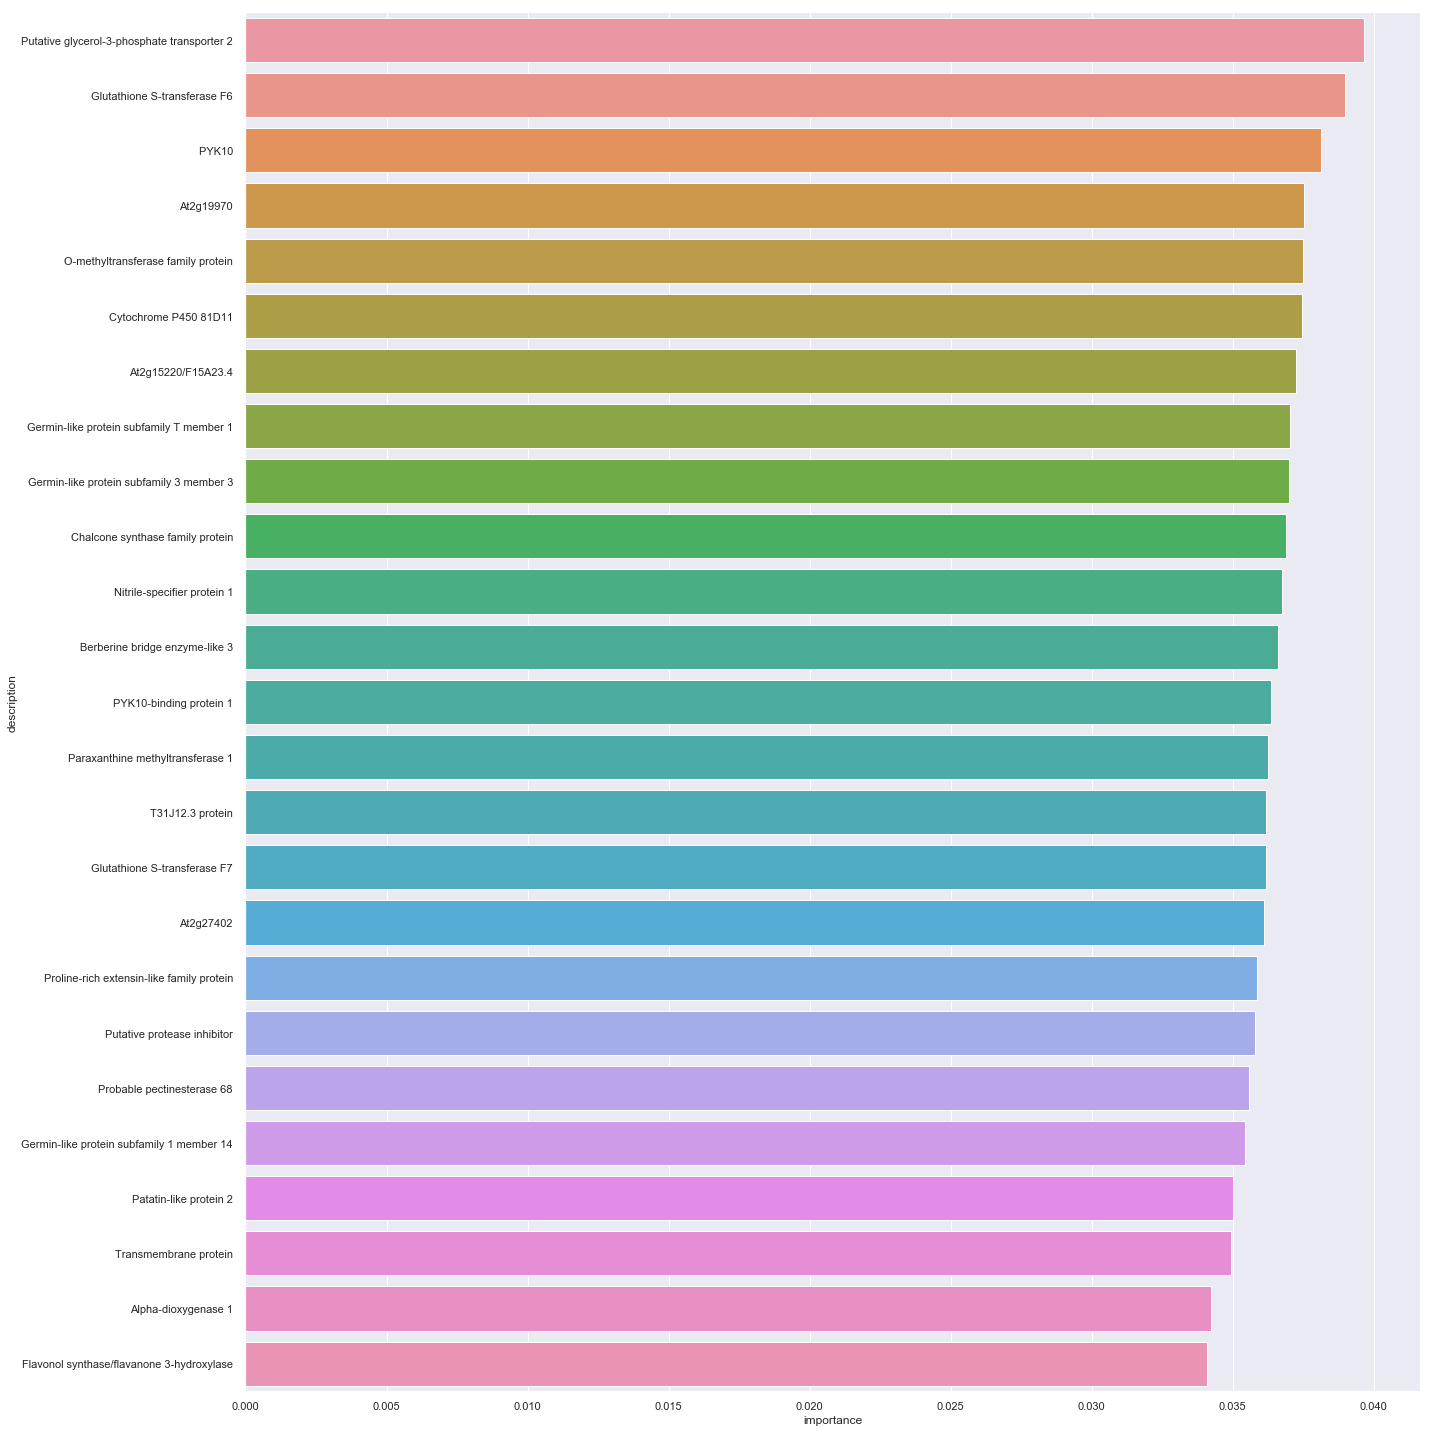
\includegraphics[width=.9\linewidth]{obipy-resources/93e2fbf76ed477962282ae99767b8408de4d3ed9/21f33ed725c0b0940b60e1588a12604820f36aa7.png}
\end{center}


\subsection{RFE selecting 250 genes}
\label{sec:org2f8fc04}
\begin{minted}[frame=lines,linenos=true,fontfamily=Monaco]{ipython}
from sklearn.feature_selection import RFE, RFECV
from sklearn.linear_model import LogisticRegression

# load data
DE_pairings_6hr = read_xl('/Users/hughesn/PHD/Transcripts/Data/pairings_6hr.xlsx')
sig = DE_pairings_05hr[DE_pairings_05hr['padj'] < 0.05]
sig = sig['log2FoldChange'].sort_values()
locs = sig.index
df = counts.loc[locs][[c for c in counts.columns if ('6h' in c and 'col' in c)]].T
df = df.loc[:,~df.columns.duplicated()]
df = df[[c for c in set(df.columns.values)]]
\end{minted}

\begin{minted}[frame=lines,linenos=true,fontfamily=Monaco]{ipython}
# Feature Extraction with RFE
X = df.values
y = [y.rsplit('_',1)[0] for y in df.reset_index()['index']]
# feature extraction
model = LogisticRegression()
rfe = RFE(model, n_features_to_select=250)
fit = rfe.fit(X, y)
print("Num Features: {0}".format(fit.n_features_))
print("Selected Features: {0}".format(fit.support_))
print("Feature Ranking: {0}".format(fit.ranking_))
\end{minted}

Num Features: 250\\
Selected Features: [ True False False \ldots{} False False False]\\
Feature Ranking: [   1 1670 4977 \ldots{}  582  748 4096]\\


\begin{minted}[frame=lines,linenos=true,fontfamily=Monaco]{ipython}
genes = []
for r,f in zip(fit.ranking_, df.columns.values):
      if r ==1:
            genes.append(f)
get_gene_names(genes)
\end{minted}



\begin{center}
\begin{tabular}{rlll}
 & incoming & name & description\\
\hline
0 & AT1G59990 & RH22 & DEAD-box ATP-dependent RNA helicase 22\\
1 & AT1G18970 & GLP1 & Germin-like protein subfamily T member 1\\
2 & AT4G26010 & AT4G26010 & Peroxidase superfamily protein\\
3 & AT1G06002 & AT1G06002 & Potential natural antisense gene, locus overlaps with AT1G06000\\
4 & AT3G01970 & WRKY45 & Probable WRKY transcription factor 45\\
5 & AT5G05735 & AT5G05735 & None\\
6 & AT4G20830 & AT4G20830 & Berberine bridge enzyme-like 19\\
7 & AT5G06865 & AT5G06865 & other RNA\\
8 & AT3G16420 & PBP1 & PYK10-binding protein 1\\
9 & AT4G29390 & RPS30A & 40S ribosomal protein S30\\
10 & AT5G24660 & LSU2 & Protein RESPONSE TO LOW SULFUR 2\\
11 & AT5G58350 & WNK4 & Probable serine/threonine-protein kinase WNK4\\
12 & AT2G24180 & CYP71B6 & Cytochrome P450 71B6\\
13 & AT4G39950 & CYP79B2 & cytochrome P450, family 79, subfamily B, polypeptide 2\\
14 & AT5G19890 & PER59 & Peroxidase 59\\
15 & AT2G10940 & AT2G10940 & At2g10940/F15K19.1\\
16 & AT2G36750 & UGT73C1 & UDP-glycosyltransferase 73C1\\
17 & AT3G04070 & NAC047 & NAC transcription factor 47\\
18 & AT3G21305 & AT3G21305 & None\\
19 & AT3G25700 & AT3G25700 & At3g25700\\
20 & AT2G19970 & AT2G19970 & At2g19970\\
21 & AT1G30530 & UGT78D1 & Glycosyltransferase (Fragment)\\
22 & AT1G76680 & OPR1 & 12-oxophytodienoate reductase 1\\
23 & AT1G18975 & AT1G18975 & None\\
24 & AT3G09260 & BGLU23 & PYK10\\
25 & AT5G57220 & CYP81F2 & Cytochrome P450 81F2\\
26 & AT1G18650 & PDCB3 & PLASMODESMATA CALLOSE-BINDING PROTEIN 3\\
27 & AT5G49480 & ATCP1 & Calcium-binding protein CP1\\
28 & AT4G23700 & CHX17 & Cation/H(+) antiporter 17\\
29 & AT5G64120 & PER71 & Peroxidase\\
30 & AT5G64890 & PEP2 & Elicitor peptide 2\\
31 & AT3G03670 & PER28 & Peroxidase 28\\
32 & AT1G15885 & AT1G15885 & Putative uncharacterized protein\\
33 & AT3G18830 & PLT5 & PMT5\\
34 & AT3G28740 & CYP81D11 & Cytochrome P450 81D11\\
35 & AT3G50480 & HR4 & RPW8-like protein 4\\
36 & AT1G79680 & WAKL10 & Wall-associated receptor kinase-like 10\\
37 & AT1G09750 & AED3 & Aspartyl protease AED3\\
38 & AT2G15220 & AT2G15220 & At2g15220/F15A23.4\\
39 & AT4G02290 & AtGH9B13 & Endoglucanase 17\\
40 & AT1G03220 & AT1G03220 & Eukaryotic aspartyl protease family protein\\
41 & AT1G26410 & FOX4 & Berberine bridge enzyme-like 6\\
42 & AT4G34760 & SAUR50 & Auxin-responsive protein SAUR50\\
43 & AT5G38900 & AT5G38900 & Thioredoxin superfamily protein\\
44 & AT1G14540 & PER4 & Peroxidase\\
45 & AT3G01420 & DOX1 & Alpha-dioxygenase 1\\
46 & AT3G55660 & ROPGEF6 & Rop guanine nucleotide exchange factor 6\\
47 & AT3G51430 & SSL5 & Protein STRICTOSIDINE SYNTHASE-LIKE 5\\
48 & AT1G02930 & GSTF6 & Glutathione S-transferase F6\\
49 & AT2G41810 & AT2G41810 & Uncharacterized protein At2g41810\\
50 & AT1G28290 & AGP31 & Non-classical arabinogalactan protein 31\\
51 & AT4G19420 & AT4G19420 & Pectinacetylesterase family protein\\
52 & AT5G44380 & AT5G44380 & FAD-binding Berberine family protein\\
53 & AT1G26250 & AT1G26250 & Proline-rich extensin-like family protein\\
54 & AT1G02730 & CSLD5 & Cellulose synthase-like protein D5\\
55 & AT4G30720 & AT4G30720 & FAD/NAD(P)-binding oxidoreductase family protein\\
56 & AT2G36690 & AT2G36690 & 2-oxoglutarate (2OG) and Fe(II)-dependent oxygenase superfamily protein\\
57 & AT1G62510 & AT1G62510 & Bifunctional inhibitor/lipid-transfer protein/seed storage 2S albumin superfamily protein\\
58 & AT5G46580 & AT5G46580 & Pentatricopeptide repeat-containing protein At5g46580, chloroplastic\\
59 & AT1G15260 & AT1G15260 & LOW protein: ATP-dependent RNA helicase-like protein\\
60 & AT1G21100 & IGMT1 & Indole glucosinolate O-methyltransferase 1\\
61 & AT4G34950 & AT4G34950 & Major facilitator superfamily protein\\
62 & AT3G09405 & PAE4 & Pectin acetylesterase 4\\
63 & AT5G03390 & AT5G03390 & At5g03390\\
64 & AT2G43120 & AT2G43120 & RmlC-like cupins superfamily protein\\
65 & AT1G21400 & AT1G21400 & Thiamin diphosphate-binding fold (THDP-binding) superfamily protein\\
66 & AT5G42830 & AT5G42830 & HXXXD-type acyl-transferase family protein\\
67 & AT1G67148 & AT1G67148 & Putative uncharacterized protein\\
68 & AT5G52050 & DTX50 & Protein DETOXIFICATION 50\\
69 & AT3G06145 & AT3G06145 & Putative RING zinc finger protein\\
70 & AT3G26210 & CYP71B23 & Cytochrome P450 71B23\\
71 & AT1G65490 & AT1G65490 & unknown protein\\
72 & AT5G48880 & KAT5 & PKT2\\
73 & AT4G25810 & XTH23 & Probable xyloglucan endotransglucosylase/hydrolase protein 23\\
74 & AT2G27389 & AT2G27389 & unknown protein\\
75 & AT5G67400 & PER73 & Peroxidase\\
76 & AT5G55580 & MTERF9 & Transcription termination factor MTERF9, chloroplastic\\
77 & AT5G05730 & ASA1 & Anthranilate synthase alpha subunit 1\\
78 & AT5G26340 & STP13 & STP13\\
79 & AT4G21760 & BGLU47 & beta-glucosidase 47\\
80 & AT1G48570 & AT1G48570 & T1N15.19\\
81 & AT5G54810 & TSB1 & Tryptophan synthase\\
82 & AT1G67980 & CCOAMT & Putative caffeoyl-CoA O-methyltransferase At1g67980\\
83 & AT5G14330 & AT5G14330 & Transmembrane protein\\
84 & AT4G19370 & AT4G19370 & Chitin synthase, putative (DUF1218)\\
85 & AT5G13080 & WRKY75 & WRKY75\\
86 & AT1G03630 & PORC & Protochlorophyllide reductase C, chloroplastic\\
87 & AT2G27710 & RPP2B & AT2G27710 protein\\
88 & AT4G21770 & AT4G21770 & RNA pseudouridine synthase 6, chloroplastic\\
89 & AT1G69490 & NAC029 & NAP\\
90 & AT5G39580 & PER62 & Peroxidase 62\\
91 & AT3G54580 & AT3G54580 & Proline-rich extensin-like family protein\\
92 & AT5G11550 & AT5G11550 & ARM repeat superfamily protein\\
93 & AT4G15610 & AT4G15610 & CASP-like protein 1D1\\
94 & AT1G64160 & DIR5 & Dirigent protein 5\\
95 & AT5G49330 & MYB111 & Transcription factor MYB111\\
96 & AT3G48850 & MPT2 & Mitochondrial phosphate carrier protein 2, mitochondrial\\
97 & AT4G37540 & LBD39 & LOB domain-containing protein 39\\
98 & AT2G26560 & PLP2 & Patatin-like protein 2\\
99 & AT5G58250 & AT5G58250 & YCF54\\
100 & AT4G01037 & WTF1 & WTF1\\
101 & AT3G48500 & PDE312 & Nucleic acid-binding, OB-fold-like protein\\
102 & AT3G13950 & AT3G13950 & AT3G13950 protein\\
103 & AT4G09040 & AT4G09040 & At4g09040\\
104 & AT2G19990 & PR-1-LIKE & PR-1-like protein\\
105 & AT2G12170 & AT2G12170 & BEST Arabidopsis thaliana protein match is: Transcriptional factor B3 family protein (TAIR:AT2G24645.1)\\
106 & AT5G14650 & AT5G14650 & Pectin lyase-like superfamily protein\\
107 & AT3G52450 & PUB22 & RING-type E3 ubiquitin transferase\\
108 & AT5G56670 & RPS30A & 40S ribosomal protein S30\\
109 & AT1G26240 & AT1G26240 & Proline-rich extensin-like family protein\\
110 & AT3G63380 & ACA12 & Calcium-transporting ATPase\\
111 & AT2G38870 & AT2G38870 & Putative protease inhibitor\\
112 & AT5G23310 & FSD3 & Superoxide dismutase\\
113 & AT4G24780 & AT4G24780 & Probable pectate lyase 18\\
114 & AT1G10522 & PRIN2 & Protein PLASTID REDOX INSENSITIVE 2, chloroplastic\\
115 & AT3G14900 & AT3G14900 & Uncharacterized protein At3g14900\\
116 & AT4G28420 & AT4G28420 & Probable aminotransferase TAT1\\
117 & AT2G24850 & TAT3 & Probable aminotransferase TAT3\\
118 & AT2G46840 & DUF4 & DUF4\\
119 & AT4G02520 & GSTF2 & Glutathione S-transferase F2\\
120 & AT1G09310 & AT1G09310 & T31J12.3 protein\\
121 & AT4G35730 & AT4G35730 & Regulator of Vps4 activity in the MVB pathway protein\\
122 & AT1G51700 & DOF1.7 & Dof zinc finger protein DOF1.7\\
123 & AT1G05523 & AT1G05523 & None\\
124 & AT3G24300 & AMT1-3 & Ammonium transporter 1 member 3\\
125 & AT4G14630 & GLP9 & At4g14630\\
126 & AT4G00050 & UNE10 & Transcription factor UNE10\\
127 & AT1G26380 & FOX1 & Berberine bridge enzyme-like 3\\
128 & AT1G02920 & GSTF7 & Glutathione S-transferase F7\\
129 & AT5G15780 & AT5G15780 & At5g15780\\
130 & AT3G25790 & HHO1 & Transcription factor HHO1\\
131 & AT3G18420 & SG1 & protein SLOW GREEN 1, chloroplastic\\
132 & AT4G02510 & TOC159 & Translocase of chloroplast 159, chloroplastic\\
133 & AT4G18730 & RPL11C & 60S ribosomal protein L11-2\\
134 & AT3G58990 & IPMI1 & 3-isopropylmalate dehydratase small subunit 2\\
135 & AT5G02780 & GSTL1 & Glutathione S-transferase L1\\
136 & AT1G13930 & AT1G13930 & At1g13930/F16A14.27\\
137 & AT1G69200 & FLN2 & Fructokinase-like 2, chloroplastic\\
138 & AT4G25740 & RPS10A & 40S ribosomal protein S10-1\\
139 & AT5G55280 & FTSZ1 & Cell division protein FtsZ homolog 1, chloroplastic\\
140 & AT1G29720 & RFK1 & Probable LRR receptor-like serine/threonine-protein kinase At1g29720\\
141 & AT5G40780 & LHT1 & Lysine histidine transporter 1\\
142 & AT5G66530 & AT5G66530 & Glucose-6-phosphate 1-epimerase\\
143 & AT5G06860 & PGIP1 & PGIP1\\
144 & AT3G16400 & NSP1 & Nitrile-specifier protein 1\\
145 & AT3G56090 & FER3 & Ferritin-3, chloroplastic\\
146 & AT2G27402 & AT2G27402 & At2g27402\\
147 & AT5G40730 & AGP24 & Arabinogalactan peptide 24\\
148 & AT5G20230 & BCB & SAG14\\
149 & AT1G30700 & AT1G30700 & Berberine bridge enzyme-like 8\\
150 & AT5G20790 & AT5G20790 & unknown protein\\
151 & AT3G62530 & AT3G62530 & ARM repeat superfamily protein\\
152 & AT2G17740 & AT2G17740 & At2g17740\\
153 & AT2G41310 & ARR8 & Two-component response regulator ARR8\\
154 & AT4G37370 & CYP81D8 & Cytochrome P450, family 81, subfamily D, polypeptide 8\\
155 & AT5G51720 & NEET & NEET\\
156 & AT1G55020 & LOX1 & Linoleate 9S-lipoxygenase 1\\
157 & AT1G08757 & AT1G08757 & None\\
158 & AT1G52245 & AT1G52245 & Dynein light chain\\
159 & AT1G71695 & PER12 & Peroxidase\\
160 & AT5G44990 & AT5G44990 & Glutathione S-transferase family protein\\
161 & AT3G45030 & RPS20C & 40S ribosomal protein S20-1\\
162 & AT1G65690 & NHL6 & NDR1/HIN1-like protein 6\\
163 & AT1G26255 & AT1G26255 & None\\
164 & AT4G02270 & RHS13 & At4g02270\\
165 & AT4G00360 & CYP86A2 & Cytochrome P450 86A2\\
166 & AT2G02100 & PDF2.2 & PDF2.2\\
167 & AT3G50770 & CML41 & Probable calcium-binding protein CML41\\
168 & AT4G26150 & GATA22 & Putative GATA transcription factor 22\\
169 & AT2G29150 & AT2G29150 & Tropinone reductase homolog At2g29150\\
170 & AT2G32990 & AtGH9B8 & Endoglucanase 11\\
171 & AT5G20630 & GER3 & Germin-like protein subfamily 3 member 3\\
172 & AT5G08610 & RH26 & PDE340\\
173 & AT3G05730 & AT3G05730 & Defensin-like protein 205\\
174 & AT3G44860 & FAMT & Farnesoic acid carboxyl-O-methyltransferase\\
175 & AT1G13520 & AT1G13520 & At1g13520\\
176 & AT1G08380 & PSAO & PSAO\\
177 & AT5G63140 & PAP29 & Probable inactive purple acid phosphatase 29\\
178 & AT5G66470 & AT5G66470 & GTPase ERA-like, chloroplastic\\
179 & AT1G02660 & PLIP2 & Phospholipase A1 PLIP2, chloroplastic\\
180 & AT1G78450 & AT1G78450 & F3F9.4\\
181 & AT5G19750 & AT5G19750 & Peroxisomal membrane 22 kDa (Mpv17/PMP22) family protein\\
182 & AT5G64040 & PSAN & Photosystem I reaction center subunit PSI-N, chloroplast, putative / PSI-N, putative (PSAN)\\
183 & AT4G29740 & CKX4 & Cytokinin dehydrogenase 4\\
184 & AT1G18250 & ATLP-1 & Pathogenesis-related thaumatin superfamily protein\\
185 & AT3G18250 & AT3G18250 & Putative membrane lipoprotein\\
186 & AT3G16670 & AT3G16670 & AT3g16670/MGL6\_12\\
187 & AT1G18980 & AT1G18980 & At1g18980\\
188 & AT4G34290 & AT4G34290 & SWIB/MDM2 domain superfamily protein\\
189 & AT3G46280 & AT3G46280 & Kinase-like protein\\
190 & AT4G20835 & AT4G20835 & None\\
191 & AT1G66700 & PXMT1 & Paraxanthine methyltransferase 1\\
192 & AT3G26445 & AT3G26445 & Beta-1,4-N-acetylglucosaminyltransferase family protein\\
193 & AT5G26920 & CBP60G & Calmodulin-binding protein 60 G\\
194 & AT5G16980 & AT5G16980 & Zinc-binding dehydrogenase family protein\\
195 & AT4G10530 & AT4G10530 & Subtilase family protein\\
196 & AT3G54890 & LHCA1 & Chlorophyll a-b binding protein, chloroplastic\\
197 & AT2G28000 & CPN60A1 & SLP\\
198 & AT4G24240 & WRKY7 & Probable WRKY transcription factor 7\\
199 & AT2G41380 & AT2G41380 & At2g41380\\
200 & AT1G18570 & MYB51 & Transcription factor MYB51\\
201 & AT3G56070 & CYP19-3 & Peptidyl-prolyl cis-trans isomerase CYP19-3\\
202 & AT5G08640 & FLS1 & Flavonol synthase/flavanone 3-hydroxylase\\
203 & AT1G06000 & UGT89C1 & Glycosyltransferase (Fragment)\\
204 & AT4G30090 & AT4G30090 & Golgin family A protein\\
205 & AT5G56870 & BGAL4 & Beta-galactosidase 4\\
206 & AT5G42650 & CYP74A & Allene oxide synthase, chloroplastic\\
207 & AT4G29905 & AT4G29905 & Putative uncharacterized protein\\
208 & AT2G46750 & GULLO2 & L-gulonolactone oxidase 2\\
209 & AT5G13930 & CHS & Chalcone synthase family protein\\
210 & AT3G26830 & CYP71B15 & Bifunctional dihydrocamalexate synthase/camalexin synthase\\
211 & AT2G45870 & AT2G45870 & UPF0187 protein At2g45870, chloroplastic\\
212 & AT1G32640 & MYC2 & ZBF1\\
213 & AT4G03985 & AT4G03985 & None\\
214 & AT4G12320 & CYP706A6 & At4g12320\\
215 & AT2G28740 & HIS4 & Histone H4\\
216 & AT2G25297 & AT2G25297 & None\\
217 & AT5G06730 & PER54 & Peroxidase 54\\
218 & AT1G26420 & FOX5 & Berberine bridge enzyme-like 7\\
219 & AT5G48657 & AT5G48657 & defense protein-related\\
220 & AT1G11300 & AT1G11300 & G-type lectin S-receptor-like serine/threonine-protein kinase At1g11300\\
221 & AT4G32260 & AT4G32260 & PDE334\\
222 & AT2G32650 & AT2G32650 & At2g32650\\
223 & AT1G21120 & AT1G21120 & O-methyltransferase family protein\\
224 & AT1G72600 & AT1G72600 & At1g72600\\
225 & AT5G08070 & TCP17 & Transcription factor TCP17\\
226 & AT5G57625 & AT5G57625 & At5g57625\\
227 & AT1G67030 & ZFP6 & Zinc finger protein 6\\
228 & AT1G72610 & GLP1 & Germin-like protein subfamily 3 member 1\\
229 & AT2G02930 & GSTF3 & Glutathione S-transferase F3\\
230 & AT5G47500 & PME68 & Probable pectinesterase 68\\
231 & AT5G07030 & AT5G07030 & Eukaryotic aspartyl protease family protein\\
232 & AT1G80850 & AT1G80850 & At1g80850\\
233 & AT1G51890 & AT1G51890 & Leucine-rich repeat protein kinase family protein\\
234 & AT2G18690 & AT2G18690 & Expressed protein\\
235 & AT2G48130 & AT2G48130 & Bifunctional inhibitor/lipid-transfer protein/seed storage 2S albumin superfamily protein\\
236 & AT4G14780 & AT4G14780 & Kinase like protein\\
237 & AT2G34180 & CIPK13 & CBL-interacting serine/threonine-protein kinase 13\\
238 & AT4G15530 & PPDK & Pyruvate, phosphate dikinase 1, chloroplastic\\
239 & AT1G32350 & AOX3 & AOX1D\\
240 & AT1G07590 & AT1G07590 & Pentatricopeptide repeat-containing protein At1g07590, mitochondrial\\
241 & AT5G26290 & AT5G26290 & TRAF-like family protein\\
242 & AT5G11210 & GLR2.5 & Glutamate receptor 2.5\\
243 & AT4G24110 & AT4G24110 & NADP-specific glutamate dehydrogenase\\
244 & AT4G01700 & AT4G01700 & At4g01700\\
245 & AT4G31500 & CYP83B1 & Cytochrome P450 83B1\\
246 & AT1G14870 & PCR2 & PCR2\\
247 & AT2G39670 & AT2G39670 & Radical SAM superfamily protein\\
248 & AT3G12930 & IJ & Protein Iojap, chloroplastic\\
249 & AT5G39110 & AT5G39110 & Germin-like protein subfamily 1 member 14\\
\end{tabular}
\end{center}


\paragraph{Forest on this RFE}
\label{sec:org38e734e}

\begin{minted}[frame=lines,linenos=true,fontfamily=Monaco]{ipython}
rfe_forest = counts.loc[genes][[c for c in counts.columns if ('6h' in c and 'lym' in c)]].T
rfe_forest = rfe_forest.loc[:,~rfe_forest.columns.duplicated()]
rfe_forest = rfe_forest[[c for c in set(rfe_forest.columns.values)]]

feat_labels = rfe_forest.columns.values
y = [d.rsplit('_', 1)[0] for d in rfe_forest.index.values]

X_train, X_test, y_train, y_test = train_test_split(rfe_forest.values, y, test_size=1, random_state=42)
forest = RandomForestClassifier(n_estimators=20000, random_state=1, n_jobs=-1)
forest.fit(X_train, y_train)
res = {k: v for k, v in sorted(
    zip(feat_labels, forest.feature_importances_), key=lambda x: x[1], reverse=True)}
res_df = pd.DataFrame(list(res.items()), columns=[
                      'gene', 'importance']).set_index('gene')
names = get_gene_names(list(res_df.index))
res_df = pd.merge(res_df, names, left_index=True, right_on='incoming').rename(
    columns={'incoming': 'gene'}).set_index('gene').sort_values('importance', ascending=False)
res_df
\end{minted}

\begin{center}
\begin{tabular}{lrll}
gene & importance & name & description\\
\hline
AT1G18250 & 0.0052 & ATLP-1 & Pathogenesis-related thaumatin superfamily protein\\
AT2G27389 & 0.0052 & AT2G27389 & unknown protein\\
AT4G26010 & 0.0051 & AT4G26010 & Peroxidase superfamily protein\\
AT2G45870 & 0.005 & AT2G45870 & UPF0187 protein At2g45870, chloroplastic\\
AT4G00360 & 0.005 & CYP86A2 & Cytochrome P450 86A2\\
AT2G36690 & 0.005 & AT2G36690 & 2-oxoglutarate (2OG) and Fe(II)-dependent oxygenase superfamily protein\\
AT5G49330 & 0.00495 & MYB111 & Transcription factor MYB111\\
AT1G67148 & 0.0049 & AT1G67148 & Putative uncharacterized protein\\
AT4G03985 & 0.0049 & AT4G03985 & None\\
AT3G26830 & 0.00485 & CYP71B15 & Bifunctional dihydrocamalexate synthase/camalexin synthase\\
AT4G23700 & 0.00485 & CHX17 & Cation/H(+) antiporter 17\\
AT3G06145 & 0.00485 & AT3G06145 & Putative RING zinc finger protein\\
AT4G34950 & 0.00485 & AT4G34950 & Major facilitator superfamily protein\\
AT3G01970 & 0.00485 & WRKY45 & Probable WRKY transcription factor 45\\
AT1G55020 & 0.0048 & LOX1 & Linoleate 9S-lipoxygenase 1\\
AT5G40780 & 0.0048 & LHT1 & Lysine histidine transporter 1\\
AT2G19990 & 0.00475 & PR-1-LIKE & PR-1-like protein\\
AT5G63140 & 0.00475 & PAP29 & Probable inactive purple acid phosphatase 29\\
AT3G50480 & 0.00475 & HR4 & RPW8-like protein 4\\
AT4G02520 & 0.00475 & GSTF2 & Glutathione S-transferase F2\\
AT4G02510 & 0.00475 & TOC159 & Translocase of chloroplast 159, chloroplastic\\
AT5G47500 & 0.0047 & PME68 & Probable pectinesterase 68\\
AT2G38870 & 0.0047 & AT2G38870 & Putative protease inhibitor\\
AT4G37370 & 0.0047 & CYP81D8 & Cytochrome P450, family 81, subfamily D, polypeptide 8\\
AT1G64160 & 0.0047 & DIR5 & Dirigent protein 5\\
AT2G26560 & 0.0047 & PLP2 & Patatin-like protein 2\\
AT3G52450 & 0.0047 & PUB22 & RING-type E3 ubiquitin transferase\\
AT3G56090 & 0.0047 & FER3 & Ferritin-3, chloroplastic\\
AT5G66470 & 0.00465 & AT5G66470 & GTPase ERA-like, chloroplastic\\
AT2G29150 & 0.00465 & AT2G29150 & Tropinone reductase homolog At2g29150\\
AT3G28740 & 0.00465 & CYP81D11 & Cytochrome P450 81D11\\
AT2G25297 & 0.00465 & AT2G25297 & None\\
AT2G15220 & 0.0046 & AT2G15220 & At2g15220/F15A23.4\\
AT1G48570 & 0.0046 & AT1G48570 & T1N15.19\\
AT3G04070 & 0.0046 & NAC047 & NAC transcription factor 47\\
AT1G18650 & 0.0046 & PDCB3 & PLASMODESMATA CALLOSE-BINDING PROTEIN 3\\
AT5G06730 & 0.0046 & PER54 & Peroxidase 54\\
AT1G79680 & 0.0046 & WAKL10 & Wall-associated receptor kinase-like 10\\
AT2G19970 & 0.0046 & AT2G19970 & At2g19970\\
AT3G48500 & 0.0046 & PDE312 & Nucleic acid-binding, OB-fold-like protein\\
AT4G26150 & 0.00455 & GATA22 & Putative GATA transcription factor 22\\
AT4G14630 & 0.00455 & GLP9 & At4g14630\\
AT4G10530 & 0.00455 & AT4G10530 & Subtilase family protein\\
AT3G05730 & 0.00455 & AT3G05730 & Defensin-like protein 205\\
AT4G21770 & 0.00455 & AT4G21770 & RNA pseudouridine synthase 6, chloroplastic\\
AT3G14900 & 0.00455 & AT3G14900 & Uncharacterized protein At3g14900\\
AT4G14780 & 0.00455 & AT4G14780 & Kinase like protein\\
AT2G18690 & 0.00455 & AT2G18690 & Expressed protein\\
AT2G27402 & 0.00455 & AT2G27402 & At2g27402\\
AT3G16420 & 0.0045 & PBP1 & PYK10-binding protein 1\\
AT4G25810 & 0.0045 & XTH23 & Probable xyloglucan endotransglucosylase/hydrolase protein 23\\
AT3G51430 & 0.0045 & SSL5 & Protein STRICTOSIDINE SYNTHASE-LIKE 5\\
AT3G18250 & 0.0045 & AT3G18250 & Putative membrane lipoprotein\\
AT1G65490 & 0.0045 & AT1G65490 & unknown protein\\
AT5G51720 & 0.0045 & NEET & NEET\\
AT3G21305 & 0.0045 & AT3G21305 & None\\
AT1G69200 & 0.0045 & FLN2 & Fructokinase-like 2, chloroplastic\\
AT5G08610 & 0.0045 & RH26 & PDE340\\
AT1G59990 & 0.0045 & RH22 & DEAD-box ATP-dependent RNA helicase 22\\
AT1G26250 & 0.00445 & AT1G26250 & Proline-rich extensin-like family protein\\
AT1G18570 & 0.00445 & MYB51 & Transcription factor MYB51\\
AT1G30700 & 0.00445 & AT1G30700 & Berberine bridge enzyme-like 8\\
AT5G11210 & 0.00445 & GLR2.5 & Glutamate receptor 2.5\\
AT5G16980 & 0.00445 & AT5G16980 & Zinc-binding dehydrogenase family protein\\
AT5G20230 & 0.00445 & BCB & SAG14\\
AT5G58250 & 0.00445 & AT5G58250 & YCF54\\
AT1G26410 & 0.00445 & FOX4 & Berberine bridge enzyme-like 6\\
AT4G21760 & 0.00445 & BGLU47 & beta-glucosidase 47\\
AT5G23310 & 0.0044 & FSD3 & Superoxide dismutase\\
AT1G14870 & 0.0044 & PCR2 & PCR2\\
AT2G39670 & 0.0044 & AT2G39670 & Radical SAM superfamily protein\\
AT1G09750 & 0.0044 & AED3 & Aspartyl protease AED3\\
AT1G13520 & 0.0044 & AT1G13520 & At1g13520\\
AT2G02930 & 0.0044 & GSTF3 & Glutathione S-transferase F3\\
AT1G26255 & 0.00435 & AT1G26255 & None\\
AT1G02660 & 0.00435 & PLIP2 & Phospholipase A1 PLIP2, chloroplastic\\
AT3G09405 & 0.00435 & PAE4 & Pectin acetylesterase 4\\
AT1G02920 & 0.00435 & GSTF7 & Glutathione S-transferase F7\\
AT3G48850 & 0.00435 & MPT2 & Mitochondrial phosphate carrier protein 2, mitochondrial\\
AT5G08640 & 0.00435 & FLS1 & Flavonol synthase/flavanone 3-hydroxylase\\
AT3G62530 & 0.00435 & AT3G62530 & ARM repeat superfamily protein\\
AT2G17740 & 0.0043 & AT2G17740 & At2g17740\\
AT4G15610 & 0.0043 & AT4G15610 & CASP-like protein 1D1\\
AT5G20630 & 0.0043 & GER3 & Germin-like protein subfamily 3 member 3\\
AT3G12930 & 0.0043 & IJ & Protein Iojap, chloroplastic\\
AT5G05730 & 0.0043 & ASA1 & Anthranilate synthase alpha subunit 1\\
AT1G02930 & 0.0043 & GSTF6 & Glutathione S-transferase F6\\
AT5G03390 & 0.00425 & AT5G03390 & At5g03390\\
AT5G48657 & 0.00425 & AT5G48657 & defense protein-related\\
AT5G19890 & 0.00425 & PER59 & Peroxidase 59\\
AT1G66700 & 0.00425 & PXMT1 & Paraxanthine methyltransferase 1\\
AT5G06865 & 0.00425 & AT5G06865 & other RNA\\
AT2G24180 & 0.00425 & CYP71B6 & Cytochrome P450 71B6\\
AT5G52050 & 0.00425 & DTX50 & Protein DETOXIFICATION 50\\
AT5G48880 & 0.00425 & KAT5 & PKT2\\
AT5G42830 & 0.0042 & AT5G42830 & HXXXD-type acyl-transferase family protein\\
AT4G12320 & 0.0042 & CYP706A6 & At4g12320\\
AT5G64120 & 0.0042 & PER71 & Peroxidase\\
AT2G32650 & 0.0042 & AT2G32650 & At2g32650\\
AT5G26920 & 0.00415 & CBP60G & Calmodulin-binding protein 60 G\\
AT5G14330 & 0.00415 & AT5G14330 & Transmembrane protein\\
AT5G44380 & 0.00415 & AT5G44380 & FAD-binding Berberine family protein\\
AT4G39950 & 0.00415 & CYP79B2 & cytochrome P450, family 79, subfamily B, polypeptide 2\\
AT4G24110 & 0.00415 & AT4G24110 & NADP-specific glutamate dehydrogenase\\
AT1G10522 & 0.0041 & PRIN2 & Protein PLASTID REDOX INSENSITIVE 2, chloroplastic\\
AT4G30720 & 0.0041 & AT4G30720 & FAD/NAD(P)-binding oxidoreductase family protein\\
AT3G26210 & 0.0041 & CYP71B23 & Cytochrome P450 71B23\\
AT1G71695 & 0.0041 & PER12 & Peroxidase\\
AT3G46280 & 0.0041 & AT3G46280 & Kinase-like protein\\
AT1G30530 & 0.0041 & UGT78D1 & Glycosyltransferase (Fragment)\\
AT5G67400 & 0.0041 & PER73 & Peroxidase\\
AT5G19750 & 0.0041 & AT5G19750 & Peroxisomal membrane 22 kDa (Mpv17/PMP22) family protein\\
AT5G13930 & 0.0041 & CHS & Chalcone synthase family protein\\
AT4G19370 & 0.0041 & AT4G19370 & Chitin synthase, putative (DUF1218)\\
AT4G37540 & 0.00405 & LBD39 & LOB domain-containing protein 39\\
AT4G34290 & 0.00405 & AT4G34290 & SWIB/MDM2 domain superfamily protein\\
AT5G07030 & 0.00405 & AT5G07030 & Eukaryotic aspartyl protease family protein\\
AT1G67980 & 0.00405 & CCOAMT & Putative caffeoyl-CoA O-methyltransferase At1g67980\\
AT1G18970 & 0.00405 & GLP1 & Germin-like protein subfamily T member 1\\
AT3G63380 & 0.00405 & ACA12 & Calcium-transporting ATPase\\
AT1G08757 & 0.00405 & AT1G08757 & None\\
AT3G54890 & 0.00405 & LHCA1 & Chlorophyll a-b binding protein, chloroplastic\\
AT5G26340 & 0.00405 & STP13 & STP13\\
AT1G78450 & 0.00405 & AT1G78450 & F3F9.4\\
AT1G65690 & 0.004 & NHL6 & NDR1/HIN1-like protein 6\\
AT1G03630 & 0.004 & PORC & Protochlorophyllide reductase C, chloroplastic\\
AT5G38900 & 0.004 & AT5G38900 & Thioredoxin superfamily protein\\
AT3G18830 & 0.004 & PLT5 & PMT5\\
AT1G03220 & 0.004 & AT1G03220 & Eukaryotic aspartyl protease family protein\\
AT1G26380 & 0.004 & FOX1 & Berberine bridge enzyme-like 3\\
AT5G39580 & 0.004 & PER62 & Peroxidase 62\\
AT5G02780 & 0.004 & GSTL1 & Glutathione S-transferase L1\\
AT4G09040 & 0.00395 & AT4G09040 & At4g09040\\
AT5G57220 & 0.00395 & CYP81F2 & Cytochrome P450 81F2\\
AT5G13080 & 0.00395 & WRKY75 & WRKY75\\
AT1G14540 & 0.00395 & PER4 & Peroxidase\\
AT1G69490 & 0.00395 & NAC029 & NAP\\
AT5G66530 & 0.00395 & AT5G66530 & Glucose-6-phosphate 1-epimerase\\
AT1G26420 & 0.00395 & FOX5 & Berberine bridge enzyme-like 7\\
AT5G14650 & 0.00395 & AT5G14650 & Pectin lyase-like superfamily protein\\
AT5G06860 & 0.00395 & PGIP1 & PGIP1\\
AT2G02100 & 0.00395 & PDF2.2 & PDF2.2\\
AT2G28000 & 0.00395 & CPN60A1 & SLP\\
AT3G25700 & 0.00395 & AT3G25700 & At3g25700\\
AT2G48130 & 0.0039 & AT2G48130 & Bifunctional inhibitor/lipid-transfer protein/seed storage 2S albumin superfamily protein\\
AT1G51890 & 0.0039 & AT1G51890 & Leucine-rich repeat protein kinase family protein\\
AT1G11300 & 0.0039 & AT1G11300 & G-type lectin S-receptor-like serine/threonine-protein kinase At1g11300\\
AT1G09310 & 0.0039 & AT1G09310 & T31J12.3 protein\\
AT1G02730 & 0.0039 & CSLD5 & Cellulose synthase-like protein D5\\
AT3G09260 & 0.0039 & BGLU23 & PYK10\\
AT1G06000 & 0.0039 & UGT89C1 & Glycosyltransferase (Fragment)\\
AT1G18975 & 0.0039 & AT1G18975 & None\\
AT5G46580 & 0.0039 & AT5G46580 & Pentatricopeptide repeat-containing protein At5g46580, chloroplastic\\
AT5G58350 & 0.0039 & WNK4 & Probable serine/threonine-protein kinase WNK4\\
AT4G20830 & 0.0039 & AT4G20830 & Berberine bridge enzyme-like 19\\
AT1G21120 & 0.0039 & AT1G21120 & O-methyltransferase family protein\\
AT1G06002 & 0.0039 & AT1G06002 & Potential natural antisense gene, locus overlaps with AT1G06000\\
AT4G34760 & 0.00385 & SAUR50 & Auxin-responsive protein SAUR50\\
AT3G01420 & 0.00385 & DOX1 & Alpha-dioxygenase 1\\
AT1G15260 & 0.0038 & AT1G15260 & LOW protein: ATP-dependent RNA helicase-like protein\\
AT5G54810 & 0.00375 & TSB1 & Tryptophan synthase\\
AT3G03670 & 0.00375 & PER28 & Peroxidase 28\\
AT2G46750 & 0.00375 & GULLO2 & L-gulonolactone oxidase 2\\
AT5G44990 & 0.0037 & AT5G44990 & Glutathione S-transferase family protein\\
AT4G01700 & 0.0037 & AT4G01700 & At4g01700\\
AT3G16400 & 0.0037 & NSP1 & Nitrile-specifier protein 1\\
AT4G24780 & 0.00365 & AT4G24780 & Probable pectate lyase 18\\
AT2G41380 & 0.0036 & AT2G41380 & At2g41380\\
AT4G28420 & 0.00355 & AT4G28420 & Probable aminotransferase TAT1\\
AT4G19420 & 0.00355 & AT4G19420 & Pectinacetylesterase family protein\\
AT3G18420 & 0.0035 & SG1 & protein SLOW GREEN 1, chloroplastic\\
AT4G20835 & 0.00345 & AT4G20835 & None\\
AT5G15780 & 0.00345 & AT5G15780 & At5g15780\\
AT3G50770 & 0.00345 & CML41 & Probable calcium-binding protein CML41\\
AT1G26240 & 0.00345 & AT1G26240 & Proline-rich extensin-like family protein\\
AT5G55280 & 0.00345 & FTSZ1 & Cell division protein FtsZ homolog 1, chloroplastic\\
AT5G39110 & 0.0034 & AT5G39110 & Germin-like protein subfamily 1 member 14\\
AT4G01037 & 0.00335 & WTF1 & WTF1\\
AT1G62510 & 0.0033 & AT1G62510 & Bifunctional inhibitor/lipid-transfer protein/seed storage 2S albumin superfamily protein\\
AT5G55580 & 0.0033 & MTERF9 & Transcription termination factor MTERF9, chloroplastic\\
AT4G15530 & 0.0033 & PPDK & Pyruvate, phosphate dikinase 1, chloroplastic\\
AT4G31500 & 0.0032 & CYP83B1 & Cytochrome P450 83B1\\
AT5G05735 & 0.003 & AT5G05735 & None\\
AT4G18730 & 0.0029 & RPL11C & 60S ribosomal protein L11-2\\
AT1G72600 & 0.00285 & AT1G72600 & At1g72600\\
AT3G24300 & 0.0028 & AMT1-3 & Ammonium transporter 1 member 3\\
AT1G72610 & 0.00265 & GLP1 & Germin-like protein subfamily 3 member 1\\
AT3G25790 & 0.0026 & HHO1 & Transcription factor HHO1\\
AT3G56070 & 0.0026 & CYP19-3 & Peptidyl-prolyl cis-trans isomerase CYP19-3\\
AT4G35730 & 0.0026 & AT4G35730 & Regulator of Vps4 activity in the MVB pathway protein\\
AT5G08070 & 0.00255 & TCP17 & Transcription factor TCP17\\
AT3G58990 & 0.00255 & IPMI1 & 3-isopropylmalate dehydratase small subunit 2\\
AT5G26290 & 0.00255 & AT5G26290 & TRAF-like family protein\\
AT2G32990 & 0.00255 & AtGH9B8 & Endoglucanase 11\\
AT2G28740 & 0.0025 & HIS4 & Histone H4\\
AT1G51700 & 0.0025 & DOF1.7 & Dof zinc finger protein DOF1.7\\
AT2G43120 & 0.0025 & AT2G43120 & RmlC-like cupins superfamily protein\\
AT1G18980 & 0.00245 & AT1G18980 & At1g18980\\
AT5G11550 & 0.0024 & AT5G11550 & ARM repeat superfamily protein\\
AT1G80850 & 0.0024 & AT1G80850 & At1g80850\\
AT1G67030 & 0.0024 & ZFP6 & Zinc finger protein 6\\
AT4G30090 & 0.00235 & AT4G30090 & Golgin family A protein\\
AT3G45030 & 0.00235 & RPS20C & 40S ribosomal protein S20-1\\
AT5G57625 & 0.00235 & AT5G57625 & At5g57625\\
AT1G05523 & 0.0023 & AT1G05523 & None\\
AT1G52245 & 0.0023 & AT1G52245 & Dynein light chain\\
AT3G26445 & 0.00225 & AT3G26445 & Beta-1,4-N-acetylglucosaminyltransferase family protein\\
AT2G34180 & 0.00225 & CIPK13 & CBL-interacting serine/threonine-protein kinase 13\\
AT4G02290 & 0.00225 & AtGH9B13 & Endoglucanase 17\\
AT1G32640 & 0.0022 & MYC2 & ZBF1\\
AT2G12170 & 0.0022 & AT2G12170 & BEST Arabidopsis thaliana protein match is: Transcriptional factor B3 family protein (TAIR:AT2G24645.1)\\
AT5G56870 & 0.0021 & BGAL4 & Beta-galactosidase 4\\
AT4G29905 & 0.0021 & AT4G29905 & Putative uncharacterized protein\\
AT4G29390 & 0.0021 & RPS30A & 40S ribosomal protein S30\\
AT3G16670 & 0.00205 & AT3G16670 & AT3g16670/MGL6\_12\\
AT5G64040 & 0.00205 & PSAN & Photosystem I reaction center subunit PSI-N, chloroplast, putative / PSI-N, putative (PSAN)\\
AT1G13930 & 0.00205 & AT1G13930 & At1g13930/F16A14.27\\
AT1G07590 & 0.00205 & AT1G07590 & Pentatricopeptide repeat-containing protein At1g07590, mitochondrial\\
AT2G41310 & 0.002 & ARR8 & Two-component response regulator ARR8\\
AT1G21400 & 0.002 & AT1G21400 & Thiamin diphosphate-binding fold (THDP-binding) superfamily protein\\
AT4G32260 & 0.002 & AT4G32260 & PDE334\\
AT1G32350 & 0.002 & AOX3 & AOX1D\\
AT2G24850 & 0.002 & TAT3 & Probable aminotransferase TAT3\\
AT3G54580 & 0.002 & AT3G54580 & Proline-rich extensin-like family protein\\
AT5G24660 & 0.00195 & LSU2 & Protein RESPONSE TO LOW SULFUR 2\\
AT4G29740 & 0.00195 & CKX4 & Cytokinin dehydrogenase 4\\
AT2G36750 & 0.00195 & UGT73C1 & UDP-glycosyltransferase 73C1\\
AT5G64890 & 0.00185 & PEP2 & Elicitor peptide 2\\
AT5G49480 & 0.00185 & ATCP1 & Calcium-binding protein CP1\\
AT4G00050 & 0.0018 & UNE10 & Transcription factor UNE10\\
AT1G76680 & 0.0018 & OPR1 & 12-oxophytodienoate reductase 1\\
AT4G25740 & 0.0018 & RPS10A & 40S ribosomal protein S10-1\\
AT5G20790 & 0.0018 & AT5G20790 & unknown protein\\
AT2G41810 & 0.00175 & AT2G41810 & Uncharacterized protein At2g41810\\
AT3G44860 & 0.00175 & FAMT & Farnesoic acid carboxyl-O-methyltransferase\\
AT2G10940 & 0.0017 & AT2G10940 & At2g10940/F15K19.1\\
AT5G56670 & 0.0017 & RPS30A & 40S ribosomal protein S30\\
AT1G15885 & 0.00165 & AT1G15885 & Putative uncharacterized protein\\
AT1G29720 & 0.00155 & RFK1 & Probable LRR receptor-like serine/threonine-protein kinase At1g29720\\
AT3G55660 & 0.00155 & ROPGEF6 & Rop guanine nucleotide exchange factor 6\\
AT2G46840 & 0.00155 & DUF4 & DUF4\\
AT4G24240 & 0.00155 & WRKY7 & Probable WRKY transcription factor 7\\
AT1G21100 & 0.0015 & IGMT1 & Indole glucosinolate O-methyltransferase 1\\
AT1G28290 & 0.0015 & AGP31 & Non-classical arabinogalactan protein 31\\
AT3G13950 & 0.00145 & AT3G13950 & AT3G13950 protein\\
AT5G42650 & 0.00145 & CYP74A & Allene oxide synthase, chloroplastic\\
AT4G02270 & 0.00135 & RHS13 & At4g02270\\
AT5G40730 & 0.00135 & AGP24 & Arabinogalactan peptide 24\\
AT2G27710 & 0.00135 & RPP2B & AT2G27710 protein\\
AT1G08380 & 0.0011 & PSAO & PSAO\\
\end{tabular}
\end{center}

\begin{minted}[frame=lines,linenos=true,fontfamily=Monaco]{ipython}
fig, ax = plt.subplots(2,1, figsize=(20,40), sharex=True)
res_df=res_df.sort_values(by='importance', ascending=False)
size = len(res_df)
sns.barplot(data=res_df.reset_index().iloc[:int(size/2)], y='description', x='importance', ax=ax[0])
sns.barplot(data=res_df.reset_index().iloc[int(size/2):], y='description', x='importance', ax=ax[1])
fig.tight_layout()
\end{minted}

\begin{verbatim}
<Figure size 1440x2880 with 2 Axes>
\end{verbatim}


\begin{center}
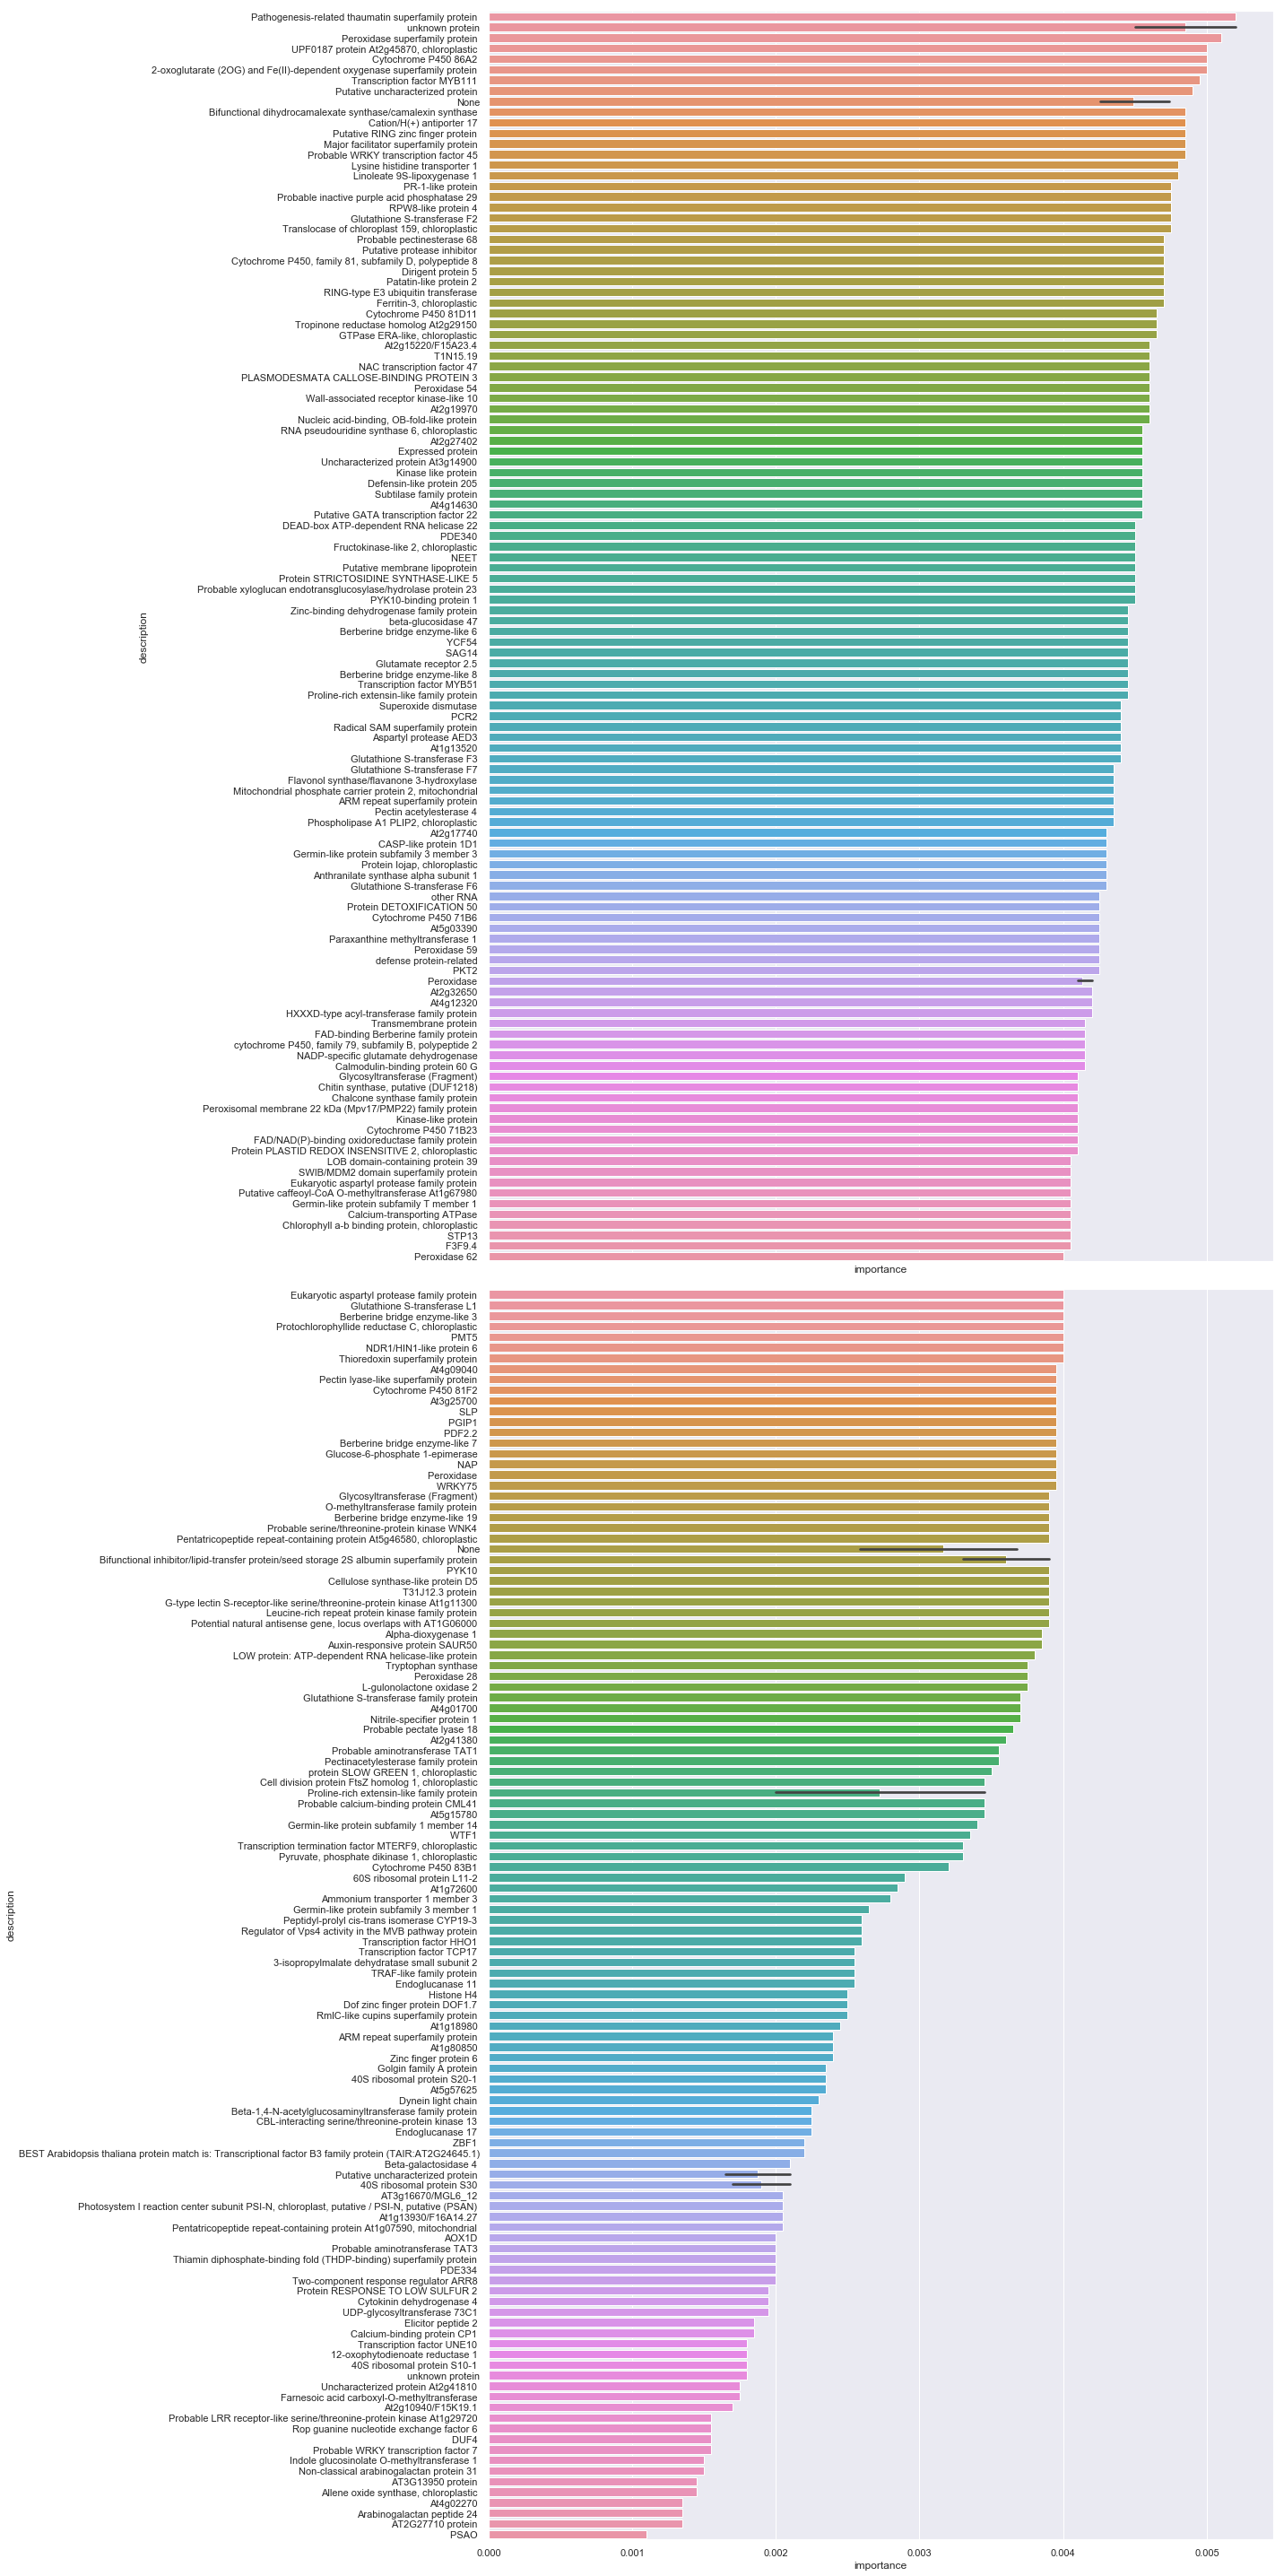
\includegraphics[width=.9\linewidth]{obipy-resources/93e2fbf76ed477962282ae99767b8408de4d3ed9/1b47b6aac6dd71371ddfe0c230d6ff5c321ce636.png}
\end{center}

\section{Selecting genes for cerk at 6hr C/W}
\label{sec:orgfeaf414}
\subsection{RFE selecting 25 genes}
\label{sec:org37ece66}
\begin{minted}[frame=lines,linenos=true,fontfamily=Monaco]{ipython}

from sklearn.feature_selection import RFE, RFECV
from sklearn.linear_model import LogisticRegression

# load data
DE_pairings_6hr = read_xl('/Users/hughesn/PHD/Transcripts/Data/pairings_6hr.xlsx')
sig = DE_pairings_05hr[DE_pairings_05hr['padj'] < 0.05]
sig = sig['log2FoldChange'].sort_values()
locs = sig.index
df = counts.loc[locs][[c for c in counts.columns if ('6h' in c and 'cer' in c)]].T
df = df.loc[:,~df.columns.duplicated()]
df = df[[c for c in set(df.columns.values)]]
\end{minted}

\begin{minted}[frame=lines,linenos=true,fontfamily=Monaco]{ipython}
# Feature Extraction with RFE
X = df.values
y = [y.rsplit('_',1)[0] for y in df.reset_index()['index']]
# feature extraction
model = LogisticRegression()
rfe = RFE(model, n_features_to_select=25)
fit = rfe.fit(X, y)
print("Num Features: {0}".format(fit.n_features_))
print("Selected Features: {0}".format(fit.support_))
print("Feature Ranking: {0}".format(fit.ranking_))
\end{minted}

Num Features: 25\\
Selected Features: [False False False \ldots{} False False False]\\
Feature Ranking: [1495 3444 1024 \ldots{} 3880 3146  939]\\


\begin{minted}[frame=lines,linenos=true,fontfamily=Monaco]{ipython}
genes = []
for r,f in zip(fit.ranking_, df.columns.values):
      if r ==1:
            genes.append(f)
get_gene_names(genes)
\end{minted}

\begin{center}
\begin{tabular}{rlll}
 & incoming & name & description\\
\hline
0 & AT5G57540 & XTH13 & Putative xyloglucan endotransglucosylase/hydrolase protein 13\\
1 & AT4G22475 & AT4G22475 & Transmembrane protein\\
2 & AT3G53150 & UGT73D1 & UDP-glucosyl transferase 73D1\\
3 & AT5G42800 & DFRA & Dihydroflavonol reductase\\
4 & AT3G01840 & LYK2 & Protein LYK2\\
5 & AT1G71030 & ATMYBL2 & At1g71030/F23N20\_2\\
6 & AT5G38930 & AT5G38930 & Germin-like protein subfamily 1 member 10\\
7 & AT4G23680 & AT4G23680 & AT4g23680/F9D16\_150\\
8 & AT4G23030 & DTX49 & Protein DETOXIFICATION 49\\
9 & AT5G45240 & AT5G45240 & Disease resistance protein (TIR-NBS-LRR class)\\
10 & AT5G49360 & BXL1 & Beta-D-xylosidase 1\\
11 & AT2G19190 & SIRK & Senescence-induced receptor-like serine/threonine-protein kinase\\
12 & AT2G28630 & KCS12 & 3-ketoacyl-CoA synthase 12\\
13 & AT1G62500 & AT1G62500 & Bifunctional inhibitor/lipid-transfer protein/seed storage 2S albumin superfamily protein\\
14 & AT5G40400 & AT5G40400 & Pentatricopeptide repeat (PPR) superfamily protein\\
15 & AT4G22485 & AT4G22485 & Bifunctional inhibitor/lipid-transfer protein/seed storage 2S albumin superfamily protein\\
16 & AT4G22495 & AT4G22495 & None\\
17 & AT3G60415 & AT3G60415 & At3g60420\\
18 & AT2G35980 & NHL10 & NDR1/HIN1-like protein 10\\
19 & AT2G38530 & LTP2 & Non-specific lipid-transfer protein\\
20 & AT4G04700 & CPK27 & Calcium-dependent protein kinase 27\\
21 & AT2G38210 & PDX1L4 & Pyridoxal 5'-phosphate synthase PDX1-like 4\\
22 & AT5G50790 & SWEET10 & Bidirectional sugar transporter SWEET10\\
23 & AT4G04540 & CRK39 & Putative cysteine-rich receptor-like protein kinase 39\\
24 & AT1G70175 & AT1G70175 & None\\
\end{tabular}
\end{center}


\subsubsection{Forest on this RFE set}
\label{sec:org28064f8}

\begin{minted}[frame=lines,linenos=true,fontfamily=Monaco]{ipython}
rfe_forest = counts.loc[genes][[c for c in counts.columns if ('6h' in c and 'cer' in c)]].T
rfe_forest = rfe_forest.loc[:,~rfe_forest.columns.duplicated()]
rfe_forest = rfe_forest[[c for c in set(rfe_forest.columns.values)]]

feat_labels = rfe_forest.columns.values
y = [d.rsplit('_', 1)[0] for d in rfe_forest.index.values]

X_train, X_test, y_train, y_test = train_test_split(rfe_forest.values, y, test_size=1, random_state=42)
forest = RandomForestClassifier(n_estimators=20000, random_state=1, n_jobs=-1)
forest.fit(X_train, y_train)
res = {k: v for k, v in sorted(
    zip(feat_labels, forest.feature_importances_), key=lambda x: x[1], reverse=True)}
res_df = pd.DataFrame(list(res.items()), columns=[
                      'gene', 'importance']).set_index('gene')
names = get_gene_names(list(res_df.index))
res_df = pd.merge(res_df, names, left_index=True, right_on='incoming').rename(
    columns={'incoming': 'gene'}).set_index('gene').sort_values('importance', ascending=False)
res_df
\end{minted}

\begin{center}
\begin{tabular}{lrll}
gene & importance & name & description\\
\hline
AT5G38930 & 0.04515 & AT5G38930 & Germin-like protein subfamily 1 member 10\\
AT4G04540 & 0.04435 & CRK39 & Putative cysteine-rich receptor-like protein kinase 39\\
AT5G40400 & 0.04295 & AT5G40400 & Pentatricopeptide repeat (PPR) superfamily protein\\
AT3G60415 & 0.0426 & AT3G60415 & At3g60420\\
AT1G70175 & 0.04245 & AT1G70175 & None\\
AT4G23030 & 0.04215 & DTX49 & Protein DETOXIFICATION 49\\
AT5G50790 & 0.04195 & SWEET10 & Bidirectional sugar transporter SWEET10\\
AT4G22485 & 0.0419 & AT4G22485 & Bifunctional inhibitor/lipid-transfer protein/seed storage 2S albumin superfamily protein\\
AT5G45240 & 0.0418 & AT5G45240 & Disease resistance protein (TIR-NBS-LRR class)\\
AT2G28630 & 0.04175 & KCS12 & 3-ketoacyl-CoA synthase 12\\
AT2G38530 & 0.04165 & LTP2 & Non-specific lipid-transfer protein\\
AT2G19190 & 0.04165 & SIRK & Senescence-induced receptor-like serine/threonine-protein kinase\\
AT1G62500 & 0.0416 & AT1G62500 & Bifunctional inhibitor/lipid-transfer protein/seed storage 2S albumin superfamily protein\\
AT5G57540 & 0.04145 & XTH13 & Putative xyloglucan endotransglucosylase/hydrolase protein 13\\
AT4G04700 & 0.04115 & CPK27 & Calcium-dependent protein kinase 27\\
AT2G38210 & 0.04025 & PDX1L4 & Pyridoxal 5'-phosphate synthase PDX1-like 4\\
AT2G35980 & 0.04 & NHL10 & NDR1/HIN1-like protein 10\\
AT3G01840 & 0.0397 & LYK2 & Protein LYK2\\
AT3G53150 & 0.0392 & UGT73D1 & UDP-glucosyl transferase 73D1\\
AT5G42800 & 0.0222 & DFRA & Dihydroflavonol reductase\\
AT4G22475 & 0.0217 & AT4G22475 & Transmembrane protein\\
AT4G22495 & 0.021 & AT4G22495 & None\\
AT1G71030 & 0.02055 & ATMYBL2 & At1g71030/F23N20\_2\\
AT5G49360 & 0.01745 & BXL1 & Beta-D-xylosidase 1\\
AT4G23680 & 0.01635 & AT4G23680 & AT4g23680/F9D16\_150\\
\end{tabular}
\end{center}

\begin{minted}[frame=lines,linenos=true,fontfamily=Monaco]{ipython}
fig, ax = plt.subplots(1, figsize=(20,20))
sns.barplot(data=res_df.reset_index(), y='description', x='importance', ax=ax)
plt.tight_layout()
\end{minted}

\begin{verbatim}
<Figure size 1440x1440 with 1 Axes>
\end{verbatim}


\begin{center}
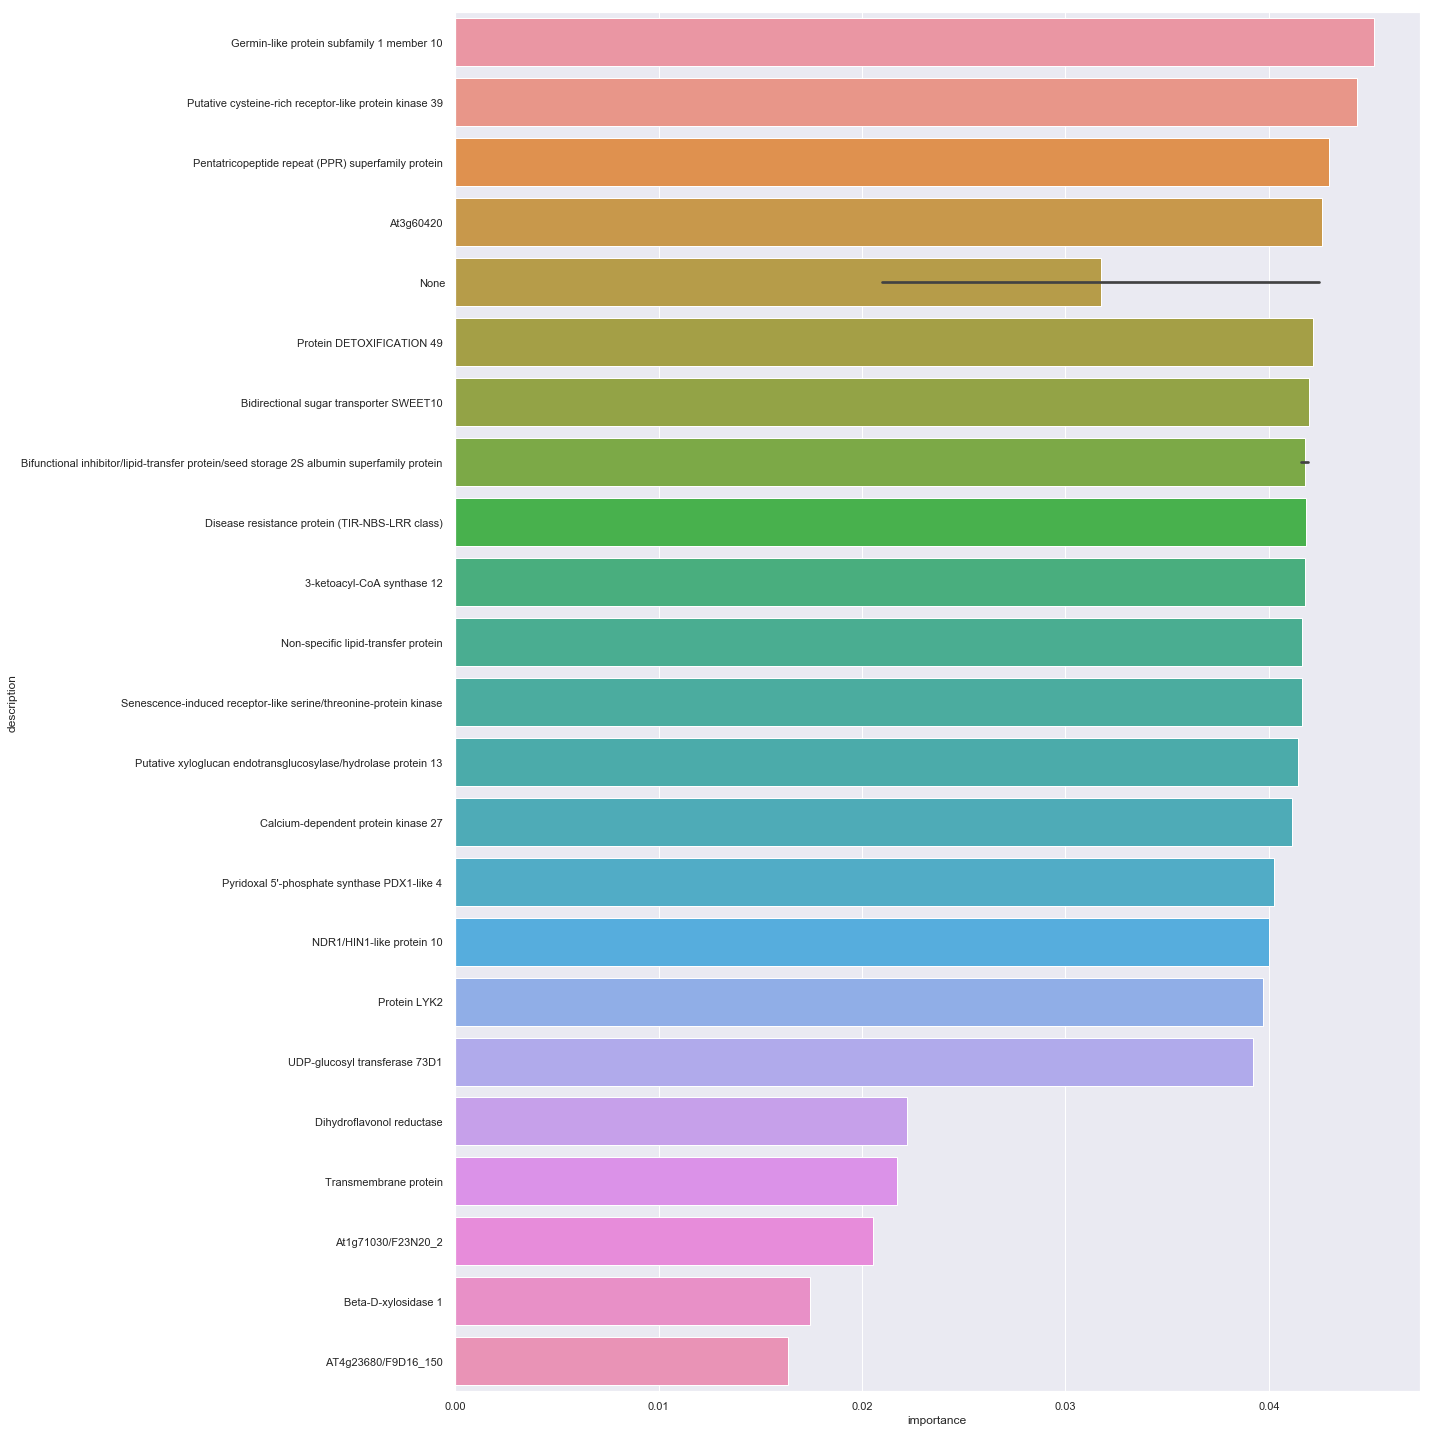
\includegraphics[width=.9\linewidth]{obipy-resources/93e2fbf76ed477962282ae99767b8408de4d3ed9/823bb9a59b4378bbd61f075dc9aba91fb69f829f.png}
\end{center}


\subsection{RFE selecting 250 genes}
\label{sec:org7a27be5}
\begin{minted}[frame=lines,linenos=true,fontfamily=Monaco]{ipython}
from sklearn.feature_selection import RFE, RFECV
from sklearn.linear_model import LogisticRegression

# load data
DE_pairings_6hr = read_xl('/Users/hughesn/PHD/Transcripts/Data/pairings_6hr.xlsx')
sig = DE_pairings_05hr[DE_pairings_05hr['padj'] < 0.05]
sig = sig['log2FoldChange'].sort_values()
locs = sig.index
df = counts.loc[locs][[c for c in counts.columns if ('6h' in c and 'cer' in c)]].T
df = df.loc[:,~df.columns.duplicated()]
df = df[[c for c in set(df.columns.values)]]
\end{minted}

\begin{minted}[frame=lines,linenos=true,fontfamily=Monaco]{ipython}
# Feature Extraction with RFE
X = df.values
y = [y.rsplit('_',1)[0] for y in df.reset_index()['index']]
# feature extraction
model = LogisticRegression()
rfe = RFE(model, n_features_to_select=250)
fit = rfe.fit(X, y)
print("Num Features: {0}".format(fit.n_features_))
print("Selected Features: {0}".format(fit.support_))
print("Feature Ranking: {0}".format(fit.ranking_))
\end{minted}

Num Features: 250\\
Selected Features: [False False False \ldots{} False False False]\\
Feature Ranking: [1270 3219  799 \ldots{} 3655 2921  714]\\


\begin{minted}[frame=lines,linenos=true,fontfamily=Monaco]{ipython}
genes = []
for r,f in zip(fit.ranking_, df.columns.values):
      if r ==1:
            genes.append(f)
get_gene_names(genes)
\end{minted}



\begin{center}
\begin{tabular}{rlll}
 & incoming & name & description\\
\hline
0 & AT4G26560 & CBL7 & Calcineurin B-like protein 7\\
1 & AT1G73805 & SARD1 & Protein SAR DEFICIENT 1\\
2 & AT1G08630 & THA1 & Probable low-specificity L-threonine aldolase 1\\
3 & AT1G19330 & AT1G19330 & unknown protein\\
4 & AT5G58620 & AT5G58620 & Zinc finger CCCH domain-containing protein 66\\
5 & AT3G22600 & AT3G22600 & AT3g22600/F16J14\_17\\
6 & AT4G23670 & AT4G23670 & AT4G23670 protein\\
7 & AT1G13530 & AT1G13530 & Protein of unknown function (DUF1262)\\
8 & AT5G40170 & AtRLP54 & Receptor-like protein 54\\
9 & AT3G22886 & MIR167A & MIR167A\\
10 & AT5G45340 & CYP707A3 & Abscisic acid 8'-hydroxylase 3\\
11 & AT5G57540 & XTH13 & Putative xyloglucan endotransglucosylase/hydrolase protein 13\\
12 & AT5G52670 & AT5G52670 & Copper transport protein family\\
13 & AT4G03600 & AT4G03600 & Pyrroline-5-carboxylate reductase\\
14 & AT1G29460 & AT1G29460 & SAUR-like auxin-responsive protein family\\
15 & AT1G72240 & AT1G72240 & Uncharacterized protein T9N14.5\\
16 & AT1G67856 & AT1G67856 & RING/U-box superfamily protein\\
17 & AT1G23550 & SRO2 & Probable inactive poly\\
18 & AT2G47800 & ABCC4 & ABC transporter C family member 4\\
19 & AT4G13820 & AT4G13820 & Disease resistance like protein\\
20 & AT4G22475 & AT4G22475 & Transmembrane protein\\
21 & AT4G14860 & OFP11 & Transcription repressor OFP11\\
22 & AT5G19890 & PER59 & Peroxidase 59\\
23 & AT5G44578 & AT5G44578 & unknown protein\\
24 & AT3G53150 & UGT73D1 & UDP-glucosyl transferase 73D1\\
25 & AT4G22490 & AT4G22490 & Bifunctional inhibitor/lipid-transfer protein/seed storage 2S albumin superfamily protein\\
26 & AT2G02880 & AT2G02880 & Mucin-like protein\\
27 & AT5G25250 & FLOT1 & Flotillin-like protein 1\\
28 & AT3G52060 & AT3G52060 & GnTL\\
29 & AT5G57345 & AT5G57345 & At5g57345\\
30 & AT1G77640 & ERF013 & Ethylene-responsive transcription factor ERF013\\
31 & AT4G14450 & AT4G14450 & Uncharacterized protein At4g14450, chloroplastic\\
32 & AT1G76680 & OPR1 & 12-oxophytodienoate reductase 1\\
33 & AT5G61570 & AT5G61570 & Protein kinase superfamily protein\\
34 & AT5G42800 & DFRA & Dihydroflavonol reductase\\
35 & AT2G02990 & RNS1 & Ribonuclease 1\\
36 & AT5G43160 & QWRF9 & Family of unknown function (DUF566)\\
37 & AT1G55420 & EDA11 & Cysteine/Histidine-rich C1 domain family protein\\
38 & AT4G23700 & CHX17 & Cation/H(+) antiporter 17\\
39 & AT3G29170 & AT3G29170 & At3g29170\\
40 & AT1G72910 & AT1G72910 & Similar to part of disease resistance protein\\
41 & AT4G11660 & HSFB2B & Heat stress transcription factor B-2b\\
42 & AT1G14170 & AT1G14170 & F7A19.25 protein\\
43 & AT3G28740 & CYP81D11 & Cytochrome P450 81D11\\
44 & AT5G60800 & AT5G60800 & Heavy metal transport/detoxification superfamily protein\\
45 & AT2G15220 & AT2G15220 & At2g15220/F15A23.4\\
46 & AT3G28580 & AT3G28580 & AAA-ATPase At3g28580\\
47 & AT1G29500 & SAUR66 & Auxin-responsive protein SAUR66\\
48 & AT1G61610 & AT1G61610 & Serine/threonine-protein kinase\\
49 & AT1G22500 & ATL15 & E3 ubiquitin-protein ligase ATL15\\
50 & AT3G08870 & AT3G08870 & Concanavalin A-like lectin protein kinase family protein\\
51 & AT2G36790 & UGT73C6 & Glycosyltransferase (Fragment)\\
52 & AT1G15100 & RHA2A & E3 ubiquitin-protein ligase RHA2A\\
53 & AT5G10520 & RBK1 & RBK1\\
54 & AT3G46930 & AT3G46930 & Protein kinase superfamily protein\\
55 & AT1G15010 & AT1G15010 & Mediator of RNA polymerase II transcription subunit\\
56 & AT1G78460 & AT1G78460 & AT1G78460 protein\\
57 & AT1G61860 & AT1G61860 & Protein kinase superfamily protein\\
58 & AT4G35070 & AT4G35070 & At4g35070\\
59 & AT5G11680 & AT5G11680 & Classical AGP protein\\
60 & AT5G43790 & PCMP-E30 & Pentatricopeptide repeat-containing protein At5g43790\\
61 & AT1G54970 & PRP1 & Proline-rich protein 1\\
62 & AT5G43180 & AT5G43180 & At5g43180\\
63 & AT4G17500 & ERF1A & Ethylene-responsive transcription factor 1A\\
64 & AT4G01390 & AT4G01390 & TRAF-like family protein\\
65 & AT2G45480 & GRF9 & Growth-regulating factor 9\\
66 & AT1G51850 & AT1G51850 & Leucine-rich repeat protein kinase family protein\\
67 & AT1G07135 & AT1G07135 & At1g07135\\
68 & AT1G51270 & AT1G51270 & Vesicle-associated protein 1-4\\
69 & AT3G47090 & AT3G47090 & Leucine-rich repeat protein kinase family protein\\
70 & AT2G37100 & AT2G37100 & Protamine P1 family protein\\
71 & AT1G36640 & AT1G36640 & Transmembrane protein\\
72 & AT1G07530 & SCL14 & AT1G07530 protein\\
73 & AT1G05675 & UGT74E1 & Glycosyltransferase (Fragment)\\
74 & AT1G21100 & IGMT1 & Indole glucosinolate O-methyltransferase 1\\
75 & AT1G35710 & AT1G35710 & Probable leucine-rich repeat receptor-like protein kinase At1g35710\\
76 & AT3G02130 & RPK2 & LRR receptor-like serine/threonine-protein kinase RPK2\\
77 & AT3G01840 & LYK2 & Protein LYK2\\
78 & AT5G48880 & KAT5 & PKT2\\
79 & AT1G71030 & ATMYBL2 & At1g71030/F23N20\_2\\
80 & AT1G62610 & AT1G62610 & NAD(P)-binding Rossmann-fold superfamily protein\\
81 & AT1G51860 & AT1G51860 & Probable LRR receptor-like serine/threonine-protein kinase At1g51860\\
82 & AT2G22980 & SCPL13 & Serine carboxypeptidase-like 13\\
83 & AT1G24147 & AT1G24147 & Transmembrane protein\\
84 & AT4G22080 & RHS14 & Probable pectate lyase 16\\
85 & AT5G38930 & AT5G38930 & Germin-like protein subfamily 1 member 10\\
86 & AT5G26340 & STP13 & STP13\\
87 & AT2G25460 & AT2G25460 & CONTAINS InterPro DOMAIN/s: C2 calcium-dependent membrane targeting (InterPro:IPR000008)\\
88 & AT2G20142 & AT2G20142 & Toll-Interleukin-Resistance (TIR) domain family protein\\
89 & AT5G59070 & AT5G59070 & UDP-Glycosyltransferase superfamily protein\\
90 & AT4G39830 & AT4G39830 & At4g39830\\
91 & AT2G39980 & AT2G39980 & At2g39980/T28M21.14\\
92 & AT4G13180 & AT4G13180 & AT4g13180/F17N18\_70\\
93 & AT4G28490 & RLK5 & Receptor-like protein kinase 5\\
94 & AT1G66090 & AT1G66090 & Disease resistance protein (TIR-NBS class)\\
95 & AT4G08950 & EXO & Protein EXORDIUM\\
96 & AT2G25125 & AT2G25125 & None\\
97 & AT2G26560 & PLP2 & Patatin-like protein 2\\
98 & AT4G23680 & AT4G23680 & AT4g23680/F9D16\_150\\
99 & AT4G23030 & DTX49 & Protein DETOXIFICATION 49\\
100 & AT5G45240 & AT5G45240 & Disease resistance protein (TIR-NBS-LRR class)\\
101 & AT2G32660 & AtRLP22 & Receptor like protein 22\\
102 & AT3G13650 & DIR7 & Dirigent protein 7\\
103 & AT5G10650 & AT5G10650 & At5g10650\\
104 & AT5G20670 & AT5G20670 & At5g20670\\
105 & AT5G65500 & AT5G65500 & U-box domain-containing protein kinase family protein\\
106 & AT4G21380 & SD18 & Receptor-like serine/threonine-protein kinase SD1-8\\
107 & AT4G11890 & AT4G11890 & Protein kinase superfamily protein\\
108 & AT5G03830 & AT5G03830 & CDK inhibitor P21 binding protein\\
109 & AT4G33720 & AT4G33720 & AT4g33720/T16L1\_210\\
110 & AT5G49360 & BXL1 & Beta-D-xylosidase 1\\
111 & AT4G27980 & AT4G27980 & Domain of unknown function (DUF3444)\\
112 & AT2G19190 & SIRK & Senescence-induced receptor-like serine/threonine-protein kinase\\
113 & AT4G24810 & AT4G24810 & Protein kinase superfamily protein\\
114 & AT3G19850 & AT3G19850 & BTB/POZ domain-containing protein At3g19850\\
115 & AT5G05300 & AT5G05300 & Gb\\
116 & AT1G20870 & IDM3 & Increased DNA methylation 3\\
117 & AT2G42840 & PDF1 & Protodermal factor 1\\
118 & AT2G24850 & TAT3 & Probable aminotransferase TAT3\\
119 & AT1G33760 & ERF022 & Ethylene-responsive transcription factor ERF022\\
120 & AT3G48450 & AT3G48450 & At3g48450\\
121 & AT5G57560 & XTH22 & Xyloglucan endotransglucosylase/hydrolase\\
122 & AT2G28630 & KCS12 & 3-ketoacyl-CoA synthase 12\\
123 & AT4G05910 & AT4G05910 & None\\
124 & AT2G21050 & LAX2 & Auxin transporter-like protein 2\\
125 & AT1G62500 & AT1G62500 & Bifunctional inhibitor/lipid-transfer protein/seed storage 2S albumin superfamily protein\\
126 & AT1G72900 & AT1G72900 & Similar to part of disease resistance protein\\
127 & AT1G70190 & AT1G70190 & F20P5.9 protein\\
128 & AT2G22790 & AT2G22790 & Uncharacterized protein At2g22790\\
129 & AT1G67855 & AT1G67855 & unknown protein\\
130 & AT1G69790 & PBL18 & Probable serine/threonine-protein kinase PBL18\\
131 & AT3G25790 & HHO1 & Transcription factor HHO1\\
132 & AT5G65410 & ZHD1 & Zinc-finger homeodomain protein 1\\
133 & AT3G29400 & ATEXO70E1 & Exocyst subunit Exo70 family protein\\
134 & AT1G31050 & AT1G31050 & basic helix-loop-helix (bHLH) DNA-binding superfamily protein\\
135 & AT1G50750 & AT1G50750 & Plant mobile domain protein family\\
136 & AT4G11000 & AT4G11000 & Ankyrin repeat family protein\\
137 & AT5G40400 & AT5G40400 & Pentatricopeptide repeat (PPR) superfamily protein\\
138 & AT4G21903 & AT4G21903 & Protein DETOXIFICATION\\
139 & AT2G35640 & AT2G35640 & Homeodomain-like superfamily protein\\
140 & AT5G46570 & BSK2 & Serine/threonine-protein kinase BSK2\\
141 & AT1G12780 & UGE1 & Bifunctional UDP-glucose 4-epimerase and UDP-xylose 4-epimerase 1\\
142 & AT3G11080 & AtRLP35 & Receptor-like protein 35\\
143 & AT2G46600 & KIC & Calcium-binding protein KIC\\
144 & AT4G22485 & AT4G22485 & Bifunctional inhibitor/lipid-transfer protein/seed storage 2S albumin superfamily protein\\
145 & AT4G23210 & CRK13 & Cysteine-rich receptor-like protein kinase 13\\
146 & AT5G41740 & AT5G41740 & Disease resistance protein (TIR-NBS-LRR class) family\\
147 & AT1G66500 & PCFS1 & Polyadenylation and cleavage factor homolog 1\\
148 & AT3G16400 & NSP1 & Nitrile-specifier protein 1\\
149 & AT3G51570 & AT3G51570 & Disease resistance protein (TIR-NBS-LRR class) family\\
150 & AT3G43580 & AT3G43580 & At3g43580\\
151 & AT1G02310 & MAN1 & MAN1\\
152 & AT2G41231 & AT2G41231 & unknown protein.\\
153 & AT4G33220 & PME44 & Probable pectinesterase/pectinesterase inhibitor 44\\
154 & AT4G22495 & AT4G22495 & None\\
155 & AT3G49620 & DIN11 & Probable 2-oxoglutarate-dependent dioxygenase DIN11\\
156 & AT3G46090 & ZAT7 & ZAT7\\
157 & AT3G55090 & ABCG16 & ABC transporter G family member 16\\
158 & AT3G60415 & AT3G60415 & At3g60420\\
159 & AT1G55020 & LOX1 & Linoleate 9S-lipoxygenase 1\\
160 & AT1G59860 & HSP17.6A & 17.6 kDa class I heat shock protein 1\\
161 & AT3G18950 & AT3G18950 & En/Spm-like transposon protein-like\\
162 & AT5G21900 & AT5G21900 & At5g21900\\
163 & AT2G35980 & NHL10 & NDR1/HIN1-like protein 10\\
164 & AT1G75240 & ZHD5 & ZHD5\\
165 & AT5G51670 & AT5G51670 & Similarity to unknown protein\\
166 & AT3G01175 & AT3G01175 & Transmembrane protein\\
167 & AT1G27370 & SPL10 & Squamosa promoter-binding-like protein 10\\
168 & AT2G38530 & LTP2 & Non-specific lipid-transfer protein\\
169 & AT4G31875 & AT4G31875 & At4g31872/At4g31872\\
170 & AT3G50800 & AT3G50800 & Uncharacterized protein At3g50800\\
171 & AT5G16170 & AT5G16170 & At5g16170\\
172 & AT5G27830 & AT5G27830 & FUNCTIONS IN: molecular\_function unknown\\
173 & AT3G44860 & FAMT & Farnesoic acid carboxyl-O-methyltransferase\\
174 & AT1G13520 & AT1G13520 & At1g13520\\
175 & AT2G21210 & AT2G21210 & SAUR-like auxin-responsive protein family\\
176 & AT1G22890 & AT1G22890 & AT1G22890 protein\\
177 & AT3G23120 & AtRLP38 & Receptor-like protein 38\\
178 & AT5G51465 & AT5G51465 & None\\
179 & AT3G10710 & PME24 & Putative pectinesterase/pectinesterase inhibitor 24\\
180 & AT4G04700 & CPK27 & Calcium-dependent protein kinase 27\\
181 & AT1G44446 & CAO & CH1\\
182 & AT4G01870 & AT4G01870 & tolB protein-related\\
183 & AT2G29720 & CTF2B & FAD/NAD(P)-binding oxidoreductase family protein\\
184 & AT2G38210 & PDX1L4 & Pyridoxal 5'-phosphate synthase PDX1-like 4\\
185 & AT3G46280 & AT3G46280 & Kinase-like protein\\
186 & AT2G07698 & AT2G07698 & ATPase, F1 complex, alpha subunit protein\\
187 & AT1G14480 & AT1G14480 & Ankyrin repeat family protein\\
188 & AT4G22510 & AT4G22510 & unknown protein\\
189 & AT3G54890 & LHCA1 & Chlorophyll a-b binding protein, chloroplastic\\
190 & AT4G26800 & AT4G26800 & Pentatricopeptide repeat-containing protein At4g26800\\
191 & AT4G19520 & AT4G19520 & Probable disease resistance protein At4g19520\\
192 & AT5G27490 & AT5G27490 & Protein YIPF\\
193 & AT5G66000 & AT5G66000 & Uncharacterized protein At5g66000\\
194 & AT2G38580 & AT2G38580 & Mitochondrial ATP synthase D chain-related protein\\
195 & AT5G50790 & SWEET10 & Bidirectional sugar transporter SWEET10\\
196 & AT3G54200 & AT3G54200 & Late embryogenesis abundant (LEA) hydroxyproline-rich glycoprotein family\\
197 & AT2G46440 & CNGC11 & Cyclic nucleotide-gated ion channel 11\\
198 & ATCG00760 & RPL36 & 50S ribosomal protein L36, chloroplastic\\
199 & AT5G16800 & AT5G16800 & Acyl-CoA N-acyltransferases (NAT) superfamily protein\\
200 & AT3G63255 & AT3G63255 & None\\
201 & AT2G22860 & PSK2 & Phytosulfokines 2\\
202 & AT3G05200 & ATL6 & E3 ubiquitin-protein ligase ATL6\\
203 & AT5G56870 & BGAL4 & Beta-galactosidase 4\\
204 & AT4G30570 & AT4G30570 & Probable mannose-1-phosphate guanylyltransferase 3\\
205 & AT2G46750 & GULLO2 & L-gulonolactone oxidase 2\\
206 & AT4G33050 & EDA39 & calmodulin-binding family protein\\
207 & AT1G72280 & AERO1 & Like disulfide bond formation protein\\
208 & AT1G63350 & AT1G63350 & Disease resistance protein (CC-NBS-LRR class) family\\
209 & AT4G17490 & ERF6 & Ethylene-responsive transcription factor 6\\
210 & AT5G65207 & AT5G65207 & Uncharacterized protein At5g65207\\
211 & AT5G06730 & PER54 & Peroxidase 54\\
212 & AT5G48657 & AT5G48657 & defense protein-related\\
213 & AT3G21780 & UGT71B6 & UDP-glycosyltransferase 71B6\\
214 & AT5G46500 & AT5G46500 & Protein VARIATION IN COMPOUND TRIGGERED ROOT growth protein\\
215 & AT4G38840 & AT4G38840 & At4g38840\\
216 & AT4G35180 & LHT7 & Lysine histidine transporter-like 7\\
217 & AT1G17345 & SAUR77 & Auxin-responsive protein SAUR77\\
218 & AT1G56430 & NAS4 & Probable nicotianamine synthase 4\\
219 & AT4G35110 & AT4G35110 & Phospholipase-like protein (PEARLI 4) family protein\\
220 & AT5G28630 & AT5G28630 & Glycine-rich protein\\
221 & AT4G35770 & STR15 & SEN1\\
222 & AT3G21230 & 4CL4 & 4-coumarate--CoA ligase 4\\
223 & AT1G26761 & AT1G26761 & Arabinanase/levansucrase/invertase\\
224 & AT2G19210 & AT2G19210 & Putative leucine-rich repeat receptor-like protein kinase At2g19210\\
225 & AT3G55980 & SZF1 & Salt-inducible zinc finger 1\\
226 & AT3G61280 & AT3G61280 & Glycosyltransferase\\
227 & AT3G56260 & AT3G56260 & At3g56260\\
228 & AT4G01970 & AtSTS & stachyose synthase\\
229 & AT1G51890 & AT1G51890 & Leucine-rich repeat protein kinase family protein\\
230 & AT5G42380 & CML37 & Calcium-binding protein CML37\\
231 & AT2G23210 & AT2G23210 & UDP-Glycosyltransferase superfamily protein\\
232 & AT3G04210 & AT3G04210 & At3g04210/T6K12\_17\\
233 & AT5G65860 & AT5G65860 & Ankyrin repeat family protein\\
234 & AT4G19230 & CYP707A1 & Cytochrome P450, family 707, subfamily A, polypeptide 1\\
235 & AT1G74930 & ERF018 & Ethylene-responsive transcription factor ERF018\\
236 & AT4G04540 & CRK39 & Putative cysteine-rich receptor-like protein kinase 39\\
237 & AT5G40000 & AT5G40000 & AAA-ATPase At5g40000\\
238 & AT1G17610 & CHS1 & Disease resistance protein CHS1\\
239 & AT4G24110 & AT4G24110 & NADP-specific glutamate dehydrogenase\\
240 & AT1G25560 & TEM1 & AP2/ERF and B3 domain-containing transcription repressor TEM1\\
241 & AT1G70175 & AT1G70175 & None\\
242 & AT1G68570 & NPF3.1 & Protein NRT1/ PTR FAMILY 3.1\\
243 & AT2G23120 & AT2G23120 & Expressed protein\\
244 & AT5G54569 & AT5G54569 & other RNA\\
245 & AT3G15740 & AT3G15740 & RING/U-box superfamily protein\\
246 & AT1G72645 & AT1G72645 & At1g72645\\
247 & AT1G51660 & MKK4 & MKK4\\
248 & AT3G62680 & PRP3 & Proline-rich protein 3\\
249 & AT1G14870 & PCR2 & PCR2\\
\end{tabular}
\end{center}


\paragraph{Forest on this RFE set}
\label{sec:org357075a}

\begin{minted}[frame=lines,linenos=true,fontfamily=Monaco]{ipython}
rfe_forest = counts.loc[genes][[c for c in counts.columns if ('6h' in c and 'cer' in c)]].T
rfe_forest = rfe_forest.loc[:,~rfe_forest.columns.duplicated()]
rfe_forest = rfe_forest[[c for c in set(rfe_forest.columns.values)]]

feat_labels = rfe_forest.columns.values
y = [d.rsplit('_', 1)[0] for d in rfe_forest.index.values]

X_train, X_test, y_train, y_test = train_test_split(rfe_forest.values, y, test_size=1, random_state=42)
forest = RandomForestClassifier(n_estimators=20000, random_state=1, n_jobs=-1)
forest.fit(X_train, y_train)
res = {k: v for k, v in sorted(
    zip(feat_labels, forest.feature_importances_), key=lambda x: x[1], reverse=True)}
res_df = pd.DataFrame(list(res.items()), columns=[
                      'gene', 'importance']).set_index('gene')
names = get_gene_names(list(res_df.index))
res_df = pd.merge(res_df, names, left_index=True, right_on='incoming').rename(
    columns={'incoming': 'gene'}).set_index('gene').sort_values('importance', ascending=False)
res_df
\end{minted}

\begin{center}
\begin{tabular}{lrll}
gene & importance & name & description\\
\hline
AT1G61610 & 0.00575 & AT1G61610 & Serine/threonine-protein kinase\\
AT3G54200 & 0.0056 & AT3G54200 & Late embryogenesis abundant (LEA) hydroxyproline-rich glycoprotein family\\
AT1G66500 & 0.0054 & PCFS1 & Polyadenylation and cleavage factor homolog 1\\
AT1G73805 & 0.00535 & SARD1 & Protein SAR DEFICIENT 1\\
AT1G70190 & 0.00525 & AT1G70190 & F20P5.9 protein\\
AT5G66000 & 0.00515 & AT5G66000 & Uncharacterized protein At5g66000\\
AT3G02130 & 0.0051 & RPK2 & LRR receptor-like serine/threonine-protein kinase RPK2\\
AT4G01870 & 0.0051 & AT4G01870 & tolB protein-related\\
AT1G36640 & 0.0051 & AT1G36640 & Transmembrane protein\\
AT3G08870 & 0.005 & AT3G08870 & Concanavalin A-like lectin protein kinase family protein\\
AT4G24110 & 0.005 & AT4G24110 & NADP-specific glutamate dehydrogenase\\
AT5G46500 & 0.00495 & AT5G46500 & Protein VARIATION IN COMPOUND TRIGGERED ROOT growth protein\\
AT2G37100 & 0.00495 & AT2G37100 & Protamine P1 family protein\\
AT4G22485 & 0.0049 & AT4G22485 & Bifunctional inhibitor/lipid-transfer protein/seed storage 2S albumin superfamily protein\\
AT3G25790 & 0.00485 & HHO1 & Transcription factor HHO1\\
AT4G17500 & 0.00485 & ERF1A & Ethylene-responsive transcription factor 1A\\
AT1G29460 & 0.00485 & AT1G29460 & SAUR-like auxin-responsive protein family\\
AT4G11660 & 0.00485 & HSFB2B & Heat stress transcription factor B-2b\\
AT4G23700 & 0.00485 & CHX17 & Cation/H(+) antiporter 17\\
AT1G08630 & 0.00485 & THA1 & Probable low-specificity L-threonine aldolase 1\\
AT1G33760 & 0.00485 & ERF022 & Ethylene-responsive transcription factor ERF022\\
AT3G63255 & 0.00485 & AT3G63255 & None\\
AT5G21900 & 0.00485 & AT5G21900 & At5g21900\\
AT2G20142 & 0.0048 & AT2G20142 & Toll-Interleukin-Resistance (TIR) domain family protein\\
AT4G35110 & 0.0048 & AT4G35110 & Phospholipase-like protein (PEARLI 4) family protein\\
AT4G01390 & 0.0048 & AT4G01390 & TRAF-like family protein\\
AT2G19190 & 0.0048 & SIRK & Senescence-induced receptor-like serine/threonine-protein kinase\\
ATCG00760 & 0.0048 & RPL36 & 50S ribosomal protein L36, chloroplastic\\
AT1G35710 & 0.00475 & AT1G35710 & Probable leucine-rich repeat receptor-like protein kinase At1g35710\\
AT1G62610 & 0.00475 & AT1G62610 & NAD(P)-binding Rossmann-fold superfamily protein\\
AT5G27830 & 0.00475 & AT5G27830 & FUNCTIONS IN: molecular\_function unknown\\
AT1G56430 & 0.00475 & NAS4 & Probable nicotianamine synthase 4\\
AT4G19520 & 0.00475 & AT4G19520 & Probable disease resistance protein At4g19520\\
AT5G57560 & 0.00475 & XTH22 & Xyloglucan endotransglucosylase/hydrolase\\
AT3G43580 & 0.0047 & AT3G43580 & At3g43580\\
AT2G46600 & 0.0047 & KIC & Calcium-binding protein KIC\\
AT1G70175 & 0.0047 & AT1G70175 & None\\
AT4G38840 & 0.0047 & AT4G38840 & At4g38840\\
AT3G49620 & 0.0047 & DIN11 & Probable 2-oxoglutarate-dependent dioxygenase DIN11\\
AT4G35180 & 0.00465 & LHT7 & Lysine histidine transporter-like 7\\
AT4G13820 & 0.00465 & AT4G13820 & Disease resistance like protein\\
AT4G01970 & 0.00465 & AtSTS & stachyose synthase\\
AT5G26340 & 0.00465 & STP13 & STP13\\
AT1G67856 & 0.00465 & AT1G67856 & RING/U-box superfamily protein\\
AT5G59070 & 0.00465 & AT5G59070 & UDP-Glycosyltransferase superfamily protein\\
AT5G10650 & 0.00465 & AT5G10650 & At5g10650\\
AT1G17610 & 0.00465 & CHS1 & Disease resistance protein CHS1\\
AT3G01175 & 0.0046 & AT3G01175 & Transmembrane protein\\
AT1G14480 & 0.0046 & AT1G14480 & Ankyrin repeat family protein\\
AT5G45240 & 0.0046 & AT5G45240 & Disease resistance protein (TIR-NBS-LRR class)\\
AT5G54569 & 0.0046 & AT5G54569 & other RNA\\
AT4G23670 & 0.0046 & AT4G23670 & AT4G23670 protein\\
AT2G15220 & 0.00455 & AT2G15220 & At2g15220/F15A23.4\\
AT4G14450 & 0.00455 & AT4G14450 & Uncharacterized protein At4g14450, chloroplastic\\
AT2G45480 & 0.0045 & GRF9 & Growth-regulating factor 9\\
AT2G19210 & 0.0045 & AT2G19210 & Putative leucine-rich repeat receptor-like protein kinase At2g19210\\
AT4G26800 & 0.0045 & AT4G26800 & Pentatricopeptide repeat-containing protein At4g26800\\
AT5G48657 & 0.0045 & AT5G48657 & defense protein-related\\
AT4G14860 & 0.0045 & OFP11 & Transcription repressor OFP11\\
AT4G21903 & 0.0045 & AT4G21903 & Protein DETOXIFICATION\\
AT3G50800 & 0.0045 & AT3G50800 & Uncharacterized protein At3g50800\\
AT3G11080 & 0.0045 & AtRLP35 & Receptor-like protein 35\\
AT5G57345 & 0.0045 & AT5G57345 & At5g57345\\
AT3G55980 & 0.0045 & SZF1 & Salt-inducible zinc finger 1\\
AT4G35070 & 0.0045 & AT4G35070 & At4g35070\\
AT1G26761 & 0.00445 & AT1G26761 & Arabinanase/levansucrase/invertase\\
AT5G43180 & 0.00445 & AT5G43180 & At5g43180\\
AT5G51670 & 0.00445 & AT5G51670 & Similarity to unknown protein\\
AT2G23120 & 0.00445 & AT2G23120 & Expressed protein\\
AT5G57540 & 0.00445 & XTH13 & Putative xyloglucan endotransglucosylase/hydrolase protein 13\\
AT1G78460 & 0.0044 & AT1G78460 & AT1G78460 protein\\
AT4G13180 & 0.0044 & AT4G13180 & AT4g13180/F17N18\_70\\
AT2G23210 & 0.0044 & AT2G23210 & UDP-Glycosyltransferase superfamily protein\\
AT5G46570 & 0.0044 & BSK2 & Serine/threonine-protein kinase BSK2\\
AT1G20870 & 0.00435 & IDM3 & Increased DNA methylation 3\\
AT4G33220 & 0.00435 & PME44 & Probable pectinesterase/pectinesterase inhibitor 44\\
AT3G22886 & 0.00435 & MIR167A & MIR167A\\
AT5G19890 & 0.00435 & PER59 & Peroxidase 59\\
AT1G12780 & 0.00435 & UGE1 & Bifunctional UDP-glucose 4-epimerase and UDP-xylose 4-epimerase 1\\
AT1G50750 & 0.00435 & AT1G50750 & Plant mobile domain protein family\\
AT1G07530 & 0.00435 & SCL14 & AT1G07530 protein\\
AT3G13650 & 0.00435 & DIR7 & Dirigent protein 7\\
AT5G65860 & 0.00435 & AT5G65860 & Ankyrin repeat family protein\\
AT5G03830 & 0.0043 & AT5G03830 & CDK inhibitor P21 binding protein\\
AT5G40000 & 0.0043 & AT5G40000 & AAA-ATPase At5g40000\\
AT1G62500 & 0.0043 & AT1G62500 & Bifunctional inhibitor/lipid-transfer protein/seed storage 2S albumin superfamily protein\\
AT3G05200 & 0.0043 & ATL6 & E3 ubiquitin-protein ligase ATL6\\
AT3G48450 & 0.0043 & AT3G48450 & At3g48450\\
AT1G07135 & 0.00425 & AT1G07135 & At1g07135\\
AT1G55420 & 0.00425 & EDA11 & Cysteine/Histidine-rich C1 domain family protein\\
AT1G19330 & 0.00425 & AT1G19330 & unknown protein\\
AT3G46090 & 0.00425 & ZAT7 & ZAT7\\
AT3G29170 & 0.0042 & AT3G29170 & At3g29170\\
AT1G27370 & 0.0042 & SPL10 & Squamosa promoter-binding-like protein 10\\
AT3G28740 & 0.0042 & CYP81D11 & Cytochrome P450 81D11\\
AT3G60415 & 0.0042 & AT3G60415 & At3g60420\\
AT2G29720 & 0.0042 & CTF2B & FAD/NAD(P)-binding oxidoreductase family protein\\
AT5G42380 & 0.0042 & CML37 & Calcium-binding protein CML37\\
AT3G46930 & 0.0042 & AT3G46930 & Protein kinase superfamily protein\\
AT2G38580 & 0.0042 & AT2G38580 & Mitochondrial ATP synthase D chain-related protein\\
AT5G44578 & 0.0042 & AT5G44578 & unknown protein\\
AT5G41740 & 0.00415 & AT5G41740 & Disease resistance protein (TIR-NBS-LRR class) family\\
AT5G43160 & 0.00415 & QWRF9 & Family of unknown function (DUF566)\\
AT4G28490 & 0.00415 & RLK5 & Receptor-like protein kinase 5\\
AT2G39980 & 0.00415 & AT2G39980 & At2g39980/T28M21.14\\
AT5G58620 & 0.00415 & AT5G58620 & Zinc finger CCCH domain-containing protein 66\\
AT3G55090 & 0.00415 & ABCG16 & ABC transporter G family member 16\\
AT1G22890 & 0.00415 & AT1G22890 & AT1G22890 protein\\
AT5G10520 & 0.00415 & RBK1 & RBK1\\
AT2G46440 & 0.00415 & CNGC11 & Cyclic nucleotide-gated ion channel 11\\
AT3G28580 & 0.00415 & AT3G28580 & AAA-ATPase At3g28580\\
AT1G05675 & 0.00415 & UGT74E1 & Glycosyltransferase (Fragment)\\
AT2G21210 & 0.0041 & AT2G21210 & SAUR-like auxin-responsive protein family\\
AT1G68570 & 0.0041 & NPF3.1 & Protein NRT1/ PTR FAMILY 3.1\\
AT5G43790 & 0.0041 & PCMP-E30 & Pentatricopeptide repeat-containing protein At5g43790\\
AT1G72910 & 0.0041 & AT1G72910 & Similar to part of disease resistance protein\\
AT4G21380 & 0.0041 & SD18 & Receptor-like serine/threonine-protein kinase SD1-8\\
AT3G01840 & 0.0041 & LYK2 & Protein LYK2\\
AT5G65410 & 0.0041 & ZHD1 & Zinc-finger homeodomain protein 1\\
AT2G26560 & 0.0041 & PLP2 & Patatin-like protein 2\\
AT5G11680 & 0.0041 & AT5G11680 & Classical AGP protein\\
AT1G25560 & 0.0041 & TEM1 & AP2/ERF and B3 domain-containing transcription repressor TEM1\\
AT2G28630 & 0.0041 & KCS12 & 3-ketoacyl-CoA synthase 12\\
AT4G33050 & 0.0041 & EDA39 & calmodulin-binding family protein\\
AT5G50790 & 0.0041 & SWEET10 & Bidirectional sugar transporter SWEET10\\
AT1G02310 & 0.0041 & MAN1 & MAN1\\
AT2G07698 & 0.00405 & AT2G07698 & ATPase, F1 complex, alpha subunit protein\\
AT4G04540 & 0.00405 & CRK39 & Putative cysteine-rich receptor-like protein kinase 39\\
AT5G40170 & 0.00405 & AtRLP54 & Receptor-like protein 54\\
AT2G02990 & 0.00405 & RNS1 & Ribonuclease 1\\
AT2G38530 & 0.00405 & LTP2 & Non-specific lipid-transfer protein\\
AT5G65207 & 0.00405 & AT5G65207 & Uncharacterized protein At5g65207\\
AT4G04700 & 0.00405 & CPK27 & Calcium-dependent protein kinase 27\\
AT3G18950 & 0.00405 & AT3G18950 & En/Spm-like transposon protein-like\\
AT2G41231 & 0.004 & AT2G41231 & unknown protein.\\
AT5G48880 & 0.004 & KAT5 & PKT2\\
AT2G47800 & 0.004 & ABCC4 & ABC transporter C family member 4\\
AT4G23030 & 0.004 & DTX49 & Protein DETOXIFICATION 49\\
AT1G77640 & 0.004 & ERF013 & Ethylene-responsive transcription factor ERF013\\
AT1G44446 & 0.004 & CAO & CH1\\
AT4G11890 & 0.00395 & AT4G11890 & Protein kinase superfamily protein\\
AT4G26560 & 0.00395 & CBL7 & Calcineurin B-like protein 7\\
AT2G35980 & 0.00395 & NHL10 & NDR1/HIN1-like protein 10\\
AT1G75240 & 0.00395 & ZHD5 & ZHD5\\
AT1G72280 & 0.00395 & AERO1 & Like disulfide bond formation protein\\
AT2G22980 & 0.00395 & SCPL13 & Serine carboxypeptidase-like 13\\
AT1G14170 & 0.0039 & AT1G14170 & F7A19.25 protein\\
AT1G72900 & 0.0039 & AT1G72900 & Similar to part of disease resistance protein\\
AT5G25250 & 0.0039 & FLOT1 & Flotillin-like protein 1\\
AT4G03600 & 0.00385 & AT4G03600 & Pyrroline-5-carboxylate reductase\\
AT5G28630 & 0.00385 & AT5G28630 & Glycine-rich protein\\
AT2G36790 & 0.00385 & UGT73C6 & Glycosyltransferase (Fragment)\\
AT4G24810 & 0.00385 & AT4G24810 & Protein kinase superfamily protein\\
AT5G45340 & 0.0038 & CYP707A3 & Abscisic acid 8'-hydroxylase 3\\
AT5G38930 & 0.0038 & AT5G38930 & Germin-like protein subfamily 1 member 10\\
AT2G21050 & 0.0038 & LAX2 & Auxin transporter-like protein 2\\
AT5G27490 & 0.0038 & AT5G27490 & Protein YIPF\\
AT5G16170 & 0.0038 & AT5G16170 & At5g16170\\
AT5G61570 & 0.00375 & AT5G61570 & Protein kinase superfamily protein\\
AT3G53150 & 0.00375 & UGT73D1 & UDP-glucosyl transferase 73D1\\
AT1G51850 & 0.00375 & AT1G51850 & Leucine-rich repeat protein kinase family protein\\
AT3G15740 & 0.00375 & AT3G15740 & RING/U-box superfamily protein\\
AT4G19230 & 0.00375 & CYP707A1 & Cytochrome P450, family 707, subfamily A, polypeptide 1\\
AT3G62680 & 0.0037 & PRP3 & Proline-rich protein 3\\
AT4G08950 & 0.0036 & EXO & Protein EXORDIUM\\
AT3G23120 & 0.0036 & AtRLP38 & Receptor-like protein 38\\
AT2G02880 & 0.0036 & AT2G02880 & Mucin-like protein\\
AT2G35640 & 0.00355 & AT2G35640 & Homeodomain-like superfamily protein\\
AT1G72645 & 0.00355 & AT1G72645 & At1g72645\\
AT4G22080 & 0.00355 & RHS14 & Probable pectate lyase 16\\
AT1G15010 & 0.0035 & AT1G15010 & Mediator of RNA polymerase II transcription subunit\\
AT2G38210 & 0.00345 & PDX1L4 & Pyridoxal 5'-phosphate synthase PDX1-like 4\\
AT1G15100 & 0.0034 & RHA2A & E3 ubiquitin-protein ligase RHA2A\\
AT4G11000 & 0.0033 & AT4G11000 & Ankyrin repeat family protein\\
AT5G40400 & 0.00325 & AT5G40400 & Pentatricopeptide repeat (PPR) superfamily protein\\
AT1G17345 & 0.0032 & SAUR77 & Auxin-responsive protein SAUR77\\
AT5G06730 & 0.0031 & PER54 & Peroxidase 54\\
AT4G22475 & 0.00295 & AT4G22475 & Transmembrane protein\\
AT4G22495 & 0.0029 & AT4G22495 & None\\
AT1G63350 & 0.0028 & AT1G63350 & Disease resistance protein (CC-NBS-LRR class) family\\
AT2G42840 & 0.0027 & PDF1 & Protodermal factor 1\\
AT2G24850 & 0.0027 & TAT3 & Probable aminotransferase TAT3\\
AT1G55020 & 0.0027 & LOX1 & Linoleate 9S-lipoxygenase 1\\
AT1G74930 & 0.0027 & ERF018 & Ethylene-responsive transcription factor ERF018\\
AT1G24147 & 0.00265 & AT1G24147 & Transmembrane protein\\
AT1G76680 & 0.0026 & OPR1 & 12-oxophytodienoate reductase 1\\
AT1G23550 & 0.0026 & SRO2 & Probable inactive poly\\
AT4G17490 & 0.0026 & ERF6 & Ethylene-responsive transcription factor 6\\
AT3G46280 & 0.0026 & AT3G46280 & Kinase-like protein\\
AT1G21100 & 0.00255 & IGMT1 & Indole glucosinolate O-methyltransferase 1\\
AT4G35770 & 0.00255 & STR15 & SEN1\\
AT5G42800 & 0.00255 & DFRA & Dihydroflavonol reductase\\
AT3G16400 & 0.00255 & NSP1 & Nitrile-specifier protein 1\\
AT1G13530 & 0.00245 & AT1G13530 & Protein of unknown function (DUF1262)\\
AT1G66090 & 0.00245 & AT1G66090 & Disease resistance protein (TIR-NBS class)\\
AT1G29500 & 0.0024 & SAUR66 & Auxin-responsive protein SAUR66\\
AT4G23210 & 0.0024 & CRK13 & Cysteine-rich receptor-like protein kinase 13\\
AT1G51660 & 0.00235 & MKK4 & MKK4\\
AT1G59860 & 0.00235 & HSP17.6A & 17.6 kDa class I heat shock protein 1\\
AT1G54970 & 0.00235 & PRP1 & Proline-rich protein 1\\
AT5G51465 & 0.00225 & AT5G51465 & None\\
AT1G13520 & 0.00225 & AT1G13520 & At1g13520\\
AT5G20670 & 0.00225 & AT5G20670 & At5g20670\\
AT4G31875 & 0.00225 & AT4G31875 & At4g31872/At4g31872\\
AT3G19850 & 0.0022 & AT3G19850 & BTB/POZ domain-containing protein At3g19850\\
AT3G61280 & 0.0022 & AT3G61280 & Glycosyltransferase\\
AT2G46750 & 0.0022 & GULLO2 & L-gulonolactone oxidase 2\\
AT3G51570 & 0.00215 & AT3G51570 & Disease resistance protein (TIR-NBS-LRR class) family\\
AT4G27980 & 0.00215 & AT4G27980 & Domain of unknown function (DUF3444)\\
AT3G04210 & 0.00215 & AT3G04210 & At3g04210/T6K12\_17\\
AT3G10710 & 0.00215 & PME24 & Putative pectinesterase/pectinesterase inhibitor 24\\
AT1G71030 & 0.0021 & ATMYBL2 & At1g71030/F23N20\_2\\
AT2G22790 & 0.0021 & AT2G22790 & Uncharacterized protein At2g22790\\
AT1G51270 & 0.0021 & AT1G51270 & Vesicle-associated protein 1-4\\
AT3G44860 & 0.0021 & FAMT & Farnesoic acid carboxyl-O-methyltransferase\\
AT5G65500 & 0.00205 & AT5G65500 & U-box domain-containing protein kinase family protein\\
AT3G22600 & 0.00205 & AT3G22600 & AT3g22600/F16J14\_17\\
AT4G30570 & 0.00205 & AT4G30570 & Probable mannose-1-phosphate guanylyltransferase 3\\
AT5G16800 & 0.00205 & AT5G16800 & Acyl-CoA N-acyltransferases (NAT) superfamily protein\\
AT5G60800 & 0.00205 & AT5G60800 & Heavy metal transport/detoxification superfamily protein\\
AT1G69790 & 0.002 & PBL18 & Probable serine/threonine-protein kinase PBL18\\
AT5G52670 & 0.002 & AT5G52670 & Copper transport protein family\\
AT1G51860 & 0.00195 & AT1G51860 & Probable LRR receptor-like serine/threonine-protein kinase At1g51860\\
AT2G22860 & 0.00185 & PSK2 & Phytosulfokines 2\\
AT3G21230 & 0.00185 & 4CL4 & 4-coumarate--CoA ligase 4\\
AT1G72240 & 0.0018 & AT1G72240 & Uncharacterized protein T9N14.5\\
AT1G14870 & 0.0018 & PCR2 & PCR2\\
AT3G56260 & 0.0018 & AT3G56260 & At3g56260\\
AT3G54890 & 0.0018 & LHCA1 & Chlorophyll a-b binding protein, chloroplastic\\
AT4G05910 & 0.00175 & AT4G05910 & None\\
AT1G31050 & 0.00175 & AT1G31050 & basic helix-loop-helix (bHLH) DNA-binding superfamily protein\\
AT1G61860 & 0.0017 & AT1G61860 & Protein kinase superfamily protein\\
AT4G22490 & 0.00165 & AT4G22490 & Bifunctional inhibitor/lipid-transfer protein/seed storage 2S albumin superfamily protein\\
AT3G52060 & 0.00165 & AT3G52060 & GnTL\\
AT5G05300 & 0.0016 & AT5G05300 & Gb\\
AT2G25460 & 0.00155 & AT2G25460 & CONTAINS InterPro DOMAIN/s: C2 calcium-dependent membrane targeting (InterPro:IPR000008)\\
AT5G56870 & 0.00155 & BGAL4 & Beta-galactosidase 4\\
AT4G39830 & 0.0015 & AT4G39830 & At4g39830\\
AT1G22500 & 0.0015 & ATL15 & E3 ubiquitin-protein ligase ATL15\\
AT2G32660 & 0.0015 & AtRLP22 & Receptor like protein 22\\
AT3G47090 & 0.0015 & AT3G47090 & Leucine-rich repeat protein kinase family protein\\
AT5G49360 & 0.00145 & BXL1 & Beta-D-xylosidase 1\\
AT1G51890 & 0.00145 & AT1G51890 & Leucine-rich repeat protein kinase family protein\\
AT3G21780 & 0.00145 & UGT71B6 & UDP-glycosyltransferase 71B6\\
AT1G67855 & 0.0014 & AT1G67855 & unknown protein\\
AT3G29400 & 0.0013 & ATEXO70E1 & Exocyst subunit Exo70 family protein\\
AT4G23680 & 0.00125 & AT4G23680 & AT4g23680/F9D16\_150\\
AT4G33720 & 0.0012 & AT4G33720 & AT4g33720/T16L1\_210\\
AT4G22510 & 0.0012 & AT4G22510 & unknown protein\\
AT2G25125 & 0.0012 & AT2G25125 & None\\
\end{tabular}
\end{center}

\begin{minted}[frame=lines,linenos=true,fontfamily=Monaco]{ipython}
fig, ax = plt.subplots(2,1, figsize=(20,40), sharex=True)
res_df=res_df.sort_values(by='importance', ascending=False)
size = len(res_df)
sns.barplot(data=res_df.reset_index().iloc[:int(size/2)], y='description', x='importance', ax=ax[0])
sns.barplot(data=res_df.reset_index().iloc[int(size/2):], y='description', x='importance', ax=ax[1])
fig.tight_layout()
\end{minted}

\begin{verbatim}
<Figure size 1440x2880 with 2 Axes>
\end{verbatim}


\begin{center}
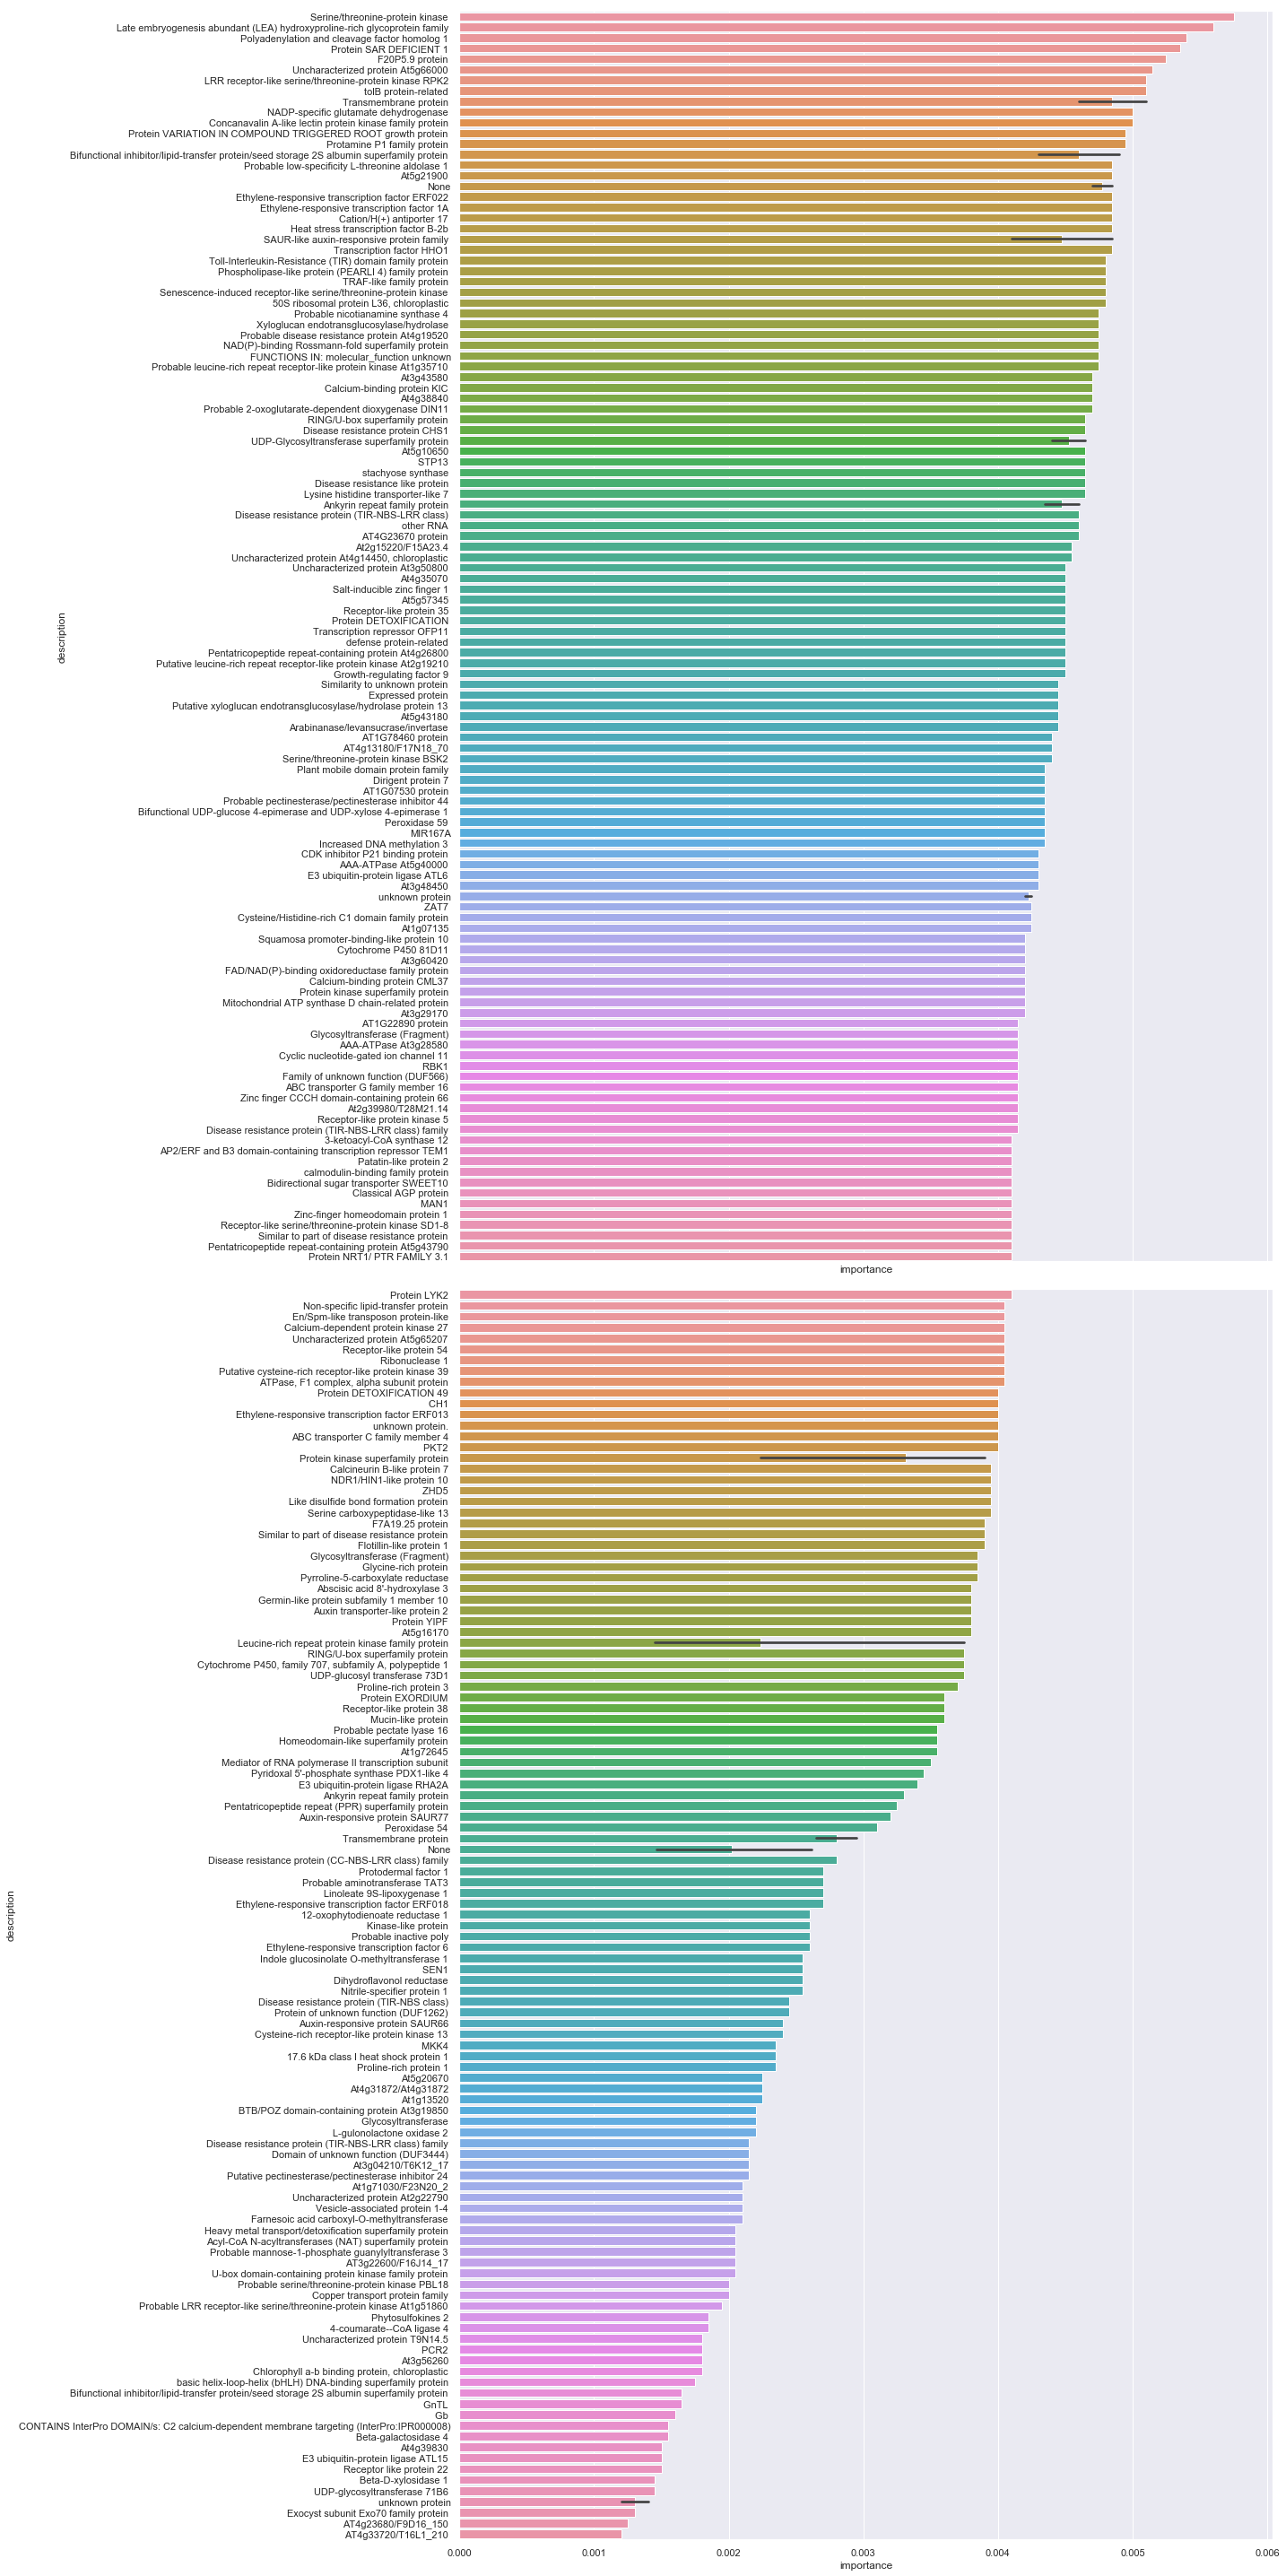
\includegraphics[width=.9\linewidth]{obipy-resources/93e2fbf76ed477962282ae99767b8408de4d3ed9/703f60afdc6ffbfb23a6c0113ee865a2ebf33ef0.png}
\end{center}


\section{Selecting genes for all genotypes at all times C/W}
\label{sec:orgdc8d628}
\subsection{RFE selecting 25 genes}
\label{sec:org6b5cc95}
\begin{minted}[frame=lines,linenos=true,fontfamily=Monaco]{ipython}
from sklearn.feature_selection import RFE, RFECV
from sklearn.linear_model import LogisticRegression

# load data
DE_pairings_05hr = read_xl('/Users/hughesn/PHD/Transcripts/Data/pairings_05hr.xlsx')
sig = DE_pairings_05hr[DE_pairings_05hr['padj'] < 0.01]
sig = sig['log2FoldChange'].sort_values()
locs = sig.index
df = counts.loc[locs][[c for c in counts.columns if (('col' in c or 'lym' in c or 'cer' in c))]].T
df = df.loc[:,~df.columns.duplicated()]
df = df[[c for c in set(df.columns.values)]]
\end{minted}

\begin{minted}[frame=lines,linenos=true,fontfamily=Monaco]{ipython}
# Feature Extraction with RFE
X = df.values
y = [y.rsplit('_',1)[0] for y in df.reset_index()['index']]
# feature extraction
model = LogisticRegression()
rfe = RFE(model, n_features_to_select=25)
fit = rfe.fit(X, y)
print("Num Features: {0}".format(fit.n_features_))
print("Selected Features: {0}".format(fit.support_))
print("Feature Ranking: {0}".format(fit.ranking_))
\end{minted}

Num Features: 25\\
Selected Features: [False False False \ldots{} False False False]\\
Feature Ranking: [ 821 2397 3365 \ldots{}  912  633 1129]\\


\begin{minted}[frame=lines,linenos=true,fontfamily=Monaco]{ipython}
genes = []
for r,f in zip(fit.ranking_, df.columns.values):
      if r ==1:
            genes.append(f)
get_gene_names(genes)
\end{minted}

\begin{center}
\begin{tabular}{rlll}
 & incoming & name & description\\
\hline
0 & AT3G06355 & AT3G06355 & None\\
1 & AT4G29780 & AT4G29780 & Nuclease\\
2 & AT1G62730 & AT1G62730 & At1g62730\\
3 & AT1G26380 & FOX1 & Berberine bridge enzyme-like 3\\
4 & AT1G62740 & HOP2 & Hsp70-Hsp90 organizing protein 2\\
5 & AT5G24110 & WRKY30 & Probable WRKY transcription factor 30\\
6 & AT5G63160 & BT1 & BTB/POZ and TAZ domain-containing protein 1\\
7 & AT3G47420 & ATPS3 & Putative glycerol-3-phosphate transporter 1\\
8 & AT3G28740 & CYP81D11 & Cytochrome P450 81D11\\
9 & AT4G08950 & EXO & Protein EXORDIUM\\
10 & AT4G24570 & PUMP4 & DIC2\\
11 & AT4G35180 & LHT7 & Lysine histidine transporter-like 7\\
12 & AT5G20620 & UBQ4 & Polyubiquitin 4\\
13 & AT4G23680 & AT4G23680 & AT4g23680/F9D16\_150\\
14 & AT1G24280 & G6PD3 & Glucose-6-phosphate 1-dehydrogenase\\
15 & AT3G09440 & HSP70-3 & Heat shock protein 70 (Hsp 70) family protein\\
16 & AT3G50770 & CML41 & Probable calcium-binding protein CML41\\
17 & AT1G02930 & GSTF6 & Glutathione S-transferase F6\\
18 & AT1G56660 & AT1G56660 & F25P12.91 protein\\
19 & AT1G26240 & AT1G26240 & Proline-rich extensin-like family protein\\
20 & AT5G49360 & BXL1 & Beta-D-xylosidase 1\\
21 & AT3G44860 & FAMT & Farnesoic acid carboxyl-O-methyltransferase\\
22 & AT4G24110 & AT4G24110 & NADP-specific glutamate dehydrogenase\\
23 & AT2G17120 & LYM2 & LysM domain-containing GPI-anchored protein 2\\
24 & AT5G21940 & AT5G21940 & At5g21940\\
\end{tabular}
\end{center}


\subsubsection{Forest on this RFE set}
\label{sec:org7ad30ee}

\begin{minted}[frame=lines,linenos=true,fontfamily=Monaco]{ipython}
rfe_forest = counts.loc[genes][[c for c in counts.columns if ('col' in c or 'lym' in c or 'cer' in c)]].T
rfe_forest = rfe_forest.loc[:,~rfe_forest.columns.duplicated()]
rfe_forest = rfe_forest[[c for c in set(rfe_forest.columns.values)]]

feat_labels = rfe_forest.columns.values
y = [d.rsplit('_', 1)[0] for d in rfe_forest.index.values]

X_train, X_test, y_train, y_test = train_test_split(rfe_forest.values, y, test_size=1, random_state=42)
forest = RandomForestClassifier(n_estimators=200000, random_state=1, n_jobs=-1)
forest.fit(X_train, y_train)
res = {k: v for k, v in sorted(
    zip(feat_labels, forest.feature_importances_), key=lambda x: x[1], reverse=True)}
res_df = pd.DataFrame(list(res.items()), columns=[
                      'gene', 'importance']).set_index('gene')
names = get_gene_names(list(res_df.index))
res_df = pd.merge(res_df, names, left_index=True, right_on='incoming').rename(
    columns={'incoming': 'gene'}).set_index('gene').sort_values('importance', ascending=False)
res_df
\end{minted}

\begin{center}
\begin{tabular}{lrll}
gene & importance & name & description\\
\hline
AT5G20620 & 0.0594945 & UBQ4 & Polyubiquitin 4\\
AT4G08950 & 0.0537744 & EXO & Protein EXORDIUM\\
AT3G06355 & 0.0523862 & AT3G06355 & None\\
AT4G24110 & 0.0504935 & AT4G24110 & NADP-specific glutamate dehydrogenase\\
AT3G28740 & 0.0501161 & CYP81D11 & Cytochrome P450 81D11\\
AT5G21940 & 0.0498109 & AT5G21940 & At5g21940\\
AT3G09440 & 0.0491729 & HSP70-3 & Heat shock protein 70 (Hsp 70) family protein\\
AT1G02930 & 0.0476493 & GSTF6 & Glutathione S-transferase F6\\
AT5G63160 & 0.0449373 & BT1 & BTB/POZ and TAZ domain-containing protein 1\\
AT1G24280 & 0.044786 & G6PD3 & Glucose-6-phosphate 1-dehydrogenase\\
AT2G17120 & 0.0421376 & LYM2 & LysM domain-containing GPI-anchored protein 2\\
AT3G50770 & 0.0421243 & CML41 & Probable calcium-binding protein CML41\\
AT5G49360 & 0.0420693 & BXL1 & Beta-D-xylosidase 1\\
AT1G62740 & 0.0402053 & HOP2 & Hsp70-Hsp90 organizing protein 2\\
AT4G35180 & 0.0390995 & LHT7 & Lysine histidine transporter-like 7\\
AT4G29780 & 0.0351811 & AT4G29780 & Nuclease\\
AT3G47420 & 0.0334156 & ATPS3 & Putative glycerol-3-phosphate transporter 1\\
AT1G62730 & 0.0328065 & AT1G62730 & At1g62730\\
AT1G26380 & 0.0322609 & FOX1 & Berberine bridge enzyme-like 3\\
AT4G24570 & 0.0316438 & PUMP4 & DIC2\\
AT1G56660 & 0.0296291 & AT1G56660 & F25P12.91 protein\\
AT1G26240 & 0.0285743 & AT1G26240 & Proline-rich extensin-like family protein\\
AT5G24110 & 0.0250461 & WRKY30 & Probable WRKY transcription factor 30\\
AT3G44860 & 0.022443 & FAMT & Farnesoic acid carboxyl-O-methyltransferase\\
AT4G23680 & 0.0207426 & AT4G23680 & AT4g23680/F9D16\_150\\
\end{tabular}
\end{center}


\begin{minted}[frame=lines,linenos=true,fontfamily=Monaco]{ipython}
fig, ax = plt.subplots(1, figsize=(20,20))
sns.barplot(data=res_df.reset_index(), y='description', x='importance', ax=ax)
plt.tight_layout()
\end{minted}

\begin{verbatim}
<Figure size 1440x1440 with 1 Axes>
\end{verbatim}


\begin{center}
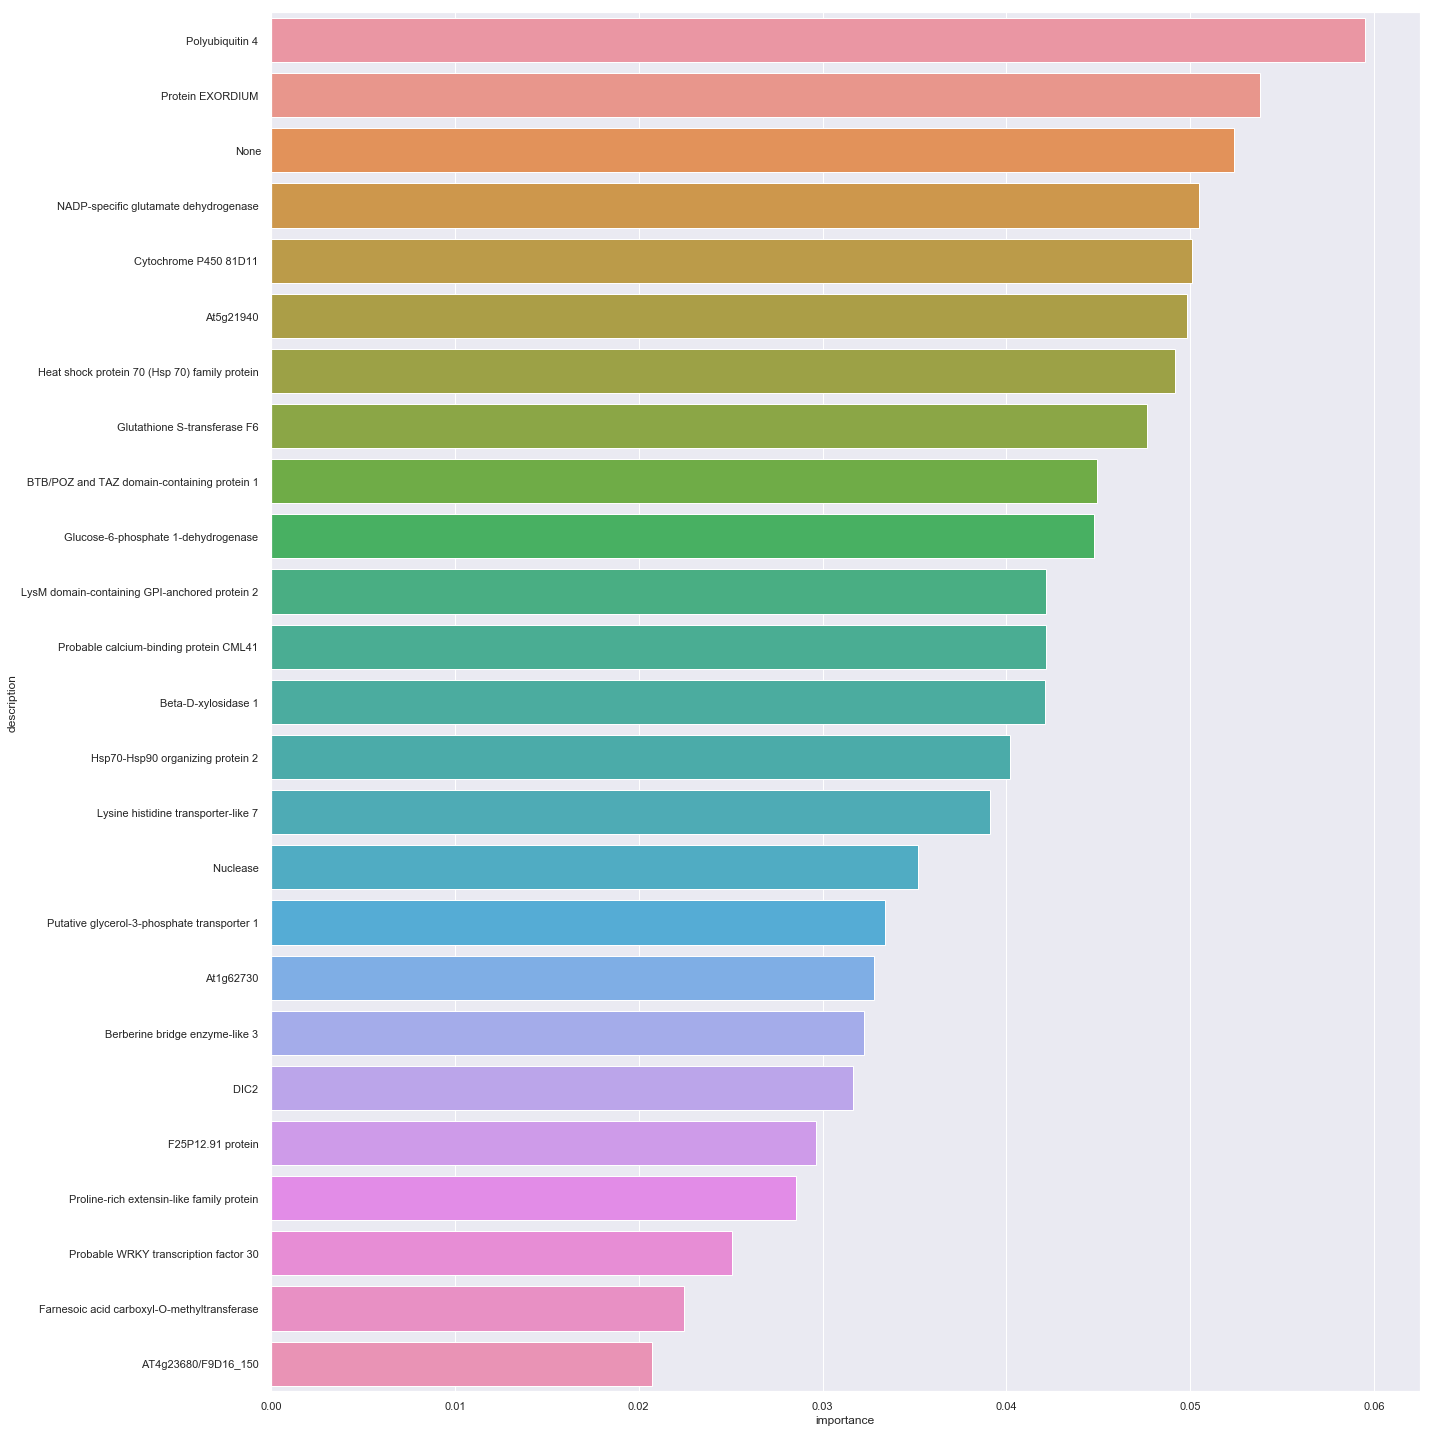
\includegraphics[width=.9\linewidth]{obipy-resources/93e2fbf76ed477962282ae99767b8408de4d3ed9/65666fbca873a47968edcf553fd409812446c3ba.png}
\end{center}




\paragraph{C45 Decision tree}
\label{sec:orgc386f35}

\begin{minted}[frame=lines,linenos=true,fontfamily=Monaco]{ipython}
from sklearn.tree import DecisionTreeClassifier
rfe_forest = counts.loc[genes][[c for c in counts.columns if ('col' in c or 'lym' in c or 'cer' in c)]].T
rfe_forest = rfe_forest.loc[:,~rfe_forest.columns.duplicated()]
rfe_forest = rfe_forest[[c for c in set(rfe_forest.columns.values)]]

feat_labels = rfe_forest.columns.values
y = [d.rsplit('_', 1)[0] for d in rfe_forest.index.values]

X_train, X_test, y_train, y_test = train_test_split(rfe_forest.values, y, test_size=1, random_state=42)
gnb = DecisionTreeClassifier()
gnb = gnb.fit(X_train, y_train)

# Export as dot file
export_graphviz(gnb, out_file='./tree.dot',
                feature_names = get_gene_names(list(feat_labels))['description'].values,
                class_names = list(set(y)),
                rounded = True, proportion = False,
                precision = 2, filled = True)
# Convert to png using system command (requires Graphviz)
from subprocess import call
_=call(['dot', '-Tpng', './tree.dot', '-o', './tree.png', '-Gdpi=50'])
print('[[./tree.png]]')

\end{minted}

NameErrorTraceback (most recent call last)\\
<ipython-input-188-da840864ae98> in <module>\\
     12\\
     13 \# Export as dot file\\
---> 14 export\_graphviz(gnb, out\_file='./tree.dot',\\
     15                 feature\_names = get\_gene\_names(list(feat\_labels))['description'].values,\\
     16                 class\_names = list(set(y)),\\

NameError: name 'export\_graphviz' is not defined\\
\section{Test hypotheses}
\label{sec:org56e16dd}

\begin{itemize}
\item \emph{There are no differences in water treatments at 05hr for..}\\
\begin{itemize}
\item \emph{Col0 and Cerk1}\\
\item \emph{Col0 and Lym2}\\
\item \emph{Cerk1 and Lym2}\\
\end{itemize}

\item \emph{There are no differences in chitin treatments at 05hr for..}\\
\begin{itemize}
\item \emph{Col0 and Cerk1}\\
\item \emph{Col0 and Lym2}\\
\item \emph{Cerk1 and Lym2}\\
\end{itemize}

\item \emph{There are no differences in water treatments at 6hr for..}\\
\begin{itemize}
\item \emph{Col0 and Cerk1}\\
\item \emph{Col0 and Lym2}\\
\item \emph{Cerk1 and Lym2}\\
\end{itemize}

\item \emph{There are no differences in chitin treatments at 6hr for..}\\
\begin{itemize}
\item \emph{Col0 and Cerk1}\\
\item \emph{Col0 and Lym2}\\
\item \emph{Cerk1 and Lym2}\\
\end{itemize}
\end{itemize}


\subsection{Are there differences at 05hr}
\label{sec:org0cb6667}


\subsubsection{In Water-water and chitin-chitin treatments?}
\label{sec:orga54dd1b}


\begin{minted}[frame=lines,linenos=true,fontfamily=Monaco]{ipython}
DE_pairings_w_05hr = read_xl('/Users/hughesn/PHD/Transcripts/Data/pairings_same_treat_05hr.xlsx', unique=False)
\end{minted}

\begin{verbatim}
<Figure size 360x360 with 1 Axes>
\end{verbatim}


\begin{figure}[htbp]
\centering
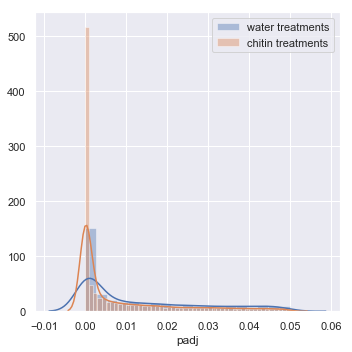
\includegraphics[width=15cm]{obipy-resources/test_water.png.png}
\caption{\label{test_water.png}
Are there differences in water treatments?}
\end{figure}


\begin{verbatim}
<Figure size 432x288 with 1 Axes>
\end{verbatim}


\begin{figure}[htbp]
\centering
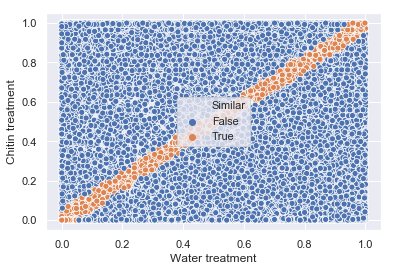
\includegraphics[width=15cm]{obipy-resources/scatter_genes_water_v_chitin.png}
\caption{\label{scatter_genes_water_v_chitin}
DE genes are different in water / chitin}
\end{figure}




\subsubsection{In Chitin and water treatments, across samples?}
\label{sec:org3ed39a1}


\begin{minted}[frame=lines,linenos=true,fontfamily=Monaco]{ipython}
DE_pairings_c_05hr = read_xl('/Users/hughesn/PHD/Transcripts/Data/pairings_05hr.xlsx', unique=True)
\end{minted}

\begin{verbatim}
<Figure size 1224x1008 with 6 Axes>
\end{verbatim}


\begin{figure}[htbp]
\centering
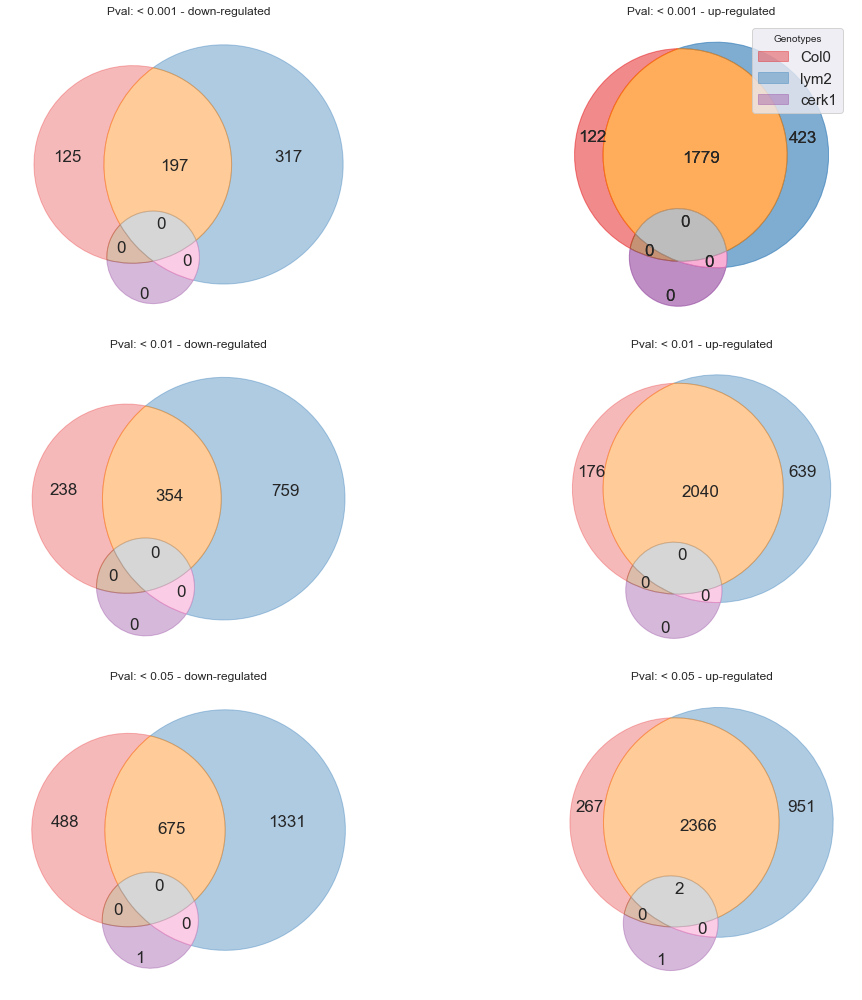
\includegraphics[width=10cm]{obipy-resources/vennTreatmentschitin.png}
\caption{\label{vennTreatments}
Venn diagram hypothesis of the chitin effect}
\end{figure}








\paragraph{Overlapping genes for Col and Lym at 05hr W/C treatments}
\label{sec:org3459087}
\begin{center}
\begin{tabular}{rlll}
 & incoming & name & description\\
\hline
0 & AT5G45110 & NPR3 & NPR3\\
1 & AT5G15130 & WRKY72 & Probable WRKY transcription factor 72\\
2 & AT3G04110 & GLR1.1 & Glutamate receptor 1.1\\
3 & AT3G15530 & AT3G15530 & Expressed protein\\
4 & AT5G44568 & AT5G44568 & Transmembrane protein\\
5 & AT5G44190 & GLK2 & Transcription activator GLK2\\
6 & AT1G08050 & AT1G08050 & T6D22.13\\
7 & AT2G44380 & AT2G44380 & At2g44380\\
8 & AT5G43760 & KCS20 & 3-ketoacyl-CoA synthase\\
9 & AT2G20960 & pEARLI4 & PEARLI 4 protein\\
10 & AT1G47130 & AT1G47130 & None\\
11 & AT1G69840 & HIR2 & Hypersensitive-induced response protein 2\\
12 & AT1G43000 & AT1G43000 & PLATZ transcription factor family protein\\
13 & AT4G23250 & EMB1290 & kinases\\
14 & AT2G46400 & WRKY46 & Probable WRKY transcription factor 46\\
15 & AT2G02180 & TOM3 & Tobamovirus multiplication protein 3\\
16 & AT1G72430 & SAUR78 & Auxin-responsive protein SAUR78\\
17 & AT5G52670 & AT5G52670 & Copper transport protein family\\
18 & AT3G17770 & AT3G17770 & At3g17770\\
19 & AT5G00990 & AT5G00990 & None\\
20 & AT3G11810 & AT3G11810 & F26K24.10 protein\\
21 & AT1G10040 & AT1G10040 & Alpha/beta-Hydrolases superfamily protein\\
22 & AT1G50040 & AT1G50040 & F2J10.8 protein\\
23 & AT2G35710 & PGSIP8 & Putative glucuronosyltransferase PGSIP8\\
24 & AT2G18685 & AT2G18685 & None\\
25 & AT1G67310 & CAMTA4 & Calmodulin-binding transcription activator 4\\
26 & AT3G52710 & AT3G52710 & Uncharacterized protein At3g52710\\
27 & AT1G13530 & AT1G13530 & Protein of unknown function (DUF1262)\\
28 & AT4G15800 & RALFL33 & Protein RALF-like 33\\
29 & AT1G74100 & SOT16 & Sulfotransferase\\
30 & AT4G08500 & MEKK1 & Mitogen-activated protein kinase kinase kinase 1\\
31 & AT3G14870 & AT3G14870 & AT3G14870 protein\\
32 & AT3G12610 & DRT100 & DRT100\\
33 & AT1G69930 & GSTU11 & Glutathione S-transferase U11\\
34 & AT1G67460 & AT1G67460 & None\\
35 & AT5G23130 & AT5G23130 & Peptidoglycan-binding LysM domain-containing protein\\
36 & AT5G58940 & CRCK1 & Calmodulin-binding receptor-like cytoplasmic kinase 1\\
37 & AT3G15810 & AT3G15810 & Protein LURP-one-related 12\\
38 & AT4G39830 & AT4G39830 & At4g39830\\
39 & AT1G53170 & ERF8 & Ethylene-responsive transcription factor 8\\
40 & AT1G24020 & MLP423 & MLP-like protein 423\\
41 & AT2G41890 & SD31 & G-type lectin S-receptor-like serine/threonine-protein kinase SD3-1\\
42 & AT5G05995 & AT5G05995 & None\\
43 & AT5G67250 & SKIP2 & F-box protein SKIP2\\
44 & AT1G30740 & AT1G30740 & FAD-binding Berberine family protein\\
45 & AT3G07565 & AT3G07565 & Histone H2A deubiquitinase (DUF3755)\\
46 & AT1G70530 & CRK3 & Cysteine-rich receptor-like protein kinase 3\\
47 & AT1G63360 & AT1G63360 & Probable disease resistance protein At1g63360\\
48 & AT5G01732 & AT5G01732 & other RNA\\
49 & AT2G41100 & CML12 & Calmodulin-like protein 12\\
50 & AT5G18500 & AT5G18500 & Probable receptor-like protein kinase At5g18500\\
51 & AT1G08315 & AT1G08315 & ARM repeat superfamily protein\\
52 & AT3G44720 & ADT4 & Arogenate dehydratase 4, chloroplastic\\
53 & AT5G03320 & PCRK2 & Serine/threonine-protein kinase PCRK2\\
54 & AT4G24580 & REN1 & Rho GTPase-activating protein REN1\\
55 & AT1G70230 & AXY4 & TBL27\\
56 & AT3G63450 & AT3G63450 & RNA-binding (RRM/RBD/RNP motifs) family protein\\
57 & AT5G45090 & PP2A7 & Uncharacterized protein PHLOEM PROTEIN 2-LIKE A7\\
58 & AT1G18890 & CPK10 & Calcium-dependent protein kinase 10\\
59 & AT4G26090 & RPS2 & Disease resistance protein RPS2\\
60 & AT4G20000 & AT4G20000 & At4g20000\\
61 & AT1G79110 & BRG2 & Probable BOI-related E3 ubiquitin-protein ligase 2\\
62 & AT5G57770 & AT5G57770 & Plant protein of unknown function (DUF828) with plant pleckstrin homology-like region\\
63 & AT1G21010 & AT1G21010 & At1g21010\\
64 & AT4G11890 & AT4G11890 & Protein kinase superfamily protein\\
65 & AT1G55365 & AT1G55365 & Putative uncharacterized protein\\
66 & AT3G27560 & ATN1 & AT3g27560/MMJ24\_11\\
67 & AT1G07130 & STN1 & CST complex subunit STN1\\
68 & AT5G15850 & COL1 & Zinc finger protein CONSTANS-LIKE 1\\
69 & AT1G22930 & AT1G22930 & T-complex protein 11\\
70 & AT1G11670 & DTX36 & Protein DETOXIFICATION 36\\
71 & AT4G24920 & AT4G24920 & secE/sec61-gamma protein transport protein\\
72 & AT4G17500 & ERF1A & Ethylene-responsive transcription factor 1A\\
73 & AT4G04435 & AT4G04435 & None\\
74 & AT2G15042 & AT2G15042 & Leucine-rich repeat (LRR) family protein\\
75 & AT1G56140 & AT1G56140 & Probable LRR receptor-like serine/threonine-protein kinase At1g56140\\
76 & AT1G77240 & AEE4 & AAE2\\
77 & AT4G29050 & AT4G29050 & Concanavalin A-like lectin protein kinase family protein\\
78 & AT4G19510 & AT4G19510 & Disease resistance protein (TIR-NBS-LRR class)\\
79 & AT1G17255 & AT1G17255 & other RNA\\
80 & AT1G61562 & AT1G61562 & None\\
81 & AT1G22510 & AT1G22510 & E3 ubiquitin-protein ligase RNF170-like protein (DUF 1232)\\
82 & AT1G17860 & KTI2 & Kunitz trypsin inhibitor 2\\
83 & AT2G14910 & AT2G14910 & MAR-binding filament-like protein\\
84 & AT1G31290 & AGO3 & Protein argonaute 3\\
85 & AT2G34520 & RPS14 & At2g34520\\
86 & AT4G01950 & ATGPAT3 & glycerol-3-phosphate acyltransferase 3\\
87 & AT5G25920 & AT5G25920 & BEST Arabidopsis thaliana protein match is: Eukaryotic aspartyl protease family protein (TAIR:AT3G29750.1)\\
88 & AT3G44480 & RPP1 & Disease resistance protein (TIR-NBS-LRR class) family\\
89 & AT5G51190 & ERF105 & Ethylene-responsive transcription factor ERF105\\
90 & AT3G56790 & AT3G56790 & RNA splicing factor-like protein\\
91 & AT2G32030 & AT2G32030 & Acyl-CoA N-acyltransferases (NAT) superfamily protein\\
92 & AT5G54490 & PBP1 & PBP1\\
93 & AT3G10985 & SAG20 & Senescence associated gene 20\\
94 & AT1G42470 & AT1G42470 & Patched family protein\\
95 & AT5G08790 & NAC081 & Protein ATAF2\\
96 & AT1G67810 & SUFE2 & SufE-like protein 2, chloroplastic\\
97 & AT4G24160 & AT4G24160 & 1-acylglycerol-3-phosphate O-acyltransferase\\
98 & AT2G42350 & ATL40 & RING-H2 finger protein ATL40\\
99 & AT4G30910 & AT4G30910 & Cytosol aminopeptidase family protein\\
100 & AT1G74930 & ERF018 & Ethylene-responsive transcription factor ERF018\\
101 & AT3G60630 & SCL22 & Scarecrow-like protein 22\\
102 & AT1G70170 & 2MMP & Metalloendoproteinase 2-MMP\\
103 & AT3G30180 & CYP85A2 & Cytochrome P450 85A2\\
104 & AT4G32300 & SD25 & G-type lectin S-receptor-like serine/threonine-protein kinase SD2-5\\
105 & AT1G59970 & 5MMP & Metalloendoproteinase 5-MMP\\
106 & AT1G65690 & NHL6 & NDR1/HIN1-like protein 6\\
107 & AT1G67880 & AT1G67880 & Beta-1,4-N-acetylglucosaminyltransferase family protein\\
108 & AT1G18160 & AT1G18160 & Protein kinase superfamily protein\\
109 & AT4G23220 & CRK14 & Cysteine-rich receptor-like protein kinase 14\\
110 & AT4G35310 & CPK5 & CPK5\\
111 & AT2G45160 & SCL27 & Scarecrow-like protein 27\\
112 & AT2G21900 & WRKY59 & At2g21900\\
113 & AT5G22060 & ATJ2 & At5g22060\\
114 & AT1G63680 & ATMURE & UDP-N-acetylmuramoyl-L-alanyl-D-glutamate--2,6-diaminopimelate ligase MurE homolog, chloroplastic\\
115 & AT2G40095 & AT2G40095 & Alpha/beta hydrolase related protein\\
116 & AT5G59820 & ZAT12 & Zinc finger protein ZAT12\\
117 & AT4G36670 & PLT6 & At4g36670\\
118 & AT3G02770 & AT3G02770 & Putative 4-hydroxy-4-methyl-2-oxoglutarate aldolase 1\\
119 & AT2G38470 & WRKY33 & WRKY33\\
120 & AT3G57330 & ACA11 & Putative calcium-transporting ATPase 11, plasma membrane-type\\
121 & AT1G60505 & AT1G60505 & other RNA\\
122 & AT2G38780 & AT2G38780 & unknown protein\\
123 & AT1G06135 & AT1G06135 & Transmembrane protein\\
124 & AT4G31950 & CYP82C3 & CYP82C3\\
125 & AT5G53550 & YSL3 & YSL3\\
126 & AT1G16090 & WAKL7 & Wall associated kinase-like 7\\
127 & AT1G61470 & CAF1-5 & Probable CCR4-associated factor 1 homolog 5\\
128 & AT1G20510 & 4CLL5 & 4-coumarate--CoA ligase-like 5\\
129 & AT3G25240 & AT3G25240 & Sulfate/thiosulfate import ATP-binding protein, putative (DUF506)\\
130 & AT1G49205 & AT1G49205 & None\\
131 & AT3G06870 & AT3G06870 & Proline-rich family protein\\
132 & AT1G72700 & ALA5 & Probable phospholipid-transporting ATPase 5\\
133 & AT4G36990 & HSFB1 & Heat stress transcription factor B-1\\
134 & AT5G11000 & AT5G11000 & AT5g11000/T30N20\_270\\
135 & AT4G29780 & AT4G29780 & Nuclease\\
136 & AT1G01560 & MPK11 & Mitogen-activated protein kinase 11\\
137 & AT5G24380 & YSL2 & Metal-nicotianamine transporter YSL2\\
138 & AT5G05250 & AT5G05250 & AT5g05250/K18I23\_5\\
139 & AT5G48400 & GLR1.2 & Glutamate receptor 1.2\\
140 & AT4G23810 & WRKY53 & Probable WRKY transcription factor 53\\
141 & AT1G26420 & FOX5 & Berberine bridge enzyme-like 7\\
142 & AT3G05320 & OFUT23 & O-fucosyltransferase 23\\
143 & AT1G30040 & GA2OX2 & Gibberellin 2-beta-dioxygenase 2\\
144 & AT2G29340 & AT2G29340 & Tropinone reductase homolog At2g29340\\
145 & AT1G14280 & PKS2 & Protein PHYTOCHROME KINASE SUBSTRATE 2\\
146 & AT2G03530 & UPS2 & ureide permease 2\\
147 & AT3G57880 & AT3G57880 & Anthranilate phosphoribosyltransferase-like protein\\
148 & AT3G53600 & AT3G53600 & At3g53600\\
149 & AT2G41105 & AT2G41105 & None\\
150 & AT5G48880 & KAT5 & PKT2\\
151 & AT1G06983 & AT1G06983 & None\\
152 & AT3G29075 & AT3G29075 & Glycine-rich protein\\
153 & AT1G19270 & DA1 & DA1\\
154 & AT2G08895 & AT2G08895 & None\\
155 & AT2G35935 & AT2G35935 & None\\
156 & AT4G26400 & AT4G26400 & AT4G26400 protein\\
157 & AT5G12340 & AT5G12340 & DUF4228 domain protein\\
158 & AT1G11210 & AT1G11210 & At1g11210/T28P6\_5\\
159 & AT5G07080 & AT5G07080 & HXXXD-type acyl-transferase family protein\\
160 & AT3G27880 & AT3G27880 & At3g27880\\
161 & AT1G30720 & AT1G30720 & Berberine bridge enzyme-like 10\\
162 & AT3G09010 & AT3G09010 & Protein kinase superfamily protein\\
163 & AT5G58750 & AT5G58750 & At5g58750\\
164 & AT5G13180 & NAC083 & NAC domain-containing protein 83\\
165 & AT4G19920 & AT4G19920 & Toll-Interleukin-Resistance (TIR) domain family protein\\
166 & AT2G30720 & AT2G30720 & At2g30720\\
167 & AT1G64610 & AT1G64610 & Transducin/WD40 repeat-like superfamily protein\\
168 & AT5G66310 & KIN7H & Kinesin-like protein KIN-7H\\
169 & AT5G54500 & FQR1 & Flavodoxin-like quinone reductase 1\\
170 & AT5G54730 & ATG18F & Autophagy-related protein 18f\\
171 & AT5G11250 & AT5G11250 & Disease resistance protein (TIR-NBS-LRR class)\\
172 & AT1G72790 & AT1G72790 & Hydroxyproline-rich glycoprotein family protein\\
173 & AT4G18205 & PUP22 & Probable purine permease 22\\
174 & AT1G27770 & ACA1 & Calcium-transporting ATPase\\
175 & AT1G61660 & BHLH112 & Transcription factor bHLH112\\
176 & AT1G53430 & AT1G53430 & Probable LRR receptor-like serine/threonine-protein kinase At1g53430\\
177 & AT1G18980 & AT1G18980 & At1g18980\\
178 & AT2G41730 & AT2G41730 & Calcium-binding site protein\\
179 & AT3G12920 & BRG3 & Probable BOI-related E3 ubiquitin-protein ligase 3\\
180 & AT1G02390 & GPAT2 & Probable glycerol-3-phosphate acyltransferase 2\\
181 & AT2G44010 & AT2G44010 & At2g44010\\
182 & AT4G25670 & AT4G25670 & AT4g25670/L73G19\_50\\
183 & AT2G47190 & ATMYB2 & ATMYB2\\
184 & AT2G28210 & ATACA2 & ATACA2\\
185 & AT1G09903 & AT1G09903 & None\\
186 & AT4G36648 & AT4G36648 & other RNA\\
187 & AT1G79670 & WAKL22 & WAKL22\\
188 & AT3G56050 & AT3G56050 & Probable inactive receptor-like protein kinase At3g56050\\
189 & AT1G61140 & EDA16 & SNF2 domain-containing protein / helicase domain-containing protein / zinc finger protein-like protein\\
190 & AT4G35720 & AT4G35720 & DUF241 domain protein, putative (DUF241)\\
191 & AT1G29160 & DOF1.5 & Uncharacterized protein At1g29160 (Fragment)\\
192 & AT4G35985 & P85 & Senescence/dehydration-associated protein At4g35985, chloroplastic\\
193 & AT4G22780 & ACR7 & ACT domain-containing protein ACR7\\
194 & AT4G30720 & AT4G30720 & FAD/NAD(P)-binding oxidoreductase family protein\\
195 & AT2G19710 & AT2G19710 & Regulator of Vps4 activity in the MVB pathway protein\\
196 & AT1G18210 & CML27 & Probable calcium-binding protein CML27\\
197 & AT1G51920 & AT1G51920 & unknown protein\\
198 & AT3G53400 & AT3G53400 & Peptide upstream protein\\
199 & AT2G43000 & JUB1 & Transcription factor JUNGBRUNNEN 1\\
200 & AT2G02800 & PBL3 & Probable serine/threonine-protein kinase PBL3\\
201 & AT5G52530 & AT5G52530 & Dentin sialophosphoprotein-like protein\\
202 & AT3G06760 & AT3G06760 & Drought-responsive family protein\\
203 & AT3G46090 & ZAT7 & ZAT7\\
204 & AT4G27652 & AT4G27652 & At4g27652\\
205 & AT4G11530 & CRK34 & cysteine-rich RLK (RECEPTOR-like protein kinase) 34\\
206 & AT5G44990 & AT5G44990 & Glutathione S-transferase family protein\\
207 & AT1G10470 & ARR4 & Two-component response regulator ARR4\\
208 & AT1G78895 & RTNLB22 & Reticulon-like protein B22\\
209 & AT1G73730 & EIL3 & SLIM1\\
210 & AT3G05670 & AT3G05670 & F18C1.6 protein\\
211 & AT2G23450 & WAKL14 & Wall-associated receptor kinase-like 14\\
212 & AT1G64380 & ERF061 & Ethylene-responsive transcription factor ERF061\\
213 & AT5G49520 & WRKY48 & Probable WRKY transcription factor 48\\
214 & AT3G28180 & CSLC4 & Glycosyltransferase (Fragment)\\
215 & AT3G07390 & AIR12 & AIR12\\
216 & AT5G59490 & AT5G59490 & At5g59490\\
217 & AT2G35000 & ATL9 & E3 ubiquitin-protein ligase ATL9\\
218 & AT3G53150 & UGT73D1 & UDP-glucosyl transferase 73D1\\
219 & AT5G08870 & AT5G08870 & None\\
220 & AT5G64890 & PEP2 & Elicitor peptide 2\\
221 & AT4G24230 & ACBP3 & Acyl-CoA-binding domain 3\\
222 & AT3G11410 & PP2CA & Protein phosphatase 2C 37\\
223 & AT3G25600 & CML16 & Probable calcium-binding protein CML16\\
224 & AT2G36650 & AT2G36650 & CHUP1-like protein\\
225 & AT1G19330 & AT1G19330 & unknown protein\\
226 & AT5G35735 & AT5G35735 & Cytochrome b561 and DOMON domain-containing protein At5g35735\\
227 & AT1G51620 & AT1G51620 & Protein kinase superfamily protein\\
228 & AT4G02420 & LECRK44 & L-type lectin-domain containing receptor kinase IV.4\\
229 & AT1G34245 & EPF2 & EPF2\\
230 & AT5G02895 & AT5G02895 & None\\
231 & AT4G16957 & AT4G16957 & SUPPRESSOR OF, CONSTITUTIVE protein\\
232 & AT3G50830 & COR413PM2 & COR413-PM2\\
233 & AT3G09520 & ATEXO70H4 & Exocyst subunit Exo70 family protein\\
234 & AT5G01550 & LECRKA4.2 & lectin receptor kinase a4.1\\
235 & AT3G46930 & AT3G46930 & Protein kinase superfamily protein\\
236 & AT2G20950 & AT2G20950 & Arabidopsis phospholipase-like protein (PEARLI 4) family\\
237 & AT1G67510 & AT1G67510 & Leucine-rich repeat protein kinase family protein\\
238 & AT5G35370 & AT5G35370 & G-type lectin S-receptor-like serine/threonine-protein kinase At5g35370\\
239 & AT3G59880 & AT3G59880 & Expressed protein\\
240 & AT3G56800 & CAM5 & Calmodulin-2\\
241 & AT3G10525 & SMR1 & SMR1\\
242 & AT1G58110 & AT1G58110 & Basic-leucine zipper (BZIP) transcription factor family protein\\
243 & AT5G47720 & AT5G47720 & AACT1\\
244 & AT2G15220 & AT2G15220 & At2g15220/F15A23.4\\
245 & AT3G50470 & HR3 & MLA10\\
246 & AT2G39210 & AT2G39210 & At2g39210/T16B24.15\\
247 & AT5G44290 & AT5G44290 & AT5G44290 protein\\
248 & AT1G15800 & AT1G15800 & At1g15800\\
249 & AT4G39030 & DTX47 & Protein DETOXIFICATION 47, chloroplastic\\
250 & AT4G23015 & AT4G23015 & Transmembrane protein\\
251 & AT3G13600 & IQM2 & Calmodulin-binding family protein\\
252 & AT2G42010 & PLDBETA1 & phospholipase D beta 1\\
253 & AT3G45210 & AT3G45210 & AT3g45210/T14D3\_150\\
254 & AT2G46620 & AT2G46620 & AAA-ATPase At2g46620\\
255 & AT5G65200 & PUB38 & U-box domain-containing protein 38\\
256 & AT4G23140 & CRK6 & cysteine-rich RLK (RECEPTOR-like protein kinase) 6\\
257 & AT3G19030 & AT3G19030 & AT3g19030/K13E13\_15\\
258 & AT2G32240 & AT2G32240 & FUNCTIONS IN: molecular\_function unknown\\
259 & AT4G22467 & AT4G22467 & None\\
260 & AT2G09440 & AT2G09440 & None\\
261 & AT5G46580 & AT5G46580 & Pentatricopeptide repeat-containing protein At5g46580, chloroplastic\\
262 & AT3G45040 & EVN & Dolichol kinase EVAN\\
263 & AT1G58225 & AT1G58225 & At1g58225\\
264 & AT5G05140 & MED26B & Probable mediator of RNA polymerase II transcription subunit 26b\\
265 & AT3G61640 & AGP20 & Arabinogalactan protein 20\\
266 & AT1G01260 & BHLH13 & Transcription factor bHLH13\\
267 & AT3G08170 & AT3G08170 & None\\
268 & AT3G48780 & LCB2B & Long chain base biosynthesis protein 2b\\
269 & AT2G24610 & ATCNGC14 & cyclic nucleotide-gated channel 14\\
270 & AT5G63370 & CDKG1 & Cyclin-dependent kinase G1\\
271 & AT2G18690 & AT2G18690 & Expressed protein\\
272 & AT4G02540 & AT4G02540 & Cysteine/Histidine-rich C1 domain family protein\\
273 & AT2G26300 & GPA1 & Guanine nucleotide-binding protein alpha-1 subunit\\
274 & AT1G27020 & AT1G27020 & Plant/protein\\
275 & AT1G10650 & AT1G10650 & Putative S-ribonuclease binding protein SBP1\\
276 & AT3G09870 & AT3G09870 & F8A24.8 protein\\
277 & AT1G66160 & PUB20 & U-box domain-containing protein 20\\
278 & AT4G11470 & CRK31 & cysteine-rich RLK (RECEPTOR-like protein kinase) 31\\
279 & AT1G55460 & KIN17 & KIN17-like protein\\
280 & AT1G27930 & AT1G27930 & Probable methyltransferase At1g27930\\
281 & AT4G24240 & WRKY7 & Probable WRKY transcription factor 7\\
282 & AT1G12760 & AT1G12760 & E3 ubiquitin-protein ligase At1g12760\\
283 & AT2G27230 & LHW & LHW\\
284 & AT5G53310 & AT5G53310 & AT5g53310/K19E1\_11\\
285 & AT5G46350 & WRKY8 & WRKY transcription factor 8\\
286 & AT3G22260 & AT3G22260 & At3g22260\\
287 & AT5G10750 & AT5G10750 & At5g10750\\
288 & AT1G59820 & ALA3 & Phospholipid-transporting ATPase\\
289 & AT2G39110 & AT2G39110 & Protein kinase superfamily protein\\
290 & AT1G72940 & AT1G72940 & At1g72940/F3N23\_14\\
291 & AT4G38860 & AT4G38860 & At4g38860\\
292 & AT2G02070 & IDD5 & Protein indeterminate-domain 5, chloroplastic\\
293 & AT4G37670 & NAGS2 & NAGS2\\
294 & AT3G03385 & AT3G03385 & None\\
295 & AT2G21500 & AT2G21500 & At2g21560\\
296 & AT4G28085 & AT4G28085 & Transmembrane protein\\
297 & AT2G39480 & ABCB6 & ABC transporter B family member 6\\
298 & AT2G41630 & TFIIB1 & TFIIB1\\
299 & AT1G11050 & AT1G11050 & Probable receptor-like protein kinase At1g11050\\
300 & AT1G01470 & LEA14 & LSR3\\
301 & AT5G37260 & RVE2 & Protein REVEILLE 2\\
302 & AT4G08985 & AT4G08985 & None\\
303 & AT1G11700 & AT1G11700 & At1g11700\\
304 & AT1G71970 & AT1G71970 & At1g71970/F17M19\_12\\
305 & AT5G16830 & SYP21 & Syntaxin-21\\
306 & AT3G19010 & AT3G19010 & 2-oxoglutarate (2OG) and Fe(II)-dependent oxygenase superfamily protein\\
307 & AT2G41110 & CAM2 & Calmodulin 2\\
308 & AT2G48010 & RKF3 & Probable LRR receptor-like serine/threonine-protein kinase RKF3\\
309 & AT2G19130 & AT2G19130 & G-type lectin S-receptor-like serine/threonine-protein kinase At2g19130\\
310 & AT1G11960 & AT1G11960 & Hyperosmolality-gated Ca2+ permeable channel 1.3\\
311 & AT5G58787 & AT5G58787 & RING/U-box superfamily protein\\
312 & AT2G37110 & AT2G37110 & At2g37110\\
313 & AT1G67030 & ZFP6 & Zinc finger protein 6\\
314 & AT4G18253 & AT4G18253 & Receptor Serine/Threonine kinase-like protein\\
315 & AT5G57580 & CBP60B & Calmodulin-binding protein 60 B\\
316 & AT3G22970 & AT3G22970 & At3g22970\\
317 & AT1G10170 & ATNFXL1 & NF-X-like 1\\
318 & AT1G59910 & FH7 & Formin-like protein 7\\
319 & AT2G17220 & PIX13 & Probable serine/threonine-protein kinase PIX13\\
320 & AT1G79380 & RGLG4 & E3 ubiquitin-protein ligase RGLG4\\
321 & AT3G17420 & GPK1 & Probable receptor-like protein kinase At3g17420\\
322 & AT5G58730 & AT5G58730 & Inositol 3-kinase\\
323 & AT5G44567 & AT5G44567 & None\\
324 & AT1G31930 & XLG3 & Extra-large guanine nucleotide-binding protein 3\\
325 & AT3G18250 & AT3G18250 & Putative membrane lipoprotein\\
326 & AT4G30930 & RPL21M & NFD1\\
327 & AT3G23170 & AT3G23170 & At3g23170\\
328 & AT5G23070 & TK1B & Thymidine kinase\\
329 & AT5G20230 & BCB & SAG14\\
330 & AT2G25735 & AT2G25735 & Expressed protein\\
331 & AT1G66170 & MMD1 & PHD finger protein MALE MEIOCYTE DEATH 1\\
332 & AT1G63830 & AT1G63830 & PLAC8 family protein\\
333 & AT2G01450 & MPK17 & Mitogen-activated protein kinase 17\\
334 & AT1G56242 & AT1G56242 & other RNA\\
335 & AT4G37100 & AT4G37100 & Pyridoxal phosphate (PLP)-dependent transferases superfamily protein\\
336 & AT3G62720 & XXT1 & XXT1\\
337 & AT5G66730 & ENY & IDD1\\
338 & AT5G43160 & QWRF9 & Family of unknown function (DUF566)\\
339 & AT2G30360 & CIPK11 & CBL-interacting serine/threonine-protein kinase 11\\
340 & AT1G04977 & AT1G04977 & None\\
341 & AT3G26500 & PIRL2 & Plant intracellular Ras-group-related LRR protein 2\\
342 & AT1G07520 & AT1G07520 & GRAS family transcription factor\\
343 & AT2G27080 & NHL13 & NDR1/HIN1-like protein 13\\
344 & AT3G25717 & RTFL16 & DVL6\\
345 & AT1G74380 & XXT5 & Probable xyloglucan 6-xylosyltransferase 5\\
346 & AT1G69160 & AT1G69160 & Protein BIG GRAIN 1-like E\\
347 & AT4G39910 & UBP3 & Ubiquitin carboxyl-terminal hydrolase 3\\
348 & AT1G16150 & WAKL4 & Wall-associated receptor kinase-like 4\\
349 & AT4G21560 & VPS28-1 & Vacuolar protein sorting-associated protein 28 homolog\\
350 & AT2G25460 & AT2G25460 & CONTAINS InterPro DOMAIN/s: C2 calcium-dependent membrane targeting (InterPro:IPR000008)\\
351 & AT5G67280 & RLK & At5g67280/K3G17\_4\\
352 & AT5G39020 & AT5G39020 & Probable receptor-like protein kinase At5g39020\\
353 & AT5G02630 & AT5G02630 & At5g02630\\
354 & AT1G07000 & ATEXO70B2 & Exocyst subunit Exo70 family protein\\
355 & AT1G42990 & BZIP60 & bZIP transcription factor 60\\
356 & AT1G77500 & AT1G77500 & DUF630 family protein, putative (DUF630 and DUF632)\\
357 & AT1G51270 & AT1G51270 & Vesicle-associated protein 1-4\\
358 & AT4G01410 & AT4G01410 & At4g01410\\
359 & AT4G29720 & PAO5 & Probable polyamine oxidase 5\\
360 & AT4G08285 & AT4G08285 & None\\
361 & AT4G10170 & PHYL1.1 & Phytolongin Phyl1.1\\
362 & AT4G18170 & WRKY28 & WRKY transcription factor\\
363 & AT3G05360 & RLP30 & Receptor-like protein 30\\
364 & AT3G10640 & VPS60.1 & Vacuolar protein sorting-associated protein 60.1\\
365 & AT5G37540 & AT5G37540 & AT5g37540/mpa22\_p\_70\\
366 & AT1G07630 & PLL5 & PLL5\\
367 & AT2G47440 & AT2G47440 & Tetratricopeptide repeat (TPR)-like superfamily protein\\
368 & AT5G22270 & AT5G22270 & AT5G22270 protein\\
369 & AT5G14700 & AT5G14700 & Cinnamoyl CoA reductase-like protein\\
370 & AT5G13810 & AT5G13810 & AT5g13810/MAC12\_24\\
371 & AT4G18203 & AT4G18203 & None\\
372 & AT1G03300 & DUF1 & DUF724 domain-containing protein 1\\
373 & AT3G44630 & AT3G44630 & Disease resistance protein (TIR-NBS-LRR class) family\\
374 & AT3G16030 & CES101 & Lectin protein kinase family protein\\
375 & AT1G01950 & ARK2 & Kinesin-like protein\\
376 & AT5G54710 & AT5G54710 & Ankyrin repeat family protein\\
377 & AT5G39580 & PER62 & Peroxidase 62\\
378 & AT1G65390 & PP2A5 & Protein PHLOEM PROTEIN 2-LIKE A5\\
379 & AT5G57780 & AT5G57780 & At5g57780\\
380 & AT1G53110 & PPI4 & Proton pump-interactor 4\\
381 & AT5G44820 & AT5G44820 & At5g44820\\
382 & AT1G74430 & MYB95 & At1g74430\\
383 & AT1G80380 & GLYK & D-glycerate 3-kinase, chloroplastic\\
384 & AT1G78830 & AT1G78830 & EP1-like glycoprotein 2\\
385 & AT2G39518 & AT2G39518 & CASP-like protein 4D2\\
386 & AT1G07135 & AT1G07135 & At1g07135\\
387 & AT5G36002 & AT5G36002 & other RNA\\
388 & AT2G33120 & SAR1 & AT2G33120 protein\\
389 & AT4G28400 & AT4G28400 & Probable protein phosphatase 2C 58\\
390 & AT3G62780 & AT3G62780 & At3g62780\\
391 & AT5G46780 & AT5G46780 & At5g46780\\
392 & AT5G59570 & BOA & Transcription factor BOA\\
393 & AT4G28890 & ATL42 & E3 ubiquitin-protein ligase ATL42\\
394 & AT1G47380 & AT1G47380 & Probable protein phosphatase 2C 12\\
395 & AT5G46450 & AT5G46450 & Disease resistance protein (TIR-NBS-LRR class) family\\
396 & AT3G09020 & AT3G09020 & Alpha 1,4-glycosyltransferase family protein\\
397 & AT2G32140 & AT2G32140 & Transmembrane receptor\\
398 & AT1G21230 & WAK5 & Wall-associated receptor kinase 5\\
399 & AT1G53590 & NTMC2T6.1 & C2 domain-containing protein At1g53590\\
400 & AT1G30370 & AT1G30370 & DLAH\\
401 & AT5G48660 & AT5G48660 & B-cell receptor-associated protein 31-like protein\\
402 & AT4G11850 & PLDGAMMA1 & Phospholipase D gamma 1\\
403 & AT2G40330 & PYL6 & Abscisic acid receptor PYL6\\
404 & AT3G19380 & PUB25 & U-box domain-containing protein 25\\
405 & AT2G47730 & GSTF8 & Glutathione S-transferase F8, chloroplastic\\
406 & AT1G12580 & PEPKR1 & PEPKR1\\
407 & AT4G13930 & SHM4 & Serine hydroxymethyltransferase 4\\
408 & AT3G15010 & UBA2C & UBP1-associated protein 2C\\
409 & AT1G05347 & AT1G05347 & None\\
410 & AT3G14840 & LRR-RLK & Probable leucine-rich repeat receptor-like serine/threonine-protein kinase At3g14840\\
411 & AT1G08930 & ERD6 & ERD6\\
412 & AT5G55620 & AT5G55620 & At5g55620\\
413 & AT3G08760 & ATSIK & ATSIK\\
414 & AT3G49720 & CGR2 & Probable pectin methylesterase CGR2\\
415 & AT1G14540 & PER4 & Peroxidase\\
416 & AT1G03220 & AT1G03220 & Eukaryotic aspartyl protease family protein\\
417 & AT2G36770 & UGT73C4 & Glycosyltransferase (Fragment)\\
418 & AT5G51070 & CLPD & Chaperone protein ClpD, chloroplastic\\
419 & AT1G09930 & OPT2 & Oligopeptide transporter 2\\
420 & AT5G60270 & LECRK17 & L-type lectin-domain containing receptor kinase I.7\\
421 & AT3G50480 & HR4 & RPW8-like protein 4\\
422 & AT2G40900 & AT2G40900 & WAT1-related protein At2g40900\\
423 & AT4G14370 & AT4G14370 & Disease resistance protein (TIR-NBS-LRR class) family\\
424 & AT1G21450 & SCL1 & Scarecrow-like protein 1\\
425 & AT5G48385 & FRL3 & FRIGIDA-like protein 3\\
426 & AT2G02630 & AT2G02630 & Cysteine/Histidine-rich C1 domain family protein\\
427 & AT5G66320 & GATA5 & GATA transcription factor 5\\
428 & AT5G01100 & FRB1 & FRB1\\
429 & AT4G23210 & CRK13 & Cysteine-rich receptor-like protein kinase 13\\
430 & AT1G63245 & CLE14 & CLE14\\
431 & AT1G80820 & CCR2 & Cinnamoyl-CoA reductase 2\\
432 & AT3G56360 & AT3G56360 & At3g56360\\
433 & AT2G26560 & PLP2 & Patatin-like protein 2\\
434 & AT1G05670 & AT1G05670 & Glycosyltransferase (Fragment)\\
435 & AT4G25210 & GEBPL & GLABROUS1 enhancer-binding protein-like\\
436 & AT3G07790 & AT3G07790 & DGCR14-like protein\\
437 & AT5G18400 & AT5G18400 & Anamorsin homolog\\
438 & AT5G16170 & AT5G16170 & At5g16170\\
439 & AT5G43540 & AT5G43540 & C2H2 and C2HC zinc fingers superfamily protein\\
440 & AT1G63740 & AT1G63740 & Disease resistance protein (TIR-NBS-LRR class) family\\
441 & AT1G15890 & AT1G15890 & Probable disease resistance protein At1g15890\\
442 & AT2G32250 & FRS2 & Protein FAR1-RELATED SEQUENCE 2\\
443 & AT2G41060 & UBA2B & UBP1-associated protein 2B\\
444 & AT1G12090 & ELP & ELP\\
445 & AT2G27830 & AT2G27830 & Expressed protein\\
446 & AT2G27770 & AT2G27770 & At2g27770\\
447 & AT2G31890 & RAP & RAP domain-containing protein, chloroplastic\\
448 & AT4G17490 & ERF6 & Ethylene-responsive transcription factor 6\\
449 & AT1G07620 & ATOBGM & GTP-binding protein Obg/CgtA\\
450 & AT1G74456 & AT1G74456 & snoRNA\\
451 & AT4G30470 & AT4G30470 & Cinnamoyl-CoA reductase-like protein\\
452 & AT3G53700 & MEE40 & Pentatricopeptide repeat-containing protein At3g53700, chloroplastic\\
453 & AT4G11521 & CRK34 & Putative cysteine-rich receptor-like protein kinase 34\\
454 & AT1G24140 & 3MMP & Metalloendoproteinase 3-MMP\\
455 & AT5G17680 & AT5G17680 & Disease resistance protein (TIR-NBS-LRR class)\\
456 & AT3G14620 & CYP72A8 & AT3g14620/MIE1\_12\\
457 & AT3G04135 & AT3G04135 & None\\
458 & AT1G74440 & AT1G74440 & ER membrane protein, putative (DUF962)\\
459 & AT1G25390 & LRK10L-1.1 & LEAF RUST 10 DISEASE-RESISTANCE LOCUS RECEPTOR-LIKE PROTEIN KINASE-like 1.1\\
460 & AT5G48780 & AT5G48780 & Disease resistance protein (TIR-NBS class)\\
461 & AT5G46700 & TRN2 & TRN2\\
462 & AT1G34420 & AT1G34420 & F12K21.25\\
463 & AT1G51670 & HTT5 & Protein HEAT-INDUCED TAS1 TARGET 5\\
464 & AT3G19580 & AZF2 & ZF2\\
465 & AT3G61280 & AT3G61280 & Glycosyltransferase\\
466 & AT3G28040 & AT3G28040 & Probably inactive leucine-rich repeat receptor-like protein kinase At3g28040\\
467 & AT4G18430 & RABA1E & Ras-related protein RABA1e\\
468 & AT4G28350 & LECRK72 & Probable L-type lectin-domain containing receptor kinase VII.2\\
469 & AT5G11210 & GLR2.5 & Glutamate receptor 2.5\\
470 & AT2G08780 & AT2G08780 & None\\
471 & AT5G57220 & CYP81F2 & Cytochrome P450 81F2\\
472 & AT5G26030 & FC1 & Ferrochelatase-1, chloroplastic/mitochondrial\\
473 & AT3G53430 & RPL12B & 60S ribosomal Protein L12-like\\
474 & AT2G35130 & AT2G35130 & Tetratricopeptide repeat (TPR)-like superfamily protein\\
475 & AT2G13650 & GONST1 & GDP-mannose transporter (Fragment)\\
476 & AT1G07160 & AT1G07160 & PP2C-type phosphatase AP2C2\\
477 & AT2G20900 & DGK5 & Diacylglycerol kinase 5\\
478 & AT2G32020 & AT2G32020 & Acyl-CoA N-acyltransferases (NAT) superfamily protein\\
479 & AT1G58602 & AT1G58602 & Putative uncharacterized protein\\
480 & AT1G36622 & AT1G36622 & Transmembrane protein\\
481 & AT5G18360 & AT5G18360 & Disease resistance protein (TIR-NBS-LRR class) family\\
482 & AT3G04160 & AT3G04160 & unknown protein\\
483 & AT1G20515 & AT1G20515 & other RNA\\
484 & AT1G07240 & UGT71C5 & UDP-glycosyltransferase 71C5\\
485 & AT5G56985 & AT5G56985 & None\\
486 & AT1G61250 & SCAMP3 & Secretory carrier-associated membrane protein 3\\
487 & AT4G26540 & RGI3 & LRR receptor-like serine/threonine-protein kinase\\
488 & AT5G64870 & FLOT3 & Flotillin-like protein 3\\
489 & AT1G31540 & AT1G31540 & Disease resistance protein (TIR-NBS-LRR class) family\\
490 & AT3G15356 & LEC & Lectin-like protein LEC\\
491 & AT2G46600 & KIC & Calcium-binding protein KIC\\
492 & AT4G09715 & AT4G09715 & None\\
493 & AT2G17740 & AT2G17740 & At2g17740\\
494 & AT4G15120 & AT4G15120 & VQ motif-containing protein\\
495 & AT1G29970 & RPL18AA & 60S ribosomal protein L18A-1\\
496 & AT4G01250 & WRKY22 & WRKY transcription factor 22\\
497 & AT3G13050 & OCT7 & Organic cation/carnitine transporter 7\\
498 & AT2G10940 & AT2G10940 & At2g10940/F15K19.1\\
499 & AT5G08660 & AT5G08660 & D-lactate dehydrogenase (DUF668)\\
500 & AT4G34150 & AT4G34150 & AT4g34150/F28A23\_90\\
501 & AT2G44970 & AT2G44970 & Alpha/beta-Hydrolases superfamily protein\\
502 & AT1G65490 & AT1G65490 & unknown protein\\
503 & AT1G80840 & WRKY40 & Probable WRKY transcription factor 40\\
504 & AT3G63260 & ATMRK1 & ATMRK1\\
505 & AT4G33980 & AT4G33980 & BEST Arabidopsis thaliana protein match is: cold regulated gene 27 (TAIR:AT5G42900.2)\\
506 & AT4G10730 & AT4G10730 & Protein kinase superfamily protein\\
507 & AT5G43700 & IAA4 & IAA4\\
508 & AT1G17340 & SAC5 & Phosphoinositide phosphatase SAC5\\
509 & AT4G30600 & AT4G30600 & AT4g30600/F17I23\_60\\
510 & AT3G23240 & ERF1B & Ethylene-responsive transcription factor 1B\\
511 & AT2G37940 & IPCS2 & ERH1\\
512 & AT1G72520 & LOX4 & Lipoxygenase 4, chloroplastic\\
513 & AT5G62920 & ARR6 & Response regulator 6\\
514 & AT1G65790 & SD17 & Receptor-like serine/threonine-protein kinase SD1-7\\
515 & AT1G13880 & AT1G13880 & ELM2 domain-containing protein\\
516 & AT2G18090 & AT2G18090 & PHD finger family protein / SWIB complex BAF60b domain-containing protein / GYF domain-containing protein\\
517 & AT3G04530 & PPCK2 & Phosphoenolpyruvate carboxylase kinase 2\\
518 & AT2G08915 & AT2G08915 & None\\
519 & AT2G36090 & AT2G36090 & Probable F-box protein At2g36090\\
520 & AT4G23470 & AT4G23470 & PLAC8 family protein\\
521 & AT1G28280 & VQ4 & VQ motif-containing protein 4\\
522 & AT5G22250 & CAF1-11 & Probable CCR4-associated factor 1 homolog 11\\
523 & AT5G11090 & AT5G11090 & At5g11090\\
524 & AT5G43190 & AT5G43190 & F-box/kelch-repeat protein At5g43190\\
525 & AT3G59410 & GCN2 & Protein kinase family protein\\
526 & AT2G14080 & AT2G14080 & Disease resistance protein (TIR-NBS-LRR class) family\\
527 & AT4G14220 & RHF1A & E3 ubiquitin-protein ligase RHF1A\\
528 & AT5G60900 & RLK1 & receptor-like protein kinase 1\\
529 & AT4G31510 & AT4G31510 & Major centromere autoantigen B-like protein\\
530 & AT3G54420 & EP3 & EP3\\
531 & AT1G09053 & AT1G09053 & None\\
532 & AT3G08870 & AT3G08870 & Concanavalin A-like lectin protein kinase family protein\\
533 & AT3G53260 & PAL2 & Phenylalanine ammonia-lyase 2\\
534 & AT2G46330 & AGP16 & ATAGP16\\
535 & AT2G39200 & MLO12 & MLO-like protein\\
536 & AT5G40910 & AT5G40910 & Disease resistance protein (TIR-NBS-LRR class) family\\
537 & AT3G19615 & AT3G19615 & Beta-1,4-xylosidase\\
538 & AT5G41180 & AT5G41180 & Leucine-rich repeat receptor-like protein kinase\\
539 & AT1G36730 & AT1G36730 & Probable eukaryotic translation initiation factor 5-1\\
540 & AT4G19520 & AT4G19520 & Probable disease resistance protein At4g19520\\
541 & AT3G22800 & LRX6 & Leucine-rich repeat extensin-like protein 6\\
542 & AT5G63130 & AT5G63130 & At5g63130\\
543 & AT1G58420 & AT1G58420 & At1g58420\\
544 & AT3G55980 & SZF1 & Salt-inducible zinc finger 1\\
545 & AT5G26770 & AT5G26770 & unknown protein\\
546 & AT2G18210 & AT2G18210 & At2g18210\\
547 & AT3G02570 & PMI1 & PMI1\\
548 & AT5G01435 & AT5G01435 & None\\
549 & AT4G24970 & MORC7 & Protein MICRORCHIDIA 7\\
550 & AT2G41230 & ORS1 & Protein ORGAN SIZE RELATED 1\\
551 & AT1G36640 & AT1G36640 & Transmembrane protein\\
552 & AT1G02880 & TPK1 & thiamin pyrophosphokinase1\\
553 & AT2G23200 & AT2G23200 & Probable receptor-like protein kinase At2g23200\\
554 & AT5G67340 & PUB2 & U-box domain-containing protein 2\\
555 & AT4G24380 & AT4G24380 & INVOLVED IN: 10-formyltetrahydrofolate biosynthetic process, folic acid and derivative biosynthetic process\\
556 & AT3G07600 & HIPP16 & Heavy metal-associated isoprenylated plant protein 16\\
557 & AT3G48310 & CYP71A22 & Cytochrome P450 71A22\\
558 & AT1G64950 & CYP89A5 & Cytochrome P450, family 89, subfamily A, polypeptide 5\\
559 & AT4G18010 & IP5P2 & Type I inositol polyphosphate 5-phosphatase 2\\
560 & AT3G03030 & AT3G03030 & F-box/LRR-repeat protein At3g03030\\
561 & AT5G42380 & CML37 & Calcium-binding protein CML37\\
562 & AT2G25850 & PAPS2 & PAPS2\\
563 & AT2G20560 & AT2G20560 & At2g20560/T13C7.15\\
564 & AT3G02880 & AT3G02880 & Probable inactive receptor kinase At3g02880\\
565 & AT1G05077 & AT1G05077 & None\\
566 & AT5G24030 & SLAH3 & S-type anion channel SLAH3\\
567 & AT5G39080 & AT5G39080 & Acyltransferase-like protein\\
568 & AT3G01290 & HIR3 & HIR2\\
569 & AT5G52870 & MAKR5 & Probable membrane-associated kinase regulator 5\\
570 & AT1G60010 & AT1G60010 & D-ribose-binding periplasmic protein\\
571 & AT2G33110 & VAMP723 & Vesicle-associated membrane protein 723\\
572 & AT1G76670 & URGT1 & UDP-rhamnose/UDP-galactose transporter 1\\
573 & AT4G21920 & AT4G21920 & Uncharacterized protein AT4g21920\\
574 & AT5G59420 & ORP3C & Oxysterol-binding protein-related protein 3C\\
575 & AT3G50760 & GATL2 & Probable galacturonosyltransferase-like 2\\
576 & AT2G31820 & AT2G31820 & Ankyrin repeat family protein\\
577 & AT3G45840 & AT3G45840 & Cysteine/Histidine-rich C1 domain family protein\\
578 & AT1G75540 & BBX21 & B-box zinc finger protein 21\\
579 & AT5G02595 & AT5G02595 & None\\
580 & AT1G23840 & AT1G23840 & At1g23840/F5O8\_37\\
581 & AT1G03740 & AT1G03740 & F21B7.34\\
582 & AT4G40080 & AT4G40080 & At4g40080\\
583 & AT3G25900 & HMT-1 & Homocysteine S-methyltransferase 1\\
584 & AT2G23810 & TET8 & TET8\\
585 & AT3G04550 & RAF1.2 & Rubisco accumulation factor 1.2, chloroplastic\\
586 & AT2G47550 & PME20 & Probable pectinesterase/pectinesterase inhibitor 20\\
587 & AT4G18197 & PUP7 & Probable purine permease 7\\
588 & AT2G29460 & GSTU4 & Glutathione S-transferase U4\\
589 & AT5G59070 & AT5G59070 & UDP-Glycosyltransferase superfamily protein\\
590 & AT1G27730 & ZAT10 & Zinc finger protein ZAT10\\
591 & AT3G44670 & AT3G44670 & Disease resistance protein (TIR-NBS-LRR class) family\\
592 & AT3G14330 & PCMP-H57 & Pentatricopeptide repeat-containing protein At3g14330\\
593 & AT1G76090 & SMT3 & 24-methylenesterol C-methyltransferase 3\\
594 & AT5G11975 & AT5G11975 & None\\
595 & AT1G06840 & AT1G06840 & Probable LRR receptor-like serine/threonine-protein kinase At1g06840\\
596 & AT1G70520 & CRK2 & Cysteine-rich receptor-like protein kinase 2\\
597 & AT5G14370 & AT5G14370 & CCT motif family protein\\
598 & AT1G10920 & LOV1 & Putative inactive disease susceptibility protein LOV1\\
599 & AT5G21090 & LRR1 & Leucine-rich repeat protein 1\\
600 & AT1G21326 & AT1G21326 & F16F4.1 protein\\
601 & AT1G53440 & AT1G53440 & Probable LRR receptor-like serine/threonine-protein kinase At1g53440\\
602 & AT4G16390 & P67 & Pentatricopeptide repeat-containing protein At4g16390, chloroplastic\\
603 & AT5G66630 & DAR5 & Protein DA1-related 5\\
604 & AT4G02330 & PME41 & Probable pectinesterase/pectinesterase inhibitor 41\\
605 & AT2G32235 & AT2G32235 & Putative uncharacterized protein\\
606 & AT4G26542 & AT4G26542 & Potential natural antisense gene, locus overlaps with AT4G26540\\
607 & AT3G22160 & VQ22 & VQ motif-containing protein 22\\
608 & AT1G21120 & AT1G21120 & O-methyltransferase family protein\\
609 & AT4G30850 & HHP2 & Heptahelical transmembrane protein 2\\
610 & AT2G35930 & PUB23 & E3 ubiquitin-protein ligase PUB23\\
611 & AT1G03730 & AT1G03730 & At1g03730\\
612 & AT3G57550 & AGK2 & Guanylate kinase\\
613 & AT2G18940 & AT2G18940 & Pentatricopeptide repeat-containing protein At2g18940, chloroplastic\\
614 & AT1G45207 & AT1G45207 & Remorin family protein\\
615 & AT5G60410 & ATSIZ1 & DNA-binding protein with MIZ/SP-RING zinc finger, PHD-finger and SAP domain\\
616 & AT2G26110 & AT2G26110 & At2g26110\\
617 & AT3G02170 & LNG2 & Protein LONGIFOLIA 2\\
618 & AT3G55950 & CCR3 & Putative serine/threonine-protein kinase-like protein CCR3\\
619 & AT1G15625 & AT1G15625 & E3 ubiquitin-protein ligase\\
620 & AT4G03460 & AT4G03460 & Ankyrin repeat family protein\\
621 & AT5G57010 & IQM5 & IQ domain-containing protein IQM5\\
622 & AT1G22870 & AT1G22870 & Kinase family with ARM repeat domain-containing protein\\
623 & AT2G02950 & PKS1 & Protein PHYTOCHROME KINASE SUBSTRATE 1\\
624 & AT4G07165 & AT4G07165 & None\\
625 & AT3G25400 & AT3G25400 & dCTP pyrophosphatase-like protein\\
626 & AT4G11900 & AT4G11900 & G-type lectin S-receptor-like serine/threonine-protein kinase At4g11900\\
627 & AT3G13080 & ABCC3 & MRP3\\
628 & AT3G18560 & AT3G18560 & AT3g18560/K24M9\_5\\
629 & AT5G01815 & AT5G01815 & None\\
630 & AT1G17250 & AtRLP3 & RLP3\\
631 & AT1G70740 & AT1G70740 & At1g70740\\
632 & AT5G57190 & PSD2 & Phosphatidylserine decarboxylase proenzyme 2\\
633 & AT3G52430 & PAD4 & Lipase-like PAD4\\
634 & AT5G33290 & XGD1 & Glycosyltransferase (Fragment)\\
635 & AT4G11070 & WRKY41 & Probable WRKY transcription factor 41\\
636 & AT1G77680 & SOV & Inactive exonuclease DIS3L2\\
637 & AT2G41880 & GK-1 & guanylate kinase 1\\
638 & AT2G42320 & AT2G42320 & Nucleolar protein gar2-like protein\\
639 & AT5G06595 & AT5G06595 & None\\
640 & AT3G26810 & AFB2 & AFB2\\
641 & AT5G05190 & EDR4 & Protein ENHANCED DISEASE RESISTANCE 4\\
642 & AT5G42050 & AT5G42050 & DCD (Development and Cell Death) domain protein\\
643 & AT2G08475 & AT2G08475 & None\\
644 & AT1G31350 & KUF1 & KAR-UP F-box 1\\
645 & AT1G70581 & AT1G70581 & other RNA\\
646 & AT1G60190 & PUB19 & U-box domain-containing protein 19\\
647 & AT3G46600 & SCL30 & Scarecrow-like protein 30\\
648 & AT1G14480 & AT1G14480 & Ankyrin repeat family protein\\
649 & AT3G21755 & AT3G21755 & other RNA\\
650 & AT5G59550 & AT5G59550 & zinc finger (C3HC4-type RING finger) family protein\\
651 & AT1G79690 & NUDT3 & NUDT3\\
652 & AT1G16110 & WAKL6 & Wall-associated receptor kinase-like 6\\
653 & AT5G65310 & ATHB-5 & Homeobox-leucine zipper protein ATHB-5\\
654 & AT4G39570 & AT4G39570 & F-box/kelch-repeat protein At4g39570\\
655 & AT5G43420 & ATL16 & RING-H2 finger protein ATL16\\
656 & AT3G52748 & AT3G52748 & other RNA\\
657 & AT4G02195 & SYP42 & Syntaxin-42\\
658 & AT1G05010 & ACO4 & 1-aminocyclopropane-1-carboxylate oxidase 4\\
659 & AT5G54145 & AT5G54145 & At5g54141/\$At5g54141\\
660 & AT5G18140 & AT5G18140 & Chaperone DnaJ-domain superfamily protein\\
661 & AT4G36690 & U2AF65A & U2 snRNP auxiliary factor large subunit\\
662 & AT3G07835 & AT3G07835 & None\\
663 & AT1G30135 & TIFY5A & Protein TIFY 5A\\
664 & AT4G29140 & DTX51 & Protein DETOXIFICATION\\
665 & AT3G11700 & FLA18 & FLA18\\
666 & AT2G13800 & SERK5 & Somatic embryogenesis receptor kinase 5\\
667 & AT2G20142 & AT2G20142 & Toll-Interleukin-Resistance (TIR) domain family protein\\
668 & AT4G38100 & CURT1D & Protein CURVATURE THYLAKOID 1D, chloroplastic\\
669 & AT3G01820 & AT3G01820 & Probable adenylate kinase 7, mitochondrial\\
670 & AT3G56860 & UBA2A & UBP1-associated protein 2A\\
671 & AT3G49810 & PUB30 & U-box domain-containing protein 30\\
672 & AT5G25050 & AT5G25050 & Probable folate-biopterin transporter 2\\
673 & AT4G22690 & CYP706A1 & Cytochrome P450, family 706, subfamily A, polypeptide 1\\
674 & AT3G51660 & AT3G51660 & LS1-like protein\\
675 & AT2G42620 & MAX2 & F-box protein MAX2\\
676 & AT3G03740 & BPM4 & BTB/POZ and MATH domain-containing protein 4\\
677 & AT4G19700 & BOI & E3 ubiquitin-protein ligase BOI\\
678 & AT2G20150 & AT2G20150 & Uncharacterized protein At2g20150/T2G17.5\\
679 & AT5G18480 & IPUT1 & Inositol phosphorylceramide glucuronosyltransferase 1\\
680 & AT2G20725 & AT2G20725 & CAAX amino terminal protease family protein\\
681 & AT1G61460 & AT1G61460 & G-type lectin S-receptor-like serine/threonine-protein kinase At1g61460\\
682 & AT2G26440 & PME12 & Probable pectinesterase/pectinesterase inhibitor 12\\
683 & AT1G68840 & RAV2 & TEM2\\
684 & AT1G78450 & AT1G78450 & F3F9.4\\
685 & AT2G35880 & WDL4 & Protein WVD2-like 4\\
686 & AT1G24148 & AT1G24148 & unknown protein\\
687 & AT5G08920 & AT5G08920 & None\\
688 & AT5G42830 & AT5G42830 & HXXXD-type acyl-transferase family protein\\
689 & AT3G28580 & AT3G28580 & AAA-ATPase At3g28580\\
690 & AT4G24780 & AT4G24780 & Probable pectate lyase 18\\
691 & AT1G20780 & PUB44 & RING-type E3 ubiquitin transferase\\
692 & AT4G35110 & AT4G35110 & Phospholipase-like protein (PEARLI 4) family protein\\
693 & AT1G76680 & OPR1 & 12-oxophytodienoate reductase 1\\
694 & AT1G73540 & NUDT21 & Nudix hydrolase 21, chloroplastic\\
695 & AT1G16120 & WAKL1 & Wall-associated receptor kinase-like 1\\
696 & AT1G52200 & PCR8 & Protein PLANT CADMIUM RESISTANCE 8\\
697 & AT3G13430 & AT3G13430 & RING/U-box superfamily protein\\
698 & AT4G38840 & AT4G38840 & At4g38840\\
699 & AT4G34412 & AT4G34412 & At4g34412\\
700 & AT3G14900 & AT3G14900 & Uncharacterized protein At3g14900\\
701 & AT1G75810 & AT1G75810 & At1g75810\\
702 & AT5G25170 & AT5G25170 & At5g25170\\
703 & AT4G18210 & PUP10 & Probable purine permease 10\\
704 & AT4G04075 & AT4G04075 & None\\
705 & AT5G40540 & AT5G40540 & Protein kinase ATN1\\
706 & AT5G11970 & AT5G11970 & ABC family ABC transporter, putative (DUF3511)\\
707 & AT2G47140 & SDR3B & Short-chain dehydrogenase reductase 3b\\
708 & AT5G57760 & AT5G57760 & At5g57760\\
709 & AT5G06560 & MYOB7 & Myosin-binding protein 7\\
710 & AT3G28940 & AIG2B & Protein AIG2 B\\
711 & AT1G13340 & AT1G13340 & Regulator of Vps4 activity in the MVB pathway protein\\
712 & AT5G47580 & AT5G47580 & AT5g47580/MNJ7\_17\\
713 & AT2G20010 & AT2G20010 & Gls protein (DUF810)\\
714 & AT5G18150 & AT5G18150 & Emb\\
715 & AT2G38290 & AMT2 & Ammonium transporter 2\\
716 & AT3G61800 & AT3G61800 & UV-stimulated scaffold protein A homolog\\
717 & AT2G17230 & EXL5 & Protein EXORDIUM-like 5\\
718 & AT1G68330 & AT1G68330 & At1g68330\\
719 & AT1G67470 & AT1G67470 & Inactive serine/threonine-protein kinase At1g67470\\
720 & AT5G65300 & AT5G65300 & Uncharacterized protein At5g65300\\
721 & AT4G02380 & SAG21 & senescence-associated gene 21\\
722 & AT2G30020 & AT2G30020 & PP2C-type phosphatase AP2C1\\
723 & AT1G10340 & AT1G10340 & Ankyrin repeat family protein\\
724 & AT3G50950 & RPP13L4 & Disease resistance RPP13-like protein 4\\
725 & AT2G38310 & PYL4 & Abscisic acid receptor PYL4\\
726 & AT2G08965 & AT2G08965 & None\\
727 & AT1G74850 & PTAC2 & PTAC2\\
728 & AT1G25275 & AT1G25275 & AT1G25275 protein\\
729 & AT1G55920 & SAT1 & Serine acetyltransferase 1, chloroplastic\\
730 & AT1G09950 & RAS1 & At1g09950\\
731 & AT5G12480 & CPK7 & CPK7\\
732 & AT4G17615 & CBL1 & calcineurin B-like protein 1\\
733 & AT1G78170 & AT1G78170 & E3 ubiquitin-protein ligase\\
734 & AT3G06150 & AT3G06150 & Cytochrome P450 family protein\\
735 & AT5G64260 & EXL2 & Protein EXORDIUM-like 2\\
736 & AT5G36001 & AT5G36001 & RING/U-box superfamily protein\\
737 & AT1G02400 & GA2OX6 & Gibberellin 2-beta-dioxygenase 6\\
738 & AT5G51180 & AT5G51180 & AT5G51180 protein\\
739 & AT3G55150 & ATEXO70H1 & Exocyst complex component EXO70H1\\
740 & AT4G22470 & AT4G22470 & Protease inhibitor/seed storage/lipid transfer protein (LTP) family protein\\
741 & AT2G18440 & GUT15 & GUT15 (GENE WITH UNSTABLE TRANSCRIPT 15)\\
742 & AT4G23260 & CRK18 & Cysteine-rich receptor-like protein kinase 18\\
743 & AT1G59740 & NPF4.3 & Protein NRT1/ PTR FAMILY 4.3\\
744 & AT1G51890 & AT1G51890 & Leucine-rich repeat protein kinase family protein\\
745 & AT3G50460 & HR2 & RPW8-like protein 2\\
746 & AT5G64120 & PER71 & Peroxidase\\
747 & AT4G20380 & LSD1 & LSD1 zinc finger family protein\\
748 & AT3G16220 & AT3G16220 & At3g16220\\
749 & AT5G66850 & MAPKKK5 & Mitogen-activated protein kinase kinase kinase 5\\
750 & AT5G41080 & GDPD2 & Glycerophosphodiester phosphodiesterase GDPD2\\
751 & AT3G03745 & AT3G03745 & None\\
752 & AT3G05200 & ATL6 & E3 ubiquitin-protein ligase ATL6\\
753 & AT1G13360 & AT1G13360 & T6J4.11 protein\\
754 & AT2G17705 & AT2G17705 & Methionine-S-oxide reductase\\
755 & AT5G50900 & AT5G50900 & ARM repeat superfamily protein\\
756 & AT1G80610 & AT1G80610 & At1g80610/T21F11\_6\\
757 & AT3G23250 & MYB15 & Transcription factor MYB15\\
758 & AT3G50160 & AT3G50160 & Transmembrane protein, putative (DUF247)\\
759 & AT1G63880 & RLM1B & Disease resistance protein RML1B\\
760 & AT1G04397 & AT1G04397 & None\\
761 & AT4G16490 & AT4G16490 & ARM repeat superfamily protein\\
762 & AT3G09275 & AT3G09275 & None\\
763 & AT5G58690 & PLC5 & Phosphoinositide phospholipase C 5\\
764 & AT1G30730 & AT1G30730 & Berberine bridge enzyme-like 11\\
765 & AT4G12040 & SAP7 & SAP7\\
766 & AT3G45650 & NAXT1 & Nitrate excretion transporter1\\
767 & AT5G59732 & AT5G59732 & other RNA\\
768 & AT4G28930 & AT4G28930 & Uncharacterized protein AT4g28930\\
769 & AT3G07190 & AT3G07190 & At3g07190\\
770 & AT3G23230 & ERF098 & Ethylene-responsive transcription factor ERF098\\
771 & AT5G45130 & ATRAB5A & RAB homolog 1\\
772 & AT4G15417 & ATRTL1 & RNAse II-like 1\\
773 & AT3G48630 & AT3G48630 & unknown protein\\
774 & AT1G70750 & MYOB2 & Myosin-binding protein 2\\
775 & AT4G35480 & ATL45 & RHA3B\\
776 & AT4G32030 & AT4G32030 & At4g32030\\
777 & AT1G19310 & AT1G19310 & At1g19310/F18O14\_14\\
778 & AT3G21220 & MKK5 & MKK5\\
779 & AT5G15870 & AT5G15870 & Glycosyl hydrolase family 81 protein\\
780 & AT4G30530 & GGP1 & GGP1\\
781 & AT1G69810 & WRKY36 & At1g69810\\
782 & AT3G44260 & CAF1-9 & Probable CCR4-associated factor 1 homolog 9\\
783 & AT5G49760 & AT5G49760 & At5g49760\\
784 & AT2G18160 & BZIP2 & bZIP transcription factor 2\\
785 & AT4G27240 & AT4G27240 & At4g27240\\
786 & AT5G04720 & ADR1-L2 & Probable disease resistance protein At5g04720\\
787 & AT1G64405 & AT1G64405 & At1g64405\\
788 & AT1G74360 & AT1G74360 & Probable LRR receptor-like serine/threonine-protein kinase At1g74360\\
789 & AT2G36800 & UGT73C5 & Glycosyltransferase (Fragment)\\
790 & AT1G26380 & FOX1 & Berberine bridge enzyme-like 3\\
791 & AT4G33430 & BAK1 & BRI1-associated receptor kinase\\
792 & AT3G21080 & AT3G21080 & ABC transporter-like protein\\
793 & AT1G18390 & AT1G18390 & Protein kinase superfamily protein\\
794 & AT5G14480 & AT5G14480 & At5g14480\\
795 & AT1G73030 & CHMP1B & VPS46.2\\
796 & AT2G17760 & APF1 & Aspartyl protease family protein 1\\
797 & AT1G03370 & AT1G03370 & C2 and GRAM domain-containing protein At1g03370\\
798 & AT4G30240 & AT4G30240 & AT4g30240/F9N11\_90\\
799 & AT2G42330 & STIPL2 & Septin and tuftelin-interacting protein 1 homolog 2\\
800 & AT2G04495 & AT2G04495 & At2g04495\\
801 & AT1G15260 & AT1G15260 & LOW protein: ATP-dependent RNA helicase-like protein\\
802 & AT4G12070 & AT4G12070 & Uncharacterized protein At4g12070/F16J13\_140\\
803 & AT3G57120 & AT3G57120 & Protein kinase superfamily protein\\
804 & AT3G22120 & CWLP & Cell wall-plasma membrane linker protein\\
805 & AT3G57280 & FAX1 & Protein FATTY ACID EXPORT 1, chloroplastic\\
806 & AT2G32200 & AT2G32200 & unknown protein\\
807 & AT3G53280 & CYP71B5 & Cytochrome P450 71B5\\
808 & AT1G57630 & AT1G57630 & Disease resistance protein RPP1-WsB, putative\\
809 & AT1G02660 & PLIP2 & Phospholipase A1 PLIP2, chloroplastic\\
810 & AT5G16800 & AT5G16800 & Acyl-CoA N-acyltransferases (NAT) superfamily protein\\
811 & AT1G49050 & APCB1 & Aspartyl protease APCB1\\
812 & AT5G63790 & ANAC102 & NAC domain containing protein 102\\
813 & AT5G64300 & RIBA1 & RIBA1\\
814 & AT1G31173 & MIR167D & MIR167D\\
815 & AT5G66070 & AT5G66070 & RING/U-box superfamily protein\\
816 & AT1G72610 & GLP1 & Germin-like protein subfamily 3 member 1\\
817 & AT1G01550 & BPS1 & Protein BPS1, chloroplastic\\
818 & AT3G54810 & GATA8 & GATA transcription factor\\
819 & AT1G32350 & AOX3 & AOX1D\\
820 & AT2G18560 & AT2G18560 & UDP-Glycosyltransferase superfamily protein\\
821 & AT1G74680 & AT1G74680 & At1g74680/F1M20\_36\\
822 & AT5G39785 & AT5G39785 & Protein of unknown function (DUF1666)\\
823 & AT5G22520 & AT5G22520 & At5g22520\\
824 & AT1G76700 & ATJ10 & Chaperone protein dnaJ 10\\
825 & AT2G24570 & WRKY17 & WRKY transcription factor 17\\
826 & AT1G22180 & AT1G22180 & F16L1.9 protein\\
827 & AT5G62770 & AT5G62770 & At5g62770\\
828 & AT1G20980 & SPL14 & Squamosa promoter-binding-like protein 14\\
829 & AT3G61590 & HWS & Galactose oxidase/kelch repeat superfamily protein\\
830 & AT4G15470 & LFG5 & BI1-like protein\\
831 & AT2G23790 & AT2G23790 & Calcium uniporter protein 2, mitochondrial\\
832 & AT3G15518 & AT3G15518 & Putative uncharacterized protein\\
833 & AT4G19230 & CYP707A1 & Cytochrome P450, family 707, subfamily A, polypeptide 1\\
834 & AT1G63860 & AT1G63860 & Disease resistance protein (TIR-NBS-LRR class) family\\
835 & AT5G10830 & AT5G10830 & At5g10830\\
836 & AT1G67000 & LRK10L-2.8 & LEAF RUST 10 DISEASE-RESISTANCE LOCUS RECEPTOR-LIKE PROTEIN KINASE-like 2.8\\
837 & AT5G15845 & AT5G15845 & other RNA\\
838 & AT4G36650 & PBRP1 & Plant-specific TFIIB-related protein 1\\
839 & AT3G18830 & PLT5 & PMT5\\
840 & AT4G02130 & GATL6 & Probable galacturonosyltransferase-like 6\\
841 & AT3G17330 & ECT6 & At3g17330\\
842 & AT5G20400 & AT5G20400 & 2-oxoglutarate (2OG) and Fe(II)-dependent oxygenase superfamily protein\\
843 & AT2G41420 & WIH2 & Cysteine-rich and transmembrane domain-containing protein A\\
844 & AT2G36950 & HIPP05 & Heavy metal-associated isoprenylated plant protein 5\\
845 & AT2G21560 & AT2G21560 & Nucleolar-like protein\\
846 & AT5G22530 & AT5G22530 & Uncharacterized protein At5g22530\\
847 & AT5G47850 & CCR4 & Serine/threonine-protein kinase-like protein CCR4\\
848 & AT1G37130 & NIA2 & Nitrate reductase\\
849 & AT1G61890 & DTX37 & Protein DETOXIFICATION 37\\
850 & AT1G05837 & AT1G05837 & None\\
851 & AT5G43620 & PCFS5 & Polyadenylation and cleavage factor homolog 5\\
852 & AT3G50670 & RNU1 & U1SNRNP\\
853 & AT5G52750 & HIPP13 & Heavy metal-associated isoprenylated plant protein 13\\
854 & AT2G07180 & PBL17 & Probable serine/threonine-protein kinase PBL17\\
855 & AT1G22650 & INVD & Probable alkaline/neutral invertase D\\
856 & AT1G08667 & AT1G08667 & None\\
857 & AT2G24180 & CYP71B6 & Cytochrome P450 71B6\\
858 & AT1G73500 & MKK9 & Mitogen-activated protein kinase kinase 9\\
859 & AT1G69760 & AT1G69760 & At1g69760\\
860 & AT4G38540 & MO2 & Monooxygenase 2\\
861 & AT5G03630 & MDAR2 & Monodehydroascorbate reductase 2\\
862 & AT1G51700 & DOF1.7 & Dof zinc finger protein DOF1.7\\
863 & AT3G19680 & AT3G19680 & Uncharacterized protein At3g19680\\
864 & AT1G78860 & AT1G78860 & EP1-like glycoprotein 4\\
865 & AT3G51920 & CML9 & Calmodulin-like protein 9\\
866 & AT3G48640 & AT3G48640 & Transmembrane protein\\
867 & AT4G35500 & AT4G35500 & Protein kinase superfamily protein\\
868 & AT5G01005 & AT5G01005 & None\\
869 & AT3G16720 & ATL2 & RING-H2 finger protein ATL2\\
870 & AT3G12360 & ITN1 & Ankyrin repeat-containing protein ITN1\\
871 & AT1G68550 & ERF118 & Ethylene-responsive transcription factor ERF118\\
872 & AT5G06310 & POT1B & Protection of telomeres protein 1b\\
873 & AT1G30755 & AT1G30755 & Elongation factor G, putative (DUF668)\\
874 & AT2G46500 & PI4KG4 & Phosphatidylinositol 4-kinase gamma 4\\
875 & AT1G69270 & RPK1 & Probable LRR receptor-like serine/threonine-protein kinase RPK1\\
876 & AT4G14350 & AT4G14350 & Non-specific serine/threonine protein kinase\\
877 & AT5G02760 & AT5G02760 & Probable protein phosphatase 2C 67\\
878 & AT5G58110 & AT5G58110 & AT5g58110/k21l19\_90\\
879 & AT2G44080 & ARL & ARGOS-like protein\\
880 & AT5G67480 & BT4 & BTB and TAZ domain protein 4\\
881 & AT5G56040 & AT5G56040 & Leucine-rich receptor-like protein kinase family protein\\
882 & AT1G17145 & DA2L & E3 ubiquitin-protein ligase DA2L\\
883 & AT4G23270 & CRK19 & cysteine-rich RLK (RECEPTOR-like protein kinase) 19\\
884 & AT3G50190 & AT3G50190 & Transmembrane protein, putative (DUF247)\\
885 & AT3G50900 & AT3G50900 & At3g50900\\
886 & AT3G20310 & ERF7 & Ethylene-responsive transcription factor 7\\
887 & AT4G00570 & NAD-ME2 & NAD-dependent malic enzyme 2, mitochondrial\\
888 & AT1G68570 & NPF3.1 & Protein NRT1/ PTR FAMILY 3.1\\
889 & AT3G28210 & SAP12 & Zinc finger AN1 domain-containing stress-associated protein 12\\
890 & AT3G02350 & GAUT9 & Hexosyltransferase\\
891 & AT1G72645 & AT1G72645 & At1g72645\\
892 & AT2G26380 & AT2G26380 & Leucine-rich repeat (LRR) family protein\\
893 & AT3G54620 & BZIP25 & Basic leucine zipper 25\\
894 & AT4G34400 & AT4G34400 & B3 domain-containing protein At4g34400\\
895 & AT5G15730 & CRLK2 & Calcium/calmodulin-regulated receptor-like kinase 2\\
896 & AT1G25400 & AT1G25400 & At1g25400\\
897 & AT3G13850 & LBD22 & LOB domain-containing protein 22\\
898 & AT1G71950 & AT1G71950 & At1g71950\\
899 & AT4G08950 & EXO & Protein EXORDIUM\\
900 & AT4G25350 & PHO1-H4 & Phosphate transporter PHO1 homolog 4\\
901 & AT4G29110 & AT4G29110 & At4g29110\\
902 & AT1G50460 & HKL1 & Hexokinase-3\\
903 & AT3G21630 & CERK1 & Chitin elicitor receptor kinase 1\\
904 & AT5G37770 & CML24 & TCH2\\
905 & AT2G47650 & UXS4 & AT2G47650 protein\\
906 & AT5G46080 & AT5G46080 & Protein kinase superfamily protein\\
907 & AT3G17690 & CNGC19 & Putative cyclic nucleotide-gated ion channel 19\\
908 & AT5G57560 & XTH22 & Xyloglucan endotransglucosylase/hydrolase\\
909 & AT5G45710 & HSFA4C & RHA1\\
910 & AT1G10050 & AT1G10050 & glycosyl hydrolase family 10 protein / carbohydrate-binding domain-containing protein\\
911 & AT2G40740 & WRKY55 & WRKY DNA-binding protein 55\\
912 & AT4G30210 & ATR2 & P450 reductase 2\\
913 & AT1G75580 & AT1G75580 & At1g75580\\
914 & AT4G11360 & RHA1B & E3 ubiquitin-protein ligase RHA1B\\
915 & AT2G30140 & UGT87A2 & UDP-glycosyltransferase 87A2\\
916 & AT1G17380 & TIFY11A & Protein TIFY 11A\\
917 & AT5G48655 & AT5G48655 & Putative RING zinc finger\\
918 & AT1G33590 & AT1G33590 & Leucine-rich repeat (LRR) family protein\\
919 & AT2G37550 & AGD7 & ADP-ribosylation factor GTPase-activating protein AGD7\\
920 & AT4G20780 & CML42 & Calcium-binding protein CML42\\
921 & AT5G66620 & DAR6 & Protein DA1-related 6\\
922 & AT5G67350 & AT5G67350 & At5g67350\\
923 & AT3G51450 & SSL7 & Protein STRICTOSIDINE SYNTHASE-LIKE 7\\
924 & AT2G35640 & AT2G35640 & Homeodomain-like superfamily protein\\
925 & AT2G34300 & AT2G34300 & Probable methyltransferase PMT25\\
926 & AT4G37610 & BT5 & BTB/POZ and TAZ domain-containing protein 5\\
927 & AT5G63320 & GTE10 & NPX1\\
928 & AT1G66920 & LRK10L-2.4 & LEAF RUST 10 DISEASE-RESISTANCE LOCUS RECEPTOR-LIKE PROTEIN KINASE-like 2.4\\
929 & AT3G60690 & AT3G60690 & AT3g60690/T4C21\_100\\
930 & AT1G17980 & PAPS1 & Nuclear poly(A) polymerase 1\\
931 & AT1G65845 & AT1G65845 & At1g65844\\
932 & AT2G31350 & GLX2-5 & Hydroxyacylglutathione hydrolase 2, mitochondrial\\
933 & AT5G45750 & RABA1C & RABA1c\\
934 & AT3G61460 & BRH1 & BRH1 RING finger protein\\
935 & AT5G15210 & ZHD8 & Zinc-finger homeodomain protein 8\\
936 & AT5G36880 & ACS & Acetyl-coenzyme A synthetase, chloroplastic/glyoxysomal\\
937 & AT3G47820 & PUB39 & RING-type E3 ubiquitin transferase\\
938 & AT1G44100 & AAP5 & Amino acid permease 5\\
939 & AT4G30290 & XTH19 & Xyloglucan endotransglucosylase/hydrolase\\
940 & AT5G28830 & AT5G28830 & calcium-binding EF hand family protein\\
941 & AT5G12930 & AT5G12930 & At5g12930\\
942 & AT3G13650 & DIR7 & Dirigent protein 7\\
943 & AT3G05580 & TOPP9 & Serine/threonine-protein phosphatase\\
944 & AT3G01840 & LYK2 & Protein LYK2\\
945 & AT4G14480 & BLUS1 & Serine/threonine-protein kinase BLUS1\\
946 & AT3G56880 & AT3G56880 & VQ motif-containing protein\\
947 & AT5G44070 & PCS1 & PCS1\\
948 & AT2G42060 & AT2G42060 & At2g42060\\
949 & AT5G56340 & ATCRT1 & RING/U-box superfamily protein\\
950 & AT1G25440 & COL16 & Zinc finger protein CONSTANS-LIKE 16\\
951 & AT3G08030 & AT3G08030 & F17A17.37 protein\\
952 & AT5G02230 & AT5G02230 & Haloacid dehalogenase-like hydrolase (HAD) superfamily protein\\
953 & AT5G08350 & AT5G08350 & GEM-like protein 4\\
954 & AT2G15760 & AT2G15760 & At2g15760\\
955 & AT4G30270 & XTH24 & Xyloglucan endotransglucosylase/hydrolase protein 24\\
956 & AT1G67890 & AT1G67890 & PAS domain-containing protein tyrosine kinase family protein\\
957 & AT5G57180 & CIA2 & CIA2\\
958 & AT4G35485 & AT4G35485 & None\\
959 & AT2G02860 & SUC3 & Sucrose transport protein SUC3\\
960 & AT4G21740 & AT4G21740 & At4g21740\\
961 & AT4G01740 & AT4G01740 & Cysteine/Histidine-rich C1 domain family protein\\
962 & AT5G52710 & AT5G52710 & Copper transport protein family\\
963 & AT1G66760 & DTX9 & Protein DETOXIFICATION 9\\
964 & AT2G01340 & At17.1 & At2g01340\\
965 & AT3G19553 & AT3G19553 & PUT5\\
966 & AT5G43170 & AZF3 & Zinc finger protein AZF3\\
967 & AT5G06860 & PGIP1 & PGIP1\\
968 & AT4G37790 & HAT22 & Homeobox-leucine zipper protein HAT22\\
969 & AT5G05730 & ASA1 & Anthranilate synthase alpha subunit 1\\
970 & AT3G44350 & anac061 & NAC domain containing protein 61\\
971 & AT1G09467 & AT1G09467 & None\\
972 & AT1G76440 & AT1G76440 & AT1G76440 protein\\
973 & AT1G51913 & AT1G51913 & Putative uncharacterized protein\\
974 & AT1G06753 & AT1G06753 & None\\
975 & AT2G04040 & DTX1 & Protein DETOXIFICATION\\
976 & AT2G30070 & POT1 & Potassium transporter 1\\
977 & AT2G37710 & LECRK41 & L-type lectin-domain containing receptor kinase IV.1\\
978 & AT2G09225 & AT2G09225 & None\\
979 & AT1G76340 & GONST3 & GDP-mannose transporter GONST3\\
980 & AT3G04210 & AT3G04210 & At3g04210/T6K12\_17\\
981 & AT2G02370 & AT2G02370 & At2g02370/T16F16.16\\
982 & AT3G25610 & ALA10 & Phospholipid-transporting ATPase 10\\
983 & AT1G48315 & AT1G48315 & other RNA\\
984 & AT5G04175 & AT5G04175 & None\\
985 & AT2G37970 & SOUL-1 & SOUL heme-binding family protein\\
986 & AT3G59660 & BAGP1 & BAG-associated GRAM protein 1\\
987 & AT2G23680 & AT2G23680 & Cold-regulated 413 plasma membrane protein 3\\
988 & AT4G13510 & AMT1-1 & Ammonium transporter\\
989 & AT1G74450 & AT1G74450 & At1g74450/F1M20\_13\\
990 & AT3G57630 & AT3G57630 & At3g57630\\
991 & AT4G08925 & AT4G08925 & None\\
992 & AT2G17060 & AT2G17060 & Disease resistance protein (TIR-NBS-LRR class) family\\
993 & AT5G18680 & TULP11 & Uncharacterized protein At5g18680 (Fragment)\\
994 & AT1G72300 & PSY1R & Leucine-rich repeat receptor-like protein kinase (Fragment)\\
995 & AT2G19800 & MIOX2 & At2g19800\\
996 & AT1G78100 & AT1G78100 & AUF1\\
997 & AT4G07820 & AT4G07820 & At4g07820\\
998 & AT3G63200 & PLP9 & Probable inactive patatin-like protein 9\\
999 & AT3G14090 & ATEXO70D3 & Exocyst subunit Exo70 family protein\\
1000 & AT1G78280 & AT1G78280 & F-box protein At1g78280\\
1001 & AT5G04340 & ZAT6 & Zinc finger protein ZAT6\\
1002 & AT5G41100 & AT5G41100 & At5g41100\\
1003 & AT1G26240 & AT1G26240 & Proline-rich extensin-like family protein\\
1004 & AT4G23170 & CRK9 & Putative cysteine-rich receptor-like protein kinase 9\\
1005 & AT2G28550 & RAP2.7 & Related to AP2.7\\
1006 & AT1G75020 & LPAT4 & Probable 1-acyl-sn-glycerol-3-phosphate acyltransferase 4\\
1007 & AT3G22890 & APS1 & ATP sulfurylase 1, chloroplastic\\
1008 & AT2G23270 & AT2G23270 & At2g23270\\
1009 & AT2G29510 & AT2G29510 & At2g29510\\
1010 & AT5G65630 & GTE7 & Transcription factor GTE7\\
1011 & AT2G28080 & UGT86A2 & Glycosyltransferase (Fragment)\\
1012 & AT2G18150 & PER15 & Peroxidase 15\\
1013 & AT1G75000 & AT1G75000 & F25A4.4\\
1014 & AT4G34750 & AT4G34750 & SAUR-like auxin-responsive protein family\\
1015 & AT5G13590 & AT5G13590 & unknown protein\\
1016 & AT5G09876 & AT5G09876 & unknown protein\\
1017 & AT4G33440 & AT4G33440 & Pectin lyase-like superfamily protein\\
1018 & AT2G43900 & AT2G43900 & Endonuclease/exonuclease/phosphatase family protein\\
1019 & AT1G14370 & PBL2 & PBL2\\
1020 & AT5G09800 & PUB28 & U-box domain-containing protein 28\\
1021 & AT5G44585 & AT5G44585 & unknown protein\\
1022 & AT1G04833 & AT1G04833 & None\\
1023 & AT5G57510 & AT5G57510 & Cotton fiber protein\\
1024 & AT1G16640 & AT1G16640 & Uncharacterized protein At1g16640 (Fragment)\\
1025 & AT5G01560 & LECRK64 & Lectin-domain containing receptor kinase VI.4\\
1026 & AT1G64160 & DIR5 & Dirigent protein 5\\
1027 & AT5G59450 & SCL11 & Scarecrow-like protein 11\\
1028 & AT3G45660 & AT3G45660 & Major facilitator superfamily protein\\
1029 & AT1G70410 & BCA4 & Beta carbonic anhydrase 4\\
1030 & AT3G18320 & AT3G18320 & F-box and associated interaction domains-containing protein\\
1031 & AT3G54000 & AT3G54000 & TIP41-like protein\\
1032 & AT1G14920 & GAI & DELLA protein GAI\\
1033 & AT1G50600 & SCL5 & scarecrow-like 5\\
1034 & AT5G57015 & CKL12 & Ckl12\\
1035 & AT2G31090 & AT2G31090 & At2g31090\\
1036 & AT2G28815 & AT2G28815 & 60S ribosomal protein L16-like, mitochondrial\\
1037 & AT5G14570 & NRT2.7 & NRT2.7\\
1038 & AT4G28490 & RLK5 & Receptor-like protein kinase 5\\
1039 & AT5G58150 & AT5G58150 & Probably inactive leucine-rich repeat receptor-like protein kinase At5g58150\\
1040 & AT2G45210 & SAUR36 & Auxin-responsive protein SAUR36\\
1041 & AT2G32930 & ZFN2 & zinc finger nuclease 2\\
1042 & AT5G04170 & CML50 & Probable calcium-binding protein CML50\\
1043 & AT1G68690 & PERK9 & Proline-rich receptor-like protein kinase PERK9\\
1044 & AT5G52050 & DTX50 & Protein DETOXIFICATION 50\\
1045 & AT1G09070 & SRC2 & Protein SRC2 homolog\\
1046 & AT3G54100 & OFUT28 & O-fucosyltransferase 28\\
1047 & AT3G50260 & ERF011 & Ethylene-responsive transcription factor ERF011\\
1048 & AT5G19230 & AT5G19230 & Uncharacterized GPI-anchored protein At5g19230\\
1049 & AT2G31800 & AT2G31800 & At2g31800\\
1050 & AT2G42360 & ATL41 & E3 ubiquitin-protein ligase ATL41\\
1051 & AT5G59910 & HTB4 & HTB4\\
1052 & AT4G18215 & AT4G18215 & Uncharacterized protein (Fragment)\\
1053 & AT1G68410 & AT1G68410 & Probable protein phosphatase 2C 15\\
1054 & AT1G72060 & AT1G72060 & Serine-type endopeptidase inhibitor\\
1055 & AT3G17160 & AT3G17160 & At3g17160\\
1056 & AT5G05850 & PIRL1 & Plant intracellular Ras-group-related LRR protein 1\\
1057 & AT4G35940 & AT4G35940 & Uncharacterized protein AT4g35940\\
1058 & AT2G47260 & WRKY23 & WRKY transcription factor 23\\
1059 & AT1G56250 & VBF & F-box protein VBF\\
1060 & AT1G43710 & SDC & SDC1\\
1061 & AT5G06320 & NHL3 & NHL3\\
1062 & AT5G09855 & AT5G09855 & None\\
1063 & AT5G48150 & PAT1 & Scarecrow-like transcription factor PAT1\\
1064 & AT5G48657 & AT5G48657 & defense protein-related\\
1065 & AT1G50750 & AT1G50750 & Plant mobile domain protein family\\
1066 & AT5G62560 & PUB41 & U-box domain-containing protein 41\\
1067 & AT4G35180 & LHT7 & Lysine histidine transporter-like 7\\
1068 & AT3G16510 & AT3G16510 & At3g16510\\
1069 & AT3G47380 & PMEI11 & Pectinesterase inhibitor 11\\
1070 & AT5G44680 & AT5G44680 & DNA glycosylase superfamily protein\\
1071 & AT5G13730 & SIGD & RNA polymerase sigma factor sigD, chloroplastic\\
1072 & AT3G54400 & AT3G54400 & AT3g54400/T12E18\_90\\
1073 & AT5G11550 & AT5G11550 & ARM repeat superfamily protein\\
1074 & AT1G71100 & RPI1 & Probable ribose-5-phosphate isomerase 1\\
1075 & AT1G09060 & AT1G09060 & JmjC domain protein JMJ24\\
1076 & AT5G45340 & CYP707A3 & Abscisic acid 8'-hydroxylase 3\\
1077 & AT1G25220 & ASB1 & Anthranilate synthase beta subunit 1\\
1078 & AT5G56980 & A70 & unknown protein\\
1079 & AT5G48530 & AT5G48530 & unknown protein\\
1080 & AT3G52400 & SYP122 & Syntaxin-122\\
1081 & AT4G24110 & AT4G24110 & NADP-specific glutamate dehydrogenase\\
1082 & AT4G23271 & AT4G23271 & unknown protein\\
1083 & AT2G28400 & AT2G28400 & Uncharacterized protein At2g28400\\
1084 & AT5G08990 & AT5G08990 & None\\
1085 & AT2G23100 & AT2G23100 & Cysteine/Histidine-rich C1 domain family protein\\
1086 & AT3G51160 & MUR1 & MUR\_1\\
1087 & AT5G25440 & AT5G25440 & Protein kinase superfamily protein\\
1088 & AT2G17480 & MLO8 & MLO-like protein 8\\
1089 & AT3G21070 & NADK1 & NAD kinase 1\\
1090 & AT2G37630 & AS1 & Transcription factor AS1\\
1091 & AT5G22880 & H2B & Histone H2B\\
1092 & AT1G66260 & ALY3 & THO complex subunit 4C\\
1093 & AT2G31810 & AT2G31810 & Acetolactate synthase small subunit 2, chloroplastic\\
1094 & AT3G20015 & ASPG2 & Protein ASPARTIC PROTEASE IN GUARD CELL 2\\
1095 & AT4G34710 & ADC2 & Arginine decarboxylase 2\\
1096 & AT3G17660 & AGD15 & ARF-GAP domain 15\\
1097 & AT3G11080 & AtRLP35 & Receptor-like protein 35\\
1098 & AT1G79080 & AT1G79080 & Pentatricopeptide repeat-containing protein At1g79080, chloroplastic\\
1099 & AT5G54170 & AT5G54170 & Polyketide cyclase/dehydrase and lipid transport superfamily protein\\
1100 & AT5G59920 & ULI3 & Cysteine/Histidine-rich C1 domain family protein\\
1101 & AT5G40370 & AT5G40370 & Glutaredoxin family protein\\
1102 & AT3G10980 & AT3G10980 & PLAC8 family protein\\
1103 & AT2G38790 & AT2G38790 & Uncharacterized protein At2g38790\\
1104 & AT2G02310 & PP2B6 & Putative F-box protein PP2-B6\\
1105 & AT5G42940 & RHG1A & Probable E3 ubiquitin-protein ligase RHG1A\\
1106 & AT5G56860 & GATA21 & GATA transcription factor 21\\
1107 & AT5G01740 & AT5G01740 & AT5g01740/T20L15\_10\\
1108 & AT4G11300 & AT4G11300 & At4g11300\\
1109 & AT1G68450 & VQ8 & VQ motif-containing protein 8, chloroplastic\\
1110 & AT1G24150 & ATFH4 & formin homologue 4\\
1111 & AT1G11200 & AT1G11200 & Protein of unknown function (DUF300)\\
1112 & AT5G52900 & MAKR6 & Probable membrane-associated kinase regulator 6\\
1113 & AT1G61550 & AT1G61550 & G-type lectin S-receptor-like serine/threonine-protein kinase At1g61550\\
1114 & AT4G22590 & TPPG & Trehalose 6-phosphate phosphatase\\
1115 & AT1G28190 & AT1G28190 & F3H9.15 protein\\
1116 & AT1G05575 & AT1G05575 & Transmembrane protein\\
1117 & AT3G50740 & UGT72E1 & UDP-glycosyltransferase 72E1\\
1118 & AT1G32460 & AT1G32460 & F5D14.24 protein\\
1119 & AT3G13435 & AT3G13435 & At3g13435\\
1120 & AT4G29950 & AT4G29950 & Ypt/Rab-GAP domain of gyp1p superfamily protein\\
1121 & AT3G60120 & BGLU27 & Beta-glucosidase 27\\
1122 & AT3G07360 & PUB9 & RING-type E3 ubiquitin transferase\\
1123 & AT2G02010 & GAD4 & glutamate decarboxylase 4\\
1124 & AT5G22690 & AT5G22690 & Disease resistance protein (TIR-NBS-LRR class) family\\
1125 & AT4G13340 & LRX3 & Leucine-rich repeat extensin-like protein 3\\
1126 & AT2G31990 & AT2G31990 & Exostosin family protein\\
1127 & AT1G51860 & AT1G51860 & Probable LRR receptor-like serine/threonine-protein kinase At1g51860\\
1128 & AT1G24145 & AT1G24145 & At1g24145\\
1129 & AT1G06130 & GLX2-4 & GLX2-4\\
1130 & AT1G65250 & AT1G65250 & Probable inactive receptor-like protein kinase At1g65250\\
1131 & AT1G69890 & AT1G69890 & Actin cross-linking protein (DUF569)\\
1132 & AT5G24110 & WRKY30 & Probable WRKY transcription factor 30\\
1133 & AT2G28840 & XBAT31 & Putative E3 ubiquitin-protein ligase XBAT31\\
1134 & AT4G31550 & WRKY11 & Probable WRKY transcription factor 11\\
1135 & AT2G44180 & MAP2A & Methionine aminopeptidase 2A\\
1136 & AT1G01440 & AT1G01440 & At1g01440\\
1137 & AT1G51790 & AT1G51790 & Leucine-rich repeat protein kinase family protein\\
1138 & AT4G21570 & AT4G21570 & Protein of unknown function (DUF300)\\
1139 & AT5G53570 & AT5G53570 & Ypt/Rab-GAP domain of gyp1p superfamily protein\\
1140 & AT3G04140 & AT3G04140 & Ankyrin repeat family protein\\
1141 & AT1G30757 & AT1G30757 & Putative uncharacterized protein\\
1142 & AT3G13570 & SCL30A & Serine/arginine-rich SC35-like splicing factor SCL30A\\
1143 & AT1G04680 & AT1G04680 & Pectate lyase\\
1144 & AT1G14870 & PCR2 & PCR2\\
1145 & AT4G03140 & AT4G03140 & NAD(P)-binding Rossmann-fold superfamily protein\\
1146 & AT2G37430 & ZAT11 & ZAT11\\
1147 & AT1G61260 & AT1G61260 & Protein of unknown function (DUF761)\\
1148 & AT4G21903 & AT4G21903 & Protein DETOXIFICATION\\
1149 & AT5G44090 & AT5G44090 & Calcium-binding EF-hand family protein\\
1150 & AT4G34430 & CHB3 & DNA-binding family protein\\
1151 & AT1G63720 & AT1G63720 & At1g63720/F24D7\_9\\
1152 & AT1G15880 & GOS11 & Golgi SNAP receptor complex member 1-1\\
1153 & AT1G18382 & AT1G18382 & other RNA\\
1154 & AT3G57040 & ARR9 & Two-component response regulator ARR9\\
1155 & AT3G26980 & MUB4 & Membrane-anchored ubiquitin-fold protein\\
1156 & AT5G14930 & SAG101 & Senescence-associated carboxylesterase 101\\
1157 & AT4G32020 & AT4G32020 & AT4g32020/F10N7\_170\\
1158 & AT3G44610 & AT3G44610 & At3g44610\\
1159 & AT3G25070 & RIN4 & RPM1 interacting protein 4\\
1160 & AT2G41940 & ZFP8 & Zinc finger protein 8\\
1161 & AT2G25297 & AT2G25297 & None\\
1162 & AT3G01220 & ATHB-20 & Homeobox-leucine zipper protein ATHB-20\\
1163 & AT1G72010 & TCP22 & Transcription factor TCP22\\
1164 & AT4G04480 & AT4G04480 & F-box protein with a domain protein\\
1165 & AT2G13790 & SERK4 & Somatic embryogenesis receptor kinase 4\\
1166 & AT2G24050 & EIF(ISO)4G2 & Eukaryotic translation initiation factor isoform 4G-2\\
1167 & AT3G62630 & AT3G62630 & Stress response NST1-like protein (DUF1645)\\
1168 & AT1G08250 & ADT6 & Arogenate dehydratase\\
1169 & AT4G23610 & AT4G23610 & AT4g23610/F9D16\_80\\
1170 & AT5G04760 & AT5G04760 & Duplicated homeodomain-like superfamily protein\\
1171 & AT3G15210 & ERF4 & Ethylene-responsive transcription factor 4\\
1172 & AT3G06500 & INVC & Alkaline/neutral invertase C, mitochondrial\\
1173 & AT1G67800 & AT1G67800 & Copine (Calcium-dependent phospholipid-binding protein) family\\
1174 & AT4G16141 & AT4G16141 & GATA type zinc finger transcription factor family protein\\
1175 & AT1G02300 & CATHB1 & Cathepsin B-like protease 1\\
1176 & AT1G09932 & AT1G09932 & Phosphoglycerate mutase family protein\\
1177 & AT3G11820 & SYP121 & SYR1\\
1178 & AT5G53130 & CNGC1 & Cyclic nucleotide-gated ion channel 1\\
1179 & AT2G21120 & AT2G21120 & Probable magnesium transporter\\
1180 & AT2G28200 & ZAT5 & Zinc finger protein ZAT5\\
1181 & AT4G19450 & AT4G19450 & Major facilitator superfamily protein\\
1182 & AT1G61560 & MLO6 & MLO-like protein 6\\
1183 & AT5G01040 & LAC8 & Laccase-8\\
1184 & AT5G44580 & AT5G44580 & AT5g44580/K15C23\_2\\
1185 & AT4G34180 & CYCLASE1 & Cyclase-like protein 1\\
1186 & AT1G30700 & AT1G30700 & Berberine bridge enzyme-like 8\\
1187 & AT5G58350 & WNK4 & Probable serine/threonine-protein kinase WNK4\\
1188 & AT4G39838 & AT4G39838 & Potential natural antisense gene, locus overlaps with AT4G39840\\
1189 & AT4G28240 & AT4G28240 & AT4g28240/F26K10\_120\\
1190 & AT1G29670 & AT1G29670 & GDSL-like Lipase/Acylhydrolase superfamily protein\\
1191 & AT3G46280 & AT3G46280 & Kinase-like protein\\
1192 & AT2G41310 & ARR8 & Two-component response regulator ARR8\\
1193 & AT2G39400 & AT2G39400 & Alpha/beta-Hydrolases superfamily protein\\
1194 & AT1G09645 & AT1G09645 & At1g09645\\
1195 & AT1G50745 & AT1G50745 & Plant mobile domain protein\\
1196 & AT4G30440 & GAE1 & GAE1\\
1197 & AT4G18540 & AT4G18540 & Transmembrane protein\\
1198 & AT5G47710 & CAR11 & Protein C2-DOMAIN ABA-RELATED 11\\
1199 & AT3G03050 & CSLD3 & Glycosyltransferase (Fragment)\\
1200 & AT1G72930 & TIR & Toll/interleukin-1 receptor-like protein\\
1201 & AT1G67520 & AT1G67520 & lectin protein kinase family protein\\
1202 & AT2G22100 & UBA1B & UBP1-associated proteins 1B\\
1203 & AT4G15233 & ABCG42 & ABC transporter G family member 42\\
1204 & AT5G08770 & AT5G08770 & unknown protein\\
1205 & AT1G32640 & MYC2 & ZBF1\\
1206 & AT2G46440 & CNGC11 & Cyclic nucleotide-gated ion channel 11\\
1207 & AT1G35350 & PHO1-H8 & Phosphate transporter PHO1 homolog 8\\
1208 & AT1G32150 & BZIP68 & bZIP transcription factor 68\\
1209 & AT1G65486 & AT1G65486 & unknown protein\\
1210 & AT4G24400 & CIPK8 & CBL-interacting serine/threonine-protein kinase 8\\
1211 & AT1G77640 & ERF013 & Ethylene-responsive transcription factor ERF013\\
1212 & AT2G29100 & ATGLR2.9 & Glutamate receptor\\
1213 & AT1G18300 & NUDT4 & Nudix hydrolase 4\\
1214 & AT4G00970 & CRK41 & Cysteine-rich receptor-like protein kinase 41\\
1215 & AT2G29110 & ATGLR2.8 & Glutamate receptor\\
1216 & AT4G16500 & CYS4 & Cysteine proteinase inhibitor 4\\
1217 & AT3G09405 & PAE4 & Pectin acetylesterase 4\\
1218 & AT1G76880 & AT1G76880 & Duplicated homeodomain-like superfamily protein\\
1219 & AT4G17430 & OFUT30 & O-fucosyltransferase 30\\
1220 & AT1G29690 & CAD1 & MACPF domain-containing protein CAD1\\
1221 & AT1G62420 & AT1G62420 & DUF506 family protein (DUF506)\\
1222 & AT4G07855 & AT4G07855 & None\\
1223 & AT5G47730 & AT5G47730 & At5g47730\\
1224 & AT3G29000 & CML45 & Probable calcium-binding protein CML45\\
1225 & AT1G67980 & CCOAMT & Putative caffeoyl-CoA O-methyltransferase At1g67980\\
1226 & AT4G34410 & ERF109 & Ethylene-responsive transcription factor ERF109\\
1227 & AT1G73805 & SARD1 & Protein SAR DEFICIENT 1\\
1228 & AT5G02970 & AT5G02970 & AT5g02970/F9G14\_280\\
1229 & AT5G46490 & AT5G46490 & Disease resistance protein (TIR-NBS-LRR class) family\\
1230 & AT4G00040 & AT4G00040 & Type III polyketide synthase C\\
1231 & AT3G24530 & AT3G24530 & AAA-type ATPase family protein / ankyrin repeat family protein\\
1232 & AT4G09570 & CPK4 & Calcium-dependent protein kinase 4\\
1233 & AT1G68520 & COL6 & Zinc finger protein CONSTANS-LIKE 6\\
1234 & AT3G10300 & AT3G10300 & Calcium-binding EF-hand family protein\\
1235 & AT4G29740 & CKX4 & Cytokinin dehydrogenase 4\\
1236 & AT1G31130 & AT1G31130 & F28K20.6 protein\\
1237 & AT4G22980 & AT4G22980 & Molybdenum cofactor sulfurase-like protein\\
1238 & AT5G66080 & AT5G66080 & Probable protein phosphatase 2C 79\\
1239 & AT1G05767 & AT1G05767 & None\\
1240 & AT5G24430 & CRK4 & CDPK-related kinase 4\\
1241 & AT3G17510 & CIPK1 & CBL-interacting serine/threonine-protein kinase 1\\
1242 & AT4G27280 & KRP1 & Calcium-binding protein KRP1\\
1243 & AT2G47060 & AT2G47060 & Protein kinase superfamily protein\\
1244 & AT1G32630 & AT1G32630 & At1g32630\\
1245 & AT4G15260 & AT4G15260 & At4g15260\\
1246 & AT2G01430 & ATHB-17 & Homeobox-leucine zipper protein ATHB-17\\
1247 & AT5G27420 & ATL31 & E3 ubiquitin-protein ligase ATL31\\
1248 & AT5G06865 & AT5G06865 & other RNA\\
1249 & AT1G21670 & AT1G21670 & DPP6 amino-terminal domain protein\\
1250 & AT5G46510 & AT5G46510 & Disease resistance protein (TIR-NBS-LRR class) family\\
1251 & AT5G48380 & BIR1 & Probably inactive leucine-rich repeat receptor-like protein kinase At5g48380\\
1252 & AT2G31945 & AT2G31945 & At2g31940/F20M17.2\\
1253 & AT2G44370 & AT2G44370 & At2g44370\\
1254 & AT3G11010 & AtRLP34 & Receptor-like protein 34\\
1255 & AT5G23000 & RAX1 & Transcription factor RAX1\\
1256 & AT4G23180 & CRK10 & Cysteine-rich receptor-like protein kinase 10\\
1257 & AT2G27500 & AT2G27500 & Glucan endo-1,3-beta-glucosidase 14\\
1258 & AT5G22540 & AT5G22540 & At5g22540\\
1259 & AT4G01750 & RGXT2 & UDP-D-xylose:L-fucose alpha-1,3-D-xylosyltransferase\\
1260 & AT5G61380 & APRR1 & Two-component response regulator-like APRR1\\
1261 & AT1G67530 & PUB7 & RING-type E3 ubiquitin transferase\\
1262 & AT5G47910 & RBOHD & Respiratory burst oxidase homolog protein D\\
1263 & AT5G27350 & SFP1 & Sugar transporter ERD6-like 17\\
1264 & AT1G07660 & AT1G07660 & Histone H4\\
1265 & AT3G22930 & CML11 & Calmodulin-like protein 11\\
1266 & AT2G36440 & AT2G36440 & Uncharacterized protein At2g36440\\
1267 & AT5G66640 & DAR3 & DA1-related protein 3\\
1268 & AT4G04490 & CRK36 & Cysteine-rich receptor-like protein kinase 36\\
1269 & AT3G06990 & AT3G06990 & Cysteine/Histidine-rich C1 domain family protein\\
1270 & AT1G71890 & SUC5 & Sucrose transport protein SUC5\\
1271 & AT4G26095 & AT4G26095 & other RNA\\
1272 & AT3G55840 & HSPRO1 & Nematode resistance protein-like HSPRO1\\
1273 & AT3G20410 & CPK9 & Calcium-dependent protein kinase 9\\
1274 & AT5G61560 & AT5G61560 & U-box domain-containing protein kinase family protein\\
1275 & AT1G35140 & EXL1 & Protein EXORDIUM-like 1\\
1276 & AT5G19770 & TUBA3 & Tubulin alpha chain\\
1277 & AT3G60415 & AT3G60415 & At3g60420\\
1278 & AT3G28340 & GATL10 & Hexosyltransferase (Fragment)\\
1279 & AT2G26530 & AR781 & AR781\\
1280 & AT4G14368 & AT4G14368 & Regulator of chromosome condensation (RCC1) family protein\\
1281 & AT5G53048 & AT5G53048 & other RNA\\
1282 & AT4G35600 & CONNEXIN 32 & Protein kinase superfamily protein\\
1283 & AT5G13080 & WRKY75 & WRKY75\\
1284 & AT5G66560 & AT5G66560 & BTB/POZ domain-containing protein At5g66560\\
1285 & AT3G01165 & AT3G01165 & None\\
1286 & AT2G06530 & VPS2.1 & VPS2.1\\
1287 & AT1G51820 & AT1G51820 & Probable LRR receptor-like serine/threonine-protein kinase At1g51820\\
1288 & AT1G08650 & PPCK1 & Phosphoenolpyruvate carboxylase kinase 1\\
1289 & AT2G44790 & UCC2 & Uclacyanin-2\\
1290 & AT5G51630 & AT5G51630 & Disease resistance protein (TIR-NBS-LRR class) family\\
1291 & AT1G66880 & AT1G66880 & Protein kinase superfamily protein\\
1292 & AT3G44840 & AT3G44840 & Proteinkinase AtPP-like protein\\
1293 & AT4G27020 & AT4G27020 & AT4g27020/F10M23\_360\\
1294 & AT3G59310 & AT3G59310 & Solute carrier family 35 protein (DUF914)\\
1295 & AT3G16525 & AT3G16525 & None\\
1296 & AT5G64900 & PEP1 & Elicitor peptide 1\\
1297 & AT3G47090 & AT3G47090 & Leucine-rich repeat protein kinase family protein\\
1298 & AT3G24070 & AT3G24070 & At3g24060\\
1299 & AT1G32450 & NPF7.3 & Protein NRT1/ PTR FAMILY 7.3\\
1300 & AT3G28450 & BIR2 & Inactive LRR receptor-like serine/threonine-protein kinase BIR2\\
1301 & AT4G19880 & AT4G19880 & Glutathione S-transferase family protein\\
1302 & AT1G75960 & AAE8 & Probable acyl-activating enzyme 8\\
1303 & AT3G18710 & PUB29 & RING-type E3 ubiquitin transferase\\
1304 & AT1G63350 & AT1G63350 & Disease resistance protein (CC-NBS-LRR class) family\\
1305 & AT4G37540 & LBD39 & LOB domain-containing protein 39\\
1306 & AT1G34300 & AT1G34300 & G-type lectin S-receptor-like serine/threonine-protein kinase At1g34300\\
1307 & AT1G62422 & AT1G62422 & F2401.15\\
1308 & AT5G44860 & AT5G44860 & Gb\\
1309 & AT2G30870 & GSTF10 & Glutathione S-transferase F10\\
1310 & AT5G11700 & AT5G11700 & LOCATED IN: vacuole\\
1311 & AT2G31150 & AT2G31150 & ATP binding / ATPase\\
1312 & AT4G00330 & CRCK2 & Calmodulin-binding receptor-like cytoplasmic kinase 2\\
1313 & AT1G02170 & AMC1 & MCP1b\\
1314 & AT4G37780 & MYB87 & Transcription factor MYB87\\
1315 & AT4G15150 & AT4G15150 & Glycine-rich protein\\
1316 & AT3G26020 & AT3G26020 & Serine/threonine protein phosphatase 2A regulatory subunit\\
1317 & AT4G11000 & AT4G11000 & Ankyrin repeat family protein\\
1318 & AT5G58160 & FH13 & Formin-like protein 13\\
1319 & AT2G23770 & LYK4 & LysM domain receptor-like kinase 4\\
1320 & AT5G54810 & TSB1 & Tryptophan synthase\\
1321 & AT4G26200 & ACS7 & 1-aminocyclopropane-1-carboxylate synthase 7\\
1322 & AT3G17700 & CNGC20 & Probable cyclic nucleotide-gated ion channel 20, chloroplastic\\
1323 & AT5G49900 & AT5G49900 & Non-lysosomal glucosylceramidase\\
1324 & AT5G64810 & WRKY51 & Probable WRKY transcription factor 51\\
1325 & AT4G25640 & ATDTX35 & Protein DETOXIFICATION\\
1326 & AT1G09363 & AT1G09363 & None\\
1327 & AT1G16420 & AMC8 & Metacaspase-8\\
1328 & AT3G05135 & AT3G05135 & None\\
1329 & AT4G17486 & AT4G17486 & DeSI-like protein At4g17486\\
1330 & AT4G22030 & AT4G22030 & F-box family protein with a domain of unknown function (DUF295)\\
1331 & AT5G59780 & MYB59 & Transcription factor MYB59\\
1332 & AT1G04770 & AT1G04770 & Protein SULFUR DEFICIENCY-INDUCED 2\\
1333 & AT2G36430 & AT2G36430 & Transmembrane protein, putative (DUF247)\\
1334 & AT3G55960 & AT3G55960 & Haloacid dehalogenase-like hydrolase (HAD) superfamily protein\\
1335 & AT4G23700 & CHX17 & Cation/H(+) antiporter 17\\
1336 & AT1G50740 & FAX5 & Protein FATTY ACID EXPORT 5\\
1337 & AT1G25370 & AT1G25370 & Putative uncharacterized protein\\
1338 & AT5G15310 & ATMYB16 & MYB16\\
1339 & AT4G08850 & MIK2 & MDIS1-interacting receptor like kinase 2\\
1340 & AT3G56400 & WRKY70 & Probable WRKY transcription factor 70\\
1341 & AT2G28630 & KCS12 & 3-ketoacyl-CoA synthase 12\\
1342 & AT3G21780 & UGT71B6 & UDP-glycosyltransferase 71B6\\
1343 & AT2G02450 & NAC035 & NAC domain-containing protein 35\\
1344 & AT5G53110 & AT5G53110 & RING/U-box superfamily protein\\
1345 & AT4G37430 & CYP81F1 & CYP91A2\\
1346 & AT2G44840 & ERF13 & Ethylene-responsive transcription factor 13\\
1347 & AT1G73740 & AT1G73740 & Putative UDP-N-acetylglucosamine--N-acetylmuramyl-(Pentapeptide)-pyrophosphoryl-undecaprenol N-acetylglucosamine transferase\\
1348 & AT4G30430 & TET9 & Tetraspanin-9\\
1349 & AT3G25890 & ERF119 & Ethylene-responsive transcription factor ERF119\\
1350 & AT4G12390 & PME1 & Pectin methylesterase inhibitor 1\\
1351 & AT1G76360 & AT1G76360 & At1g76360\\
1352 & AT5G16110 & AT5G16110 & Uncharacterized protein T21H19\_30\\
1353 & AT1G74330 & AT1G74330 & Protein kinase superfamily protein\\
1354 & AT5G44060 & AT5G44060 & Embryo sac development arrest protein\\
1355 & AT1G02360 & AT1G02360 & Chitinase family protein\\
1356 & AT2G35658 & AT2G35658 & unknown protein\\
1357 & AT1G51805 & AT1G51805 & Leucine-rich repeat protein kinase family protein\\
1358 & AT3G55050 & PP2C6 & Probable protein phosphatase 2C 48\\
1359 & AT5G07670 & AT5G07670 & AT5G07670 protein\\
1360 & AT3G56710 & SIB1 & SIB1\\
1361 & AT3G24550 & PERK1 & Proline-rich receptor-like protein kinase PERK1\\
1362 & AT1G65190 & AT1G65190 & Protein kinase superfamily protein\\
1363 & AT4G18530 & AT4G18530 & Protein of unknown function (DUF707)\\
1364 & AT1G33560 & ADR1 & Disease resistance protein ADR1\\
1365 & AT1G23830 & AT1G23830 & At1g23830/F5O8\_36\\
1366 & AT5G44350 & AT5G44350 & Ethylene-regulated nuclear protein ERT2-like protein\\
1367 & AT5G59730 & ATEXO70H7 & Exocyst subunit Exo70 family protein\\
1368 & AT4G27500 & PPI1 & Proton pump-interactor 1\\
1369 & AT1G67856 & AT1G67856 & RING/U-box superfamily protein\\
1370 & AT3G50930 & HSR4 & Protein HYPER-SENSITIVITY-RELATED 4\\
1371 & AT4G38940 & AT4G38940 & F-box/kelch-repeat protein At4g38940\\
1372 & AT2G40475 & AT2G40475 & Expressed protein\\
1373 & AT4G23200 & CRK12 & cysteine-rich RLK (RECEPTOR-like protein kinase) 12\\
1374 & AT4G05010 & AT4G05010 & F-box protein At4g05010\\
1375 & AT2G37540 & AT2G37540 & NAD(P)-binding Rossmann-fold superfamily protein\\
1376 & AT1G15530 & LECRKS1 & L-type lectin-domain containing receptor kinase S.1\\
1377 & AT1G23710 & AT1G23710 & At1g23710\\
1378 & AT3G26200 & CYP71B22 & Cytochrome P450 71B22\\
1379 & AT1G53060 & AT1G53060 & Lectin-like protein At1g53060\\
1380 & AT4G18380 & AT4G18380 & F-box protein At4g18380\\
1381 & AT1G64385 & AT1G64385 & At1g64385\\
1382 & AT5G11140 & AT5G11140 & Phospholipase-like protein (PEARLI 4) family protein\\
1383 & AT4G16960 & AT4G16960 & Disease resistance protein (TIR-NBS-LRR class) family\\
1384 & AT2G33580 & LYK5 & Protein LYK5\\
1385 & AT4G02410 & LECRK43 & L-type lectin-domain containing receptor kinase IV.3\\
1386 & AT1G06137 & AT1G06137 & unknown protein\\
1387 & AT5G59080 & AT5G59080 & Emb\\
1388 & AT5G25250 & FLOT1 & Flotillin-like protein 1\\
1389 & AT3G54150 & AT3G54150 & Embryonic abundant protein-like\\
1390 & AT3G13020 & AT3G13020 & HAT transposon superfamily protein\\
1391 & AT1G02840 & SR34 & Serine/arginine-rich-splicing factor SR34\\
1392 & AT5G61010 & ATEXO70E2 & Exocyst complex component EXO70E2\\
1393 & AT4G21400 & CRK28 & Cysteine-rich receptor-like protein kinase 28\\
1394 & AT4G16950 & RPP5 & Disease resistance protein RPP5\\
1395 & AT4G07960 & CSLC12 & CSLC12\\
1396 & AT4G00300 & AT4G00300 & Receptor-like kinase\\
1397 & AT3G04640 & AT3G04640 & At3g04640\\
1398 & AT1G34200 & AT1G34200 & At1g34200/F23M19.12\\
1399 & AT5G22630 & ADT5 & Arogenate dehydratase\\
1400 & AT5G64620 & C/VIF2 & Cell wall / vacuolar inhibitor of fructosidase 2\\
1401 & AT5G44870 & LAZ5 & Disease resistance protein LAZ5\\
1402 & AT1G71400 & RLP12 & Receptor-like protein 12\\
1403 & AT3G16530 & AT3G16530 & Lectin-like protein At3g16530\\
1404 & AT4G26380 & AT4G26380 & Cysteine/Histidine-rich C1 domain family protein\\
1405 & AT3G14630 & CYP72A9 & Cytochrome P450, family 72, subfamily A, polypeptide 9\\
1406 & AT3G13310 & AT3G13310 & At3g13310\\
1407 & AT3G26000 & SKIP14 & F-box protein SKIP14\\
1408 & AT2G26190 & IQM4 & IQ domain-containing protein IQM4\\
1409 & AT4G22710 & CYP706A2 & Cytochrome P450 - like protein\\
1410 & AT5G40460 & SMR6 & Cyclin-dependent protein kinase inhibitor SMR6\\
1411 & AT1G66500 & PCFS1 & Polyadenylation and cleavage factor homolog 1\\
1412 & AT4G12250 & GAE5 & GAE5\\
1413 & AT2G38250 & GT-3B & Trihelix transcription factor GT-3b\\
1414 & AT5G62150 & AT5G62150 & At5g62150\\
1415 & AT3G59080 & AT3G59080 & AT3g59080/F17J16\_130\\
1416 & AT3G50300 & AT3G50300 & HXXXD-type acyl-transferase family protein\\
1417 & AT5G46710 & AT5G46710 & At5g46710\\
1418 & AT2G23420 & NAPRT2 & Nicotinate phosphoribosyltransferase 2\\
1419 & AT1G11303 & AT1G11303 & G-type lectin S-receptor-like serine/threonine-protein kinase At1g11303\\
1420 & AT2G25290 & Phox1 & Phox1\\
1421 & AT4G26750 & LIP5 & EXT-like protein\\
1422 & AT5G16910 & CSLD2 & CSLD2\\
1423 & AT3G50770 & CML41 & Probable calcium-binding protein CML41\\
1424 & AT1G63500 & BSK7 & BSK7\\
1425 & AT3G09940 & MDAR3 & Monodehydroascorbate reductase 3\\
1426 & AT5G22450 & AT5G22450 & unknown protein\\
1427 & AT5G18310 & AT5G18310 & AT5G18310 protein\\
1428 & AT1G22190 & RAP2-13 & Ethylene-responsive transcription factor RAP2-13\\
1429 & AT5G39030 & AT5G39030 & Probable receptor-like protein kinase At5g39030\\
1430 & AT1G69530 & ATEXPA1 & Expansin\\
1431 & AT5G48410 & GLR1.3 & Glutamate receptor 1.3\\
1432 & AT1G28600 & AT1G28600 & GDSL esterase/lipase At1g28600\\
1433 & AT2G24130 & AT2G24130 & Leucine-rich receptor-like protein kinase family protein\\
1434 & AT1G53625 & AT1G53625 & At1g53625\\
1435 & AT4G39890 & RABH1C & RABH1c\\
1436 & AT1G09637 & AT1G09637 & None\\
1437 & AT4G25940 & AT4G25940 & Putative clathrin assembly protein At4g25940\\
1438 & AT5G08760 & AT5G08760 & unknown protein\\
1439 & AT5G62020 & HSFB2A & HSFB2A\\
1440 & AT2G31880 & SOBIR1 & Leucine-rich repeat receptor-like serine/threonine/tyrosine-protein kinase SOBIR1\\
1441 & AT5G04870 & CPK1 & CPK1\\
1442 & AT1G56520 & AT1G56520 & Disease resistance protein (TIR-NBS-LRR class) family\\
1443 & AT4G29440 & AT4G29440 & Regulator of Vps4 activity in the MVB pathway protein\\
1444 & AT2G05940 & RIPK & Serine/threonine-protein kinase RIPK\\
1445 & AT1G63530 & AT1G63530 & BEST Arabidopsis thaliana protein match is: hydroxyproline-rich glycoprotein family protein (TAIR:AT1G63540.1)\\
1446 & AT1G59590 & ZCF37 & At1g59590\\
1447 & AT5G18470 & AT5G18470 & Curculin-like (Mannose-binding) lectin family protein\\
1448 & AT5G01542 & AT5G01542 & Potential natural antisense gene, locus overlaps with AT5G01540\\
1449 & AT3G25500 & FH1 & Formin-like protein\\
1450 & AT3G57530 & CPK32 & Calcium-dependent protein kinase 32\\
1451 & AT5G54860 & AT5G54860 & Probable folate-biopterin transporter 4\\
1452 & AT5G14730 & AT5G14730 & At5g14730\\
1453 & AT3G22060 & CRRSP38 & Cysteine-rich repeat secretory protein 38\\
1454 & AT2G25470 & AtRLP21 & receptor like protein 21\\
1455 & AT1G16670 & CRPK1 & Cold-responsive protein kinase 1\\
1456 & AT5G47960 & RABA4C & SMG1\\
1457 & AT5G07070 & CIPK2 & Non-specific serine/threonine protein kinase\\
1458 & AT4G24310 & DMP3 & Protein DMP3\\
1459 & AT5G42010 & AT5G42010 & Similarity to unknown protein\\
1460 & AT1G17420 & LOX3 & Lipoxygenase 3, chloroplastic\\
1461 & AT2G46690 & SAUR32 & Auxin-responsive protein SAUR32\\
1462 & AT5G45070 & PP2A8 & Protein PHLOEM PROTEIN 2-LIKE A8\\
1463 & AT1G30810 & JMJ18 & Lysine-specific demethylase JMJ18\\
1464 & AT5G47220 & ERF2 & ERF2\\
1465 & AT4G36550 & PUB5 & U-box domain-containing protein 5\\
1466 & AT3G48450 & AT3G48450 & At3g48450\\
1467 & AT1G30440 & AT1G30440 & BTB/POZ domain-containing protein At1g30440\\
1468 & AT3G01175 & AT3G01175 & Transmembrane protein\\
1469 & AT1G64760 & AT1G64760 & Glucan endo-1,3-beta-glucosidase 8\\
1470 & AT5G43064 & AT5G43064 & Transmembrane protein\\
1471 & AT5G03390 & AT5G03390 & At5g03390\\
1472 & AT5G10695 & AT5G10695 & Methionyl-tRNA synthetase\\
1473 & AT4G31800 & WRKY18 & WRKY like transcription factor\\
1474 & AT5G25280 & AT5G25280 & AT5g25280/F18G18\_20\\
1475 & AT1G20070 & AT1G20070 & T20H2.15 protein\\
1476 & AT5G47970 & AT5G47970 & tRNA-dihydrouridine synthase\\
1477 & AT3G58490 & LPPD & SPP1\\
1478 & AT2G40110 & AT2G40110 & Protein yippee-like\\
1479 & AT4G12790 & AT4G12790 & AT4G12790 protein\\
1480 & AT3G02840 & AT3G02840 & ARM repeat superfamily protein\\
1481 & AT5G01830 & PUB16 & RING-type E3 ubiquitin transferase\\
1482 & AT3G04300 & AT3G04300 & At3g04300\\
1483 & AT3G52060 & AT3G52060 & GnTL\\
1484 & AT4G12300 & CYP706A4 & Cytochrome P450, family 706, subfamily A, polypeptide 4\\
1485 & AT1G76970 & TOL4 & TOM1-like protein 4\\
1486 & AT3G26910 & AT3G26910 & Hydroxyproline-rich glycoprotein family protein\\
1487 & AT4G12970 & EPFL9 & EPIDERMAL PATTERNING FACTOR-like protein 9\\
1488 & AT1G61370 & AT1G61370 & G-type lectin S-receptor-like serine/threonine-protein kinase At1g61370\\
1489 & AT2G32190 & AT2G32190 & Cysteine-rich/transmembrane domain A-like protein\\
1490 & AT3G46130 & ATMYB48 & myb domain protein 48\\
1491 & AT4G34950 & AT4G34950 & Major facilitator superfamily protein\\
1492 & AT3G04480 & AT3G04480 & Endoribonuclease\\
1493 & AT3G03670 & PER28 & Peroxidase 28\\
1494 & AT3G57740 & AT3G57740 & Protein kinase superfamily protein\\
1495 & AT3G23123 & AT3G23123 & Transmembrane protein\\
1496 & AT4G04960 & LECRK71 & L-type lectin-domain containing receptor kinase VII.1\\
1497 & AT3G55090 & ABCG16 & ABC transporter G family member 16\\
1498 & AT3G61980 & AT3G61980 & Serine protease inhibitor, Kazal-type family protein\\
1499 & AT4G37370 & CYP81D8 & Cytochrome P450, family 81, subfamily D, polypeptide 8\\
1500 & AT3G02070 & AT3G02070 & AT3G02070 protein\\
1501 & AT1G07280 & AT1G07280 & At1g07280/F22G5\_32\\
1502 & AT4G08555 & AT4G08555 & At4g08555\\
1503 & AT5G58120 & AT5G58120 & Disease resistance protein (TIR-NBS-LRR class) family\\
1504 & AT3G04220 & AT3G04220 & Disease resistance protein (TIR-NBS-LRR class) family\\
1505 & AT4G37030 & AT4G37030 & Membrane protein\\
1506 & AT1G17500 & ALA4 & Phospholipid-transporting ATPase\\
1507 & AT1G18900 & AT1G18900 & Pentatricopeptide repeat (PPR) superfamily protein\\
1508 & AT1G09940 & HEMA2 & Glutamyl-tRNA reductase 2, chloroplastic\\
1509 & AT1G63820 & AT1G63820 & CCT motif family protein\\
1510 & AT3G07925 & AT3G07925 & None\\
1511 & AT5G64905 & PEP3 & Elicitor peptide 3\\
1512 & AT1G08940 & AT1G08940 & Phosphoglycerate mutase-like protein AT74H\\
1513 & AT1G53390 & ABCG24 & ABC transporter G family member 24\\
1514 & AT5G04390 & AT5G04390 & C2H2-type zinc finger family protein\\
1515 & AT1G08592 & AT1G08592 & Potential natural antisense gene, locus overlaps with AT1G08590\\
1516 & AT5G06730 & PER54 & Peroxidase 54\\
1517 & AT3G28910 & MYB30 & Transcription factor MYB30\\
1518 & AT5G44063 & AT5G44063 & Uncharacterized protein (Fragment)\\
1519 & AT3G16940 & AT3G16940 & calmodulin binding\\
1520 & AT1G32920 & AT1G32920 & At1g32920/F9L11\_25\\
1521 & AT1G61360 & AT1G61360 & Serine/threonine-protein kinase\\
1522 & AT5G64340 & SAC51 & Transcription factor SAC51\\
1523 & AT2G28570 & AT2G28570 & At2g28570\\
1524 & AT4G40085 & AT4G40085 & other RNA\\
1525 & AT1G72760 & AT1G72760 & Protein kinase superfamily protein\\
1526 & AT4G21850 & MSRB9 & MSRB9\\
1527 & AT1G09560 & GLP4 & Germin-like protein subfamily 2 member 1\\
1528 & AT3G18690 & MKS1 & Protein MKS1\\
1529 & AT1G67430 & RPL17B & 60S ribosomal protein L17-2\\
1530 & AT4G20860 & FAD-OXR & Berberine bridge enzyme-like 22\\
1531 & AT5G65640 & BHLH93 & Transcription factor bHLH93\\
1532 & AT2G27660 & AT2G27660 & Cysteine/Histidine-rich C1 domain family protein\\
1533 & AT3G05660 & AtRLP33 & Receptor-like protein 33\\
1534 & AT1G61740 & AT1G61740 & Sulfite exporter TauE/SafE family protein 2\\
1535 & AT4G01010 & CNGC13 & Putative cyclic nucleotide-gated ion channel 13\\
1536 & AT5G40590 & AT5G40590 & At5g40590\\
1537 & AT5G67310 & CYP81G1 & At5g67310\\
1538 & AT5G56010 & HSP90-3 & Heat shock protein 90-3\\
1539 & AT1G57700 & AT1G57700 & Protein kinase superfamily protein\\
1540 & AT1G29400 & ML5 & Protein MEI2-like 5\\
1541 & AT5G45280 & PAE11 & Pectin acetylesterase 11\\
1542 & AT3G53460 & CP29 & Chloroplast RNA-binding protein 29\\
1543 & AT5G47070 & PBL19 & Probable serine/threonine-protein kinase PBL19\\
1544 & AT3G01055 & AT3G01055 & None\\
1545 & AT5G13100 & AT5G13100 & AT5g13100/T19L5\_60\\
1546 & AT2G30040 & MAPKKK14 & Mitogen-activated protein kinase kinase kinase 14\\
1547 & AT1G70175 & AT1G70175 & None\\
1548 & AT1G15885 & AT1G15885 & Putative uncharacterized protein\\
1549 & AT1G20823 & ATL80 & RING-H2 finger protein ATL80\\
1550 & AT2G45920 & PUB37 & U-box domain-containing protein 37\\
1551 & AT2G09735 & AT2G09735 & None\\
1552 & AT1G56240 & PP2B13 & F-box protein PP2-B13\\
1553 & AT1G54090 & ATEXO70D2 & Exocyst subunit Exo70 family protein\\
1554 & AT5G44390 & AT5G44390 & Berberine bridge enzyme-like 25\\
1555 & AT4G23280 & CRK20 & Putative cysteine-rich receptor-like protein kinase 20\\
1556 & AT1G21550 & CML44 & Probable calcium-binding protein CML44\\
1557 & AT1G49660 & CXE5 & Probable carboxylesterase 5\\
1558 & AT1G10020 & AT1G10020 & At1g10020\\
1559 & AT5G12880 & AT5G12880 & At5g12880\\
1560 & AT1G76070 & AT1G76070 & Uncharacterized protein At1g76070\\
1561 & AT4G14455 & BET12 & At4g14455\\
1562 & AT4G23060 & IQD22 & Calmodulin binding protein IQD22\\
1563 & AT4G26120 & AT4G26120 & Ankyrin repeat family protein / BTB/POZ domain-containing protein\\
1564 & AT3G57640 & AT3G57640 & At3g57640\\
1565 & AT1G07650 & AT1G07650 & Leucine-rich repeat transmembrane protein kinase\\
1566 & AT5G45240 & AT5G45240 & Disease resistance protein (TIR-NBS-LRR class)\\
1567 & AT1G26255 & AT1G26255 & None\\
1568 & AT5G57480 & AT5G57480 & AAA-ATPase At5g57480\\
1569 & AT5G01810 & CIPK15 & CBL-interacting serine/threonine-protein kinase 15\\
1570 & AT5G41550 & AT5G41550 & Disease resistance protein (TIR-NBS-LRR class) family\\
1571 & AT5G25340 & AT5G25340 & Ubiquitin-like superfamily protein\\
1572 & AT4G16380 & AT4G16380 & Heavy metal transport/detoxification superfamily protein\\
1573 & AT1G19770 & PUP14 & PUP14\\
1574 & AT4G33565 & AT4G33565 & RING/U-box superfamily protein\\
1575 & AT1G17330 & AT1G17330 & At1g17330\\
1576 & AT1G03610 & AT1G03610 & Plant/protein (DUF789)\\
1577 & AT4G11080 & HMGB13 & High mobility group B protein 13\\
1578 & AT5G50430 & UBC33 & Probable ubiquitin-conjugating enzyme E2 33\\
1579 & AT1G68340 & AT1G68340 & Protein of unknown function (DUF1639)\\
1580 & AT4G28550 & AT4G28550 & At4g28550\\
1581 & AT4G17250 & AT4G17250 & AT4g17250/dl4660w\\
1582 & AT4G00550 & DGD2 & Digalactosyldiacylglycerol synthase 2, chloroplastic\\
1583 & AT3G14225 & GLIP4 & GDSL esterase/lipase 4\\
1584 & AT2G47680 & AT2G47680 & DExH-box ATP-dependent RNA helicase DExH8\\
1585 & AT1G74650 & ATY13 & At1g74650\\
1586 & AT5G11650 & AT5G11650 & Alpha/beta-Hydrolases superfamily protein\\
1587 & AT2G27260 & AT2G27260 & At2g27260/F12K2.16\\
1588 & AT2G03240 & PHO1-H5 & Phosphate transporter PHO1 homolog 5\\
1589 & AT4G39580 & AT4G39580 & F-box/kelch-repeat protein At4g39580\\
1590 & AT1G06573 & AT1G06573 & None\\
1591 & AT4G10970 & AT4G10970 & unknown protein\\
1592 & AT2G26390 & AT2G26390 & Serpin-Z3\\
1593 & AT2G30440 & TPP1 & Thylakoidal processing peptidase 1, chloroplastic\\
1594 & AT3G14470 & RPPL1 & Putative disease resistance RPP13-like protein 1\\
1595 & AT1G19300 & GATL1 & Probable galacturonosyltransferase-like 1\\
1596 & AT2G47070 & SPL1 & Squamosa promoter-binding-like protein 1\\
1597 & AT2G44500 & OFUT20 & O-fucosyltransferase 20\\
1598 & AT2G40270 & AT2G40270 & Inactive receptor-like serine/threonine-protein kinase At2g40270\\
1599 & AT2G32800 & LECRKS2 & Receptor like protein kinase S.2\\
1600 & AT5G51770 & AT5G51770 & Protein kinase superfamily protein\\
1601 & AT1G24147 & AT1G24147 & Transmembrane protein\\
1602 & AT4G18250 & AT4G18250 & receptor serine/threonine kinase, putative\\
1603 & AT1G69410 & ELF5A-3 & Eukaryotic translation initiation factor 5A-3\\
1604 & AT5G43520 & AT5G43520 & Cysteine/Histidine-rich C1 domain family protein\\
1605 & AT2G09350 & AT2G09350 & None\\
1606 & AT3G57450 & AT3G57450 & At3g57450\\
1607 & AT5G28630 & AT5G28630 & Glycine-rich protein\\
1608 & AT5G03355 & AT5G03355 & Cysteine/histidine-rich C1 domain protein\\
1609 & AT4G02200 & AT4G02200 & Drought-responsive family protein\\
1610 & AT5G25930 & AT5G25930 & Kinase family with leucine-rich repeat domain-containing protein\\
1611 & AT4G12720 & AtNUDT7 & MutT/nudix family protein\\
1612 & AT3G28860 & ABCB19 & ABC transporter B family member 19\\
1613 & AT1G71880 & SUC1 & Sucrose transport protein SUC1\\
1614 & AT3G16860 & COBL8 & COBRA-like protein 8\\
1615 & AT1G03905 & ABCI19 & ABC transporter I family member 19\\
1616 & AT4G22820 & SAP9 & Zinc finger A20 and AN1 domain-containing stress-associated protein 9\\
1617 & AT5G07900 & AT5G07900 & Mitochondrial transcription termination factor family protein\\
1618 & AT4G39230 & PCBER1 & Isoflavone reductase homolog PCBER1\\
1619 & AT4G40060 & ATHB-16 & HB16\\
1620 & AT1G04780 & AT1G04780 & Ankyrin repeat family protein\\
1621 & AT1G05340 & AT1G05340 & Cysteine-rich TM module stress tolerance protein\\
1622 & AT4G35380 & BIG4 & Brefeldin A-inhibited guanine nucleotide-exchange protein 4\\
1623 & AT1G79360 & OCT2 & Organic cation/carnitine transporter 2\\
1624 & AT3G57750 & ZED1 & Non-functional pseudokinase ZED1\\
1625 & AT4G19140 & AT4G19140 & At4g19140\\
1626 & AT4G21700 & AT4G21700 & DUF2921 family protein, putative (DUF2921)\\
1627 & AT2G46160 & ATL67 & RING-H2 finger protein ATL67\\
1628 & AT1G21590 & AT1G21590 & At1g21590/F24J8\_9\\
1629 & AT3G57930 & AT3G57930 & Rho GTPase-activating gacO-like protein\\
1630 & AT5G62620 & GALT6 & Hydroxyproline O-galactosyltransferase GALT6\\
1631 & AT4G25810 & XTH23 & Probable xyloglucan endotransglucosylase/hydrolase protein 23\\
1632 & AT3G52870 & IQM3 & IQ domain-containing protein IQM3\\
1633 & AT3G26230 & CYP71B24 & Cytochrome P450 71B24\\
1634 & AT2G32660 & AtRLP22 & Receptor like protein 22\\
1635 & AT2G35637 & AT2G35637 & other RNA\\
1636 & AT1G18570 & MYB51 & Transcription factor MYB51\\
1637 & AT3G54200 & AT3G54200 & Late embryogenesis abundant (LEA) hydroxyproline-rich glycoprotein family\\
1638 & AT1G67060 & AT1G67060 & AT1G67060 protein\\
1639 & AT3G51890 & AT3G51890 & Clathrin light chain 3\\
1640 & AT1G10990 & AT1G10990 & unknown protein\\
1641 & AT2G02220 & PSKR1 & Phytosulfokine receptor 1\\
1642 & AT5G04930 & ALA1 & Phospholipid-transporting ATPase\\
1643 & AT5G39000 & AT5G39000 & Putative receptor-like protein kinase At5g39000\\
1644 & AT4G25620 & AT4G25620 & At4g25620\\
1645 & AT1G61820 & BGLU46 & Beta-glucosidase 46\\
1646 & AT2G28110 & IRX7 & Glycosyltransferase (Fragment)\\
1647 & AT1G20300 & AT1G20300 & Pentatricopeptide repeat-containing protein At1g20300, mitochondrial\\
1648 & AT3G18370 & SYTF & AT3g18370/MYF24\_8\\
1649 & AT2G47130 & SDR3A & Short-chain dehydrogenase reductase 3a\\
1650 & AT1G05757 & AT1G05757 & None\\
1651 & AT1G78850 & AT1G78850 & EP1-like glycoprotein 3\\
1652 & AT2G24550 & AT2G24550 & At2g24550/F25P17.15\\
1653 & AT1G20290 & AT1G20290 & SWI-SNF-related chromatin binding protein\\
1654 & AT2G01670 & NUDT17 & Nudix hydrolase 17, mitochondrial\\
1655 & AT1G50440 & AT1G50440 & At1g50440\\
1656 & AT4G19200 & AT4G19200 & At4g19200\\
1657 & AT2G46940 & AT2G46940 & unknown protein\\
1658 & AT2G40140 & CZF1 & Zinc finger CCCH domain-containing protein 29\\
1659 & AT4G40020 & AT4G40020 & Myosin heavy chain-related protein\\
1660 & AT2G27389 & AT2G27389 & unknown protein\\
1661 & AT2G30230 & AT2G30230 & 6,7-dimethyl-8-ribityllumazine synthase\\
1662 & AT3G46110 & AT3G46110 & At3g46110\\
1663 & AT5G67080 & MAPKKK19 & Mitogen-activated protein kinase kinase kinase 19\\
1664 & AT4G30090 & AT4G30090 & Golgin family A protein\\
1665 & AT1G33760 & ERF022 & Ethylene-responsive transcription factor ERF022\\
1666 & AT2G30500 & NET4B & Protein NETWORKED 4B\\
1667 & AT4G24660 & ATHB22 & homeobox protein 22\\
1668 & AT1G01540 & AT1G01540 & Probable serine/threonine-protein kinase At1g01540\\
1669 & AT1G32960 & SBT3.3 & Subtilisin-like protease SBT3.3\\
1670 & AT2G44670 & FLZ3 & FCS-Like Zinc finger 3\\
1671 & AT3G61190 & BAP1 & BON1-associated protein 1\\
1672 & AT5G11920 & CWINV6 & Beta-fructofuranosidase, insoluble isoenzyme CWINV6\\
1673 & AT5G57710 & SMAX1 & Protein SUPPRESSOR OF MAX2 1\\
1674 & AT5G05300 & AT5G05300 & Gb\\
1675 & AT4G26690 & GDPDL3 & Glycerophosphodiester phosphodiesterase GDPDL3\\
1676 & AT4G04700 & CPK27 & Calcium-dependent protein kinase 27\\
1677 & AT3G57730 & AT3G57730 & AT3g57730/F15B8\_80\\
1678 & AT3G06770 & AT3G06770 & Pectin lyase-like superfamily protein\\
1679 & AT1G80850 & AT1G80850 & At1g80850\\
1680 & AT1G26920 & AT1G26920 & T2P11.11 protein\\
1681 & AT3G13437 & AT3G13437 & Transmembrane protein\\
1682 & AT3G55270 & MKP1 & mitogen-activated protein kinase phosphatase 1\\
1683 & AT3G08720 & ATPK2 & Serine/threonine-protein kinase AtPK2/AtPK19\\
1684 & AT3G46520 & ACT12 & Actin-12\\
1685 & AT1G56510 & ADR2 & Disease resistance protein ADR2\\
1686 & AT3G03125 & AT3G03125 & None\\
1687 & AT1G70130 & LECRK52 & Putative L-type lectin-domain containing receptor kinase V.2\\
1688 & AT4G01870 & AT4G01870 & tolB protein-related\\
1689 & AT4G14450 & AT4G14450 & Uncharacterized protein At4g14450, chloroplastic\\
1690 & AT3G03020 & AT3G03020 & AT3G03020 protein\\
1691 & AT4G27300 & SD11 & G-type lectin S-receptor-like serine/threonine-protein kinase SD1-1\\
1692 & AT2G17290 & CPK6 & Calcium-dependent protein kinase 6\\
1693 & AT4G12735 & AT4G12735 & At4g12735\\
1694 & AT3G15760 & AT3G15760 & At3g15760\\
1695 & AT5G43040 & AT5G43040 & CHP-rich zinc finger protein-like\\
1696 & AT1G49200 & ATL75 & RING-H2 finger protein ATL75\\
1697 & AT1G05453 & AT1G05453 & None\\
1698 & AT1G59124 & RDL5 & Probable disease resistance protein RF45\\
1699 & AT4G39640 & GGT1 & Glutathione hydrolase 1\\
1700 & AT3G21305 & AT3G21305 & None\\
1701 & AT2G27390 & AT2G27390 & At2g27390\\
1702 & AT1G36623 & AT1G36623 & None\\
1703 & AT3G14240 & SBT1.5 & Subtilisin-like protease SBT1.5\\
1704 & AT3G19260 & LAG2 & LOH2\\
1705 & AT1G12330 & AT1G12330 & Cyclin-dependent kinase-like protein\\
1706 & AT4G33420 & AT4G33420 & Peroxidase superfamily protein\\
1707 & AT4G09030 & AGP10 & Classical arabinogalactan protein 10\\
1708 & AT5G24590 & NAC091 & NAC domain-containing protein 91\\
1709 & AT1G18740 & AT1G18740 & At1g18740/F6A14\_15\\
1710 & AT5G66900 & AT5G66900 & Disease resistance protein (CC-NBS-LRR class) family\\
1711 & AT5G27830 & AT5G27830 & FUNCTIONS IN: molecular\_function unknown\\
1712 & AT2G37820 & AT2G37820 & At2g37820\\
1713 & AT3G12740 & ALIS1 & ALA-interacting subunit 1\\
1714 & AT1G42980 & FH12 & Formin-like protein 12\\
1715 & AT5G47230 & ERF5 & ERF5\\
1716 & AT1G13480 & AT1G13480 & At1g13480\\
1717 & AT5G66650 & AT5G66650 & Calcium uniporter protein 3, mitochondrial\\
1718 & AT4G18195 & PUP8 & Probable purine permease 8\\
1719 & AT3G55830 & EPC1 & Glycosyltransferase family 64 protein C4\\
1720 & AT1G65510 & AT1G65510 & unknown protein\\
1721 & AT1G72600 & AT1G72600 & At1g72600\\
1722 & AT4G38710 & AT4G38710 & glycine-rich protein\\
1723 & AT2G36220 & AT2G36220 & At2g36220/F2H17.17\\
1724 & AT3G51110 & AT3G51110 & Tetratricopeptide repeat (TPR)-like superfamily protein\\
1725 & AT1G11310 & MLO2 & MLO-like protein 2\\
1726 & AT4G34260 & FUC95A & Alpha-L-fucosidase 2\\
1727 & AT1G65800 & SD16 & Receptor-like serine/threonine-protein kinase SD1-6\\
1728 & AT1G73670 & MPK15 & Mitogen-activated protein kinase 15\\
1729 & AT3G52450 & PUB22 & RING-type E3 ubiquitin transferase\\
1730 & AT3G50800 & AT3G50800 & Uncharacterized protein At3g50800\\
1731 & AT5G19250 & AT5G19250 & Uncharacterized GPI-anchored protein At5g19250\\
1732 & AT3G25700 & AT3G25700 & At3g25700\\
1733 & AT1G28240 & AT1G28240 & F3H9.11 protein\\
1734 & AT1G13210 & ALA11 & Probable phospholipid-transporting ATPase 11\\
1735 & AT4G23130 & CRK5 & cysteine-rich RLK (RECEPTOR-like protein kinase) 5\\
1736 & AT3G53960 & NPF5.7 & Protein NRT1/ PTR FAMILY 5.7\\
1737 & AT4G38560 & AT4G38560 & Phospholipase like protein\\
1738 & AT3G21640 & FKBP42 & Peptidylprolyl isomerase\\
1739 & AT5G19240 & AT5G19240 & Uncharacterized GPI-anchored protein At5g19240\\
1740 & AT4G28460 & PIP1 & PAMP-induced secreted peptide 1\\
1741 & AT2G43340 & AT2G43340 & At2g43340\\
1742 & AT4G24390 & FBX14 & F-box protein FBX14\\
1743 & AT5G01710 & AT5G01710 & Methyltransferase\\
1744 & AT1G04200 & AT1G04200 & Dyggve-melchior-clausen syndrome protein\\
1745 & AT2G08655 & AT2G08655 & None\\
1746 & AT3G19970 & AT3G19970 & AT3g19970/MZE19\_2\\
1747 & AT2G22760 & BHLH19 & Uncharacterized protein At2g22760 (Fragment)\\
1748 & AT2G18630 & AT2G18630 & UPF0496 protein At2g18630\\
1749 & AT5G66480 & AT5G66480 & Bacteriophage N4 adsorption B protein\\
1750 & AT1G79680 & WAKL10 & Wall-associated receptor kinase-like 10\\
1751 & AT1G21130 & IGMT4 & Indole glucosinolate O-methyltransferase 4\\
1752 & AT3G12400 & ELC & Ubiquitin-conjugating enzyme/RWD-like protein\\
1753 & AT1G68490 & AT1G68490 & At1g68490\\
1754 & AT2G36690 & AT2G36690 & 2-oxoglutarate (2OG) and Fe(II)-dependent oxygenase superfamily protein\\
1755 & AT5G26960 & AT5G26960 & F-box/kelch-repeat protein At5g26960\\
1756 & AT1G22810 & ERF019 & Ethylene-responsive transcription factor ERF019\\
1757 & AT5G26340 & STP13 & STP13\\
1758 & AT1G27330 & AT1G27330 & At1g27330\\
1759 & AT4G11480 & CRK32 & Putative cysteine-rich receptor-like protein kinase 32\\
1760 & AT5G42440 & AT5G42440 & At5g42440\\
1761 & AT5G58650 & PSY1 & PSY1\\
1762 & AT5G38210 & AT5G38210 & Protein kinase family protein\\
1763 & AT4G24340 & AT4G24340 & At4g24340\\
1764 & AT5G26290 & AT5G26290 & TRAF-like family protein\\
1765 & AT3G58790 & GAUT15 & Hexosyltransferase (Fragment)\\
1766 & AT4G02715 & AT4G02715 & At4g02715\\
1767 & AT1G44050 & AT1G44050 & Cysteine/Histidine-rich C1 domain family protein\\
1768 & AT1G71697 & CK1 & Probable choline kinase 1\\
1769 & AT3G55470 & AT3G55470 & At3g55470\\
1770 & AT3G48320 & CYP71A21 & Cytochrome P450 71A21\\
1771 & AT1G22885 & AT1G22885 & unknown protein\\
1772 & AT4G37640 & ACA2 & ACA2\\
1773 & AT3G51550 & FER & Receptor-like protein kinase FERONIA\\
1774 & AT3G47550 & AT3G47550 & RING/FYVE/PHD zinc finger superfamily protein\\
1775 & AT4G23850 & LACS4 & Long chain acyl-CoA synthetase 4\\
1776 & AT4G11170 & AT4G11170 & Putative disease resistance protein At4g11170\\
1777 & AT4G29610 & CDA6 & Cytidine deaminase 6\\
1778 & AT3G59700 & LECRK55 & L-type lectin-domain containing receptor kinase V.5\\
1779 & AT2G06050 & OPR3 & 12-oxophytodienoate reductase 3\\
1780 & AT1G74940 & FLZ13 & FCS-Like Zinc finger 13\\
1781 & AT5G13200 & AT5G13200 & GEM-like protein 5\\
1782 & AT3G23280 & XBAT35 & Putative E3 ubiquitin-protein ligase XBAT35\\
1783 & AT2G39650 & AT2G39650 & At2g39650\\
1784 & AT1G26250 & AT1G26250 & Proline-rich extensin-like family protein\\
1785 & AT5G38240 & AT5G38240 & Protein kinase family protein\\
1786 & AT2G32680 & AtRLP23 & Receptor like protein 23\\
1787 & AT1G58030 & CAT2 & Cationic amino acid transporter 2, vacuolar\\
1788 & AT4G16563 & AT4G16563 & Probable aspartyl protease At4g16563\\
1789 & AT1G17750 & PEPR2 & Leucine-rich repeat receptor-like protein kinase PEPR2\\
1790 & AT2G43160 & EPSIN2 & Clathrin interactor EPSIN 2\\
1791 & AT5G46330 & FLS2 & Leucine-rich repeat receptor-like protein kinase (Fragment)\\
1792 & AT5G42650 & CYP74A & Allene oxide synthase, chloroplastic\\
1793 & AT3G10800 & BZIP28 & BZIP28\\
1794 & AT3G05220 & HIPP34 & Heavy metal-associated isoprenylated plant protein 34\\
1795 & AT5G39670 & CML46 & Probable calcium-binding protein CML46\\
1796 & AT1G69900 & AT1G69900 & Actin cross-linking protein\\
1797 & AT3G21520 & DMP1 & Protein DMP1\\
1798 & AT1G35210 & AT1G35210 & Uncharacterized protein T32G9.25\\
1799 & AT4G33050 & EDA39 & calmodulin-binding family protein\\
1800 & AT3G54430 & SRS6 & Protein SHI RELATED SEQUENCE 6\\
1801 & AT5G47590 & AT5G47590 & Heat shock protein HSP20/alpha crystallin family\\
1802 & AT3G06980 & RH50 & DEAD-box ATP-dependent RNA helicase 50\\
1803 & AT5G52830 & WRKY27 & Probable WRKY transcription factor 27\\
1804 & AT1G16130 & WAKL2 & Wall-associated receptor kinase-like 2\\
1805 & AT2G23130 & AGP17 & Lysine-rich arabinogalactan protein 17\\
1806 & AT3G10720 & PME25 & Probable pectinesterase/pectinesterase inhibitor 25\\
1807 & AT3G02800 & DSP3 & Tyrosine-protein phosphatase DSP3\\
1808 & AT1G13390 & AT1G13390 & At1g13390\\
1809 & AT1G34370 & STOP1 & Protein SENSITIVE TO PROTON RHIZOTOXICITY 1\\
1810 & AT4G21390 & B120 & B120\\
1811 & AT3G61850 & DAG1 & Dof-type zinc finger DNA-binding family protein\\
1812 & AT1G01340 & CNGC10 & Probable cyclic nucleotide-gated ion channel 10\\
1813 & AT1G34750 & AT1G34750 & Probable protein phosphatase 2C 10\\
1814 & AT2G15490 & UGT73B4 & UDP-glycosyltransferase 73B4\\
1815 & AT2G29150 & AT2G29150 & Tropinone reductase homolog At2g29150\\
1816 & AT4G04570 & CRK40 & Cysteine-rich receptor-like protein kinase 40\\
1817 & AT5G46295 & AT5G46295 & Transmembrane protein\\
1818 & AT5G40170 & AtRLP54 & Receptor-like protein 54\\
1819 & AT1G11300 & AT1G11300 & G-type lectin S-receptor-like serine/threonine-protein kinase At1g11300\\
1820 & AT2G20562 & AT2G20562 & Putative uncharacterized protein\\
1821 & AT1G77230 & AT1G77230 & At1g77230\\
1822 & AT2G34930 & AT2G34930 & Disease resistance family protein / LRR family protein\\
1823 & AT5G61160 & ACT & Agmatine coumaroyltransferase\\
1824 & AT3G20510 & FAX6 & Protein FATTY ACID EXPORT 6\\
1825 & AT1G26270 & PI4KG5 & Phosphatidylinositol 4-kinase gamma 5\\
1826 & AT5G59790 & AT5G59790 & At5g59790\\
1827 & AT4G12710 & AT4G12710 & ARM repeat superfamily protein\\
1828 & AT1G34260 & FAB1D & Putative 1-phosphatidylinositol-3-phosphate 5-kinase FAB1D\\
1829 & AT2G28830 & PUB12 & PLANT U-BOX 12\\
1830 & AT4G31980 & AT4G31980 & PPPDE thiol peptidase family protein\\
1831 & AT5G01950 & AT5G01950 & Leucine-rich repeat protein kinase family protein\\
1832 & AT4G27970 & SLAH2 & S-type anion channel SLAH2\\
1833 & AT1G30620 & MUR4 & UXE1\\
1834 & AT2G36420 & AT2G36420 & Nucleolin-like protein\\
1835 & AT5G20480 & EFR & LRR receptor-like serine/threonine-protein kinase EFR\\
1836 & AT5G36970 & NHL25 & NHL25\\
1837 & AT5G10380 & ATL55 & E3 ubiquitin-protein ligase RING1\\
1838 & AT2G39660 & BIK1 & BIK1\\
1839 & AT4G01090 & AT4G01090 & AT4G01090 protein\\
1840 & AT1G21100 & IGMT1 & Indole glucosinolate O-methyltransferase 1\\
1841 & AT2G40180 & PP2C5 & PP2C-type phosphatase AP2C3\\
1842 & AT2G30990 & AT2G30990 & Protein of unknown function (DUF688)\\
1843 & AT1G78080 & RAP2-4 & Ethylene-responsive transcription factor RAP2-4\\
1844 & AT5G49330 & MYB111 & Transcription factor MYB111\\
1845 & AT4G20835 & AT4G20835 & None\\
1846 & AT5G64660 & PUB27 & U-box domain-containing protein 27\\
1847 & AT5G39100 & GLP6 & germin-like protein 6\\
1848 & AT5G54040 & AT5G54040 & CHP-rich zinc finger protein-like\\
1849 & AT4G17230 & SCL13 & SCARECROW-like 13\\
1850 & AT1G05020 & AP180 & Clathrin coat assembly protein AP180\\
1851 & AT5G43270 & SPL2 & Squamosa promoter-binding-like protein 2\\
1852 & AT5G66770 & SCL4 & Scarecrow-like protein 4\\
1853 & AT4G20170 & GALS3 & Galactan beta-1,4-galactosyltransferase GALS3\\
1854 & AT3G21650 & B'ZETA & Serine/threonine protein phosphatase 2A regulatory subunit\\
1855 & AT1G22890 & AT1G22890 & AT1G22890 protein\\
1856 & AT1G22280 & PAPP2C & Phytochrome-associated protein phosphatase type 2C\\
1857 & AT1G28390 & AT1G28390 & Protein kinase superfamily protein\\
1858 & AT1G12820 & AFB3 & Protein AUXIN SIGNALING F-BOX 3\\
1859 & AT4G33920 & AT4G33920 & Probable protein phosphatase 2C 63\\
1860 & AT3G13432 & AT3G13432 & Transmembrane protein\\
1861 & AT2G15390 & FUT4 & Probable fucosyltransferase 4\\
1862 & AT1G63750 & AT1G63750 & Disease resistance protein (TIR-NBS-LRR class) family\\
1863 & AT5G63410 & AT5G63410 & Leucine-rich repeat protein kinase family protein\\
1864 & AT1G08450 & CRT3 & Calreticulin-3\\
1865 & AT1G59860 & HSP17.6A & 17.6 kDa class I heat shock protein 1\\
1866 & AT3G07195 & AT3G07195 & RPM1-interacting protein 4 (RIN4) family protein\\
1867 & AT1G64710 & AT1G64710 & Alcohol dehydrogenase-like 4\\
1868 & AT1G05000 & AT1G05000 & Phosphotyrosine protein phosphatases superfamily protein\\
1869 & AT1G09970 & LRR XI-23 & Receptor-like protein kinase 7\\
1870 & AT3G08075 & AT3G08075 & None\\
1871 & AT4G34760 & SAUR50 & Auxin-responsive protein SAUR50\\
1872 & AT1G18200 & RABA6B & RABA6b\\
1873 & AT2G30250 & WRKY25 & Probable WRKY transcription factor 25\\
1874 & AT3G59300 & AT3G59300 & Pentatricopeptide repeat (PPR) superfamily protein\\
1875 & AT5G40000 & AT5G40000 & AAA-ATPase At5g40000\\
1876 & AT5G01540 & LECRK62 & L-type lectin-domain containing receptor kinase VI.2\\
1877 & AT4G23010 & UTR2 & UDP-galactose transporter 2\\
1878 & AT2G17040 & anac036 & NAC domain containing protein 36\\
1879 & AT4G36032 & AT4G36032 & Potential natural antisense gene, locus overlaps with AT4G36030\\
1880 & AT5G02500 & MED37E & Probable mediator of RNA polymerase II transcription subunit 37e\\
1881 & AT2G27150 & AAO3 & Abscisic-aldehyde oxidase\\
1882 & AT4G01720 & WRKY47 & Probable WRKY transcription factor 47\\
1883 & AT3G49670 & BAM2 & Leucine-rich repeat receptor-like serine/threonine-protein kinase BAM2\\
1884 & AT3G48090 & EDS1 & Protein EDS1\\
1885 & AT3G12630 & SAP5 & Zinc finger A20 and AN1 domain-containing stress-associated protein 5\\
1886 & AT5G48540 & CRRSP55 & Cysteine-rich repeat secretory protein 55\\
1887 & AT3G26210 & CYP71B23 & Cytochrome P450 71B23\\
1888 & AT1G69910 & LRK10L-1.5 & LEAF RUST 10 DISEASE-RESISTANCE LOCUS RECEPTOR-LIKE PROTEIN KINASE-like 1.5\\
1889 & AT5G25350 & EBF2 & EIN3-binding F-box protein 2\\
1890 & AT4G20270 & BAM3 & Leucine-rich repeat receptor-like serine/threonine-protein kinase BAM3\\
1891 & AT1G03590 & PPC6-6 & Probable protein phosphatase 2C 1\\
1892 & AT2G22300 & CAMTA3 & Calmodulin-binding transcription activator 3\\
1893 & AT1G06800 & PLA-I\{gamma\}1 & PLA-I(gamma)1\\
1894 & AT5G51465 & AT5G51465 & None\\
1895 & AT3G00970 & AT3G00970 & None\\
1896 & AT2G21210 & AT2G21210 & SAUR-like auxin-responsive protein family\\
1897 & AT4G39800 & IPS1 & Inositol-3-phosphate synthase isozyme 1\\
1898 & AT5G48730 & AT5G48730 & Pentatricopeptide repeat-containing protein At5g48730, chloroplastic\\
1899 & AT4G11280 & ACS6 & 1-aminocyclopropane-1-carboxylate synthase 6\\
1900 & AT1G53080 & AT1G53080 & Lectin-like protein At1g53080\\
1901 & AT2G26730 & AT2G26730 & Probable inactive receptor kinase At2g26730\\
1902 & AT5G41750 & AT5G41750 & Disease resistance protein (TIR-NBS-LRR class) family\\
1903 & AT1G72920 & AT1G72920 & Similar to part of disease resistance protein\\
1904 & AT1G73810 & AT1G73810 & Core-2/I-branching beta-1,6-N-acetylglucosaminyltransferase family protein\\
1905 & AT4G05050 & UBQ11 & Polyubiquitin\\
1906 & AT3G44635 & AT3G44635 & None\\
1907 & AT1G76600 & AT1G76600 & Poly polymerase\\
1908 & AT5G13160 & PBS1 & PBS1\\
1909 & AT1G30080 & AT1G30080 & Glycosyl hydrolase superfamily protein\\
1910 & AT2G22470 & AGP2 & Classical arabinogalactan protein 2\\
1911 & AT1G21380 & TOL3 & TOM1-like protein 3\\
1912 & AT1G12360 & KEU & SNARE-interacting protein KEULE\\
1913 & AT5G02290 & PBL11 & Probable serine/threonine-protein kinase PBL11\\
1914 & AT2G25295 & LCR81 & LCR81\\
1915 & AT1G59870 & ABCG36 & ABC transporter G family member 36\\
1916 & AT5G53500 & AT5G53500 & Similarity to unknown protein\\
1917 & AT3G47570 & AT3G47570 & Probable LRR receptor-like serine/threonine-protein kinase At3g47570\\
1918 & AT3G47540 & AT3G47540 & Chitinase family protein\\
1919 & AT1G49000 & AT1G49000 & At1g49000\\
1920 & AT1G08857 & AT1G08857 & None\\
1921 & AT5G65920 & PUB31 & U-box domain-containing protein 31\\
1922 & AT1G34320 & AT1G34320 & At1g34320\\
1923 & AT1G80080 & TMM & TMM\\
1924 & AT3G18310 & AT3G18310 & TATA box-binding protein associated factor RNA polymerase I subunit C\\
1925 & AT4G25900 & AT4G25900 & Glucose-6-phosphate 1-epimerase\\
1926 & AT5G58900 & AT5G58900 & Homeodomain-like transcriptional regulator\\
1927 & AT5G41740 & AT5G41740 & Disease resistance protein (TIR-NBS-LRR class) family\\
1928 & AT3G02130 & RPK2 & LRR receptor-like serine/threonine-protein kinase RPK2\\
1929 & AT2G29720 & CTF2B & FAD/NAD(P)-binding oxidoreductase family protein\\
1930 & AT2G41835 & SAP11 & Zinc finger AN1 and C2H2 domain-containing stress-associated protein 11\\
1931 & AT2G29120 & GLR2.7 & Glutamate receptor 2.7\\
1932 & AT2G11520 & CRCK3 & Calmodulin-binding receptor-like cytoplasmic kinase 3\\
1933 & AT3G13433 & AT3G13433 & Transmembrane protein\\
1934 & AT1G06140 & PCMP-E61 & Pentatricopeptide repeat-containing protein At1g06140, mitochondrial\\
1935 & AT3G52800 & SAP6 & A20/AN1-like zinc finger family protein\\
1936 & AT2G34710 & ATHB-14 & Homeobox-leucine zipper protein ATHB-14\\
1937 & AT4G16780 & HAT4 & Homeobox-leucine zipper protein HAT4\\
1938 & AT5G48430 & AT5G48430 & At5g48430\\
1939 & AT2G30520 & RPT2 & Root phototropism protein 2\\
1940 & AT2G31870 & PARG1 & Poly(ADP-ribose) glycohydrolase 1\\
1941 & AT4G25030 & AT4G25030 & AT4G25030 protein\\
1942 & AT2G44940 & ERF034 & Ethylene-responsive transcription factor ERF034\\
1943 & AT2G39380 & ATEXO70H2 & Exocyst subunit Exo70 family protein\\
1944 & AT1G04513 & AT1G04513 & None\\
1945 & AT5G28610 & AT5G28610 & LOW protein: ATP-dependent RNA helicase DRS1-like protein\\
1946 & AT3G19660 & AT3G19660 & At3g19660\\
1947 & AT1G55450 & AT1G55450 & S-adenosyl-L-methionine-dependent methyltransferases superfamily protein\\
1948 & AT2G41010 & CAMBP25 & Calmodulin-binding protein 25\\
1949 & AT1G76650 & CML38 & CML38\\
1950 & AT1G70140 & FH8 & Formin-like protein 8\\
1951 & AT2G39840 & TOPP4 & Serine/threonine-protein phosphatase\\
1952 & AT1G07260 & UGT71C3 & UDP-glycosyltransferase 71C3\\
1953 & AT1G72910 & AT1G72910 & Similar to part of disease resistance protein\\
1954 & AT3G20520 & GDPDL5 & Glycerophosphodiester phosphodiesterase GDPDL5\\
1955 & AT1G55850 & CSLE1 & Cellulose synthase-like protein E1\\
1956 & AT4G02350 & SEC15B & Exocyst complex component SEC15B\\
1957 & AT2G45430 & AHL22 & AT-hook motif nuclear-localized protein\\
1958 & AT2G40000 & HSPRO2 & Nematode resistance protein-like HSPRO2\\
1959 & AT5G23520 & AT5G23520 & Smr (Small MutS Related) domain-containing protein\\
1960 & AT1G19780 & CNGC8 & Putative cyclic nucleotide-gated ion channel 8\\
1961 & AT1G25682 & AT1G25682 & At1g25682\\
1962 & AT5G25910 & AtRLP52 & Receptor-like protein 52\\
1963 & AT1G17290 & ALAAT1 & Alanine aminotransferase 1, mitochondrial\\
1964 & AT4G39840 & AT4G39840 & Cell wall integrity/stress response component-like protein\\
1965 & AT4G18710 & ASK7 & Shaggy-related protein kinase eta\\
1966 & AT5G53050 & AT5G53050 & Alpha/beta-Hydrolases superfamily protein\\
1967 & AT3G02585 & AT3G02585 & None\\
1968 & AT5G40010 & AATP1 & AAA-ATPase ASD, mitochondrial\\
1969 & AT5G38560 & PERK8 & Proline-rich receptor-like protein kinase PERK8\\
1970 & AT4G33300 & ADR1-L1 & Probable disease resistance protein At4g33300\\
1971 & AT4G18880 & HSFA4A & HSF A4A\\
1972 & AT1G60730 & AT1G60730 & NAD(P)-linked oxidoreductase superfamily protein\\
1973 & AT1G21370 & AT1G21370 & unknown protein\\
1974 & AT4G16860 & RPP4 & Disease resistance protein RPP4\\
1975 & AT1G14550 & PER5 & Peroxidase 5\\
1976 & AT3G09830 & PCRK1 & Serine/threonine-protein kinase PCRK1\\
1977 & AT5G46520 & AT5G46520 & Disease resistance protein (TIR-NBS-LRR class) family\\
1978 & AT4G30060 & AT4G30060 & Core-2/I-branching beta-1,6-N-acetylglucosaminyltransferase family protein\\
1979 & AT4G13395 & DVL10 & DVL10\\
1980 & AT4G36030 & ARO3 & Armadillo repeat only 3\\
1981 & AT5G07390 & RBOHA & Respiratory burst oxidase homolog protein A\\
1982 & AT1G51850 & AT1G51850 & Leucine-rich repeat protein kinase family protein\\
1983 & AT1G50420 & SCL3 & Scarecrow-like protein 3\\
1984 & AT1G21080 & AT1G21080 & DNAJ heat shock N-terminal domain-containing protein\\
1985 & AT3G27010 & TCP20 & TCP20\\
1986 & AT4G31000 & CBP60F & Calmodulin-binding protein 60 F\\
1987 & AT5G20050 & AT5G20050 & Probable receptor-like protein kinase At5g20050\\
1988 & AT1G71040 & LPR2 & Multicopper oxidase LPR2\\
1989 & AT2G22880 & AT2G22880 & At2g22880\\
1990 & AT3G53270 & AT3G53270 & Small nuclear RNA activating complex (SNAPc), subunit SNAP43 protein\\
1991 & AT3G22121 & AT3G22121 & other RNA\\
1992 & AT1G08387 & AT1G08387 & None\\
1993 & AT5G36000 & AT5G36000 & Probable F-box protein At5g36000\\
1994 & AT2G01300 & AT2G01300 & Mediator of RNA polymerase II transcription subunit\\
1995 & AT2G43320 & AT2G43320 & At2g43320/T1O24.6\\
1996 & AT1G72900 & AT1G72900 & Similar to part of disease resistance protein\\
1997 & AT3G46620 & RDUF1 & E3 ubiquitin-protein ligase RDUF1\\
1998 & AT2G46430 & CNGC3 & Probable cyclic nucleotide-gated ion channel 3\\
1999 & AT1G74590 & GSTU10 & Glutathione S-transferase U10\\
2000 & AT2G38210 & PDX1L4 & Pyridoxal 5'-phosphate synthase PDX1-like 4\\
2001 & AT1G53450 & AT1G53450 & unknown protein\\
2002 & AT3G08710 & TRX9 & Thioredoxin H9\\
2003 & AT2G44578 & AT2G44578 & RING/U-box superfamily protein\\
2004 & AT5G35580 & AT5G35580 & Protein kinase superfamily protein\\
2005 & AT4G23800 & HMGB6 & High mobility group B protein 6\\
2006 & AT2G38870 & AT2G38870 & Putative protease inhibitor\\
2007 & AT3G19240 & AT3G19240 & Dem protein\\
2008 & AT3G62260 & AT3G62260 & Probable protein phosphatase 2C 49\\
2009 & AT5G46910 & AT5G46910 & Transcription factor jumonji (Jmj) family protein / zinc finger (C5HC2 type) family protein\\
2010 & AT4G17900 & AT4G17900 & At4g17900\\
2011 & AT1G05675 & UGT74E1 & Glycosyltransferase (Fragment)\\
2012 & AT5G12940 & AT5G12940 & Leucine-rich repeat (LRR) family protein\\
2013 & AT3G58120 & BZIP61 & BZIP61\\
2014 & AT3G21781 & AT3G21781 & other RNA\\
2015 & AT2G35730 & AT2G35730 & At2g35730\\
2016 & AT1G03230 & AT1G03230 & Eukaryotic aspartyl protease family protein\\
2017 & AT5G65207 & AT5G65207 & Uncharacterized protein At5g65207\\
2018 & AT2G38180 & AT2G38180 & GDSL esterase/lipase At2g38180\\
2019 & AT4G23570 & SGT1A & phosphatase-related\\
2020 & AT1G21110 & IGMT3 & Indole glucosinolate O-methyltransferase 3\\
2021 & AT5G01730 & SCAR4 & Protein SCAR4\\
2022 & AT4G34480 & AT4G34480 & Glucan endo-1,3-beta-glucosidase 7\\
2023 & AT3G05075 & AT3G05075 & None\\
2024 & AT2G44490 & BGLU26 & Beta-glucosidase 26, peroxisomal\\
2025 & AT4G37290 & PIP2 & unknown protein\\
2026 & AT3G62150 & ABCB21 & ABC transporter B family member 21\\
2027 & AT2G36780 & UGT73C3 & UDP-glycosyltransferase 73C3\\
2028 & AT5G65600 & LECRK92 & L-type lectin-domain containing receptor kinase IX.2\\
2029 & AT5G65860 & AT5G65860 & Ankyrin repeat family protein\\
2030 & AT1G78410 & VQ10 & VQ motif-containing protein 10\\
2031 & AT1G76890 & GT-2 & Trihelix transcription factor GT-2\\
2032 & AT3G59400 & GUN4 & Tetrapyrrole-binding protein, chloroplastic\\
2033 & AT5G36290 & AT5G36290 & GDT1-like protein 3\\
2034 & AT5G04020 & PICBP & calmodulin binding\\
2035 & AT4G31500 & CYP83B1 & Cytochrome P450 83B1\\
2036 & AT1G75450 & CKX5 & Cytokinin dehydrogenase 5\\
2037 & AT5G27760 & AT5G27760 & Hypoxia-responsive family protein\\
2038 & AT4G18340 & AT4G18340 & Beta-1,3-glucanase-like protein\\
2039 & AT4G33940 & AT4G33940 & At4g33940\\
2040 & AT1G21390 & emb2170 & Emb2170\\
2041 & AT4G30100 & AT4G30100 & P-loop containing nucleoside triphosphate hydrolases superfamily protein\\
2042 & AT3G49130 & AT3G49130 & SWAP (Suppressor-of-White-APricot)/surp RNA-binding domain-containing protein\\
2043 & AT3G25510 & AT3G25510 & Disease resistance protein (TIR-NBS-LRR class) family protein\\
2044 & AT1G64980 & AT1G64980 & Nucleotide-diphospho-sugar transferases superfamily protein\\
2045 & AT4G13505 & AT4G13505 & other RNA\\
2046 & AT5G06740 & AT5G06740 & Concanavalin A-like lectin protein kinase family protein\\
2047 & AT4G14365 & XBAT34 & Putative E3 ubiquitin-protein ligase XBAT34\\
2048 & AT2G35260 & AT2G35260 & At2g35260/T4C15.7\\
2049 & AT4G25170 & AT4G25170 & Uncharacterised conserved protein (UCP012943)\\
2050 & AT5G06885 & AT5G06885 & None\\
2051 & AT2G23320 & WRKY15 & Probable WRKY transcription factor 15\\
2052 & AT2G45760 & BAP2 & BON1-associated protein 2\\
2053 & AT4G18950 & AT4G18950 & AT4g18950/F13C5\_120\\
2054 & AT3G10930 & AT3G10930 & Uncharacterized protein At3g10930\\
2055 & AT2G39375 & AT2G39375 & None\\
2056 & AT3G46540 & AT3G46540 & ENTH/VHS family protein\\
2057 & AT4G38550 & AT4G38550 & Arabidopsis phospholipase-like protein (PEARLI 4) family\\
2058 & AT4G09035 & AT4G09035 & None\\
2059 & AT3G20600 & NDR1 & Protein NDR1\\
2060 & AT1G65850 & AT1G65850 & Disease resistance protein (TIR-NBS-LRR class) family\\
2061 & AT3G46690 & UGT76E4 & Glycosyltransferase (Fragment)\\
2062 & AT3G13100 & ABCC7 & ABC transporter C family member 7\\
2063 & AT1G72070 & AT1G72070 & Chaperone DnaJ-domain superfamily protein\\
2064 & AT5G08240 & AT5G08240 & At5g08240\\
2065 & AT5G03610 & AT5G03610 & GDSL esterase/lipase At5g03610\\
2066 & AT3G22910 & ACA13 & Putative calcium-transporting ATPase 13, plasma membrane-type\\
2067 & AT5G54720 & AT5G54720 & Ankyrin repeat family protein\\
2068 & AT1G28380 & NSL1 & NSL1\\
2069 & AT4G01540 & NAC68 & NAC domain-containing protein 68\\
2070 & AT3G19930 & STP4 & STP4\\
2071 & AT3G21150 & BBX32 & B-box zinc finger protein 32\\
2072 & AT3G13230 & AT3G13230 & At3g13230\\
2073 & AT1G64065 & AT1G64065 & Late embryogenesis abundant protein At1g64065\\
2074 & AT3G46530 & RPP13 & Disease resistance protein RPP13\\
2075 & AT4G14630 & GLP9 & At4g14630\\
2076 & AT4G19960 & KUP9 & K+ uptake permease 9\\
2077 & AT1G07128 & AT1G07128 & Potential natural antisense gene, locus overlaps with AT1G07130\\
2078 & AT2G18890 & AT2G18890 & At2g18890\\
2079 & AT5G17350 & AT5G17350 & Uncharacterized protein At5g17350\\
2080 & AT4G12120 & SEC1B & Protein transport Sec1b\\
2081 & AT3G29400 & ATEXO70E1 & Exocyst subunit Exo70 family protein\\
2082 & AT1G12020 & AT1G12020 & F12F1.11\\
2083 & AT1G73200 & AT1G73200 & Testis-expressed sequence 2-like protein (DUF2404)\\
2084 & AT5G67450 & AZF1 & ZF1\\
2085 & AT2G31345 & AT2G31345 & Transmembrane protein\\
2086 & AT2G47990 & SWA1 & Protein SLOW WALKER 1\\
2087 & AT1G59865 & AT1G59865 & unknown protein\\
2088 & AT5G23510 & AT5G23510 & unknown protein\\
2089 & AT2G39360 & AT2G39360 & Probable receptor-like protein kinase At2g39360\\
2090 & AT1G61340 & AT1G61340 & F-box protein At1g61340\\
2091 & AT5G58620 & AT5G58620 & Zinc finger CCCH domain-containing protein 66\\
2092 & AT1G19180 & TIFY10A & TIFY10A\\
2093 & AT5G04550 & AT5G04550 & AT5g04550/T32M21\_140\\
2094 & AT1G51800 & IOS1 & LRR receptor-like serine/threonine-protein kinase IOS1\\
2095 & AT1G66090 & AT1G66090 & Disease resistance protein (TIR-NBS class)\\
2096 & AT4G34100 & SUD1 & Probable E3 ubiquitin ligase SUD1\\
2097 & AT2G17710 & AT2G17710 & At2g17710/T17A5.17\\
2098 & AT5G03230 & AT5G03230 & Arabidopsis thaliana genomic DNA, chromosome 5, P1 clone:MOK16\\
2099 & AT3G49530 & NAC062 & NAC domain-containing protein 62\\
2100 & AT1G17240 & AtRLP2 & receptor like protein 2\\
2101 & AT5G67300 & MYB44 & MYBR1\\
2102 & AT5G43890 & YUC5 & Flavin-containing monooxygenase\\
2103 & AT5G60850 & DOF5.4 & OBP4\\
2104 & AT1G61380 & SD129 & G-type lectin S-receptor-like serine/threonine-protein kinase SD1-29\\
2105 & AT2G38480 & AT2G38480 & CASP-like protein 4B1\\
2106 & AT5G25780 & EIF3B-2 & Eukaryotic translation initiation factor 3 subunit B\\
2107 & AT5G59680 & AT5G59680 & Probable LRR receptor-like serine/threonine-protein kinase At5g59680\\
2108 & AT1G02920 & GSTF7 & Glutathione S-transferase F7\\
2109 & AT1G29340 & PUB17 & RING-type E3 ubiquitin transferase\\
2110 & AT5G24470 & APRR5 & Two-component response regulator-like APRR5\\
2111 & AT4G21410 & CRK29 & Cysteine-rich receptor-like protein kinase 29\\
2112 & AT5G52550 & AT5G52550 & AT5g52550/F6N7\_3\\
2113 & AT5G27380 & GSH2 & Glutathione synthetase, chloroplastic\\
2114 & AT2G22890 & FAD4L2 & Fatty acid desaturase 4-like 2, chloroplastic\\
2115 & AT4G30350 & SMXL2 & Protein SMAX1-LIKE 2\\
2116 & AT3G29034 & AT3G29034 & At3g29034\\
2117 & AT2G42365 & AT2G42365 & other RNA\\
2118 & AT3G44400 & AT3G44400 & Disease resistance protein (TIR-NBS-LRR class) family\\
2119 & AT4G24290 & AT4G24290 & MACPF domain-containing protein At4g24290\\
2120 & AT5G36925 & AT5G36925 & Putative uncharacterized protein\\
2121 & AT3G45640 & MPK3 & MPK3\\
2122 & AT1G73080 & PEPR1 & Leucine-rich repeat receptor-like protein kinase PEPR1\\
2123 & AT2G22870 & EMB2001 & GTP-binding protein At2g22870\\
2124 & AT2G02635 & AT2G02635 & None\\
2125 & AT3G05370 & AtRLP31 & Receptor-like protein 31\\
2126 & AT1G27100 & AT1G27100 & Actin cross-linking protein\\
2127 & AT1G51660 & MKK4 & MKK4\\
2128 & AT1G14040 & PHO1;H3 & Phosphate transporter PHO1 homolog 3\\
2129 & AT4G03985 & AT4G03985 & None\\
2130 & AT1G62300 & WRKY6 & Uncharacterized protein At1g62300 (Fragment)\\
2131 & AT4G23550 & WRKY29 & WRKY29\\
2132 & AT2G15480 & UGT73B5 & Glycosyltransferase\\
2133 & AT4G33985 & AT4G33985 & Membrane insertase, putative (DUF1685)\\
2134 & AT4G20300 & AT4G20300 & Serine/Threonine-kinase, putative (DUF1639)\\
2135 & AT2G31955 & CNX2 & CNX2\\
2136 & AT1G13330 & HOP2 & Homologous-pairing protein 2 homolog\\
2137 & AT1G05300 & ZIP5 & Zinc transporter 5\\
2138 & AT5G45060 & RPS4B & Disease resistance protein RPS4B\\
2139 & AT5G61210 & SNAP33 & SNP33\\
2140 & AT1G13260 & RAV1 & AP2/ERF and B3 domain-containing transcription factor RAV1\\
2141 & AT4G23320 & CRK24 & cysteine-rich RLK (RECEPTOR-like protein kinase) 24\\
2142 & AT1G53380 & AT1G53380 & At1g53380\\
2143 & AT3G62420 & BZIP53 & bZIP transcription factor 53\\
2144 & AT2G34910 & AT2G34910 & At2g34910\\
2145 & AT5G13190 & AT5G13190 & CONTAINS InterPro DOMAIN/s: LPS-induced tumor necrosis factor alpha factor (InterPro:IPR006629)\\
2146 & AT1G65484 & AT1G65484 & unknown protein\\
2147 & AT3G45290 & MLO3 & MLO-like protein 3\\
2148 & AT1G05630 & AT5PTASE13 & Endonuclease/exonuclease/phosphatase family protein\\
2149 & AT5G11670 & NADP-ME2 & NADP-dependent malic enzyme 2\\
2150 & AT4G21840 & MSRB8 & MSRB8\\
2151 & AT1G59620 & CW9 & Disease resistance protein (CC-NBS-LRR class) family\\
2152 & AT3G53540 & AT3G53540 & Afadin\\
2153 & AT3G11170 & FAD7 & sn-2 acyl-lipid omega-3 desaturase (ferredoxin), chloroplastic\\
2154 & AT1G21910 & ERF012 & DREB26\\
2155 & AT3G53000 & PP2A15 & F-box protein PP2-A15\\
2156 & AT4G36500 & AT4G36500 & Uncharacterized protein At4g36500\\
2157 & AT4G13495 & AT4G13495 & other RNA\\
2158 & AT5G44910 & AT5G44910 & Similarity to disease resistance protein\\
2159 & AT4G04695 & CPK31 & Calcium-dependent protein kinase 31\\
2160 & AT3G07040 & RPM1 & Disease resistance protein RPM1\\
2161 & AT5G17640 & AT5G17640 & At5g17640\\
2162 & AT1G02930 & GSTF6 & Glutathione S-transferase F6\\
2163 & AT3G55430 & AT3G55430 & Beta-1, 3-glucanase-like protein\\
2164 & AT1G30420 & ABCC11 & ABC transporter C family member 11\\
2165 & AT1G33610 & AT1G33610 & Leucine-rich repeat (LRR) family protein\\
2166 & AT2G12400 & AT2G12400 & Plasma membrane fusion protein\\
2167 & AT5G67420 & LBD37 & LOB domain-containing protein 37\\
2168 & AT3G48760 & PAT05 & Probable protein S-acyltransferase 5\\
2169 & AT3G18930 & ATL65 & RING/U-box superfamily protein\\
2170 & AT5G46470 & RPS6 & Disease resistance protein RPS6\\
2171 & AT4G38545 & AT4G38545 & other RNA\\
2172 & AT5G47740 & AT5G47740 & Adenine nucleotide alpha hydrolases-like superfamily protein\\
2173 & AT3G11840 & PUB24 & E3 ubiquitin-protein ligase PUB24\\
2174 & AT4G16890 & SNC1 & disease resistance protein (TIR-NBS-LRR class), putative\\
2175 & AT3G23010 & AtRLP36 & None\\
2176 & AT2G01180 & ATPAP1 & phosphatidic acid phosphatase 1\\
2177 & AT4G14680 & APS3 & Pseudouridine synthase/archaeosine transglycosylase-like family protein\\
2178 & AT2G34180 & CIPK13 & CBL-interacting serine/threonine-protein kinase 13\\
2179 & AT2G27820 & ADT3 & Arogenate dehydratase 3, chloroplastic\\
2180 & AT2G31865 & PARG2 & poly(ADP-ribose) glycohydrolase 2\\
2181 & AT3G45730 & AT3G45730 & Uncharacterized protein At3g45730\\
2182 & AT4G38552 & AT4G38552 & Potential natural antisense gene, locus overlaps with AT4G38550\\
2183 & AT3G63420 & AGG1 & Ggamma-subunit 1\\
2184 & AT4G39950 & CYP79B2 & cytochrome P450, family 79, subfamily B, polypeptide 2\\
2185 & AT2G31340 & emb1381 & Embryo defective 1381\\
2186 & AT3G55450 & PBL1 & PBS1-like 1\\
2187 & AT5G54630 & AT5G54630 & AT5g54630/MRB17\_13\\
2188 & AT5G08780 & AT5G08780 & At5g08780\\
2189 & AT5G18490 & AT5G18490 & At5g18490\\
2190 & AT2G24600 & AT2G24600 & Ankyrin repeat family protein\\
2191 & AT3G57760 & AT3G57760 & AT3g57760/F15B8\_50\\
2192 & AT5G38212 & AT5G38212 & Potential natural antisense gene, locus overlaps with AT5G38210\\
2193 & AT3G47250 & AT3G47250 & Transmembrane protein, putative (DUF247)\\
2194 & AT3G22370 & AOX1A & Ubiquinol oxidase 1a, mitochondrial\\
2195 & AT5G56960 & AT5G56960 & basic helix-loop-helix (bHLH) DNA-binding family protein\\
2196 & AT2G26975 & COPT6 & Copper transporter 6\\
2197 & AT5G57035 & AT5G57035 & U-box domain-containing protein kinase family protein\\
2198 & AT4G10530 & AT4G10530 & Subtilase family protein\\
2199 & AT1G13520 & AT1G13520 & At1g13520\\
2200 & AT5G49480 & ATCP1 & Calcium-binding protein CP1\\
2201 & AT1G71520 & ERF020 & Ethylene-responsive transcription factor ERF020\\
2202 & AT5G22000 & RHF2A & RHF2A\\
2203 & AT3G14050 & RSH2 & Probable GTP diphosphokinase RSH2, chloroplastic\\
2204 & AT1G61420 & AT1G61420 & S-locus lectin protein kinase family protein\\
2205 & AT2G35980 & NHL10 & NDR1/HIN1-like protein 10\\
2206 & AT5G61600 & ERF104 & Ethylene-responsive transcription factor ERF104\\
2207 & AT1G64280 & NPR1 & Regulatory protein NPR1\\
2208 & AT1G33600 & AT1G33600 & Leucine-rich repeat (LRR) family protein\\
2209 & AT1G28480 & GRXC9 & Glutaredoxin-C9\\
2210 & AT1G77890 & AT1G77890 & At1g77890\\
2211 & AT5G43650 & BHLH92 & Transcription factor bHLH92\\
2212 & AT5G20010 & RAN1 & GTP-binding nuclear protein\\
2213 & AT4G17880 & MYC4 & Transcription factor MYC4\\
2214 & AT1G69920 & GSTU12 & Glutathione S-transferase U12\\
2215 & AT3G50060 & MYB77 & Transcription factor MYB77\\
2216 & AT1G66910 & LRK10L-2.5 & LEAF RUST 10 DISEASE-RESISTANCE LOCUS RECEPTOR-LIKE PROTEIN KINASE-like 2.5\\
2217 & AT1G20310 & AT1G20310 & Syringolide-induced protein\\
2218 & AT5G08340 & RIBF2 & FAD synthetase 2, chloroplastic\\
2219 & AT1G66400 & CML23 & Probable calcium-binding protein CML23\\
2220 & AT4G38620 & MYB4 & Transcription repressor MYB4\\
2221 & AT3G52520 & AT3G52520 & At3g52520\\
2222 & AT3G59940 & SKIP20 & F-box/kelch-repeat protein SKIP20\\
2223 & AT5G51550 & EXL3 & Protein EXORDIUM-like 3\\
2224 & AT4G02210 & AT4G02210 & Myb/SANT-like DNA-binding domain protein\\
2225 & AT2G27310 & AT2G27310 & F-box protein At2g27310\\
2226 & AT5G61570 & AT5G61570 & Protein kinase superfamily protein\\
2227 & AT1G72050 & TFIIIA & transcription factor IIIA\\
2228 & AT3G09920 & PIP5K9 & Phosphatidylinositol 4-phosphate 5-kinase 9\\
2229 & AT3G56410 & AT3G56410 & Uncharacterized protein T5P19\_60\\
2230 & AT1G74740 & CPK30 & Calcium-dependent protein kinase 30\\
2231 & AT4G39670 & AT4G39670 & ACD11 homolog protein\\
2232 & AT5G01720 & FBL3 & F-box/LRR-repeat protein 3\\
2233 & AT3G63500 & OBE4 & Protein OBERON 4\\
2234 & AT1G56060 & AT1G56060 & unknown protein\\
2235 & AT1G53350 & RPP8L2 & Probable disease resistance RPP8-like protein 2\\
2236 & AT1G09780 & PGM1 & IPGAM1\\
2237 & AT5G66790 & WAKL21 & Wall-associated receptor kinase-like 21\\
2238 & AT4G08770 & PER37 & Peroxidase 37\\
2239 & AT5G62570 & AT5G62570 & Calmodulin binding protein-like\\
2240 & AT3G13380 & BRL3 & Receptor-like protein kinase BRI1-like 3\\
2241 & AT1G72950 & AT1G72950 & Disease resistance protein (TIR-NBS class)\\
2242 & AT1G28370 & ERF11 & ERF domain protein 11\\
2243 & AT5G64310 & AGP1 & Classical arabinogalactan protein 1\\
2244 & AT1G18970 & GLP1 & Germin-like protein subfamily T member 1\\
2245 & AT1G19025 & AT1G19025 & DNA repair metallo-beta-lactamase family protein\\
2246 & AT3G43250 & AT3G43250 & Coiled-coil protein (DUF572)\\
2247 & AT1G80450 & VQ11 & VQ motif-containing protein 11\\
2248 & AT4G34390 & XLG2 & XLG2\\
2249 & AT4G30280 & XTH18 & Probable xyloglucan endotransglucosylase/hydrolase protein 18\\
2250 & AT5G42930 & AT5G42930 & Alpha/beta-Hydrolases superfamily protein\\
2251 & AT4G37260 & MYB73 & MYB73\\
2252 & AT5G61590 & ERF107 & Ethylene-responsive transcription factor ERF107\\
2253 & AT2G28890 & PLL4 & Probable protein phosphatase 2C 23\\
2254 & AT2G08745 & AT2G08745 & None\\
2255 & AT3G58990 & IPMI1 & 3-isopropylmalate dehydratase small subunit 2\\
2256 & AT3G59350 & AT3G59350 & Protein kinase superfamily protein\\
2257 & AT2G28940 & AT2G28940 & At2g28940\\
2258 & AT4G34220 & AT4G34220 & Receptor protein kinase-like protein At4g34220\\
2259 & AT3G23920 & BAM1 & Beta-amylase\\
2260 & AT5G58430 & EXO70B1 & Exocyst complex component EXO70B1\\
2261 & AT4G37900 & GRDP2 & Glycine-rich domain-containing protein 2\\
2262 & AT3G57070 & AT3G57070 & Glutaredoxin family protein\\
2263 & AT1G09623 & AT1G09623 & None\\
2264 & AT1G66700 & PXMT1 & Paraxanthine methyltransferase 1\\
2265 & AT3G11420 & AT3G11420 & At3g11420\\
2266 & AT5G51620 & AT5G51620 & Uncharacterised protein family (UPF0172)\\
2267 & AT5G01255 & AT5G01255 & None\\
2268 & AT1G15430 & AT1G15430 & Uncharacterized protein At1g15430\\
2269 & AT3G28930 & AIG2A & Protein AIG2 A\\
2270 & AT4G25750 & ABCG4 & ABC transporter G family member 4\\
2271 & AT4G13180 & AT4G13180 & AT4g13180/F17N18\_70\\
2272 & AT3G26680 & SNM1 & DNA cross-link repair protein SNM1\\
2273 & AT4G16370 & ATOPT3 & oligopeptide transporter\\
2274 & AT5G09670 & AT5G09670 & At5g09670\\
2275 & AT5G52740 & HIPP12 & Heavy metal-associated isoprenylated plant protein 12\\
2276 & AT5G56170 & LLG1 & LLG1\\
2277 & AT3G61950 & BHLH67 & Transcription factor bHLH67\\
2278 & AT5G45250 & RPS4 & Disease resistance protein RPS4\\
2279 & AT3G49350 & AT3G49350 & At3g49350\\
2280 & AT4G20830 & AT4G20830 & Berberine bridge enzyme-like 19\\
2281 & AT5G38900 & AT5G38900 & Thioredoxin superfamily protein\\
2282 & AT2G41430 & ERD15 & LSR1\\
2283 & AT2G04305 & AT2G04305 & At2g04305/T23O15.7\\
2284 & AT1G12750 & RBL6 & RHOMBOID-like protein 6, mitochondrial\\
2285 & AT4G25390 & AT4G25390 & Receptor-like serine/threonine-protein kinase At4g25390\\
2286 & AT1G17147 & VQ1 & VQ motif-containing protein 1\\
2287 & AT5G62070 & IQD23 & IQD23\\
2288 & AT4G23190 & CRK11 & Cysteine-rich receptor-like protein kinase 11\\
2289 & AT3G24050 & GATA1 & GATA transcription factor 1\\
2290 & AT3G19020 & PEX1 & Pollen-specific leucine-rich repeat extensin-like protein 1\\
2291 & AT1G58410 & RXW24L & Probable disease resistance protein RXW24L\\
2292 & AT5G58680 & AT5G58680 & ARM repeat superfamily protein\\
2293 & AT3G18490 & ASPG1 & Protein ASPARTIC PROTEASE IN GUARD CELL 1\\
2294 & AT5G03965 & AT5G03965 & None\\
2295 & AT4G34020 & DJ1C & Protein DJ-1 homolog C\\
2296 & AT1G19020 & AT1G19020 & CDP-diacylglycerol-glycerol-3-phosphate 3-phosphatidyltransferase\\
2297 & AT3G11650 & NHL2 & NDR1/HIN1-like protein 2\\
2298 & AT3G07780 & OBE1 & Potyvirus VPg interacting protein (DUF1423)\\
2299 & AT2G33710 & AT2G33710 & Integrase-type DNA-binding superfamily protein\\
2300 & AT3G25250 & OXI1 & Serine/threonine-protein kinase OXI1\\
2301 & AT3G01830 & CML40 & Probable calcium-binding protein CML40\\
2302 & AT4G28150 & AT4G28150 & Uncharacterized protein At4g28150\\
2303 & AT2G17120 & LYM2 & LysM domain-containing GPI-anchored protein 2\\
2304 & AT4G15975 & AT4G15975 & RING/U-box superfamily protein\\
2305 & AT2G33390 & AT2G33390 & Uncharacterized protein At2g33390\\
2306 & AT1G18975 & AT1G18975 & None\\
2307 & AT3G17410 & AT3G17410 & Protein kinase superfamily protein\\
2308 & AT5G01640 & PRA1B5 & PRA1 family protein\\
2309 & AT2G18670 & ATL56 & RING-H2 finger protein ATL56\\
2310 & AT5G66210 & CPK28 & Calcium-dependent protein kinase 28\\
2311 & AT5G55910 & D6PK & Serine/threonine-protein kinase D6PK\\
2312 & AT4G25660 & AT4G25660 & At4g25660\\
2313 & AT3G57480 & SAP13 & Zinc finger AN1 and C2H2 domain-containing stress-associated protein 13\\
2314 & AT1G07510 & FTSH10 & ATP-dependent zinc metalloprotease FTSH 10, mitochondrial\\
2315 & AT3G56408 & AT3G56408 & other RNA\\
2316 & AT5G62460 & AT5G62460 & RING/FYVE/PHD zinc finger superfamily protein\\
2317 & AT1G35710 & AT1G35710 & Probable leucine-rich repeat receptor-like protein kinase At1g35710\\
2318 & AT1G62030 & AT1G62030 & Cysteine/Histidine-rich C1 domain family protein\\
2319 & AT1G66480 & AT1G66480 & Uncharacterized protein At1g66480\\
2320 & AT3G60260 & AT3G60260 & ELMO/CED-12 family protein\\
2321 & AT4G27720 & AT4G27720 & AT4g27720/T29A15\_210\\
2322 & AT4G24570 & PUMP4 & DIC2\\
2323 & AT2G16900 & AT2G16900 & Expressed protein\\
2324 & AT3G50910 & AT3G50910 & AT3g50910/F18B3\_190\\
2325 & AT3G09995 & AT3G09995 & None\\
2326 & AT4G08035 & AT4G08035 & other RNA\\
2327 & AT3G28850 & AT3G28850 & Uncharacterized protein At3g28850\\
2328 & AT2G32210 & AT2G32210 & Cysteine-rich/transmembrane domain A-like protein\\
2329 & AT3G53810 & LECRK42 & L-type lectin-domain containing receptor kinase IV.2\\
2330 & AT3G25780 & AOC3 & Allene oxide cyclase 3, chloroplastic\\
2331 & AT4G11330 & MPK5 & Mitogen-activated protein kinase 5\\
2332 & AT1G76390 & PUB43 & U-box domain-containing protein 43\\
2333 & AT3G50960 & PLP3A & Thioredoxin domain-containing protein PLP3A\\
2334 & AT1G25550 & HHO3 & Transcription factor HHO3\\
2335 & AT1G06160 & ERF094 & Ethylene-responsive transcription factor ERF094\\
2336 & AT5G62470 & MYB96 & Transcription factor MYB96\\
2337 & AT5G26920 & CBP60G & Calmodulin-binding protein 60 G\\
2338 & AT2G41380 & AT2G41380 & At2g41380\\
2339 & AT5G03380 & HIPP06 & Heavy metal-associated isoprenylated plant protein 6\\
2340 & AT4G01360 & AT4G01360 & BPS1-like protein\\
2341 & AT5G66675 & AT5G66675 & UPF0496 protein At5g66675\\
2342 & AT1G02860 & BAH1 & E3 ubiquitin-protein ligase BAH1\\
2343 & AT2G17520 & IRE1A & Serine/threonine-protein kinase/endoribonuclease IRE1a\\
2344 & AT4G34460 & GB1 & ELK4\\
2345 & AT5G05290 & EXPA2 & Expansin-A2\\
2346 & AT3G53180 & AT3G53180 & Nodulin/glutamine synthase-like protein\\
2347 & AT1G14740 & OBE3 & Protein OBERON 3\\
2348 & AT4G22640 & AT4G22640 & Bifunctional inhibitor/lipid-transfer protein/seed storage 2S albumin superfamily protein\\
2349 & AT4G38530 & PLC3 & Phosphoinositide phospholipase C\\
2350 & AT1G20350 & TIM17-1 & Mitochondrial import inner membrane translocase subunit TIM17-1\\
2351 & AT1G50640 & ERF3 & Uncharacterized protein At1g50640 (Fragment)\\
2352 & AT1G67970 & HSFA8 & Heat stress transcription factor A-8\\
2353 & AT4G20880 & AT4G20880 & Ethylene-regulated transcript 2 (ERT2)\\
2354 & AT5G58720 & PIPC & SMR domain-containing protein At5g58720\\
2355 & AT4G36150 & AT4G36150 & Disease resistance protein (TIR-NBS-LRR class) family\\
2356 & AT3G62980 & TIR1 & TIR1\\
2357 & AT4G32060 & MICU & Calcium uptake protein, mitochondrial\\
2358 & AT4G01700 & AT4G01700 & At4g01700\\
2359 & AT2G36840 & ACR10 & ACT domain-containing protein ACR10\\
2360 & AT1G19380 & AT1G19380 & At1g19380\\
2361 & AT4G19370 & AT4G19370 & Chitin synthase, putative (DUF1218)\\
2362 & AT5G23280 & TCP7 & Transcription factor TCP7\\
2363 & AT3G09970 & AT3G09970 & Calcineurin-like metallo-phosphoesterase superfamily protein\\
2364 & AT1G27130 & GSTU13 & Glutathione S-transferase U13\\
2365 & AT5G24210 & AT5G24210 & Alpha/beta-Hydrolases superfamily protein\\
2366 & AT3G47960 & NPF2.10 & GTR1\\
2367 & AT5G10550 & GTE2 & Transcription factor GTE2\\
2368 & AT1G47890 & AtRLP7 & None\\
2369 & AT5G46500 & AT5G46500 & Protein VARIATION IN COMPOUND TRIGGERED ROOT growth protein\\
2370 & AT5G40780 & LHT1 & Lysine histidine transporter 1\\
2371 & AT1G05933 & AT1G05933 & None\\
2372 & AT5G37490 & PUB21 & U-box domain-containing protein 21\\
2373 & AT2G18680 & AT2G18680 & unknown protein\\
2374 & AT2G22500 & PUMP5 & Mitochondrial uncoupling protein 5\\
2375 & AT2G39520 & AT2G39520 & Uncharacterized protein At2g39520\\
2376 & AT1G70420 & AT1G70420 & At1g70420/F17O7\_4\\
2377 & AT1G12710 & AtPP2-A12 & phloem protein 2-A12\\
2378 & AT1G72280 & AERO1 & Like disulfide bond formation protein\\
2379 & AT3G57720 & AT3G57720 & At3g57720\\
2380 & AT2G41640 & AT2G41640 & At2g41640/T32G6.16\\
2381 & AT5G52760 & HIPP14 & Heavy metal-associated isoprenylated plant protein 14\\
2382 & AT5G07580 & ERF106 & Ethylene-responsive transcription factor ERF106\\
2383 & AT1G56540 & AT1G56540 & Disease resistance protein (TIR-NBS-LRR class) family\\
2384 & AT2G30362 & AT2G30362 & other RNA\\
2385 & AT4G19810 & ChiC & Class V chitinase\\
2386 & AT2G03890 & PI4KG7 & UBDK GAMMA 7\\
2387 & AT3G45960 & EXLA3 & Expansin-like A3\\
2388 & AT1G57990 & PUP18 & PUP18\\
2389 & AT5G24810 & AT5G24810 & ABC1 family protein\\
2390 & AT1G74790 & HIPL1 & HIPL1 protein\\
2391 & AT4G04540 & CRK39 & Putative cysteine-rich receptor-like protein kinase 39\\
2392 & AT5G38990 & AT5G38990 & Probable receptor-like protein kinase At5g38990\\
2393 & AT1G32928 & AT1G32928 & Avr9/Cf-9 rapidly elicited protein\\
\end{tabular}
\end{center}


\begin{minted}[frame=lines,linenos=true,fontfamily=Monaco]{ipython}

fig, axes = plt.subplots(1,3, sharex=True, sharey=True)
color = iter(['r','g','b'])
for idx, t in enumerate(['col', 'lym', 'cer']):
    df = counts_col_lym[counts_col_lym['sample'].str.contains(t)]
    c, w = [df[df['sample'].str.contains(i)] for i in ['_c', '_w']]
    a = c.merge(w,on='variable')
    a['total_diff'] = a.apply(lambda x: (x['value_y']/x['value_y'] - x['value_x']/x['value_y']), axis=1)
    b = a[['variable', 'total_diff']].set_index('variable')
    axes[idx].scatter(np.arange(len(b)), b['total_diff'], label=t, c=next(color))
fig.legend()

\end{minted}

\begin{verbatim}
<Figure size 432x288 with 3 Axes>
\end{verbatim}


\begin{figure}[htbp]
\centering
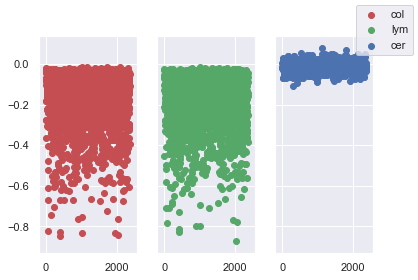
\includegraphics[width=15cm]{obipy-resources/test_water_chitin.png}
\caption{\label{test_water_chitin.png}
Are there differences in chitin to water treatment? Here shows the Water - Chitin results, dots are genes, down low values are up-regulated, larger ones are down regulated, near 0 genes are neutrally inclined}
\end{figure}


\paragraph{Col exclusive genes for Col and Lym at 05hr W/C treatments}
\label{sec:org19d4a0c}
\begin{center}
\begin{tabular}{rlll}
 & incoming & name & description\\
\hline
0 & AT5G67570 & DG1 & Pentatricopeptide repeat-containing protein At5g67570, chloroplastic\\
1 & AT5G67430 & AT5G67430 & Acyl-CoA N-acyltransferases (NAT) superfamily protein\\
2 & AT5G67140 & AT5G67140 & F-box protein At5g67140\\
3 & AT5G66910 & AT5G66910 & Probable disease resistance protein At5g66910\\
4 & AT5G66558 & AT5G66558 & other RNA\\
5 & AT5G66060 & P4H10 & Probable prolyl 4-hydroxylase 10\\
6 & AT5G65870 & PSK5 & Phytosulfokines 5\\
7 & AT5G65660 & AT5G65660 & Uncharacterized protein At5g65660\\
8 & AT5G65590 & DOF5.7 & Dof zinc finger protein DOF5.7\\
9 & AT5G65210 & TGA1 & Transcription factor TGA1\\
10 & AT5G64850 & AT5G64850 & At5g64850\\
11 & AT5G64360 & AT5G64360 & AT5G64360 protein\\
12 & AT5G64060 & anac103 & NAC domain containing protein 103\\
13 & AT5G63770 & DGK2 & Diacylglycerol kinase 2\\
14 & AT5G61440 & ACHT5 & Thioredoxin-like 1-2, chloroplastic\\
15 & AT5G61340 & AT5G61340 & Transmembrane protein\\
16 & AT5G60890 & MYB34 & Transcription factor MYB34\\
17 & AT5G60050 & AT5G60050 & BTB/POZ domain-containing protein At5g60050\\
18 & AT5G59990 & AT5G59990 & CCT motif family protein\\
19 & AT5G59950 & AT5G59950 & RNA-binding (RRM/RBD/RNP motifs) family protein\\
20 & AT5G59580 & UGT76E1 & UDP-glycosyltransferase 76E1\\
21 & AT5G57440 & GPP2 & (DL)-glycerol-3-phosphatase 2\\
22 & AT5G57230 & AT5G57230 & Thioredoxin superfamily protein\\
23 & AT5G56140 & AT5G56140 & KH domain-containing protein At5g56140\\
24 & AT5G54840 & SGP1 & Ras-related small GTP-binding family protein\\
25 & AT5G54650 & FH5 & Formin-like protein 5\\
26 & AT5G53590 & AT5G53590 & At5g53590\\
27 & AT5G53450 & PAP14 & Probable plastid-lipid-associated protein 14, chloroplastic\\
28 & AT5G52810 & SARD4 & Protein SAR DEFICIENT 4\\
29 & AT5G52800 & AT5G52800 & DNA primase\\
30 & AT5G52545 & AT5G52545 & unknown protein\\
31 & AT5G52180 & AT5G52180 & Dbj\\
32 & AT5G51670 & AT5G51670 & Similarity to unknown protein\\
33 & AT5G51400 & AT5G51400 & Gene1000 protein\\
34 & AT5G48250 & COL10 & Zinc finger protein CONSTANS-LIKE 10\\
35 & AT5G47370 & HAT2 & Homeobox-leucine zipper protein HAT2\\
36 & AT5G46160 & HLP & 50S ribosomal protein HLP, mitochondrial\\
37 & AT5G45320 & AT5G45320 & Late embryogenesis abundant protein\\
38 & AT5G44565 & AT5G44565 & unknown protein\\
39 & AT5G44180 & RLT2 & Homeobox-DDT domain protein RLT2\\
40 & AT5G44130 & FLA13 & Fasciclin-like arabinogalactan protein 13\\
41 & AT5G43630 & TZP & Zinc knuckle (CCHC-type) family protein\\
42 & AT5G43470 & RPP8 & Disease resistance protein RPP8\\
43 & AT5G42750 & BKI1 & BRI1 kinase inhibitor 1\\
44 & AT5G42130 & MFL1 & Protein MITOFERRINLIKE 1, chloroplastic\\
45 & AT5G39990 & GLCAT14A & Beta-glucuronosyltransferase GlcAT14A\\
46 & AT5G38350 & AT5G38350 & Disease resistance protein (NBS-LRR class) family\\
47 & AT5G38310 & AT5G38310 & Putative uncharacterized protein\\
48 & AT5G35753 & AT5G35753 & Domain of unknown function (DUF3444)\\
49 & AT5G27520 & PNC2 & PNC2\\
50 & AT5G25840 & AT5G25840 & DUF1677 family protein (DUF1677)\\
51 & AT5G25620 & YUC6 & Flavin-binding monooxygenase family protein\\
52 & AT5G25240 & AT5G25240 & Stress induced protein\\
53 & AT5G25180 & CYP71B14 & Cytochrome P450 71B14\\
54 & AT5G25060 & RRC1 & Protein RRC1\\
55 & AT5G24570 & AT5G24570 & Putative uncharacterized protein\\
56 & AT5G24400 & PGL3 & Probable 6-phosphogluconolactonase 5, chloroplastic\\
57 & AT5G24010 & AT5G24010 & Probable receptor-like protein kinase At5g24010\\
58 & AT5G23860 & TUBB8 & Tubulin beta chain\\
59 & AT5G23680 & AT5G23680 & At5g23680\\
60 & AT5G21960 & ERF016 & Ethylene-responsive transcription factor ERF016\\
61 & AT5G20840 & SAC4 & Phosphoinositide phosphatase SAC4\\
62 & AT5G20620 & UBQ4 & Polyubiquitin 4\\
63 & AT5G18475 & AT5G18475 & Pentatricopeptide repeat-containing protein At5g18475\\
64 & AT5G18460 & AT5G18460 & At5g18460\\
65 & AT5G18430 & AT5G18430 & GDSL esterase/lipase At5g18430\\
66 & AT5G18255 & AT5G18255 & other RNA\\
67 & AT5G17780 & AT5G17780 & alpha/beta-Hydrolases superfamily protein\\
68 & AT5G16200 & AT5G16200 & 50S ribosomal protein-like protein\\
69 & AT5G15770 & GNA1 & Glucosamine 6-phosphate N-acetyltransferase\\
70 & AT5G15740 & OFUT34 & O-fucosyltransferase 34\\
71 & AT5G15410 & CNGC2 & Cyclic nucleotide-gated ion channel 2\\
72 & AT5G15270 & AT5G15270 & RNA-binding KH domain-containing protein\\
73 & AT5G14350 & AT5G14350 & Pentatricopeptide repeat (PPR) superfamily protein\\
74 & AT5G13930 & CHS & Chalcone synthase family protein\\
75 & AT5G13780 & NAA10 & N-terminal acetyltransferase A complex catalytic subunit NAA10\\
76 & AT5G12050 & AT5G12050 & Protein BIG GRAIN 1-like D\\
77 & AT5G10965 & AT5G10965 & None\\
78 & AT5G09330 & NAC082 & NAC domain-containing protein 82\\
79 & AT5G08710 & AT5G08710 & RUG1\\
80 & AT5G08570 & AT5G08570 & Pyruvate kinase\\
81 & AT5G08135 & AT5G08135 & None\\
82 & AT5G07590 & AT5G07590 & At5g07590\\
83 & AT5G06835 & AT5G06835 & None\\
84 & AT5G06000 & EIF3G2 & Eukaryotic translation initiation factor 3 subunit G\\
85 & AT5G04820 & OFP13 & Transcription repressor OFP13\\
86 & AT5G03670 & AT5G03670 & TRM28\\
87 & AT5G03635 & AT5G03635 & None\\
88 & AT5G03330 & AT5G03330 & At5g03330\\
89 & AT5G03240 & UBQ3 & Ubiquitin 4\\
90 & AT5G02770 & MOS11 & Protein MODIFIER OF SNC1 11\\
91 & AT5G02480 & AT5G02480 & AT5g02480/T22P11\_70\\
92 & AT5G01990 & PILS6 & Protein PIN-LIKES 6\\
93 & AT5G01630 & BRCA2B & Protein BREAST CANCER SUSCEPTIBILITY 2 homolog B\\
94 & AT5G00965 & AT5G00965 & None\\
95 & AT4G39900 & AT4G39900 & AT4g39900/T5J17\_70\\
96 & AT4G39366 & AT4G39366 & snoRNA\\
97 & AT4G39361 & AT4G39361 & snoRNA\\
98 & AT4G37608 & AT4G37608 & Uncharacterized protein AT4g37600\\
99 & AT4G36920 & AP2 & Floral homeotic protein APETALA 2\\
100 & AT4G36810 & GGPPS1 & Heterodimeric geranylgeranyl pyrophosphate synthase large subunit 1, chloroplastic\\
101 & AT4G36808 & AT4G36808 & Potential natural antisense gene, locus overlaps with AT4G36810\\
102 & AT4G36240 & GATA7 & GATA transcription factor 7\\
103 & AT4G35730 & AT4G35730 & Regulator of Vps4 activity in the MVB pathway protein\\
104 & AT4G35470 & PIRL4 & Plant intracellular Ras-group-related LRR protein 4\\
105 & AT4G35320 & AT4G35320 & AT4g35320/F23E12\_120\\
106 & AT4G34920 & AT4G34920 & AT4g34920/F11I11\_160\\
107 & AT4G34810 & AT4G34810 & SAUR-like auxin-responsive protein family\\
108 & AT4G34800 & AT4G34800 & SAUR-like auxin-responsive protein family\\
109 & AT4G33470 & HDA14 & Histone deacetylase\\
110 & AT4G32440 & AT4G32440 & Plant Tudor-like RNA-binding protein\\
111 & AT4G32430 & PCMP-E40 & Pentatricopeptide repeat-containing protein At4g32430, mitochondrial\\
112 & AT4G31805 & POLAR & Protein POLAR LOCALIZATION DURING ASYMMETRIC DIVISION AND REDISTRIBUTION\\
113 & AT4G30790 & ATG11 & Autophagy-related protein 11\\
114 & AT4G30097 & AT4G30097 & unknown protein\\
115 & AT4G29240 & AT4G29240 & Extensin-like protein\\
116 & AT4G28680 & TYRDC & L-tyrosine decarboxylase\\
117 & AT4G27657 & AT4G27657 & At4g27657\\
118 & AT4G27654 & AT4G27654 & At4g27654\\
119 & AT4G27595 & AT4G27595 & Plant protein of unknown function (DUF827)\\
120 & AT4G27370 & VIIIB & P-loop containing nucleoside triphosphate hydrolases superfamily protein\\
121 & AT4G26610 & D6PKL1 & Serine/threonine-protein kinase D6PKL1\\
122 & AT4G26270 & PFK3 & ATP-dependent 6-phosphofructokinase 3\\
123 & AT4G26070 & MKK1 & NMAPKK\\
124 & AT4G25990 & CIL & CCT motif family protein (Fragment)\\
125 & AT4G25780 & AT4G25780 & CAP (Cysteine-rich secretory proteins, Antigen 5, and Pathogenesis-related 1 protein) superfamily protein\\
126 & AT4G25360 & TBL18 & TBL18\\
127 & AT4G24510 & CER2 & VC2\\
128 & AT4G24210 & GID2 & SLY1\\
129 & AT4G23230 & CRK15 & Cysteine-rich receptor-like protein kinase 15\\
130 & AT4G22790 & DTX56 & Protein DETOXIFICATION\\
131 & AT4G22530 & AT4G22530 & S-adenosyl-L-methionine-dependent methyltransferases superfamily protein\\
132 & AT4G21890 & AT4G21890 & At4g21890\\
133 & AT4G21510 & SKIP27 & F-box protein SKIP27\\
134 & AT4G19380 & AT4G19380 & Long-chain fatty alcohol dehydrogenase family protein\\
135 & AT4G19003 & VPS25 & Vacuolar protein sorting-associated protein 25\\
136 & AT4G18422 & AT4G18422 & unknown protein\\
137 & AT4G17660 & PBL20 & Probable serine/threonine-protein kinase PBL20\\
138 & AT4G15236 & ABCG43 & ABC-2 and Plant PDR ABC-type transporter family protein\\
139 & AT4G14990 & PAT1H2 & Protein PAT1 homolog 2\\
140 & AT4G14860 & OFP11 & Transcription repressor OFP11\\
141 & AT4G14050 & PCMP-H13 & Pentatricopeptide repeat-containing protein At4g14050, mitochondrial\\
142 & AT4G13820 & AT4G13820 & Disease resistance like protein\\
143 & AT4G12290 & AT4G12290 & Amine oxidase\\
144 & AT4G12010 & DSC1 & Disease resistance-like protein DSC1\\
145 & AT4G11640 & SR & Serine racemase\\
146 & AT4G11050 & AtGH9C3 & Endoglucanase 19\\
147 & AT4G09040 & AT4G09040 & At4g09040\\
148 & AT4G06598 & AT4G06598 & Uncharacterized protein At4g06598\\
149 & AT4G05910 & AT4G05910 & None\\
150 & AT4G04920 & MED16 & Mediator of RNA polymerase II transcription subunit 16\\
151 & AT4G04745 & AT4G04745 & At4g04745\\
152 & AT4G04670 & AT4G04670 & tRNA wybutosine-synthesizing protein 2/3/4\\
153 & AT4G03400 & DFL2 & Indole-3-acetic acid-amido synthetase GH3.10\\
154 & AT4G02630 & AT4G02630 & Protein kinase superfamily protein\\
155 & AT4G02440 & EID1 & Phytochrome A-associated F-box protein\\
156 & AT4G01900 & GLB1 & Nitrogen regulatory protein P-II homolog\\
157 & AT4G01037 & WTF1 & WTF1\\
158 & AT4G00730 & ANL2 & Homeobox-leucine zipper protein ANTHOCYANINLESS 2\\
159 & AT4G00030 & PAP11 & Probable plastid-lipid-associated protein 11, chloroplastic\\
160 & AT3G63255 & AT3G63255 & None\\
161 & AT3G63060 & EDL3 & EID1-like F-box protein 3\\
162 & AT3G61670 & AT3G61670 & Extra-large G-like protein, putative (DUF3133)\\
163 & AT3G61090 & AT3G61090 & At3g61090\\
164 & AT3G60550 & CYCU2-2 & Cyclin-U2-2\\
165 & AT3G60250 & CKB3 & Casein kinase II subunit beta-3\\
166 & AT3G60220 & ATL4 & TL4\\
167 & AT3G59980 & AT3G59980 & Nucleic acid-binding, OB-fold-like protein\\
168 & AT3G59810 & LSM6A & Sm-like protein LSM6A\\
169 & AT3G57540 & REM4.1 & Remorin 4.1\\
170 & AT3G56260 & AT3G56260 & At3g56260\\
171 & AT3G56110 & PRA1B1 & PRA1 family protein\\
172 & AT3G55360 & ECR & TSC13\\
173 & AT3G55120 & CHI1 & Chalcone--flavonone isomerase 1\\
174 & AT3G54950 & PLP7 & Patatin-like protein 7\\
175 & AT3G52470 & AT3G52470 & Late embryogenesis abundant (LEA) hydroxyproline-rich glycoprotein family\\
176 & AT3G51980 & AT3G51980 & ARM repeat superfamily protein\\
177 & AT3G49690 & RAX3 & RAX3\\
178 & AT3G48850 & MPT2 & Mitochondrial phosphate carrier protein 2, mitochondrial\\
179 & AT3G48800 & AT3G48800 & Sterile alpha motif (SAM) domain-containing protein\\
180 & AT3G47680 & AT3G47680 & At3g47680\\
181 & AT3G46590 & TRP2 & Telomere repeat-binding protein 2\\
182 & AT3G46080 & ZAT8 & Zinc finger protein ZAT8\\
183 & AT3G45830 & AT3G45830 & DNA-binding protein-like\\
184 & AT3G29639 & AT3G29639 & BEST Arabidopsis thaliana protein match is: SPOC domain / Transcription elongation factor S-II protein (TAIR:AT5G11430.1)\\
185 & AT3G28690 & AT3G28690 & Protein kinase superfamily protein\\
186 & AT3G27540 & AT3G27540 & Beta-1,4-N-acetylglucosaminyltransferase family protein\\
187 & AT3G27060 & TSO2 & TSO2\\
188 & AT3G26190 & CYP71B21 & Cytochrome P450 71B21\\
189 & AT3G25882 & NIMIN-2 & NIMIN-2\\
190 & AT3G25640 & AT3G25640 & Protein of unknown function, DUF617\\
191 & AT3G21230 & 4CL4 & 4-coumarate--CoA ligase 4\\
192 & AT3G21140 & AT3G21140 & Pyridoxamine 5'-phosphate oxidase family protein\\
193 & AT3G20898 & SMR13 & Cyclin-dependent protein kinase inhibitor SMR13\\
194 & AT3G18070 & BGLU43 & Beta-glucosidase 43\\
195 & AT3G17920 & AT3G17920 & Outer arm dynein light chain 1 protein\\
196 & AT3G17120 & AT3G17120 & AT3g17120/K14A17\_24\\
197 & AT3G17040 & HCF107 & Protein high chlorophyll fluorescent 107\\
198 & AT3G15700 & AT3G15700 & P-loop containing nucleoside triphosphate hydrolases superfamily protein\\
199 & AT3G15030 & TCP4 & TCP4\\
200 & AT3G14810 & MSL5 & Mechanosensitive ion channel protein 5\\
201 & AT3G13950 & AT3G13950 & AT3G13950 protein\\
202 & AT3G13520 & AGP12 & Arabinogalactan protein 12\\
203 & AT3G07870 & AT3G07870 & F-box protein At3g07870\\
204 & AT3G07730 & AT3G07730 & F17A17.7 protein\\
205 & AT3G06890 & AT3G06890 & At3g06890\\
206 & AT3G06780 & AT3G06780 & F3E22.8 protein\\
207 & AT3G06778 & AT3G06778 & Chaperone DnaJ-domain superfamily protein\\
208 & AT3G06570 & AT3G06570 & F-box/kelch-repeat protein At3g06570\\
209 & AT3G05675 & AT3G05675 & BTB/POZ domain-containing protein\\
210 & AT3G05650 & AtRLP32 & Receptor-like protein 32\\
211 & AT3G05350 & APP2 & Aminopeptidase P2\\
212 & AT3G04810 & NEK2 & Serine/threonine-protein kinase Nek2\\
213 & AT3G04580 & EIN4 & Ethylene receptor\\
214 & AT3G04070 & NAC047 & NAC transcription factor 47\\
215 & AT3G01895 & AT3G01895 & None\\
216 & AT3G01860 & AT3G01860 & Uncharacterized protein At3g01860\\
217 & AT3G01360 & AT3G01360 & At3g01360\\
218 & AT3G01320 & SNL1 & Paired amphipathic helix protein Sin3-like 1\\
219 & AT2G48080 & AT2G48080 & Oxidoreductase, 2OG-Fe(II) oxygenase family protein\\
220 & AT2G46660 & CYP78A6 & Cytochrome P450 78A6\\
221 & AT2G45970 & CYP86A8 & Cytochrome P450 86A8\\
222 & AT2G44760 & AT2G44760 & Domain of unknown function (DUF3598)\\
223 & AT2G44730 & AT2G44730 & Alcohol dehydrogenase transcription factor Myb/SANT-like family protein\\
224 & AT2G44700 & AT2G44700 & F-box/kelch-repeat protein At2g44700\\
225 & AT2G44070 & AT2G44070 & NagB/RpiA/CoA transferase-like superfamily protein\\
226 & AT2G42760 & AT2G42760 & At2g42760\\
227 & AT2G42580 & TTL3 & Inactive TPR repeat-containing thioredoxin TTL3\\
228 & AT2G42290 & AT2G42290 & Leucine-rich repeat protein kinase family protein\\
229 & AT2G42190 & AT2G42190 & Expressed protein\\
230 & AT2G41800 & AT2G41800 & At2g41800/T11A7.10\\
231 & AT2G41342 & AT2G41342 & Putative uncharacterized protein\\
232 & AT2G41231 & AT2G41231 & unknown protein.\\
233 & AT2G40690 & GLY1 & Glycerol-3-phosphate dehydrogenase\\
234 & AT2G40230 & AT2G40230 & HXXXD-type acyl-transferase family protein\\
235 & AT2G40150 & TBL28 & Protein trichome birefringence-like 28\\
236 & AT2G39950 & AT2G39950 & At2g39950\\
237 & AT2G39710 & AT2G39710 & Eukaryotic aspartyl protease family protein\\
238 & AT2G38820 & AT2G38820 & Protein of unknown function (DUF506)\\
239 & AT2G38390 & PER23 & Peroxidase 23\\
240 & AT2G37910 & AT2G37910 & At2g37910\\
241 & AT2G37810 & AT2G37810 & Cysteine/Histidine-rich C1 domain family protein\\
242 & AT2G37750 & AT2G37750 & Expressed protein\\
243 & AT2G37650 & SCL9 & Scarecrow-like protein 9\\
244 & AT2G37035 & AT2G37035 & unknown protein\\
245 & AT2G37020 & AT2G37020 & Translin family protein\\
246 & AT2G36790 & UGT73C6 & Glycosyltransferase (Fragment)\\
247 & AT2G36540 & AT2G36540 & Haloacid dehalogenase-like hydrolase (HAD) superfamily protein\\
248 & AT2G36050 & OFP15 & OFP15\\
249 & AT2G35660 & CTF2A & FAD/NAD(P)-binding oxidoreductase family protein\\
250 & AT2G35650 & CSLA7 & Glucomannan 4-beta-mannosyltransferase 7\\
251 & AT2G34830 & WRKY35 & WRKY DNA-binding protein 35\\
252 & AT2G34570 & MEE21 & PIN domain-like family protein\\
253 & AT2G34250 & AT2G34250 & AT2G34250 protein\\
254 & AT2G34010 & SPEAR2 & Protein SPEAR2\\
255 & AT2G33480 & NAC041 & NAC domain-containing protein 41\\
256 & AT2G32710 & KRP4 & Cyclin-dependent kinase inhibitor 4\\
257 & AT2G31200 & ADF6 & Actin-depolymerizing factor 6\\
258 & AT2G30620 & AT2G30620 & Histone H1.2\\
259 & AT2G30010 & TBL45 & TRICHOME BIREFRINGENCE-LIKE 45\\
260 & AT2G29900 & PS2 & Presenilin-like protein At2g29900\\
261 & AT2G29060 & SCL33 & Scarecrow-like protein 33\\
262 & AT2G28740 & HIS4 & Histone H4\\
263 & AT2G28650 & ATEXO70H8 & Exocyst subunit Exo70 family protein\\
264 & AT2G28510 & DOF2.1 & Dof zinc finger protein DOF2.1\\
265 & AT2G27210 & BSL3 & Serine/threonine-protein phosphatase BSL3\\
266 & AT2G26640 & KCS11 & 3-ketoacyl-CoA synthase 11\\
267 & AT2G26600 & AT2G26600 & Glycosyl hydrolase superfamily protein\\
268 & AT2G26280 & CID7 & Polyadenylate-binding protein-interacting protein 7\\
269 & AT2G25590 & AT2G25590 & Plant Tudor-like protein\\
270 & AT2G24320 & AT2G24320 & alpha/beta-Hydrolases superfamily protein\\
271 & AT2G23755 & AT2G23755 & Transmembrane family 220 helix protein\\
272 & AT2G23150 & NRAMP3 & Metal transporter Nramp3\\
273 & AT2G22800 & HAT9 & HAT9\\
274 & AT2G22490 & CYCD2;1 & Cyclin D21\\
275 & AT2G22010 & RKP & Related to KPC1\\
276 & AT2G21180 & AT2G21180 & At2g21180/F26H11.6\\
277 & AT2G20340 & ELI5 & Tyrosine decarboxylase 1\\
278 & AT2G18300 & AT2G18300 & Basic helix-loop-helix (BHLH) DNA-binding superfamily protein\\
279 & AT2G18193 & AT2G18193 & AAA-ATPase At2g18193\\
280 & AT2G17265 & HSK & Homoserine kinase\\
281 & AT2G17050 & AT2G17050 & disease resistance protein (TIR-NBS-LRR class), putative\\
282 & AT2G16890 & UGT90A1 & UDP-glycosyltransferase 90A1\\
283 & AT2G16720 & MYB7 & Transcription factor MYB7\\
284 & AT2G14290 & AT2G14290 & F-box protein At2g14290\\
285 & AT2G09370 & AT2G09370 & None\\
286 & AT2G08730 & AT2G08730 & None\\
287 & AT2G04965 & AT2G04965 & None\\
288 & AT2G04560 & LPXB & Probable lipid-A-disaccharide synthase, mitochondrial\\
289 & AT2G03830 & RGF8 & Probable root meristem growth factor 8\\
290 & AT2G03810 & AT2G03810 & 18S pre-ribosomal assembly protein gar2-like protein\\
291 & AT2G02930 & GSTF3 & Glutathione S-transferase F3\\
292 & AT2G02680 & AT2G02680 & Cysteine/Histidine-rich C1 domain family protein\\
293 & AT1G79570 & AT1G79570 & Kinase superfamily with octicosapeptide/Phox/Bem1p domain-containing protein\\
294 & AT1G79160 & AT1G79160 & Filamentous hemagglutinin transporter\\
295 & AT1G78600 & LZF1 & Light-regulated zinc finger protein 1\\
296 & AT1G78265 & AT1G78265 & other RNA\\
297 & AT1G77850 & ARF17 & auxin response factor 17\\
298 & AT1G77250 & AT1G77250 & At1g77250\\
299 & AT1G76952 & IDL5 & inflorescence deficient in abscission (IDA)-like 5\\
300 & AT1G76810 & AT1G76810 & Eukaryotic translation initiation factor 2 (eIF-2) family protein\\
301 & AT1G76040 & CPK29 & calcium-dependent protein kinase 29\\
302 & AT1G75860 & AT1G75860 & unknown protein\\
303 & AT1G75770 & AT1G75770 & At1g75770/F10A5\_10\\
304 & AT1G75730 & AT1G75730 & At1g75730\\
305 & AT1G75590 & AT1G75590 & SAUR-like auxin-responsive protein family\\
306 & AT1G73010 & PS2 & Inorganic pyrophosphatase 1\\
307 & AT1G72640 & AT1G72640 & At1g72640\\
308 & AT1G72510 & AT1G72510 & At1g72510\\
309 & AT1G72360 & HRE1 & Integrase-type DNA-binding superfamily protein\\
310 & AT1G72340 & AT1G72340 & NagB/RpiA/CoA transferase-like superfamily protein\\
311 & AT1G71866 & EPFL7 & EPIDERMAL PATTERNING FACTOR-like protein 7\\
312 & AT1G71190 & SAG18 & At1g71190\\
313 & AT1G71030 & ATMYBL2 & At1g71030/F23N20\_2\\
314 & AT1G70610 & ABCB26 & ABC transporter B family member 26, chloroplastic\\
315 & AT1G69790 & PBL18 & Probable serine/threonine-protein kinase PBL18\\
316 & AT1G68880 & BZIP8 & Basic leucine zipper 8\\
317 & AT1G66465 & AT1G66465 & Transmembrane protein\\
318 & AT1G65380 & CLV2 & Receptor-like protein CLAVATA2\\
319 & AT1G65240 & AT1G65240 & Aspartic proteinase-like protein 2\\
320 & AT1G64530 & NLP6 & Protein NLP6\\
321 & AT1G63700 & YDA & YDA\\
322 & AT1G62950 & AT1G62950 & F16P17.10 protein\\
323 & AT1G62520 & AT1G62520 & Sulfated surface-like glycoprotein\\
324 & AT1G62305 & AT1G62305 & At1g62305\\
325 & AT1G61860 & AT1G61860 & Protein kinase superfamily protein\\
326 & AT1G61840 & AT1G61840 & Cysteine/Histidine-rich C1 domain family protein\\
327 & AT1G61610 & AT1G61610 & Serine/threonine-protein kinase\\
328 & AT1G61410 & AT1G61410 & At1g61410\\
329 & AT1G60270 & BGLU6 & Putative beta-glucosidase 6\\
330 & AT1G60000 & AT1G60000 & AT1G60000 protein\\
331 & AT1G59950 & AT1G59950 & Aldo/keto reductase\\
332 & AT1G58400 & AT1G58400 & Putative disease resistance protein At1g58400\\
333 & AT1G56430 & NAS4 & Probable nicotianamine synthase 4\\
334 & AT1G56260 & TEN1 & CST complex subunit TEN1\\
335 & AT1G56020 & AT1G56020 & At1g56020\\
336 & AT1G55390 & AT1G55390 & Cysteine/Histidine-rich C1 domain family protein\\
337 & AT1G54650 & AT1G54650 & Methyltransferase family protein\\
338 & AT1G52880 & NAC018 & NARS2\\
339 & AT1G52550 & AT1G52550 & At1g52550\\
340 & AT1G51780 & ILL5 & IAA-amino acid hydrolase ILR1-like 5\\
341 & AT1G51170 & UNC & Serine/threonine-protein kinase UCN\\
342 & AT1G50510 & AT1G50510 & Indigoidine synthase A family protein\\
343 & AT1G50180 & AT1G50180 & Putative disease resistance protein At1g50180\\
344 & AT1G50000 & AT1G50000 & Methyltransferase\\
345 & AT1G49840 & AT1G49840 & Glutamyl-tRNA (Gln) amidotransferase subunit A (DUF620)\\
346 & AT1G49510 & emb1273 & At1g49510\\
347 & AT1G48460 & AT1G48460 & At1g48460\\
348 & AT1G48300 & AT1G48300 & unknown protein\\
349 & AT1G45163 & AT1G45163 & unknown protein\\
350 & AT1G44120 & AT1G44120 & Armadillo/beta-catenin-like repeat\\
351 & AT1G35330 & AT1G35330 & RING/U-box superfamily protein\\
352 & AT1G31950 & AT1G31950 & Terpenoid cyclases/Protein prenyltransferases superfamily protein\\
353 & AT1G29720 & RFK1 & Probable LRR receptor-like serine/threonine-protein kinase At1g29720\\
354 & AT1G29357 & AT1G29357 & other RNA\\
355 & AT1G28310 & AT1G28310 & Dof-type zinc finger DNA-binding family protein\\
356 & AT1G28090 & AT1G28090 & Polynucleotide adenylyltransferase family protein\\
357 & AT1G27200 & AT1G27200 & DUF23/GT0 (Fragment)\\
358 & AT1G26730 & PHO1-H7 & Phosphate transporter PHO1 homolog 7\\
359 & AT1G26600 & CLE9 & CLAVATA3/ESR-RELATED 9\\
360 & AT1G26410 & FOX4 & Berberine bridge enzyme-like 6\\
361 & AT1G26208 & AT1G26208 & other RNA\\
362 & AT1G26130 & AT1G26130 & Phospholipid-transporting ATPase\\
363 & AT1G25450 & KCS5 & 3-ketoacyl-CoA synthase 5\\
364 & AT1G24530 & AT1G24530 & F21J9.19\\
365 & AT1G24350 & AT1G24350 & Acid phosphatase/vanadium-dependent haloperoxidase-related protein\\
366 & AT1G23052 & AT1G23052 & None\\
367 & AT1G22640 & MYB3 & MYB3\\
368 & AT1G22270 & TRM112A & Multifunctional methyltransferase subunit TRM112 homolog A\\
369 & AT1G22030 & AT1G22030 & BPS1-like protein\\
370 & AT1G21920 & AT1G21920 & Histone H3 K4-specific methyltransferase SET7/9 family protein\\
371 & AT1G21060 & AT1G21060 & Protein of unknown function, DUF547\\
372 & AT1G21000 & AT1G21000 & At1g21000/F9H16\_1\\
373 & AT1G19630 & CYP722A1 & Cytochrome P450, family 722, subfamily A, polypeptide 1\\
374 & AT1G19620 & AT1G19620 & unknown protein\\
375 & AT1G19170 & AT1G19170 & Pectin lyase-like superfamily protein\\
376 & AT1G17840 & ABCG11 & ABC transporter G family member 11\\
377 & AT1G16930 & AT1G16930 & F-box/FBD/LRR-repeat protein At1g16930\\
378 & AT1G16490 & MYB58 & Transcription factor MYB58\\
379 & AT1G16390 & OCT3 & Organic cation/carnitine transporter 3\\
380 & AT1G16260 & WAKL8 & Wall-associated receptor kinase-like 8\\
381 & AT1G16240 & SYP51 & SYP51\\
382 & AT1G16160 & WAKL5 & WAKL5\\
383 & AT1G15100 & RHA2A & E3 ubiquitin-protein ligase RHA2A\\
384 & AT1G14270 & AT1G14270 & CAAX amino terminal protease family protein\\
385 & AT1G13690 & ATE1 & ATE1\\
386 & AT1G13550 & AT1G13550 & Putative uncharacterized protein\\
387 & AT1G13250 & GATL3 & Probable galacturonosyltransferase-like 3\\
388 & AT1G13245 & RTFL17 & At1g13245\\
389 & AT1G13000 & AT1G13000 & Transmembrane protein, putative (DUF707)\\
390 & AT1G12460 & AT1G12460 & Probable LRR receptor-like serine/threonine-protein kinase At1g12460\\
391 & AT1G12200 & AT1G12200 & Flavin-containing monooxygenase\\
392 & AT1G11800 & AT1G11800 & At1g11800/F25C20\_3\\
393 & AT1G10550 & XTH33 & Probable xyloglucan endotransglucosylase/hydrolase protein 33\\
394 & AT1G10300 & AT1G10300 & Nucleolar GTP-binding protein 1\\
395 & AT1G10120 & BHLH74 & Transcription factor bHLH74\\
396 & AT1G09900 & AT1G09900 & Pentatricopeptide repeat-containing protein At1g09900\\
397 & AT1G09830 & PUR2 & Phosphoribosylamine--glycine ligase, chloroplastic\\
398 & AT1G09630 & RABA2A & Ras-related protein RABA2a\\
399 & AT1G08590 & PXL1 & Leucine-rich repeat receptor-like protein kinase PXL1\\
400 & AT1G08570 & ACHT4 & Thioredoxin-like 1-1, chloroplastic\\
401 & AT1G07900 & LBD1 & LBD1\\
402 & AT1G07753 & AT1G07753 & None\\
403 & AT1G07670 & ECA4 & Calcium-transporting ATPase 4, endoplasmic reticulum-type\\
404 & AT1G07530 & SCL14 & AT1G07530 protein\\
405 & AT1G07400 & HSP17.8 & 17.8 kDa class I heat shock protein\\
406 & AT1G07300 & AT1G07300 & josephin protein-related\\
407 & AT1G07150 & MAPKKK13 & F10K1.14 protein\\
408 & AT1G07090 & LSH6 & LSH6\\
409 & AT1G06980 & AT1G06980 & 6,7-dimethyl-8-ribityllumazine synthase\\
410 & AT1G05150 & AT1G05150 & Uncharacterized TPR repeat-containing protein At1g05150\\
411 & AT1G04767 & AT1G04767 & None\\
412 & AT1G04030 & AT1G04030 & unknown protein\\
413 & AT1G01610 & GPAT4 & GPAT4\\
\end{tabular}
\end{center}


\paragraph{Lym exclusive genes for Col and Lym at 05hr W/C treatment}
\label{sec:org3f7537a}
\begin{center}
\begin{tabular}{rlll}
 & incoming & name & description\\
\hline
0 & AT5G67440 & NPY3 & BTB/POZ domain-containing protein NPY3\\
1 & AT5G67400 & PER73 & Peroxidase\\
2 & AT5G67200 & AT5G67200 & Probable inactive receptor kinase At5g67200\\
3 & AT5G67190 & ERF010 & Ethylene-responsive transcription factor ERF010\\
4 & AT5G67150 & AT5G67150 & Anthranilate N-hydroxycinnamoyl/benzoyltransferase-like protein\\
5 & AT5G67070 & RALFL34 & Protein RALF-like 34\\
6 & AT5G66800 & AT5G66800 & Emb\\
7 & AT5G66631 & AT5G66631 & Pentatricopeptide repeat-containing protein At5g66631\\
8 & AT5G66490 & AT5G66490 & Uncharacterized protein At5g66490/K1F13\_15\\
9 & AT5G66200 & ARO2 & Armadillo repeat only 2\\
10 & AT5G66040 & STR16 & Thiosulfate sulfurtransferase 16, chloroplastic\\
11 & AT5G65690 & PCK2 & phosphoenolpyruvate carboxykinase 2\\
12 & AT5G65650 & AT5G65650 & Sugar transporter, putative (DUF1195)\\
13 & AT5G65613 & AT5G65613 & None\\
14 & AT5G65500 & AT5G65500 & U-box domain-containing protein kinase family protein\\
15 & AT5G65450 & UBP17 & ubiquitin-specific protease 17\\
16 & AT5G65410 & ZHD1 & Zinc-finger homeodomain protein 1\\
17 & AT5G65160 & TPR14 & At5g65160\\
18 & AT5G64670 & AT5G64670 & Ribosomal protein L18e/L15 superfamily protein\\
19 & AT5G64650 & AT5G64650 & At5g64650\\
20 & AT5G64500 & AT5G64500 & Probable sphingolipid transporter spinster homolog 2\\
21 & AT5G64470 & TBL12 & Protein trichome birefringence-like 12\\
22 & AT5G64450 & AT5G64450 & Emb\\
23 & AT5G64440 & FAAH & Fatty acid amide hydrolase\\
24 & AT5G64150 & AT5G64150 & At5g64156\\
25 & AT5G64130 & AT5G64130 & AT5G64130 protein\\
26 & AT5G63530 & HIPP07 & Heavy metal-associated isoprenylated plant protein 7\\
27 & AT5G63490 & CBSCBSPB1 & CBS domain-containing protein CBSCBSPB1\\
28 & AT5G63160 & BT1 & BTB/POZ and TAZ domain-containing protein 1\\
29 & AT5G63140 & PAP29 & Probable inactive purple acid phosphatase 29\\
30 & AT5G62940 & DOF5.6 & HCA2\\
31 & AT5G62865 & AT5G62865 & Uncharacterized protein At5g62860/MQB2\_160\\
32 & AT5G62720 & AT5G62720 & At5g62720\\
33 & AT5G62700 & TUBB3 & Tubulin beta-2 chain\\
34 & AT5G62690 & TUBB3 & Tubulin beta-2 chain\\
35 & AT5G62650 & AT5G62650 & AT5g62650/MRG21\_7\\
36 & AT5G62270 & AT5G62270 & Gb\\
37 & AT5G62190 & RH7 & DEAD-box ATP-dependent RNA helicase 7\\
38 & AT5G61830 & AT5G61830 & At5g61830\\
39 & AT5G61820 & AT5G61820 & Stress up-regulated Nod 19 protein\\
40 & AT5G61790 & CNX1 & Calnexin homolog 1\\
41 & AT5G61780 & TSN2 & Ribonuclease TUDOR 2\\
42 & AT5G61770 & PPAN & PETER PAN-like protein\\
43 & AT5G61530 & AT5G61530 & Uncharacterized Rho GTPase-activating protein At5g61530\\
44 & AT5G61480 & TDR & Leucine-rich repeat receptor-like protein kinase TDR\\
45 & AT5G61420 & MYB28 & PMG1\\
46 & AT5G61310 & AT5G61310 & Cytochrome c oxidase subunit 5C\\
47 & AT5G61260 & AT5G61260 & Emb\\
48 & AT5G61020 & ECT3 & ECT3\\
49 & AT5G61000 & RPA1D & Replication protein A subunit\\
50 & AT5G60990 & RH10 & DEAD-box ATP-dependent RNA helicase 10\\
51 & AT5G60960 & PNM1 & PNM1\\
52 & AT5G60800 & AT5G60800 & Heavy metal transport/detoxification superfamily protein\\
53 & AT5G60790 & ABCF1 & ABC transporter F family member 1\\
54 & AT5G60700 & AT5G60700 & Glycosyltransferase family protein 2\\
55 & AT5G60670 & RPL12C & 60S ribosomal protein L12-3\\
56 & AT5G60390 & A1 & Elongation factor 1-alpha 4\\
57 & AT5G60360 & AALP & Aleurain-like protease\\
58 & AT5G60280 & LECRK18 & L-type lectin-domain containing receptor kinase I.8\\
59 & AT5G60030 & AT5G60030 & Putative uncharacterized protein\\
60 & AT5G59850 & RPS15AF & 40S ribosomal protein S15a-1\\
61 & AT5G59540 & AT5G59540 & 1-aminocyclopropane-1-carboxylate oxidase homolog 12\\
62 & AT5G59030 & COPT1 & Copper transporter 1\\
63 & AT5G59020 & AT5G59020 & Gb\\
64 & AT5G58960 & GIL1 & Plant protein of unknown function (DUF641)\\
65 & AT5G58700 & PLC4 & Phosphoinositide phospholipase C 4\\
66 & AT5G58630 & AT5G58630 & TRM31\\
67 & AT5G58580 & ATL63 & RING-H2 finger protein ATL63\\
68 & AT5G58420 & RPS4D & 40S ribosomal protein S4-3\\
69 & AT5G58375 & AT5G58375 & At5g58375\\
70 & AT5G58320 & NET4A & Protein NETWORKED 4A\\
71 & AT5G58010 & BHLH82 & LRL3\\
72 & AT5G57910 & AT5G57910 & At5g57910\\
73 & AT5G57790 & AT5G57790 & unknown protein\\
74 & AT5G57685 & GDU3 & Protein GLUTAMINE DUMPER 3\\
75 & AT5G57655 & XYLA & Xylose isomerase\\
76 & AT5G57630 & CIPK21 & CBL-interacting serine/threonine-protein kinase 21\\
77 & AT5G57625 & AT5G57625 & At5g57625\\
78 & AT5G57550 & XTH25 & Probable xyloglucan endotransglucosylase/hydrolase protein 25\\
79 & AT5G57345 & AT5G57345 & At5g57345\\
80 & AT5G57290 & RPP3B & 60S acidic ribosomal protein P3-2\\
81 & AT5G57060 & AT5G57060 & 60S ribosomal L18a-like protein\\
82 & AT5G57020 & NMT1 & Glycylpeptide N-tetradecanoyltransferase 1\\
83 & AT5G56750 & NDL1 & Protein NDL1\\
84 & AT5G56530 & AT5G56530 & Similarity to carboxyl-terminal proteinase\\
85 & AT5G56030 & HSP81-2 & Heat shock protein 81-2\\
86 & AT5G56000 & HSP90-4 & Hsp81.4\\
87 & AT5G55920 & OLI2 & Nucleolar protein-like\\
88 & AT5G55790 & AT5G55790 & At5g55790\\
89 & AT5G55580 & MTERF9 & Transcription termination factor MTERF9, chloroplastic\\
90 & AT5G55120 & VTC5 & VTC5\\
91 & AT5G54930 & AT5G54930 & AT hook motif-containing protein\\
92 & AT5G54850 & AT5G54850 & At5g54850\\
93 & AT5G54780 & AT5G54780 & Ypt/Rab-GAP domain of gyp1p superfamily protein\\
94 & AT5G54640 & RAT5 & Histone H2A.6\\
95 & AT5G54510 & GH3.6 & GH3.6\\
96 & AT5G54300 & AT5G54300 & Cotton fiber expressed protein 1-like protein\\
97 & AT5G54180 & MTERF8 & PTAC15\\
98 & AT5G54130 & AT5G54130 & At5g54130\\
99 & AT5G54110 & PVA41 & Vesicle-associated protein 4-1\\
100 & AT5G53980 & ATHB-52 & Homeobox-leucine zipper protein ATHB-52\\
101 & AT5G53900 & AT5G53900 & Gb\\
102 & AT5G53830 & VQ33 & VQ motif-containing protein 33\\
103 & AT5G53420 & AT5G53420 & CCT motif family protein\\
104 & AT5G53300 & UBC10 & Ubiquitin-conjugating enzyme E2 10\\
105 & AT5G53180 & ATPTB2 & Polypyrimidine tract-binding protein homolog 2\\
106 & AT5G52920 & PKP2 & Pyruvate kinase\\
107 & AT5G52720 & AT5G52720 & Copper transport protein family\\
108 & AT5G52580 & AT5G52580 & RabGAP/TBC domain-containing protein\\
109 & AT5G52470 & MED36B & Probable mediator of RNA polymerase II transcription subunit 36b\\
110 & AT5G52410 & AT5G52410 & CONTAINS InterPro DOMAIN/s: S-layer homology domain (InterPro:IPR001119)\\
111 & AT5G52320 & CYP96A4 & CYP96A4\\
112 & AT5G52200 & I-2 & Protein phosphatase inhibitor 2\\
113 & AT5G52010 & AT5G52010 & AT5g52010/MSG15\_9\\
114 & AT5G51970 & SDH & Sorbitol dehydrogenase\\
115 & AT5G51850 & AT5G51850 & TRM24\\
116 & AT5G51690 & ACS12 & Probable aminotransferase ACS12\\
117 & AT5G51540 & OCT1 & Mitochondrial intermediate peptidase, mitochondrial\\
118 & AT5G50380 & ATEXO70F1 & Exocyst subunit Exo70 family protein\\
119 & AT5G50160 & FRO8 & Ferric reduction oxidase 8, mitochondrial\\
120 & AT5G49980 & AFB5 & AFB5\\
121 & AT5G49910 & HSP70-7 & Heat shock 70 kDa protein 7, chloroplastic\\
122 & AT5G49770 & AT5G49770 & Probable leucine-rich repeat receptor-like protein kinase At5g49770\\
123 & AT5G49660 & CEPR1 & Receptor protein-tyrosine kinase CEPR1\\
124 & AT5G49450 & BZIP1 & Basic leucine zipper 1\\
125 & AT5G49360 & BXL1 & Beta-D-xylosidase 1\\
126 & AT5G49280 & AT5G49280 & At5g49280\\
127 & AT5G48760 & RPL13AD & 60S ribosomal protein L13a-4\\
128 & AT5G48480 & AT5G48480 & Uncharacterized protein At5g48480\\
129 & AT5G48390 & ZIP4 & TPR repeat-containing protein ZIP4\\
130 & AT5G48160 & OBE2 & Protein OBERON 2\\
131 & AT5G47930 & RPS27D & 40S ribosomal protein S27-3\\
132 & AT5G47640 & NFYB2 & Nuclear transcription factor Y subunit B-2\\
133 & AT5G47320 & RPS19 & 40S ribosomal protein S19, mitochondrial\\
134 & AT5G47210 & RGGC & RGG repeats nuclear RNA binding protein C\\
135 & AT5G47200 & RABD2B & Ras-related protein RABD2b\\
136 & AT5G46250 & LARP6A & La-related protein 6A\\
137 & AT5G46170 & AT5G46170 & F-box protein At5g46170\\
138 & AT5G45800 & MEE62 & MEE62\\
139 & AT5G45775 & RPL11C & 60S ribosomal protein L11-2\\
140 & AT5G45430 & AT5G45430 & Protein kinase superfamily protein\\
141 & AT5G45420 & MAMYB & Transcription factor MAMYB\\
142 & AT5G45410 & AT5G45410 & AT5G45410 protein\\
143 & AT5G45260 & RRS1 & Disease resistance protein RRS1\\
144 & AT5G45080 & PP2A6 & Protein PHLOEM PROTEIN 2-LIKE A6\\
145 & AT5G45050 & RRS1B & Disease resistance protein RRS1B\\
146 & AT5G44930 & ARAD2 & Probable arabinosyltransferase ARAD2\\
147 & AT5G44610 & PCAP2 & Plasma membrane-associated cation-binding protein 2\\
148 & AT5G44572 & AT5G44572 & Transmembrane protein\\
149 & AT5G44480 & DUR & Putative UDP-arabinose 4-epimerase 4\\
150 & AT5G44380 & AT5G44380 & FAD-binding Berberine family protein\\
151 & AT5G44050 & DTX28 & Protein DETOXIFICATION 28\\
152 & AT5G43960 & AT5G43960 & Gb\\
153 & AT5G43790 & PCMP-E30 & Pentatricopeptide repeat-containing protein At5g43790\\
154 & AT5G43740 & AT5G43740 & Probable disease resistance protein At5g43740\\
155 & AT5G43210 & AT5G43210 & Emb\\
156 & AT5G43100 & AT5G43100 & Eukaryotic aspartyl protease family protein\\
157 & AT5G42870 & PAH2 & Phosphatidate phosphatase PAH2\\
158 & AT5G42770 & AT5G42770 & Maf-like protein\\
159 & AT5G42480 & ARC6 & Protein ACCUMULATION AND REPLICATION OF CHLOROPLASTS 6, chloroplastic\\
160 & AT5G42320 & AT5G42320 & Zn-dependent exopeptidases superfamily protein\\
161 & AT5G42300 & UBL5 & UBL5\\
162 & AT5G42140 & AT5G42140 & Regulator of chromosome condensation (RCC1) family with FYVE zinc finger domain\\
163 & AT5G42000 & AT5G42000 & At5g42000\\
164 & AT5G41990 & WNK8 & Serine/threonine-protein kinase WNK8\\
165 & AT5G41920 & SCL23 & Scarecrow-like protein 23\\
166 & AT5G41790 & CIP1 & COP1-interactive protein 1\\
167 & AT5G41730 & AT5G41730 & Protein kinase family protein\\
168 & AT5G41670 & PGD3 & 6-phosphogluconate dehydrogenase, decarboxylating\\
169 & AT5G41170 & AT5G41170 & Pentatricopeptide repeat-containing protein At5g41170, mitochondrial\\
170 & AT5G40690 & AT5G40690 & At5g40690\\
171 & AT5G40580 & PBB2 & Proteasome subunit beta type-7-B\\
172 & AT5G40450 & AT5G40450 & unknown protein\\
173 & AT5G39740 & RPL5B & RPL5B\\
174 & AT5G39590 & AT5G39590 & TLD-domain containing nucleolar protein\\
175 & AT5G39360 & EDL2 & EDL2\\
176 & AT5G39110 & AT5G39110 & Germin-like protein subfamily 1 member 14\\
177 & AT5G38940 & AT5G38940 & RmlC-like cupins superfamily protein\\
178 & AT5G38890 & AT5G38890 & AT5G38890 protein\\
179 & AT5G38360 & AT5G38360 & alpha/beta-Hydrolases superfamily protein\\
180 & AT5G38280 & PR5K & PR5-like receptor kinase\\
181 & AT5G38200 & AT5G38200 & Class I glutamine amidotransferase-like superfamily protein\\
182 & AT5G37740 & AT5G37740 & Calcium-dependent lipid-binding (CaLB domain) family protein\\
183 & AT5G37450 & AT5G37450 & Leucine-rich repeat protein kinase family protein\\
184 & AT5G37130 & AT5G37130 & Protein prenylyltransferase superfamily protein\\
185 & AT5G37070 & AT5G37070 & At5g37070\\
186 & AT5G36930 & AT5G36930 & Disease resistance protein (TIR-NBS-LRR class) family\\
187 & AT5G35840 & PHYC & Phytochrome C\\
188 & AT5G35732 & AT5G35732 & unknown protein\\
189 & AT5G35530 & RPS3C & 40S ribosomal protein S3-3\\
190 & AT5G35320 & AT5G35320 & DBH-like monooxygenase\\
191 & AT5G35190 & AT5G35190 & Proline-rich extensin-like family protein\\
192 & AT5G28919 & AT5G28919 & Putative uncharacterized protein\\
193 & AT5G28540 & MED37A & Mediator of RNA polymerase II transcription subunit 37a\\
194 & AT5G28300 & AT5G28300 & Trihelix transcription factor GTL2\\
195 & AT5G28060 & RPS24B & 40S ribosomal protein S24-2\\
196 & AT5G28050 & AT5G28050 & Cytidine/deoxycytidylate deaminase family protein\\
197 & AT5G27850 & RPL18C & 60S ribosomal protein L18-3\\
198 & AT5G27840 & TOPP8 & Calcineurin-like metallo-phosphoesterase superfamily protein\\
199 & AT5G27770 & RPL22C & 60S ribosomal protein L22-3\\
200 & AT5G27600 & LACS7 & Long chain acyl-CoA synthetase 7, peroxisomal\\
201 & AT5G27490 & AT5G27490 & Protein YIPF\\
202 & AT5G27330 & AT5G27330 & Prefoldin chaperone subunit family protein\\
203 & AT5G27120 & NOP5-1 & Probable nucleolar protein 5-1\\
204 & AT5G26910 & AT5G26910 & TRM8\\
205 & AT5G26751 & ASK1 & Shaggy-related protein kinase alpha\\
206 & AT5G26742 & RH3 & RH3\\
207 & AT5G26680 & AT5G26680 & Flap endonuclease 1\\
208 & AT5G26622 & AT5G26622 & Beta-galactosidase related protein\\
209 & AT5G26310 & UGT72E3 & Glycosyltransferase (Fragment)\\
210 & AT5G26180 & AT5G26180 & S-adenosyl-L-methionine-dependent methyltransferases superfamily protein\\
211 & AT5G25810 & TINY & Tny\\
212 & AT5G25630 & AT5G25630 & Tetratricopeptide repeat (TPR)-like superfamily protein\\
213 & AT5G25360 & AT5G25360 & unknown protein\\
214 & AT5G24840 & AT5G24840 & tRNA (guanine-N(7)-)-methyltransferase\\
215 & AT5G24830 & AT5G24830 & Pentatricopeptide repeat-containing protein At5g24830\\
216 & AT5G24670 & AT5G24670 & Cytidine/deoxycytidylate deaminase family protein\\
217 & AT5G24660 & LSU2 & Protein RESPONSE TO LOW SULFUR 2\\
218 & AT5G24600 & AT5G24600 & At5g24600\\
219 & AT5G24520 & TTG1 & Protein TRANSPARENT TESTA GLABRA 1\\
220 & AT5G24160 & SQE6 & Squalene epoxidase 6\\
221 & AT5G24100 & AT5G24100 & Inactive leucine-rich repeat receptor-like serine/threonine-protein kinase At5g24100\\
222 & AT5G23990 & ATFRO5 & ferric reduction oxidase 5\\
223 & AT5G23800 & ATDUF10 & DOMAIN OF UNKNOWN FUNCTION 724 10\\
224 & AT5G23740 & RPS11C & RPS11-BETA\\
225 & AT5G23480 & AT5G23480 & SWIB/MDM2 domain\\
226 & AT5G23250 & AT5G23250 & Succinate--CoA ligase\\
227 & AT5G22650 & HDT2 & Histone deacetylase HDT2\\
228 & AT5G22440 & RPL10AC & 60S ribosomal protein L10a-3\\
229 & AT5G22410 & PER60 & Peroxidase 60\\
230 & AT5G22380 & NAC090 & NAC-domain protein-like\\
231 & AT5G22290 & NAC089 & NAC domain-containing protein 89\\
232 & AT5G21940 & AT5G21940 & At5g21940\\
233 & AT5G20350 & PAT24 & Protein S-acyltransferase 24\\
234 & AT5G20290 & RPS8A & 40S ribosomal protein S8\\
235 & AT5G19860 & AT5G19860 & At5g19860\\
236 & AT5G19750 & AT5G19750 & Peroxisomal membrane 22 kDa (Mpv17/PMP22) family protein\\
237 & AT5G19510 & AT5G19510 & Elongation factor 1-beta 2\\
238 & AT5G19450 & CPK8 & Calcium-dependent protein kinase 8\\
239 & AT5G19210 & RH58 & DEAD-box ATP-dependent RNA helicase 58, chloroplastic\\
240 & AT5G19110 & AT5G19110 & Eukaryotic aspartyl protease family protein\\
241 & AT5G19090 & HIPP33 & Heavy metal-associated isoprenylated plant protein 33\\
242 & AT5G19080 & LUL3 & Probable E3 ubiquitin-protein ligase LUL3\\
243 & AT5G18690 & AGP25 & ATAGP25\\
244 & AT5G18260 & AT5G18260 & RING/U-box superfamily protein\\
245 & AT5G18220 & AT5G18220 & Beta-1,3-glucanase-like protein\\
246 & AT5G18065 & HTT3 & unknown protein\\
247 & AT5G17790 & VAR3 & Zinc finger protein VAR3, chloroplastic\\
248 & AT5G17600 & ATL52 & RING-H2 finger protein ATL52\\
249 & AT5G17240 & SDG40 & Protein SET DOMAIN GROUP 40\\
250 & AT5G16750 & TOZ & Transducin family protein / WD-40 repeat family protein\\
251 & AT5G16660 & AT5G16660 & Low-density receptor-like protein\\
252 & AT5G16320 & FRL1 & FRIGIDA-like protein 1\\
253 & AT5G16130 & RPS7C & 40S ribosomal protein S7-3\\
254 & AT5G16000 & NIK1 & Protein NSP-INTERACTING KINASE 1\\
255 & AT5G15930 & PAM1 & Plant adhesion molecule 1 (PAM1)\\
256 & AT5G15520 & RPS19B & 40S ribosomal protein S19-2\\
257 & AT5G15200 & RPS9B & 40S ribosomal protein S9-1\\
258 & AT5G14210 & AT5G14210 & Leucine-rich repeat protein kinase family protein\\
259 & AT5G14120 & AT5G14120 & Major facilitator superfamily protein\\
260 & AT5G14050 & AT5G14050 & U3 small nucleolar RNA-associated protein 18 homolog\\
261 & AT5G13950 & AT5G13950 & unknown protein\\
262 & AT5G13760 & AT5G13760 & Plasma-membrane choline transporter family protein\\
263 & AT5G13420 & AT5G13420 & Aldolase-type TIM barrel family protein\\
264 & AT5G13140 & AT5G13140 & Pollen Ole e 1 allergen and extensin family protein\\
265 & AT5G12410 & AT5G12410 & At5g12410/At5g12410\\
266 & AT5G12300 & AT5G12300 & At5g12300\\
267 & AT5G11790 & NDL2 & Protein NDL2\\
268 & AT5G11200 & AT5G11200 & DEAD/DEAH box RNA helicase family protein\\
269 & AT5G11170 & RH15 & DEAD-box ATP-dependent RNA helicase 56\\
270 & AT5G11060 & KNAT4 & KNAT4\\
271 & AT5G10580 & AT5G10580 & Protein of unknown function, DUF599\\
272 & AT5G10530 & LECRK91 & L-type lectin-domain containing receptor kinase IX.1\\
273 & AT5G10410 & AT5G10410 & Putative clathrin assembly protein At5g10410\\
274 & AT5G10360 & RPS6B & 40S ribosomal protein S6\\
275 & AT5G10350 & PABN3 & Polyadenylate-binding protein 3\\
276 & AT5G10210 & AT5G10210 & At5g10210\\
277 & AT5G10190 & AT5G10190 & Major facilitator superfamily protein\\
278 & AT5G10030 & TGA4 & At5g10030\\
279 & AT5G09900 & EMB2107 & 26S proteasome regulatory subunit, putative (RPN5)\\
280 & AT5G09790 & ATXR5 & SDG15\\
281 & AT5G09680 & RLF & reduced lateral root formation\\
282 & AT5G09590 & HSP70-10 & Heat shock 70 kDa protein 10, mitochondrial\\
283 & AT5G09510 & RPS15D & 40S ribosomal protein S15-4\\
284 & AT5G09155 & AT5G09155 & None\\
285 & AT5G08690 & AT5G08690 & ATP synthase subunit beta-2, mitochondrial\\
286 & AT5G08550 & ILP1 & Transcriptional repressor ILP1\\
287 & AT5G08510 & PCMP-E20 & Pentatricopeptide repeat-containing protein At5g08510\\
288 & AT5G08495 & AT5G08495 & None\\
289 & AT5G08420 & AT5G08420 & KRR1 small subunit processome component\\
290 & AT5G08180 & AT5G08180 & H/ACA ribonucleoprotein complex subunit 2-like protein\\
291 & AT5G08000 & E13L3 & glucan endo-1,3-beta-glucosidase-like protein 3\\
292 & AT5G07885 & AT5G07885 & None\\
293 & AT5G07730 & AT5G07730 & Transmembrane protein\\
294 & AT5G07440 & GDH2 & Glutamate dehydrogenase\\
295 & AT5G07240 & IQD24 & IQ-domain 24\\
296 & AT5G07100 & WRKY26 & Probable WRKY transcription factor 26\\
297 & AT5G07015 & AT5G07015 & None\\
298 & AT5G06750 & AT5G06750 & Probable protein phosphatase 2C 68\\
299 & AT5G06645 & AT5G06645 & Gibberellin-regulated-like protein\\
300 & AT5G06640 & AT5G06640 & Proline-rich extensin-like family protein\\
301 & AT5G06630 & AT5G06630 & Proline-rich extensin-like family protein\\
302 & AT5G06570 & AT5G06570 & alpha/beta-Hydrolases superfamily protein\\
303 & AT5G06550 & AT5G06550 & F-box protein At5g06550\\
304 & AT5G06360 & AT5G06360 & Ribosomal protein S8e family protein\\
305 & AT5G06350 & AT5G06350 & ARM repeat superfamily protein\\
306 & AT5G06230 & TBL9 & Protein trichome birefringence-like 9\\
307 & AT5G05550 & AT5G05550 & Sequence-specific DNA binding transcription factor\\
308 & AT5G05420 & FKBP15-3 & Peptidyl-prolyl cis-trans isomerase FKBP15-3\\
309 & AT5G04800 & RPS17D & 40S ribosomal protein S17-4\\
310 & AT5G04600 & AT5G04600 & AT5g04600/T32M21\_200\\
311 & AT5G04475 & AT5G04475 & None\\
312 & AT5G04310 & AT5G04310 & Pectate lyase\\
313 & AT5G03720 & HSFA3 & HSFA3\\
314 & AT5G03553 & AT5G03553 & None\\
315 & AT5G03552 & MIR822A & MIR822a\\
316 & AT5G03300 & ADK2 & Adenosine kinase 2\\
317 & AT5G03250 & AT5G03250 & BTB/POZ domain-containing protein At5g03250\\
318 & AT5G03210 & AT5G03210 & Arabidopsis thaliana genomic DNA, chromosome 5, P1 clone:MOK16\\
319 & AT5G02960 & RPS23B & 40S ribosomal protein S23-2\\
320 & AT5G02860 & AT5G02860 & Pentatricopeptide repeat-containing protein At5g02860\\
321 & AT5G02850 & MED4 & Mediator of RNA polymerase II transcription subunit 4\\
322 & AT5G02790 & GSTL3 & Glutathione S-transferase L3\\
323 & AT5G02780 & GSTL1 & Glutathione S-transferase L1\\
324 & AT5G02590 & AT5G02590 & Tetratricopeptide repeat (TPR)-like superfamily protein\\
325 & AT5G02400 & PLL2 & Probable protein phosphatase 2C 66\\
326 & AT5G01930 & MAN6 & Mannan endo-1,4-beta-mannosidase 6\\
327 & AT5G01910 & AT5G01910 & Myelin transcription factor\\
328 & AT5G01750 & AT5G01750 & Protein LURP-one-related 15\\
329 & AT4G39960 & AT4G39960 & AT4g39960/T5J17\_130\\
330 & AT4G39940 & APK2 & Adenylyl-sulfate kinase 2, chloroplastic\\
331 & AT4G39820 & AT4G39820 & Tetratricopeptide repeat (TPR)-like superfamily protein\\
332 & AT4G39270 & AT4G39270 & Leucine-rich repeat protein kinase family protein\\
333 & AT4G39220 & RER1A & Protein RER1A\\
334 & AT4G39140 & AT4G39140 & RING finger family protein\\
335 & AT4G38850 & SAUR15 & Auxin-responsive protein SAUR15\\
336 & AT4G38470 & STY46 & Serine/threonine-protein kinase STY46\\
337 & AT4G38420 & sks9 & Putative pectinesterase\\
338 & AT4G38380 & DTX45 & Protein DETOXIFICATION 45, chloroplastic\\
339 & AT4G37432 & AT4G37432 & other RNA\\
340 & AT4G36980 & AT4G36980 & FUNCTIONS IN: molecular\_function unknown\\
341 & AT4G36945 & AT4G36945 & PLC-like phosphodiesterases superfamily protein\\
342 & AT4G36850 & AT4G36850 & PQ-loop repeat family protein / transmembrane family protein\\
343 & AT4G36730 & GBF1 & Z-box binding factor 2 protein\\
344 & AT4G36130 & RPL8C & 60S ribosomal protein L8-3\\
345 & AT4G36010 & AT4G36010 & Pathogenesis-related thaumatin superfamily protein\\
346 & AT4G35830 & ACO1 & Aconitate hydratase\\
347 & AT4G35770 & STR15 & SEN1\\
348 & AT4G35070 & AT4G35070 & At4g35070\\
349 & AT4G35030 & AT4G35030 & Protein kinase superfamily protein\\
350 & AT4G34890 & XDH1 & Xanthine dehydrogenase 1\\
351 & AT4G34740 & ASE2 & Amidophosphoribosyltransferase\\
352 & AT4G34580 & SFH1 & SRH1\\
353 & AT4G34290 & AT4G34290 & SWIB/MDM2 domain superfamily protein\\
354 & AT4G34131 & UGT73B3 & UDP-glycosyltransferase 73B3\\
355 & AT4G34120 & CBSX2 & CBS domain-containing protein CBSX2, chloroplastic\\
356 & AT4G33910 & P4H9 & Probable prolyl 4-hydroxylase 9\\
357 & AT4G33740 & AT4G33740 & Myb-like protein X\\
358 & AT4G33290 & AT4G33290 & F-box/kelch-repeat protein At4g33290\\
359 & AT4G33060 & CYP57 & Peptidyl-prolyl cis-trans isomerase CYP57\\
360 & AT4G32720 & LA1 & La1\\
361 & AT4G32660 & AFC3 & At4g32660\\
362 & AT4G32520 & SHM3 & Serine hydroxymethyltransferase 3, chloroplastic\\
363 & AT4G32390 & AT4G32390 & Probable sugar phosphate/phosphate translocator At4g32390\\
364 & AT4G32290 & AT4G32290 & At4g32290\\
365 & AT4G32160 & EREL1 & PX domain-containing protein EREL1\\
366 & AT4G32150 & VAMP711 & Vesicle-associated membrane protein 711\\
367 & AT4G32010 & VAL2 & B3 domain-containing transcription repressor VAL2\\
368 & AT4G31910 & BAT1 & Brassinosteroid-related acyltransferase 1\\
369 & AT4G31730 & GDU1 & Protein GLUTAMINE DUMPER 1\\
370 & AT4G31700 & RPS6A & 40S ribosomal protein S6-1\\
371 & AT4G31330 & AT4G31330 & Uncharacterized protein At4g31330\\
372 & AT4G31160 & DCAF1 & DDB1- and CUL4-associated factor homolog 1\\
373 & AT4G30710 & AUG8 & AUGMIN subunit 8\\
374 & AT4G30680 & AT4G30680 & Initiation factor eIF-4 gamma, MA3\\
375 & AT4G30490 & AT4G30490 & AFG1-like ATPase family protein\\
376 & AT4G30360 & CNGC17 & Cyclic nucleotide and calmodulin-regulated ion channel-like protein\\
377 & AT4G30340 & DGK7 & Diacylglycerol kinase 7\\
378 & AT4G29900 & ACA10 & Calcium-transporting ATPase 10, plasma membrane-type\\
379 & AT4G29840 & TS1 & Threonine synthase 1, chloroplastic\\
380 & AT4G29810 & ATMKK2 & MAP kinase kinase 2\\
381 & AT4G29410 & RPL28C & 60S ribosomal protein L28-2\\
382 & AT4G29160 & VPS32.2 & Vacuolar protein sorting-associated protein 32 homolog 2\\
383 & AT4G28850 & XTH26 & Probable xyloglucan endotransglucosylase/hydrolase protein 26\\
384 & AT4G28310 & AT4G28310 & At4g28310\\
385 & AT4G27980 & AT4G27980 & Domain of unknown function (DUF3444)\\
386 & AT4G27960 & UBC9 & Ubiquitin conjugating enzyme 9\\
387 & AT4G27350 & AT4G27350 & Membrane lipoprotein lipid attachment site-like protein, putative (DUF1223)\\
388 & AT4G27290 & AT4G27290 & Serine/threonine-protein kinase\\
389 & AT4G27090 & RPL14B & AT4G27090 protein\\
390 & AT4G26970 & ACO2 & Aconitate hydratase\\
391 & AT4G26950 & AT4G26950 & At4g26950\\
392 & AT4G26910 & AT4G26910 & Dihydrolipoyllysine-residue succinyltransferase component of 2-oxoglutarate dehydrogenase complex 2, mitochondrial\\
393 & AT4G26870 & AT4G26870 & Aspartate--tRNA ligase 1, cytoplasmic\\
394 & AT4G26850 & VTC2 & GDP-L-galactose phosphorylase 1\\
395 & AT4G26840 & SUMO1 & Small ubiquitin-related modifier 1\\
396 & AT4G26600 & AT4G26600 & S-adenosyl-L-methionine-dependent methyltransferases superfamily protein\\
397 & AT4G26560 & CBL7 & Calcineurin B-like protein 7\\
398 & AT4G26520 & AT4G26520 & Aldolase superfamily protein\\
399 & AT4G26470 & AT4G26470 & Calcium-binding EF-hand family protein\\
400 & AT4G26300 & emb1027 & Arginyl-tRNA synthetase, class Ic\\
401 & AT4G26150 & GATA22 & Putative GATA transcription factor 22\\
402 & AT4G26130 & AT4G26130 & AT4g26130/F20B18\_240\\
403 & AT4G26080 & ABI1 & Protein phosphatase 2C 56\\
404 & AT4G26010 & AT4G26010 & Peroxidase superfamily protein\\
405 & AT4G25890 & RPP3A & 60S acidic ribosomal protein P3-1\\
406 & AT4G25820 & XTH14 & Xyloglucan endotransglucosylase/hydrolase\\
407 & AT4G25790 & AT4G25790 & At4g25790\\
408 & AT4G25740 & RPS10A & 40S ribosomal protein S10-1\\
409 & AT4G25630 & MED36A & Mediator of RNA polymerase II transcription subunit 36a\\
410 & AT4G25230 & RIN2 & E3 ubiquitin protein ligase RIN2\\
411 & AT4G25220 & RHS15 & Putative glycerol-3-phosphate transporter 2\\
412 & AT4G25190 & QWRF7 & QWRF7\\
413 & AT4G25020 & AT4G25020 & At4g25020\\
414 & AT4G24900 & TTL & TITAN-like protein\\
415 & AT4G24810 & AT4G24810 & Protein kinase superfamily protein\\
416 & AT4G24805 & AT4G24805 & S-adenosyl-L-methionine-dependent methyltransferases superfamily protein\\
417 & AT4G24700 & AT4G24700 & Uncharacterized protein At4g24700\\
418 & AT4G24670 & TAR2 & Tryptophan aminotransferase-related protein 2\\
419 & AT4G23910 & AT4G23910 & At4g23910\\
420 & AT4G23880 & AT4G23880 & At4g23880\\
421 & AT4G23870 & AT4G23870 & Uncharacterized protein At4g23870\\
422 & AT4G23750 & CRF2 & Ethylene-responsive transcription factor CRF2\\
423 & AT4G23680 & AT4G23680 & AT4g23680/F9D16\_150\\
424 & AT4G23670 & AT4G23670 & AT4G23670 protein\\
425 & AT4G23160 & CRK8 & cysteine-rich RLK (RECEPTOR-like protein kinase) 8\\
426 & AT4G23030 & DTX49 & Protein DETOXIFICATION 49\\
427 & AT4G22260 & AOX4 & Ubiquinol oxidase 4, chloroplastic/chromoplastic\\
428 & AT4G22080 & RHS14 & Probable pectate lyase 16\\
429 & AT4G21830 & MSRB7 & Peptide methionine sulfoxide reductase B7\\
430 & AT4G21770 & AT4G21770 & RNA pseudouridine synthase 6, chloroplastic\\
431 & AT4G21070 & BRCA1 & Protein BREAST CANCER SUSCEPTIBILITY 1 homolog\\
432 & AT4G20740 & AT4G20740 & Pentatricopeptide repeat-containing protein At4g20740\\
433 & AT4G20450 & AT4G20450 & Probable LRR receptor-like serine/threonine-protein kinase At4g20450\\
434 & AT4G20110 & VSR7 & VACUOLAR SORTING RECEPTOR 7\\
435 & AT4G19925 & AT4G19925 & Toll-Interleukin-Resistance (TIR) domain family protein\\
436 & AT4G19680 & IRT2 & Fe(2+) transport protein 2\\
437 & AT4G19530 & AT4G19530 & disease resistance protein (TIR-NBS-LRR class) family\\
438 & AT4G19460 & AT4G19460 & UDP-Glycosyltransferase superfamily protein\\
439 & AT4G18750 & DOT4 & Pentatricopeptide repeat-containing protein DOT4, chloroplastic\\
440 & AT4G18730 & RPL11C & 60S ribosomal protein L11-2\\
441 & AT4G18700 & CIPK12 & CBL-interacting serine/threonine-protein kinase 12\\
442 & AT4G18280 & AT4G18280 & Glycine-rich cell wall protein-like protein\\
443 & AT4G18100 & RPL32A & 60S ribosomal protein L32-1\\
444 & AT4G17950 & AHL13 & AT-hook motif nuclear-localized protein 13\\
445 & AT4G17650 & AT4G17650 & Polyketide cyclase / dehydrase and lipid transport protein\\
446 & AT4G17390 & RPL15B & 60S ribosomal protein L15-2\\
447 & AT4G17180 & AT4G17180 & O-Glycosyl hydrolases family 17 protein\\
448 & AT4G17080 & AT4G17080 & AT4g17080/dl4570w\\
449 & AT4G17070 & AT4G17070 & AT4g17070/dl4565c\\
450 & AT4G17050 & UGLYAH & (S)-ureidoglycine aminohydrolase\\
451 & AT4G16840 & AT4G16840 & Transmembrane protein\\
452 & AT4G16820 & PLA-I\{beta]2 & Phospholipase A1-Ibeta2, chloroplastic\\
453 & AT4G16720 & RPL15A & Ribosomal protein L15\\
454 & AT4G16630 & RH28 & DEAD-box ATP-dependent RNA helicase 28\\
455 & AT4G16447 & AT4G16447 & At4g16447\\
456 & AT4G16360 & AT4G16360 & 5'-AMP-activated protein kinase beta-2 subunit protein\\
457 & AT4G16100 & AT4G16100 & At4g16100\\
458 & AT4G15760 & MO1 & monooxygenase 1\\
459 & AT4G15610 & AT4G15610 & CASP-like protein 1D1\\
460 & AT4G15530 & PPDK & Pyruvate, phosphate dikinase 1, chloroplastic\\
461 & AT4G15380 & CYP705A4 & Cytochrome P450, family 705, subfamily A, polypeptide 4\\
462 & AT4G15270 & AT4G15270 & Glucosyltransferase-like protein (Fragment)\\
463 & AT4G15070 & AT4G15070 & Cysteine/Histidine-rich C1 domain family protein\\
464 & AT4G15000 & RPL27C & 60S ribosomal protein L27\\
465 & AT4G14960 & TUBA6 & Tubulin alpha chain\\
466 & AT4G14880 & OASA1 & Cysteine synthase 1\\
467 & AT4G14746 & AT4G14746 & CONTAINS InterPro DOMAIN/s: EGF-like (InterPro:IPR006210)\\
468 & AT4G14620 & AT4G14620 & Uncharacterized protein At4g14620\\
469 & AT4G14605 & MTERF5 & Transcription termination factor MTERF5, chloroplastic\\
470 & AT4G14440 & ECI3 & Enoyl-CoA delta isomerase 3\\
471 & AT4G14320 & AT4G14320 & Zinc-binding ribosomal protein family protein\\
472 & AT4G14010 & RALFL32 & RALFL32\\
473 & AT4G13940 & SAHH1 & Adenosylhomocysteinase 1\\
474 & AT4G13850 & RBG2 & Glycine-rich RNA-binding protein 2, mitochondrial\\
475 & AT4G13575 & AT4G13575 & unknown protein\\
476 & AT4G13530 & AT4G13530 & Transmembrane protein\\
477 & AT4G13493 & MIR850A & MIR850a\\
478 & AT4G13390 & AT4G13390 & Extensin-like protein\\
479 & AT4G13170 & RPL13AC & 60S ribosomal protein L13a-3\\
480 & AT4G13010 & CEQORH & Chloroplast envelope quinone oxidoreductase homolog\\
481 & AT4G12620 & ORC1B & UNE13\\
482 & AT4G12320 & CYP706A6 & At4g12320\\
483 & AT4G12310 & CYP706A5 & CYP706A5\\
484 & AT4G11910 & SGR2 & Protein STAY-GREEN 2, chloroplastic\\
485 & AT4G11660 & HSFB2B & Heat stress transcription factor B-2b\\
486 & AT4G11460 & CRK30 & Putative cysteine-rich receptor-like protein kinase 30\\
487 & AT4G11450 & AT4G11450 & Bromo-adjacent domain protein, putative (DUF3527)\\
488 & AT4G11370 & RHA1A & Probable E3 ubiquitin-protein ligase RHA1A\\
489 & AT4G11140 & CRF1 & Ethylene-responsive transcription factor CRF1\\
490 & AT4G10720 & AT4G10720 & Ankyrin repeat family protein\\
491 & AT4G10480 & AT4G10480 & Putative alpha NAC\\
492 & AT4G10450 & RPL9D & 60S ribosomal protein L9-2\\
493 & AT4G10390 & AT4G10390 & Probable receptor-like protein kinase At4g10390\\
494 & AT4G09890 & AT4G09890 & At4g09890\\
495 & AT4G09560 & RMR4 & Receptor homology region, transmembrane domain- and RING domain-containing protein 4\\
496 & AT4G09510 & CINV2 & Alkaline/neutral invertase CINV2\\
497 & AT4G09500 & UGT79B7 & Glycosyltransferase (Fragment)\\
498 & AT4G09460 & MYB6 & Transcription repressor MYB6\\
499 & AT4G09000 & GRF1 & General regulatory factor 1\\
500 & AT4G08935 & AT4G08935 & None\\
501 & AT4G08810 & SUB1 & SUB1\\
502 & AT4G08470 & MAPKKK10 & Mitogen-activated protein kinase kinase kinase 3\\
503 & AT4G08400 & AT4G08400 & Extensin-like protein\\
504 & AT4G07410 & PCN & WD repeat-containing protein PCN\\
505 & AT4G07285 & AT4G07285 & None\\
506 & AT4G07130 & AT4G07130 & None\\
507 & AT4G06746 & RAP2-9 & Ethylene-responsive transcription factor RAP2-9\\
508 & AT4G06695 & AT4G06695 & None\\
509 & AT4G05815 & AT4G05815 & None\\
510 & AT4G05785 & AT4G05785 & None\\
511 & AT4G05070 & AT4G05070 & AT4g05070 protein\\
512 & AT4G04950 & GRXS17 & Monothiol glutaredoxin-S17\\
513 & AT4G04610 & APR1 & 5'-adenylylsulfate reductase 1, chloroplastic\\
514 & AT4G04470 & PMP22 & Peroxisomal membrane protein PMP22\\
515 & AT4G04350 & EMB2369 & Leucine--tRNA ligase, chloroplastic/mitochondrial\\
516 & AT4G04275 & AT4G04275 & None\\
517 & AT4G03940 & AT4G03940 & T24M8.7 protein\\
518 & AT4G03510 & RMA1 & E3 ubiquitin-protein ligase RMA1\\
519 & AT4G03210 & XTH9 & Xyloglucan endotransglucosylase/hydrolase (Fragment)\\
520 & AT4G03190 & GRH1 & GRR1-like protein 1\\
521 & AT4G03020 & AT4G03020 & Putative WD-repeat protein\\
522 & AT4G02990 & MTERF4 & Transcription termination factor MTERF4, chloroplastic\\
523 & AT4G02860 & AT4G02860 & Phenazine biosynthesis PhzC/PhzF protein\\
524 & AT4G02820 & AT4G02820 & Pentatricopeptide repeat-containing protein At4g02820, mitochondrial\\
525 & AT4G02600 & MLO1 & MLO-like protein 1\\
526 & AT4G02550 & AT4G02550 & unknown protein\\
527 & AT4G02520 & GSTF2 & Glutathione S-transferase F2\\
528 & AT4G02510 & TOC159 & Translocase of chloroplast 159, chloroplastic\\
529 & AT4G02370 & AT4G02370 & AT4g02370 protein\\
530 & AT4G02270 & RHS13 & At4g02270\\
531 & AT4G02075 & PIT1 & At4g02075\\
532 & AT4G02010 & AT4G02010 & AT4g02010/T10M13\_2\\
533 & AT4G01535 & AT4G01535 & unknown protein\\
534 & AT4G01450 & AT4G01450 & WAT1-related protein At4g01450\\
535 & AT4G01440 & AT4G01440 & WAT1-related protein At4g01440\\
536 & AT4G01020 & AT4G01020 & ATP-dependent RNA helicase DEAH11, chloroplastic\\
537 & AT4G00955 & AT4G00955 & FUNCTIONS IN: molecular\_function unknown\\
538 & AT4G00720 & ASK8 & Shaggy related protein kinase theta\\
539 & AT4G00620 & FOLD4 & Bifunctional protein FolD 4, chloroplastic\\
540 & AT4G00480 & ATMYC1 & Basic helix-loop-helix (BHLH) DNA-binding superfamily protein\\
541 & AT4G00430 & PIP1.4 & TMP-C\\
542 & AT4G00360 & CYP86A2 & Cytochrome P450 86A2\\
543 & AT4G00238 & STKL1 & Transcription factor STKL1\\
544 & AT4G00231 & MEE50 & MEE50\\
545 & AT4G00100 & RPS13B & 40S ribosomal protein S13-2\\
546 & AT4G00050 & UNE10 & Transcription factor UNE10\\
547 & AT3G66654 & CYP21-4 & Peptidyl-prolyl cis-trans isomerase CYP21-4\\
548 & AT3G63445 & AT3G63445 & other RNA\\
549 & AT3G63380 & ACA12 & Calcium-transporting ATPase\\
550 & AT3G63110 & IPT3 & IPT3\\
551 & AT3G62940 & AT3G62940 & Cysteine proteinases superfamily protein\\
552 & AT3G62870 & RPL7AB & 60S ribosomal protein L7a-2\\
553 & AT3G62680 & PRP3 & Proline-rich protein 3\\
554 & AT3G62310 & AT3G62310 & Probable pre-mRNA-splicing factor ATP-dependent RNA helicase DEAH2\\
555 & AT3G62300 & DUF7 & DOMAIN OF UNKNOWN FUNCTION 724 7\\
556 & AT3G62250 & RPS27AC & Ubiquitin-40S ribosomal protein S27a-3\\
557 & AT3G61898 & AT3G61898 & Transmembrane protein\\
558 & AT3G61760 & DRP1B & DL1B\\
559 & AT3G61580 & SLD1 & Delta(8)-fatty-acid desaturase 1\\
560 & AT3G61110 & RPS27B & 40S ribosomal protein S27\\
561 & AT3G60850 & AT3G60850 & At3g60850\\
562 & AT3G60770 & RPS13A & 40S ribosomal protein S13-1\\
563 & AT3G60330 & AHA7 & Plasma membrane ATPase\\
564 & AT3G60245 & RPL37AC & 60S ribosomal protein L37a-2\\
565 & AT3G60200 & AT3G60200 & Uncharacterized protein At3g60200\\
566 & AT3G59280 & PAM16L2 & Mitochondrial import inner membrane translocase subunit PAM16 like 2\\
567 & AT3G59220 & PRN1 & Pirin-1\\
568 & AT3G59040 & AT3G59040 & Tetratricopeptide repeat (TPR)-like superfamily protein\\
569 & AT3G58980 & AT3G58980 & F-box/LRR-repeat protein At3g58980\\
570 & AT3G58700 & RPL11C & 60S ribosomal protein L11-2\\
571 & AT3G58660 & AT3G58660 & Ribosomal protein L1p/L10e family\\
572 & AT3G58600 & AT3G58600 & Adaptin ear-binding coat-associated protein 1 NECAP-1\\
573 & AT3G58470 & AT3G58470 & Protein-lysine N-methyltransferase At3g58470\\
574 & AT3G58430 & AT3G58430 & TRAF-like family protein\\
575 & AT3G58200 & AT3G58200 & MATH domain and coiled-coil domain-containing protein At3g58200\\
576 & AT3G57970 & AT3G57970 & Emsy N Terminus (ENT)/ plant Tudor-like domains-containing protein\\
577 & AT3G57965 & AT3G57965 & Potential natural antisense gene, locus overlaps with AT3G57970\\
578 & AT3G57830 & AT3G57830 & Leucine-rich repeat protein kinase family protein\\
579 & AT3G57710 & AT3G57710 & Protein kinase superfamily protein\\
580 & AT3G57700 & AT3G57700 & Protein kinase superfamily protein\\
581 & AT3G57490 & RPS2D & 40S ribosomal protein S2-4\\
582 & AT3G57150 & CBF5 & Uncharacterized protein At3g57150 (Fragment)\\
583 & AT3G56990 & EDA7 & AT3g56990/F24I3\_70\\
584 & AT3G56500 & AT3G56500 & Serine-rich protein-like protein\\
585 & AT3G56450 & ASNAP1 & Alpha-soluble NSF attachment protein 1\\
586 & AT3G56430 & AT3G56430 & At3g56430\\
587 & AT3G56190 & ASNAP2 & At3g56190\\
588 & AT3G56150 & TIF3C1 & Eukaryotic translation initiation factor 3 subunit C\\
589 & AT3G56070 & CYP19-3 & Peptidyl-prolyl cis-trans isomerase CYP19-3\\
590 & AT3G55750 & RPL35AD & 60S ribosomal protein L35a-4\\
591 & AT3G55610 & P5CSB & Delta-1-pyrroline-5-carboxylate synthase\\
592 & AT3G55340 & PHIP1 & PHIP1\\
593 & AT3G55280 & RPL23AB & 60S ribosomal protein L23a-2\\
594 & AT3G55040 & GSTL2 & Glutathione S-transferase L2, chloroplastic\\
595 & AT3G55010 & PUR5 & Phosphoribosylformylglycinamidine cyclo-ligase, chloroplastic\\
596 & AT3G54870 & KINUC & MRH2\\
597 & AT3G54590 & EXT2 & Extensin-2\\
598 & AT3G54580 & AT3G54580 & Proline-rich extensin-like family protein\\
599 & AT3G53990 & AT3G53990 & AT3G53990 protein\\
600 & AT3G53870 & RPS3B & 40S ribosomal protein S3-2\\
601 & AT3G53510 & ABCG20 & ABC transporter G family member 20\\
602 & AT3G53380 & LECRK81 & L-type lectin-domain containing receptor kinase VIII.1\\
603 & AT3G52930 & FBA8 & Fructose-bisphosphate aldolase\\
604 & AT3G52840 & BGAL2 & Beta-galactosidase\\
605 & AT3G52742 & AT3G52742 & other RNA\\
606 & AT3G52580 & RPS14C & 40S ribosomal protein S14-3\\
607 & AT3G51970 & ASAT1 & Acyl-CoA--sterol O-acyltransferase 1\\
608 & AT3G51870 & EAAC & Probable envelope ADP,ATP carrier protein, chloroplastic\\
609 & AT3G51860 & CAX3 & Vacuolar cation/proton exchanger\\
610 & AT3G51800 & ATG2 & metallopeptidase M24 family protein\\
611 & AT3G51740 & IMK2 & Probably inactive leucine-rich repeat receptor-like protein kinase IMK2\\
612 & AT3G51730 & AT3G51730 & AT3g51730/T18N14\_110\\
613 & AT3G51560 & AT3G51560 & Disease resistance protein (TIR-NBS-LRR class) family\\
614 & AT3G51440 & SSL6 & Protein STRICTOSIDINE SYNTHASE-LIKE 6\\
615 & AT3G51430 & SSL5 & Protein STRICTOSIDINE SYNTHASE-LIKE 5\\
616 & AT3G51410 & AT3G51410 & At3g51410\\
617 & AT3G51330 & AT3G51330 & Eukaryotic aspartyl protease family protein\\
618 & AT3G51290 & AT3G51290 & Pyridoxal-phosphate-dependent serine hydroxymethyltransferase, putative (DUF632)\\
619 & AT3G51130 & AT3G51130 & UPF0183 protein At3g51130\\
620 & AT3G50700 & GAF1 & Protein indeterminate-domain 2\\
621 & AT3G50690 & AT3G50690 & Acidic leucine-rich nuclear phosphoprotein 32-related protein\\
622 & AT3G50650 & SCL7 & Uncharacterized protein At3g50650 (Fragment)\\
623 & AT3G50140 & AT3G50140 & Transmembrane protein, putative (DUF247)\\
624 & AT3G49910 & RPL26A & 60S ribosomal protein L26-1\\
625 & AT3G49900 & AT3G49900 & Phototropic-responsive NPH3 family protein\\
626 & AT3G49790 & AT3G49790 & At3g49790\\
627 & AT3G49780 & PSK3 & Phytosulfokines 3\\
628 & AT3G49560 & HP30-1 & Chloroplastic import inner membrane translocase subunit HP30-1\\
629 & AT3G49240 & EMB1796 & Pentatricopeptide repeat-containing protein At3g49240, mitochondrial\\
630 & AT3G49210 & AT3G49210 & O-acyltransferase (WSD1-like) family protein\\
631 & AT3G49120 & PER34 & Peroxidase 34\\
632 & AT3G49080 & RPS9M & 30S ribosomal protein S9, mitochondrial\\
633 & AT3G48930 & RPS11A & 40S ribosomal protein S11-1\\
634 & AT3G48790 & AT3G48790 & Pyridoxal phosphate (PLP)-dependent transferases superfamily protein\\
635 & AT3G48500 & PDE312 & Nucleic acid-binding, OB-fold-like protein\\
636 & AT3G48195 & AT3G48195 & Phox (PX) domain-containing protein\\
637 & AT3G48080 & EDS1B & Protein EDS1B\\
638 & AT3G48000 & ALDH2B4 & Aldehyde dehydrogenase family 2 member B4, mitochondrial\\
639 & AT3G47730 & ABCA2 & ATH1\\
640 & AT3G47620 & TCP14 & Transcription factor TCP14\\
641 & AT3G47560 & AT3G47560 & Alpha/beta-Hydrolases superfamily protein\\
642 & AT3G47420 & ATPS3 & Putative glycerol-3-phosphate transporter 1\\
643 & AT3G47340 & ASN1 & DIN6\\
644 & AT3G47210 & AT3G47210 & AT3g47210/F13I12\_260\\
645 & AT3G47000 & AT3G47000 & At3g47000\\
646 & AT3G46510 & PUB13 & U-box domain-containing protein 13\\
647 & AT3G46030 & HTB11 & HTB11\\
648 & AT3G45970 & EXLA1 & Expansin-like A1\\
649 & AT3G45390 & LECRK12 & Probable L-type lectin-domain containing receptor kinase I.2\\
650 & AT3G45230 & AT3G45230 & Hydroxyproline-rich glycoprotein family protein\\
651 & AT3G45030 & RPS20C & 40S ribosomal protein S20-1\\
652 & AT3G44990 & XTH31 & Xyloglucan endotransglucosylase/hydrolase protein 31\\
653 & AT3G44860 & FAMT & Farnesoic acid carboxyl-O-methyltransferase\\
654 & AT3G44735 & PSK6 & Putative phytosulfokines 6\\
655 & AT3G44450 & BIC2 & Protein BIC2\\
656 & AT3G44190 & AT3G44190 & At3g44190\\
657 & AT3G43580 & AT3G43580 & At3g43580\\
658 & AT3G42790 & AL3 & AL3\\
659 & AT3G30460 & AT3G30460 & RING/U-box superfamily protein\\
660 & AT3G29360 & UGD2 & UDP-glucose 6-dehydrogenase 2\\
661 & AT3G29230 & PCMP-E27 & Pentatricopeptide repeat-containing protein At3g29230\\
662 & AT3G29200 & CM1 & Chorismate mutase 1, chloroplastic\\
663 & AT3G29170 & AT3G29170 & At3g29170\\
664 & AT3G29010 & AT3G29010 & Biotin/lipoate A/B protein ligase family\\
665 & AT3G28740 & CYP81D11 & Cytochrome P450 81D11\\
666 & AT3G27930 & AT3G27930 & AT3g27930/K24A2\_2\\
667 & AT3G27520 & AT3G27520 & Cryptic loci regulator\\
668 & AT3G27510 & AT3G27510 & Cysteine/Histidine-rich C1 domain family protein\\
669 & AT3G27320 & CXE11 & Probable carboxylesterase 11\\
670 & AT3G27110 & AT3G27110 & AT3G27110 protein\\
671 & AT3G27090 & AT3G27090 & AT3g27090/MOJ10\_18\\
672 & AT3G26840 & AT3G26840 & Acyltransferase-like protein At3g26840, chloroplastic\\
673 & AT3G26600 & ARO4 & Armadillo repeat only 4\\
674 & AT3G26460 & AT3G26460 & Major latex protein-like\\
675 & AT3G26450 & AT3G26450 & Major latex protein, putative\\
676 & AT3G26300 & CYP71B34 & Cytochrome P450 71B34\\
677 & AT3G25990 & GT-4 & Trihelix transcription factor GT-4\\
678 & AT3G25870 & AT3G25870 & unknown protein\\
679 & AT3G25520 & ATL5 & RPL5A\\
680 & AT3G25230 & ROF1 & Peptidylprolyl isomerase\\
681 & AT3G24830 & RPL13AB & 60S ribosomal protein L13a-2\\
682 & AT3G24760 & AT3G24760 & F-box/kelch-repeat protein At3g24760\\
683 & AT3G24320 & MSH1 & DNA mismatch repair protein MSH1, mitochondrial\\
684 & AT3G23880 & AT3G23880 & F-box/kelch-repeat protein At3g23880\\
685 & AT3G23810 & SAHH2 & Adenosylhomocysteinase\\
686 & AT3G23750 & TMK4 & Receptor-like kinase TMK4\\
687 & AT3G23740 & AT3G23740 & unknown protein\\
688 & AT3G23620 & AT3G23620 & Ribosome production factor 2 homolog\\
689 & AT3G23550 & DTX18 & Protein DETOXIFICATION 18\\
690 & AT3G23120 & AtRLP38 & Receptor-like protein 38\\
691 & AT3G23030 & IAA2 & Auxin-responsive protein\\
692 & AT3G22840 & ELIP1 & ELIP1\\
693 & AT3G22830 & HSFA6B & Heat stress transcription factor A-6b\\
694 & AT3G22660 & EBP2 & Probable rRNA-processing protein EBP2 homolog\\
695 & AT3G22600 & AT3G22600 & AT3g22600/F16J14\_17\\
696 & AT3G22520 & AT3G22520 & Spindle assembly abnormal protein\\
697 & AT3G22460 & OASA2 & O-acetylserine (thiol) lyase (OAS-TL) isoform A2\\
698 & AT3G22380 & TIC & Time for coffee\\
699 & AT3G22230 & RPL27B & 60S ribosomal protein L27-2\\
700 & AT3G22200 & POP2 & Pyridoxal phosphate (PLP)-dependent transferases superfamily protein\\
701 & AT3G22104 & AT3G22104 & BTB/POZ domain-containing protein At3g22104\\
702 & AT3G21760 & UGT71B2 & Glycosyltransferase (Fragment)\\
703 & AT3G21700 & SGP2 & Monomeric G-protein\\
704 & AT3G20830 & UCNL & Serine/threonine-protein kinase UCNL\\
705 & AT3G20770 & EIN3 & Protein ETHYLENE INSENSITIVE 3\\
706 & AT3G20670 & HTA13 & Probable histone H2A.2\\
707 & AT3G20470 & GRP5 & Glycine-rich protein 5\\
708 & AT3G20300 & AT3G20300 & AT3g20300/MQC12\_5\\
709 & AT3G20050 & CCT1 & T-complex protein 1 subunit alpha\\
710 & AT3G20000 & TOM40-1 & TOM40\\
711 & AT3G19850 & AT3G19850 & BTB/POZ domain-containing protein At3g19850\\
712 & AT3G19390 & RD21C & Probable cysteine protease RD21C\\
713 & AT3G18780 & ACT2 & Actin-2\\
714 & AT3G18300 & AT3G18300 & Putative uncharacterized protein\\
715 & AT3G18130 & RACK1C & Receptor for activated C kinase 1C\\
716 & AT3G18100 & MYB4R1 & Myb domain protein 4r1\\
717 & AT3G17970 & OEP64 & Outer envelope protein 64, chloroplastic\\
718 & AT3G17910 & SURF1 & Surfeit locus protein 1\\
719 & AT3G17780 & AT3G17780 & B-cell receptor-associated-like protein\\
720 & AT3G17580 & AT3G17580 & SsrA-binding protein\\
721 & AT3G17465 & RPL3B & 50S ribosomal protein L3-2, chloroplastic\\
722 & AT3G17170 & RFC3 & AT3g17170/K14A17\_29\\
723 & AT3G16780 & RPL19B & 60S ribosomal protein L19-2\\
724 & AT3G16470 & JAL35 & Jacalin-related lectin 35\\
725 & AT3G16420 & PBP1 & PYK10-binding protein 1\\
726 & AT3G16400 & NSP1 & Nitrile-specifier protein 1\\
727 & AT3G16330 & AT3G16330 & At3g16330\\
728 & AT3G16200 & AT3G16200 & DNA-directed RNA polymerase subunit beta\\
729 & AT3G16080 & RPL37C & 60S ribosomal protein L37-3\\
730 & AT3G16040 & AT3G16040 & At3g16040\\
731 & AT3G15780 & AT3G15780 & Transmembrane protein\\
732 & AT3G15710 & AT3G15710 & Signal peptidase I\\
733 & AT3G15570 & AT3G15570 & Non-phototropic hypocotyl-like protein\\
734 & AT3G15260 & AT3G15260 & Probable protein phosphatase 2C 39\\
735 & AT3G15080 & AT3G15080 & At3g15080\\
736 & AT3G15060 & RABA1G & Ras-related protein RABA1g\\
737 & AT3G14990 & DJ1A & Protein DJ-1 homolog A\\
738 & AT3G14600 & RPL18AC & 60S ribosomal protein L18a-3\\
739 & AT3G14590 & NTMC2TYPE6.2 & Calcium-dependent lipid-binding (CaLB domain) family protein\\
740 & AT3G14180 & ASIL2 & ASIL2\\
741 & AT3G13510 & AT3G13510 & AT3g13510/MRP15\_15\\
742 & AT3G13350 & HMGB10 & High mobility group B protein 10\\
743 & AT3G13224 & AT3G13224 & RNA-binding (RRM/RBD/RNP motifs) family protein\\
744 & AT3G13190 & AT3G13190 & WEB family protein (DUF827)\\
745 & AT3G13030 & AT3G13030 & AT3G13030 protein\\
746 & AT3G12990 & RRP45A & Exosome complex component RRP45A\\
747 & AT3G12930 & IJ & Protein Iojap, chloroplastic\\
748 & AT3G12910 & AT3G12910 & NAC (No Apical Meristem) domain transcriptional regulator superfamily protein\\
749 & AT3G12570 & FYD & FYD\\
750 & AT3G12370 & AT3G12370 & 50S ribosomal protein L10\\
751 & AT3G12020 & AT3G12020 & P-loop containing nucleoside triphosphate hydrolases superfamily protein\\
752 & AT3G11940 & RPS5B & 40S ribosomal protein S5-2\\
753 & AT3G11670 & DGD1 & DGD1\\
754 & AT3G11530 & AT3G11530 & Vacuolar protein sorting 55 (VPS55) family protein\\
755 & AT3G11340 & UGT76B1 & UDP-glycosyltransferase 76B1\\
756 & AT3G11210 & CPRD49 & GDSL esterase/lipase CPRD49\\
757 & AT3G11110 & ATL66 & RING-H2 finger protein ATL66\\
758 & AT3G10915 & AT3G10915 & Reticulon-like protein\\
759 & AT3G10710 & PME24 & Putative pectinesterase/pectinesterase inhibitor 24\\
760 & AT3G10527 & AT3G10527 & None\\
761 & AT3G10520 & AHB2 & Non-symbiotic hemoglobin 2\\
762 & AT3G10070 & TAF12 & Transcription initiation factor TFIID subunit 12\\
763 & AT3G09670 & AT3G09670 & Tudor/PWWP/MBT superfamily protein\\
764 & AT3G09650 & HCF152 & HCF152\\
765 & AT3G09630 & RPL4A & 60S ribosomal protein L4-1\\
766 & AT3G09490 & AT3G09490 & At3g09490\\
767 & AT3G09440 & HSP70-3 & Heat shock protein 70 (Hsp 70) family protein\\
768 & AT3G09270 & GSTU8 & Glutathione S-transferase U8\\
769 & AT3G09200 & RPP0B & 60S acidic ribosomal protein P0-2\\
770 & AT3G09032 & AT3G09032 & At3g09032\\
771 & AT3G08670 & AT3G08670 & At3g08670\\
772 & AT3G08350 & AT3G08350 & None\\
773 & AT3G08225 & AT3G08225 & None\\
774 & AT3G07860 & SNRNP25 & Ubiquitin-like superfamily protein\\
775 & AT3G07800 & TK1A & Thymidine kinase a\\
776 & AT3G07700 & AT3G07700 & Protein kinase superfamily protein\\
777 & AT3G07615 & AT3G07615 & None\\
778 & AT3G07470 & AT3G07470 & AT3g07470/F21O3\_18\\
779 & AT3G07110 & AT3G07110 & Ribosomal protein L13 family protein\\
780 & AT3G07050 & NSN1 & Guanine nucleotide-binding protein-like NSN1\\
781 & AT3G06868 & AT3G06868 & Vitellogenin-like protein\\
782 & AT3G06850 & BCE2 & Lipoamide acyltransferase component of branched-chain alpha-keto acid dehydrogenase complex, mitochondrial\\
783 & AT3G06590 & BHLH148 & Transcription factor bHLH148\\
784 & AT3G06436 & AT3G06436 & None\\
785 & AT3G06355 & AT3G06355 & None\\
786 & AT3G06270 & AT3G06270 & Probable protein phosphatase 2C 35\\
787 & AT3G06240 & AT3G06240 & F-box/kelch-repeat protein At3g06240\\
788 & AT3G06035 & AT3G06035 & Uncharacterized protein At3g06035\\
789 & AT3G05990 & AT3G05990 & At3g05990\\
790 & AT3G05800 & BHLH150 & Transcription factor bHLH150\\
791 & AT3G05730 & AT3G05730 & Defensin-like protein 205\\
792 & AT3G05690 & UNE8 & Nuclear factor Y, subunit A2\\
793 & AT3G05590 & RPL18B & RPL18\\
794 & AT3G05510 & AT3G05510 & Phospholipid/glycerol acyltransferase family protein\\
795 & AT3G05490 & RALFL22 & RALFL22\\
796 & AT3G05060 & NOP5-2 & Probable nucleolar protein 5-2\\
797 & AT3G04920 & RPS24A & 40S ribosomal protein S24-1\\
798 & AT3G04840 & RPS3AA & 40S ribosomal protein S3a-1\\
799 & AT3G04570 & AHL19 & AT-hook motif nuclear-localized protein 19\\
800 & AT3G04400 & RPL23A & 60S ribosomal protein L23\\
801 & AT3G04355 & AT3G04355 & None\\
802 & AT3G04240 & SEC & Probable UDP-N-acetylglucosamine--peptide N-acetylglucosaminyltransferase SEC\\
803 & AT3G03990 & D14 & Strigolactone esterase D14\\
804 & AT3G03960 & CCT8 & T-complex protein 1 subunit theta\\
805 & AT3G03870 & AT3G03870 & F20H23.8 protein\\
806 & AT3G03810 & EDA30 & Protein EMBRYO SAC DEVELOPMENT ARREST 30\\
807 & AT3G03780 & MS2 & 5-methyltetrahydropteroyltriglutamate--homocysteine methyltransferase 2\\
808 & AT3G03690 & UNE7 & Core-2/I-branching beta-1,6-N-acetylglucosaminyltransferase family protein\\
809 & AT3G03155 & AT3G03155 & None\\
810 & AT3G03140 & AT3G03140 & T17B22.17 protein\\
811 & AT3G03130 & AT3G03130 & LisH domain-like protein\\
812 & AT3G03010 & AT3G03010 & AT3G03010 protein\\
813 & AT3G03000 & CML18 & Probable calcium-binding protein CML18\\
814 & AT3G02910 & AT3G02910 & Putative gamma-glutamylcyclotransferase At3g02910\\
815 & AT3G02760 & AT3G02760 & Histidine--tRNA ligase, cytoplasmic\\
816 & AT3G02750 & AT3G02750 & Protein phosphatase 2C family protein\\
817 & AT3G02705 & AT3G02705 & None\\
818 & AT3G02650 & AT3G02650 & Pentatricopeptide repeat-containing protein At3g02650, mitochondrial\\
819 & AT3G02560 & RPS7B & 40S ribosomal protein S7-2\\
820 & AT3G02460 & AT3G02460 & At3g02460\\
821 & AT3G02360 & PGD2 & 6-phosphogluconate dehydrogenase, decarboxylating\\
822 & AT3G02250 & OFUT21 & O-fucosyltransferase 21\\
823 & AT3G02060 & AT3G02060 & ATP-dependent DNA helicase At3g02060, chloroplastic\\
824 & AT3G01990 & ACR6 & ACT domain repeat 6\\
825 & AT3G01970 & WRKY45 & Probable WRKY transcription factor 45\\
826 & AT3G01655 & AT3G01655 & None\\
827 & AT3G01420 & DOX1 & Alpha-dioxygenase 1\\
828 & AT3G01205 & AT3G01205 & None\\
829 & AT2G48100 & AT2G48100 & Exonuclease family protein\\
830 & AT2G48030 & AT2G48030 & At2g48030\\
831 & AT2G47970 & AT2G47970 & NPL4-like protein 2\\
832 & AT2G47920 & NET3C & Protein NETWORKED 3C\\
833 & AT2G47910 & CRR6 & Protein CHLORORESPIRATORY REDUCTION 6, chloroplastic\\
834 & AT2G47900 & AtTLP3 & TLP3\\
835 & AT2G47790 & GTS1 & WD repeat-containing protein GTS1\\
836 & AT2G47610 & RPL7AA & 60S ribosomal protein L7a-1\\
837 & AT2G47450 & CAO & Signal recognition particle 43 kDa protein, chloroplastic\\
838 & AT2G47250 & AT2G47250 & Probable pre-mRNA-splicing factor ATP-dependent RNA helicase DEAH3\\
839 & AT2G47230 & DUF6 & DOMAIN OF UNKNOWN FUNCTION 724 6\\
840 & AT2G47220 & DUF5 & DOMAIN OF UNKNOWN FUNCTION 724 5\\
841 & AT2G47110 & RPS27AB & UBQ6\\
842 & AT2G47020 & AT2G47020 & Peptide chain release factor 1\\
843 & AT2G46840 & DUF4 & DUF4\\
844 & AT2G46750 & GULLO2 & L-gulonolactone oxidase 2\\
845 & AT2G46735 & AT2G46735 & At2g46730/F19D11.1\\
846 & AT2G46720 & HIC & 3-ketoacyl-CoA synthase 13\\
847 & AT2G46630 & AT2G46630 & Putative extensin\\
848 & AT2G46610 & RS31A & Serine/arginine-rich splicing factor RS31A\\
849 & AT2G46370 & JAR1 & Auxin-responsive GH3 family protein\\
850 & AT2G46260 & AT2G46260 & BTB/POZ domain-containing protein At2g46260\\
851 & AT2G46150 & AT2G46150 & Late embryogenesis abundant (LEA) hydroxyproline-rich glycoprotein family\\
852 & AT2G45950 & ASK20 & SKP1-like protein 20\\
853 & AT2G45900 & AT2G45900 & TRM13\\
854 & AT2G45685 & AT2G45685 & other RNA\\
855 & AT2G45680 & TCP9 & Transcription factor TCP9\\
856 & AT2G45480 & GRF9 & Growth-regulating factor 9\\
857 & AT2G45320 & AT2G45320 & unknown protein\\
858 & AT2G44480 & BGLU17 & beta glucosidase 17\\
859 & AT2G44450 & BGLU15 & Beta-glucosidase 15\\
860 & AT2G44290 & YLS3 & Protein YLS3\\
861 & AT2G44230 & AT2G44230 & At2g44230/F4I1.4\\
862 & AT2G44120 & AT2G44120 & Ribosomal protein L30/L7 family protein\\
863 & AT2G44060 & AT2G44060 & At2g44060\\
864 & AT2G43710 & FAB2 & Stearoyl-\\
865 & AT2G43290 & CML5 & MSS3\\
866 & AT2G43120 & AT2G43120 & RmlC-like cupins superfamily protein\\
867 & AT2G42950 & AT2G42950 & At2g42950\\
868 & AT2G42910 & PRS4 & Ribose-phosphate pyrophosphokinase 4\\
869 & AT2G42890 & ML2 & ML2\\
870 & AT2G42850 & CYP718 & CYP718\\
871 & AT2G42740 & RPL11A & 60S ribosomal protein L11-1\\
872 & AT2G42280 & AT2G42280 & basic helix-loop-helix (bHLH) DNA-binding superfamily protein\\
873 & AT2G42170 & AT2G42170 & Actin family protein\\
874 & AT2G42140 & VQ17 & VQ motif-containing protein 17\\
875 & AT2G41900 & AT2G41900 & Zinc finger CCCH domain-containing protein 30\\
876 & AT2G41840 & RPS2C & 40S ribosomal protein S2-3\\
877 & AT2G41440 & AT2G41440 & unknown protein\\
878 & AT2G41410 & CML35 & Probable calcium-binding protein CML35\\
879 & AT2G41120 & AT2G41120 & At2g41120\\
880 & AT2G40660 & AT2G40660 & Nucleic acid-binding, OB-fold-like protein\\
881 & AT2G40570 & AT2G40570 & At2g40570\\
882 & AT2G40360 & BOP1 & Ribosome biogenesis protein BOP1 homolog\\
883 & AT2G39980 & AT2G39980 & At2g39980/T28M21.14\\
884 & AT2G39900 & WLIN2A & WLIM2a\\
885 & AT2G39670 & AT2G39670 & Radical SAM superfamily protein\\
886 & AT2G39350 & ABCG1 & ABC transporter G family member 1\\
887 & AT2G38610 & AT2G38610 & KH domain-containing protein At2g38610\\
888 & AT2G38465 & AT2G38465 & Expressed protein\\
889 & AT2G37760 & AKR4C8 & Aldo-keto reductase family 4 member C8\\
890 & AT2G37690 & AT2G37690 & Phosphoribosylaminoimidazole carboxylase like protein\\
891 & AT2G37530 & AT2G37530 & unknown protein\\
892 & AT2G37270 & RPS5A & 40S ribosomal protein S5-1\\
893 & AT2G37190 & RPL12A & 60S ribosomal protein L12-1\\
894 & AT2G36990 & SIGF & RNA polymerase sigma factor sigF, chloroplastic\\
895 & AT2G36910 & ABCB1 & ABC transporter B family member 1\\
896 & AT2G36880 & METK3 & S-adenosylmethionine synthase\\
897 & AT2G36750 & UGT73C1 & UDP-glycosyltransferase 73C1\\
898 & AT2G36620 & RPL24A & 60S ribosomal protein L24-1\\
899 & AT2G36570 & PXC1 & Leucine-rich repeat receptor-like protein kinase PXC1\\
900 & AT2G36530 & ENO2 & LOS2\\
901 & AT2G36460 & FBA6 & Fructose-bisphosphate aldolase 6, cytosolic\\
902 & AT2G36410 & AT2G36410 & Expressed protein\\
903 & AT2G36400 & GRF3 & Growth-regulating factor 3\\
904 & AT2G36380 & ABCG34 & ABC transporter G family member 34\\
905 & AT2G36170 & RPL40B & Ubiquitin-60S ribosomal protein L40-1\\
906 & AT2G36070 & TIM44-2 & Mitochondrial import inner membrane translocase subunit TIM44-2\\
907 & AT2G35910 & ATL70 & RING-H2 finger protein ATL70\\
908 & AT2G35510 & SRO1 & Probable inactive poly\\
909 & AT2G35470 & AT2G35470 & At2g35470\\
910 & AT2G35170 & AT2G35170 & At2g35170/T4C15.16\\
911 & AT2G35040 & AT2G35040 & AICARFT/IMPCHase bienzyme family protein\\
912 & AT2G34780 & MEE22 & Maternal effect embryo arrest 22\\
913 & AT2G34390 & NIP2-1 & Aquaporin NIP2-1\\
914 & AT2G34355 & AT2G34355 & At2g34355\\
915 & AT2G34340 & AT2G34340 & At2g34340\\
916 & AT2G34080 & AT2G34080 & Cysteine proteinases superfamily protein\\
917 & AT2G34050 & AT2G34050 & ATP synthase F1 complex assembly factor\\
918 & AT2G33860 & ARF3 & Auxin response factor 3\\
919 & AT2G33700 & PP2C27 & Probable protein phosphatase 2C 27\\
920 & AT2G33630 & AT2G33630 & At2g33630/F4P9.40\\
921 & AT2G33590 & AT2G33590 & CRL1\\
922 & AT2G33500 & COL14 & Zinc finger protein CONSTANS-LIKE 14\\
923 & AT2G33490 & AT2G33490 & Uncharacterized protein At2g33490\\
924 & AT2G33320 & AT2G33320 & Calcium-dependent lipid-binding (CaLB domain) family protein\\
925 & AT2G32650 & AT2G32650 & At2g32650\\
926 & AT2G32400 & GLR3.7 & Glutamate receptor 3.7\\
927 & AT2G32150 & AT2G32150 & At2g32150/F22D22.10\\
928 & AT2G32060 & RPS12C & 40S ribosomal protein S12\\
929 & AT2G31790 & UGT74C1 & Glycosyltransferase (Fragment)\\
930 & AT2G31751 & AT2G31751 & unknown gene\\
931 & AT2G31750 & UGT74D1 & UDP-glucosyl transferase 74D1\\
932 & AT2G31610 & RPS3A & 40S ribosomal protein S3-1\\
933 & AT2G31585 & AT2G31585 & other RNA\\
934 & AT2G31560 & AT2G31560 & AT2G31560 protein\\
935 & AT2G31230 & ERF15 & Ethylene-responsive transcription factor 15\\
936 & AT2G30930 & AT2G30930 & Expressed protein\\
937 & AT2G30695 & AT2G30695 & At2g30700/T11J7.9\\
938 & AT2G30550 & AT2G30550 & Phospholipase A1-Igamma2, chloroplastic\\
939 & AT2G29660 & AT2G29660 & At2g29660\\
940 & AT2G29550 & TUBB7 & Tubulin beta-7 chain\\
941 & AT2G29490 & GSTU1 & Glutathione S-transferase U1\\
942 & AT2G28910 & CXIP4 & CXIP4\\
943 & AT2G28790 & AT2G28790 & Pathogenesis-related thaumatin superfamily protein\\
944 & AT2G28720 & AT2G28720 & Histone H2B.3\\
945 & AT2G28600 & AT2G28600 & P-loop containing nucleoside triphosphate hydrolases superfamily protein\\
946 & AT2G28000 & CPN60A1 & SLP\\
947 & AT2G27840 & HDT4 & Histone deacetylase HDT4\\
948 & AT2G27710 & RPP2B & AT2G27710 protein\\
949 & AT2G27530 & RPL10AB & 60S ribosomal protein L10a-2\\
950 & AT2G27060 & AT2G27060 & Leucine-rich repeat protein kinase family protein\\
951 & AT2G26970 & AT2G26970 & Oligoribonuclease\\
952 & AT2G26870 & NPC2 & Non-specific phospholipase C2\\
953 & AT2G26790 & AT2G26790 & Pentatricopeptide repeat-containing protein At2g26790, mitochondrial\\
954 & AT2G26650 & AKT1 & Potassium channel AKT1\\
955 & AT2G26240 & FAX7 & Protein FATTY ACID EXPORT 7\\
956 & AT2G25970 & AT2G25970 & F17H15.1/F17H15.1\\
957 & AT2G25490 & EBF1 & EIN3-binding F-box protein 1\\
958 & AT2G25240 & AT2G25240 & Serpin-Z10\\
959 & AT2G25210 & AT2G25210 & Ribosomal protein L39 family protein\\
960 & AT2G25080 & GPX1 & Phospholipid hydroperoxide glutathione peroxidase 1, chloroplastic\\
961 & AT2G24762 & GDU4 & Protein GLUTAMINE DUMPER 4\\
962 & AT2G24330 & AT2G24330 & Uncharacterized protein At2g24330\\
963 & AT2G24195 & AT2G24195 & Transmembrane protein\\
964 & AT2G24060 & IF3-2 & Translation initiation factor IF3-2, chloroplastic\\
965 & AT2G23980 & ATCNGC6 & cyclic nucleotide-gated channel 6\\
966 & AT2G23430 & KRP1 & Cyclin-dependent kinase inhibitor 1\\
967 & AT2G23350 & PAB4 & Polyadenylate-binding protein 4\\
968 & AT2G23210 & AT2G23210 & UDP-Glycosyltransferase superfamily protein\\
969 & AT2G23120 & AT2G23120 & Expressed protein\\
970 & AT2G22990 & SNG1 & sinapoylglucose 1\\
971 & AT2G22860 & PSK2 & Phytosulfokines 2\\
972 & AT2G22840 & GRF1 & Growth-regulating factor 1\\
973 & AT2G22790 & AT2G22790 & Uncharacterized protein At2g22790\\
974 & AT2G21580 & RPS25B & 40S ribosomal protein S25-2\\
975 & AT2G21520 & AT2G21520 & Sec14p-like phosphatidylinositol transfer family protein\\
976 & AT2G21200 & AT2G21200 & At2g21200\\
977 & AT2G21190 & AT2G21190 & ER lumen protein retaining receptor family protein\\
978 & AT2G21050 & LAX2 & Auxin transporter-like protein 2\\
979 & AT2G20780 & PLT4 & Probable polyol transporter 4\\
980 & AT2G20740 & TOM2AH3 & Tetraspanin-19\\
981 & AT2G20630 & PPC3-1.2 & Probable protein phosphatase 2C 20\\
982 & AT2G20570 & GPRI1 & GBF's pro-rich region-interacting factor 1\\
983 & AT2G20450 & RPL14A & 60S ribosomal protein L14-1\\
984 & AT2G20370 & MUR3 & Xyloglucan galactosyltransferase MUR3\\
985 & AT2G20320 & AT2G20320 & DENN (AEX-3) domain-containing protein\\
986 & AT2G20260 & PSAE2 & Photosystem I reaction center subunit IV B, chloroplastic\\
987 & AT2G20180 & PIF1 & Transcription factor PIF1\\
988 & AT2G20020 & CAF1 & CRS2-associated factor 1, chloroplastic\\
989 & AT2G19870 & AT2G19870 & tRNA/rRNA methyltransferase (SpoU) family protein\\
990 & AT2G19730 & RPL28A & 60S ribosomal protein L28-1\\
991 & AT2G19270 & AT2G19270 & At2g19270\\
992 & AT2G18570 & UGT72D1 & UDP-glycosyltransferase 72D1\\
993 & AT2G18328 & RL4 & Protein RADIALIS-like 4\\
994 & AT2G18110 & AT2G18110 & Elongation factor 1-delta 2\\
995 & AT2G18100 & AT2G18100 & Protein of unknown function (DUF726)\\
996 & AT2G18020 & RPL8A & EMB2296\\
997 & AT2G17972 & AT2G17972 & Expressed protein\\
998 & AT2G17840 & ERD7 & Protein EARLY-RESPONSIVE TO DEHYDRATION 7, chloroplastic\\
999 & AT2G17787 & AT2G17787 & At2g17787\\
1000 & AT2G17500 & PILS5 & Protein PIN-LIKES 5\\
1001 & AT2G17440 & PIRL5 & Plant intracellular Ras-group-related LRR protein 5\\
1002 & AT2G17360 & RPS4A & 40S ribosomal protein S4-1\\
1003 & AT2G17250 & EMB2762 & CCAAT-binding factor\\
1004 & AT2G17110 & AT2G17110 & Protein of unknown function (DUF630 and DUF632)\\
1005 & AT2G16870 & AT2G16870 & Disease resistance protein (TIR-NBS-LRR class) family\\
1006 & AT2G16640 & TOC132 & Translocase of chloroplast 132, chloroplastic\\
1007 & AT2G16050 & AT2G16050 & Cysteine/Histidine-rich C1 domain family protein\\
1008 & AT2G15820 & OTP51 & Pentatricopeptide repeat-containing protein At2g15820, chloroplastic\\
1009 & AT2G15090 & KCS8 & 3-ketoacyl-CoA synthase 8\\
1010 & AT2G15080 & AtRLP19 & Receptor-like protein 19\\
1011 & AT2G14740 & VSR3 & VSR3\\
1012 & AT2G13690 & PRL1-IFG & BTB/POZ domain-containing protein At2g13690\\
1013 & AT2G13665 & AT2G13665 & other RNA\\
1014 & AT2G12462 & AT2G12462 & Sterile alpha motif (SAM) domain protein\\
1015 & AT2G12170 & AT2G12170 & BEST Arabidopsis thaliana protein match is: Transcriptional factor B3 family protein (TAIR:AT2G24645.1)\\
1016 & AT2G09990 & RPS16A & 40S ribosomal protein S16-1\\
1017 & AT2G09975 & AT2G09975 & None\\
1018 & AT2G09230 & AT2G09230 & None\\
1019 & AT2G09205 & AT2G09205 & None\\
1020 & AT2G08750 & AT2G08750 & None\\
1021 & AT2G08695 & AT2G08695 & None\\
1022 & AT2G08660 & AT2G08660 & None\\
1023 & AT2G07355 & AT2G07355 & None\\
1024 & AT2G07015 & AT2G07015 & None\\
1025 & AT2G05920 & SBT1.8 & Subtilisin-like protease SBT1.8\\
1026 & AT2G04955 & AT2G04955 & None\\
1027 & AT2G04240 & XERICO & Probable E3 ubiquitin-protein ligase XERICO\\
1028 & AT2G02980 & PCMP-H26 & Pentatricopeptide repeat-containing protein At2g02980, chloroplastic\\
1029 & AT2G02880 & AT2G02880 & Mucin-like protein\\
1030 & AT2G02390 & ATGSTZ1 & glutathione S-transferase zeta 1\\
1031 & AT2G02130 & PDF2.3 & Defensin-like protein 1\\
1032 & AT2G02100 & PDF2.2 & PDF2.2\\
1033 & AT2G01950 & BRL2 & Leucine-rich repeat receptor-like protein kinase (Fragment)\\
1034 & AT2G01913 & AT2G01913 & At2g01913\\
1035 & AT2G01900 & AT2G01900 & DNAse I-like superfamily protein\\
1036 & AT2G01600 & AT2G01600 & Putative clathrin assembly protein At2g01600\\
1037 & AT2G01540 & CAR10 & Protein C2-DOMAIN ABA-RELATED 10\\
1038 & AT2G01490 & PAHX & Phytanoyl-CoA dioxygenase\\
1039 & AT2G01410 & AT2G01410 & NHL domain-containing protein\\
1040 & AT2G01250 & RPL7B & 60S ribosomal protein L7-2\\
1041 & AT2G01100 & AT2G01100 & AT2G01100 protein\\
1042 & AT1G80830 & NRAMP1 & Metal transporter Nramp1\\
1043 & AT1G80750 & RPL7A & 60S ribosomal protein L7-1\\
1044 & AT1G80640 & AT1G80640 & Probable receptor-like protein kinase At1g80640\\
1045 & AT1G80270 & PPR596 & PPR596\\
1046 & AT1G79930 & HSP70-14 & Heat shock 70 kDa protein 14\\
1047 & AT1G79920 & AT1G79920 & Heat shock protein 70 (Hsp 70) family protein\\
1048 & AT1G79340 & AMC4 & Metacaspase-4\\
1049 & AT1G78820 & AT1G78820 & EP1-like glycoprotein 1\\
1050 & AT1G78460 & AT1G78460 & AT1G78460 protein\\
1051 & AT1G78270 & UGT85A4 & UDP-glycosyltransferase 85A4\\
1052 & AT1G78240 & QUA2 & Probable pectin methyltransferase QUA2\\
1053 & AT1G78180 & AT1G78180 & Probable mitochondrial adenine nucleotide transporter BTL2\\
1054 & AT1G77760 & NIA1 & Nitrate reductase\\
1055 & AT1G77550 & AT1G77550 & At1g77550\\
1056 & AT1G77220 & AT1G77220 & Protein LAZ1 homolog 1\\
1057 & AT1G77130 & GUX3 & Putative UDP-glucuronate:xylan alpha-glucuronosyltransferase 3\\
1058 & AT1G77030 & RH29 & Putative DEAD-box ATP-dependent RNA helicase 29\\
1059 & AT1G76980 & AT1G76980 & At1g76980\\
1060 & AT1G76878 & AT1G76878 & other RNA\\
1061 & AT1G76280 & AT1G76280 & Tetratricopeptide repeat (TPR)-like superfamily protein\\
1062 & AT1G76180 & ERD14 & Dehydrin ERD14\\
1063 & AT1G75800 & AT1G75800 & At1g75800/T4O12\_2\\
1064 & AT1G75750 & GASA1 & GASA1\\
1065 & AT1G75710 & AT1G75710 & C2H2-like zinc finger protein\\
1066 & AT1G75200 & TYW1 & S-adenosyl-L-methionine-dependent tRNA 4-demethylwyosine synthase\\
1067 & AT1G75030 & ATLP-3 & At1g75030\\
1068 & AT1G74720 & QKY & Protein QUIRKY\\
1069 & AT1G74385 & AT1G74385 & None\\
1070 & AT1G74300 & AT1G74300 & Alpha/beta-Hydrolases superfamily protein\\
1071 & AT1G74090 & SOT18 & Sulfotransferase\\
1072 & AT1G74050 & RPL6C & 60S ribosomal protein L6-3\\
1073 & AT1G73710 & AT1G73710 & Pentatricopeptide repeat-containing protein At1g73710\\
1074 & AT1G73620 & AT1G73620 & Pathogenesis-related thaumatin superfamily protein\\
1075 & AT1G73550 & AT1G73550 & Bifunctional inhibitor/lipid-transfer protein/seed storage 2S albumin superfamily protein\\
1076 & AT1G73350 & AT1G73350 & unknown protein\\
1077 & AT1G73230 & AT1G73230 & Nascent polypeptide-associated complex subunit beta\\
1078 & AT1G72450 & TIFY11B & TIFY11B\\
1079 & AT1G72440 & EDA25 & CCAAT-binding factor\\
1080 & AT1G72370 & RPSAA & 40S ribosomal protein SA\\
1081 & AT1G72040 & AT1G72040 & At1g72040\\
1082 & AT1G71140 & DTX14 & Protein DETOXIFICATION 14\\
1083 & AT1G71130 & ERF070 & Ethylene-responsive transcription factor ERF070\\
1084 & AT1G70940 & PIN3 & Auxin efflux carrier component 3\\
1085 & AT1G70600 & RPL27AC & 60S ribosomal protein L27a-3\\
1086 & AT1G70590 & AT1G70590 & F-box protein At1g70590\\
1087 & AT1G70500 & AT1G70500 & Pectin lyase-like superfamily protein\\
1088 & AT1G70460 & PERK13 & RHS10\\
1089 & AT1G70250 & AT1G70250 & Receptor serine/threonine kinase\\
1090 & AT1G70210 & CYCD1-1 & Cyclin-D1-1\\
1091 & AT1G70190 & AT1G70190 & F20P5.9 protein\\
1092 & AT1G70160 & AT1G70160 & Zinc finger MYND domain protein\\
1093 & AT1G70070 & ISE2 & DExH-box ATP-dependent RNA helicase DExH15 chloroplastic\\
1094 & AT1G69960 & PP2A5 & Serine/threonine-protein phosphatase PP2A-5 catalytic subunit\\
1095 & AT1G69640 & SBH1 & Sphinganine C4-monooxygenase 1\\
1096 & AT1G69490 & NAC029 & NAP\\
1097 & AT1G69430 & AT1G69430 & Son of sevenless protein\\
1098 & AT1G69295 & PDCB4 & PLASMODESMATA CALLOSE-BINDING PROTEIN 4\\
1099 & AT1G68568 & AT1G68568 & other RNA\\
1100 & AT1G68560 & XYL1 & Alpha-xylosidase 1\\
1101 & AT1G68390 & AT1G68390 & Core-2/I-branching beta-1,6-N-acetylglucosaminyltransferase family protein\\
1102 & AT1G68238 & AT1G68238 & Putative uncharacterized protein\\
1103 & AT1G68120 & BPC3 & Protein BASIC PENTACYSTEINE3\\
1104 & AT1G67855 & AT1G67855 & unknown protein\\
1105 & AT1G67650 & AT1G67650 & Signal recognition particle subunit SRP72\\
1106 & AT1G67560 & LOX6 & Lipoxygenase\\
1107 & AT1G67270 & AT1G67270 & Zinc-finger domain of monoamine-oxidase A repressor R1 protein\\
1108 & AT1G67110 & CYP735A2 & Cytokinin hydroxylase\\
1109 & AT1G66970 & SVL2 & SHV3-like 2\\
1110 & AT1G66680 & AR401 & Protein-lysine N-methyltransferase At1g66680\\
1111 & AT1G66440 & AT1G66440 & Cysteine/Histidine-rich C1 domain family protein\\
1112 & AT1G66340 & ETR1 & Ethylene receptor 1\\
1113 & AT1G66180 & AT1G66180 & Eukaryotic aspartyl protease family protein\\
1114 & AT1G65870 & DIR21 & Dirigent protein 21\\
1115 & AT1G65820 & AT1G65820 & Microsomal glutathione s-transferase\\
1116 & AT1G65610 & KOR2 & Endoglucanase 7\\
1117 & AT1G65481 & AT1G65481 & unknown protein\\
1118 & AT1G65370 & AT1G65370 & At1g65370/T8F5\_15\\
1119 & AT1G65290 & MTACP2 & Acyl carrier protein 2, mitochondrial\\
1120 & AT1G65030 & AT1G65030 & At1g65030\\
1121 & AT1G64880 & AT1G64880 & At1g64880\\
1122 & AT1G64720 & CP5 & Polyketide cyclase/dehydrase and lipid transport superfamily protein\\
1123 & AT1G64650 & AT1G64650 & At1g64650\\
1124 & AT1G64630 & WNK10 & Uncharacterized protein At1g64630 (Fragment)\\
1125 & AT1G64400 & LACS3 & Long chain acyl-CoA synthetase 3\\
1126 & AT1G64190 & PGD1 & 6-phosphogluconate dehydrogenase, decarboxylating 1, chloroplastic\\
1127 & AT1G64060 & RBOHF & Respiratory burst oxidase homolog protein F\\
1128 & AT1G63460 & GPX8 & Probable glutathione peroxidase 8\\
1129 & AT1G63430 & AT1G63430 & Leucine-rich repeat protein kinase family protein\\
1130 & AT1G63090 & PP2A11 & F-box protein PP2-A11\\
1131 & AT1G62970 & AT1G62970 & Chaperone DnaJ-domain superfamily protein\\
1132 & AT1G62840 & AT1G62840 & Ankyrin repeat/KH domain protein (DUF1442)\\
1133 & AT1G62830 & LDL1 & Lysine-specific histone demethylase 1 homolog 1\\
1134 & AT1G62740 & HOP2 & Hsp70-Hsp90 organizing protein 2\\
1135 & AT1G62730 & AT1G62730 & At1g62730\\
1136 & AT1G62720 & AT1G62720 & Pentatricopeptide repeat-containing protein At1g62720\\
1137 & AT1G62680 & AT1G62680 & Pentatricopeptide repeat-containing protein At1g62680, mitochondrial\\
1138 & AT1G62610 & AT1G62610 & NAD(P)-binding Rossmann-fold superfamily protein\\
1139 & AT1G62515 & AT1G62515 & Transmembrane protein\\
1140 & AT1G62510 & AT1G62510 & Bifunctional inhibitor/lipid-transfer protein/seed storage 2S albumin superfamily protein\\
1141 & AT1G62085 & AT1G62085 & F19K23.4 protein\\
1142 & AT1G62020 & AT1G62020 & Coatomer subunit alpha\\
1143 & AT1G61870 & PPR336 & Pentatricopeptide repeat-containing protein At1g61870, mitochondrial\\
1144 & AT1G61690 & AT1G61690 & At1g61690\\
1145 & AT1G61080 & AT1G61080 & Hydroxyproline-rich glycoprotein family protein\\
1146 & AT1G60590 & AT1G60590 & Pectin lyase-like superfamily protein\\
1147 & AT1G60560 & AT1G60560 & At1g60560/F8A5\_10\\
1148 & AT1G60530 & DRP4A & Putative dynamin-related protein 4A\\
1149 & AT1G60525 & AT1G60525 & other RNA\\
1150 & AT1G58807 & RDL5 & Probable disease resistance protein RF45\\
1151 & AT1G58380 & RPS2A & At1g59359\\
1152 & AT1G58290 & HEMA1 & Glutamyl-tRNA reductase 1, chloroplastic\\
1153 & AT1G58250 & SAB & HYPERSENSITIVE TO PI STARVATION 4\\
1154 & AT1G58230 & AT1G58230 & binding\\
1155 & AT1G58190 & AtRLP9 & None\\
1156 & AT1G57980 & PUP23 & Probable purine permease 23\\
1157 & AT1G57860 & RPL21E & 60S ribosomal protein L21-2\\
1158 & AT1G57660 & RPL21E & 60S ribosomal protein L21-2\\
1159 & AT1G56660 & AT1G56660 & F25P12.91 protein\\
1160 & AT1G56423 & AT1G56423 & unknown protein\\
1161 & AT1G56300 & AT1G56300 & At1g56300\\
1162 & AT1G56070 & LOS1 & Elongation factor 2\\
1163 & AT1G55730 & CAX5 & Vacuolar cation/proton exchanger 5\\
1164 & AT1G55475 & AT1G55475 & At1g55475\\
1165 & AT1G55310 & SR33 & SC35-like splicing factor 33\\
1166 & AT1G55300 & TAF7 & Transcription initiation factor TFIID subunit 7\\
1167 & AT1G55040 & AT1G55040 & Zinc finger (Ran-binding) family protein\\
1168 & AT1G54970 & PRP1 & Proline-rich protein 1\\
1169 & AT1G54270 & TIF4A-2 & eIF4A-2\\
1170 & AT1G54210 & ATG12A & Ubiquitin-like protein ATG12\\
1171 & AT1G54040 & ESP & Epithiospecifier protein\\
1172 & AT1G53840 & PME1 & Pectinesterase\\
1173 & AT1G53541 & AT1G53541 & unknown protein\\
1174 & AT1G53510 & MPK18 & Mitogen-activated protein kinase 18\\
1175 & AT1G53330 & AT1G53330 & Putative pentatricopeptide repeat-containing protein At1g53330\\
1176 & AT1G53130 & GRI & GRI\\
1177 & AT1G52980 & NUG2 & Nuclear/nucleolar GTPase 2\\
1178 & AT1G52750 & AT1G52750 & Alpha/beta-Hydrolases superfamily protein\\
1179 & AT1G52620 & AT1G52620 & Pentatricopeptide repeat-containing protein At1g52620\\
1180 & AT1G52342 & AT1G52342 & Putative uncharacterized protein\\
1181 & AT1G52150 & ATHB-15 & Homeobox-leucine zipper family protein / lipid-binding START domain-containing protein\\
1182 & AT1G51965 & ABO5 & ABA Overly-Sensitive 5\\
1183 & AT1G51880 & RHS6 & root hair specific 6\\
1184 & AT1G51760 & ILL4 & JR3\\
1185 & AT1G51690 & ATB ALPHA & protein phosphatase 2A 55 kDa regulatory subunit B alpha isoform\\
1186 & AT1G50790 & AT1G50790 & Plant mobile domain protein family\\
1187 & AT1G50430 & DWF5 & 7-dehydrocholesterol reductase\\
1188 & AT1G49950 & TRB1 & Telomere repeat-binding factor 1\\
1189 & AT1G49760 & PAB8 & Polyadenylate-binding protein 8\\
1190 & AT1G49600 & ATRBP47A & RNA-binding protein 47A\\
1191 & AT1G49470 & AT1G49470 & At1g49470\\
1192 & AT1G48760 & DELTA-ADR & AP-3 complex subunit delta\\
1193 & AT1G48640 & AT1G48640 & Lysine histidine transporter-like 1\\
1194 & AT1G48630 & RACK1B & RACK1B\_AT\\
1195 & AT1G48610 & AT1G48610 & Putative DNA-binding protein At1g48610\\
1196 & AT1G48570 & AT1G48570 & T1N15.19\\
1197 & AT1G48560 & AT1G48560 & unknown protein\\
1198 & AT1G48490 & AT1G48490 & Protein kinase superfamily protein\\
1199 & AT1G48320 & DHNAT1 & DHNAT1\\
1200 & AT1G47970 & AT1G47970 & At1g47970\\
1201 & AT1G47500 & RBP47C' & Polyadenylate-binding protein RBP47C'\\
1202 & AT1G46264 & HSFB4 & Heat stress transcription factor B-4\\
1203 & AT1G45230 & DCL & Protein DCL homolog, chloroplastic\\
1204 & AT1G45145 & TRX5 & Thioredoxin H5\\
1205 & AT1G44760 & AT1G44760 & Adenine nucleotide alpha hydrolases-like superfamily protein\\
1206 & AT1G44740 & AT1G44740 & unknown protein\\
1207 & AT1G44350 & ILL6 & IAA-amino acid hydrolase\\
1208 & AT1G42430 & AT1G42430 & unknown protein\\
1209 & AT1G35670 & CPK11 & Calcium-dependent protein kinase 11\\
1210 & AT1G35430 & AT1G35430 & Transmembrane protein\\
1211 & AT1G35230 & AGP5 & Classical arabinogalactan protein 5\\
1212 & AT1G34550 & EMB2756 & Protein of unknown function (DUF616)\\
1213 & AT1G34510 & PER8 & Peroxidase\\
1214 & AT1G34190 & NAC017 & NAC017\\
1215 & AT1G34180 & anac016 & NAC domain containing protein 16\\
1216 & AT1G34130 & STT3B & Glycosyltransferase (Fragment)\\
1217 & AT1G33470 & AT1G33470 & RNA-binding (RRM/RBD/RNP motifs) family protein\\
1218 & AT1G33265 & FAX4 & Protein FATTY ACID EXPORT 4, chloroplastic\\
1219 & AT1G33170 & AT1G33170 & Probable methyltransferase PMT18\\
1220 & AT1G33110 & DTX21 & Protein DETOXIFICATION\\
1221 & AT1G32970 & SBT3.2 & Subtilisin-like protease SBT3.2\\
1222 & AT1G32380 & PRS2 & Ribose-phosphate pyrophosphokinase 2, chloroplastic\\
1223 & AT1G32340 & NHL8 & RBR-type E3 ubiquitin transferase\\
1224 & AT1G31920 & PCMP-H11 & Pentatricopeptide repeat-containing protein At1g31920\\
1225 & AT1G31770 & ABCG14 & ABC transporter G family member 14\\
1226 & AT1G31180 & ATIMD3 & isopropylmalate dehydrogenase 3\\
1227 & AT1G30970 & SUF4 & zinc finger (C2H2 type) family protein\\
1228 & AT1G30870 & PER7 & Peroxidase 7\\
1229 & AT1G30640 & AT1G30640 & Non-specific serine/threonine protein kinase\\
1230 & AT1G30610 & EMB2279 & Pentatricopeptide repeat-containing protein At1g30610, chloroplastic\\
1231 & AT1G30530 & UGT78D1 & Glycosyltransferase (Fragment)\\
1232 & AT1G30400 & ABCC1 & ABC transporter C family member 1\\
1233 & AT1G30200 & AT1G30200 & F-box protein At1g30200\\
1234 & AT1G30190 & AT1G30190 & Cotton fiber protein\\
1235 & AT1G29900 & CARB & Carbamoyl-phosphate synthase large chain, chloroplastic\\
1236 & AT1G29850 & AT1G29850 & double-stranded DNA-binding family protein\\
1237 & AT1G29760 & SEI2 & Seipin-2\\
1238 & AT1G29680 & OBAP2C & Oil body-associated protein 2C\\
1239 & AT1G29355 & AT1G29355 & unknown protein\\
1240 & AT1G29320 & AT1G29320 & Transducin/WD40 repeat-like superfamily protein\\
1241 & AT1G29290 & CEP14 & Precursor of CEP14\\
1242 & AT1G29120 & AT1G29120 & AT1G29120 protein\\
1243 & AT1G28400 & AT1G28400 & F3M18.16\\
1244 & AT1G28290 & AGP31 & Non-classical arabinogalactan protein 31\\
1245 & AT1G28230 & PUP1 & Purine permease 1\\
1246 & AT1G28200 & FIP1 & FIP1\\
1247 & AT1G27921 & AT1G27921 & other RNA\\
1248 & AT1G27650 & U2AF35A & Splicing factor U2af small subunit A\\
1249 & AT1G27630 & CYCT1-3 & Cyclin-T1-3\\
1250 & AT1G27400 & RPL17A & 60S ribosomal protein L17-1\\
1251 & AT1G27370 & SPL10 & Squamosa promoter-binding-like protein 10\\
1252 & AT1G27290 & AT1G27290 & Transmembrane protein\\
1253 & AT1G26770 & ATEXPA10 & Expansin\\
1254 & AT1G26440 & UPS5 & Ureide permease 5\\
1255 & AT1G25560 & TEM1 & AP2/ERF and B3 domain-containing transcription repressor TEM1\\
1256 & AT1G25510 & AT1G25510 & Eukaryotic aspartyl protease family protein\\
1257 & AT1G25280 & TULP10 & Tubby-like F-box protein 10\\
1258 & AT1G25260 & AT1G25260 & Ribosome assembly factor mrt4\\
1259 & AT1G24625 & ZFP7 & ZFP7\\
1260 & AT1G24280 & G6PD3 & Glucose-6-phosphate 1-dehydrogenase\\
1261 & AT1G24260 & SEP3 & At1g24260\\
1262 & AT1G24170 & GATL8 & Hexosyltransferase (Fragment)\\
1263 & AT1G23980 & ATL47 & RING-H2 finger protein ATL47\\
1264 & AT1G23820 & SPDSYN1 & Spermidine synthase 1\\
1265 & AT1G23550 & SRO2 & Probable inactive poly\\
1266 & AT1G23440 & AT1G23440 & Peptidase C15, pyroglutamyl peptidase I-like protein\\
1267 & AT1G23410 & RPS27AA & Ubiquitin-40S ribosomal protein S27a-1\\
1268 & AT1G23400 & CAF2 & CAF2\\
1269 & AT1G23310 & GGAT1 & Glutamate--glyoxylate aminotransferase 1\\
1270 & AT1G23290 & RPL27AB & 60S ribosomal protein L27a-2\\
1271 & AT1G23200 & PME6 & Probable pectinesterase/pectinesterase inhibitor 6\\
1272 & AT1G22550 & NPF5.16 & Protein NRT1/ PTR FAMILY 5.16\\
1273 & AT1G22540 & NPF5.10 & Protein NRT1/ PTR FAMILY 5.10\\
1274 & AT1G21900 & AT1G21900 & Transmembrane emp24 domain-containing protein p24delta5\\
1275 & AT1G21600 & PTAC6 & AT1G21600 protein\\
1276 & AT1G21070 & URGT2 & UDP-rhamnose/UDP-galactose transporter 2\\
1277 & AT1G20620 & CAT3 & catalase 3\\
1278 & AT1G20520 & AT1G20520 & DUF241 domain protein, putative (DUF241)\\
1279 & AT1G20440 & COR47 & RD17\\
1280 & AT1G20370 & AT1G20370 & F14O10.3 protein\\
1281 & AT1G20220 & AT1G20220 & Alba DNA/RNA-binding protein\\
1282 & AT1G20110 & FREE1 & Protein FREE1\\
1283 & AT1G19835 & FPP4 & Filament-like plant protein 4\\
1284 & AT1G19660 & BBD2 & Bifunctional nuclease 2\\
1285 & AT1G19360 & RRA3 & Arabinosyltransferase RRA3\\
1286 & AT1G19250 & FMO1 & Probable flavin-containing monooxygenase 1\\
1287 & AT1G18850 & AT1G18850 & F6A14.6 protein\\
1288 & AT1G18650 & PDCB3 & PLASMODESMATA CALLOSE-BINDING PROTEIN 3\\
1289 & AT1G18540 & RPL6A & 60S ribosomal protein L6-1\\
1290 & AT1G18470 & AT1G18470 & At1g18470\\
1291 & AT1G18440 & AT1G18440 & Peptidyl-tRNA hydrolase, chloroplastic\\
1292 & AT1G18250 & ATLP-1 & Pathogenesis-related thaumatin superfamily protein\\
1293 & AT1G18080 & RACK1A & RACK1A\_AT\\
1294 & AT1G18030 & AT1G18030 & Probable protein phosphatase 2C 8\\
1295 & AT1G17080 & AT1G17080 & At1g17080/F6I1.24\\
1296 & AT1G16830 & AT1G16830 & Putative pentatricopeptide repeat-containing protein At1g16830\\
1297 & AT1G16740 & AT1G16740 & 50S ribosomal protein L20\\
1298 & AT1G16370 & OCT6 & Organic cation/carnitine transporter 6\\
1299 & AT1G16180 & AT1G16180 & Serinc-domain containing serine and sphingolipid biosynthesis protein\\
1300 & AT1G16000 & AT1G16000 & GAG1At protein\\
1301 & AT1G15690 & AVP1 & VHP1\\
1302 & AT1G15550 & GA3OX1 & Gibberellin 3-beta-dioxygenase 1\\
1303 & AT1G15510 & PCMP-H73 & Pentatricopeptide repeat-containing protein At1g15510, chloroplastic\\
1304 & AT1G15420 & AT1G15420 & WD repeat protein\\
1305 & AT1G15190 & FLA19 & Fasciclin-like arabinogalactan protein 19\\
1306 & AT1G15125 & AT1G15125 & F9L1.6\\
1307 & AT1G15030 & AT1G15030 & T15D22.8\\
1308 & AT1G15010 & AT1G15010 & Mediator of RNA polymerase II transcription subunit\\
1309 & AT1G14970 & OFUT4 & O-fucosyltransferase 4\\
1310 & AT1G14900 & HMGA & HMG-Y-related protein A\\
1311 & AT1G14780 & AT1G14780 & MACPF domain-containing protein At1g14780\\
1312 & AT1G14410 & WHY1 & Single-stranded DNA-binding protein WHY1, chloroplastic\\
1313 & AT1G14330 & AT1G14330 & At1g14330/F14L17\_7\\
1314 & AT1G14180 & AT1G14180 & Putative mandelonitrile lyase\\
1315 & AT1G14170 & AT1G14170 & F7A19.25 protein\\
1316 & AT1G14000 & VIK & At1g14000\\
1317 & AT1G13990 & AT1G13990 & unknown protein\\
1318 & AT1G13940 & AT1G13940 & F16A14.15\\
1319 & AT1G13930 & AT1G13930 & At1g13930/F16A14.27\\
1320 & AT1G13540 & AT1G13540 & At1g13540\\
1321 & AT1G13195 & AT1G13195 & At1g13195\\
1322 & AT1G12860 & SCRM2 & Transcription factor SCREAM2\\
1323 & AT1G12830 & AT1G12830 & F13K23.8 protein\\
1324 & AT1G12780 & UGE1 & Bifunctional UDP-glucose 4-epimerase and UDP-xylose 4-epimerase 1\\
1325 & AT1G12560 & EXPA7 & Expansin\\
1326 & AT1G12300 & AT1G12300 & Pentatricopeptide repeat-containing protein At1g12300, mitochondrial\\
1327 & AT1G12270 & HOP1 & Hop1\\
1328 & AT1G12240 & BFRUCT4 & Acid beta-fructofuranosidase 4, vacuolar\\
1329 & AT1G12040 & LRX1 & Leucine-rich repeat extensin-like protein 1\\
1330 & AT1G11430 & MORF9 & Multiple organellar RNA editing factor 9, chloroplastic\\
1331 & AT1G11330 & AT1G11330 & G-type lectin S-receptor-like serine/threonine-protein kinase At1g11330\\
1332 & AT1G11000 & MLO4 & MLO-like protein 4\\
1333 & AT1G10865 & AT1G10865 & Cytochrome C oxidase assembly factor\\
1334 & AT1G10700 & PRS3 & Ribose-phosphate pyrophosphokinase 3, chloroplastic\\
1335 & AT1G10640 & AT1G10640 & Pectin lyase-like superfamily protein\\
1336 & AT1G10522 & PRIN2 & Protein PLASTID REDOX INSENSITIVE 2, chloroplastic\\
1337 & AT1G09690 & RPL21A & 60S ribosomal protein L21-1\\
1338 & AT1G09627 & AT1G09627 & None\\
1339 & AT1G09590 & RPL21A & 60S ribosomal protein L21-1\\
1340 & AT1G09575 & AT1G09575 & Calcium uniporter protein 6, mitochondrial\\
1341 & AT1G09533 & AT1G09533 & None\\
1342 & AT1G09520 & AT1G09520 & At1g09520/F14J9\_18\\
1343 & AT1G09437 & AT1G09437 & None\\
1344 & AT1G09415 & NIMIN-3 & Protein NIM1-INTERACTING 3\\
1345 & AT1G09310 & AT1G09310 & T31J12.3 protein\\
1346 & AT1G09040 & AT1G09040 & unknown protein\\
1347 & AT1G08800 & MYOB1 & Myosin-binding protein 1\\
1348 & AT1G08780 & AIP3 & Probable prefoldin subunit 4\\
1349 & AT1G08757 & AT1G08757 & None\\
1350 & AT1G08720 & EDR1 & Serine/threonine-protein kinase EDR1\\
1351 & AT1G08547 & AT1G08547 & None\\
1352 & AT1G08510 & FATB & Palmitoyl-acyl carrier protein thioesterase, chloroplastic\\
1353 & AT1G08360 & RPL10AA & 60S ribosomal protein L10a-1\\
1354 & AT1G08043 & AT1G08043 & None\\
1355 & AT1G08037 & AT1G08037 & None\\
1356 & AT1G07983 & AT1G07983 & None\\
1357 & AT1G07940 & A1 & Elongation factor 1-alpha 4\\
1358 & AT1G07930 & A1 & Elongation factor 1-alpha 4\\
1359 & AT1G07920 & A1 & Elongation factor 1-alpha 4\\
1360 & AT1G07893 & AT1G07893 & None\\
1361 & AT1G07790 & HTB1 & Histone H2B.1\\
1362 & AT1G07725 & ATEXO70H6 & Exocyst subunit Exo70 family protein\\
1363 & AT1G07513 & AT1G07513 & None\\
1364 & AT1G07360 & AT1G07360 & Zinc finger CCCH domain-containing protein 4\\
1365 & AT1G07310 & AT1G07310 & Calcium-dependent lipid-binding (CaLB domain) family protein\\
1366 & AT1G07290 & GONST2 & golgi nucleotide sugar transporter 2\\
1367 & AT1G07220 & AT1G07220 & F10K1.7 protein\\
1368 & AT1G07143 & AT1G07143 & None\\
1369 & AT1G07070 & RPL35AA & 60S ribosomal protein L35a-1\\
1370 & AT1G06670 & NIH & DExH-box ATP-dependent RNA helicase DExH2\\
1371 & AT1G06645 & AT1G06645 & 2-oxoglutarate (2OG) and Fe(II)-dependent oxygenase superfamily protein\\
1372 & AT1G06233 & AT1G06233 & None\\
1373 & AT1G06002 & AT1G06002 & Potential natural antisense gene, locus overlaps with AT1G06000\\
1374 & AT1G06000 & UGT89C1 & Glycosyltransferase (Fragment)\\
1375 & AT1G05950 & AT1G05950 & unknown protein\\
1376 & AT1G05860 & AT1G05860 & INO80 complex subunit D-like protein\\
1377 & AT1G04960 & AT1G04960 & Protein of unknown function (DUF1664)\\
1378 & AT1G04870 & PRMT10 & PRMT10\\
1379 & AT1G04647 & AT1G04647 & None\\
1380 & AT1G04480 & RPL23A & 60S ribosomal protein L23\\
1381 & AT1G04390 & AT1G04390 & BTB/POZ domain-containing protein At1g04390\\
1382 & AT1G04270 & RPS15A & 40S ribosomal protein S15-1\\
1383 & AT1G04147 & AT1G04147 & None\\
1384 & AT1G03970 & GBF4 & At1g03970\\
1385 & AT1G03530 & ATNAF1 & NAF1\\
1386 & AT1G03400 & AT1G03400 & 2-oxoglutarate (2OG) and Fe(II)-dependent oxygenase superfamily protein\\
1387 & AT1G03290 & AT1G03290 & ELKS/Rab6-interacting/CAST family protein\\
1388 & AT1G02780 & RPL19A & 60S ribosomal protein L19-1\\
1389 & AT1G02730 & CSLD5 & Cellulose synthase-like protein D5\\
1390 & AT1G02120 & VAD1 & Protein VASCULAR ASSOCIATED DEATH 1, chloroplastic\\
1391 & AT1G01650 & SPPL4 & Signal peptide peptidase-like 4\\
1392 & AT1G01480 & ACS2 & 1-aminocyclopropane-1-carboxylate synthase 2\\
1393 & AT1G01320 & AT1G01320 & Tetratricopeptide repeat (TPR)-like superfamily protein\\
1394 & AT1G01180 & AT1G01180 & S-adenosyl-L-methionine-dependent methyltransferases superfamily protein\\
1395 & AT1G01140 & CIPK9 & CBL-interacting protein kinase 9\\
1396 & AT1G01120 & KCS1 & 3-ketoacyl-CoA synthase\\
1397 & AT1G01100 & RPP1A & 60S acidic ribosomal protein P1-1\\
\end{tabular}
\end{center}


\subsection{Checking at 6hr}
\label{sec:orgf37b437}

\begin{minted}[frame=lines,linenos=true,fontfamily=Monaco]{ipython}
DE_pairings_c_6hr = read_xl('/Users/hughesn/PHD/Transcripts/Data/pairings_6hr.xlsx', unique=True)
\end{minted}

\begin{verbatim}
<Figure size 1224x1008 with 6 Axes>
\end{verbatim}


\begin{figure}[htbp]
\centering
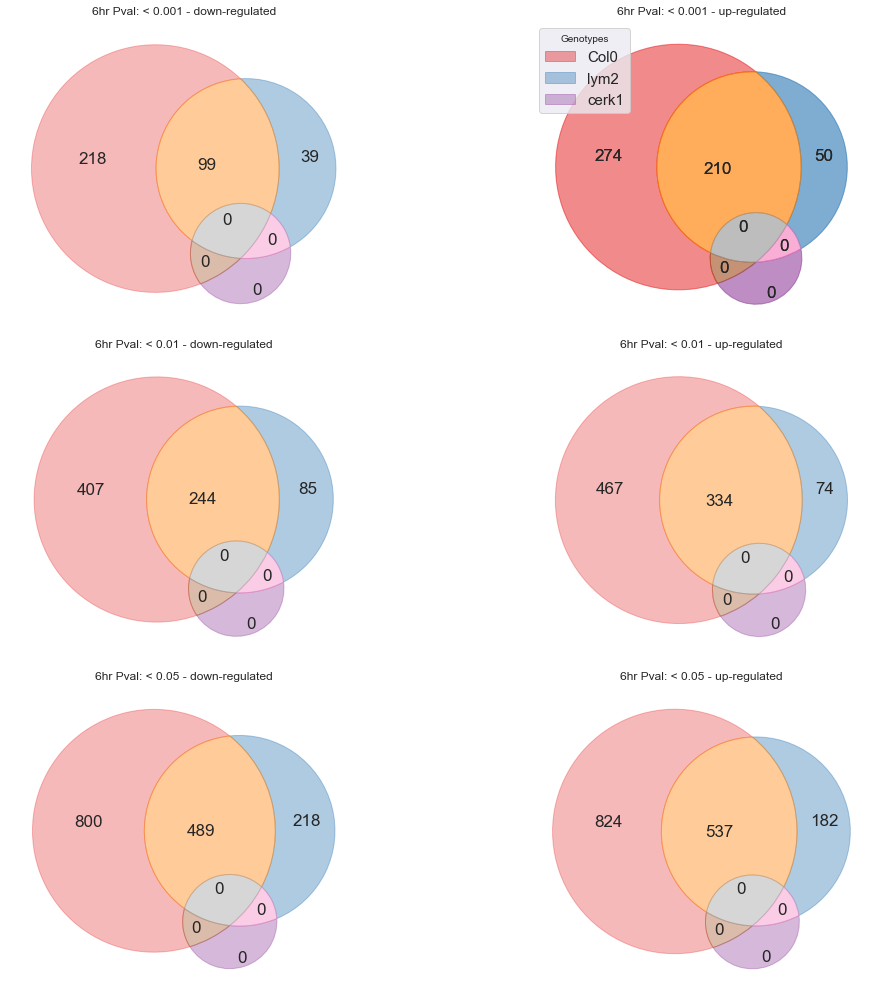
\includegraphics[width=10cm]{obipy-resources/vennTreatmentschitin6.png}
\caption{\label{vennTreatments2}
Venn diagram hypothesis of the chitin effect}
\end{figure}
\end{document}